
\chapter[Voltage-gated Ionic Channels]{Voltage-gated Ionic channels}
\label{chap:voltage-gated-ionic}


\def\spot{{\text{spot}}}
\def\Erev{{\text{E}_{\text{rev}}}}
\def\peak{{\text{peak}}}
\def\step{{\text{step}}}
\def\inj{{\text{inj}}}
\def\spot{{\text{splot}}}
\def\leak{{\text{leak}}}
\def\loss{{\text{loss}}}
\def\out{{\text{out}}}
\def\ion{{\text{ion}}}
\def\axial{{\text{axial}}}
\def\Vcond{{\text{Vcond}}}
\def\Vstep{{\text{Vstep}}}


\section{Introduction}
\label{sec:introduction}

The presence of a transmembrane potential ($\Vm$) -
Sect.\ref{sec:transmembrane-potential} is experimentally confirmed by the
presence of voltage-gated ionic channels which are transmembrane proteins.
In this chapter, we look further by examining voltage-gated ion channels
(Sect.\ref{sec:Voltage-and-Ligand-activated-channels}).

As the gradient of ion concentrations relates to the homeostasis which
eventually affects the normal function of the cell, it's more important to know
the ion concentrations change inside of the cell than the fraction of channels
in each state. However, this is often neglected and often the measurement is
based on dynamics of membrane potential change, in the form of action potential
(Sect.\ref{sec:action-potential}).

The membrane potential ($\Vm$) is a function of the ionic currents through the
opening ion channels and is often modeled as a parallel RC circuit
(Sect.\ref{sec:circ-cell-membr}).

\subsection{Transmembrane proteins as ion channels}
\label{sec:intro-channel-and-membrane}
%\subsection{Ion channels and Biological Membranes}
%\section{Voltage + Ligand-activated ion channels}
\label{sec:ion-channel}

Due to the nature 'blocking' function of biological membranes
(Sect.\ref{sec:membrane-natural-barrier}), to allow charged molecules to diffus
across the membrane, there are transmembrane proteins serving as ion channels on
it.

Ion channels provide a high conducting, hydrophilic pathway across the
hydrophobic interior of the membrane. The pore structure of the ion channel thus
can transport charged molecules across the low dielectric medium
(Sect.\ref{sec:structure}).
The conformational change between closed and open state is called gating, as in
opening and closing a gate (Sect.\ref{sec:channel-gating}).

\subsection{Structure of an ion channel}
\label{sec:structure}

{\bf Ion channels} (or pore structures) are protein complexes that
reside on the biomembrane of cells and their function is to facilitate
the diffusion of ions across biological membranes. Nearly all types of
cells we see today are highly dependent on the actions of these ion
channels to transfer ions in and out of the cell.
Channels are in fact {\it ion selective},
i.e. they can discriminate between size and charge of the ions
(Sect.\ref{sec:permeability-ions}).

\begin{mdframed}
Transmembrane proteins that do not permeate ions; yet can transduce
intra-cellular signal via changing its conformation are called receptors.
Example are G-protein coupled receptors (Sect.\ref{sec:GPCR}).
\end{mdframed}

The role of ion channels, along with {\it mitochondrial membranes}, is
essential for life. Without it, the use of ion gradients which are
necessary for the production of chemical energy (ATP) and therefore
life itself would be impossible.


The two widely known structures are porins and $\K$-channels (both of bacterial
origin).  Much information about the 3D structure of an ion channel was known first with
bacterial $\K$ channel, Fig.\ref{fig:KcsA_channel}. As a matter of fact, the
naming conventions of many ion channels are based on these two known structures. Here, we briefly
introduce porins (Sect.\ref{sec:porin}) - the first structure to be resolved at
atomic resolution <0.3nm \citep{cowan1992}.

Essentially, a  channel is typically a tetramer, i.e. with 4 subunits. They
occupy about 12nm long and 8nm in diameter, which span 3nm or so of
lipid-bilayer membrane. Each subunit has a few transmembrane domains, N-termnal
and C-terminal, e.g.
Fig\ref{fig:Shaker_gene}.

\begin{figure}[hbt]
  \centerline{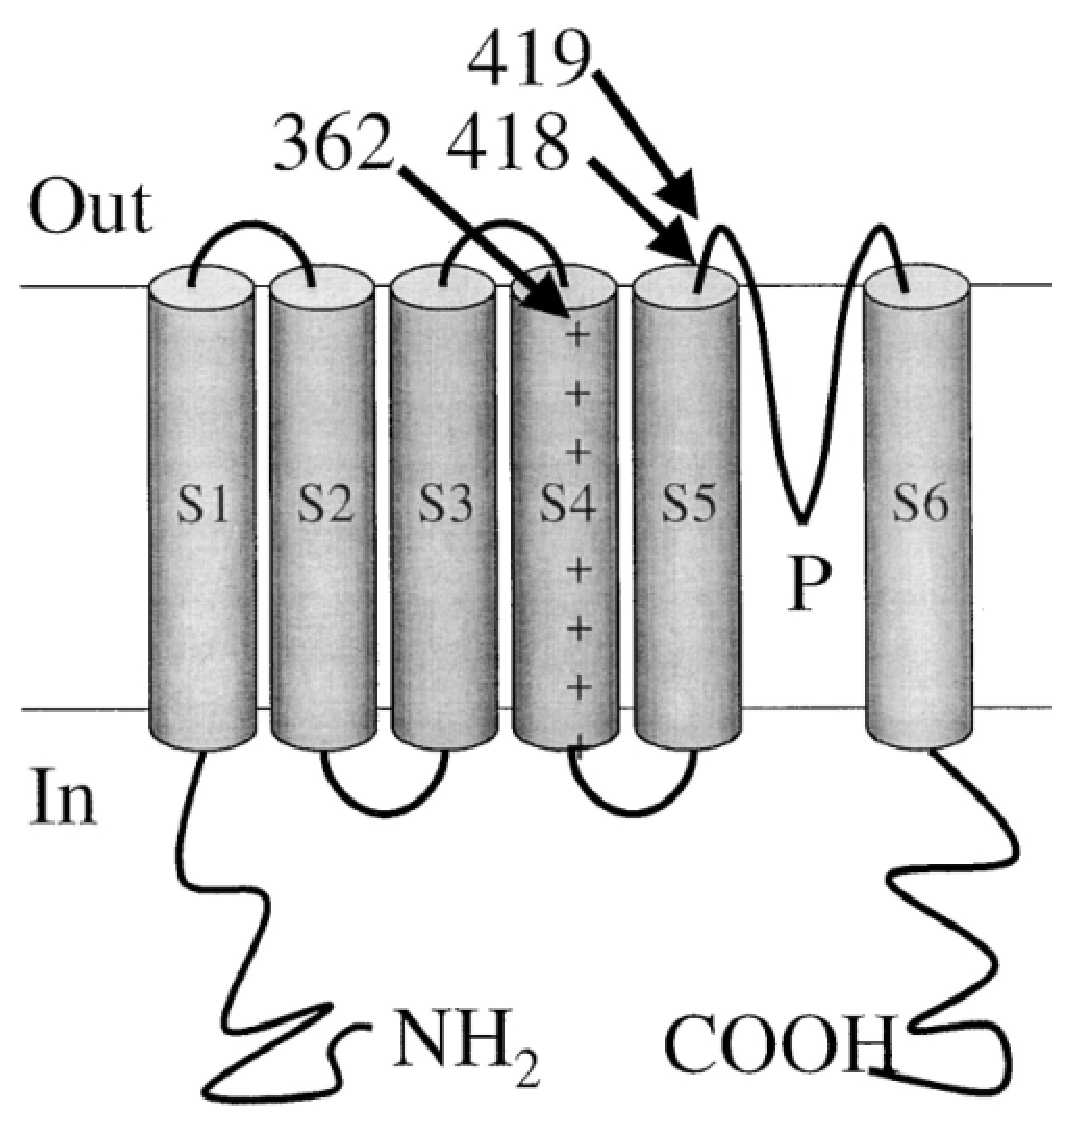
\includegraphics[height=4cm,
    angle=0]{./images/Shaker_gene.eps}}
  \caption{A topology for transmembrane channel's subunit of Shaker gene}
\label{fig:Shaker_gene}
\end{figure}

\begin{enumerate}
  \item a channel is a tetramer with 4 subunits with (1) a narrow
    selectivity filter on the outer side, (2) a vestibule in the
    middle of the membrane. Carbonyl oxygen lines the inner wall of
    the selectivity filter, forming transient binding sites for
    dehydrated $\K$ ions.

  \item each subunit contributes 2 transmembrane helices, forming a
    cone, with its wide end facing the outside of the cell where $\K$
    exit the channel.
  \item two $\K$ ions occupy sites in the selectivity filter, and the
    third one is located in the center of the vestibule.
\end{enumerate}

Some domains can function as a voltage-sensor, or a binding site for
ligand-binding. For the former case, under the influence of a transmembrane
voltage $V_m$, the charged protein residues relocate, changing the tertiary
structure of the ion channel protein, thus allowing selected species of ions to
go through.

The 3D structore of most ion channels are discussed in details in different
chapters (K+ channel - Chap.\ref{chap:potassium-channels}, Na+ channel -
Chap.\ref{chap:Na_models}, Ca2+ channel - Chap.\ref{chap:Ca-channel-models}).

% An ion channels in general has 4 parts:
%
% \begin{enumerate}
%
%   \item a central conduction pathway (formed by the subunits) for ions to pass
%   through
%
%   \item an ion recognition site to allow passage of specific ions
%   (selectivity filter),
%
%   \item domains that function as one or more gates, i.e. enable the ions
%   to pass through when the channel opens; and blocked if it is closed.
%
%   The  gating of these sensors are determined by the sensor domains below.
%
%   \item a sensor that senses the triggering signal and transmits it to
%   the gate to open/close the gate.
% \end{enumerate}

% \begin{figure}[htb]
%   \centerline{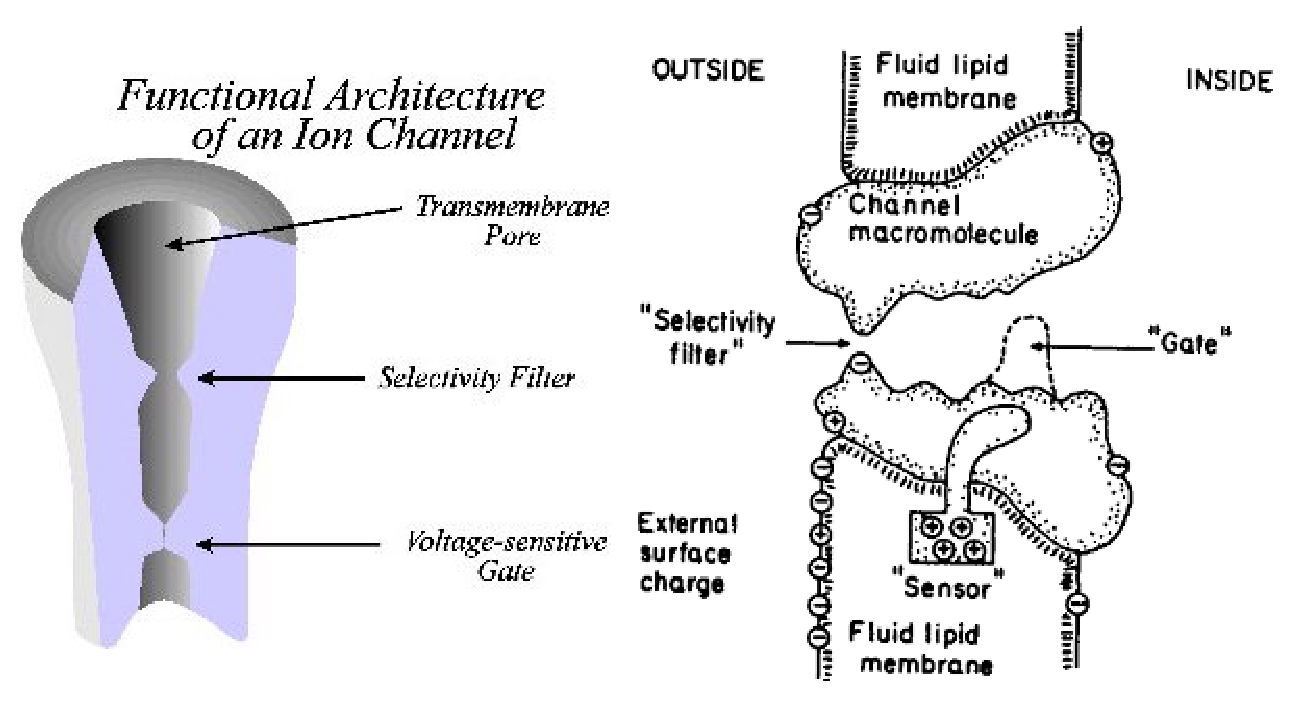
\includegraphics[height=7cm]{./images/ionchannel_structure.eps}}
%   \caption{Ion channel structure}\label{fig:ionchannel1}
% \end{figure}


\subsection{Classification of ion channels: : Voltage + Ligand-activated ion
channels}
\label{sec:class-ion-chann}
\label{sec:voltage-gated-ion-channel}
\label{sec:Voltage-and-Ligand-activated-channels}
\label{sec:Ligand-and-Voltage-activated-channels}

  The main type of stimuli to open an ion channel are (1) Voltage (voltage-gated
  channel), (2) mechanical stress (mechanically-gated channels), (3) binding of
  ligand (ligand-binding channels). The ligand can be extracellular (e.g.
  neurotransmitter (transmitter-gated channels)), or intracellular stimuli
  (ion-gated channels or nucleotide-gated channels). In addition, the activity
  of an ion channels is also regulated by protein phosphorylation or
  dephosphorylation. Mechanically gated channels often have cytoplasmic
  extension that link to the cytoskeleton.


\begin{figure}[htb]
  \centerline{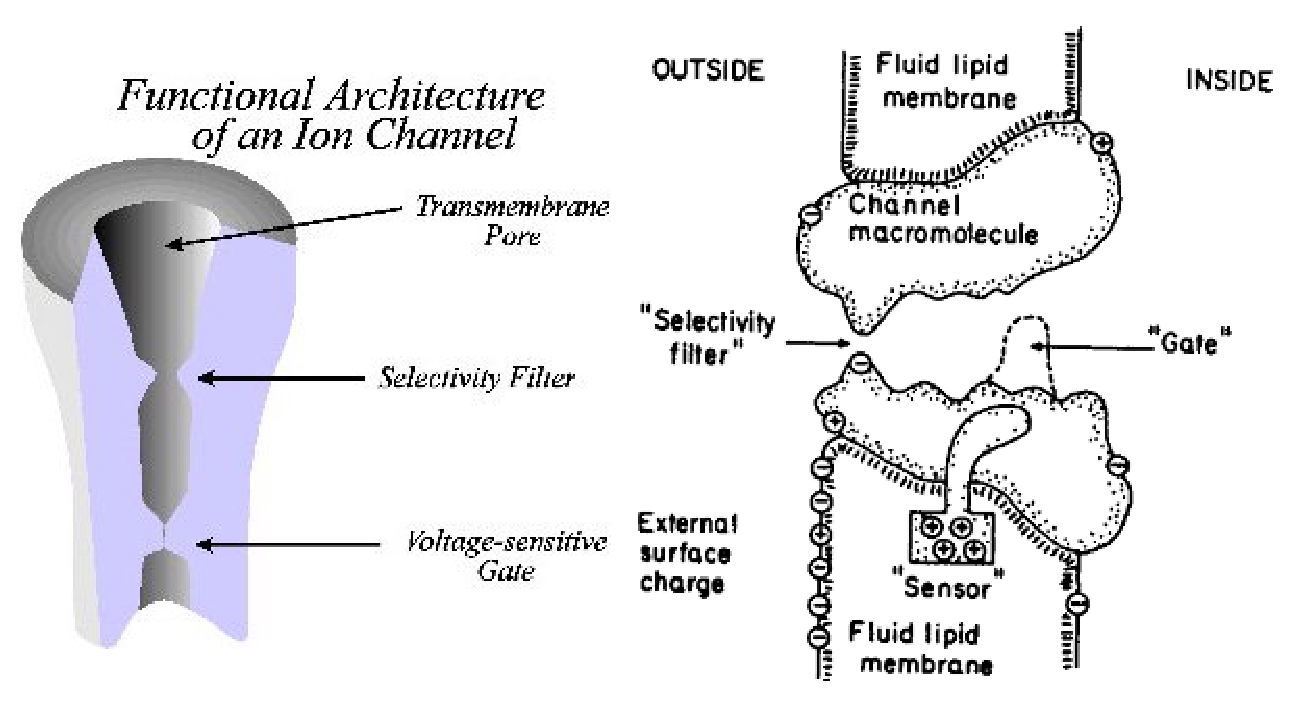
\includegraphics[height=4cm]{./images/ionchannel_structure.eps}}
  \centerline{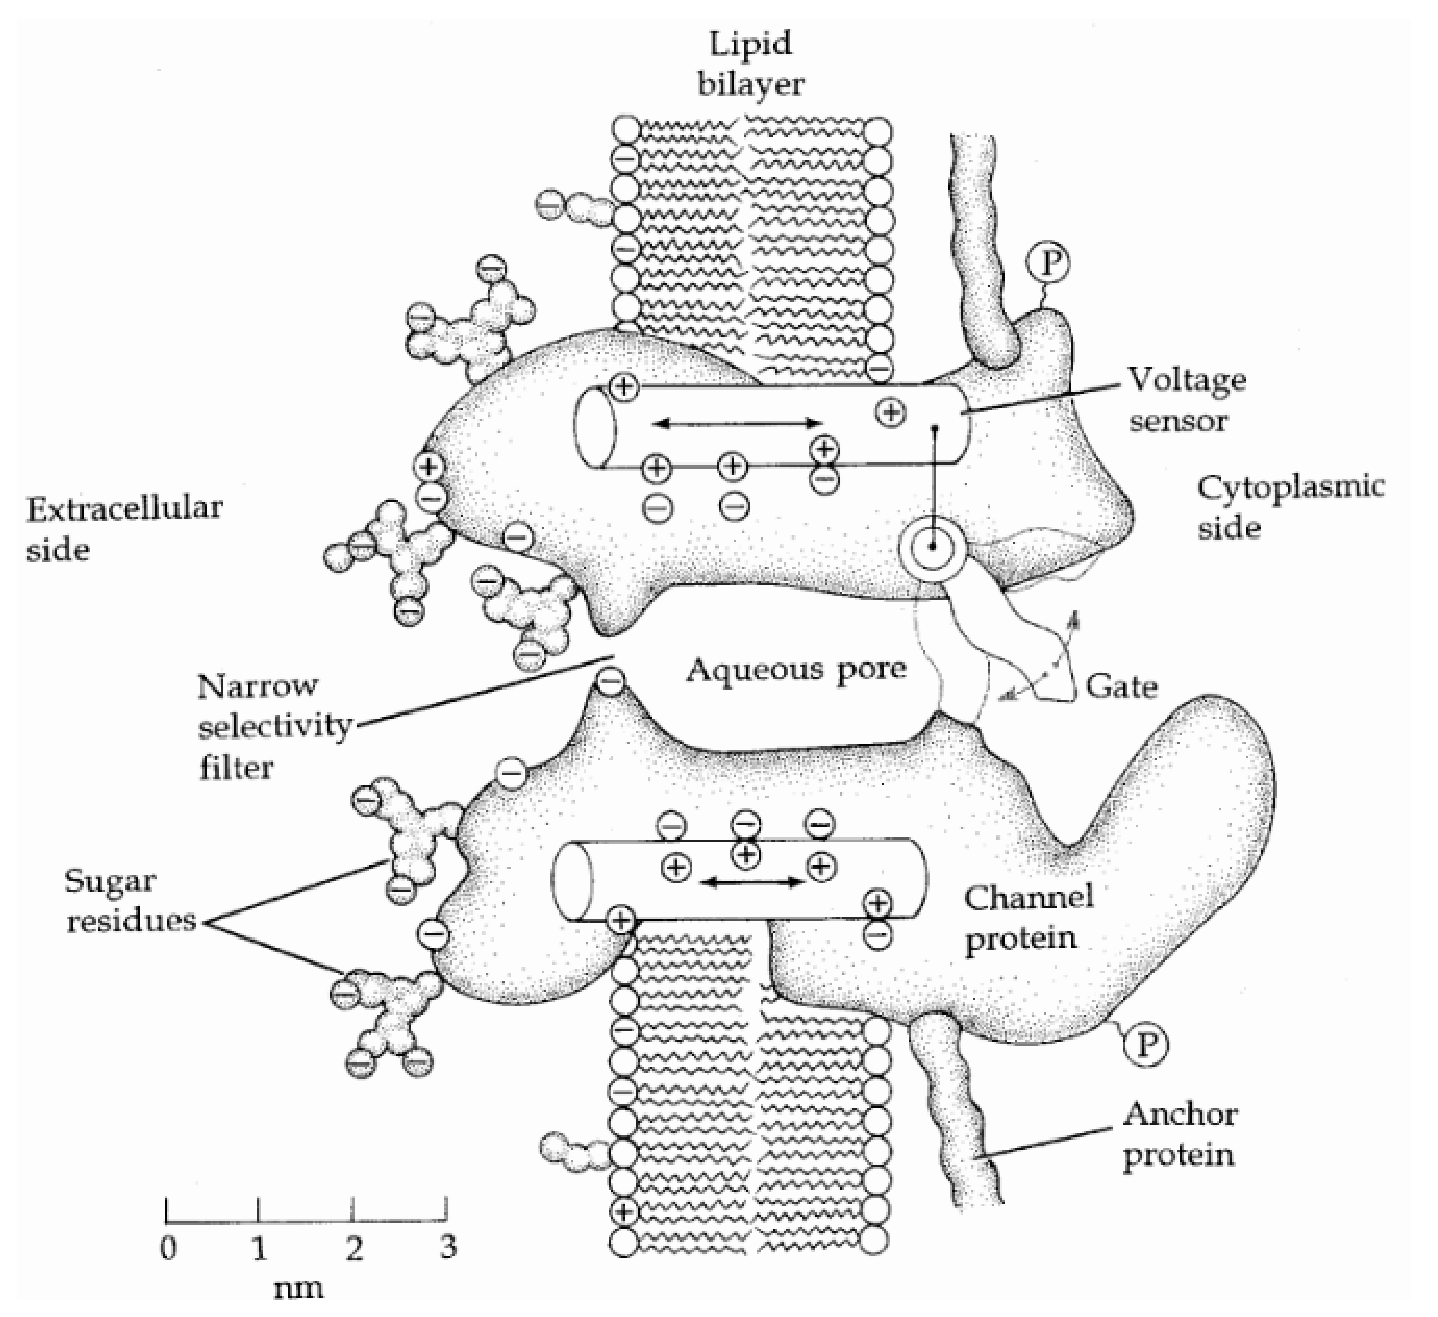
\includegraphics[height=4cm]{./images/cartoon_ion_channel.eps}}
  \caption{A cartoon of an membranous ion channel: A portion of the
    transverse membrane protein form a ``gate'' that is sensitive to
    membrane potential, allowing the pore to be in open or closed
    state}\label{fig:cartoon_ion_channel}
\end{figure}

Typically, we'll focus on voltage-gated ion channels
(Sect.\ref{sec:membrane-potential}), Fig.\ref{fig:cartoon_ion_channel}.
A common way to classify voltage-gated ion channels are based on the ions that
it transports dominantly (Sect.\ref{sec:selectivity-ion-channel}). E.g. an ion
channel permeate to \ce{Ca^2+}, \ce{Sr^2+}, \ce{Ba^2+}, yet the permeability of
\ce{Ca^2+} is the highest. Thus, it is reasonable to name the ion channels to
the type of dominant ions across that channel, e.g. \ce{Ca^2+}-channels,
\ce{Na+}-channels, \ce{K+}-channels, \ce{Cl-}-channels.
% Based on the selectivity of the different ion channels, each type is given a
% different name:
\begin{itemize}
\item \ce{K+} channels (potassium ion channels)
\item \ce{Na+} channels (sodium ion channels)
\item \ce{Ca^2+} channels (calcium ion channels)
\item \ce{Cl-} channels
\item Non-selective cation channels
\end{itemize}
In addition, depending on how fast/slow the channel react to the change in
membrane potential, and/or the direction of the ion transport, the channels can
be classified into detailed classes: e.g. $I_\Ktof$ (transient outward and fast
$\K$ channel) and $I_\Ktos$.

For each type of ion channel, there are different subfamilies. Ion channels are
not restricted to excitable cells only.  There are more than 100 types of ion
channels have been discovered so far with different way to categorize them
(Sect.\ref{sec:class-ion-chann}). A single neuron may contain more than 10 types
of ion channels on the plasma membrane. Probably, the most common ion channels
are \ce{K+} channel, which are found in the plasma membrane of almost every
animal cell.


Ion channels can be classified according to which chemical or physical
modulator controls their gating activity (Sect.\ref{sec:class-ion-chann}).
\begin{itemize}
  \item Transmembrane potential $V_m$-gated channels (electric field): sensitive
  to membrane potential

  \item ligand-gated channels (neurotransmitters, $\Ca$)

  \item second-messenger-gated channels nucleotides (G-protein)

  \item Mechano-sensitive channels osmotic pressure, membrane curvature:
  influenced by membrane strain

  \item Gap junctions (porins not gated, not selective to specific ions)
\end{itemize}

% It can also be classified based on the activators, e.g. voltage-gated or
% ligand-binding gated.

\begin{mdframed}

{\bf Knowledge base}: In practice, the activation/inactivation of ion channels
are regulated by some activators/inhibitors. Such affectors can be membrane
potential ($V_m$), or chemical ligands (agonists/antagonists), or both the two
factors. Thus, ion channels can be classified based on these activators:
\begin{itemize}
  \item ligand-gated ion channels (either activation or
  inactivation). The ligand can be extracellular stimuli
  (e.g. neurotransmitter) or intracellular stimuli (i.e. ion-gated
  channels or nucleotide-gated channels)

  \item voltage-gated (voltage-activated, voltage-operated) ion channels
  which can be depolarization-activated channels or
  hyperpolarization-activated channels.
\end{itemize}
An ionic channels can be both voltage- and ligand-gated channels.

\end{mdframed}
% \end{minipage}

% Typically, as described briefly in previous chapters, ion channels are
% classified according to which chemical or physical modulator controls their
% gating activity .
% \begin{enumerate}
%   \item Ligand-gated ion channels neurotransmitters: sensitive to chemical
%   stimuli, e.g. Second-messenger gated channels nucleotides (e.g. G-protein).
%
% \end{enumerate}



\section{Permeability vs. Conductance}
\label{sec:conductance}
\label{sec:conductance-permeability}

{\bf Knowledge base}: Conductance is closely related to, but not
identical to permeability.

Permeability and conductance are relevant concepts; but they are not exactly the
same.   
\begin{enumerate}
  \item  {\bf Permeability} (Sect.\ref{sec:permeability}) measure the movement
  of mass (which can be either charged or neutral) across the membrane

  \item {\bf Conductance}: movement of positive {\it charge} (e.g.
  opposite direction of electrons) across the membrane.  It is used only for
  movement of charged particles.

Obviously, for charged particles both mass and charge move, so the two things
are not separable. However, it's possible that the particle does NOT move, but
the electrons (which carry charges) move. In that case, i.e. if you had loose
electrons, their movement would be primarily based on conductance, not on
permeability.

Conductance is the reciprocal of resistance  (Sect.\ref{sec:resistance-conductance}).

\end{enumerate}

{\bf Permeability is easier to measure; but measuring conductance is not easy in
cell.}


\section{Permeability of Ion Channels}
\label{sec:permeability-ions}



\begin{mdframed}
  {\bf Knowledge base}: There are 3 main types of canals that ions can
  be transported through the biomembrane:
  {\it ion pumps/transporters}, {\it exchangers} and
  {\it ion channels}.  Both ion pumps and exchangers use ATP energy to
  transport the ions in the direction against that ion's concentration
  gradient; while the activation of ion channels depends upon the
  electrochemical gradient, e.g. membrane potential $V_m$. 
  
  As using energy, the currents through these exchangers/pumps are called {\it
  active currents}; while those go through the ionic channels are called {\it
  passive currents}.
\end{mdframed}

Sect.\ref{sec:conductance-permeability} explains the different between
permeability vs. conductance.

\subsection{Selectivity of ion channels}
\label{sec:selectivity-ion-channel}

Two important properties of ion channels that make it distinguishable
from aqueous pores:

\begin{enumerate}
  \item ion selectivity, i.e. permitting some ions to pass easier, but not
    others.

  \item cannot open continuously, i.e. at single protein level (or single
  channel level), the recorded current showes a random switching between ON and
  OFF state.

\end{enumerate}

{\bf The question is whether a single type of ion or more than one can
  go through a channel?}
- This is an active research in the early time of electrophysiology.

\begin{enumerate}

  \item  Some channels permeate more than one types of ions, e.g. $\Ca$ channels
  permeate not only calcium, but also to $\Na,
  \K$~\citep{meves1973cic,reuter1977sic}. 
  
  
Example: $\K$ channels can conduct $\K$ ions 10,000-fold better than $\Na$,
though both ion species are of the same size (a featureless sphere with
similar diameter: 0.133nm vs. 0.095nm) and the same charge. However, only a
single amino acid substitution can cause the channel to lose this capability.
  
  \item As the ion concentration gradients are different for different ions, the
  driving force or the permeability are different between ion species.

  Example: there's a strong driving force ($V_m-E_\rev$) for $\Na$
  ions (due to the strong positive of $E_{\rev,\na}$, but a weak driving force
  on $\K$ ions (due to $E_{\rev,\k}$ near the resting membrane potential, so
  this driving force only become strong once the AP reach the peak).

  \item On the other hands, the permeability for $\K$ is high, but membrane
  permeability to $\Na$ is low. When the overall permeability
  for different ion species are different and the Goldman equation is applied
  \citep{goldman1943pir}.

\end{enumerate}

\begin{mdframed}

   There is no channel permeable to a single ion only,
  i.e. no channel is perfectly selective. \ce{Na+}-channel in axon is fairly
  permeable to \ce{NH4+} ions and even slightly permeable to \ce{K+} ions.
Even though an ion channel permeate not to a single type of ion, typically
one of them has the dominant permeability.


  A single opening channel can permeate up to 100 million ions per
  second, a rate of $10^5$ times greater than the fastest rate of
  transport mediated by any known protein. However, the ion channel
  cannot couple to any energy source to perform its function. So, the
  transport is always passive, i.e. ``downhill'' from high
  concentration to low concentration. This is known as passive
  transport; while transport via exchanger/pump is called active
  transport as they requires ATP. Models for these active transports will be
  discussed in Chap.~\ref{chap:models-pumps}.
\end{mdframed}


The amazing capability of ion channels to select ions for permeation was
revealed when the crystal structure of the bacterial $\K$ channel was resolved,
Fig.~\ref{fig:KcsA_channel}. Typically, a cation is surrounded by water
molecules due to electrostatic force, and the ion channel's pore size is too
small for them to go through. So, at first, the water molecules surrounding
the ion need to be removed for the ion to go through.


\begin{figure}[hbt]
  \centerline{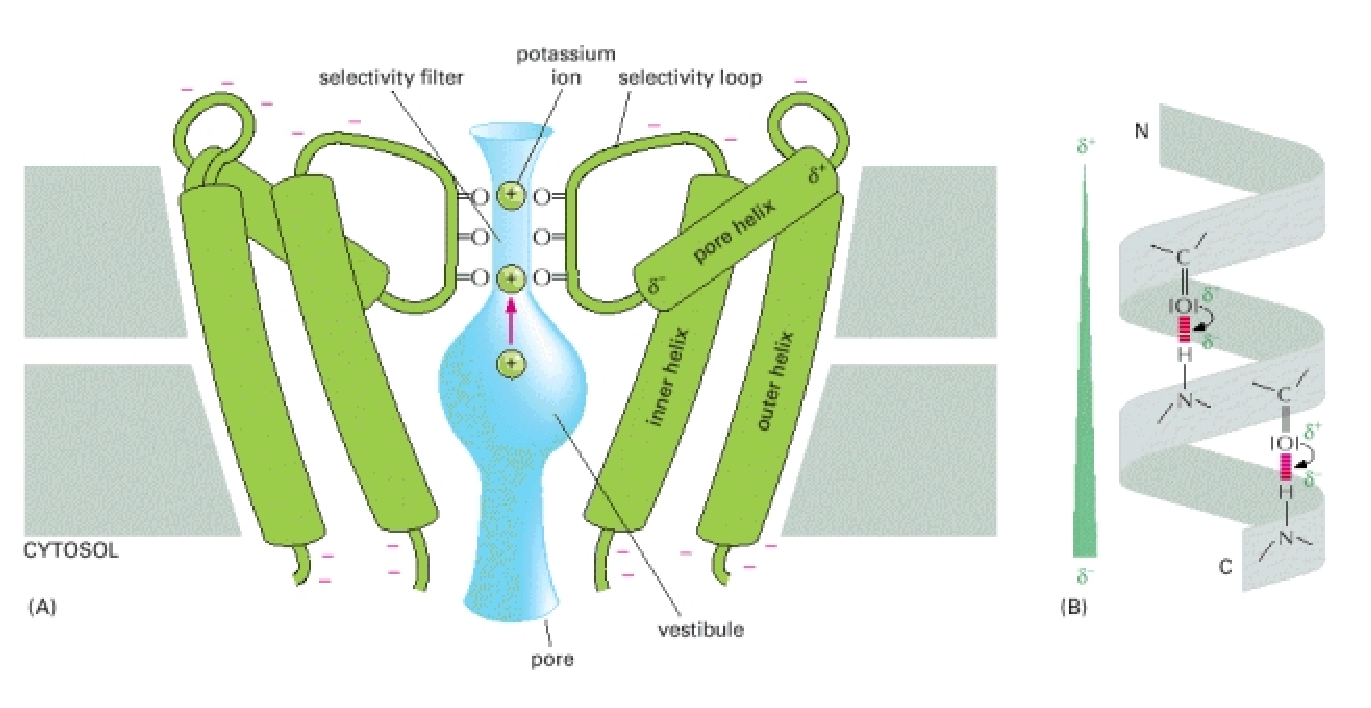
\includegraphics[height=5cm, angle=0]{./images/K_channel.eps}}
  \caption{The structure of bacterial $\K$ channel's subunit}
  \label{fig:KcsA_channel}
\end{figure}

\subsection{permeability}
\label{sec:permeability}


Consider the next flux $\bar{m}$ of an ion
\begin{itemize}
  \item $\bar{m}$ is positive for inward current of positive ions

  \item the inward flux is $m_i$ (positive), and the outward flux is $m_o$
  (negative)

  So, $\bar{m} = m_i + m_o$

  \item the net flux as a function of ion permeability $P$, and concentrations
  $c_o, c_i$

\begin{equation}
\label{eq:net-flux}
\bar{m} = P \times (C_o - C_i \exp\left( E_\rev.F/(RT) \right)) \times f(E_\rev)
\end{equation}
with $E_{\rev}$ is (inside-outside) reversal potential.

The factor $f(E_{\rev})$ describes potential dependence of the flux.
This is NOT a constant-field derivation.

\end{itemize}
At reversal potential for a single type of ion channel (or resting potential in
case of different types of ion channels), the total chages movement is zero
\begin{equation}
\label{eq:net-flux-balance}
z_1 \bar{m}_1 + z_2 \bar{m_2} + \ldots + z_n \bar{m_n} = 0
\end{equation}
with $\bar{m_i}$ is the next flux of ion $i$ of valance $z_i$.


The {\bf permeability} of an ion is defined as $P$ [cm/sec]
\begin{equation}
  \label{eq:1243}
  P = \frac{D.\beta}{h}
\end{equation}
NOTE: P (cm/sec) is equivalent to 10*P ($\mum$/ms).

\begin{mdframed}

The units of permeability $P$ are indeed: cm$^3$ / (sec . cm$^2$), as P = D/L,
with D=diffusion constant, L=membrane thickness. 

\begin{verbatim}
permeability * concentration_difference * surface_area = flux
\end{verbatim}

\end{mdframed}

IMPORTANT: $P$ is not a constant but can be a function of something
else, e.g. transmembrane voltage or ion gradient
(Sect.\ref{sec:permeability-non-electrolyte-ion}). In many cases, this
permeability is defined as a function of trans-membrane voltage $\Vm$ -
Sect.\ref{sec:permeability-Voltage-dependence}.

then the electric current density is
\begin{equation}
  \label{eq:1244}
  J =  -\frac{P.V_mz^2F^2}{RT} \frac{\beta_ic_i-\beta_o c_o\exp(-V_m\frac{zF}{RT})}{1-\exp(-V_m\frac{zF}{RT})}
\end{equation}
Using this equation, if we consider a channel is permeated to more
than one ion, say calcium-channel is not perfectly selective to calcium, but is
permeated by $\Ca, \Na$ and $\K$ ions with 3 different permeability $P_\ca,
P_\na, P_\k$ then at equilibrium (or at reversal potential $E_m$ of that
calcium channel), the net flux is zero 
\begin{equation}
  \label{eq:1246}
  J = J_\ca + J_\na + J_\k = 0
\end{equation}
or
\begin{equation}
  \label{eq:1247}
  \begin{split}
    P_\k\left[c_{i,\k} - c_{o,\k}\exp (-\frac{E_mF}{RT}\right] &+
    P_\na\left[c_{i,\na} -
      c_{o,\na}\exp (-\frac{E_mF}{RT}\right] + \\
    &P_\ca\left[c_{i,\ca} - c_{o,\ca}\exp (-\frac{E_mF}{RT})\right] = 0
  \end{split}
\end{equation}
or
\begin{equation}
  \label{eq:1248}
  P_\k c_{i,\k} +   P_\na c_{i,\na} +   P_\ca c_{i,\ca}  =
  \exp(-\frac{E_mF}{RT}) \left(  P_\k c_{o,\k} +   P_\na c_{o,\na} +   P_\ca c_{o,\ca} \right)
\end{equation}
and the membrane potential at which the (net) membrane current is zero
is called the {\bf reversal potential} $E_m$ which is defined via the
so-called {\bf Goldman-Hodgkin-Katz} (GHK) equation as follows
\begin{equation}
  \label{eq:1249}
  E_m = -\frac{RT}{F} \ln \frac{P_\k c_{i,\k} +   P_\na c_{i,\na} +   P_\ca c_{i,\ca}}{P_\k c_{o,\k} +   P_\na c_{o,\na} +   P_\ca c_{o,\ca}}
\end{equation}


Normally, permeabilities are reported relatively to $P_{\ce{K+}}$ as in
most nerve cells at rest, $P_{\ce{K+}}$ is larger than $P_{\ce{Na+}}$ and
$P_{\ce{Cl-}}$. The permeability ratio of $\K$ ions to $\Na$ ions
\begin{equation}
P_K : P_\Na = \frac{-\left( \exp( E_\rest .F .z_\k / (RT)) \right) [\K]_i +
[\K]_o}{ \exp( E_\rest .F .z_\na / (RT)) [\Na]_i + [\Na]_o}
\end{equation}
\begin{enumerate}
  \item In MSN (Sect.\ref{sec:medium_spiny_neurons})

Nisenbaum et al. (1996)
\begin{verbatim}
P_K : P_Na = 49 : 1
\end{verbatim}

  \item General use:
  \footnote{\url{http://www.csupomona.edu/~seskandari/physiology/physiological_calculators/ghk_equation.html}}.

  \begin{eqnarray}
    \label{eq:539}
    P_{\ce{K+}}:P_{\ce{Na+}}:P_{\ce{Cl-}} = 1:0.05:0.45
  \end{eqnarray}

  \item The permeability can also represented as a function of voltage -
  Sect.\ref{sec:permeability-Voltage-dependence}
  \label{sec:GHK-Ca2+}
\begin{equation}
P_\Ca = P(\Vm)
\end{equation}
\end{enumerate}

\subsection{-- non-electrolyte ion}
\label{sec:permeability-non-electrolyte-ion}

In solubility-diffusion theory, the permeant of non-electrolyte ions is
determined by the intramembrane ion concentration gradient. If the membrane
thickness is $h$, with concentration gradient $\Delta c$, given that $S$ denotes
the ion, then the molar flux density $M_S$
\begin{equation}
M_S = -P_S \Delta c_S
\end{equation}
$P_S$ (cm/s) is membrane permeability, $M_S$ (mol/cm$^2$.s) molar flux density
of S.

If the partition of S between water and membrane occurs rapidly and considered
as equilibrium, we only consider the effect of concentration gradient within the
membrane $\Delta c_S.\beta_S$, with $\beta_S$ (dimensionless) water-membrane
partition coefficient for S. Using Fick's first law, the new equation is
\begin{equation}
M_S = - \frac{\Delta c_S D_S \beta_S}{h}
\end{equation}

$D_S$ is diffusion constant of S within the membrane. Then, the permeability can be determined using
\begin{equation}
P_S = \frac{D_S.\beta_S}{h}
\end{equation}
with $h$ is the thickness of the membrane.


\begin{figure}[hbt]
  \centerline{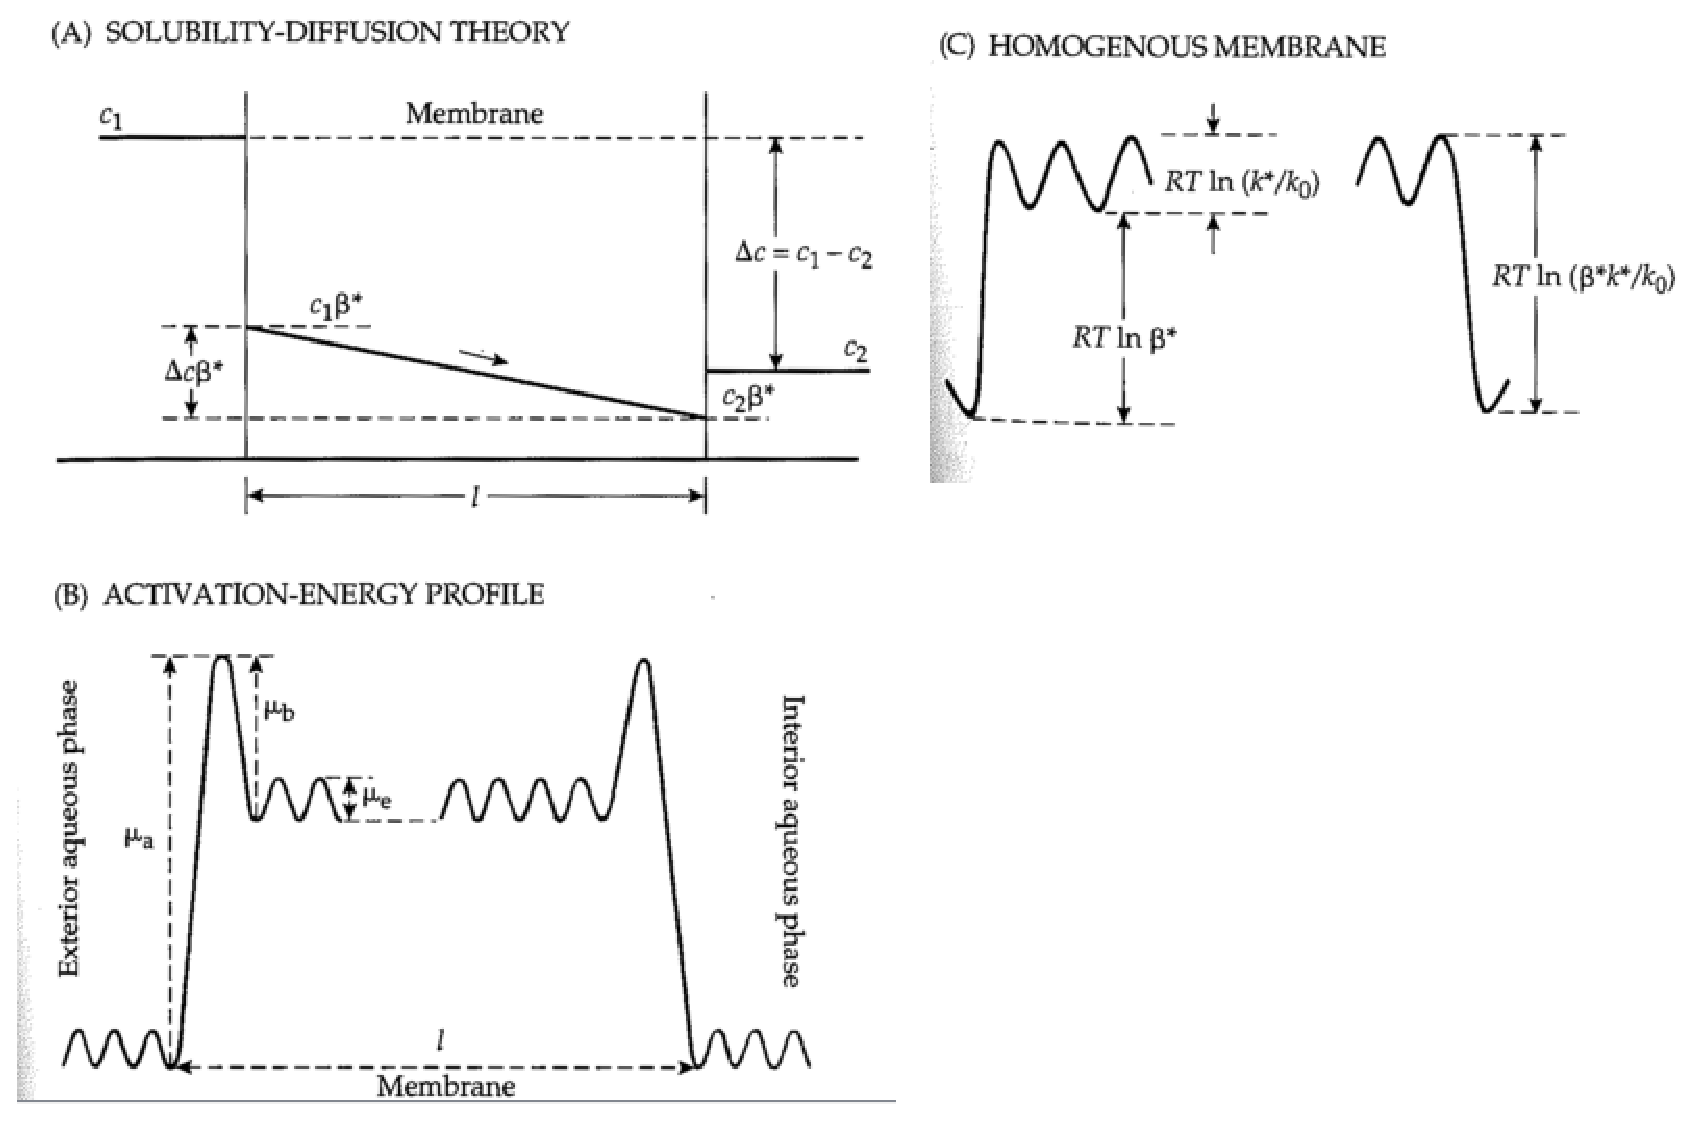
\includegraphics[height=6cm,
    angle=0]{./images/theory_permeability.eps}}
  \caption{(A) Solubility-diffusion theory; (B) Activation-energy profile; (C)
  Homogeneous membrane}
\label{fig:theory_permeability}
\end{figure}

\subsection{-- electrolyte ion}
\label{sec:permeability-electrolyte-ion}

If ion S is an electrolyte, it might see the membrane as a series of
potential energy barriers, which Danielli called $\mu_a$. These energy barriers
are small enough not to be rate-limiting, Fig.\ref{fig:theory_permeability}.

The effective diffusion constant is $D=k\lambda^2$ (Eyring theory -
Sect.\ref{sec:eyring-rate-theory}) or $D=k h^2/n^2$, with $k$ is unidirectional
rate constant for jumping over an energy barrier in the membrane, $\lambda$ is
the distance between energy minima, and $n$ is the number of jumps needed to
cross the membrane. \citep{woodbury1971} derived the formula for permeability
coefficient
\begin{equation}
P_S = \frac{\beta_S k_S h}{n^2}
\end{equation}
However, using these models are quite complicated.

Another theory, by far the most popular, is {\bf constant-field theory}
developed by Goldman (1943) and Hodgkin-Katz (1949) -
Sect.\ref{sec:constant-field-theory}. This is based on continuum-independence
approach, i.e. ion permeations are independent and the energy gradient is
continuum across the membrane.
The two important assumptions are (1) ions transports are independent, (2)
electric field in the membrane is constant (i.e. the potential drop linearly
across the membrane).  It gives rises two equations: GHK current equation
(Sect.\ref{sec:GHK_current}) and GHK voltage equation
(Sect.\ref{sec:GHK_voltage}). Here, the permeability constant is
\begin{equation}
P_S = \frac{D_S\beta_S}{h}
\end{equation}
which is the same as that in solibility-diffusion theory.
% and is defined as the
% D/h (D=diffusion of Na ion across the membrane area, h=thickness of
% the membrane)

\subsection{voltage-dependent permeability}
\label{sec:permeability-Voltage-dependence}

\def\Ba{{\text{Ba}^{2+}}}
\def\Vhalf{{\text{V}_{\text{h}}}}
\def\Vslope{{\text{V}_{\text{s}}}}

In the case of $\Ca$ channel, the permeability of the channel to $\Ca$ or $\Ba$
is a function of trans-membrane voltage $\Vm$, as shown in
Fig.\ref{fig:Ca2+-current-voltage-clamp-Bargas-1994-MSN}.
\begin{equation}
P(\Vm) = \frac{\alpha}{1 + \exp\left( \frac{\Vm - \Vhalf}{\Vslope}  \right)}
\end{equation}

\begin{figure}[hbt]
  \centerline{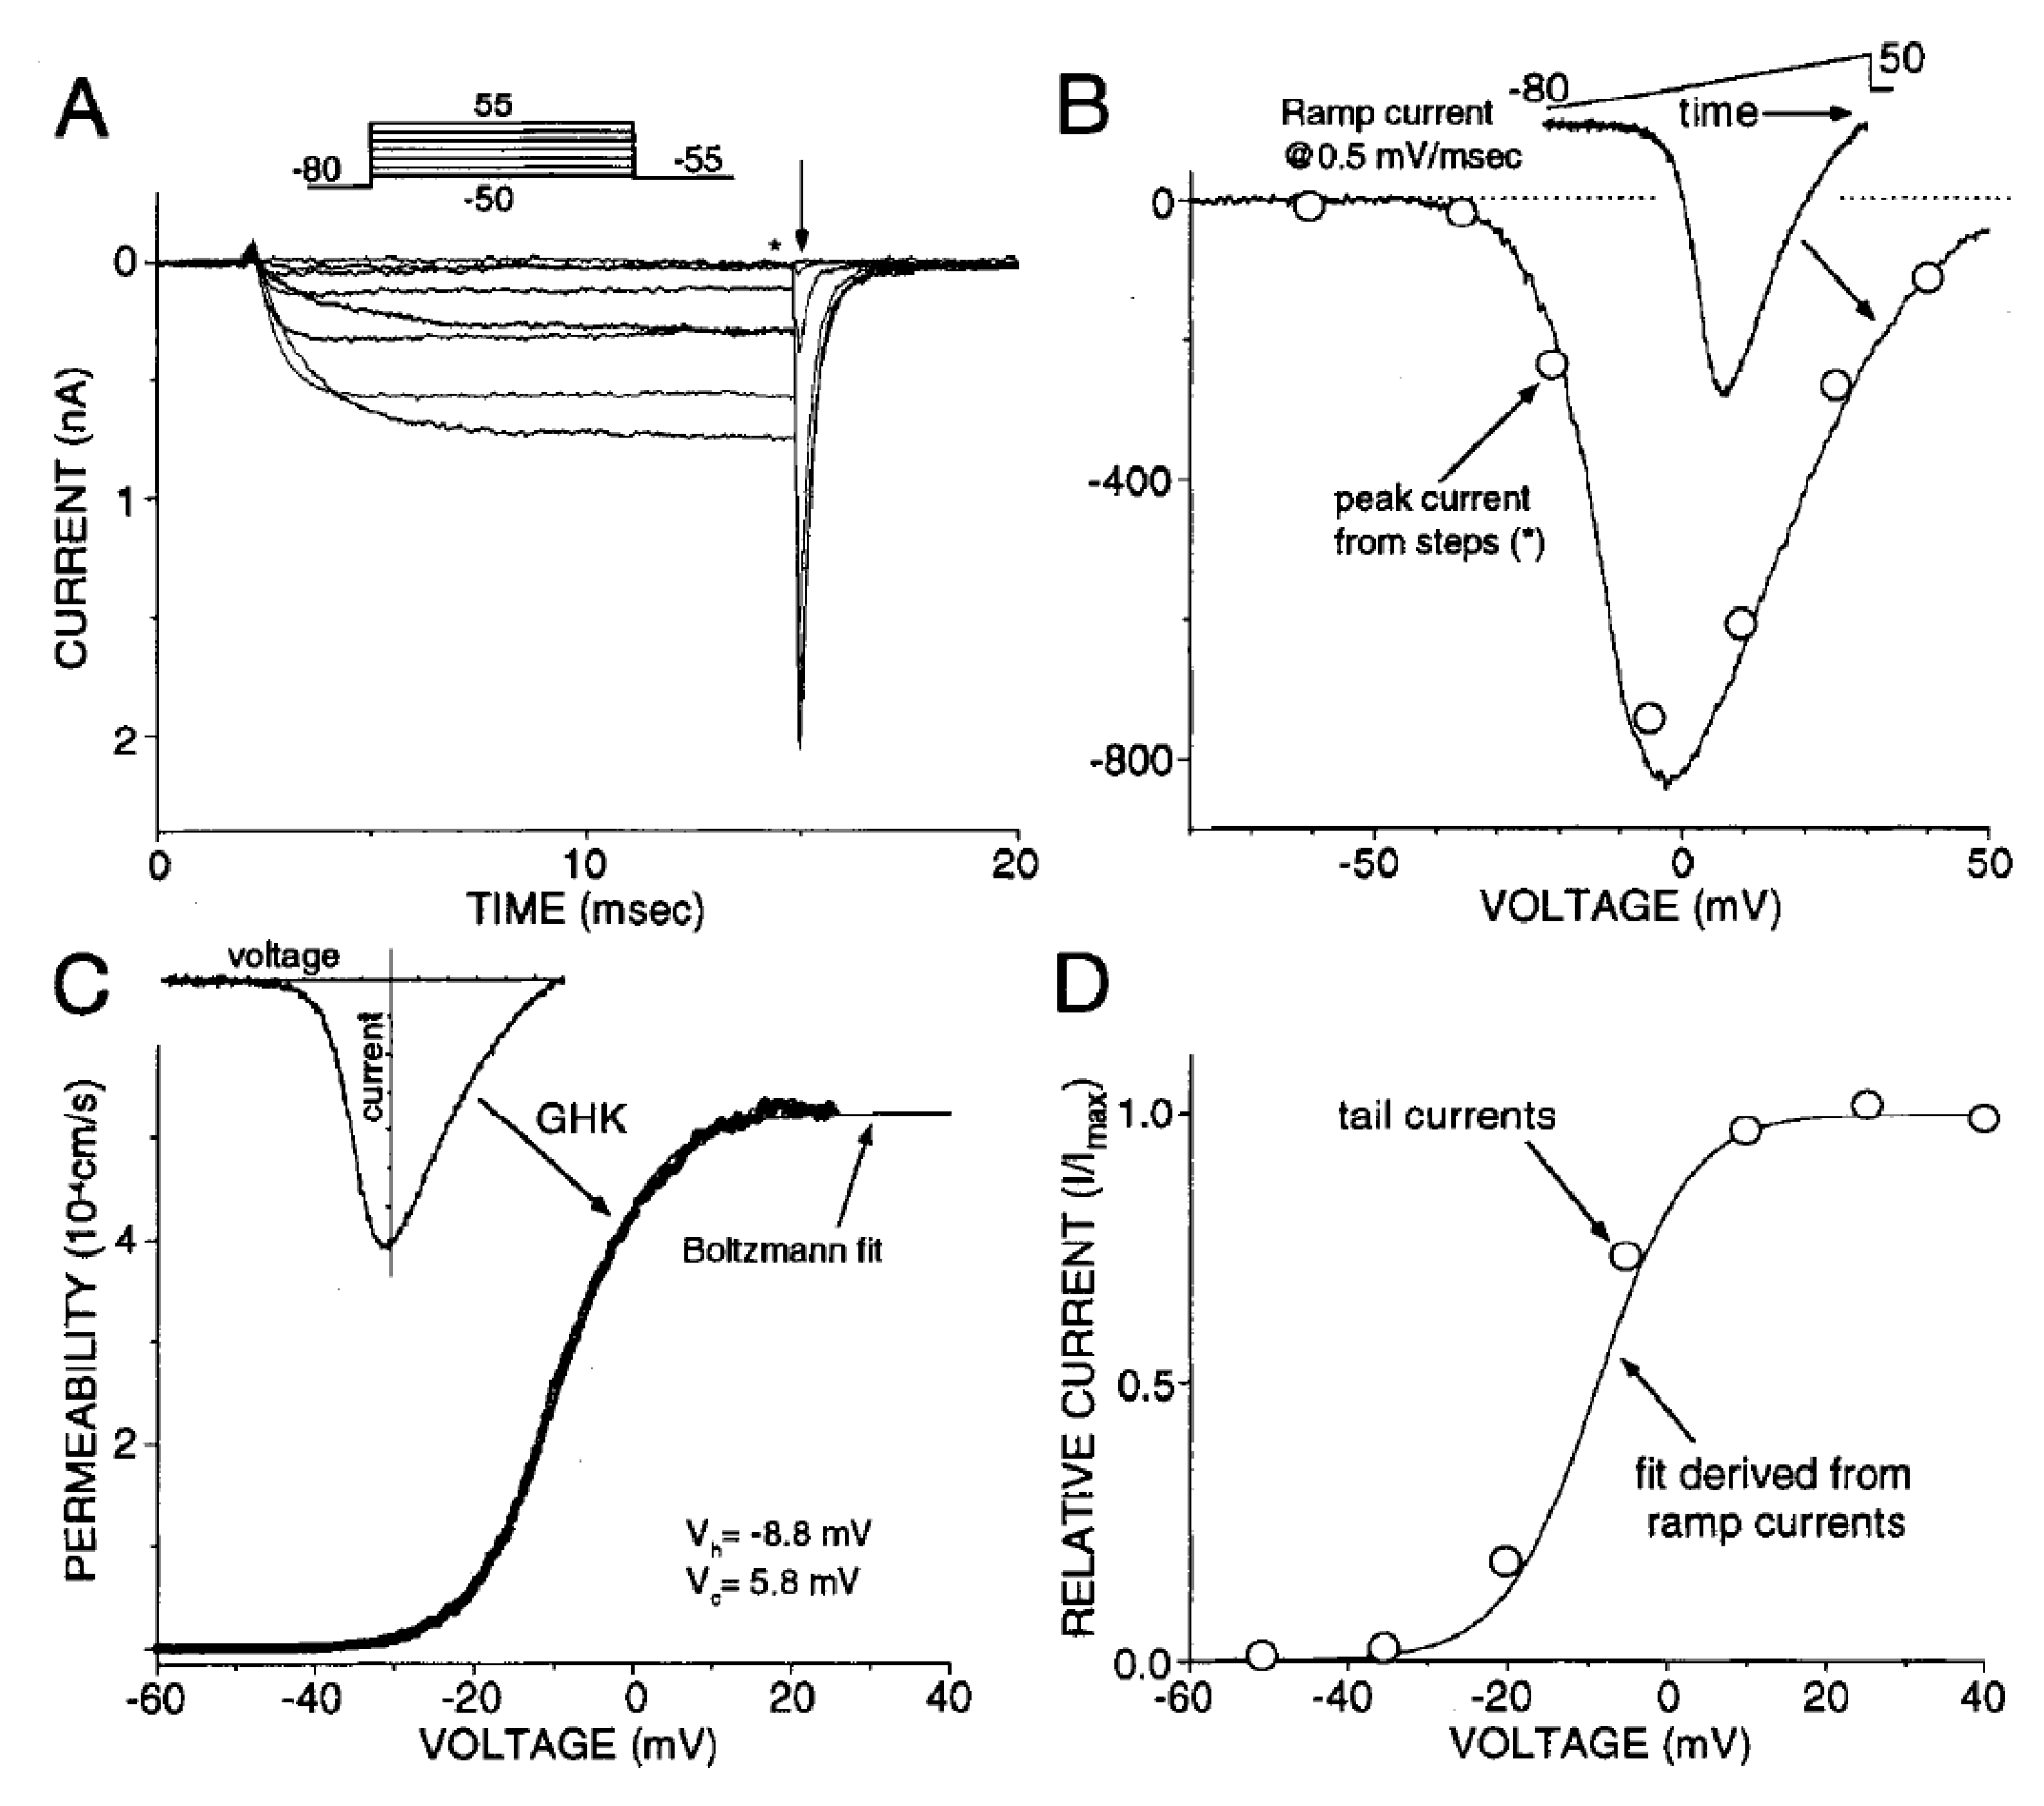
\includegraphics[height=6cm,
    angle=0]{./images/Ca2+-current-voltage-clamp-Bargas-1994-MSN.eps}}
  \caption{Currents activated by step voltage commands and ramps (Bargas et
  al., 1994).
  {\bf (A)} inward currents (including $\Ca$ and leak curent) using holding potential at -80mV;
  then step to different values from -50mV to +55mV with 15mV step; before
  repolarizing back to -55mV (i.e. ramp current). NOTE: The second phase back to
  -55mV is used to estimate the tail current. {\bf (B)} The I-V curve of peak $\Ca$ currents at
  different step voltage in (A) (after
  subtracting leak current). {\bf (C)} The I-V curve in (B) is used to derive
  the permeability trace }
\label{fig:Ca2+-current-voltage-clamp-Bargas-1994-MSN}
\end{figure}


\subsection{single channel permeability}
\label{sec:single-channel-permeability}

If there are $n$ channels in a 1 cm$^2$ patch of membrane, and membrane
permeability is P (cm/sec) - Sect.\ref{sec:permeability}), then the permeability
of a single channel is P/n and also has units of cm/sec.


The permeability of a single ion channel can be defined via the single-channel
unitary current $i_\na$ ($\muA/\muF$ or $\muA/$cm$^2$ depending wherether we
incorporate $\Csc$ in the equation or not), by switching elements in
eq.~\eqref{eq:876}
\begin{equation}
  \label{eq:1351}
P_\na =   \frac{i_\na}{
z_\na^2.V_m\frac{F^2}{RT}\times\frac{\ce{[Na_o]}-\ce{[Na_i]}\exp(z_\na.\frac{V_m-E_{\ce{Na}}}{RT/F})}{1-\exp(z_\na.\frac{V_m}{RT/F})}}
\end{equation}
NOTE: The total membrane ionic current is typically in unit of $\muA$.

To find the permeability for a single channel, say L-type $\Ca$ channel with
unitary current $i_\dhpr$, the formula is (Sect.~\ref{sec:unit-i_cal-curr})
we do similar to eq.~\eqref{eq:1351}
\begin{equation}
  \label{eq:1353}
  P_\dhpr = \frac{i_\dhpr}{z_\ca ^2 \frac{F}{RT/F}V_m
    \left[\frac{\exp\left(\frac{z_\ca V_m}{RT/F}\right)[\ca]_\myo-0.341[\ca]_o}{\exp\left(\frac{z_\ca V_m}{RT/F}\right)
        - 1} \right]}
\end{equation}
Suppose in a cardiac cell, we have $N$ calcium-release units (CaRUs), each one
with $N_L$ $\Ca$ channels, then the whole-cell permeability is
\begin{equation}
  \label{eq:1352}
  P_\dhpr^T = P_\dhpr \times  N \times  N_L
\end{equation}






\section{Equations of Ionic Currents}
\label{sec:equat-ionic-curr}

In this section, we will discuss how we formulate the current via opening ion
channels which form as energy barriers.

The Nernst-Planck equation (Sect.\ref{sec:Nernst-Planck-equation}) describes the
movement of charged ions from one region to another in aqueous media. However,
when the charged ions moving from the extracellular region to intracellular
region across the cell membrane, the cell membrane has thickness and there may
be energy barriers or blocking sites within the channel.
In this case, the \textcolor{red}{ions flowing through the open channel may not
obey the Nernst-Planck equation and we must model the complex behavior within this
membrane}.

There are different treatments
\begin{enumerate}
  \item the simplest one: Hodgkin-Huxley formula using Ohm's law, in which it is
  assumed a linear dependency between the current and the voltage
  (Sect.\ref{sec:ohms-law})

  \item the more complicated one: known as the Goldman-Hodgkin-Katz formula
  using constant-field theory (where the energy barrier drop linearly across the
  membrane), in which the current is a non-linear function of voltage
  (Sect.\ref{sec:GHK_voltage})

  \item the most complicated one: Eyring rate theory (Sect.\ref{sec:eyring-rate-theory})
  with multiple energy barriers
\end{enumerate}


This requires a proper understanding of ion permeabilities
(Sect.\ref{sec:permeability-ions}).
\begin{itemize}
  \item assuming each ion channel transports only one type of ion species.
  Here, the transport is linear. Hodgkin-Huxley model used the linear formula
    (Sect.\ref{sec:ohms-law}).

%  The I-V relation can be linear or non-linear.
%   \begin{enumerate}
%     \item :
%     \item
%   \end{enumerate}

  \item assuming multiple ion species can be transported via the ion channel,
  each with a different membrane permeability $P_S$ (for ion $S$).
  Here,  the transport is non-linear:
  \begin{enumerate}
    \item the transports of different ion species via the single channel is
    independent. The nonlinear relation is represented via
    Goldman-Hodgkin-Katz equation
(Sect.\ref{sec:GHK_voltage}).


    \item the transports of different ion species via the single channel is
    dependent: rate-theory description ionic permeation
    (Sect.\ref{sec:eyring-rate-theory}). The detail discussion for ionic
    currents via ion channels is given in Appendix.~\ref{sec:movement-ion-across-ion-channels}.

  \end{enumerate}

\end{itemize}


\subsection{Ohm's Law}
\label{sec:ohms-law}

During studying the electrical behavior of a cell membrane, it's observed that
the ionic current $I_S$ of some ion species $S$ through the associated ionic
channel can be approximated using linear {\bf Ohm's
law}\footnote{\url{http://en.wikipedia.org/wiki/Ohm's_law}}
\begin{equation}
  \label{eq:50}
  I = \frac{V}{R}
\end{equation}

For ion S, the current can be written in the form
\begin{eqnarray}
  \label{eq:545}
  I_S = g_S (V_m-E_S)
\end{eqnarray}
$E_\rev$ is the potential at which there is no current, so we call it reversal
potential (Sect.\ref{sec:reversal-potential}); $V_m$ [mV] is the transmembrane
potential at the time of analysis and $g$ is the conductance in (mS/cm$^2$) and
$I_\text{ion}$ in ($\mu$A/cm$^2$). Sect.\ref{sec:resistance-conductance}
explains the uses of conductanace $g$ in Ohm's law in cell electrophysiology.
 
\begin{mdframed}
For a cell with multiple ion channels, if all channels are modeled using
Ohm's law, then the total ionic current is

\begin{equation}
  \label{eq:30}
  I_{ion} = I_K + I_{Na} +... = \sum_i g_i (V_m-E_i)
\end{equation}

\end{mdframed}

\begin{figure}[htb]
  % \centerline{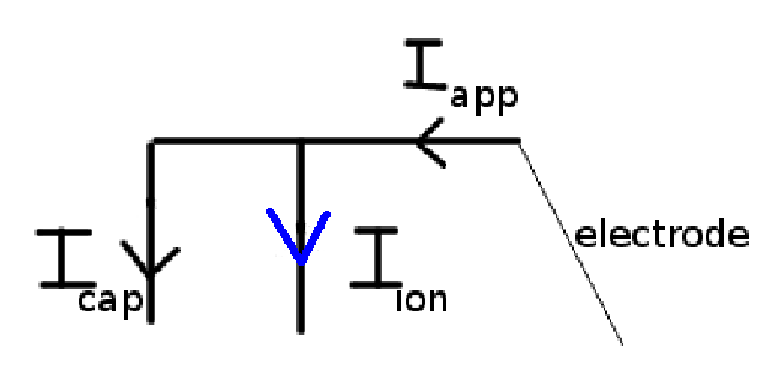
\includegraphics[height=4cm]{./images/electric_current.eps}}
  \centerline{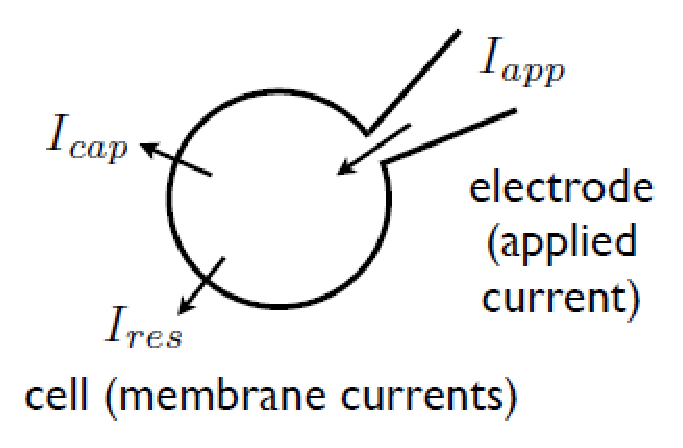
\includegraphics[height=4cm]{./images/current_in_cell.eps}}
  \caption{Electric currents via cell membrane}\label{fig:electric_current}
\end{figure}
 
This linear assumption of the ionic current has been widely used to model the
dynamics of transmembrane potential of excitable cells, e.g.
Sect.\ref{sec:model_HH-based}.


% The formula to find $E_\rev$
% for a channel selective to a single-ion is {\bf Nernst equation}
% (Sect.~\ref{sec:nernst-equation}), and the formula when the channel is
% selective to multiple ions is formulated via the Goldman-Hodgkin-Katz voltage formula
% (Sect.~\ref{sec:GHK_current}).




% If I-V follows a linear relationship, then we can use the simple Ohm's
% law. Thus, the ionic current has the form
% \begin{equation}
%   \label{eq:29}
%   I_{ion} = g (V_m-E_b)
% \end{equation}




\subsection{Goldman-Hodgkin-Katz Current Equation (GHK):
Constant-Field Theory}
\label{sec:constant-field-theory}
\label{sec:GHK_current}
\label{sec:GHK_flux}

\begin{mdframed}
The GHK flux equation is mostly used by electrophysiologists when the ratio
between [S]$_i$ and [S]$_o$ is large and/or when one or both of the
concentrations change considerably during an action potential.
In such cases, the current-potential curve I-V follows a non-linear
relationship. Therefore, we cannot use Ohm's law.
\end{mdframed}

An exact formula for the diffusion of ions in an aqueous media is represented by
Nernst-Planck equation (Sect.\ref{sec:Nernst-Planck-equation}). With the
presence of the plasma membrane of thickness $h$, the electric field can
cause a non-linear relationship between the I-V

Goldman developed the {\bf ``constant field'' theory} to derive the equation of
the movement of ions under the constant field assumption
~\citep{goldman1943pir} (Sect.\ref{sec:permeability-ions}).
\begin{verbatim}
Vo |     |
   |     |
   |     | Vi
   <--h-->
   (membrane)
 ------------------->x
 dV/dx=constant = Vm/h
\end{verbatim}

% When I-V curve  follows a non-linear relationship and the transport of the ions
% across the channels can be assumed independent,

GHK flux equation is a solution to the Nernst-Planck equation
(Sect.\ref{sec:Nernst-Planck-equation}) with the assumptions listed below
\begin{enumerate}
  \item membrane is homogeneous substance
  \item electrical field is constant so that the transmembrane potential varies
  linearly across the membrane
  \item  ions access the membrane instantaneously from the intra- and
  extracellular solutions
  \item permeant ions do not interact
  \item movement of ions is affected by both concentration and voltage
  differences
\end{enumerate}

% using {\bf Goldman equation} (which was later extended to calculate ionic
% current for ion channels (Sect.\ref{sec:GHK_current})

Using Nernst-Planck equation (Sect.\ref{sec:Nernst-Planck-equation}), with the
assumption that the system is symmetrical in the x and y directions (around and
along the axon, respectively), only the z direction need be considered. :
\begin{equation}
j_S =   -D_S (\frac{d[S]}{dz} + \frac{[S].z_S.F}{R.T}\frac{V_m}{h})
\end{equation}


\begin{itemize}
  \item the first term corresponds to Fick's law of diffusion

  $D_S$ is the diffusion constant of ion S [m$^2$/sec]

  \item Based on constant-field theory (Sect.\ref{sec:const-field-appr}),
  the electric field (Sect.\ref{sec:electric-field}) is assumed to be constant
  across the membrane, so that it can be set equal to $V_m/h$, where $h$ is the
  thickness of the membrane.

\end{itemize}


The {\bf Goldman-Hodgkin-Katz equation} assumes that the membrane is
planar, uniform and infinite in the lateral extent. Also, if $x$-axis
is chosen normal to the membrane surface with the origin at the
interface of the membrane with the extracellular region, $x=h$ is the
thickness of the membrane (Sect.\ref{sec:membrane-thickness}), the variation of
the potential field $\Phi$ is the function of $x$ only.
\begin{equation}
  \label{eq:1234}
  \frac{d\Phi}{dx} = \frac{\Phi_i-\Phi_o}{h}=\frac{V_m}{h}
\end{equation}
then, using eq.~\eqref{eq:1228}
\begin{equation}
  \label{eq:1235}
  \overrightarrow{j} = -D(\frac{dc}{dx}+\frac{c.z.F}{R.T}\frac{d\Phi}{dx})
\end{equation}
or
\begin{equation}
  \label{eq:1236}
  \frac{dc}{dx}=  -\frac{\overrightarrow{j}}{D}- \frac{V_m.z.F}{h.R.T}c
\end{equation}
or
\begin{equation}
  \label{eq:1237}
  \frac{dc}{ -\frac{\overrightarrow{j}}{D}- \frac{V_m.z.F}{h.R.T}c} = dx
\end{equation}
If we assume a constant field approximation, i.e. $\overrightarrow{j}
= \text{constant} = j$, so only $c$ is the function of $x$, we
integrate both side from $x=0$ to $x=h$, then
\begin{equation}
  \label{eq:1238}
  -\frac{hRT}{V_mzF}\ln\left(\frac{\frac{j}{D}+\frac{V_mzF}{hRT}c^{(h)}}{\frac{j}{D}+\frac{V_mzF}{hRT}c^{(0)}}\right) = h
\end{equation}
or
\begin{equation}
  \label{eq:1239}
  j = -\frac{DV_mzF}{RTh} \frac{c^{(h)}-c^{(0)}\exp(-V_m\frac{zF}{RT})}{1-\exp(-V_m\frac{zF}{RT})}
\end{equation}
However, the measurable concentration are those in the intracellular
and extracellular (bulk) space, and the formula use the concentration
from just outside or just inside the membrane. So, if we assume they
are scaled by a {\it partition coefficient $\beta$}, then
\begin{equation}
  \label{eq:1240}
  \begin{split}
    c^{(h)} = \beta_o c_o \\
    c^{(i)} = \beta_i c_i \\
  \end{split}
\end{equation}
with $c_i,c_o$ are measurable ionic concentration inside and outside,
respectively. 

Finally, the {\bf Goldman-Hodgkin-Katz equation} is
\begin{equation}
  \label{eq:1241}
  j = -\frac{DV_mzF}{RTh} \frac{\beta_ic_i-\beta_o c_o\exp(-V_m\frac{zF}{RT})}{1-\exp(-V_m\frac{zF}{RT})}
\end{equation}
Typically, we assume the partition coefficients are the same,
i.e. $\beta_o =\beta_i = \beta$.
\begin{equation}
  \label{eq:1245}
  j = -\frac{\beta DV_mzF}{RTh} \frac{c_i- c_o\exp(-V_m\frac{zF}{RT})}{1-\exp(-V_m\frac{zF}{RT})}
\end{equation}
The electric current density, against, is computed by multiplying the
flux with $zF$.

Example: the instantaneous current $I_{\ce{Na}}$ described by the constant field
equation (read Sect.~\ref{sec:const-field-appr} for more detail) is proportional
to the permeability $P_\na$ multiplied a non-linear function of voltage $V_m$.
\begin{equation}
  \label{eq:876}
  %I_{\ce{Na}} =
  % P_{\ce{Na}}.z_\na^2.V_m\frac{F^2}{RT}\times\frac{\ce{[Na_o]}-\ce{[Na_i]}\exp(z_\na.\frac{V_m-E_{\ce{Na}}}{RT/F})}{1-\exp(z_\na.\frac{V_m}{RT/F})}
    I_{\ce{Na}} =
  P_{\ce{Na}}.z_\na^2.V_m\frac{F^2}{RT}\times\frac{\ce{[Na_o]}-\ce{[Na_i]}\exp(z_\na.\frac{V_m}{RT/F})}{1-\exp(z_\na.\frac{V_m}{RT/F})}
\end{equation}
with $P_{\ce{Na}}$ is the permeability [cm/sec], $z_\na=1$ [unitless].  This
equation as then extended  to apply to find the resting membrane potential of a
multi-ion system (Sect.~\ref{sec:GHK_current}).

\begin{equation}
\begin{split}
I_\na(out) = P_\na z_\na F V_\na \frac{[\Na]_i}{1-\exp(-V_\na)} \\
I_\na(in) = P_\na z_\na F V_\na \frac{[\Na]_o}{1-\exp(V_\na)} \\
\end{split}
\end{equation}
with $V_\na = z_S V_m F/(RT)$ (for compactness).

Even though both the unidirectional fluxes (above) are nonlinear function of
$V_m$, at large potentials, they become asymptotic to straight lines.
One of the assumptions in GHK flux equation is \textcolor{red}{ions move
independently of each other}, where each flux (inward and outward) approaches an
asymptotic value as the membrane potential $V_m$ diverges from zero:
\begin{equation}
I_\na(out) = P_\na z_\na F V_m \frac{F^2}{RT}[\Na]_i \\
I_\na(in) = P_\na z_\na F V_m \frac{F^2}{RT}[\Na]_o \\
\end{equation}
%  This is the
% net-flux of two unidirectional fluxes (efflux and influx of ions)
If we keeps every thing constant, except the $V_m$, both fluxes are linear
function (straight line) to the membrane potential $V_m$. So, if the two
concentrations (inside vs. outside) are identical, the slope will be identical.
When the concentrations change ($\frac{[S]_i}{[S]_o}$ changes), the current in
one direction is larger than the other, and this effect can be reversed. This is
called {\bf rectification}.


A more general formula is known as {\bf Goldman-Hodgkin-Katz} current equation,
i.e. for ion S with valence $z_S$
\begin{equation}
  %%%%{eq:865}
  \label{eq:GHK-current}
  \begin{split}
    I_S &= z_S^2 P_S\frac{F^2}{RT}(V_m-V')
    \left[\frac{c_{S_i}\exp(\frac{z_SV'}{RT/F})-\frac{\beta_o}{\beta_i}c_{S_o}.\exp\left(\frac{-z_S(V_m-V')}{RT/F}\right)}{1-\exp\left(\frac{-z_S(V_m-V')}{RT/F}\right)}
    \right] \\
    &= z_S^2 P_S\frac{F^2}{RT}(V_m-V')
    \left[\frac{c_{S_i}\exp(\frac{z_SV'}{RT/F})\exp\left(\frac{z_S(V_m-V')}{RT/F}\right)-\frac{\beta_o}{\beta_i}c_{S_o}}{\exp\left(\frac{z_S(V_m-V')}{RT/F}
        \right) - 1}
    \right] \\
    &= z_S^2 P_S\frac{F^2}{RT}(V_m-V')
    \left[\frac{c_{S_i}\exp\left(\frac{z_SV_m}{RT/F}\right)-\frac{\beta_o}{\beta_i}c_{S_o}}{\exp\left(\frac{z_S(V_m-V')}{RT/F}
        \right) - 1}
    \right] \\
  \end{split}
\end{equation}
where $P_s=(D\beta_i)/h$ is the permeability of the membrane to species S
(NOTE: $D(x)$ is the single-ion diffusion coefficients [cm$^2$/sec];
$h$ is membrane thickness [cm]); $c_{S_i},c_{S_o}$ is the intracellular and extracellular
concentration of species S, respectively [$\mu$M] or [mM], $z_S$ is the valence of the ion S
[unitless]; and $\beta_i, \beta_o$ are the partition coefficients
[unitless]. $V'$ [mV] is assumed to be large and positive. Alternatively, we can
choose $V'=+50$mV, or $V'=0$mV.
\textcolor{red}{GHK equation is widely used when the ratio between [S]$_i$ and
[S]$_o$ is large and/or when one or both of the concentrations change
considerably during an AP.} The most common example where this equation is used
for $[\Ca]$.


\textcolor{red}{IMPORTANT}: When $V_m\rightarrow 0$: using L'Hopital rule, we
have
\begin{equation}
I_S = P_S z_S F ([S]_i - [S]_o)
\end{equation}

\textcolor{red}{IMPORTANT}: The change in current required to produce a small
change in voltage about an existing value is called {\bf slope resistance},
$r=\Delta V/\Delta I$ or the slope conductance $g=\Delta I/\Delta V$ (Thompson,
1986).  Another quantity is called {\bf chord conductance}. At the extreme of
voltage, both the chord conductance and slope conductance asymtotically approach
\begin{equation}
\begin{split}
g = z^2 F^2 P [X]_o  \qquad \text{ if } \Vm \rightarrow -\infty  \\
g = z^2 F^2 P [X]_i  \qquad \text{ if } \Vm \rightarrow +\infty  
\end{split} 
\end{equation}
In other words, the  current expressed by GHK flux is predominantly determined
by $[X]_o$ (extracellular concentration of ion X) for large negative voltage;
and by $[X]_i$ for large positive voltage.

When $V_m\rightarrow \infty$: the slope conductance
is given by the following equation
\begin{equation}
g_m = \frac{P.F^2.z^2. [\K]_i}{RT}
\end{equation}
So, the GHK equation using conductance, say for background $\K$ channel
(Brickley, Wisden, 2007), is
\begin{equation}
\label{sec:GHK-current-conductance}
I_{\text{GHK, leak}} = \bar{g_\leak} \frac{\Vm}{[\K]_i} \left[ \frac{[\K]_i -
[\K]_o \exp\left( \frac{-\Vm. F}{RT} \right)}{1 - \exp\left( \frac{-\Vm. F}{RT}
\right)} \right]
\end{equation}


\textcolor{red}{IMPORTANT}: The reversal potential is implicitly defined in the
GHK equation, by setting $I_S = 0$, then $V_m$ value at $E_\rev$
\begin{equation}
E_\rev	= -\frac{RT}{z_S F} \ln \left( \frac{[S]_o}{[S]_i}\right)
\end{equation}
which is the Nernst equation (Sect.\ref{sec:nernst-equation}).

\begin{mdframed}
  IMPORTANT: The unit of the current using constant-field theory is
  [Ampere] or a multiple of [A], e.g. [$\mu$A], [pA]. To avoid the variance
  between different cells, the current is converted to current density
  which is widely used in modeling.

The whole-cell surface capacitance $\Csa$
  (i.e. the capacitance of the cell surface area) with unit [Farad] or [pF].
  \begin{itemize}
  \item in canine: $\Csa=153.4$pF~\citep{greenstein2002}.
  \end{itemize}
This is also converted to the specific surface capacitance $\Csc=1\mu$F/cm$^2$
\citep{weidmann1970ect}. In early works, the specific surface capacitance was
found incorrectly as a different value.
\end{mdframed}



For simplicity, we choose $V'=0$ [mV], then
\begin{equation}
  \label{eq:544}
  \begin{split}
    I_S &= z_S^2 P_S\frac{F}{RT/F}V_m
    \left[\frac{c_{S_i}-\frac{\beta_o}{\beta_i}c_{S_o}.\exp\left(\frac{-zV_m}{RT/F}\right)}{1-\exp\left(\frac{-zV_m}{RT/F}\right)}
    \right] \\
    &= z_S^2 P_S\frac{F}{RT/F}V_m
    \left[\frac{\exp\left(\frac{z_sV_m}{RT/F}\right)c_{S_i}-\frac{\beta_o}{\beta_i}c_{S_o}}{\exp\left(\frac{z_sV_m}{RT/F}\right)
        - 1} \right]
  \end{split}
\end{equation}
This is the famous {\bf Goldman-Hodgkin-Katz} (GHK) current equation,
which leads to the GHK potential equation in eq.~\eqref{eq:26}. The
partition coefficients are~\citep{pitzer1973, lee1984, sun2000mlc}
(ref. Sect.\ref{sec:LCC_Sun2000})
\begin{itemize}
\item $\beta_o=\beta_i=0.75$ for \ce{Na+} and \ce{Cs+}
\item $\beta_o=0.341, \beta_i=1.0$ for \ce{Ca^2+} and \ce{Ba^2+}
\end{itemize}


\begin{mdframed}

  Eq.~\eqref{eq:545} and eq.~\eqref{eq:GHK-current} are the two most widely
  used formulation in theoretical models of cellular electrical
  activity. There are some others that will be discussed
  later. However, the I-V curves of open sodium and potassium channels
  in the squid giant axon are approximately linear, so Hodgkin-Huxley
  model them using eq.~\eqref{eq:545}.
\end{mdframed}




\subsection{Multi-ion channels with dependency}
\label{sec:multi-ion-channels}


% So, eq.~\eqref{eq:26} works for when ions movements across the channels are
% independent.
Constant-field theory (Sect.\ref{sec:GHK_voltage}) assumes the flow of
multiple ions species across a single channel are independent to each other and
the energy gradient is continuum across the membrane.
However, there are several observations that ions competes each other when
moving across a single ion channels. There have been a
number of different strategies:
\begin{enumerate}
  \item  \citep{danielli1939} replaced the continuum by a series of activation
  energy barriers which was small enough not to be rate-limiting. The
  entry energy barrier can be high enough and serves as rate-limiting.

  \item Rate theory replaces the membrane continuum with a series of energy
  barriers
\end{enumerate}

If in a multi-ion channels, the movement of different types divalent ions are
dependent, we need a generalized form~\citep{pickard1976gghk} or using Eyring
rate theory (Sect.\ref{sec:eyring-rate-theory}).

\begin{mdframed}
  An important notice to the using of GHK equation is that it's
  assumed the permeation of ions to a single channel are
  independent. Given that calcium channels permeate to Na and K as
  well, some data shown that there is no monovalent permeation while
  a significant amount of Ca is passing through the channel. So, a
  solution is to proposed the permeation of, say $P'_K$ for K channel,
  is a decreasing function of Ca current, e.g.
  \begin{equation}
    \label{eq:949}
    P'_K = \frac{\overline{P}_K}{1+\frac{I_{\ce{Ca}}}{I_\text{Ca,half}}}
  \end{equation}
  with $\overline{P_K}$ is the permeation of K in the absence of Ca current,
  $I_\text{Ca,half}$ is the level of Ca current that reduce the
  permeation of K to half~\citep{jafri1998cad}.
\end{mdframed}
% \begin{figure}[htb]
%   \centerline{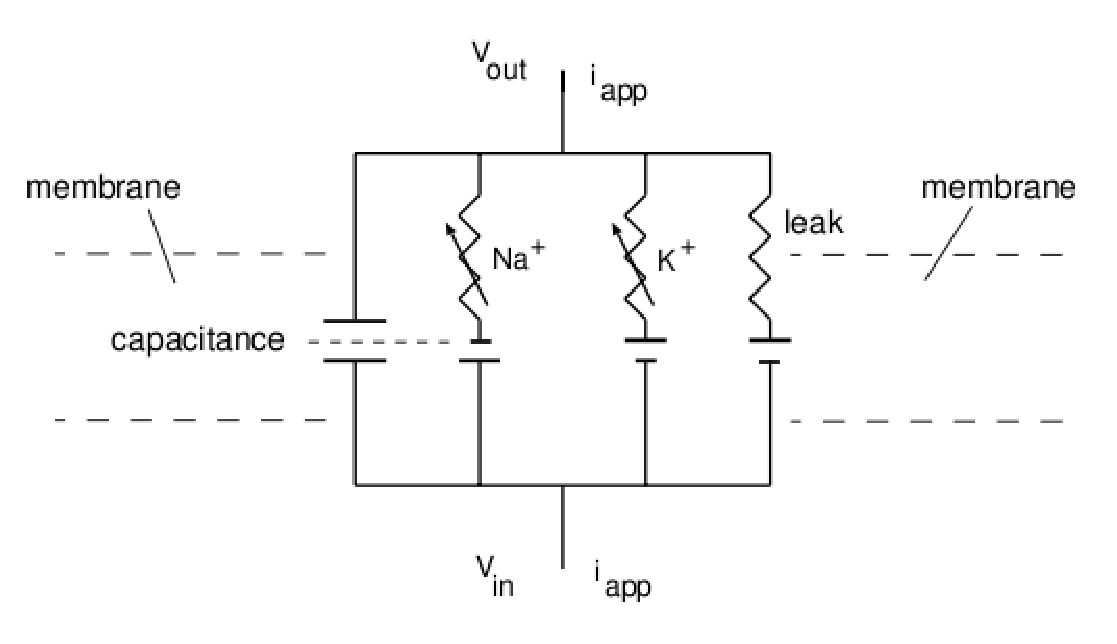
\includegraphics[height=5cm]{./images/Electric_Circuit_Membrane.eps}}
%   \caption{Equivalent circuit of biomembrane}\label{fig:membrane-circuit}
% \end{figure}
% As nerve cell is the subject of the study, the equivalent circuits to
% such part of the membrane originated by

% The resting potential in eq.~\eqref{eq:28} is a {\it steady state} in
% which each type of ion channels is permeable by only one specific type
% of ions. And the expression for the GHK potential is a general case,
% i.e. a steady state solution of a different kinetic equation for total
% current based on different assumptions about how ion cross the
% membrane.

{\bf QUIZZ}: Calculate the resting potential using the information
given in Fig.~\ref{fig:ion_concentration} and $g_{\ce{Na}} = 0.5\times
10^{-6}$ S, $g_{\ce{K}} = 10\times 10^{-6}$ S,
$g_{\ce{Cl}} = 2.5\times 10^{-6}$
S.

References: ~\citep{moreton1968acf}



\subsection{Barrier Model: Eyring Rate Theory}
\label{sec:eyring-rate-theory}
\label{sec:energy-barrier}

Barrier model assume the ion moving across the ion channel via binding at
multiple location along the channel pores. This is known as {\bf hopping
models}. The individual ions can then hop along the channel from one binding
site to the next, at each site with a given rate constant,
Fig.\ref{fig:barrier-model-ion-channel}.

\begin{figure}[htb]
  \centerline{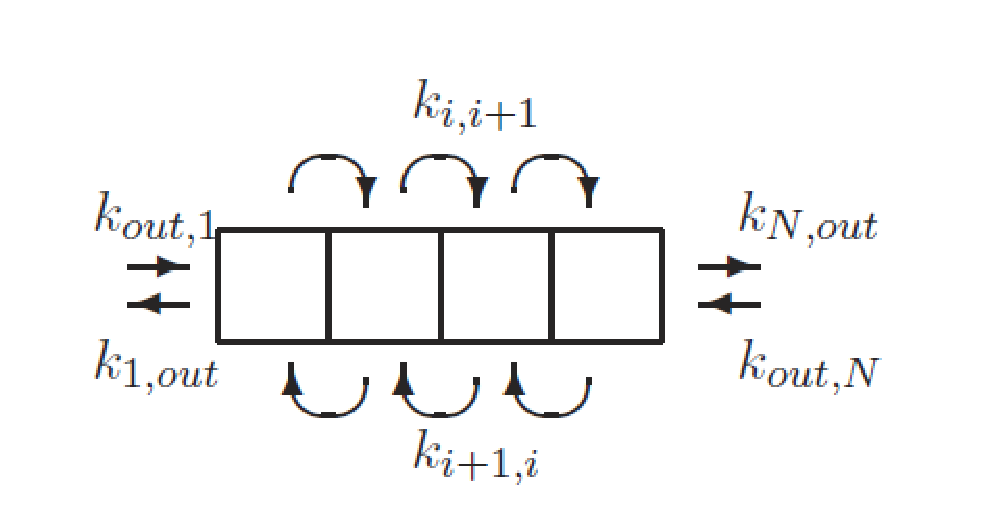
\includegraphics[height=3cm]{./images/barrier-model-ion-channel.eps}}
  \caption{Barrier model with multiple
  sites during ion movement}\label{fig:barrier-model-ion-channel}
\end{figure}

One standard approach for defining these hopping rates is to use
Arrhenius type rate constants
\begin{equation}
k_{i,j} = k_o \times \exp\left( - \frac{\Delta U}{k_BT} \right)
\end{equation}
with $\Delta U$ is the energy barrier a particle has to cross to jump to the next binding
site.  It is generally assumed that the energy barrier $\Delta U$ or $E_{ij}$
can be decomposed into two parts:
\begin{enumerate}
  \item protein-intrinsic potential landscape G that does not depend on the applied
membrane voltage

   \item the second part is contributed by a linear additive term that gives
the influence of the membrane voltage on the overall energy landscape
\end{enumerate}




The prefactor $k_o$ has been a subject of many discussions over the past
decades.
\begin{enumerate}
  \item The traditional prefactor: $k_o = \frac{k_BT}{h_p}$ where $h_p$ is
  Planck's constant

This is not species-dependent and has been considered inadequate in
since in a situation with no energy barriers present, all ion species would have
the same transition rates.

  \item Chen and his co-workers derive an alternative prefactor

\begin{equation}
k_o = \frac{D}{d^2} \frac{\exp(V_{appl}/(k_BT))}{\frac{1}{d} \int^d_0
\exp(\Delta U/(k_BT)) dx}
\end{equation}

with $V_{appl}$ is the applied external potential; $D$ = diffusion
coefficient and $d=	$ the width of the energy barrier.


Under the assumption of high energy barrier, then
\begin{equation}
k_o = \frac{2D}{d^2\sqrt{\pi}} \sqrt{|\frac{\Delta U}{k_BT}|}
\end{equation}
\end{enumerate}


\subsection{Poisson-Boltzmann model (PB)}
\label{sec:Poisson-Boltzmann-model}

In PB theory, the Poisson equation for the electrostatic potential V is
supplemented with the assumption that (at equilibrium) the distribution of
mobile ions can be approximated by the Botzmann factor

For small potentials V it is common to linearize this equation and one then
speaks of linearized Poisson-Boltzmann theory.

A comparison of PB with Brownian Dynamics simulations showed that the
PB approximation is inappropriate in the narrow channel geometry.

\subsection{Poisson-Nernst-Plank model (PNP): drift-diffusion systems}
\label{sec:Poisson-Nernst-Plank-model}

The macroscopic model based on the Poisson-Nernst-Planck (PNP) equations is used to
describe the transport of charged ions through a single open channel pore.

The underlying assumptions are that the ion movement through the pore is mainly
driven by diffusion and electrostatic interactions among the moving ions,
protein charges, and an externally applied electric field.

PNP is a mean field approach, i.e. time averages of the electrostatic field are
computed rather than the fluctuations on atomic time scales. So, it models
average charged densities of the ions instead of the movements of individual
ions. PNP approach is best used for relatively large channels like the L-type
Ca2+ channel or the ryanodine receptor that have a wider diameter of the
selectivity filter as e.g. compared to K+ channels.

\begin{mdframed}

The PNP equations have been used since decades as a standard model to describe
electro-diffusion in various systems, e.g. simulation of semiconductor devices.
The name drift-diffusion equations is another name for PNP system in physics.
In the ion channel context more species are included into the system (as
compared to only electrons and holes in semiconductor applications).

In 3D, it has a Poisson equation for the electrostatic potential V and a set of
continuity equations for the ion densities $\rho_k$.

The valence of each ion species is denoted by $z_k$ and the species-dependent
diffusion coefficient by $D_k$ (with $k$ represent $\Na$, $\K$ or $\Ca$).
Generally $D_k = D_k(x)$ is a space-dependent
function. The electrochemical potential $\mu_k$ can be decomposed into three
parts
\begin{enumerate}
  \item  the ideal part constituted by diffusion and mean field electrostatic
  interaction

  \item local short-range electrochemical interactions $\mu_k^{ex}$


  \item additional
externally applied potentials $\mu_k^0$
\end{enumerate}

The classical PNP approach ignores the short-range interaction terms and
additional external potentials. However, especially the first one will become
important when considering the restricted geometry of the selectivity filter. As
space is limited inside the filter region, crowding effects gain importance for
the proper determination of the particle densities.

\end{mdframed}

In 2D system of ionic diffusion, Fig.\ref{fig:PNP-2D-ionic-diffusion}, with the
measured current $I$ flowing through the channel from one bath to the other is
given by
\begin{equation}
I = e_o \int^{m-1}_{i=1} \int_{\Gamma_o}z_k J_k dn
\end{equation}
with $\Gamma_o \subset \Gamma_D$ constitutes one part of the Dirichlet boundary.

\begin{figure}[htb]
  \centerline{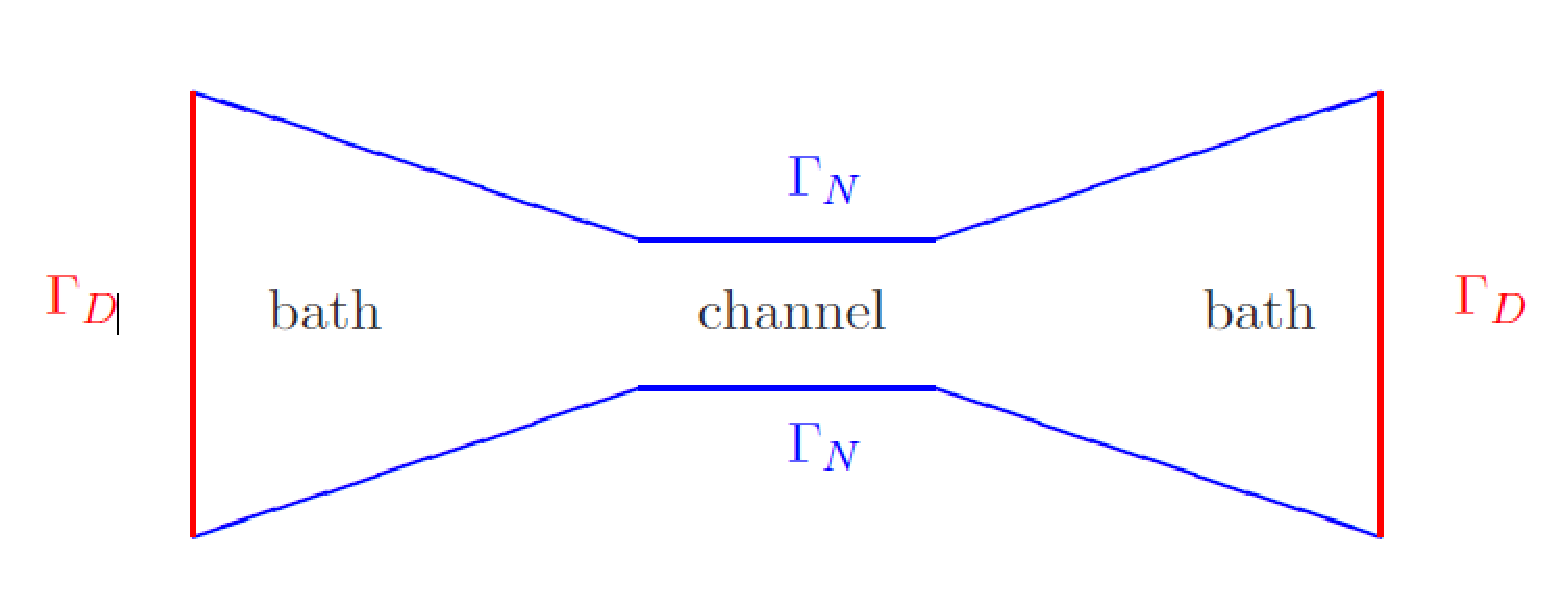
\includegraphics[height=6cm]{./images/PNP-2D-ionic-diffusion.eps}}
  \caption{PNP-2D-ionic-diffusion}\label{fig:PNP-2D-ionic-diffusion}
\end{figure}








Eyring rate theory is used to model the saturation of current at high
concentration of permeate ions \citep{lauger1973}. Some studies assumed no
more than one ion could occupy the pore at any one time. Such one-ion models
avoid concentration-dependent ionic permeability ratios and flux ratio exponents
of unity. So, only voltage-dependent can be accounted for \citep{hille1978,
lauger1973, begenisich1979}. Other studies have focused on multi-ion pores
\citep{hille1978, begenisich1979} that incorporate concentration-dependent
permeability ratios and flux ratio exponents of greater than one.

Because of mathematical simplicity, it's preferable to use one-ion model where a
single ion at a time can occupy the channel. In certain cases, like $\Ca$
channels, it cannot predict the saturation of calcium current with increasing
$[\Ca]_o$.  A better approach is combining Eyring rate theory
\citep{eyring1931,eyring1935,eyring1949} and standard chemical kinetics which
treat channels as a series of energy wells and energy barriers (See Appendix
\ref{sec:barrier-model}).

There are two parts we need to deal with: (1) the pre-exponential term and (2)
the activation energy part. {\bf Eyring equation} or Eyring-Polanyi equation
relates the reaction rate to
temperature\footnote{\url{http://en.wikipedia.org/wiki/Eyring_equation}}. The
original form is
\begin{equation}
k = \frac{k_BT}{h}\times e^{-\Delta ^\ddagger G}
\end{equation}
with $h$ is Planck's constant, $\Delta ^\ddagger G$ is the Gibbs energy of
activation [NOTE:
The symbol $\ddagger$ to indicate transition states (double dagger) is used as a prefix
to appropriate quantities, e.g. $^\ddagger G$, rather than the more often used
$\Delta G^\ddagger$] \citep{muller1994}. The pre-exponential part has been dealt
by different researchers (review:\citep{laidler1983}), before it came to the
above equation developed by Eyring in 1935, and at the same times Evans and Polanyi.
It is known as {\bf transition-rate  theory}.

Consider a channel with a number of binding sites, e.g. two binding sites,
reflected by local energy minimum flanked by symmetrical barriers, and that the
sites can be bind simultaneously. Transitions of ions between different states
of occupation can be described as rate constants $k$, which are
Voltage-dependent
\begin{equation}
k(V_m) = \frac{k_B T}{h}\exp\left( -\Delta ^\ddagger G/(RT) - z\delta V_m F/(RT)
\right)
\end{equation}
with $\delta$ is the fraction of the electrical field experienced by the ion
during the transition, $z$ is the valance. The term $k_BT/h$ represents the
intrinsic frequency of thermal vibration ($=6.5\times 10^{12}$ s$^{-1}$ at
22$^\circ$C), indicating the maximum value of the rate constants. The rate
contants for the transition of ions from the intra- (or the extra-)cellular to
the binding site has the same form, but multiplied by the
concentration of intracellular ion (or extracellular ion, respectively).
%Based on
% the collision theory of gases, where molecules are treated as hard spheres, C
% and B, the collision number $Z_{CB}$ (i.e. the total number of collision per
% unit time per unit volume) is
% \begin{equation}
% Z_{CB} = N_C N_B d^2_{CB}\left( 8\pi k_BT \frac{m_C+m_B}{m_Cm_B} \right)^{1/2}
% \end{equation}
% with $N_C,N_B$ are the total number of molecules of C, and B, respectively, per
% unit volume, $d_{CB}$ is the sume of the radii, $m_C,m_B$ are the masses. When $Z_{CB}$ is multiplied by
% the Arrhenius factor $e^{-E_a/(RT)}$, it gives the rate of reaction between A
% and B. Then, we take the division by $N_C N_B$, and multiply by the Avogadro
% number $N_A$, this returns the rate constant in molar unit (SI:
% m$^3$.mol$^{-1}$.s$^{-1}$)
% \begin{equation}
% k = N_A d^2_{CB} \left( 8\pi k_BT \frac{m_C+m_B}{m_Cm_B} \right)^{1/2}
% e^{-E_a/(RT)}
% \end{equation}
% This is however, not provide a good approximation to observed rates, and thus
% need refinement. A better approach using Maxwell-Boltzmann distribution, where
% Rice applied statistical analysis and came up with the formula
% \begin{equation}
%
% \end{equation}

\begin{mdframed}
  Each internal energy (inner/outer) well represents an ion-binding site
  and ions can interact by competing for these sites.
\end{mdframed}

\begin{figure}[hbt]
  \centerline{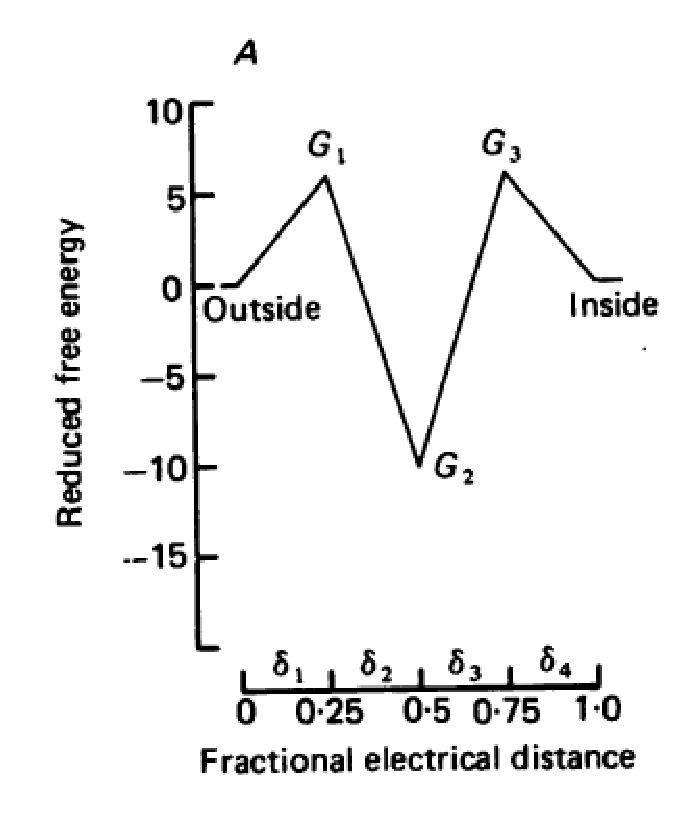
\includegraphics[height=5cm,
    angle=0]{./images/energy_well.eps}}
\caption{Energy well of single-binding site on each side}
\label{fig:energy_well}
\end{figure}

Example: The mechanism for transporting $\Ca$ ion across the channel with the
energy barrier as shown in Fig.\ref{fig:energy_well}. The channel has a single
binding-site with an energy barrier on either side.
The site can be empty (X) or occupied with calcium (XCa)

\begin{equation*}
  \begin{split}
    \ce{X + Ca <=>[k_1][k_{-1}] XCa <=>[k_2][k_{-2}] X + Ca} \\
    \text{(outside)} \;\;\;\;\;\; \;\;\;\;\;\; \;\;\;\;\;\; \;\;\;\;\;\; \;\;\;\;\;\;\text{(inside)}
  \end{split}
\end{equation*}
with the rate constants are exponential functions of the barrier
height and fractional membrane potential.
\begin{eqnarray}
  \label{eq:1041}
  k_1 = A.\exp\left(-G_1 -\delta_1z_\Ca V_mF/(RT) \right) \\
  k_2 = B.\exp\left(-G_3 + G_2-\delta_3z_\Ca V_mF/(RT) \right) \\
  k_{-1} = B.\exp\left(-G_1 + G_2-\delta_2z_\Ca V_mF/(RT) \right) \\
  k_{-2} = A.\exp\left(-G_3 -\delta_1 z_\Ca V_mF/(RT) \right)
\end{eqnarray}
with $G_1,G_3$ are the heights of the inner and outer energy barrier,
respectively. $G_2$ is the depth of the energy well. A is the average
vibration frequency for biomolecular reactions ($10^{11}$ sec$^{-1}$
molar$^{-1}$) and B is the average vibration frequency for solid
($10^{13}$ sec$^{-1}$). If the energy well was placed half of the
electrical distance through the membrane, we have
$\delta_1=\delta_2=\delta_3=\delta_4=0.25$. If we place the well close
to the inner membrane surface, we choose $\delta_1+\delta_2=0.75$.

The depth of the energy was selected so that it gives the $\Ca$
dissociation constant $K_\ca=7.3$mM in the absence of voltage field
($V_m=0$mV). Finally, the net flux through the channel in steady-state is given
\begin{equation}
  \label{eq:1042}
  J=\frac{k_{-1}k_{-2}[\Ca]_i-k_1k_2[\Ca]_o}{k_1[\Ca]_o+k_{-2}[\Ca]_i+k_{-1}+k_2}
  \;\;\; (\text{sec}^{-1})
\end{equation}
and the single channel current is
\begin{equation}
  \label{eq:1043}
  I = z_\Ca \times e \times J
\end{equation}
with $e = 1.6\times 10^{-19}$C (absolute value of the charge on electron).


{\bf Example 2}: \citep{vanHooft2003} with two binding sites and two permeable
ions ($\Ca$ and $\Na$). This gives 9 different occupation states. The fraction
of $\Ca$ current is
\begin{equation}
\frac{I_\ca}{I_\ca + I_\na}
\end{equation}
and the estimated permeability ratio $P_\ca/P_\na$ is
\begin{equation}
= \frac{[\Ca]_o}{[\Ca]_o + P_\na/P_\ca \times ([\Na]_o/4)\times \left[ 1 -
\exp(2V_mF/(RT)) \right]}
\end{equation}
Concentrations are converted to ion activities, with activity coefficients 0.5
for $\Ca$, and 0.7 for $\Na$.

{\bf Example 3}: Na models  (Sect.\ref{sec:Ina_Begenesich1980})


%  Ohm's
% law (Sect.\ref{sec:ohms-law}) cannot be used in most cases. Some of the
% biophysical laws use Nernst's equation (Sect.\ref{sec:nernst-equation}) or GHK
% equations (Sect.\ref{sec:GHK_current}).


\subsection{Deterministic movement of ions: molecular dynamics simulation with
Newtonian's law}

Molecular Dynamics (MD) is a method that is based on the atomistic details of a
system. MD really takes each individual particle (e.g. $\Ca$ ions) in the system
into account. It can thus be seen as the most detailed, but also as the
most complex method for simulation.

To model ionic conductance, MD takes into account individual $\Ca$ ions at the
extracellular and intracellular side; and every particle in the system behaves
according to Newton's laws of motion. It is thus a deterministic approach, since
for a given initial configuration the evolution of the system is determined by
Newton's law.

MD simulation consists of computing the trajectories of every particle in the
system, which is done by integrating Newton's second law
\begin{equation}
\frac{d{\bf x}^2}{dt^2} = \frac{\mathbf{F}}{\mathbf{m}}
\end{equation}
with the vector ${\bf x}$ represent the coordinates of all particles;
$\mathbf{F}$ the forces acting on every particle; and $\mathbf{m}$ the
mass of all particles.

One major issue in MD is the choice or the design of the force field $F$.
Ideally, all interactions between all the particles in the system should be
included, leading to a strongly coupled system of equations.
\begin{enumerate}
  \item First MD simulations (1957) was based on simple models done by Alder and
  Wainwright.

  \item Later, far more accurate and complex fields have been used.

  Software for MD simulations: AMBER, CHARMM and GROMOS/GROMACS, utilize
  prominent force fields that differ in certain parameter settings
\end{enumerate}
\textcolor{red}{The choice of time-step is critical}
\begin{itemize}

  \item  Too large timesteps lead to instabilities, since two particles
might have already crashed into each other during the long time step which
otherwise would have collided smoothly.

 \item Too small time steps: take too much time

 \item Leach (in the book: Molecular Modelling -  Principles and Applications,
 1996) suggests $10^{-14}$ seconds or $10^{-5}$ nanoseconds for (atom systems
 and translational motion); to $5\times 10^{-16}$ seconds for
 for flexible molecules with flexible bonds, when translation, rotation,
 torsion and vibration are present.

\end{itemize}

To generate a reliable flux, time spans of micro- to milliseconds have to be
simulated, while the range covered by MD simulations is currently on the time
scale of nanoseconds. From the numbers above we already see that it is difficult
to really simulate the ion transport through membrane channels using MD.

Nevertheless, with certain simplifications like potential of
mean force approximations of the solvent, MD might be used to get an idea of the detailed
picture e.g. from the protein residues lining the filter wall. However, setting up the force
field required for the simulation can pose several problems, especially in the case of synthetic
nanopores, since the conventional force fields for simulating biomolecular systems do not
include synthetic materials.



\subsection{Stochastic movement of ions: molecular dynamics simulation with
Langevin equation}

Models where the explicit solvent is replaced by some approximate model,
introducing random forces into the system, are also known as Stochastic or
Brownian Dynamics. There Newton's law of motion is replaced by the Langevin
equation that includes friction due to the solvent and some random fluctuations.

\subsection{Stochastic gating of ion channels:}

Another stochastic approach to determine the possible configurations of a system
are the so-called Monte Carlo methods.

Imagine a system consisting of N different particles whose coordinates
$\mathbf{r}^N$. The probability density of finding the system in configuration
$\mathbf{r}^N$ is determined by Boltzmann equation (Sect.\ref{sec:macr-state-vs})
\begin{equation}
\frac{\exp\left( -\beta \mathcal{U}(r^N)\right)}
{\int \exp\left( -\beta \mathcal{U}(r^N)\right)}
\end{equation}
with $\mathcal{U}$ denotes the energy of the system, and $\beta =
\frac{1}{k_BT}$. The Boltzmann factor is the exponential term.

The MC helps to determine the equilibrium distribution of ions inside the
channel.
\begin{enumerate}
  \item In {\bf importance sampling}:  the probability of visting a particular
  point $r^N$ of the configuration space is proportional to the Boltzmann factor

  \item In {\bf random sampling}: the configuration points are distributed randomly
over the whole phase space
\end{enumerate}
The importance sampling on the other hand focuses on regions of the phase space
that have an important contribution to the ensemble average.

Metropolis et al. in introduced a method for importance sampling  and the
resulting method is hence called the Metropolis MC method. It is nowadays
widely-used in MC simulations, to efficiently sample the phase space.
\begin{enumerate}
  \item given an initial configuration of the system $r^N$, compute the energy
  $\mathcal{U}(r^N)$; then

   \item at each time step: only allow 1 particle to move.

   This can be done by (1) select a particle at random, (2) generate a movement;
   (3) check if we accept the move or not.

  \item step (1) + (2)

   So, we select a particle at random, and give it a random placement
   $r' = r + \Delta$. With this, calculate the resulting energy
   $\mathcal{U}{r'^N}$

  \item step (3): the acceptance of the move is given by the probability

  \begin{equation}
  p_{acc} = \min\left\{ 1, \exp(-\beta \left[ U(r'^N) - U(r^N) \right])
  \right\}
  \end{equation}
  NOTE: $p_{acc} = 1$ when the enegy decreases, i.e. the move is always accepted if it does not lead to an increase in
the energy.

  To do so, generate a random number $c$ from a uniformly distributed [0,1]; if
  the random number if less than $p_{acc}$, then accept the move; otherwise, the
  move is rejected and the old configuration is kept for the next step.

\end{enumerate}


In order to get an efficient algorithm the displacement $\Delta$ has to be
chosen appropriately. If it is chosen too large, the moves are rejected too
often and little movement through the phase space is achieved.
On the other hand, if the displacement is chosen too small there is
a high acceptance rate for the moves but the phase space is explored slowly
anyway




\section{Rectification: outward-rectification, and inward-rectification}
\label{sec:rectification}


{\bf Rectification} means the change of conductance due to the two opposing
forces
\begin{itemize}
  \item the membrane potential $(\Vm - E_\rev)$

Under symmetric concentration condition, in Ohm's law, the linear
function of voltage gradient across the membrane is the driving force for the
ionic current, e.g. I=g(V-E); and the I-V curve would be a straight line passing
through the origin, i.e. $E = 0$ (mV).

So, if $\Vm > E_\rev$: it drives the inward current.
%\ref{sec:calcium-dynamics}
  
  \item the concentration gradient of the permeable ions, which 
  has unequal ion concentration across the biomembrane.

In the case of $\K$, as $[\K]_i > [\K]_o$, it drives the current in the outward
direction.

\end{itemize}
So, the balance of this two driving forces can change the direction of the
overall current through that ion channel.

When current flows more easily from a side of high permeant ion
concentration, this form of rectification is called {\bf Goldman-Hodgkin-Katz}
rectification (or open rectification) - Sect.\ref{sec:GHK-rectification}.


Channels can rectify if they only open in a voltage range that favours outward
or inward current
\begin{itemize}

  \item {\bf Outward rectification} means the outward current is more stronger
  upon transmembrane potential changes.

Most potassium outward currents open with a delay after the transmembrane
voltgage change, thus they are called {\bf delayed outward rectification}
(Sect.\ref{sec:delayed-rectifier}).

Some voltage-gated K+ channels show voltage-dependent outward rectification
because they open only with membrane potential value at which outward K+
flux is favoured.


  \item {\bf Inward rectifier} : e.g. Sect.\ref{sec:K+-inward-rectifier}

Some depolarization-activated channels are inward rectifiers because they
inactivate so rapidly once they open that they only pass large currents on
recovery from inactivation at negative voltages where inward flux is favoured.

Still other voltage-gated channels show inward rectification because they are
opened by steps to hyperpolarized voltages.

Some channels rectify because they are blocked in a voltage-dependent fashion.
Example: inward rectifiers of the Kir class allow for the passage of inward
current because internal magnesium and polyamines obstruct them when membrane voltage is
positive to EK. The channels are unblocked at hyperpolarized potentials below EK,
allowing significant inward K+ flux (Sect.\ref{sec:Kir_family}).

Remember that when a channel opens, the ion flows independently in both
directions. So, {\bf inward rectification} means that given an equal, but
opposite electrochemical driving force; the inward flow exceeds the outward
flow.

% the inward current is stronger upon transmembrane potential changes
\end{itemize}


\subsection{GHK rectification (open rectification)}
\label{sec:GHK-rectification}
\label{sec:open-rectification}

What GHK rectification means is that:
\begin{itemize}
  \item KCNK0 currents change in a linear fashion as a function of voltage
when the K+ concentration is identical across the membrane

  \item But when the concentration of K+ is high intracellularly and low
  extracellularly, a larger outward current is observed
\end{itemize}
In GHK's equation, it is assumed that the  ions move independently of each
other, and the total flow of ions across the membrane is simply equal to the sum
of two oppositely directed fluxes.

Potassium channels preferentially pass current in one direction.
Most, if not all, ion channels show some degree of open rectification.
\textcolor{blue}{The degree of rectification is dependent on the concentration
gradient: the greater the concentration gradient, the greater the
voltage-dependent current rectification}. This phenomenon is well described by
the Goldman-Hodgkin-Katz (GHK) current equation (Goldman, 1943; Hodgkin and
Katz, 1949; Hodgkin and Horowicz, 1959).


\section{Pump-Leak model: Leakage channels (leak current)}

The size of the needed ionic flux to balance the model depends on the surface
area of the cell; whereas the effect of the ionic flux on the internal
concentrations depends on the volume of the cell. To balance a model, there are
always active fluxes which use energy and passive flux which depends on chemical
gradients. This passive flux forms a constant background current, regardless of
the different ion channels incorporated into the computational model or how
selectivity of the sarcolemma membrane (SL). These 'unknown' channels are called
{\it leakage} channels of the membrane.

% , there is always a small little
% current to affect the resting potential, which seems to form a constant
% 'background' current.
% However, with this leakage current, in the end, everything will be in equal, and
% the cell will be exploded. To avoid this problem, a mechanism known as active
% pump exist to stop the run down in concentration gradient.

There are different types of pumps, e.g. $\Na/K$ exchange pump. Active pumps use
metabolic energy obtained by hydrolizing ATP to pump $\Na$ and $\K$ ions against
their concentration gradients (Na:K=3:2, with 3Na out in exchange for 2K in) to
balance the passive flux. Active pumps will be covered in Chapter
\ref{chap:models-pumps}.

The transport ratio $r$ (e.g. r=1.5 for Na/K exchanger) of the active pump has
the reversal potential
\begin{equation}
E_\rev = \frac{RT}{zF}\log \frac{r[\K]_i + \alpha [\Na]_i}{r[\K]_o + \alpha
[\Na]_o}
\end{equation}
In squid giant axon, Na/K exchange pump makes a small contribution ($\approx
-4$mV) to the resting membrane potential.

\section[Solving Electrical Property of Biomembrane]{Examples: Solving
Electrical Property of Biomembrane}
\label{sec:exampl-ionic-curr}

\subsection{Simple system with one type of ionic channel}

As mentioned in Sect.~\ref{sec:introduction}, the example in
Sect.~\ref{sec:model-ion-channel} utilized 3 assumptions.
\begin{enumerate}
\item Again, we assume there is one type of ion channels in the
  cell. For simplicity,
  \textcolor{green}{we examine the case when I-V is linear, or the
    current follow the simple Ohm's law}
  (Sect.~\ref{sec:ohms-law}), with the permeability is now replaced by
  conductances $g_i$, the current is
  \begin{equation}
    \label{eq:1413}
    I_i = g_i (V_m-E_i) \;\;\; \text{($\muA$)}
  \end{equation}

  So, what we need is to find $g_i$. At whole-cell level, the
  conductance is not constant, but proportional to the fraction of open
  channels $f_i$.

  \begin{equation}
    \label{eq:34}
    g_i = f_i \overline{g_i}
  \end{equation}
  with the maximum possible conductance is denoted as $\overline{g_i}$
  (g-bar).

\item Again, we assume the ion channel has 2 states:
  $\ce{C <=>[k^+][k^-] O}$. Reuse eq.~\eqref{eq:254}, the fraction of
  channel in each state is defined as
  \begin{equation}
    \label{eq:257}
    \frac{df_i}{dt}  =  - (k_i^-+ k_i^+) (f_i - \frac{k_i^+}{k_i^-+ k_i^+})
  \end{equation}
\end{enumerate}

{\bf Situation 1}: If the rate transition $k^+_i, k^-_i$ are all constant,
it was covered in Sect.~\ref{sec:model-ion-channel} of the previous chapter. For
a multiple channels system, we discuss it in Sect.\ref{sec:solv-electr-prop}.


{\bf Situation 2}: If the rate transition $k_i^-, k_i^+$ can change,
e.g. voltage-dependent. Thus, we may need ODEs for $k^+_i$ and
$k^-_i$. This case, though more complicated, is more realistic. We'll
examine in Sect.\ref{sec:example_Vm-gating-channel}.

\subsection{Simple system with multiple types of ionic channels}
\label{sec:solv-electr-prop}

Under the assumption of I-V relationship is linear (discussed in
Sect.\ref{sec:equat-ionic-curr}), the total conductance in a parallel circuit is
the sum of component conductance.

\begin{equation}
  \label{eq:51}
  g = \sum_i g_i
\end{equation}
When all ion channels are closed, the conductance is zero. For a
single type of ion channels $i$, the conductance should be
proportional to the fraction of open channels $f_i$. If
all channels $i$ are active (open), the maximum possible conductance
is denoted as $\overline{g_i}$ (g-bar). If at a single time point, given
the fraction of open channels as $f_i$, we have

% the total conductance $g_i$ is the product of the $\overline{g_i}$ and

In the simple case, when the biomembrane has only one type of ion
channels with reversal potential $E_{rev}$, then the relation of the
current flows is
\begin{equation}
  \label{eq:35}
  \Csc \frac{dV_m}{dt} =  -f\overline{g} \times (V_m-E_{rev}) + I_\app
\end{equation}

\textcolor{green}{It is normally assumed that the leak conductance never
  change, $g_{\leak}=\overline{g}_{\leak}$}.
Finally, eq.~\eqref{eq:33} is equivalent to
\begin{equation}
  \label{eq:52}
  \Csc \frac{dV_m}{dt} =  -f_K\overline{g_K} \times (V_m-E_{\ce{K}})
  -f_{Na}\overline{g_{Na}} \times (V_m-E_{\ce{Na}})+ \overline{g_{\leak}} \times (V_m-E_{\leak}) + I_\app
\end{equation}
with $\overline{g_i}$ are constants and can be determined experimentally,
$E_i$ are reversal potential for channel $i$; $f_i$ are fraction open
channels, i.e. time-dependent quantities.  As $E_{leak}$ can be easily
taken out from the formula, i.e. define $V_m$ as $V_m-E_{leak}$ and
$E_i$ as $E_i-E_{leak}$.
\textcolor{red}{For simplicity, $E_{\leak}$ is assumed to be zero}.
\begin{equation}
  \label{eq:929}
  \Csc \frac{dV_m}{dt} =  -f_K\overline{g_K} \times (V_m-E_{\ce{K}})
  -f_{Na}\overline{g_{Na}} \times (V_m-E_{\ce{Na}})+ \overline{g_{\leak}} \times V_m + I_\app
\end{equation}

Thus, problem in eq.~\eqref{eq:33} has been mapped to
eq.~\eqref{eq:929}. To solve this differential equation, we need to
know the fraction of open channels $f_i$ which are time-variant quantities.


To solve eq.~\eqref{eq:33}, we need to know
\begin{enumerate}
\item $I_\app$: stimulus current ($\mu$A/cm$^2$), can be controlled
\item $E_i$: reversal potential [mV] for channels of type $i$, can be
  determined experimentally (using antagonists to turn off all other
  ion channels, and then measure channels of type $i$ in isolated at
  rest)
\item $\Csc$: specific membrane capacitance ($\mu$F/cm$^2$) -
Sect.\ref{sec:specific-membrane-capacitance}).

\item $g_i$: (mS/cm$^2$) a time-dependent quantity (has complicated
  kinetics and need to formulate properly using mathematical tools). Here, we
  model simply $g_i = f_i \overline{g}_i$ with $\overline{g}_i$ is the maximum conductance
  which can be measured experimentally.
\end{enumerate}


{\bf NOTE}: For a single type of channel, at steady state, when there is no
change in membrane potential, the left side of eq.~\eqref{eq:35} should be zero.
 The fraction of open channel is $f_\infty$ and the steady state membrane
potential is now
\begin{equation}
  \label{eq:151}
  V^{ss} = E_{rev} + \frac{I_\app}{f_\infty\overline{g}}
\end{equation}

{\bf QUIZZ}: A proto-cell has a specific membrane capacitance
$\Csc=1\mu$F/cm$^2$ and contains only \ce{K+} selective channels, with initial
concentration (inside and outside) as given in Fig.~\ref{fig:ion_concentration}.
Besides \ce{K+} ions, there are also anions \ce{A-} equal in concentration to
\ce{K+} at both cytoplasmic and extracellular environment.

\begin{enumerate}
\item If \ce{K+} channels open, what is the steady state voltage
  across the membrane, assuming ion concentration do not change? --
  Using eq.~\eqref{eq:151} and  $I_\app = 0$.

\item How many \ce{K+} must move out of the cell per cm$^2$ to achieve
  a voltage difference equal to that in part (1)
\end{enumerate}


% Using eq.~\eqref{eq:35}, it is possible to estimate the {\it
%   characteristic time for the relaxation of the membrane
%   potential}. When all channels are open, then $f_i=1$, and
% \begin{equation}
%   \label{eq:142}
%   \frac{dV_m}{dt} =  - \frac{(V_m-E_{rev})}{\hat{\tau}} + I_\app/C
% \end{equation}
% with the estimated characteristic time is
% \begin{equation}
%   \label{eq:87}
%   \hat{\tau} = C/\overline{g}
% \end{equation}

% {\bf NOTE}: The role of relaxation time, the higher the value of
% $\hat{\tau}$, the slower the change in membrane voltage.


\subsection{More complicated system where channels are $V_m$-gated}
\label{sec:example_Vm-gating-channel}

% \subsection{Finding $g_i \leftrightarrow f_i \leftrightarrow V_m$}
% \label{sec:g_i-rightl-f_i}

% \subsubsection{Important notice}
% \label{sec:important-notice}

% So far, the transaction rate from one state to another is assumed to
% be constant.
This section continues the analysis of the previous section, under the
assumption that either or both $k^+_i, k^-_i$ are
voltage-dependent. Thus, $k^+$ should be a function of $V_m$; then the
fraction of open channels $f_i$ should be a function of membrane
voltage $V_m$, i.e. $f_i(V_m)$. So, from the relation between $g_i$
and $f_i$, we can build the relation between $g_i$ and $V_m$.


A better form of eq.~\eqref{eq:257} is in the {\bf first-order form}
\begin{equation}
  \label{eq:36}
  % \frac{df_0}{dt} = -\frac{f_0-f_\infty}{\tau}
  \frac{df_i}{dt} = -\frac{f_i-f_{i,\infty}}{\tau_i} =
  \frac{f_{i,\infty} -f _i}{\tau_i}
\end{equation}
with
\begin{equation}
  \label{eq:37}
  f_{i,\infty} = \frac{k_i^+}{k_i^++k_i^-}, \tau_i = \frac{1}{k_i^++k_i^-}
\end{equation}
are called the {\it steady state} open fraction and the characteristic
mean open {\it time constant} (aka {\it relaxation time constant})
(Sect.~\ref{sec:how-fast-reaction}), respectively. The unit
$[f_\infty]$ = unitless, $[\tau]$= sec$^{-1}$. For a reaction at equilibrium,
\begin{equation}
[\Ca] + [\text{Buffer}] \ce{<=>} [\text{Ca.Buffer}]
\end{equation}
the time constant is estimated as
\begin{equation}
1/\tau = k^+ [\text{Buffer}_{total}]
\end{equation}


\textcolor{blue}{For simplicity in notation, the index $i$ is
  neglected.}
$k^+, k^-$ are time-variant quantities that represent
the rates of transition $\ce{C}\ce{<=>[k^+][k^-]}\ce{O}$.

% In order to solve the linear ODE in eq.~\eqref{eq:52} and
% eq.~\eqref{eq:257}, we still need to know the rate constants $k_i^-,
% k_i^+$.
% % Later, you will know that the two quantities $f_{\ce{K+}},
% % f_{\ce{Na+}}$ are voltage-dependent.
\begin{figure}[hbt]
  \centerline{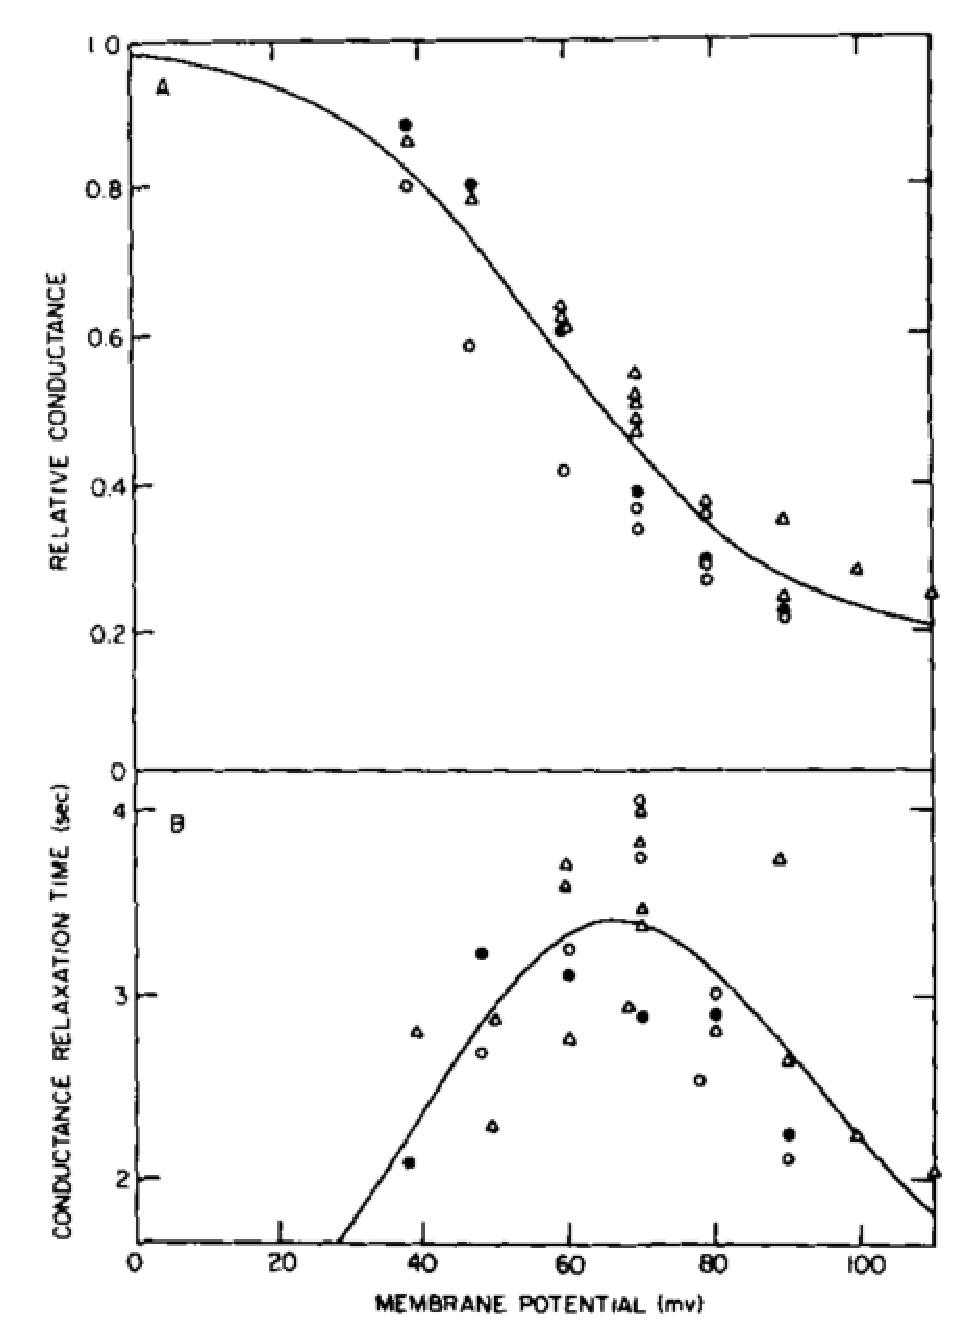
\includegraphics[height=7cm,
    angle=0]{./images/Lecar_g_V.eps}}
  \caption{Normalized $V_m$-dependent conductance and conductance
    relaxation time for a protein extracted from aerobacter bacteria}
  \label{fig:Lecar_V_g}
\end{figure}

\begin{equation}
  \label{eq:79}
  f_{\infty} = \frac{k^+}{k^++k^-}, \tau = \frac{1}{k^++k^-}
\end{equation}
Interestingly, experimental
  results~\citep{lecar1975mcg} shown that the fraction of open
  channels $f$, is a sigmoid function of voltage $V_m$, and the
  relaxation time constant $\tau$ is a bell-shaped function of voltage
  $V_m$,
Fig.~\ref{fig:Lecar_V_g}. This means that \textcolor{red}{there's a biphasic
bahavior of ion channel gating where the conductance-$V_m$ follows a nice bell-shaped
relationship}. Up till now, this still serve as the basic for building kinetic
models of voltage-gated ion channels. The next section will provide some
numerical result to prove this.

\subsection{-- f($V_m$)}
\label{sec:fv_m}

Given that f($V_m$) is a sigmoidal function of $V_m$, the question is what is a
proper functional form of $f(V_m)$. Assuming that each state (Open or Close)
corresponds to a major conformation of the channel which is associated with a
particular level of potential energy, as shown in Fig.~\ref{fig:state_energy},
in which the transition from one state to another need to overcome a threshold
activation energy.

% The probability for the channel to be at a given state is given by the
% Gibbs  energy change $E_i$ which is a function of the internal
% electrostatic and Van der Waals interaction between protein residues,
% entropy of protein folding, and external electric field. This
% probability follows the so-called Boltzmann distribution.
% \begin{equation}
%   \label{eq:690}
%   Prob(E_i) = \frac{\exp{-\frac{E_i}{k_BT}}}{\sum_j\exp{-\frac{E_j}{k_BT}}}
% \end{equation}
Based on Maxwell velocity distribution law, eq.\ref{eq:1333},
the probability for the channel to be at a given state is given by
\begin{equation}
  \label{eq:690}
  Prob(E_i) = \frac{\exp{-\frac{E_i}{k_BT}}}{\sum_j\exp{-\frac{E_j}{k_BT}}}
\end{equation}
where the activation energy $E_i$ is a function of the internal
electrostatic and Van der Waals interaction between protein residues,
entropy of protein folding, and external electric field. This
probability follows the so-called Boltzmann distribution.


\begin{figure}[hbt]
  \centerline{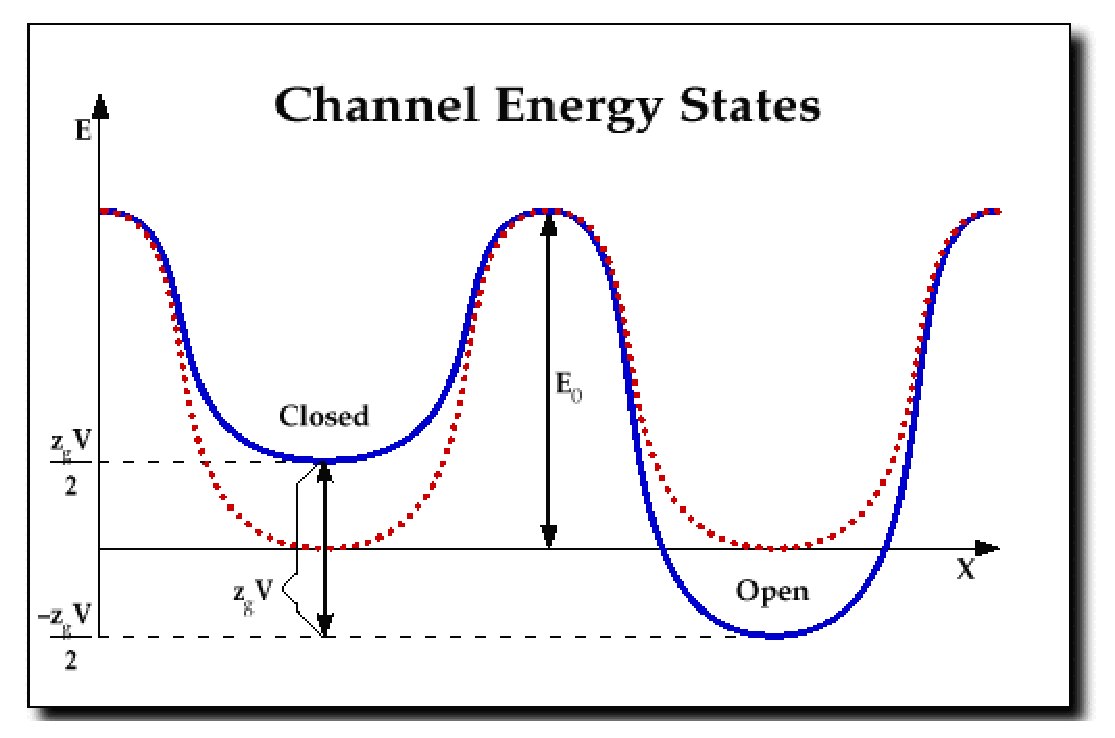
\includegraphics[height=5cm,
    angle=0]{./images/state_energy.eps}% ,
    % \includegraphics[height=5cm,
    % angle=0]{./images/channel_state_transition.eps}
  }
  \caption{State and energy}
  \label{fig:state_energy}
\end{figure}


\label{sec:Kramer-reaction-rate-theory}
At equilibrium, dotted red line in Fig.~\ref{fig:state_energy}, even though the
two state have the same energy, there is a rate that channels switch the state.
This is known as the {\bf Kramer's escape rate} across the activation energy
barrier
\begin{equation}
  \label{eq:691}
  r=\frac{D}{2\pi k_BT} \sqrt{E''(x_{min})|E''(x_{max})|}\exp(-\frac{E_0}{k_BT})
\end{equation}
with $x$ is the reaction coordinate, $E''(x_{min}),|E''(x_{max})|$ are
the curvature of the blue curve, i.e. when the magnitude of energy
difference between the two state is maximum, $E_0=|E(x_\max)-E(x_\min)|$.
\textcolor{red}{Assume that the change in energy in each state when
  changing the voltage is in opposite sign}
(i.e. never both state increase the energy simultaneously, which is like a
see-saw). Thus, regardless of the complicated energy calculation if we take
into account all factors affecting the activation energy of the ion channel,
the energy difference between the two states can be accounted for the
difference in conformational energy $W$ and the energy change $-zV_m$
due to the movement of the effective gating charge $z$ across the
membrane potential $V_m$. In other words, we can assume the energy difference to
be proportional to the voltage, i.e. $\Delta E=W-zV_m$.
NOTE: $z$ depends on the position of the positive charges in the S4
segment\footnote{S4 segment is the one that is the voltage-sensor in may ion
channels}, and the structure of the electric field within the membrane.
Thus, changing the membrane voltage may change the energy level at two
states, Fig.~\ref{fig:state_energy} which can lead to the more
likelihood of one state jumping to
another or vice versa\footnote{Read Chapter 7 of Thermo-Stat book}.

On a single cell membrane, experimental results have shown that
$\log(k^+)$, $\log(k^-)$ are linear functions of membrane voltage
$V_m$~\citep{ehrenstein1974koa}. So, the rate transition from one state to
another can be defined as
\begin{equation}
  \label{eq:692}
  \begin{split}
    k^+(V) = r \exp[-(\frac{W_1-zV_m}{k_BT})] \\
    k^-(V) = r \exp[+(\frac{W_2-zV_m}{k_BT})] \\
  \end{split}
\end{equation}
with $k^+(V)$ is rate from C to O, $k^-(V)$ is rate from O to C.  $r$
is an empirical factor (aka {\it coefficient of rate constant}) that
tells how often the voltage pass the threshold and is independent of
$V_m$.  Under the same experimental condition, the rate constant $r$
varies from membrane to membrane by an order of magnitude.

% At macroscopic scale, the movement of ions through thousands of ion
% channels, given the fraction of open channels is $f$, then
% \begin{equation}
%   \label{eq:693}
%   \frac{df}{dt} = k^+(V)\times[1-f]-k^-(V)\times f
% \end{equation}

If we assume that at $V_m=0$, all the
channels are open and the conductance is at
maximum~\citep{ehrenstein1970nnr}, then a simpler form for
eq.~\eqref{eq:692} is

\begin{equation}
  \label{eq:39}
  \begin{split}
    k^+ &= k_0^+ \exp(-\alpha V_m) \\
    k^- &= k_0^-  \exp(-\beta V_m)
  \end{split}
\end{equation}
with $\alpha, \beta$ are some constants (can be determined
experimentally) whose units are $\frac{1}{[\text{voltage}]}$. This
follows the Boltzmann distribution.

\subsection{-- Derive  $f_\infty$ and $\tau$}
\label{sec:analyze-f-tau}


Substitute them into eq.~\eqref{eq:79}, the new form of the steady
state fraction of open channels and the characteristic relaxation time
constant are
\begin{equation}
  \label{eq:40}
  \begin{split}
    f_\infty &= \frac{1}{1+\frac{k_0^-}{k_0^+}
      \exp((\alpha-\beta)V_m)} \\
    \tau &= \frac{1}{k_0^+\exp(-\alpha V_m)} \times \frac{1}{1+\frac{k_0^-}{k_0^+}\exp((\alpha-\beta)V_m)}
  \end{split}
\end{equation}
To make the expression more intuitive, we define
\begin{equation}
  \label{eq:42}
  S_0 = \frac{1}{\beta-\alpha}, \;
  V_0 = \frac{\ln (\frac{k_0^-}{k_0^+})}{\beta-\alpha}
  % \begin{split}
  %   S_0 &= \frac{1}{\beta-\alpha} \\
  %   V_0 &= \frac{\ln (\frac{k_0^-}{k_0^+})}{\beta-\alpha} \\
  % \end{split}
\end{equation}
with $S_0$ and $V_0$ are in unit of (Voltage).

Then, the new expression for the steady state fraction of open channel
and mean open time constant in eq.~\eqref{eq:40}, are
\begin{equation}
  \label{eq:43}
  \begin{split}
    f_\infty &= \frac{1}{1+\exp(-\frac{V_m-V_0}{S_0})} \\
    \tau &= \frac{\exp(\alpha V_m)}{k_0^+(1+\exp(-\frac{V_m-V_0}{S_0}))}
  \end{split}
\end{equation}
As given in the previous figure, $f_\infty$ should be a sigmoidal function of
$V_m$, and $\tau$ is the bell-shaped function with $V_m$
\textcolor{blue}{The curves are characterized by a slope
  factor $S_0$ and a half-point for the curve $V_0$. The potential
  $V_0$ is determined so that $f_\infty=0.5$}.


{\bf NOTE}:
\begin{eqnarray*}
  tanh(x) = \frac{e^{x}-e^{-x}}{e^{-x}+e^{x}}, cosh(x) = (e^{-x}+e^{x})/2
\end{eqnarray*}

Then, the {\it hyperbolic form} for those two expressions in
eq.~\eqref{eq:43} are
\begin{equation}
  \label{eq:45}
  \begin{split}
    f_\infty &= 0.5 \left( 1 + tanh (\frac{V_m-V_0}{2S_0})\right) \\
    \tau &= \frac{\exp(V_m\frac{(\alpha+\beta)}{2})}{2\sqrt{k_0^+k_0^-}cosh(\frac{V_m-V_0}{2S_0})}
  \end{split}
\end{equation}
with $S_0, V_0$ are given in eq.~\ref{eq:42}.

{\bf QUIZZ}: Prove the correctness of eq.~\eqref{eq:45}.

{\bf QUIZZ}: What is the meaning of $V_0$ and $S_0$? - To answer this,
you have to perform the below analysis. [ANSWER: $S_0$ is the membrane
potential at which half of the channel open, and $V_0$ is the slope of the
change (how fast/slow channels open: the higher $S_0$ in magnitude the faster
the change) and the sign of $S_0$ tells the sigmoidal is forward or backward].

\subsection{-- Analysis of $f_\infty$}
\label{sec:analysis-2}

To see how the values of $V_0$ and $S_0$ affect the fraction of open
channels, we examine two cases:
\begin{itemize}
\item  $V_0 = -50$mV, $S_0 = -2$mV
\item  $V_0 = -25$mV, $S_0 = 5$mV
\end{itemize}
The membrane potential $V_m$ is examined in the range from -75mV
(resting potential) to 25mV.

{\bf R-code}: \hyperref[chap2.1.r]{chap2.1.r}



\begin{figure}[htb]
  \centerline{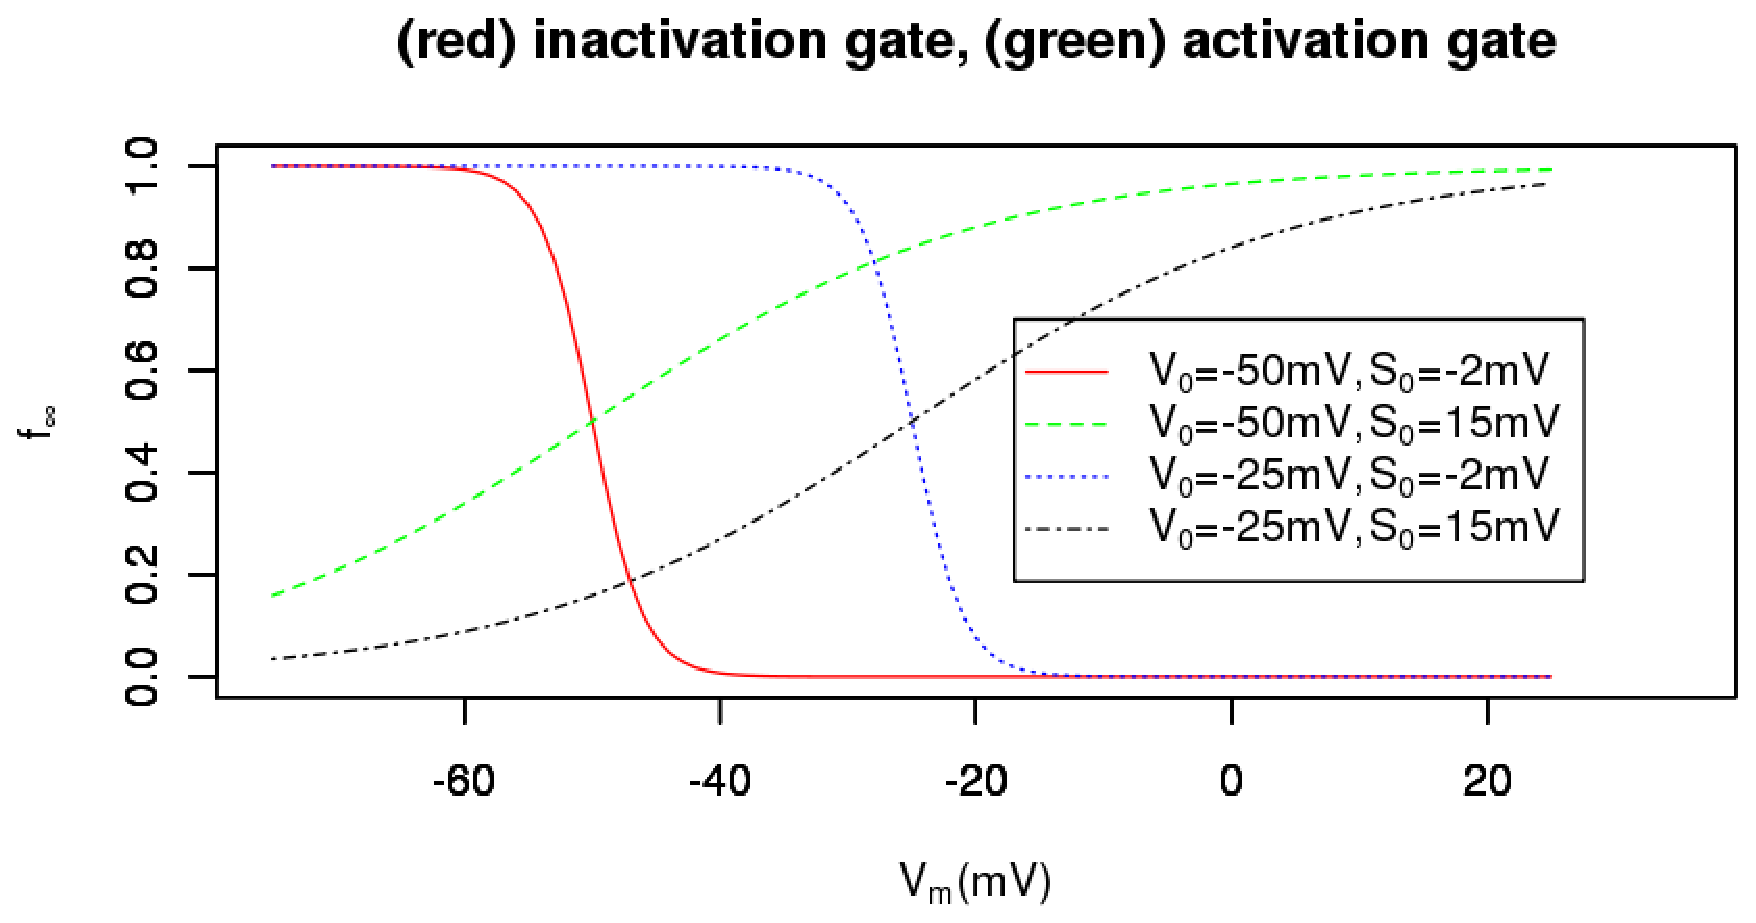
\includegraphics[height=7cm]{./images/equilibrium_open_fraction.eps}}
  \caption{Steady-state fraction of open channel (sigmoid function of
    $V_m$)}\label{fig:open_fraction}
\end{figure}

{\bf REMARK}:
\begin{itemize}
\item the activation is a sigmoid shape (green and black)

\item the inactivation is the reversed sigmoid shape (red and blue).

\item $V_0= \frac{\ln (k_0^-/k_0^+)}{\beta-\alpha}$ is the potential
  value that determines (1) half of the channel open at steady-state,
  (2) how early a channel is activated.

  With (2), it means that the ion channels with more negative $V_0$
  activate earlier than other ion channels during voltage
  depolarization. The gradually increasing in the sigmoid shape is
  interpreted as there is a multistep process in gating mechanism
  (will be discussed in the Hodgkin-Huxley's model)

\item the sign of $S_0 = \frac{1}{\beta-\alpha}$ tells us the trend of
  of channel gating following the membrane voltage. Initially,
  \begin{itemize}
  \item $S_0>0$: all gates close
  \item $S_0<0$: all gates open
  \end{itemize}
  Then, when the membrane potential depolarizes,
  \begin{itemize}
  \item In the case of $S_0>0$: gates tend to open
  \item In the case of $S_0<0$: gates tend to close.
  \end{itemize}
\item $S$ is the slope factor
  % \item the magnitude of $S_0$ inversely determines how fast the rate of
  %   state transition, i.e.  switching from open to close or vice
  %   verse. By looking at the steepness of the curve $f_\infty(V_m)$,
  %   i.e. the higher $|S_0|$ the less steepness. The lower steepness is
  %   considered as a delay (sigmoid shape). This sigmoidicity is
  %   interpreted as there is a multistep process in gating mechanism
  %   (will be discussed in the Hodgkin-Huxley's model)
\end{itemize}


\subsection{-- Analysis of $\tau$}
\label{sec:analysis}

$\tau$ is the mean open time. Here, the relationship between the membrane
potential $V_m$ and the exponential time constant $\tau$ is examined.  In our
case, the change in energy in each side is in opposite sign, as shown in
Fig.~\ref{fig:energy_profile}, thus we have

\begin{equation}
  \label{eq:53}
  \alpha = -\beta;
\end{equation}

\begin{figure}[hbt]
  \centerline{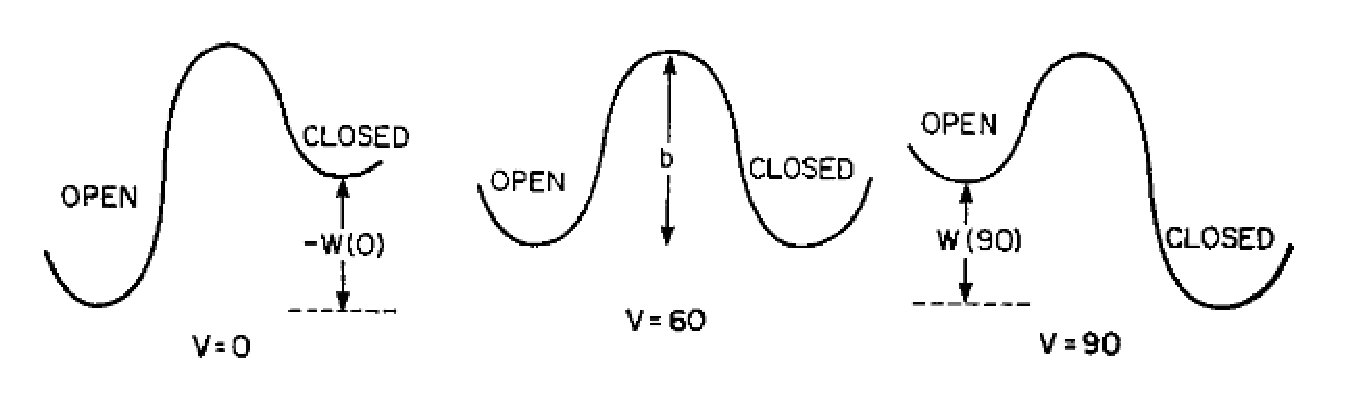
\includegraphics[height=3cm]{./images/energy_configuration.eps}}
  \caption{Energy barrier profile }
  \label{fig:energy_profile}
\end{figure}

Rewritten eq.~\eqref{eq:39}
\begin{equation}
  \label{eq:58}
  \begin{split}
    k^+(V_m) &= k_0^+ \exp(-\alpha V_m) \\
    k^-(V_m) &= k_0^-  \exp(\alpha V_m)
  \end{split}
\end{equation}
Let's define $\phi =
\frac{1}{2\sqrt{k_0^+k_0^-}}$, then the relaxation time
\begin{equation}
  \label{eq:46}
  \tau = \frac{\phi}{cosh(\frac{V_m-V_0}{2S_0})}
\end{equation}

As $k_0^+, k_0^-$ are constants, the given information is that:
\begin{equation}
  \label{eq:86}
  2\sqrt{k_0^+k_0^-} = 0.2\text{ms}^{-1}
\end{equation}

{\bf R-code}: \hyperref[chap2.2.r]{chap2.2.r}


\begin{figure}[htb]
  \centerline{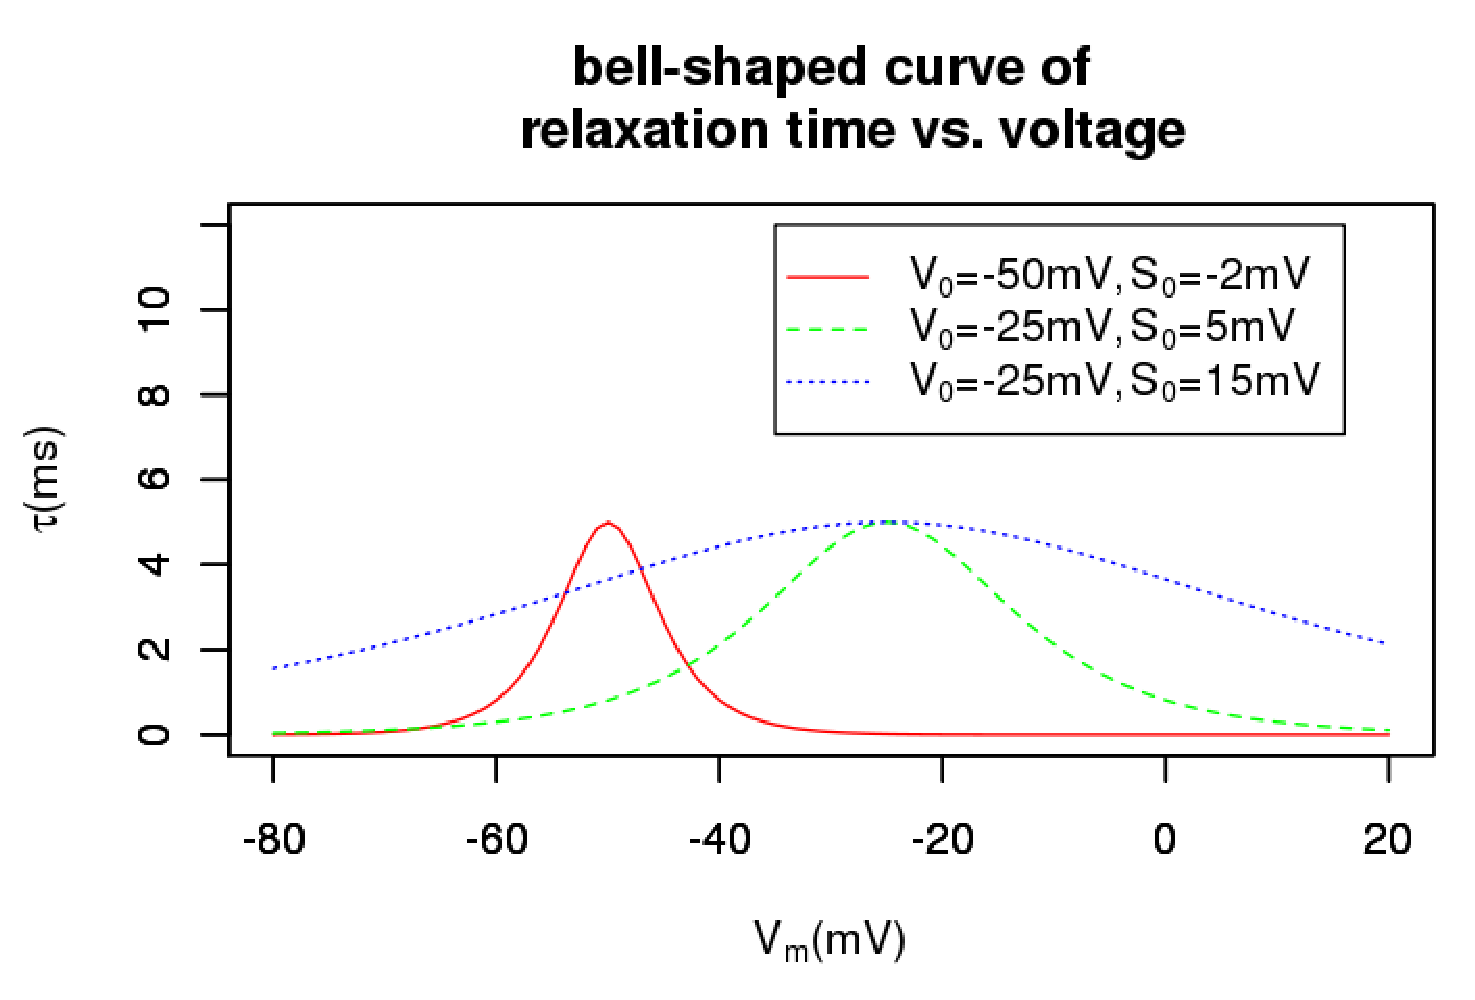
\includegraphics[height=6.5cm]{./images/chap2_tau_V.eps}}
  \caption{The characteristic relaxation time $\tau$ which are picked
    around the values of $V_0$ and have the width determined by $S_0$}\label{fig:tau_V}
\end{figure}

{\bf REMARK}:
\begin{itemize}

\item The curve of the mean open time $\tau(V_m)$ is a bell-shaped
  function of membrane voltage which is analogous to the well-known
  Hodgkin-Huxley mean open time constant for axonal excitation.

\item The higher the value of $\tau$, the longer the channels in open
  state.

\item The peak of the curve $\tau(V_m)$ are peaked around the values
  of $V_0$. $V_0$ is the membrane voltage at which the fraction of
  active ion channels is $f_\infty$.

\item The magnitude of $S_0$ determine the variance in the gating of
  channels, i.e. the larger $|S_0|$ the wider the width and the more
  channels to be in open state..
\end{itemize}

\section{Giant axon of the squid}
\label{sec:squid-giant-axon}

Squids squirt jets of water when they need to move quickly, as when escaping a
predator. To make this escape as fast as possible, they have an axon that can
reach 0.5 - 1.0 mm in diameter (signals propagate more quickly down large
axons). The squid giant axon was the first preparation that could be used to
do voltage clamp for measuring the kinetics of transmembrane current
(Sect.\ref{sec:transmembrane-current}).
%Squid axon is a nerve fiber with .5mm.


\begin{figure}[hbt]
  \centerline{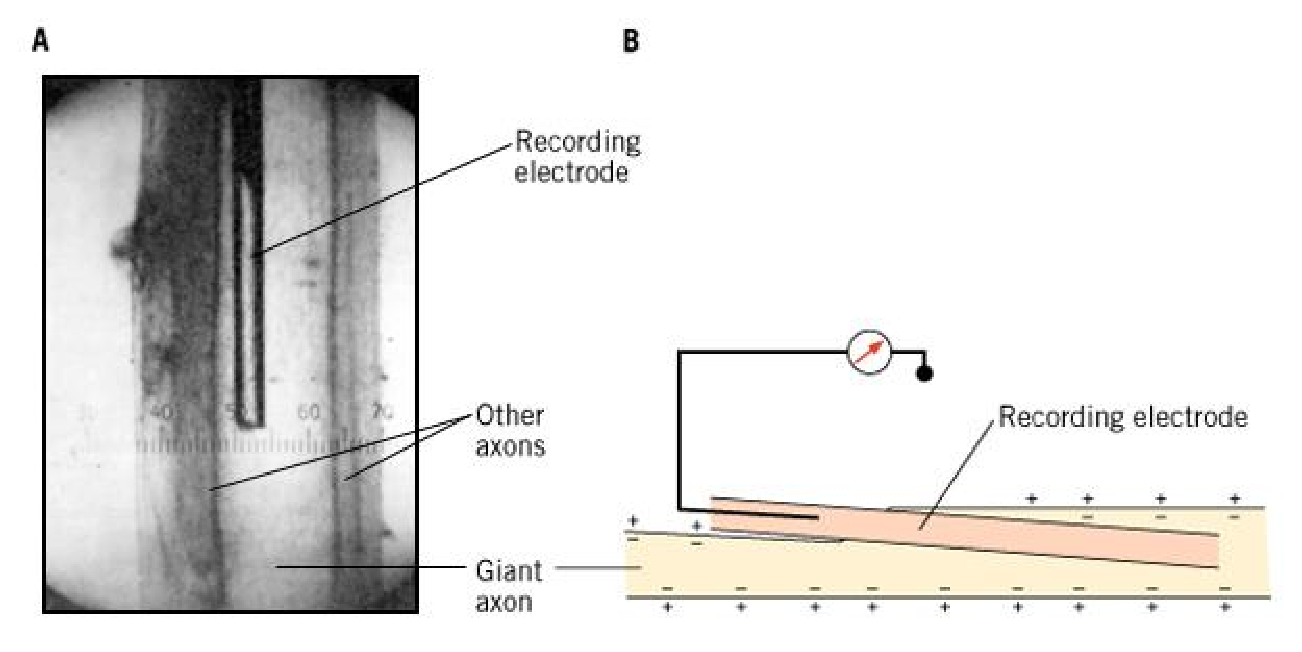
\includegraphics[height=5cm,
    angle=0]{./images/giant_axon.eps}}
  \caption{An experiment with squid giant axon}
  \label{fig:giant_axon}
\end{figure}

Early studies on physiological properties of ion channels utilized the squid
giant axons, as shown in Fig.~\ref{fig:giant_axon}. It was J.Z.Yong~ who first
discovered the applicability of squid axon to electrophysiological studies~\citep{young1936}.

Examples of concentration of different types of ions in squid giant axons and
mammalian neuron \citep{gilbert1990} at resting stage are shown in
Fig.~\ref{fig:ion_concentration}.  Due to the large amount of negatively charged
proteins in the cytosol, at resting state, intracellular charge $V_i$ is always
more negative than extracellular charge $V_o$.

\begin{figure}[htb]
  \centerline{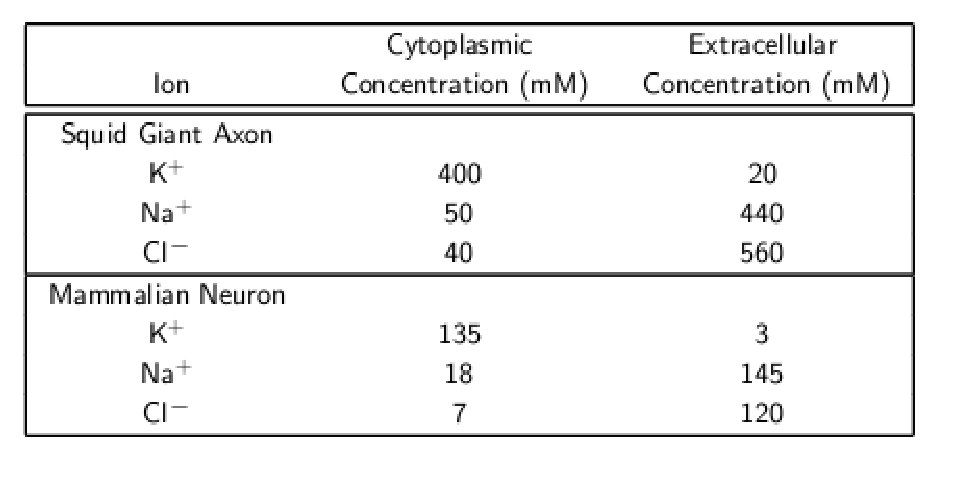
\includegraphics[height=5cm]{./images/ion_concentration.eps}}
  \caption{Ion concentration in squid giant axon and mammalian neuron
    at resting potential}\label{fig:ion_concentration}
\end{figure}

\textcolor{red}{In this chapter, mathematical models for reproducing
the AP in giant axon of the squid using Hodgkin-Huxley model is the major
topic}. In this model, the membrane potential is considered to be a function
of concentration of sodium, potassium and chlorine ions on either side of the
membrane, and by the relative permeabilities of the membrane to these ions.
In the last part of the chapter, we also discuss some models for AP in muscle
cells and Purkinje fibre that were based on Hodgkin-Huxley's model. This will
help creating the basis for the studying of the next chapters.

\begin{mdframed}

{\bf Knowledge base}: Negative ions are rarely permeated through
cell membranes. At the time the model was created, studies with isotopes shown
that the cell membrane permeates $\Na$, $\K$, $\Cl$, and water \citep{Leaf1959}.
The major role of \ce{Ca^2+} has not been confirmed. Thus, Hodgkin-Huxley model for
axons (to be studied in this chapter), only \ce{Na+}, \ce{K+},
\ce{Cl-} are examined. In muscle cells, \ce{Ca^2+} ions play
essential roles to (1) generate the prolonged AP (plateau phase) and
(2) {\it excitation-contraction coupling} (ECC), especially in
ventricular cardiac cells.

This form of elevation, first believed to be global
transient~\citep{fabiato1975cic}, yet later widely accepted by the hypothesis
of local elevation of calcium concentration, known as \ce{Ca^2+} {\it sparks}
(from RyR)~\citep{cheng1993cse} and \ce{Ca^2+} {\it puffs} (from
IP3)~\citep{parker1991rr}. In the scope of this chapter, we can ignore this.
\end{mdframed}

The ionic concentration between the cytoplasm and the extracellular
milieu are not the same. Indeed, it is the gradient that help cells
maintaining the normal functional role,
Fig.~\ref{fig:ion_concentration}.



\textcolor{red}{In this chapter, we will study the dynamics of a
single ion channels in a more detailed and more realistic manner,
focusing on 3 transmembrane ionic channels (\ce{Na+}, \ce{K+},
\ce{Cl-}) in squid axon used by the classic Hodgkin-Huxley
model. Other types of ionic channels (LCC, IP3, RyR...), for other
types of cells, will be discussed in other chapters}
(Chap.~\ref{chap:dhpr-models}, Chap.~\ref{chap:models-pumps},
Chap.~\ref{chap:ip3r-models}, Chap.~\ref{chap:ryr-models}).




\section{Q10 factor}
\label{sec:q10-factor}


Not all experiments are carried out at the same temperature. In this section, we
will learn how to map the result from one temperature to another one.
As mentioned in the previous chapter, the temperature T affect the kinetics of a
chemical reaction. In gating channels, this is also correct.
This dependency is expressed in the quantity $\Phi$ that change of every
10$^\circ$C.
\begin{equation*}
  \begin{split}
    dm/dt &= \Phi[-\frac{m-m_\infty(v)}{\tau_m(v)}]\\
    dn/dt &= \Phi[-\frac{n-n_\infty(v)}{\tau_n(v)}]\\
    dh/dt &= \Phi[-\frac{h-h_\infty(v)}{\tau_h(v)}]\\
  \end{split}
\end{equation*}
NOTE: another way to interpret is the change in the time constants
\begin{equation}
\tau_\text{newTemperature} = \frac{\tau_\text{oldTemperature}}{\Phi}
\end{equation}

\begin{framed}
  Q10 is a unitless
  quantity\footnote{\url{http://www.csupomona.edu/~seskandari/physiology/physiological_calculators/Q10.html}}
  that tells the increase in reaction rate for every 10-degree rise in
  temperature. Suppose $R_i$ is the rate at temperature $T_i$, then
  \begin{eqnarray*}
    Q10 = \left(\frac{R_2}{R_1}\right)^{\frac{10}{T_2-T_1}}
  \end{eqnarray*}
  If the reaction is completely temperature-independent, then
  $Q10=1.0$. NOTE: $Q10 \approx 1$ for the diffusion of ions and
  molecules in bulk solution. For many biological processes, especially
  those involving large-scale protein conformational change, $Q10 > 2$.
\end{framed}

% and
% \begin{enumerate}
%   \item
% \end{enumerate}

$\Phi$ is the coefficient (Tadj: or temperature adjustment)
that tells the change of the three conductance variables following the
change in temperature
\begin{eqnarray*}
  \Phi=(Q10)^{(T_C-6.3)/10}
\end{eqnarray*}
All formulation obtained in HH model to be discussed later are measured at
$T_C=6.3$ ($^\circ$C), with a $Q10=2.3$, thus $\Phi=1$. In the case data is
collected from the condition of different temperatures, we need to adjust them
accordingly to the same temperature.

\begin{mdframed}

  {\bf Knowledge base}: Ion currents change at different temperature and it may
  greatly affect the action potential. Q10 is a unitless
  quantity
  \footnote{\url{http://www.csupomona.edu/~seskandari/physiology/physiological_calculators/Q10.html}}
  that tells the increase in reaction rate for every 10-degree rise in
  temperature. Suppose $R_i$ is the rate at temperature $T_i$, then

  \begin{eqnarray*}
    Q10 = \left( \frac{R_2}{R_1} \right)^{\frac{10}{T_2-T_1}}
  \end{eqnarray*}

  If the reaction is completely temperature-independent, then
  Q10$=1.0$. NOTE: Q10 $\approx 1$ for the diffusion of ions and
  molecules in bulk solution.

  For many biological processes, especially those involving large-scale protein
  conformational change, Q10$ > 2$.

\end{mdframed}

\section{Tonic conductance vs. Phasic conductance}
\label{sec:tonic-conductance}
\label{sec:phasic-conductance}

The conductance, measured in skin is traditionaly characterized by
 two types - tonic and phasic - which can roughly be thought of as "the smooth
underlying slowly-changing levels" vs. "the rapidly changing peaks."

{\bf Tonic conductance}: the change in conductance is a slowly changing in
level, which explains the conductance in the absence of any particular discrete
environmental event or external stimuli, Fig.\ref{fig:rhythmic_contraction_SMC}.
Tonic changes in the skin conductance level typically occur in a period of from
tens of seconds to minutes.

{\bf Phasic conductance}: the change in conductance is typically associated with
short-term events, i.e. with abrupt change (or showing 'peak') in the
conductance level.
It is typically the recorded value in the presence of discrete environmental
stimuli (sight, sound, smell, cognitive processes that precede an event such as
anticipation, decision making, etc).


\section{K channels}

The universally appearance of K channels make them not possessing a
single kinetics. Indeed, there are more than one type of K channels
(Chap.\ref{chap:K_model} and one chapter in the ThermoStat-BioPhysics book):
Later researches had revealed a third conductance, known as
$g_A$. Both $g_K$ and $g_A$ are inward and are carried by Potassium
ion. However, $g_A$ activate at the subthreshold potential
range\footnote{subthreshold = small-signal, here it is below -40 mV}
and has the time constant between that of $g_{Na}$ and
$g_K$\citep{connor1971prf}. These current account for the repetitive
firing of spikes.  The question is
\textcolor{red}{how $K_A$ channel help a cell fire repetitively at low
  frequencies?}. The answer lies in the events of interspike interval.
\begin{itemize}
\item At the end of the first AP, $K_A$ channel are all inactivated,
  but K channels are so strongly activated that the cell
  hyperpolarized despite the steady applied stimulus current.
\item This hyperpolarization gradually remove inactivation of $K_A$
  channels, and also shut down K channels. This allow the cell
  membrane to depolarize again.
\item This small depolarization allow $K_A$ channels to open again,
  and the outward current $I_A$ can counterbalance the inward stimulus
  current $I_\app$.
\end{itemize}

$g_A$ is predominant between the interspike interval, and mainly to
counterbalance the inward current $g_{Na}$ and the stimulus current. The
new equation is
\begin{equation}
  \label{eq:546}
    % I_{m} = \Csc\frac{dV_m}{dt} + I_{\ce{Na}} + I_{\ce{K}} + I_{leak} - I_\app
      \Csc\frac{dV}{dt} = -g_{\ce{Ca}} (V-V_{\ce{Ca}}) - g_{\ce{K}}  (V -
  V_{\ce{K}}) - g_{\ce{A}}(V-V_{\ce{A}}) - g_L (V - V_L) + I_\app
\end{equation}

In later chapters, $I_K$ is called the delay-rectifier $I_\Kdr$;
while $I_{K,A}$ is from the low AHP Ca-activated current
$I_{K-AHP}$. In many cases, it's very difficult to distinguish
$I_{K,A}$ from $I_\Kdr$.

% {\bf NOTATION}: There are two sets of subscript, the first one to
% denote the process (B and
% A)\footnote{analogous to activation $m$ and inactivation $h$ in HH
%   model}, and the second one to denote the channel type (I, K, A).
%
%
% The capacitance is the ratio of the applied current vs. the rate of
% change of the initial voltage.
% \begin{eqnarray}
%   \label{eq:547}
%   I_\app = \Csc\frac{dV}{dt}
% \end{eqnarray}
% In the vicinity of $-40$ mV, A channels are completely inactivated,
% while I and K channels haven't been appreciably activated. Thus, the
% conductance at this condition is assigned to $g_L$ (leak
% conductance), which is the slope of the I-V curve, and the voltage at
% this point is the leakage equilibrium potential $V_L$.
%
% $g_{Na}$ give rises after a delay to a peak and then decrease
% exponentially. Thus, $g_{Na}$ is defined using the same form as one in
% HH model.



\chapter{Experimental recordings}

Long before the discovery of ion channels, it has been known that there is a
voltage gradient between the inside and outside of the biomembrane of many
cells, as recorded using electrodes - one injected into the cell's inner medium
and one put into the extracellular medium (Sect.\ref{sec:electrode}).
This happens because the biomembrane is organized in such a way that behave like
an electric circuit (Sect.\ref{sec:electrical-property-biomembrane}).

The capability of recording electrical activity of a single cell,
Fig.\ref{fig:recording-Vm}, date back to the mid twentith centity with two
events (1949-1952) that profoundly affected the field of electrophisiology was
(1) the introduction of intracellular glass microelectrode
(Sect.\ref{sec:micro-electrodes}) by Gilbert Ling and Ralph Gerard, (2)
development of ionic theory of action potential (AP) by Katz, Hodgkin and Huxley
\citep{graham1946, cole1949, hodgkin1952ap} that explains the dynamics of
membrane resistance.

\section{Cell preparation techniques}

\begin{figure}[hbt]
  \centerline{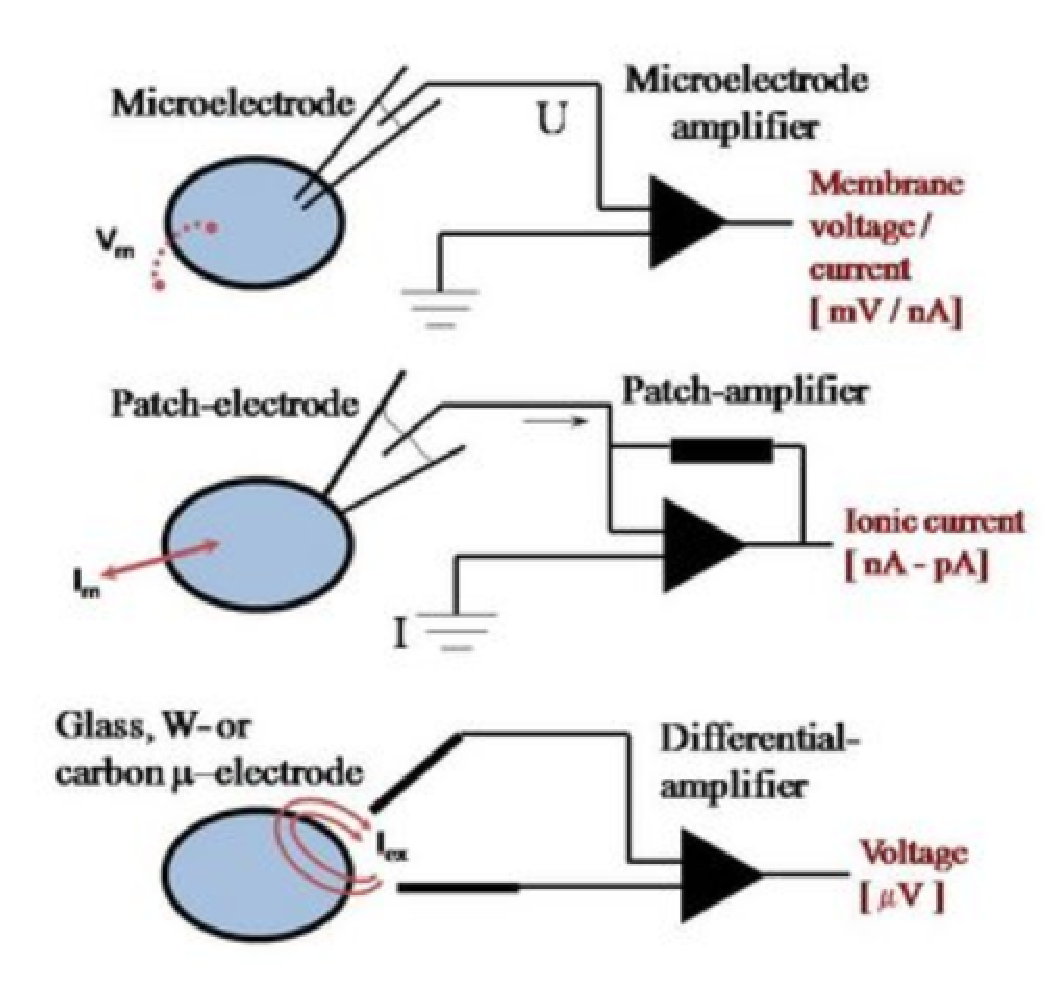
\includegraphics[height=4cm,
    angle=0]{./images/Cell-recording-techniques.eps}}
\caption{Schematic diagram of different cell recording techniques: (A)
microelectrode; (B) Patch-electrode; (C) Extracellular recording}
\label{fig:Cell-recording-techniques}
%http://mhs3.mp.kanazawa-u.ac.jp/eng/staff/rihabiri/shosaku.html
\end{figure}

Fig.\ref{fig:Cell-recording-techniques}:
\begin{enumerate}

  \item {\bf extracellular recording}
  (Sect.\ref{chap:extracellular-recording}):  if multiple cell recordings are
  desired, they probably are a necessity.
  \textcolor{red}{Measure voltage changes which is often small amount ($\mu$V)}.


  \item {\bf intracellular recording}: record the potential difference between
  the intracellular space (at the point of insertion) and some extracellular
  reference point. \textcolor{red}{Measure voltage different and current
  (mV, nA)} - Sect.\ref{sec:intracellular-recording}

  \item {\bf patch-clamp recording} (including whole-cell patch-clamp): can
  records current via a few channels or many channels.
  \textcolor{red}{Measure ionic currents only; yet for a wide range (pA - nA)}
  - Sect.\ref{sec:patch-clamp}

  The pipette is bigger, and forms a tight (i.e. suction) with the outer-side of
  the cellular membrane, i.e. not breaking the cell membrane, and measure the
  current pass-through the membrane when the ion channels/receptors on the
  membrane patch covered by the pipette opens.

\end{enumerate}
\url{http://www.scholarpedia.org/article/Intracellular_recording}

\begin{figure}[hbt]
  \centerline{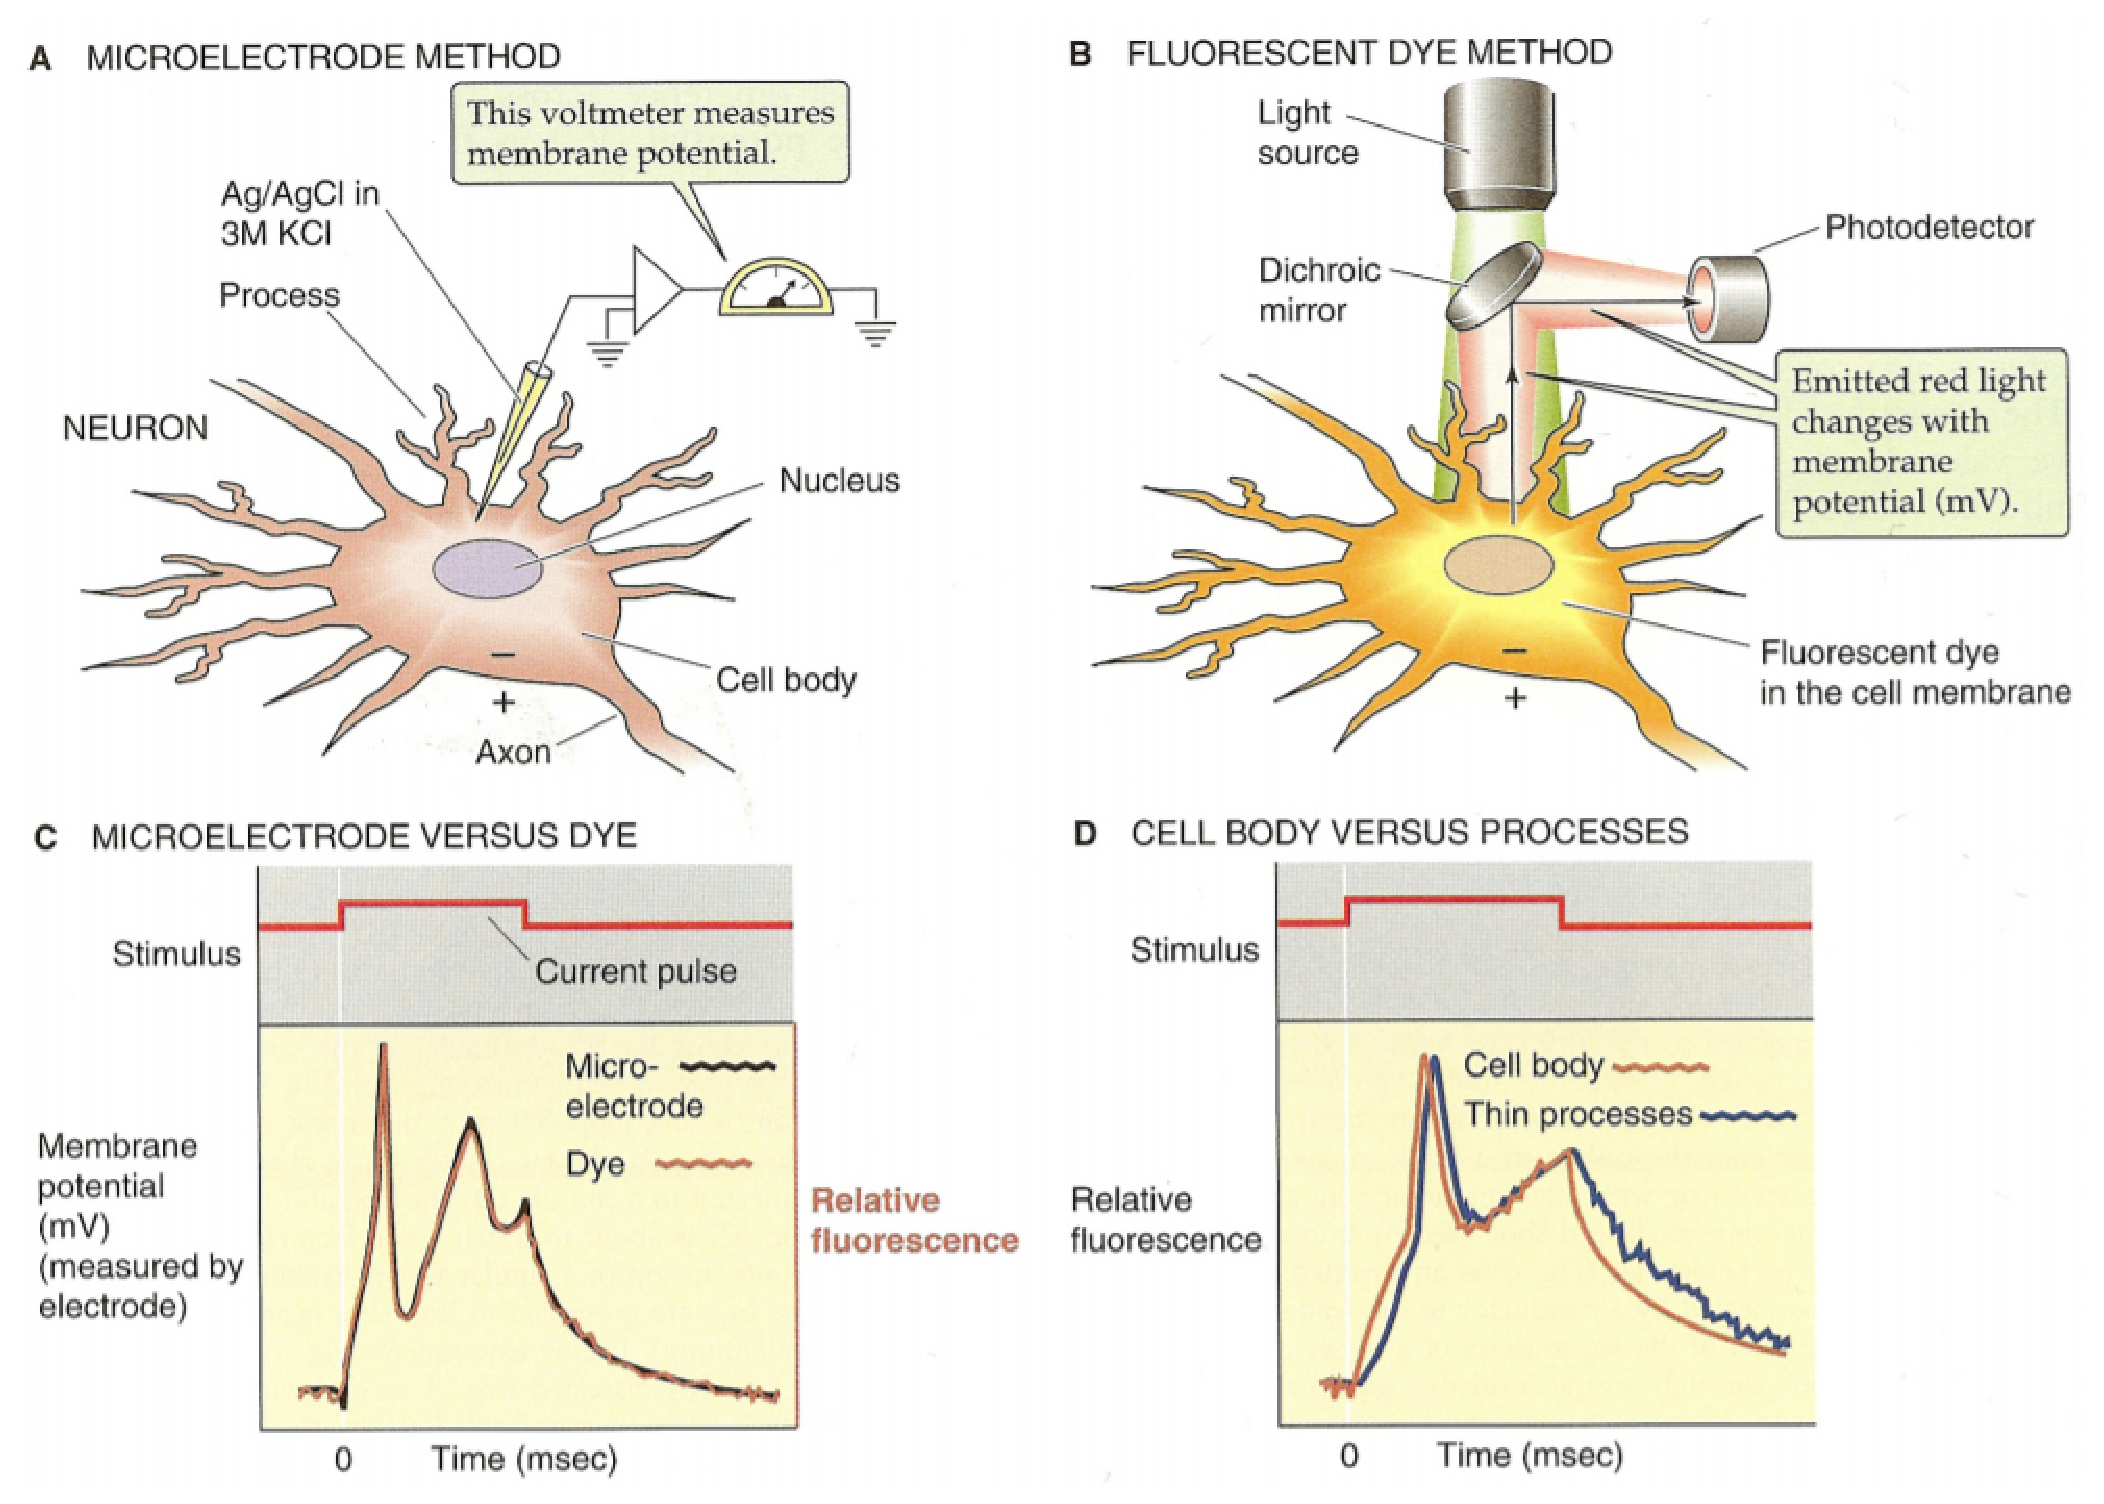
\includegraphics[height=4cm,
    angle=0]{./images/recording-Vm.eps}}
\caption{Two different techniques for recording Vm: (A) electrode, (B)
fluorescent dye. Compare results: (C) method (A)  and (B) at same location; (D)
same recording technique of Vm at different location in the same cell}
\label{fig:recording-Vm}
\end{figure}

\subsection{Cell dissociation techniques}
\label{sec:technique-cell-dissociation}

\subsection{-- from brain}

Reference videos:
\begin{itemize}
  \item isolate the hippocampus:
  \url{https://www.youtube.com/watch?v=tdEvicXkMCk}

  \url{https://www.youtube.com/watch?v=Upf15CB29V4}

NOTE: The CA1 region of the hippocampus was used predominantly in developing and
testing the method of cell isolation as it is a region rich in cells of a
stereotyped morphology.

  \item
\end{itemize}

\textcolor{red}{There are different ways to dissociate mouse brain tissue}, as
the effectiveness of each method depends upon {\bf IMPORTANT FACTORS}:
like age of mice (embryo, young or adult) region of the brain you use (e.g.
cerebellum, cortex, etc.) and protocol you use.


\begin{itemize}
\label{sec:enzymatic-treatment-technique-dissociate-cells}

  \item enzymatically approaches: trypsin, papain, etc.

It has been shown that papain treatment provided better survival of hippocampal
neurons (PMID: 9128149).

NOTE: Enzymatic digestion alone is ineffective, it is necessary to agitate the
slices to achieve dissociation. Low temperatures (< 15$^\circ$C) after enzymatic
digestion, reduced the yield of cells to zero.

  \item non-enzymatically approaches: like mechanical dissociation, or Versene
  (that is EDTA -based solution)
\end{itemize}
but overall the most important things for successful achieving of your goals is
time and temperature (bearing in mind hypoxia and inflammation of brain tissue)
and trituration, which should be done fast but gentle - fire polished Pasteur
pippets of different diameters for trituration should be employed (and try to
avoid bubbles during trituration)



Pioneers with their own protocols:
\begin{itemize}

  \item  (Numann and Wong, 1984) isolating neurons based on papain digestion,
  e.g.  Papain Dissociation Kit from Worthington (since it has been tested for
  use on brain tissue).

Neither collagenase nor hyaluronidase alone or in combination with trypsin
proved effective.

Papain is recommended for brain tissue digestion (particularly
embryonic/postnatal).  Papain yielded cells with clean surfaces but they did not
prove as viable as those subjected to trypsin digestion. A better protocol is
introduced by Huettner, Baughman (1986).


  \item Huettner \& Baughman (J Neurosci. 1986 Oct;6(10):3044-60.  Primary
  culture of identified neurons from the visual cortex of postnatal rats.
  Huettner JE, Baughman RW.):

\textcolor{red}{This is the recommended protocol using papain} since it helps
preserve the viability of neurons derived from postnatal animals.

  \item  R. K. S. Wong and A. Kay (1986) introduced technique to isolate neurons
free of cellular debris and glial investment, and then a Giga-Ohm seal (in the
range 5-100 G$\Omega$) is formed for patch-clamping
(Sect.\ref{sec:patch-clamp}). This is better the the above method in both yield and quality.

\textcolor{red}{how to make cell separation easier}? A PIPES-based saline
consistently yielded more cells than an equivalent HEPES-buffered saline. It was
not sure how PIPES-based saline is better; but the nature of the salines that
facilitate dissociation are suggestive of the involvement of intracellular pH. A
low extracellular pH and an elevated CO2 level, should lead to a decline of
intracellular pH, while the absence of extracellular bicarbonate ions might
disrupt intracellular pH regulation, if a bicarbonate-dependent acid extruding
mechanism is a necessary part of pH regulation (Roos and Boron, 1981).
It was speculate that a lowered intracellular pH could disrupt cell-cell
interaction, by affecting the extracellular glycoproteins that mediate this
nexus or by causing glia to retract, perhaps triggered by the closure of gap
junctions, caused by the fall in pH (Connors et al., 1984).

{\bf Bicarbonate-buffered saline} (in mM):  NaCl 114, KCl 5,  $\ce{CaCl_2}$  1,
$\ce{MgCl_2}$ 1, $\ce{NaHCO_3}$  26, D-glucose 25, HEPES 10 at pH 7.4.

Two sorts of solution were found to promote dissociation of brain slices; either
a bicarbonate-buffered saline with a  pH between 6.2 and 6.5 under a  5\%
CO2/95\% 02 atmosphere, or a  PIPES-buffered saline under a  100\% 02 atmosphere
at pH 6.2-7.4. This gives cell of 10 fold greater than that obtained with a
bicarbonate-buffered saline.


\textcolor{red}{Solutions}: these solutions (in mM) are used during the course
of dissociation procedure
\begin{itemize}
  \item PIPES saline: NaCl 120, KCl 5, $\ce{CaC1_2}$ 1, $\ce{MgCl_2}$ 1,
  D-glucose 25, PIPES 20 (piperazine-N, N'-bis [2-ethanesulfonic acid]) (pH 7.0).

WHEN TO USE: The brain is rapidly but carefully removed and placed in cold
(about 5$^\circ$C) PIPES saline that has been bubbled with 100\% 02.

NOTE: The brain region of interest is blocked-off using a scalpel blade; and
slices of about 650 $\mum$ thickness is cut out using Mcilwain tissue chopper
device \footnote{\url{https://www.youtube.com/watch?v=Li4SoZaleBE}}.
The slice is put on central chamber (at 32$^\circ$C) with 100\% 02 introduced
continuously (flow rate about 150 ml/min) into the chamber.
\textcolor{red}{Slices can be held in the chamber up to 10 h after commencing
the enzymatic digestion while cells are still usable}.

   \item DMEM: Dulbecco's modified Eagle's medium with HEPES 25, D-glucose 25
(supplied in this modified form by Gibco, Grand Island, N.Y.).

WHEN TO USE: When cells are needed, two slices are removed from the chamber and
placed in approximately 1 ml of DMEM, held in a small glass
\textcolor{red}{Neurons should be prepared just before recording, as isolated
cells last for not more than 2 hours}.

DMEM greatly improves the yield and viability of cells only when used at the
trituration stage.

   \item HEPES saline: NaCl 140, KCl 5, $\ce{CaCl_2}$ 1, $\ce{MgCl_2}$ 1,
   D-glucose 24, HEPES 10 (pH 7.4).

WHEN TO USE: The neurons are allowed to settle on the bottom of the dish before
the DMEM is replaced with the HEPES saline, which is used during recording and
need not be oxygenated.

\end{itemize}

Also, it can hold cells in good condition, particularly with intracellular
solutions having fluoride as the predominant anion (see methods), for up to 1 h.
\textcolor{red}{The quality of the cell is heavily depending upon the skill of
operator}. The skill lies in the rapid removal of tissue with the minimum of
handling applied to the tissue and in a meticulous attention to detai.

\begin{mdframed}
Others have described methods for the bulk isolation of neurons from adult brain
(reviewed in Althaus and Neuhoff 1982, and Schaffner and Schnaar, 1983).
Most of these methods are complex, time consuming and often  do not yield cells
that are free of glial investments.
Such methods have been aimed at   the preparation of large quantities of cells
for biochemical experiments.
\end{mdframed}

  \item {\bf in vitro} conditions: you should consider replacing part (1/3) of
  the growth media after 48-72 hours after you've plated your cells (in vitro
  conditions),  in order to remove all the dead cells, cell debris and
  inflamatory or appoptotic factors released by dying cells in your culture
  dish.


\end{itemize}
\url{https://www.researchgate.net/post/What_is_the_best_way_to_enzymatically_dissociate_mouse_brain_tissue_that_gives_a_high_yield_for_all_cell_types_neurons_astrocytes_microglia}

% KAY, A. R. AND WONG, R. K. S. Isolation of neurons suitable for patch-clamping
% from adult mammalian central nervous systems. J. Neurosci.
% Methods 16: 227-238, 1986.


Works: Huguenard, Hamill, Prince (1988)

\subsection{-- from cultured neurons}

Acutely isolated cells with cultured neurons:

\subsection{in vitro recordings}


\subsection{in vivo recordings}

\section{Physiological recording in excitable cells (neurons, myocytes)}

Data acquisition (DAQ) is the process of measuring an electrical or physical
phenomenon such as voltage, current, temperature, pressure, or sound with a computer.
A DAQ system consists of 
\begin{enumerate}
  \item  sensors, 
  
  \item DAQ measurement hardware, and 
  
  \item a computer with programmable software.
  
  LabView (Sect.\ref{sec:LabView}) from National Instruments.
  
\end{enumerate}
\url{http://www.ni.com/data-acquisition/what-is/}

%The communication between neurons in real time (from $\mus$ to hours) can be
%detected using
\begin{itemize}
  \item {\bf Current-clamp } (Sect.\ref{sec:current-clamp-protocol}): to measure
  voltage

  \item {\bf Voltage-clamp } (Sect.\ref{sec:voltage-clamp-protocol}): to
  estimate membrane conductance (via measuring membrane currents)

\end{itemize}

Review: \citep{cummins2009, perkins2006}.
\url{http://www.utdallas.edu/~tres/microelectrode/microelectrodes_ch04.pdf}

\url{http://www.utdallas.edu/~tres/microelectrode/microelectrodes_ch10.pdf}

\subsection{LabView}
\label{sec:LabView}

LabView has seamless hardware integration, approachable programming, and
built-in analysis algorithms, LabVIEW reduces the complexity of automation and
customization.

\subsection{WinFluor}
\label{sec:WinFluor}

\url{https://github.com/johndempster/WinFluorXE}

\url{https://github.com/johndempster/WinFluor}

NI-DAQmx and Traditional NI-DAQ are two independent drivers, each with their own
unique DLL's and functions.

Error:
\begin{verbatim}
Application has failed to start because nidaq32.dll was not found
\end{verbatim}
\url{http://digital.ni.com/public.nsf/allkb/F7F09E0377369C7586257150005D00F3}


 


\subsection{pClamp (Axon Systems)}
\label{sec:pCLAMP}

pCLAMP applications for controlling and analyzing electrophysiological
experiments with computers
\begin{enumerate}
  \item DOS-compatible version 1.0 (1973) in Caltech: originally used for
  kinetic studies on nicotinic acetylcholine receptors and on voltage-sensitive currents

  \item converted to PC-compatible software in mid-1982 and have been in use
  since 1983

  \item in 1984, licensed to Axon Instruments, Inc.

  \item in 1998: first Windows version, pCLAMP 7

  \item in 2002: first full conversion from DOS to Windows.

support for a variety of synaptic data (long-term potentiation/depression
[LTP/LTD] and minis), as well as action potentials.

  \item in 2006: pCLAMP 10 was released and also Molecular Devices Corp acquired
  Axon Instruments, Inc

  %\item
\end{enumerate}

\subsection{-- ABF file format}
\label{sec:ABF-file-format}

The Axon Binary File format (ABF) was created for the storage of binary experimental data.
It originated with the pCLAMP suite of data acquisition and analysis programs, but is also
supported by AxoScope Software. 
\begin{itemize}
  \item version 1.x
  
  \item version 2.x: released with pCLAMP 10 in 2006
  
  MAJOR CHANGES: the file header is now of variable length
\end{itemize}

The file forma is proprietary, but readers can be created by third-party
developers by using the ABFFIO library.
\begin{itemize}
  \item Matlab: 
  
abf 1.x: \url{https://www.mathworks.com/matlabcentral/fileexchange/6190-abfload}

abf 2.x: 

  \item 
\end{itemize}


\subsection{-- Components}

\begin{itemize}
  
  \item  Clampex (data acquisition) - patch-clamp data (with generate stimulus
  in different waveforms); and measure any physical parameter that can be
  linearly converted to a voltage (e.g. end-plate current, fluorescent signals,
  pressure)

Clampex 10.2 save files in ABF 2.x format.

  \item Clampfit (data analysis): parameter fitting - Sect.\ref{sec:Clampfit}

  \item AxoScope (background chart editing) - a subset of Clampex (but no
  episodic stimulation mode)

  \item MiniDigi (two-channel digitizer)

\end{itemize}

\section{Estimate current passing through a given channel type or a single
channel}
\label{sec:transmembrane-current}

The current passing through a given channel type is estimated via the
transmembrane current by blocking all other channel types, using proper blockers
or antagonists. Two broad types
\begin{enumerate}
  \item voltage-gated ion channels - Sect.\ref{sec:data-acquisition}

  \item ligand-gated ion channels -
  Sect.\ref{sec:measure-current-Ligand-activated-channels}
\end{enumerate}

Remember the total transmembrane current density $I_m$ is divided into
(1) capacitive current, (2) leak current, and (3) ionic currents which are in
parallel. The one we measure is the combination of 3 components; but the one we
are interested is the third component. So subtraction of capacitive current
(Sect.\ref{sec:capacitive-current-subtraction}) and leak current
(Sect.\ref{sec:leak-current-subtraction}) are needed.

The electric circuit established to measure the transmembrane current
$I_m$ (pA) which can be mapped to current density (pA/$\cm^2$) by estimating
the surface area $A$ (cm$^2$).
\begin{equation}
I_m = \Csc \frac{d\Vm}{dt} + \sum_{i=ion} I_{i} + I_\leak
\end{equation}
with current units (pA/cm$^2$).


% \section{Techniques to record data from voltage-gated vs. ligand-gated ion
% channels}

 
\section{-- Voltage-dependent ion channels}
\label{sec:data-acquisition}
\label{sec:measure-current-Voltage-activated-channels}

Suppose the gating of an ion channel is mainly/purely voltage-dependent, the
current we estimate is the transmembrane current $I_m$ which can be detected
using voltage-clamp protocols (Sect.\ref{sec:voltage-clamp-protocol}.
% electrophysiological techniques, such as voltage-clamp, allow us to measure the
% voltage (at the membrane surface) or current (at a particular voltage-gated ion
% channel) over time.

\begin{itemize}
  \item the earliest experiment in electrophysiology started with Jan Swammerdam
  (1637-1680) who did early experiment to study muscle contraction and
  neurophysiology using frog leg.

  \item Luigi Galvani (1737-1798) showed the first experimental evidence of
  electrical activity by using metal wires in frog muscle and triggering leg
  twitched.

  \item Cole and Marmont (1947) developed voltage-clamp technique
  for whole-cell recording (Sect.\ref{sec:voltage-clamp-Cole-Marmont}).

  \item Hodgkin and Huxley did the first intracellular measurement of AP in
  squid giant axon (Sect.\ref{sec:voltage-clamp-hodgkin-huxley})

  \item Graham impaled micro-pipettes into skeletal muscle fibers

  \item Bert Sakmann and Erwin Neher developed patch-clamp technique
  (Sect.\ref{sec:patch-clamp}) which is a refinement of voltage-clamp technique
  for single-channel recording
\end{itemize}


Depending upon the voltage-clamp protocol
\begin{enumerate}
  \item whole-cell clamp (Chap.\ref{chap:voltage-clamp-whole-cell}): current
  passing through a single type of ion channel

  \item patch-clamp (Chap.\ref{chap:voltage-clamp-patch}):  current passing
  through one or a few ion channels of a given type.
\end{enumerate}
it can be used to derive the kinetics of ensembled behavior or of single
channels. Under the voltage clamp protocol, the voltage is forced to change in
a square step fashion, as rapidly as possible, from a holding value to a
conditioning step value. This is induced by an injected current $I_\app$ (pA)
which keep adjusted.
\begin{itemize}
  \item upon the short time step ($\Delta t$) that $\Vm$ change from one value
  to another: this generate a capacitive current $I_c$ -
  Sect.\ref{sec:capacitive-current}, so we would see a brief spike of this
  capacitive current

  \item once the voltage reaches the new value, $d\Vm/dt=0$ so capacitive
  current is zero; thus, the transmembrane current now comprises only the ionic
  current

\end{itemize}

In a voltage-clamp procotol, we also applied an injected current $I_\text{app}$
(pA)
\begin{equation}
I_m = \Csc \frac{d\Vm}{dt} + I_\leak + \sum_{i=ion} I_{i} + \frac{1}{A}
I_{\text{app}}
\end{equation}
with 'estimated surface area' A (cm$^2$).


In a cable, with propagated membrane potential (Sect.\ref{sec:cable-axon}), if
there is a gradient in membrane potential; the transmembrane current
of the compartment $j$-th, is the difference between current passing through it
from two adjacent compartments (based on Kirchoff's law)
\begin{equation}
I_{m;j} = I_{j-1,j} - I_{j,j+1}
\end{equation}

References:
\begin{itemize}
\item \url{http://www.nature.com/nature/focus/ionchannel/#archive}
\item \url{http://www2.montana.edu/cftr/IonChannelPrimers/beginners.htm}
\item \url{http://www.sophion.dk/Technology/ion_channels}
\item \url{http://www.whatislife.com/reader/channels/channels.html}
\item \url{http://www.cnsforum.com/imagebank/item/rcpt_sys_nic_ag1/default.aspx}
\item \url{http://www.biologyreference.com/Ho-La/Ion-Channels.html}
\item
  \url{http://www2.montana.edu/cftr/IonChannelPrimers/ion_channel_history2.htm} (good)
\end{itemize}

\subsection{Leak and capacitive current subtraction}
\label{sec:P/N-subtraction}
\label{sec:current-subtraction}

In voltage-gated channels, the voltage impulse can induce a passive current by
redistributing the charges in membrane capacitance
(Sect.\ref{sec:capacitive-current}) and has a characteristic exponential time
course. This current can easily exceed the single channel current by two orders
of magnitude.

To eliminate this current, P/N subtraction can be used, i.e. we create an
idealized passive response and subtract it
and automatic, yet it can increases the recording noise, and thus requires
(Sect.\ref{sec:capacitive-current-subtraction}). P/N subtraction is convenient,
additional recording time. The noise in the passive current can be removed by
fitting the passive current piecewise to appropriate functions (e.g.
exponential, ramp).

Note that subtraction of capacitive and leakage currents is purely cosmetic. It
does not actually improve the signal recorded. However, it may allow revealing
small current components that would otherwise be hard to identify.

Capacitative and leakage currents were subtracted digitally by the P-P/4
procedure (Bezanilla and Anlastrong 1977).

Correction for leakage can be made by fitting the traces to a flat or
sloping base line by linear regression analysis and then by redrawing the curves
relative to the fitted base line.

\subsection{-- Capacitive current substraction}
\label{sec:capacitive-current-subtraction}

At transient of voltage in voltage-clamp
(Sect.\ref{sec:voltage-clamp-current-components}), the change in charge
separation leads to the capacitive current, once the new potential is reached,
there is no capacitive current. When there is a change in potential, \ce{Na+}
open quickly and we see more \ce{Na+} go inside which cause an inward current.
However, the depolarization, beside activating sodium channel, also deactivate
them. Then, the \ce{K+} channels open and we see an outward of \ce{K+} current
while more \ce{Na+} have been closed.

How to remove the contribution of capacitance to the trace at the beginning?
Also, in practice, it is impossible to hold $\Vm$ fixed, but we can only keep
$\Vm$ vary in a small variation around $V_c$. However, this is enough to
generate the capactive current (Sect.\ref{sec:capacitive-current}). So, to
remove this 'background' current from the signal to give a better estimation of
ionic current, a process called {\bf leak substraction} is needed.

This leak substraction process can be done on-line or off-line.
There are 2 protocols, depending upon the experiment conditions.
Suppose the recorded current trace is given in
Fig.\ref{fig:capacitive-n-leak-subtraction}(A) which has both capacitive
current, leak current and ionic current
\begin{enumerate}

  \item if the recording is carried out in both conditions (with and without
  blockers), the subtraction of the two signals (traces) immediately remove the
  capacitive current from the ionic signal as the capacitive signal is
  independent of the channel blocker agents.

  \item (if the above is not possible) P/N subtraction - first proposed by
  Bezanilla and Armstrong (1977) can be used:
  \begin{itemize}

    \item first measure the trace contributed only by capacitive
     current using a series of N (typically N=4) voltage step of 1/N
    (i.e. 1/4 or -1/4 depending on polarity) amplitude of the test pulse from a
    potential at which no Vm-dependent channels are activated.

If N=-4, i.e. P/P-4 protocol, there are 4 hyperpolarizing pulses of (-1/4
amplitude, i.e. -145mv hyperpolarized with -25 mV step from -120mV holding
potential): these 4*(-1/4) amplitude trace is given in
Fig.\ref{fig:capacitive-n-leak-subtraction}(B).

%     \item then continue with 'test' voltage is
%     preceded by


\begin{figure}[hbt]
  \centerline{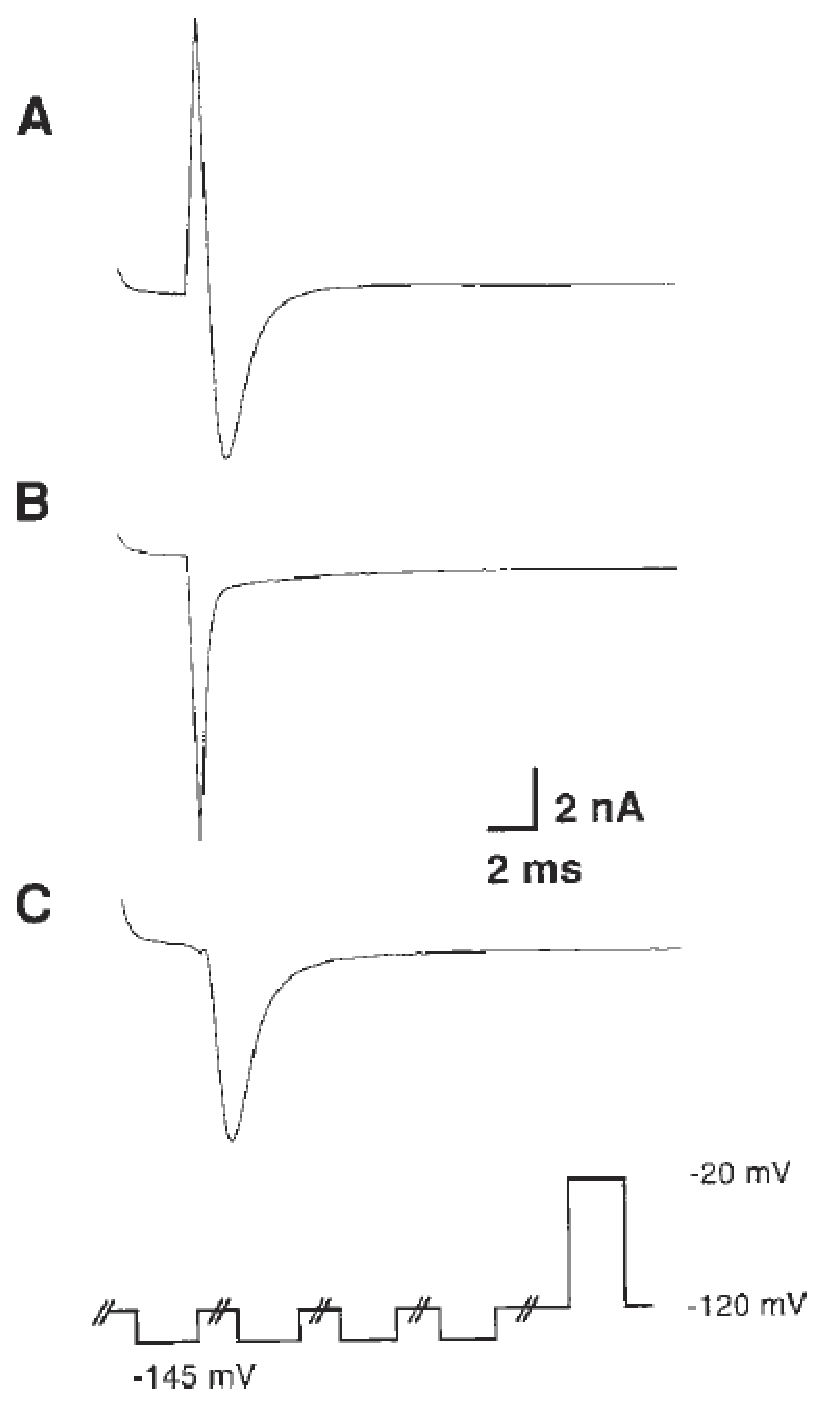
\includegraphics[height=6cm,
    angle=0]{./images/capacitive-n-leak-subtraction.eps}}
  \caption{(A) the trace recorded at voltage-clamp from -120 mV holding
  potential to -20 mV}
\label{fig:capacitive-n-leak-subtraction}
\end{figure}

    \item finally, subtracted (if N>0) or sum (if N<0) the signal of P/N
    protocol from/with the actual current trace of interest to give the trace of
    only ionic current, Fig.\ref{fig:capacitive-n-leak-subtraction}(C)

  \end{itemize}
\end{enumerate}

If capacitive currents are not of interest, it is recommended that P/4 leak
subtraction be performed on-line by the data-acquisition program because it
significantly reduces the amount of data stored.

\subsection{-- Leak substraction}
\label{sec:leak-current-subtraction}

It is important to obtain the 'leakage' current at potentials at which no
voltage-activated currents occur. Most often this can be achieved by stepping to
potentials negative to the resting potential, i.e. applying a hyperpolarizing
current.

However, some cells also express inwardly rectifying (or anomalous rectifying)
currents (Sect.\ref{sec:inward-rectifier-Kir}) that are active at the resting
potential and negative thereof. Under these circumstances leak currents must be
recorded at potentials (and/or condition) at which the I-V curve is linear and
no voltage-dependent currents are activated.

Once the trace is obtained, leak current (or $\Cl$ current) -
Sect.\ref{sec:leak-current}) is assumed to be a simple linear function of
voltage and the conductance $\bar{g}_\leak$ can be obtained by fitting that to
the function:
\begin{equation}
I_\leak = \bar{g}_\leak \times (\Vm - E_\leak)
\end{equation}

\subsection{Ramp generator: voltage ramp, current ramp}
\label{sec:voltage-ramp}

To perform voltage clamp or current clamp, we need a ramp generator.

In electronics and electrical engineering, a ramp generator is a function
generator that increases its output voltage up to a specific value, called a
ramp. So a small force is applied in increment to increase the voltage/current
to a new value via a series of motion, in stead of in one motion. Electrical
potential progression smoothed by the ramp generator, i.e.
to provide a nearly linear (current/voltage) ramp up/down.
\begin{itemize}
  \item A voltage ramp  is a voltage that is linearly increasing or decreasing
  at any rate.
\end{itemize}

Originally, ramp generators were implemented as analog hardware devices. Today,
this functionality is part of the software of a digital device.
\subsection{-- Step (voltage) clamp}
\label{sec:step-clamp}

In step clamp, the  steady state currents-vs-voltage is plot

\subsection{-- Ramp (voltage) clamp}
\label{sec:ramp-clamp}

The "ramp clamp" was so named to describe an experiment in which the control
voltage was swept with a linear increase in voltage with time (ramp) from a
resting level to a strong depolarized value.


The membrane current was plotted vs voltage directly and continuously.

The ramp clamp method generates current-voltage relations very much more rapidly than
using step clamps, and therefore seems ideal for a study of rapidly activating or time-
independent currents




\section{-- Ligand-activated ion channels}
\label{sec:measure-current-Ligand-activated-channels}

Ligand-activated ion channels, e.g. neurotransmitter-activated, currents are
perhaps easier to identify and isolate than their voltage-dependent counterparts
(Sect.\ref{sec:data-acquisition}).

The ionic currents are induced in a time-dependent manner based on the
application of exogenous ligands.
Ligand-gated current can be isolated from background noise by subtracting
recorded currents in the absence and presence of a given ligand.

\subsection{Fast-scan cyclic voltammetry (FSCV)}
\label{sec:FSCV}

Voltammetry studies the current as a function of applied potential, i.e. I=f(V).
The potential is varied arbitrarily either step by step or continuously, and the
actual current value is measured as the dependent variable.

Cyclic voltammetry - A voltammetric method that can be used to determine
diffusion coefficients.

Fast-scan cyclic voltammetry (FSCV) was developed by Julian Millar and
colleagues in London in the early 1980s.  FSCV in combination with carbon-fiber
microelectrodes became a very popular method for detection of neurotransmitters,
hormones and metabolites in biological systems, e.g. 5-HT, dopamine,
norepinephrine. \textcolor{red}{At 10 Hz (i.e. 100 ms temporal resolution)}, it
can samples the dynamic of neurotransmitter release and clearance.
\begin{enumerate}
  \item  The potential at the microelectrode is held at a potential insufficient to
oxidize dopamine (e.g., -0.4 V vs a Ag/AgCl reference electrode) and then
linearly ramped to an oxidizing potential (e.g., +1.3 V) and back at a high scan
rate (e.g., 400 V/s) multiple times each second.

  \item During positive sweep, dopamine at the surface of the electrode is
  oxidied to form {\it dopamine-o-quinone} (peak reaction at approximately +0.7
  V)

  \item During negative sweep, dopamine-o-quinone is
  reduced back to dopamine in the negative sweep (peak reaction at approximately
  -0.3 V).
\end{enumerate}
\url{http://www.jove.com/video/3464/presynaptic-dopamine-dynamics-striatal-brain-slices-with-fast-scan}

During the redox reactions electrons are transferred between these molecules and
the microelectrode (electrolysis).
This flux of electrons is measured (as current) and is directly proportional to
the number of molecules that undergo electro-oxidation.
 For quantification of changes in dopamine concentration over time, the current
at its peak oxidation potential can be plotted for subsequent voltammetric
scans. This approach can be utilized to make rapid chemical measurements in a
range of biological preparations and conditions.
\url{http://depts.washington.edu/pemplab/?page=fscv}

Fast-scan cyclic voltammetry offers real-time measurements of changes in
extracellular dopamine concentrations in vivo. With its subsecond time
resolution, micrometer-dimension spatial resolution, and chemical selectivity,
it is the most suitable technique currently available to measure transient
concentration changes of dopamine.



\subsection{Two-photon uncaging: neurotransmitter}
\label{sec:two-photon-uncaging}

To measure the role of neurotransmitter on receptors, it requires rapid and
localized application of neurotransmitters, e.g. glutamte.
Caged compounds are biological signaling molecules, e.g. caged glutamate,
inactivated by a photosensitive blocking group.
When these compounds absorb ultraviolet (UV) light, a covalent bond attaching
the caging group is broken, and an active signaling molecule is released.


To initiate the released of active neurotransmitter, light is used, i.e.
photon uncaging. However,  unfocused light can cause uncaging at above and below
the target cell which limits depth resolution.

A better technique is called {\bf two-photon uncaging}, i.e. a double-caged
glutamate that requires absorption of two photons for conversion to active
glutamate \citep{pettite1997}. Here, glutamate is caged by two groups whose
released required obsorption of two photons and thus limit the axial spread from
42um to only 17um, i.e. improve spatial resolution (Fig.3a in the paper).

This method was used to map the distribution of glutamate receptors on hippocampal pyramidal neurons
(Sect.\ref{sec:pyramidal-neurons}) to study AMPAR (Sect.\ref{sec:AMPAR}).

Assumptions:
\begin{enumerate}
  \item the light tapers to a leak 5.6 $\mum$ wide and $\approx$ 15 $\mum$ deep

  \item   any given depth z, the light forms a Gaussian spot with half-maximal
  radius rspot(z).

  Also, peak light intensity at the center of any cross-section must
  be versely proportional to the spot area $r^2_\spot(z)$. On that plane, at a
  point at lateral distance $r$ to the center, the light intensity
  is A(r,rspot(z)), with

  \item
\end{enumerate}

\subsection{ -- in vivo}

\citep{noguchi2011} developed a method to apply 2P uncaging of neurotransmitters in vivo of
neocortex of adult mice. They can measured in vivo at upto 200 $\mum$ from the
pial surface.

\section{Understand cell recording: measure voltage (current clamp), measure
current (voltage clamp)}
\label{sec:understand-cell-ephys-recording}

NOTE: Older patch-clamp amplifiers implement a different circuit that is less
suitable for voltage recording. However, to help understand the circuit
configuration easier, let's learn a simple circuit -
Sect.\ref{sec:current-clamp-protocol}.

{\bf The terminology used for describing the various resistances involved in
electrophysiological recordings is confusing.}
\begin{enumerate}
  \item {\bf series resistance} = {\bf access resistance} = {\bf electrode
  resistance} - Sect.\ref{sec:series-resistance}

  \item {\bf input resistance} (Sect.\ref{sec:input-resistance}) = the total
  resistance observed by the amplifiers which is equal to the sum of {\bf
  membrane resistance} and {\bf electrode resistance}.

NOTE: The former, i.e. membrane resistance, generally dominate the sum.

  \item Injection of a step current into a cell will generate a charging curve
  typically composed of one or more exponential components. The slowest is the
  membrane time constant, $\tau_m$
  (Sect.\ref{sec:membrane-time-constant}).
  Faster components may represent redistribution of charge within
  multicompartment cells.

\end{enumerate}


Kay, Wong (1986): on CA1 pyramidal neuron
\begin{enumerate}
  \item resting potential in the range -45 to -60 mV

  \item action potential: amplitude 80 to 110 mV

NOTE: the large overshoot can be attributed to the absence of sodium in the
intracellular recording solution that they used) -
Sect.\ref{sec:electrode-electrolyte-solution}.

  \item input resistance (Sect.\ref{sec:input-resistance}): 300 - 1000 Mega-Ohm
  (M$\Omega$) from

NOTE: The value is high compared to those obtained from slice preparation (with
50 - 120 M$\Omega$ at room temperature (Brown, Griffith (1983))). The
explaination could be the loss of distal dendritic membrane

\textcolor{red}{High input resistance} facilitates voltage-clamp analysis by
reducing the series resistance error (Sect.\ref{sec:series-resistance}).
Also, the abbreviated morphology minimizes space-clamp problems
(Sect.\ref{sec:space-clamp}).

  \item {\it test normal activity of the neuron}: isolated cells respond to the
  application of $\gamma$-aminobutyric acid (Numann and Wong, 1984) and
  glutamate (Kay et al., 1984), i.e. it respondes to GABAergic input and
  Glutamatergic input.

  \item out-side out configuration (Sect.\ref{sec:patch_clamp-outside-out}) can
  be used to record the current via a few channels on the patch.

  \item {\bf reduce the kinetics of current}: , e.g. varying extracellular
  concentration

Several procedures were used to reduce the magnitude of Na+ conductance in
mature neurons to ensure graded, voltage-dependent inward currents. These
included reduced extracellular $[\Na]_o$, submaximal tetrodotoxin concentrations
(i.e. reduce the number of opening $\Na$ channels), and reduced holding
potential (i.e. reduce the driving force).


\end{enumerate}

\section{Ringer's solution}
\label{sec:Ringer-solution}

In 1882, Ringer discovered the proper concentration of different ions in the
solution that keeps the isolated cardiac cells a normal functioning heart beat
for hours which allows further investigating of the cells {\it in vitro}. This
`saline' solution, known as {\bf Ringer's solution}, and later advances has
found the foundation for cellular physiology.

There are different variations in Ringer's solution to help understanding the
contribution of different ionic concentration to the behavior of the nerve
fibers (or excitable cells) - see (Adrian, Freygang (1962)).

\subsection{normal Ringer solution}

normal Ringer solution typically has
\begin{itemize}
  \item 2.5 mM $[\K]_e$

Osmotic coefficients (G) are from Robinson and Stokes (1959) and these have
been taken at a concentration of 100 raM. For Na2SO4 and K2SO4 the values are
extrapolated to 55 mM.
All solutions have equal osmotic pressures corresponding to a
concentration of 210 milliosmoles.

  \item
\end{itemize}

\subsection{$\Cl$-free and $\Na$-free Ringer solution: sucrose Ringer's
solution}
\label{sec:Ringer-solution-Cl-free-Na-free}

Here, sucrose replaces $\ce{NaCl}$.

\subsection{sulfate-sucrose Ringer's solution}
\label{sec:Ringer-solution-sulfate-sucrose}




\section{Electrode: micro-Electrodes}
\label{sec:electrode}
\label{sec:micro-electrodes}

Intracellular electrodes are made of thin glass pipettes that are pulled to a
very fine and sharp ending or tip.
The microelectrode is placed in the microelectrode holder; which usually has
Ag/AgCl pellet in its upper end to provide electrical continuity between the
microelectrode filling solution (Sect.\ref{sec:series-resistance})


To measure conductance (i.e. currents) across the membrane, a sharp electrode
was inserted into the cell, whilst the ground electrodes was put into the fluid
surrounding the cell, Fig.\ref{fig:Cell-recording-techniques}(A).
To form a closed circuit for current flow, two electrodes are needed
(Sect.\ref{sec:voltage-clamp-Cole-Marmont}).

\begin{mdframed}
An {\bf electrode} is a metallic or non-metallic device, in different shapes
(wires, discs, rods) and sizes (can be small to micrometers in diameter), that
is used to transmit the electrical current from a metallic part to a
non-metallic part of an electrical circuit.

The sharpness of the resulting electrodes depends on the glass type
(borosilicate, aluminosilicate or quartz). The outer diameter of the tip is
typically of the order of 50-500 nanometers.
\end{mdframed}

\begin{figure}[htb]
  \centerline{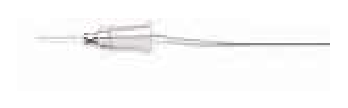
\includegraphics{./images/EEG_electrode_DEN-12SAF.eps},
  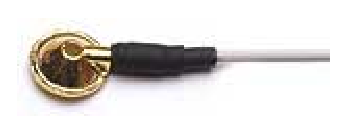
\includegraphics{./images/EEG_electrode_GH-48S.eps}}
  \caption{Sample EEG electrodes}\label{fig:EEG-electrode}
\end{figure}

Different types of electrodes with pros/cons can be used,
Fig.\ref{fig:electrode-AgCl-and-Platinum}
\begin{enumerate}
    \item crude glass electrodes (used in the early day): large size and thus
    cannot be used in many cells, i.e. mostly famouse for recording in
    squid giant axon.

    \item finer glass electrode with tips of 2-5$\mum$ diameter (Graham and
    Gerard (1946)): can be used for skeletal muscle cells.

NOTE: glass micropipettes were also starting to be
used for superfusion and application of drugs

    \item Silver/Silver Chloride electrode (AgCl coating):
     reversible but exhaustible
{\small
\begin{verbatim}
- perform well in solutions containing Chlorine
- Chlorine concentration inside the micropipette (e.g. 3M KCl)
  can be different from that in the bath (e.g. 120 mM NaCl)
  --> result into the so-called "liquid junction potential"

- If AgCl is exhausted by the current flow,
  silver ions leaking can pose many problems as it damage proteins
\end{verbatim}
}
    \item Platinum electrode:  irreversible but inexhaustible
\end{enumerate}

\begin{itemize}
  \item capacitor + resistor (leak) = phospholipid bilayer
  \item resistors with conductance = different types of ion channels
  \item electrodes (wire in circuit, which is used to transform current flows
  from electrons to ions) = liquids (in biology)
\end{itemize}

\begin{figure}[hbt]
  \centerline{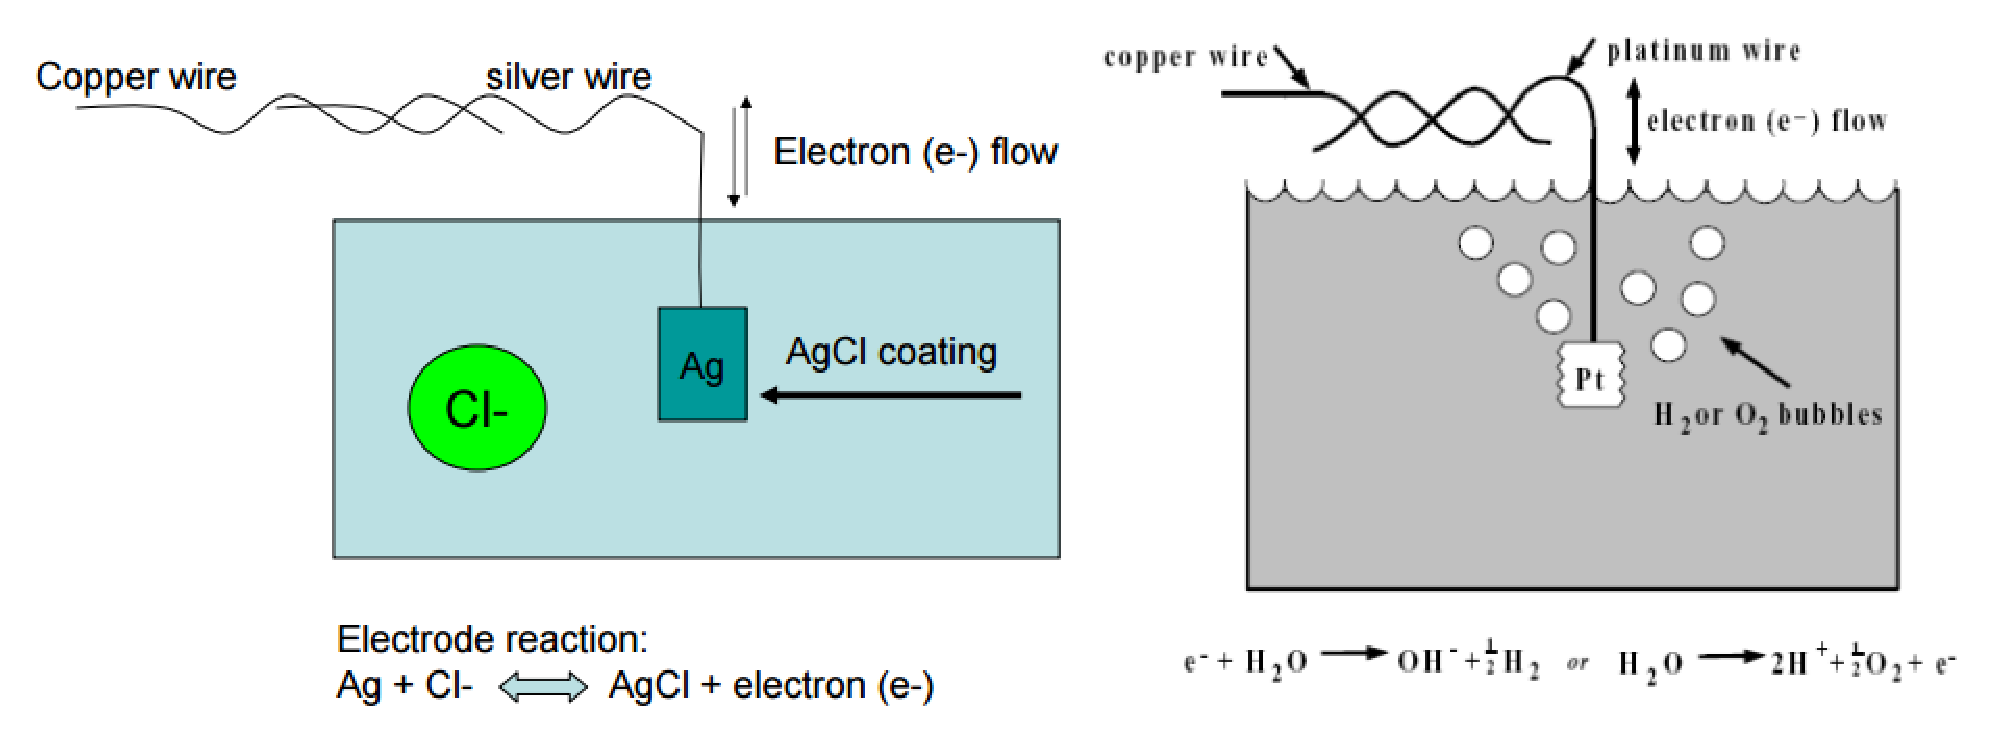
\includegraphics[height=5cm,
    angle=0]{./images/electrode-AgCl-and-Platinum.eps}}
\caption{(A) AgCl electrode; (B) Platinum electrode}
\label{fig:electrode-AgCl-and-Platinum}
\end{figure}

To measure intracellular potential, today we use microelectrode as {\it glass
micro-pipettes}\footnote{\url{http://en.wikipedia.org/wiki/Glass_electrode}}
(Sect.\ref{sec:micro-pipette}). In a landmark publication in 1976,
\citep{neher1976} introduced the using of micropipettes to form a high
resistance seals on a tiny patch of the cell membrane - which reduced
significantly the membrane area and for the first time, allowed high fidelity
recordings currents from single ion channels (Sect.\ref{sec:patch-clamp}).


\subsection{-- Micro-pipettes}
\label{sec:micro-pipette}

Micropipete is a special type of micro-electrode
(Sect.\ref{sec:micro-electrodes}) with a tip diameter $<1\mum$ and a resistance
of several mega-Ohms ($M\Omega$).

There is a compromise between the size and the resistance of the pipette as the
smaller the micro-pipette the higher the resistance. We need pipette to be small
enough so that it does not damage the cell. And we still need the resistance
small enough so that we can discriminate the small neuronal signals from noises.
Inside the micro-pipette is the solution with the ionic concentration similar to
that of the intracellular cytoplasmic and a small chlorided silver wire inside
the pipette is used to transmit the signal.

Micropipette is critical for recording, especially single channel recording
(Sect.\ref{sec:single_channel_recording}). A glass pipette with an open tip that
is very small in diameter, about $1\mum$, and is filled with electrolyte
solution (Sect.\ref{sec:electrode-electrolyte-solution}). The micro pipette is
pressed against a tiny area or patch of a cell membrane and light suction is
applied to help in the formation of a high resistance seal between the glass and
the cell membrane (Sect.\ref{sec:GigaOhm-seal}, Sect.\ref{sec:MegaOhm-seal}).

{\bf Step 1}: The choice of glass dependent upon the task is
single-channel recording or whole-cell recording.
\begin{itemize}
  \item single-channel recording: low-noise is important

  \item whole-cell recording: dynamic performance is important than the
  contribution of the pipette to the background noise
\end{itemize}


{\bf Step 2}: The choice of the electrode glass stock with a tip of optimal
geometry that is pulled into a pipet. This geometry differs between
single-channel recording or whole-cell recording.


{\bf Step 3:} The outside wall of the pipet is coated with a hydrophobic
elastomer possessing good electrical properties. This procedure is essential for
low-noise single-channel recordings but can be done much less carefully for
whole-cell recording.

\url{http://neurobio.drexelmed.edu/GaoWeb/Resources/Recording _Techniques.pdf}

\subsection{Electrolyte solution of electrode}
\label{sec:electrode-electrolyte-solution}


For intracellular recording electrodes were filled with one of the following
solutions (in mM):
\begin{itemize}
  \item potassium = Gluconate 150, HEPES 10, EGTA 3, pH 7.4 (Kay, Wong (1986))

  \item KF 120, CaC12 1, MgC1 2, EGTA 11, HEPES 10, pH 7.4. (Kay, Wong (1986))

NOTE: There is no sodium in the intracellular recording solution that Kay, Wong
(1986) used. So, this may create a larger inward current, or larger overshoot of
action potential in the recording trace.

  \item external and the internal (pipette-filling) solutions were designed to
  separate the Na + channel current (INa) from other voltage-dependent currents
  (Ogata, Tetabayashi, 1990).

The external solution contained (in mM): NaCl 100, tetraethylammonium chloride
(NMe4Cl) 25, CaCl2 1.8, CsCl 5, MgCl2 1, glucose 25, HEPES 5, and CoCl2 2.
The solution was titrated to pH 7.4 with NaOH.

The internal solution contained (in mM): caesium glutamate 125, NaCl 10, MgCl2
2.5, HEPES 5, EGTA 5, and glucose 5. The pH of the internal solution was
adjusted to 7.0 with CsOH.

The replacement of external and internal K+ with Cs+ and the presence of the
external \ce{NMe_4^+} effectively suppressed the K+ current.
The external \ce{Co^{2+}} totally suppressed the Ca2+ current.

\end{itemize}
All recordings were made at room temperature.

\subsection{-- MegaOhm seal}
\label{sec:MegaOhm-seal}

\citep{neher1976} introduced the technique (Sect.\ref{sec:patch-clamp})  to
record, for the first time, the current via a single or a few ionic channels.
A small heat-polished glass pipette is pressed against the cell membrane,
forming an electrical seal with a resistance of the order of
50 M$\Omega$ (Neher, 1978).

The high resistance of this seal ensures that most of the currents originating
in a small patch of membrane flow into the pipette, and from there into
current-measurement circuitry contained in the headstage of the pipette. The
circuit is a current-to-voltage converter
(Sect.\ref{sec:current-to-voltage-converter}).

This high resistance of the seal is important also because it determines the
level of background noise in the recordings.
Also, to reduce the dominant source of background noise, the leakage shunt under
the pippete rim between membrane and glass, the cell membrane had to be
treated enzymatically. 

\subsection{-- GigaOhm seal}
\label{sec:GigaOhm-seal}

The GigaOhm seal refers to the extremely tight contact formed by the
microelectrode attaching to the membrane, i.e. giving very low ionic current
loss, Fig.\ref{fig:pipete-seal-leaky}, and provides better results than the
traditional Mega-Ohm seal (Sect.\ref{sec:MegaOhm-seal}).
We now can obtain giga-seals on nearly every cell type we have tried.
It should be noted, however, that enzymatic treatment of the cell surface is
required in many cases, either as part of the plating procedure for cultured
cells, or as part of the preparation of single cells from adult tissues.

The high resistance of a "giga-seal" helps
\begin{itemize}
  \item reduce the noise caused by the loss, i.e. improve the quality of
  recordings

reduces the background noise of the recording by an order of magnitude, and
allows a patch of membrane to be voltage-clamped without the use of
microelectrodes (Sigworth and Neher 1980).

  \item Giga-seals are also mechanically stable, which enables whole-cell
  patch-clamp to be performed (Sect.\ref{sec:patch-clamp-whole-cell})

  \item patch patch-clamp: gently pull the membrane patch with the attached
  pipet off the cell (Sect.\ref{sec:patch-clamp-patch}).

\end{itemize}

During electrode placement, electrode resistance is monitored continuously by
applying a small voltage pulse (1-5mV, 2-10ms) to the electrode.
Once contact is made between the electrode and cell membrane, electrode
resistance spontaneously increase by 10-50\%.  To form GigaOhm seal, one applies
a gentle suction to the electrode by mouth or a small syringe.


\begin{figure}[htb]
%   \centerline{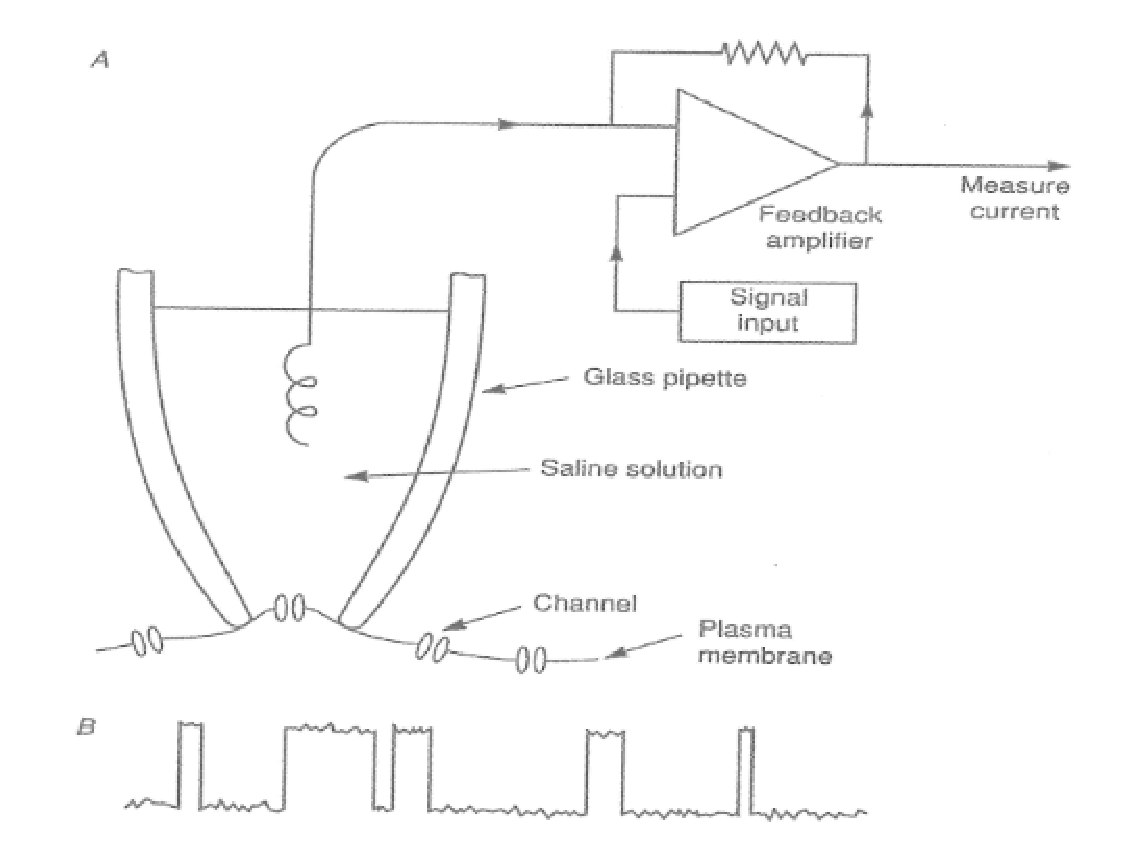
\includegraphics[height=5cm]{./images/voltage_clamp.eps}}
%   \centerline{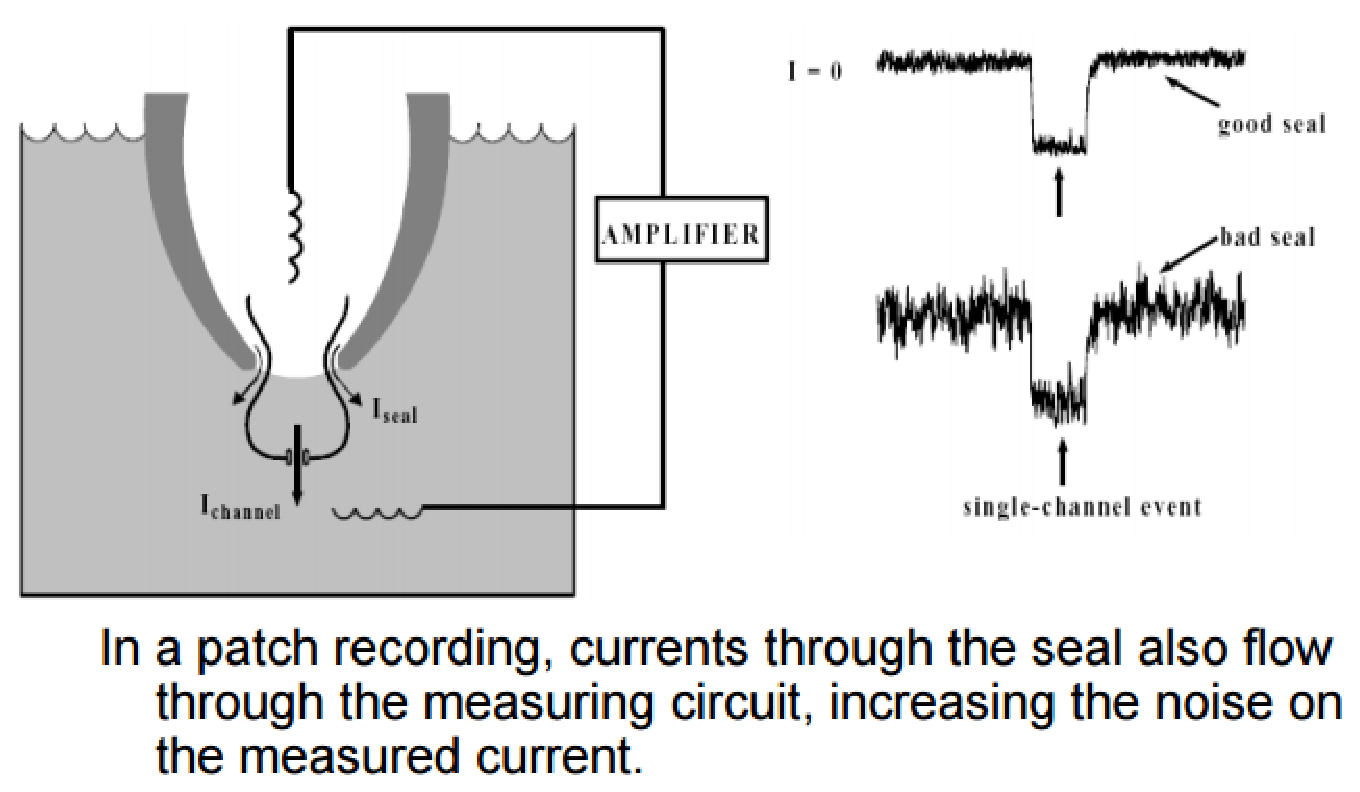
\includegraphics[height=4cm,
%     angle=0]{./images/pipete-seal-leaky.eps}}
  \centerline{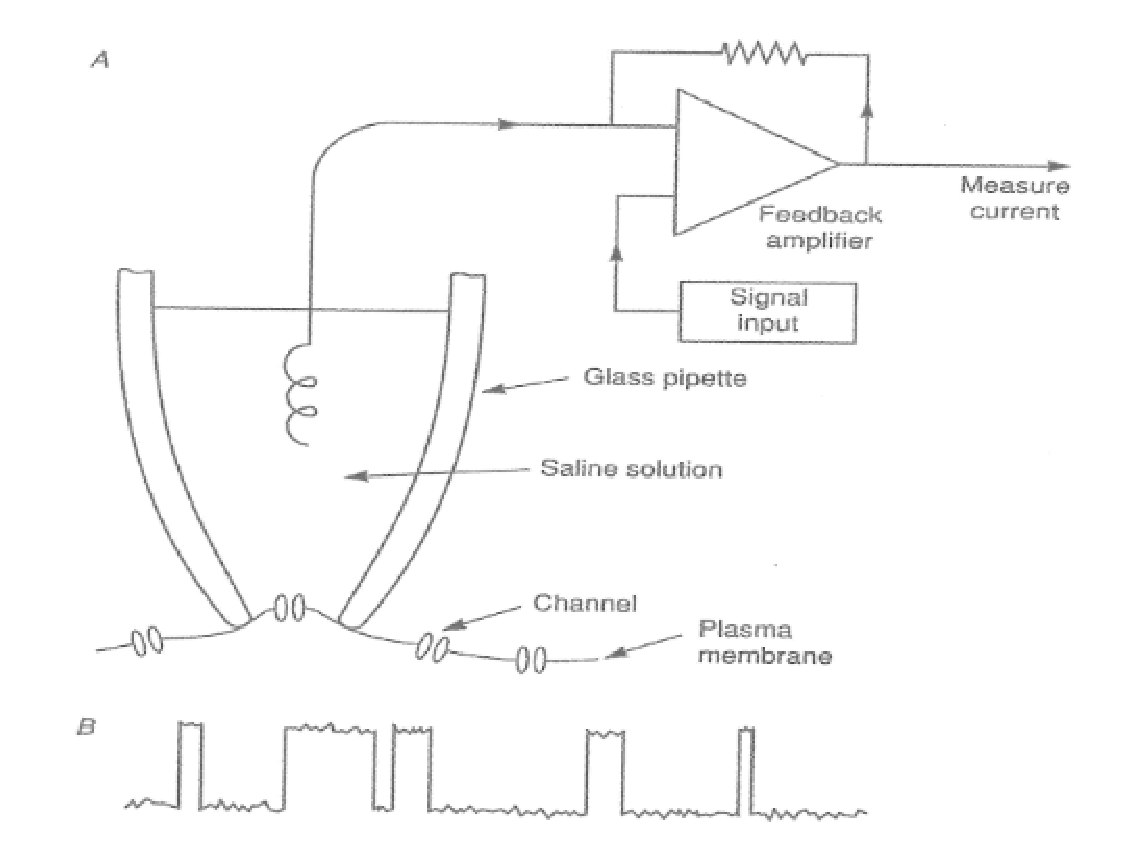
\includegraphics[height=5cm]{./images/voltage_clamp.eps},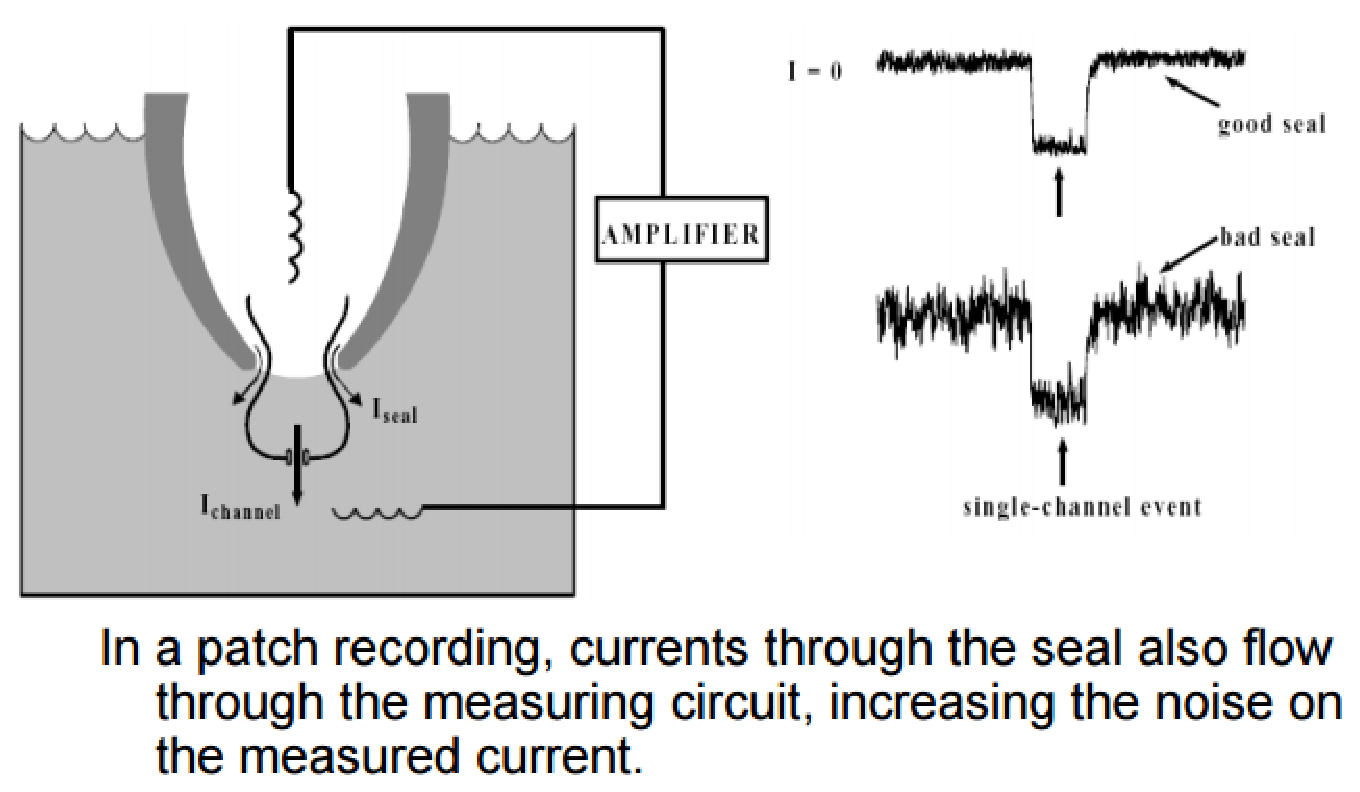
\includegraphics[height=4cm,
    angle=0]{./images/pipete-seal-leaky.eps}}
  \caption{Demonstration of patch-clamp
  technique. The current through the seal $I_\text{seal}$ also recorded as part of
the $I_\text{channel}$, increasing the noise on the measured
current. GigaOhms resistance formed between the pipette-membrane interface is
required to avoid
$I_\text{seal}$ leaky current
and is critical for the good
measurement of single-channel
current}\label{fig:voltage-clamp-measure-channel-gating}
\label{fig:pipete-seal-leaky}
\end{figure}
%, Fig.\ref{fig:pipete-seal-leaky}.

\section{Op-amp (operational amplifier)}
\label{sec:op-amp}

An operational amplifier (op-amp) is a device as shown in Fig.\ref{fig:op-amp}
that satisfy the {\bf golden rules} (properties)
\begin{enumerate}
  \item $V_\text{out} = G \times (V_+ - V_-)$ with G is the
  gain (in theory: $G \approx \infty$)

The output voltage of the op-amp is the difference between the voltages present
at the non-inverting ($V_+$) and inverting ($V_-$) inputs multiplied by the gain
$G$, assumed here to be infinite, but in reality of the order of $10^5$ or more.
This gain is not particularly useful until the output is connected back to the
inverting input in some way.

  \item inputs ($V_+, V_-$) draw no current

  \item use-cases: open-loop (i.e. amplify the signal) -
  Sect.\ref{sec:op-amp_open-loop}), closed-loop with positive or negative
  feedback (Sect.\ref{sec:op-amp_closed-loop_negative-feedback})

  Example: negative feedback (with resistance $R_f$) ensure (in theory) $V_-$
  get the same value as $V_+$, in practice; they are as close as possible
  depending the gain value.

  In the presence of the negative feedback, the output tends to displace $V_-$
  towards $V_+$.
  The larger the gain, the closer the two become; at infinite gain we can assume
  that the the two are equal.

  \item

\end{enumerate}

The purpose of an op-amp is to increase the voltage
level of a signal (to a useful or detectable level) while preserving as
accurately as possible the original waveform. Two important properties for a
good amplifier:
\begin{enumerate}
  \item  Linear amplitude response is an
important property so that the output signal is directly proportional to the input signal.
  \item A predictable and stable gain: magnitude of the gain is equal to the ratio of the output
signal amplitude to the input signal amplitude
  \begin{verbatim}
  gain = Aol = Vout/Vin
  \end{verbatim}

\end{enumerate}
They can be used to make filters, limiters,  rectifiers, oscillators,
integrators, and other devices.


\begin{figure}[hbt]
  \centerline{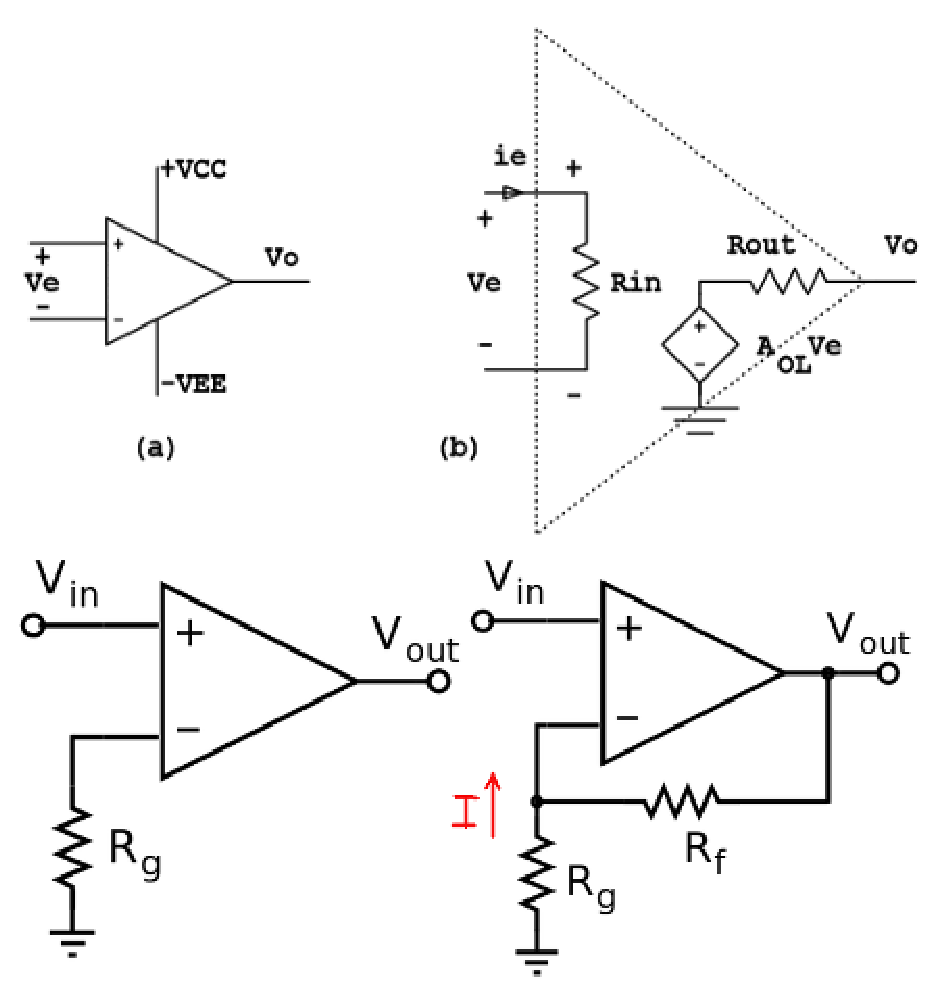
\includegraphics[height=5cm,
    angle=0]{./images/op-amp.eps}}
\caption{(a) a typical op-amp with 2 inputs + 1 output, and 2 voltage-supply
(-Vee, +Vcc); (b) a simple internal design of an op-amp; (c) usage case 01:
open-loop amplifier, i.e. one input is grounded (here, it is the inverting
input is grounded), (d) use case 02: a negative-feedback non-inverting op-amp}
\label{fig:op-amp}
\end{figure}

When using an op-amp, one input is connected with a given voltage Vin,
and the other input is grounded, Fig.\ref{fig:op-amp}.
Depending on how  we design the feedback circuit, the gain of the  output Aol is
considered as a  transfer function, which can be the combination of multiple
Aol$_i$ in a linear/non-linear way.

Op-amps require power supplies and the output voltage therefore cannot exceed
the supply voltage.
\begin{equation}
-V_\text{ee} \le V_- \le V_\text{out} \le V_+ \le +V_\text{cc}
\end{equation}
Example: for $\pm$15 V supplies, the op-amp will work
correctly in the linear operating range between, say, $\pm$13 V.
Fig.\ref{fig:op-amp}.


\subsection{- open-loop amplifier}
\label{sec:op-amp_open-loop}

An open-loop amplifier is the basic usage of an op-amp, Fig.\ref{fig:op-amp}(C):
\begin{verbatim}
 Vout = Aol * (V+ - V-) = Aol * Ve
 \end{verbatim}
 with Ve = V+ - V-.

Basically, it performs the amplification of the 'differential input', i.e.
finding the difference between two inputs  V+ (a non-inverting input) and V-
(the inverting input) and amplify the difference with a factor Aol,
Fig.\ref{fig:op-amp}

\begin{mdframed}

\verb!Aol! (open-loop gain) is typically very large (>100,000) so that even
with a small voltage difference in the input, the op-amp can drive the amplifier
output nearly to the supply voltage. The term open-loop refers to the absense of a
feedback loop from the output to the input.
\end{mdframed}

\textcolor{red}{An ideal open-loop op-amp has an infinite loop-gain Aol},
$\text{Aol} = \frac{\text{Vout}}{\text{V+ - V-}}\rightarrow \infty$; with a very
large input resistance Rin = $V_e/i_e$, and very small output resistance Rout
$\approx 0$.


\subsection{- closed-loop amplifier: positive-feedback vs. negative-feedback}
\label{sec:op-amp_closed-loop_negative-feedback}
\label{sec:op-amp_closed-loop_positive-feedback}

An open-loop op-amp itself has very high gain, but relatively poor gain
stability and linearity.

To help stabilize Vout, a feedback is often used as a powerful tool ({\bf
closed-loop amplifier}). Example: Even with zero input Vin=0, a small
time-varying noise signal do exist in the circuit. Suppose there is a small
change in Vout, indicating by an upward arrow if the change is small positive.
\textcolor{blue}{How the system stabilize itself by reducing Vout?}
The answer is: due to the feedback connection, this small change is returned
back to the op-amp input through voltage divider Rg, Rf; and increases V-, in
the case the feedback loop is connecting to V-. In turns, it will then cause a
decrease in Vout, i.e. reducing the previous positive noise in the Vout. So,
\begin{itemize}
  \item positive-feedback : amplify the change in Vout
  \item negative-feedback: remove the change in Vout
\end{itemize}

\begin{enumerate}
  \item positive-feedback ({\it positive-feedback = Vout connects a feedback
  circuit to V+ via a resistance Rf}): devices are often driven up to their
  extreme operating mode (e.g. comparator, flip-flops, oscillators, timing circuits)

%   NOTE: Vout is connected back to V+   (inverting input) via the feedback
%   circuit.

  \item negative-feedback ({\it negative-feedback = Vout connect a feedback
  circuit to V- via a resistance Rf}): devices are often in their linear mode
  (e.g.   amplifiers, linear voltage regulators (such as maintaining the
  voltage in voltage-clamp protocol), filters)

In a negative feedback op-amp, though the gain is greately reduced, it is very
stable limited only by the temperature dependence of the resistors Rg and Rf.
A close-loop {\bf op-amp} with negative feedback can be used to
make an amplifier with different desired properties
\begin{enumerate}
  \item stable gain

  \item high linearity

  \item low output impedance
\end{enumerate}

\end{enumerate}



% A negative feedback op-amp can be either non-inverting
% or inverting voltage amplifier.
% \begin{itemize}
% %  \item positive-feedback op-amp:
%
%   \item negative-feedback non-inverting op-amp:
%
% The input voltage signal Vin is applied to the non-inverting input V+ of op-amp,
% and Vout is connected back to V- (inverting input) via the feedback circuit.
%
%   RESULT: the output voltage of the op-amp closely follows that input voltage
%   Vin.
%   \url{http://www.allaboutcircuits.com/textbook/semiconductors/chpt-8/negative-feedback/}
%
%   \item negative-feedback inverting op-amp: Vout is connected back to V-
%   (non-inverting input) via the feedback circuit, and apply a voltage signal
%   Vin to the inverting input V-
% \end{itemize}

\section{Filters}
\label{sec:filter-electrical}

Basically, an electrical filter is an electronic circuit that can be designed to
modify, reshape or reject (attenuate/weaken) all unwanted frequencies of an
electrical signal and accept or pass only those signals of frequencies wanted by
the circuits designer.

So, an electrical filter filter out unwanted signals, {\bf based on the
frequencies}; as any signal is indeed the summation of components in the form of
sinusoidal signals of different frequencies.

Filters are named based on either
\begin{itemize}
  \item the components in the circuit: passive vs. active (Sect.\ref{sec:passive-filter})

Passive: it uses resistors, capacitors, and inductors.

Active: beside using those in passive filter, it also requires amplifying
elements (e.g. transitors, op-amp).

  \item frequency: low-pass, band-pass, high-pass, and band-stop

Depending on which way around we connect the resistor and the capacitor with
regards to the output signal (Vout) determines the type of filter construction
resulting in either a Low Pass Filter or a High Pass Filter.

\end{itemize}

{\bf IMPORTANT}: The reactance of a capacitor
(Sect.\ref{sec:capacitive-reactance}) varies inversely with frequency, while the
value of the resistor remains constant as the frequency changes.



\subsection{passive vs. active filters}
\label{sec:passive-filter}
\label{sec:active-filter}

Passive filters are made up of passive components such as resistors, capacitors
and inductors and have no amplifying elements (transistors, op-amps, etc) so
have no signal gain, therefore their output level is always less than the input.

An active filter use op-amp to increase the signal, i.e. gain
(Sect.\ref{sec:op-amp}).

A simple filter has an RC; more sophisticated low pass filters have a
combination of series inductors and parallel capacitors.


Passive RC filters attenuate the signal and have a gain of less than one,
(unity). It functions as a {\bf voltage divider}, e.g.
to divide its supply voltage by the ratio of R2/(R1+R2)
\begin{equation}
\text{Vout} = \text{Vin} \times \frac{R_2}{R_1 + R_2}
\end{equation}

Here, the low-pass filter or high-pass filter is constructed by replacing one of
the voltage divider resistors with a suitable capacitor as shown.


\subsection{Low-pass filter LPF (0 Hz to a cut-off frequency)}
\label{sec:low-pass-filter}

SIMPLE MEANING: A low-pass filter blocks or attenuate the frequency components
(of the signal) above a given cut-off value; so only those below the cut-off frequency is
allowed to pass through. Because of that, its other names: {\bf high-cut
filter}, or (in audio application) treble-cut filter.


{\bf ELECTRICITY}:  A low-pass filter is often built using a simple RC circuit
(resistor-capacitor). Let's review the {\bf capacitive reactance}
(Sect.\ref{sec:capacitive-reactance}). Example: first-order passive low-pass
filter (Sect.\ref{sec:low-pass-filter-first-order})

{\bf NEURON/BRAIN}: 
\begin{itemize}
  \item  most sensory information passes through primary sensory thalamic
  nuclei, however the consequence of this remains unclear. Various propositions
  exist, likening the thalamus to a gate, or a high pass filter. Here, using a
  simple leaky integrate and fire model based on physiological parameters, we
  show that the thalamus behaves akin to a low pass filter.

i.e. only input of slow frequency can drive the spiking of thalamic neurons; but
not input at high frequency.
\url{https://www.frontiersin.org/articles/10.3389/fncir.2015.00089/full}

  \item 
\end{itemize}


\subsection{-- first-order (one-pole) passive LPF}
\label{sec:low-pass-filter-first-order}
\label{sec:low-pass-filter-one-pole}


A simple first-order passive filter can be created by connecting a single
resistor (R) and a capacitor (C) in series with an input signal (Vin), and the
output of this filter (Vout) is taken from the junction of the resitor and
capacitor, Fig.\ref{fig:filter-first-order-passive}.
\textcolor{red}{Input signal goes through both R and C; but the output signal
is taken across the capacitor only}. The name means it has only 'one' reactive
component, the capacitor, in the circuit.

\begin{figure}[hbt]
  \centerline{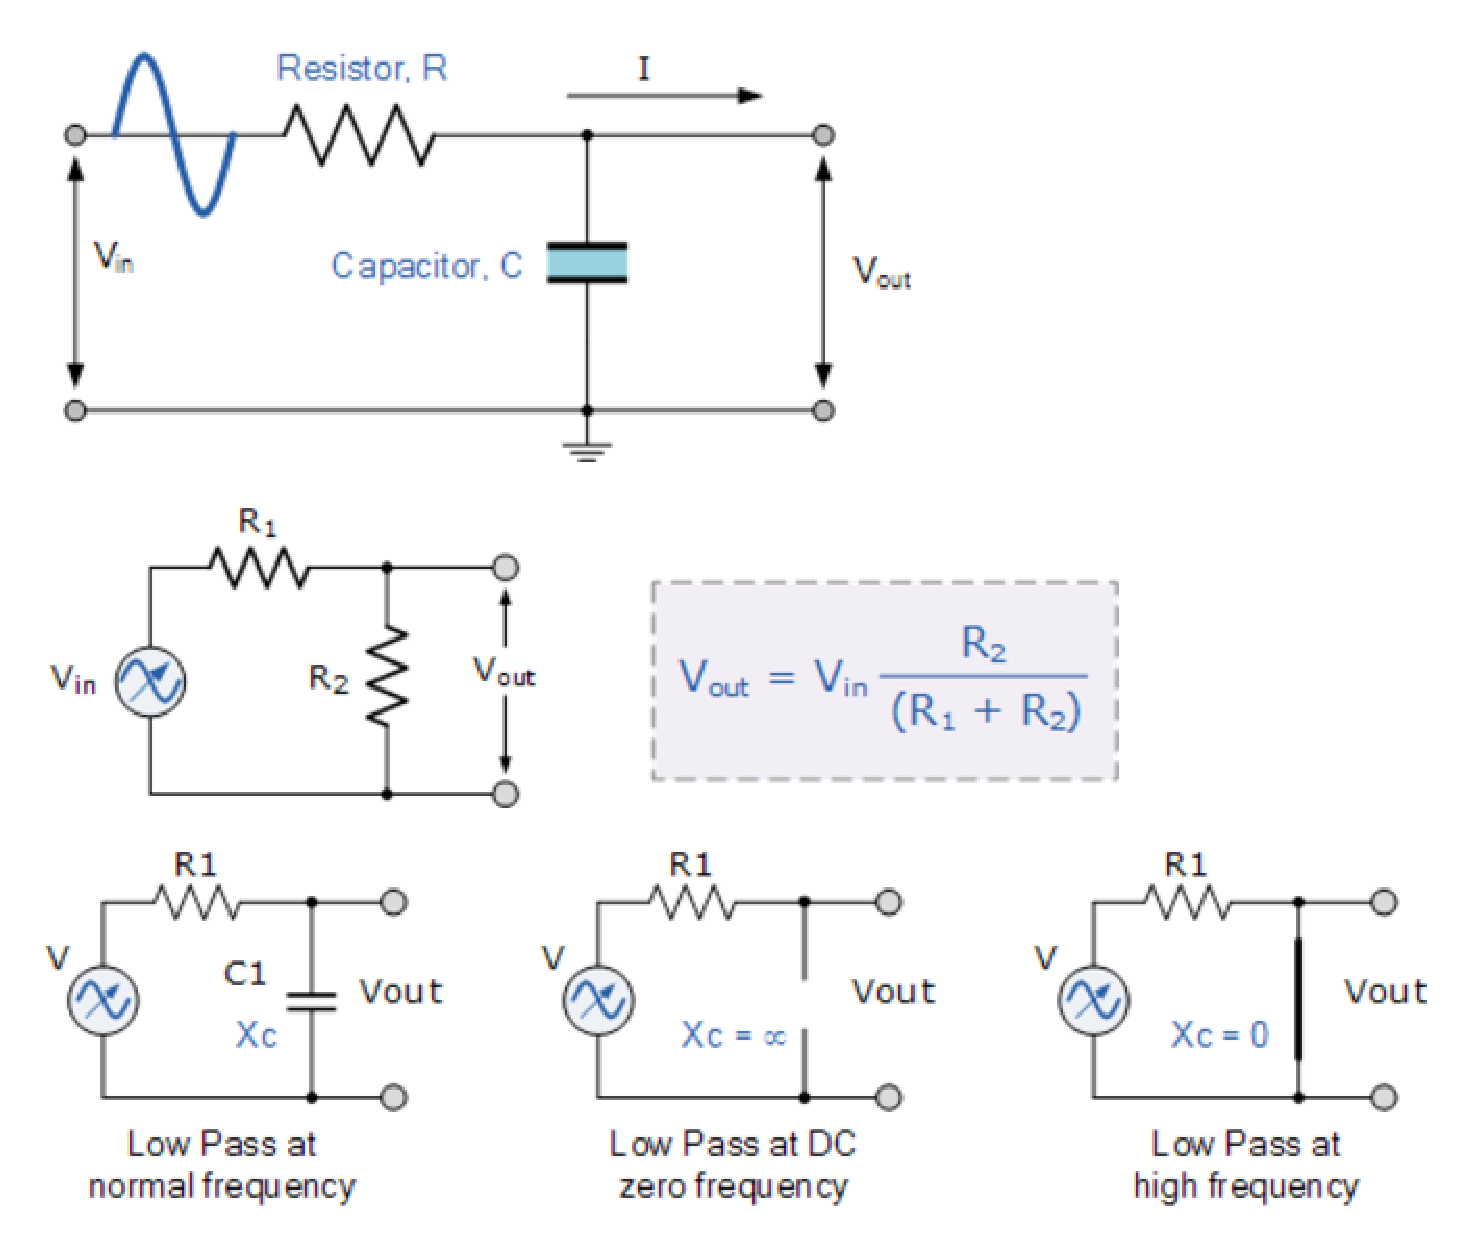
\includegraphics[height=6cm,
    angle=0]{./images/filter-first-order-passive.eps}}
  \caption{First-order passive low-pass filter}
  \label{fig:filter-first-order-passive}
\end{figure}


As the capacitive reactance Xc can change depending upon the input frequency
(Sect.\ref{sec:capacitive-reactance}), we have the following behavior of output
Vout=Vc.
\begin{itemize}

  \item  With the circuit setup in Fig.\ref{fig:filter-first-order-passive},
  low-frequency of input gives Xc will be very large compared to R of the
  resistor, i.e. voltage Vc across the capacitor will be much larger than
  voltage drop Vr which is developed across the resistor. It means, it allows
  low-frequency input to be recorded at Vout.

  \item High-frequency input Vin gives Xc much smaller than R of the resistor,
  i.e. Vc will be much smaller than compared to Vr. Remember that Vin = Vc +
  Vr; so Vin is no longer present in the output Vout=Vc.
\end{itemize}


\subsection{Band-pass filter (within certain frequency band)}
\label{sec:band-pass-filter}

\subsection{Band-stop filter (stop only within certain frequency band)}
\label{sec:band-stop-filter}

\subsection{High-pass filter (cut-off frequency to any higher freq.)}
\label{sec:high-pass-filter}


A high-pass filter is often built using a simple RLC circuit
(resistor-inductor-capacitor)

\section{Field stimulation}
\label{sec:field-stimulation}

Since tissues are usually excited by field stimulation, quite often the
threshold of excitation is reported as the number of volts injected into the
electrical field instead of the number of milivolts of membrane potential. 

Example:
\begin{itemize}
  \item  the cell is stimulated using field stimulation (e.g. Voltage-clamp
  25-30V for 2.0ms.
\end{itemize}



\section{Newer method to trigger the opening of ion channels}

To trigger the opening of ion channels: classical methods are 
\begin{itemize}
  \item tissue-level: field stimulation (Sect.\ref{sec:field-stimulation}).
  
  \item single-cell level: electrical stimulation
  (Sect.\ref{sec:voltage-clamp-techniques} or Sect.\ref{sec:current-clamp-protocol}) using an electrode.
  
\end{itemize}

However, an electrode is often not sufficiently thin and flexible to selectively
stimulate neuronal structures of interest.

\subsection{Optical stimulation}

Optical stimulation can overcome the limitation of classical electrical
stimulation (Sect.\ref{sec:voltage-clamp-techniques} or
Sect.\ref{sec:current-clamp-protocol}):

\begin{enumerate}

  \item one-photon uncaging or two-photon (2P) uncaging -
  Sect.\ref{sec:two-photon-uncaging}: more suitable for studying subcellular
  neuronal structures such as synapses.

  \item optogenetics - Sect.\ref{sec:optogenetics} : often more appropriate to
  study network properties.
\end{enumerate}


\subsection{Optogenetics}
\label{sec:optogenetics}

{\bf Optogenetics} is the application of genetic and optical techniques to
remotely control living cells (typicall neurons in the brain) in living animals
(even within freely-moving animal).
The cells must be genetically modified to express light-sensitive ion channels
or pumps.

{\it It combines optics and genetics to control and monitor the activities of
individual neurons in living tissue}, and can precisely measure the effects of
those manipulations in real-time.

The genes of which are transfected into a certain set of cells in the brain
tissues, and subsequent stimulation of their proteins causes changes in the
membrane potentials (Zhang et al. 2007; Gradinaru et al. 2010).

\textcolor{red}{Experts}
\begin{enumerate}
  \item Anatol Kreitzer -
  \url{https://gladstone.org/our-science/people/anatol-kreitzer}
\end{enumerate}

Spatially-precise neuronal control is achieved using optogenetic actuators like
channelrhodopsin, halorhodopsin, and archaerhodopsin, while temporally-precise
recordings can be made with the help of optogenetic sensors for calcium,
chloride or membrane voltage.


\subsection{Isolating ionic currents}
\label{sec:isolating-ionic-current-components}

Four methods of current isolation are commonly used to isolate voltage-activated
ionic currents:
\begin{enumerate}
  \item \textcolor{red}{kinetically}: based on the time-scale of channel
  activation and inactivation of different kinds of ion channels.

Example:
\begin{itemize}
  \item  Na+ currents typically activate within 200-300 $\mu$sec and inactivate
completely within 2-5 msec.
  \item K+ currents may take several msec to activate, and often inactivate
slowly, if at all.
\end{itemize}

Simple current isolation (mainly to study the
current amplitudes) can thus be accomplished by studying whole-cell
currents at different time points following stimulation.

  \item \textcolor{red}{current subtraction via stimulus protocols}:
  Voltage-dependence of the steady-state activation and inactivation
of currents often allows selective activation of subpopulations
of ion channels

Example:
\begin{itemize}
  \item Isolate Ca-low vs. Ca-high currents: voltage steps originating from
  different holding potentials can separate low-threshold vs. high-threshold $\Ca$ currents

  \item Isolate KA current vs. Kdr current: Depolarizing voltage steps applied
  from very negative holding potentials (e.g., -110 mV) can activate both
  transient "A" type (KA) and delayed-rectifying (Kd)
K+ currents. Voltage steps applied from a more positive holding potential (e.g.,
-50 mV) will completely inactivate all KA channels while not affecting Kd
activity, Fig.\ref{fig:KA-current-Kdr-current}

%  \item
\end{itemize}


  \item \textcolor{red}{isolation solutions}: dialysis of cytoplasm with patch
  pipet contents occurs rapidly after whole-cell configuration is achieved, thus
  allowing for manipulation of internal ionic concentrations.

Example:
\begin{itemize}
  \item to block K+ channels: replacing pipet KCl with impermeant Cs+ or
  N-methyl-D-glucoronate (NmDG) $\rightarrow$ isolate $\Na$ currents

  \item  acetate,
glucoronate, or isothionate can each be substituted for Cl- ions

  \item tetramethyl-ammonium chloride (TMA-Cl) can be substituted
for Na+ ions
\end{itemize}
It has even been reported that the contribution of one ion-channel population
can be determined by replacement of all but the desired ion with glucose or sucrose.


  \item \textcolor{red}{current isolation Via Pharmacology}: natural toxins and
  synthetic pharmacological agents
exist that can be used to reduce or eliminate specific voltage-activated ion
channel activity,  Tab.\ref{tab:ion-channel-blockers}.

\item
\end{enumerate}



\subsection{Digitize data}
\label{sec:digitize-data}

The analog output of the amplifier
(Sect.\ref{sec:patch-clamp-electronic-component}) is typically amplified to make
effective use of the dynamic range, e.g. A/D converter translates to an
amplification range of -10V to +10V.

At the same time, signals are filtered (e.g. Bessel filter).
The cell and electrode are essentially a single-stage RC filter, due to RC
component of cell membrane-series resistance combination.

As the single channel current is typically too small, an amplifier is often
used.   Suppose the amplifier can amplify the signal 1000 times (i.e. 1000
mV/pA). These voltages are then recorded (by using an oscilloscope, a chart
recorder, frequency-modulated magnetic tape...)  for display purpose, or for
further analysis. Finally, for permanent storing purpose, the recorded data need
to be digitalized into 0s and 1s; which requires an analogue-to-digital (AD)
conversion, the preprocessing of data (filter, noise removal, compressor...).
The raw data is in analog, but we can only store them in digitized form. This
requires the sampling using AD converter. AD converters, however, has a sampling
limit.



\begin{framed}

  AD converter has only a limited sampling rate (e.g. 50-200 kHz/one channel),
  i.e. 20$\mus$ - 5$\mus$. It means it cannot detect event shorter than 5$\mus$.
  Interpolation is necessary when the original signal is sampled relatively
  sparse.

  Also, AD converters accept Voltage in the
  range $\pm 10$V, with maximum $\pm 10.24$ V. The Voltage should span
  as much as possible in this range to increase the resolution. A
  quantity, {\bf dynamic range}, is used to measure the efficient use
  of an electronic device (AD converter, or amplifier).

\end{framed}

Due to the limit of Voltage input of the AD converter; the
  maximum current can be detected is $\frac{10\times 10^3
    (mV)}{1000
    mV/pA}
  = 10 pA$. If the minimum signal can be detected is $10$ fA, the
  dynamic range is $(10-(-10)) \log (\frac{10 pA}{10 fA}) = 60$ dB
  (decibels).

As the measurement is never noise-free, we need to consider the nature of
errors, noise when measuring the data and  discuss how to improve the
signal-to-noise ratio (Sect.\ref{sec:noise-analysis}) using noise removal
(Sect.\ref{sec:noise-removal}).

Next, we do {\it event detection} (Sect.\ref{sec:event-detection}), and then
from that the series of dwell-time in open and close states are estimated.
Based on the series of open dwell-time and closed dwell-time, we can estimate
build the histogram of dwell-time in open state, and closed-state,
respectively. Also, the mean dwell-time in open and closed state can also be
estimated (Sect.\ref{sec:dwell-time}).

\textcolor{red}{Example}: As shown in Fig.\ref{fig:GlyR_dwelltime}, the data was
filtered at 5 kHz, giving S/N=19. In both cases, the final time resoltuion was
15$\mus$. The experimental histogram was fitted by mixtures of exponentials
using {\bf EKDIST program}
\footnote{\url{www.ucl.ac.uk/Pharmacology/dcpr95.html}}. Here, we often use
log-scale axis, to cover a wide range
(Sect.\ref{sec:dwell-time-histogram-linear-y-log-x}).

\begin{figure}[hbt]
  \centerline{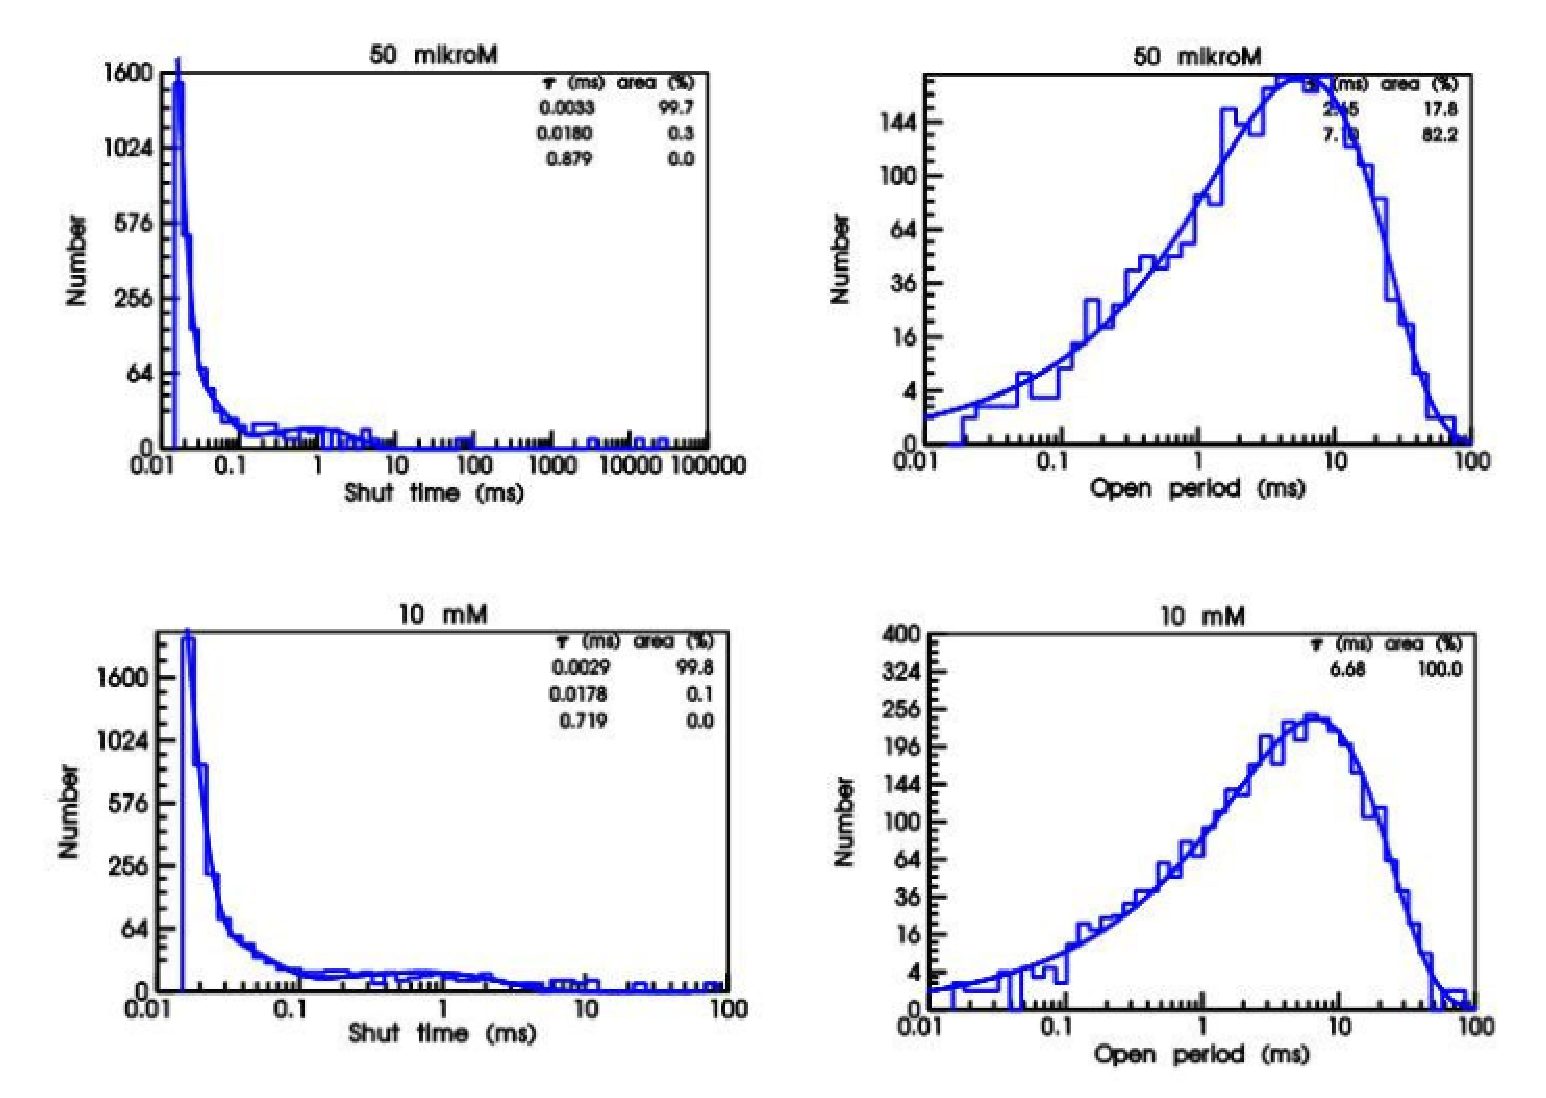
\includegraphics[height=5cm,
    angle=0]{./images/GlyR_dwelltime.eps}}
  \centerline{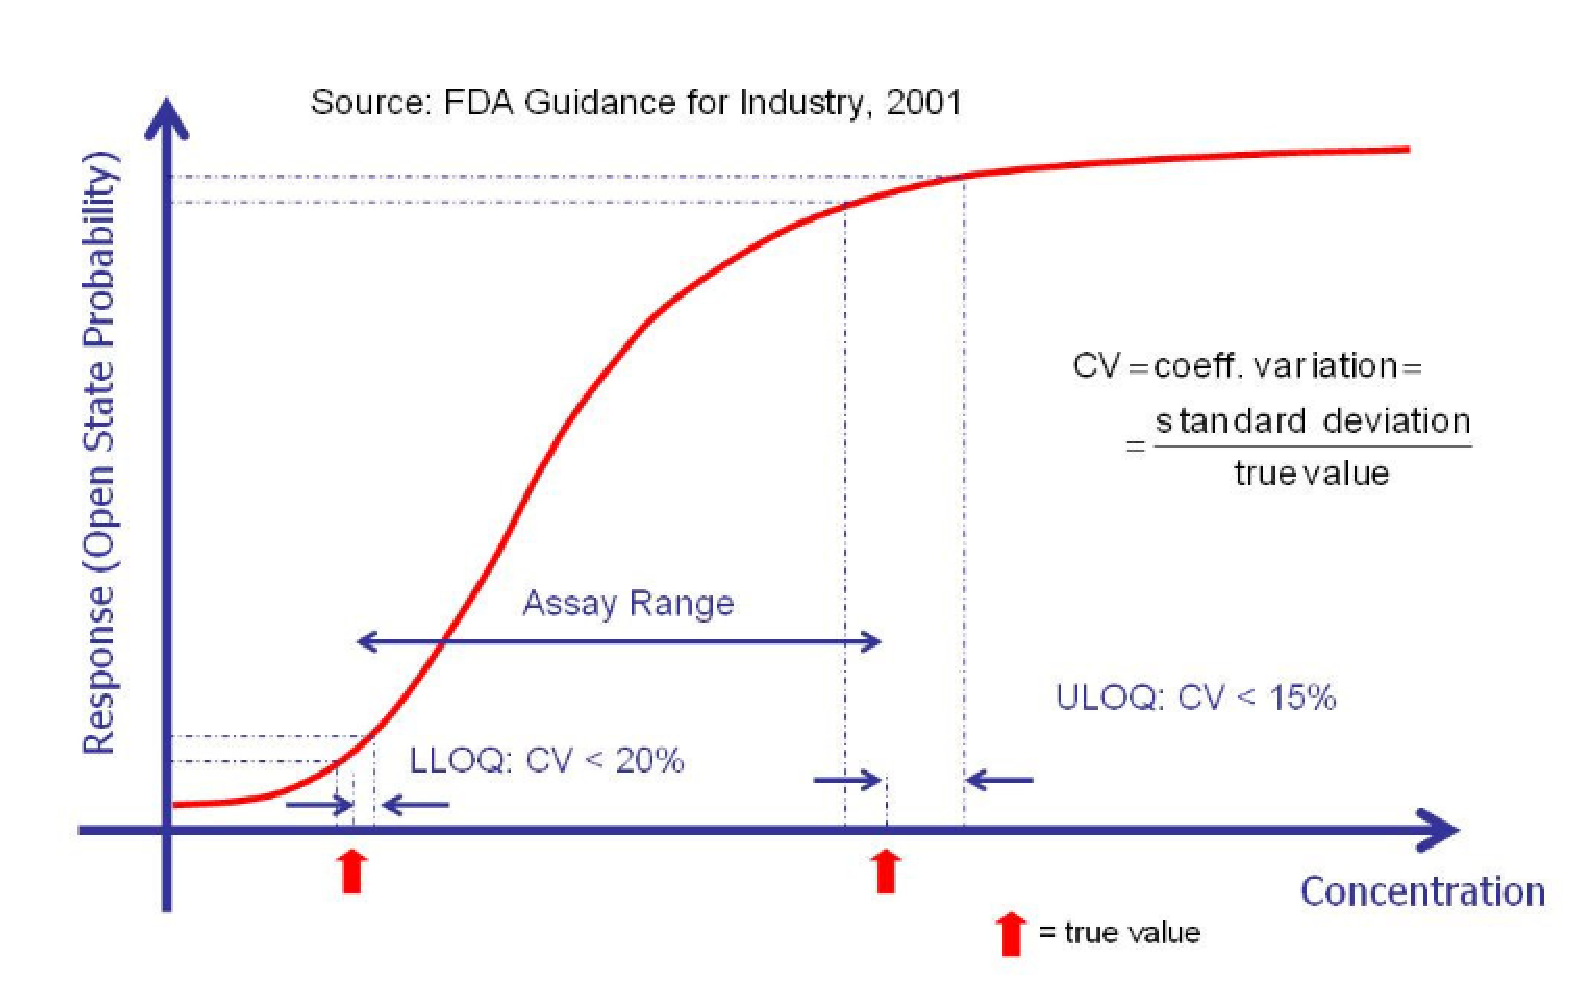
\includegraphics[height=5cm,
    angle=0]{./images/concentration-response_curve.eps}}
  \caption{Dwelltime (left: shut, right: open) distribution at two different
  concentration of Glycine: above: 50$\muM$ and below: 10mM; (B)
  Concentration-reponse curve}
\label{fig:GlyR_dwelltime}
\end{figure}

Using EKDIST, we have two shut-time components and opentime components, Table
\ref{tab:dwelltime_GlyR} \citep{lodesani2008}. This is, however, only an
empirical fit of the distribution with no kinetic models taken into account. To
realise the parameter for a given Markov-chain model, we need to use {\bf HJCfit
program} \footnote{\url{www.ucl.ac.uk/Pharmacology/dcpr95.html}}.

\begin{table}[hbt]
\begin{center}
    \begin{tabular}{lcccc}
        \hline
     & \multicolumn{2}{c}{50$\muM$} & \multicolumn{2}{c}{10mM} \\
     & tau (ms) & area(\%) & tau (ms) & area(\%) \\
shuttime & 0.0033 & & 0.0029 &  \\
    & 0.018 & & 0.0178 & \\
opentime & 2.65 & & & \\
	& 7.10 & 82.2 & 6.68 & 100 \\
    \end{tabular}
\end{center}
\caption{Dwelltime of GlyR}
\label{tab:dwelltime_GlyR}
\end{table}

To estimate the kinetic rate constant from data published in steady-state
conditions, HJCfit software need to be used. It basically maximum the likelihood
of an entire sequence of apparent open and shut times. The input is the Markov
model with the transition rates are free parameter. Since it's impossible to
know the data from a single channel, only data from intra-burst and
intra-cluster periods are analyzed, as they are being quite sure from the
activity of the same channel. Another input is the $t_\text{crit}$ the
critical shut time length, so that every burst (cluster) is contained between
shut period longer than $t_\text{crit}$.



\chapter{Extracellular recording}
\label{chap:extracellular-recording}

NOTE: extracellular recordings can normally only pick up fast electrical events,
like action potentials, but fail in case of slower, graded voltages, such as
receptor potentials or synaptic potentials.

To understand the activity of individual neurons and how that activity 
contribute to neuronal circuits, we use extracellular recording (which focus on
neuron's AP as the 'code').

LIMITATION:
\begin{enumerate}
  \item  at the membrane level: subthreshold events, such as synaptic potentials
  that might influence the cell's excitability, remain hidden.

Recording subthreshold potentials requires an intracellular or membrane level
approach; which can be done more easily in {\it in vitro} preparations, rather
than in whole animal.

  \item at the neural circuit level: single-unit extracellular
  electrode samples activity of only one or a few neurons

This can be a limitation to see the functioning of a large neuronal ensemble or
circuit with this approach. This requires multi-unit electrode recordings
  
\end{enumerate} 


e.g.
  LFP - Sect.\ref{sec:LFP})

\section{1. Extracellular recordings (voltage: microVolt $\mu$V)}
\label{sec:extracellular-recording}

\section{1.a. Extracellular single-unit recordings }
\label{sec:extracellular-recording-single-unit}

\section{1.b. Extracellular multiple-unit recordings }
\label{sec:extracellular-recording-multiple-unit}


\chapter{Trans-membrane recording (whole-cell)}
\label{chap:voltage-clamp-whole-cell}

Trans-membrane recording is needed when we need to characterize the ion channels
that regulates the dynamics of trans-membrane potential of a cell.
Typically, the recording is ionic current across the membrane and is done via
voltage-clamp technique. The technique is divided into 2 parts
\begin{enumerate}
  \item whole-cell level recording: this chapter

  \item patch-clamp recording (a few channel or single-channel):
  Chap.\ref{chap:voltage-clamp-whole-cell}
\end{enumerate}

\section{Current-clamp (record voltage)}
\label{sec:current-clamp-protocol}
\label{sec:transmembrane-potential-recording}
\label{sec:membrane-potential-recording}

The transmembrane potential $V_m$ of an excitable cell is recorded using
current-clamp technique.
Its other names: {\bf bridge} recording, {\bf voltage-follower} recording.

A voltage is recorded by having electrodes at 2 locations.
It uses an electrode intruded the membrane into the interior of the cell, which
introduces several artefacts into the recording. Suppose the recorded value is
$V_p$, while the truth 'unknown' value is $V_m$.
\begin{itemize}

  \item  The transmembrane voltage Vm is the voltage different caused by current
  passing through the RC circuit (C = capacitance caused by the phospholipid
  bi-layer as a capacitor; R = the resistance caused by ionic channels)

The electrode has a resistance, $R_e$; as the resistance is in series to the RC
circuit, it is also called series resistance $R_s = R_e$
(Sect.\ref{sec:series-resistance}).

  \item \textcolor{red}{Errors introduced by electrode}:
  However, the electrode is not completely sealed, as it
  needs a tiny hole to inject current.  So, when we pass an injected
  current throuth the tip of the electrode, which is in serial to the circuit,
  the recorded potential  $V_p = V_m + V_\text{loss}$.

%Since the micropipette is intracellular, changes in Vm are included in Vp
% \begin{equation}
% V_p = V_m + V_\loss
% \end{equation}

The voltage loss via the tip of the electrode
is 
\begin{equation}
V_\text{loss} = R_e \times I_p  = R_s \times I_p
\end{equation}
with $I_p$ is the injected current
(clamped current).

Clearly this error will be zero if no current is injected; otherwise, it can be
minimised by using large electrodes containing highly-conductive solution (which
will give a low resistance).

So, a correction is needed to ensure $V_p$ is as closed as $V_m$ as possible.
This voltage error is relatively easy to correct for, since we (and
the ampliffier) know the injected current $I_p$, and the series resistance
$R_e$ can be estimated (Sect.\ref{sec:series-resistance}). A correction is done
using {\bf bridge balance} - Sect.\ref{sec:bridge-balance}.


Because of that, the value recorded is $V_p$ which is not exactly the same as
the 'unknown' true value $V_m$, Fig.\ref{fig:current-clamp}. Often, a second
electrode is used to adjusted the error introduced (as mentioned below) and to
give 'true' reading of $V_m$.

   \item \textcolor{red}{There can be a maximum current (few nano-ampere nA) can
   passthrough the electrode}, i.e. $I_p < I_\max$.

Typically glass microelectrodes have a very non-linear current-voltage relation,
and often the response may saturate (i.e. no larger currents can be pushed
through) with currents of only a few nA's; this of course depends on the
resistance and the other properties of the electrode tip.

\end{itemize}


Whole-cell patch-clamp techniques are widely used to measure membrane currents
from isolated cells. While suitable for a broad range of ionic currents, the
{\bf series resistance (Rs) of the recording pipette} limits the bandwidth of
the whole-cell configuration, making it difficult to measure rapid ionic currents.

There have different methods proposed to compensate Rs to improve the bandwidth
\begin{itemize}
  \item Sherman, Shrier, Cooper (1999)
\end{itemize}


\subsection{applications}
\label{sec:voltage-recording}

\textcolor{red}{Example appliations of current-clamp}:
\begin{enumerate}

  \item to measure resting potential, when there is zero current injection or
  other perturbation - Sect.\ref{sec:resting-potential}.

  \item to measure voltage change caused by leak current - from that the
  conductance of leak current is estimated - Sect.\ref{sec:leak-current}.

  \item  to measure voltage change caused by currents at synaptic spine,
  i.e. such membrane potential change is called postsynaptic potential (PSP) -
  Sect.\ref{sec:postsynaptic_potential})

  By applying a known constant (or time-varying) current, we can mimics the
  current produced by a synaptic inputs, and then we measure PSP.

%  , action potential and resting potential.

\end{enumerate}

\subsection{-- estimate resting membrane potential}
\label{sec:resting-membrane-potential-estimation}

\subsection{-- estimate membrane leak current}
\label{sec:leak-current-estimation}
\label{sec:leak-conductance-estimation}

\textcolor{red}{Explain the estimation of membrane leak current}: As shown in
Fig.\ref{fig:current-clamp}, the electrode (with resistance $R_e$ -
Sect.\ref{sec:electrode-resistance}) is penetrated into the cell; along with a
parasitic capacitance $C_p$ (Sect.\ref{sec:parasitic-capacitance}).  During a
step current injection controlled by current source $I_p$, the current gets into
the soma and then flow via 2 pathways:
\begin{enumerate}
  
  \item via the phospholipid bilayer and the transmembrane proteins (as
  represented by a capacitor $C_m$ and resistance $R_m$), causing a rise in
  transmembrane potential with {\bf membrane time constant} $\tau_m = R_m C_m$.

  \item via the electrode, i.e. the loss voltage $V_\text{loss}$ (see above)

\end{enumerate}

So, under the assumption that no ionic channel is available (or opening), then
estimating surface area can give us $C_m$ (with the assumption specific
membrane capacitance $\Csc = 1 \muF/$cm$^2$). Then, looking at the voltage
trace, we can estimate the time constant $\tau_m$.  Using those two values,
it helps to tell membrane resistance $R_m = \frac{\tau_m}{C_m}$
(Sect.\ref{sec:membrane-resistance}).

Finally, the leak conductance: $G_\leak = 1/R_m$
(Sect.\ref{sec:leak-current}).


\begin{figure}[hbt]
  \centerline{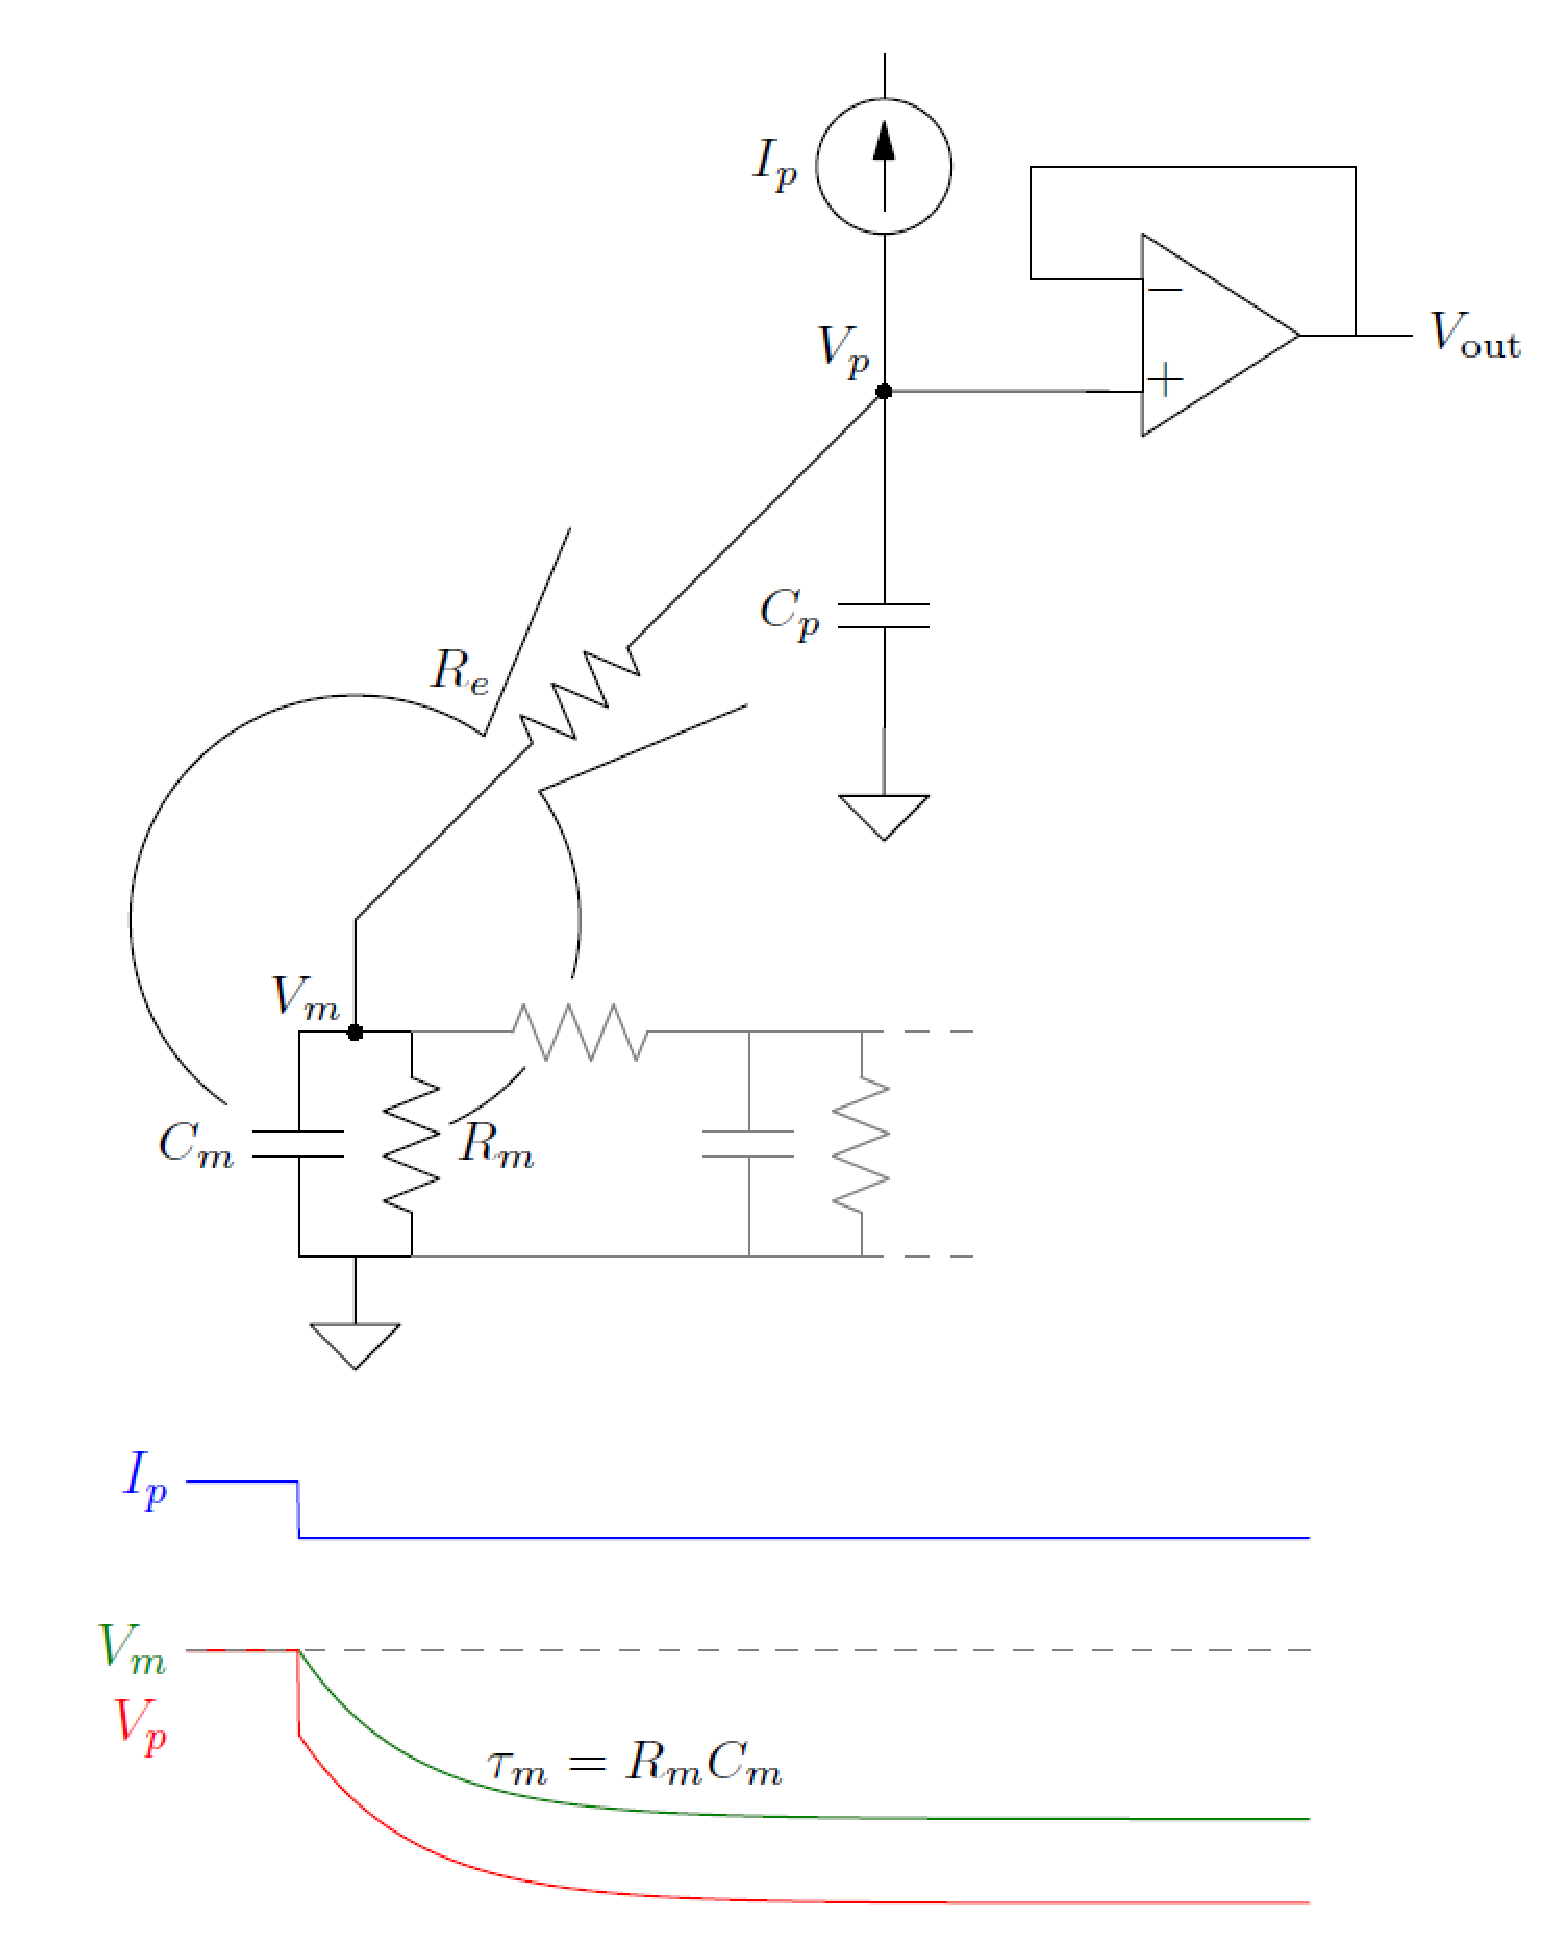
\includegraphics[height=5cm,
    angle=0]{./images/current-clamp.eps},
    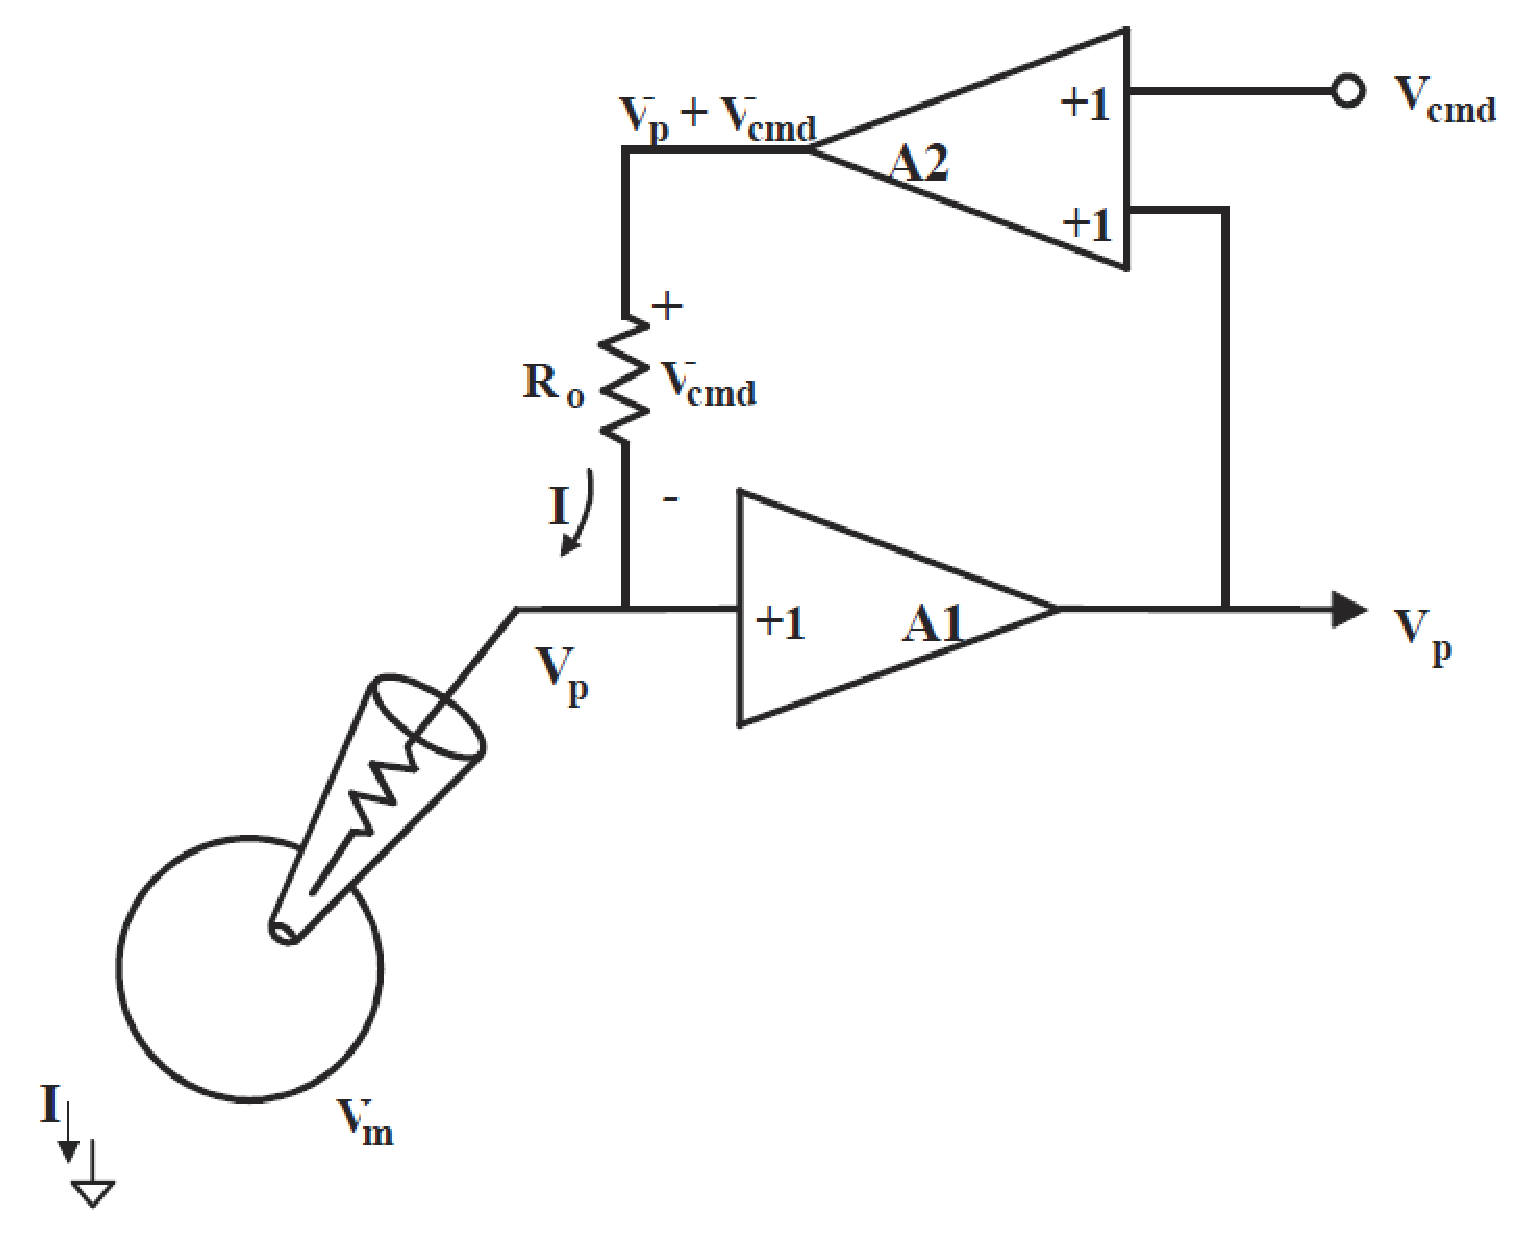
\includegraphics[height=5cm,
    angle=0]{./images/current-clamp-current-source.eps}
    }
\centerline{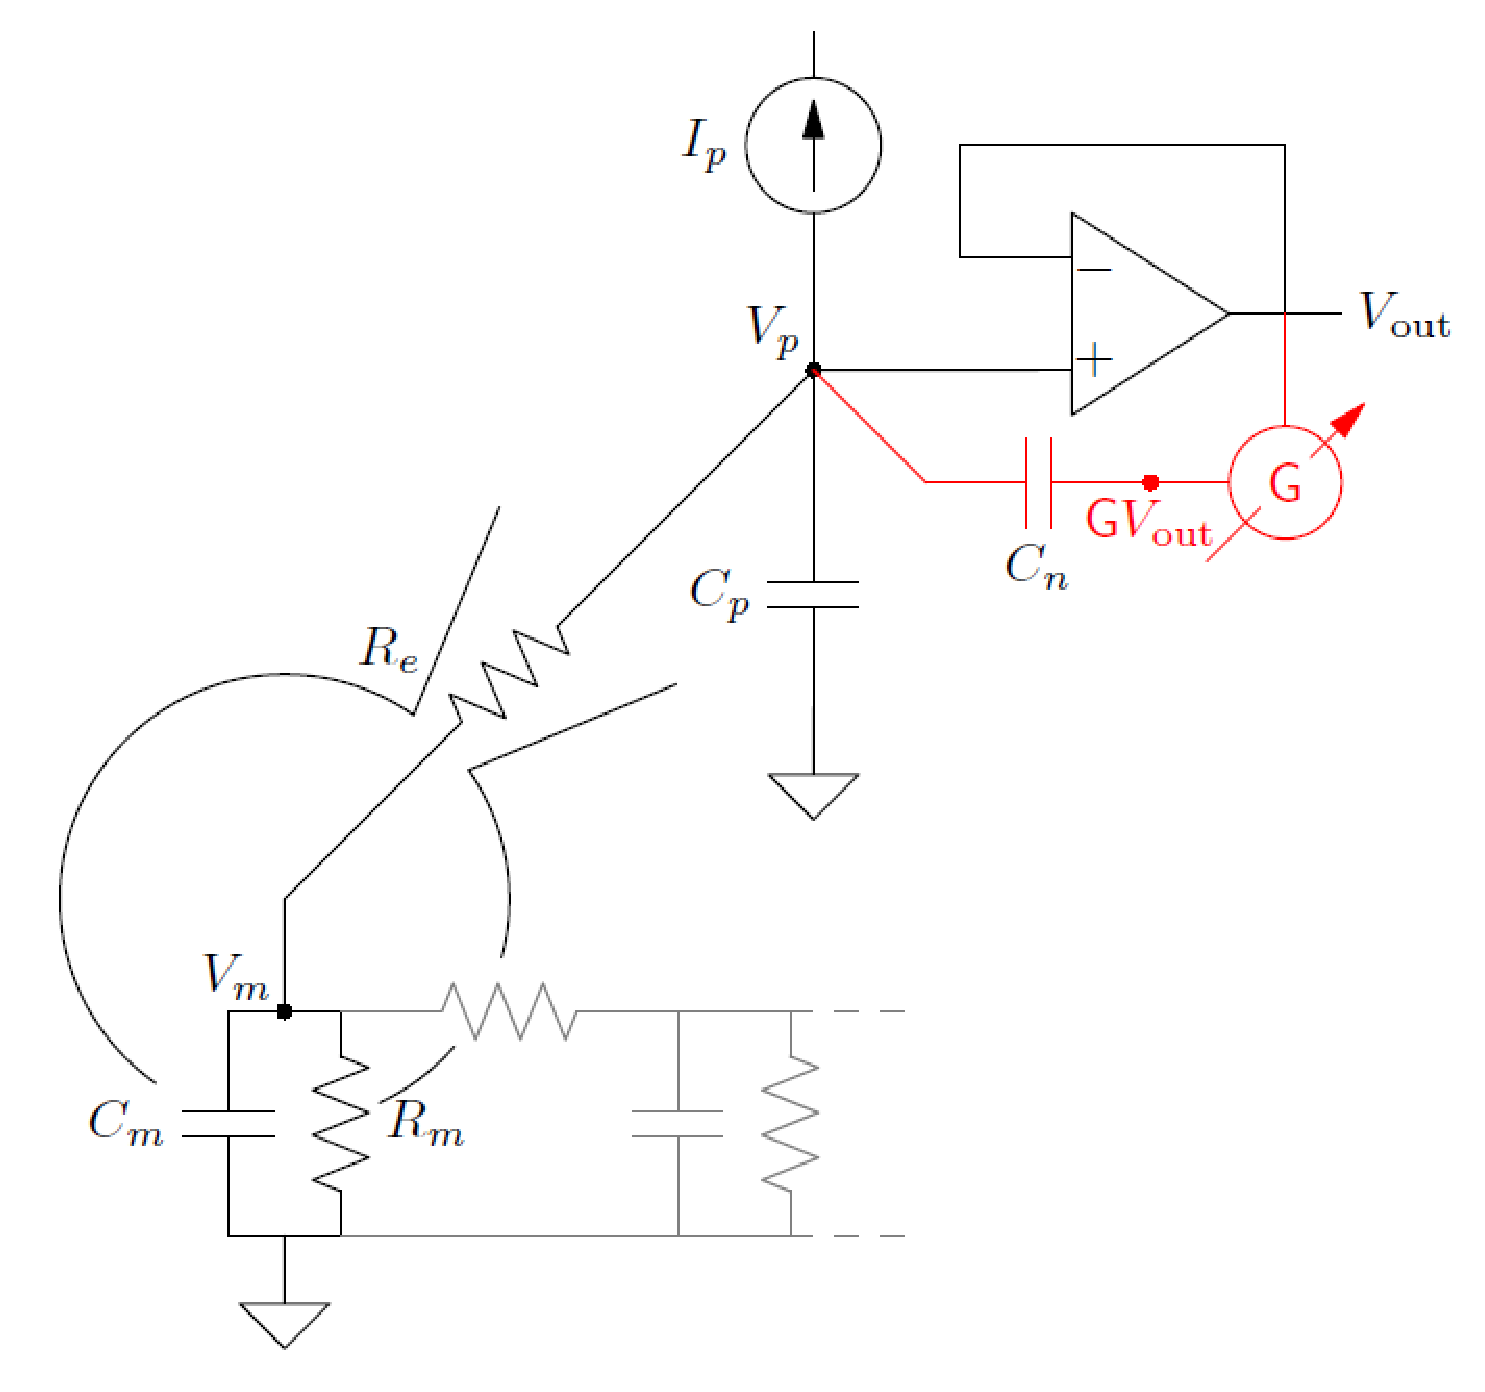
\includegraphics[height=5cm,
    angle=0]{./images/current-clamp-capacitance-neutralization.eps}}
  \caption{Voltage recording using current-clamp protocol: recorded value $V_p$
  which is aimed to reflect the value of $V_m$. A current $I_p$
  is the injected into the cell via an electrode of resistance $R_e$.
  An amplifier (is needed to record the signal) as an Op-amp with
  negative-feedback (Sect.\ref{sec:op-amp_closed-loop_negative-feedback}) ensure
  $V_\out=V_p$. However, as you will learn in the text that $V_p$ is not
  exactly the same as $V_m$ due to voltage loss $V_\text{loss}$ or
  $V_\text{err}$. (B) {\bf High quality current source}: a second op-amp is used
  with two input: $V_\text{cmd}$ and $V_p$. This ensures the voltage out of
  op-amp A2 is always $V_\text{cmd}$ regardless of $V_p$; and thus the input
  current source is always $I_p = V_\text{cmd}/R_p$ regardless of $V_p$.
  (C) {\bf Capacitance neutralization}: {\bf G} is the amplifier; a positive
  feedback circuit (in red) is added, which injects an amplified version of the
  output back into the input via a capacitor.}
  \label{fig:current-clamp}
\end{figure}

\clearpage 

\subsection{parasitic capacitance (stray capacitance)}
\label{sec:current-clamp-stray-capacitance}
\label{sec:parasitic-capacitance}

The parasitic capacitance, or stray capacitance is an unavoidable and usually
unwanted capacitance that exists between the parts of an electronic component or
circuit simply because of their proximity to each other.



The capacitor of {\bf parasitic capacitance} $C_p$ arises from the capacitance
between the electrode  filling solution and the bath saline combined with some
unavoidable capacitances associated with the headstage and its electronics.
Stray capacitances are often of the order of a few picofarads, but much larger
or smaller values are possible

 Remember that a capacitor requires current flow to change its voltage.
Thus, in order to record a change of membrane potential at the amplifier,
the parasitic capacitance must be charged.


\subsection{current source}
\label{sec:current-clamp-current-source}



\subsection{bridge balance: compensation circuit to correct
voltage drop}
\label{sec:bridge-balance}
\label{sec:current-clamp-bridge-balance}


The voltage loss $V_\loss$ (Sect.\ref{sec:current-clamp-protocol}) is corrected
by adding a circuit that (1) can generate a signal that is proportional to the
product of the micropipette current $I_p$ and the micropipette resistance $R_e$;
(2) this signal is then subtracted from the buffer amplifier output (to separate $V_m$
component from $V_p$). 

The technique is called {\bf Bridge Balance} as in the
early day, a resistive circuit known as a Wheatstone bridge (a resistor network)
was used to achieve the given goals with $R_v$ adjusted until 'balance', i.e. no
voltage between C and D, Fig.\ref{fig:Wheastone-bridge} (see Daavid J.
Aidley's book - The Physiology of Excitable Cell, page 42) -
Sect.\ref{sec:Wheatstone-bridge}.
% https://books.google.com/books?id=3JgC_rE8ZVwC&pg=PA42&lpg=PA42&dq=In+1939,+Cole+and+Curtis+use+a+Wheatstone+bridge&source=bl&ots=-TmGqNzorw&sig=j2zCzgb0DhB_qHXB-5sYzaizI3M&hl=en&sa=X&ved=0ahUKEwiI_YOZ6sfVAhWITCYKHQTPDB4Q6AEITzAH#v=onepage&q=In%201939%2C%20Cole%20and%20Curtis%20use%20a%20Wheatstone%20bridge&f=false

\begin{enumerate}
  
  \item In Fig.\ref{fig:Wheastone-bridge} for DC circuit: 
  the two known fixed resistance $R_1$ and $R_2$ are used; and $R_3=R_v$ is a
  known variable resistance.
  
  $R_v$ is altered until there is no voltage between C and D, i.e. the bridge
  is called to be balance, i.e. 
  \begin{equation}
  R_1/R_2 = \frac{R_x}{R_v}
  \end{equation} 

As we know $R_v$; the formula enable us to find $R_x$.

  \item for AC circuit, Fig.\ref{fig:Wheastone-bridge}(B): a similar method can
  be used to find the unknown impedance Z.
  
  If the two fixed resistance $R_1$ and $R_2$ are equal, then the bridge is
  balanced when the variable resistance $R_v$ is equal to $R_x$; and the
  variable capacitance $C_v$ is equal to $C_x$.
  
\end{enumerate}

\textcolor{red}{NOTE: All modern micropipette ampliffiers use a different
implementation using op-amps}. Operational amplifier circuits are used to
generate the subtraction, but the name has persisted. There are several ways to
set the bridge balance
\begin{enumerate}
  \item A commonly used technique: brief repetitive pulses, e.g. 5 nA 2ms pulse
  is applied to a 50 M$\Omega$ electrode

IN THE BATH: apply brief repetitive pulses of current to the micropipette while
it is immersed in the preparation bath. The Bridge Balance control is advanced
until the steady-state pulse response is eliminated,
Fig.\ref{fig:bridge-balance}(B). At this point, the circuit is balanced and the
micropipette resistance can be read from the calibrated readout of the Bridge
Balance control.

The same technique can even be used after the micropipette has penetrated the
cell.

  \item
\end{enumerate}
It is important that the micropipette resistance be constant. Clearly, if the micropipette
resistance varies as the current flows there will be no unique setting of the Bridge Balance
control and the measurement will include an artifact due to the variable voltage drop
across the micropipette.

\begin{figure}[hbt]
  \centerline{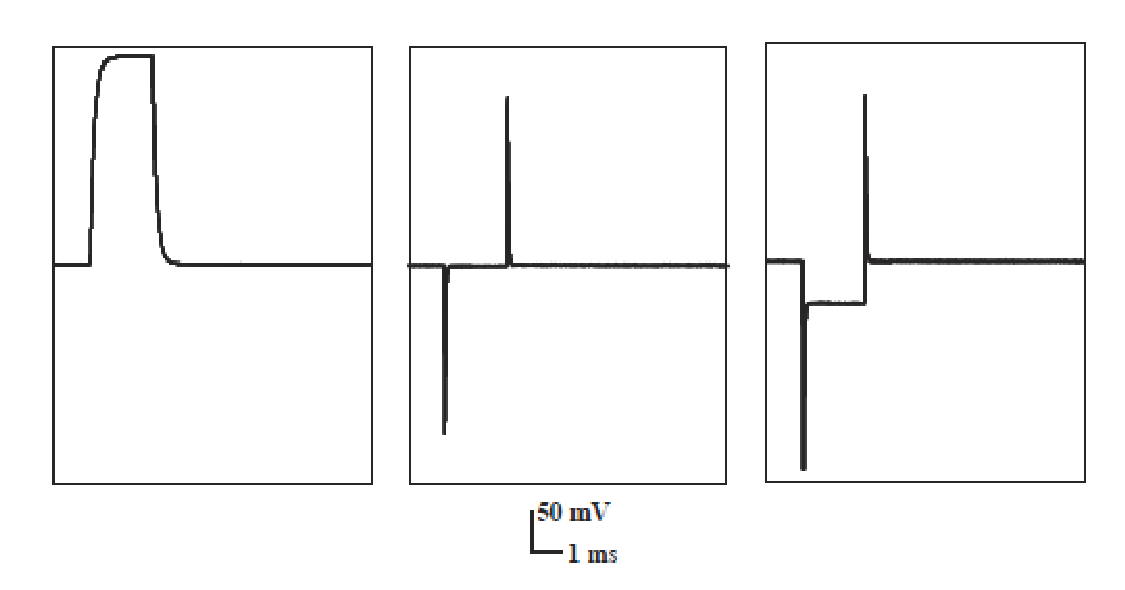
\includegraphics[height=5cm,
    angle=0]{./images/bridge-balance.eps}}
  \caption{(A) no bridge-balance (big voltage drop is recorded at one 2ms
  pulse); (B) optimum bridge balance is used and the voltage drop across the micropipette is eliminated from the record
({\it the transient at the onset and finish of the voltage step is the result
of finite bandwidth of headstage amplifier}). (C) bridge-balance control is
advanced too far [the voltage drop is overcompensated and thus a
reverse-polarity step appears]}
  \label{fig:bridge-balance}
\end{figure}

It is important that the micropipette resistance be constant. Clearly, if the micropipette
resistance varies as the current flows there will be no unique setting of the Bridge Balance
control and the measurement will include an artifact due to the variable voltage drop
across the micropipette.

\textcolor{red}{NOTE}:
\begin{enumerate}
  \item the bridge is an adjustment of the output signal; it has no effect on
  the cell. Operations that not affect the cell is called {\bf cosmetic
  operations}

  \item Operations that affect the cell - which often involve an element of
  positive feedback (Sect.\ref{sec:op-amp_closed-loop_positive-feedback})
  often leads to 'effective' change and is thus not recommended.

  \item A second electrode is often used, to report the 'true' value of
  somatic $V_m$; such electrode is always held with zero current flow (to
  prevent any artifacts would result from voltage drop generated by this
  current)
\end{enumerate}

\subsection{-- Wheatstone bridge}
\label{sec:Wheatstone-bridge}

{\bf Wheatstone bridge} (aka {\it resistance bridge}) is an electric circuit
developped by Samuel Hunter Christie (first described in a paper entitled
"Experimental  Determination of   the   Laws   of   Magneto-Electric Induction"
in  1833). However, Christie's work  also  was  largely  unnoticed, probably
because  his  description  was awkward  and  buried  in  a  long  and somewhat
 tedious    paper.  Charles     Wheatstone     (1802-1875)
referred to Christie's work in a paper in 1843, described it more clearly and
named it {\bf resistance bridge} and  its branches were called 'arms'. The
circuit later beared Wheatstone name.
\url{https://www.ietlabs.com/pdf/GenRad_History/A_History_of_Z_Measurement.pdf}

The circuit {\it measure unknown resistance values} and as a means of
calibrating measuring instruments, voltmeters, ammeters, etc, by the use of a
long resistive slide wire.
Today digital multimeters provide the simplest way to measure a resistance.
Nevertheless, the Wheatstone Bridge can still be used to measure very low values
of resistances down in the milli-Ohms range.
\begin{itemize}
  \item  The Wheatstone Bridge circuit is nothing more than two simple
  series-parallel arrangements of resistances connected between a voltage supply
  terminal and ground producing zero voltage difference between the two parallel
  branches when balanced.
  
  \item  A Wheatstone bridge circuit has two input terminals and two output
  terminals consisting of four resistors configured in a diamond-like
  arrangement as shown.  

STEP 1: two resistors are in series ($R_1$ and $R_2$), the same currents (i)
flow through both of them. Each resistor within the series chain produces an
\verb!I.R! drop, or voltage drop across itself as a consequence of the current
flowing through it as defined by Ohms Law We can see that the source voltage
$V_S$ is divided among the two series resistors in direct proportion to their
resistances.
\begin{equation}
\begin{split}
V_1 &= R_1 \times I \\
V_2 &= R_2 \times I \\
V_S &= V_1 + V_2
\end{split}
\end{equation}
{\it This is the principle of voltage division}, producing what is commonly
called a potential divider circuit or voltage divider network.

STEP 2: In Wheatstone bridge, we add another series resistor circuit,  using the
same resistor values in parallel with the first. As the second series circuit
has the same resistive values of the first, the voltage at point D, which is
also the voltage drop across resistor, R4 will be the same at that in R2, with
respect to zero (battery negative).
But something else equally as important is that the voltage difference between
point C and point D will be zero volts. When this happens, both sides of the
parallel bridge network are said to be {\it balanced} because the voltage at
point C is the same value as the voltage at point D with their difference being
zero.

STEP 3: What if we reversed the position of the two resistors R3 and R4 (or
exchange its values), so $V_{R4}= 0.4 (A) \times 10 (\Omega) = 4$ (Volts).
and D = 4 volts. Then the difference this time is: 8 - 4 = 4 volts..
The voltage difference between points C and D will be 4 volts as: C = 8 volts
The result of swapping the two resistors is that both sides or 'arms' of the
parallel network are different. When
this happens the parallel network is said to be {\it unbalanced} as the voltage
at point C is at a different value to the voltage at point D.  
\end{itemize}
So we can see that a Wheatstone bridge circuit can be used to compare an unknown
resistance $R_X$ with others of a known value, for example, R1 and R2, have
fixed values, and R3 could be variable 
\begin{equation}
\frac{R_1}{R_2} = \frac{R_3}{R_X} 
\end{equation}

\begin{mdframed}

In a DC circuit, only resistors affect current.
The voltage is proportional to the current passing through a resistor based on
Ohm's law: $V=I.R$.


In an AC circuit, there are other quantities  that  affected  current,  at least
 transient  current. They are {\bf capacitors}.
Oliver   Heaviside   (1850-1925)   introduced   the   terms   {\bf impedance Z}
(Sect.\ref{sec:impedance}), "capacitance"  and  "inductance"  in  1892  and  an 
operational  notation  for complex impedances.
Ohm's Law was generalized to $E = I.Z$, where $Z = R + jX$ and  $j=\sqrt{-1}$.
For  a  complex  impedance  the  bridge  balance  equation  now  became
$Z_X/Z_S$ =  $Z_A./Z_B$.

%  - with a resistor R and capacitor C in parallel: an alternating
% current is generated using Wheatstone bridge.
% The alternating current passing through a network with a resistor R and
% capacitor C  in parallel; then the voltage appearing across the network is
% proportional to the current; and the constant of proportionality is called the
% {\bf impedance Z} (Sect.\ref{sec:impedance}).

% The biological membrane is represented as an AC circuit, with 
% \begin{equation}
% V = I . Z
% \end{equation}
If we could measure the impedance Z change during an action potential, then we
can know what change changes in the resistance and capacitance of the membrane.

The value of the unknown resistance $R_x$ can be calculated using  a simple
Wheatstone bridge circuit. 
\end{mdframed}


\begin{figure}[hbt]
  \centerline{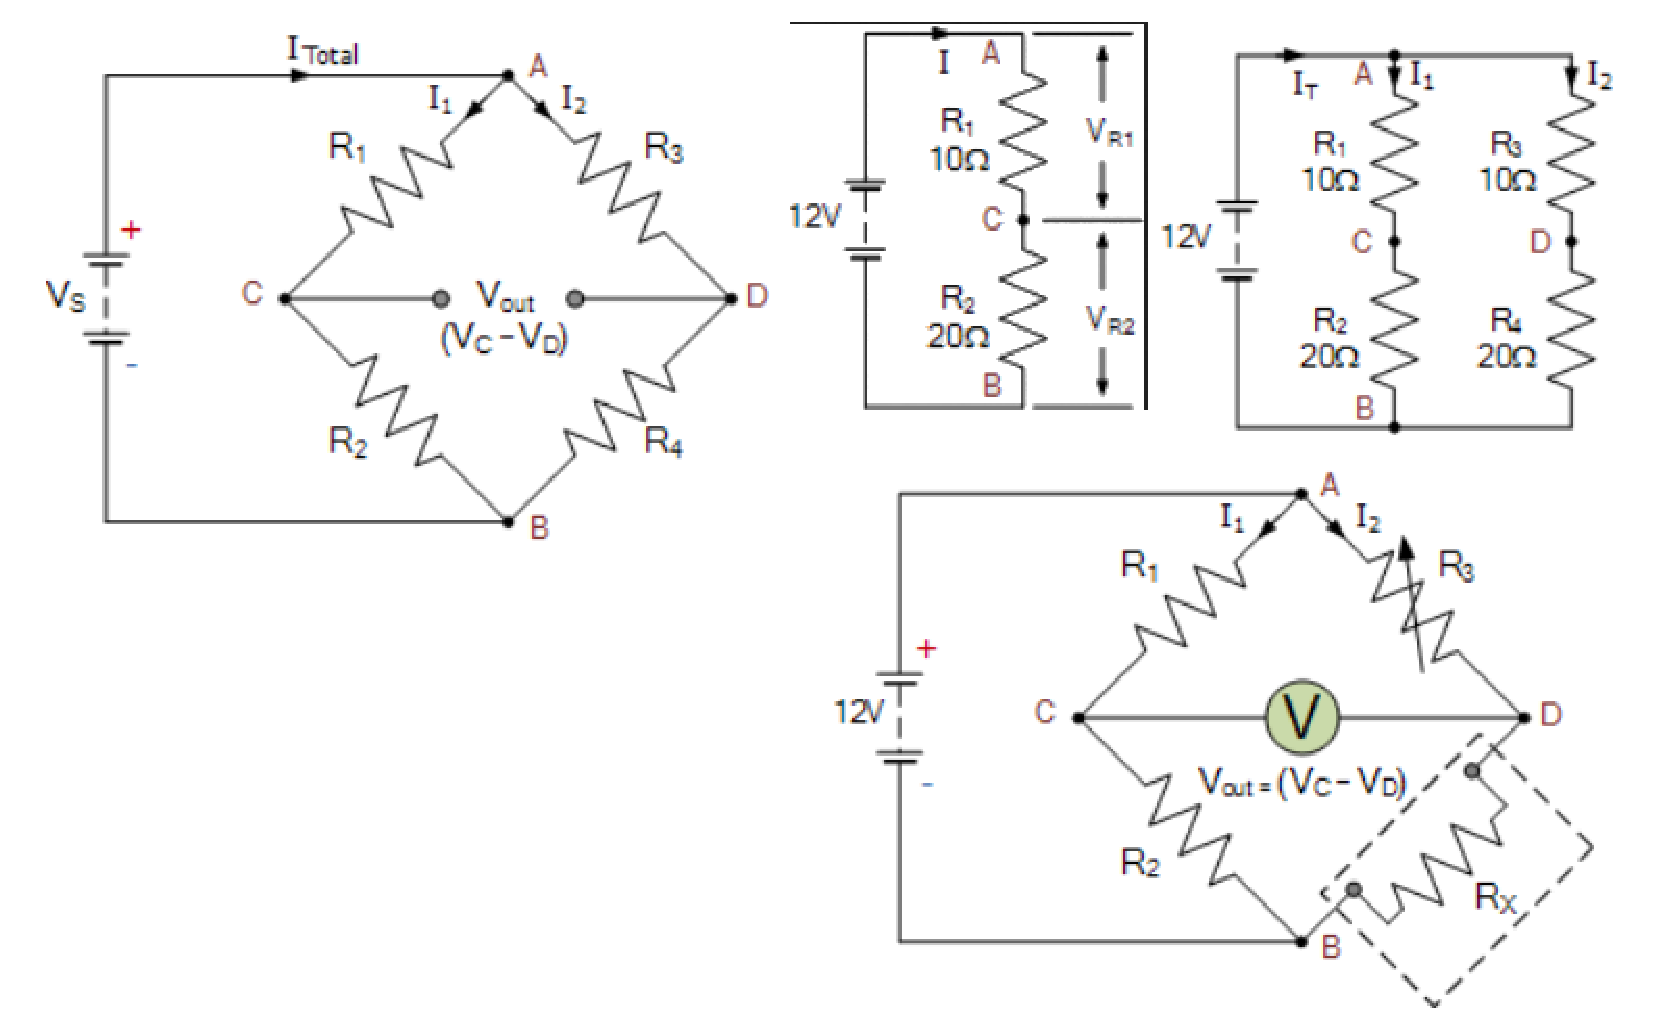
\includegraphics[height=5cm,
    angle=0]{./images/Wheatstone-bridge-2.eps}}
  \centerline{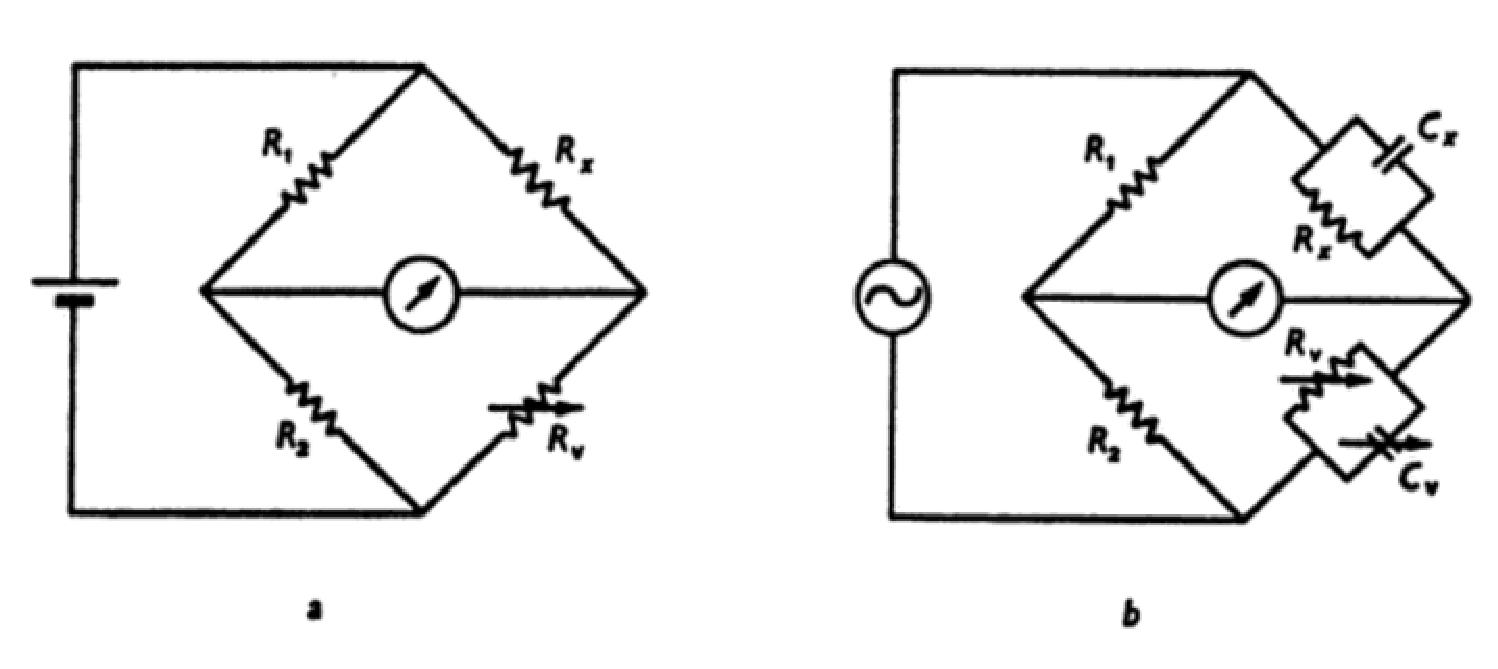
\includegraphics[height=3cm,
    angle=0]{./images/Wheastone-bridge.eps}}
\caption{Wheastone bridge: (A) a simple DC Wheastone bridge to measure
resistance; (B) a simple AC Wheastone bridge to measure resistance $R_x$ and
capacitance $C_x$ in parallel}
\label{fig:Wheastone-bridge}
\end{figure}


\subsection{capacitance neutralization}
\label{sec:capacitance-neutralization}

As shown in Fig.\ref{fig:current-clamp}(C); the output is amplified with a
gain $G$  and then its result is used to charge the parasitic capacitance on the
input.

Assume initially $V_m = V_p = V_\out = 0$ (mV). With a current injection, a step
change in the membrane potential occurs from 0 to new value $V$.



\section{From action potential to voltage clamp}
\label{sec:from-acti-potent}

The understanding of the ionic composition forming an action potential
(Sect.\ref{sec:action-potential}) was not experimentally confirmed until
recording of axonplasm in squid giant axon was made available.

\begin{figure}[hbt]
  \centerline{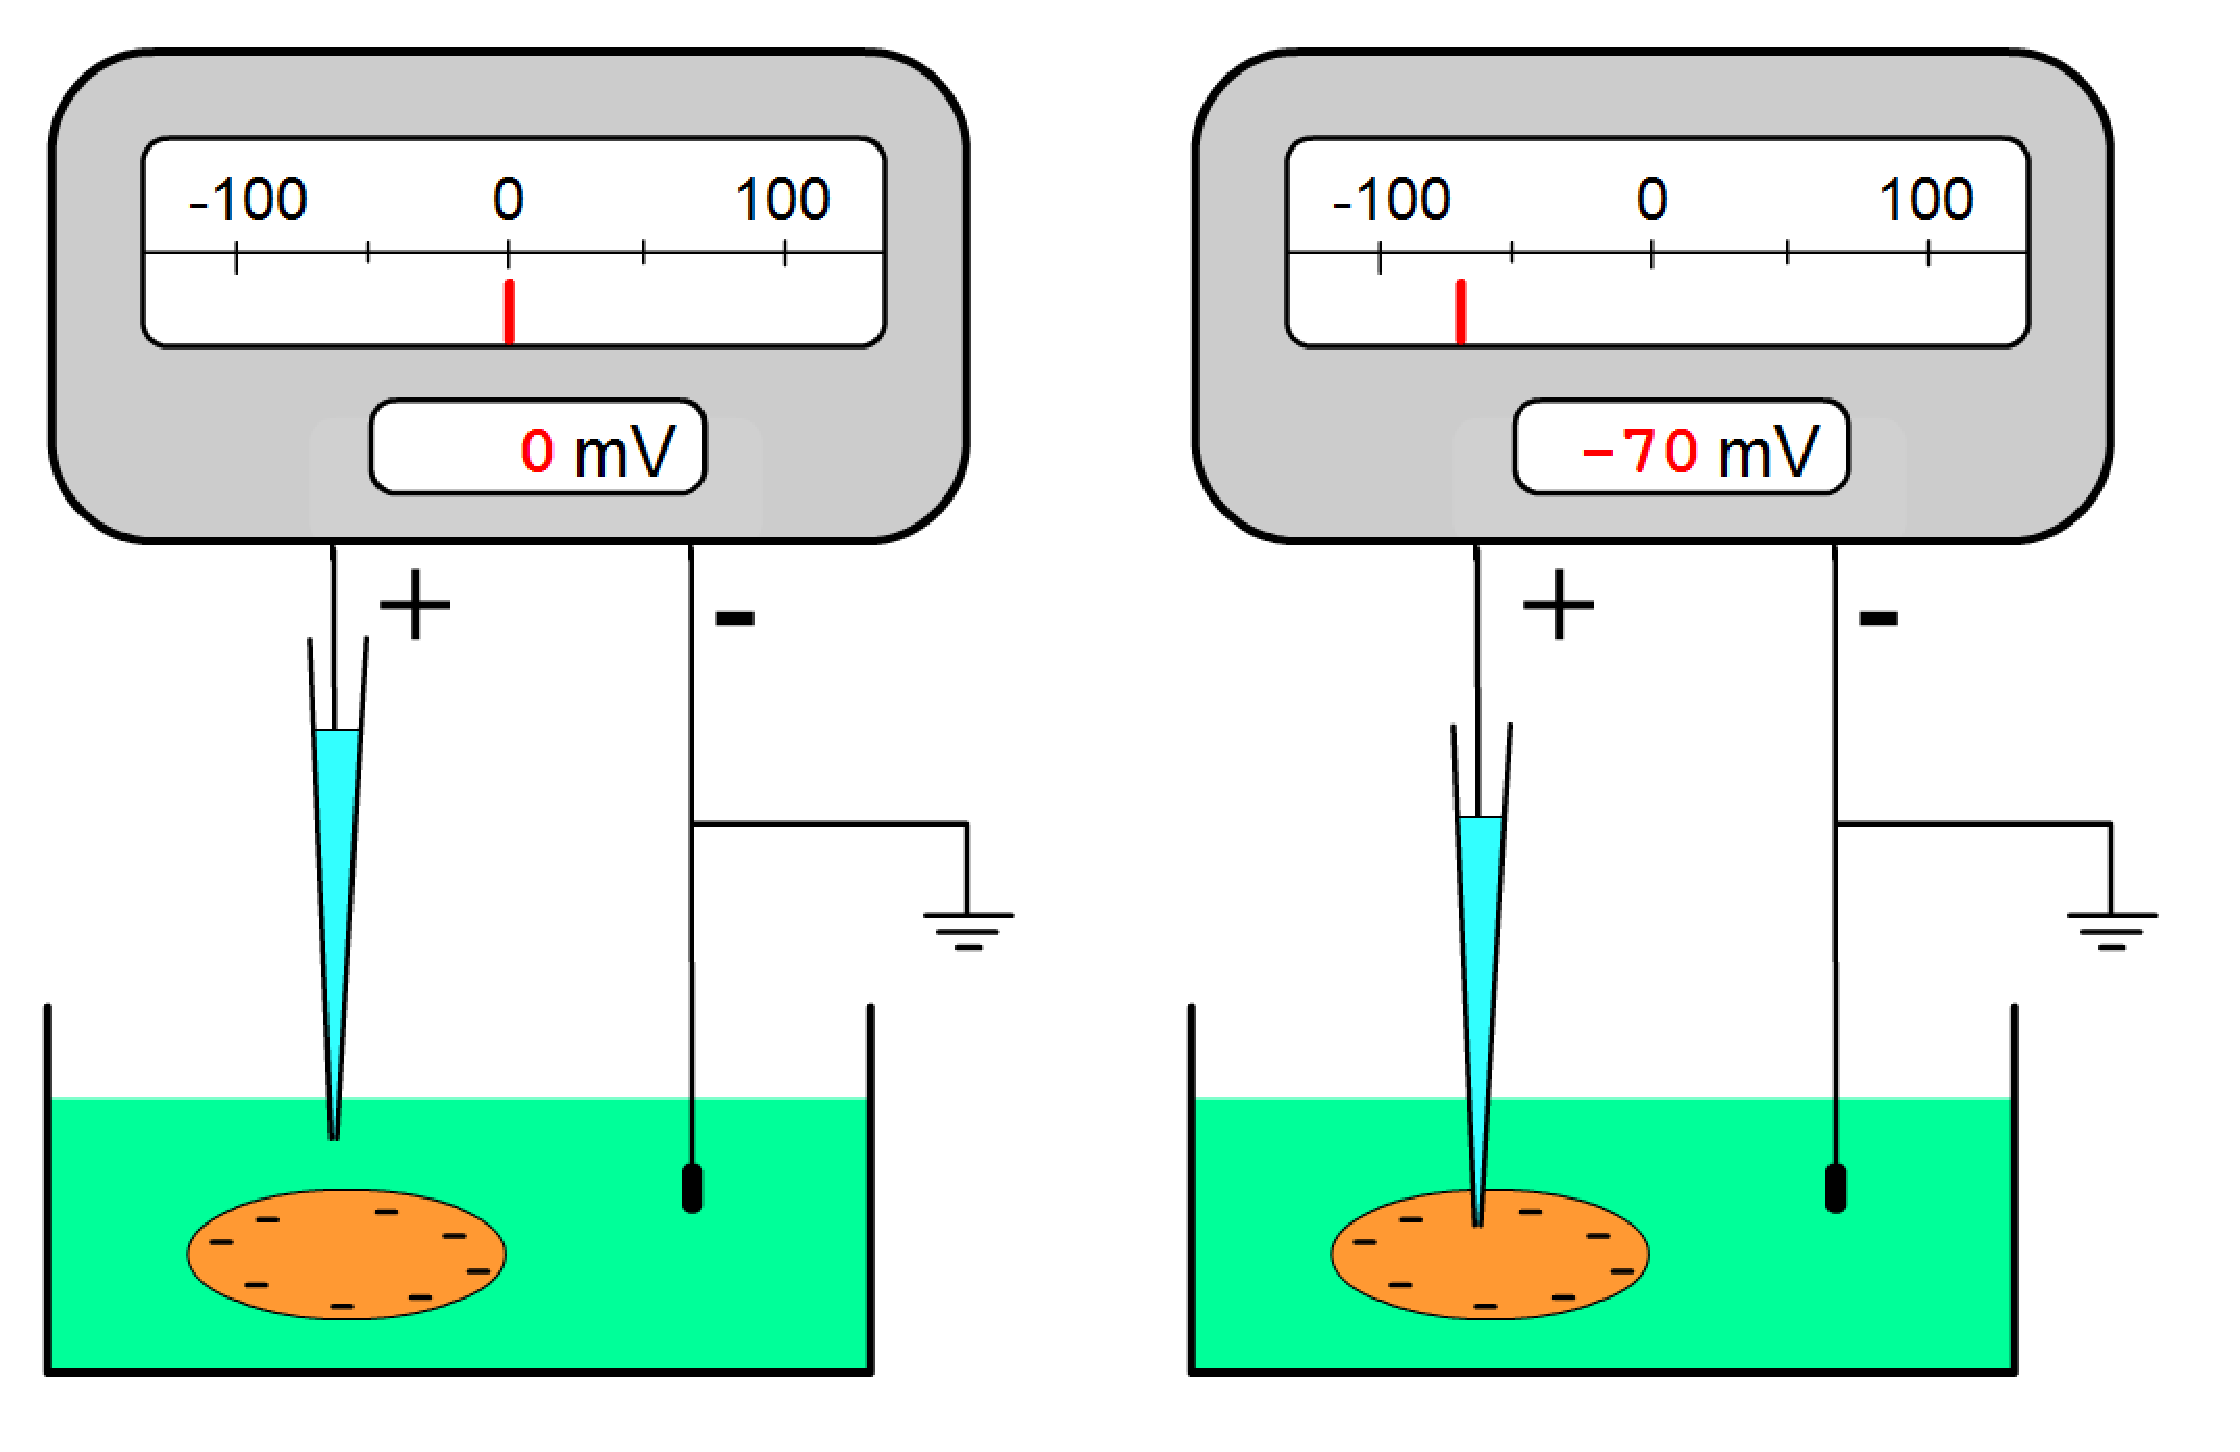
\includegraphics[height=5cm,
    angle=0]{./images/electrode_Vrest.eps}}
  \caption{Detecting resting potential using a microelectrode, which is
  displayed via a specialized oscilloscope or
  voltmeter\footnote{http://www.st-andrews.ac.uk/~wjh/neurotut/mempot.html}}
  \label{fig:microelectrode}
\end{figure}

In an excitable cell (e.g. neuron, myocyte), the change in ionic conductance is
a function of both voltage, and time. Also, the change in membrane potential
affects the gating of ion channels which provides a feedback loop back to the
membrane potential. This loop of interaction make it very hard to measure the
ionic conductance. We need a way to fix one variable, e.g. voltage, to be able
to measure the current over time.

In 1912, Hober first used high frequency impedance measurement
(Sect.\ref{sec:electrical-impedance-method}) on biological materials - measure
the conductivity of a suspension of erythrocytes.

Fricke first suggest an equivalent circuit for living cell; and developed the
theory of electrical impedance measurement.

In 1939, Cole and Curtis (\citep{cole1939}) extended the measuremet, used a
Wheaston bridge (Sect.\ref{sec:Wheatstone-bridge}) with high alternating
current (2 to 1000 kHz) to measure the transient increase in membrane
conductance during AP to marine eggs, muscle, nerve and various other tissues.
\begin{itemize}
  \item determine change in electrical properties of {\it Nitella}; the squid
  giant axon during activity

They suggested that electrical impedance measurements of muscle might throw
light upon the membrane changes which accompany the action of certain agents,
especially narcotics.
  
  \item the membrane capacitance $C_x$ was showed to be around 1.1 $\muF/\cm^2$
  (in resting condition) - as shown in the oscilloscope with thin line (i.e. no
  broadened range); and felt about 2\% during activity.
  
  \item the resistance $R_x$ however fell very remarkedly during activity; from
  1000 $\Omega$.cm$^2$ (resting condition) down to 25 $\Omega$.cm$^2$ (during
  activity).
\end{itemize}
The electrical circuit for the biomembrane is then generated with two additional
components: axial resistance (longitudinal resistance) of the external medium
$r_o$ and longitudinal resistance of the axoplasm $r_i$ and is called {\bf
core-conductor theory} (Sect.\ref{sec:core-conductor-membrane}).



\section{2. (Whole-cell) intracellular recordings (record voltage mV, current
nA)}
\label{sec:intracellular-recording}
%\section{Voltage-clamp technique}
\label{sec:voltage-clamp-techniques}
%\section{Voltage Clamp}
%\label{sec:voltage-clamp-techniques}

Whole-cell recordings integrate the response of a large number of potentially
heterogeneous ion channels. Isolating these ionic current components is a
critical step (Sect.\ref{sec:isolating-ionic-current-components}).

As the membrane is formed by a resistor $R_x$ and capacitor $C_x$; the idea is
to hold the voltage constant to study the conductance through the membrane.

In 1939, Hodgkin, Huxley and Cole made the first squid giant intra-axonal
recordings. The voltage will be measured at the tips of the electrode.  However,
as the ``clamp'' on voltage decreases fairly quickly (along the axon), the clamp
cannot keep the voltage steady and uniformly.

In 1949, to break the feedback loop, a technique developed by Marmont (and Cole
used that for his experiment), known as {\bf space clamp} is used to hold the
voltage $V_m$ at a level of interest, i.e. isopotentiality over a region of axon
by threading a wire along the interior of the axon to short-circuit the
longitudinal resistance of the axoplasm - Sect.\ref{sec:space-clamp}. This was
later adopted by Hodgkin-Huxley to developed their landmark model
(Sect.\ref{sec:voltage-clamp-hodgkin-huxley}.



In 1982, Sakmann and Neher developed {\bf patch-clamp} (``Giga-seal'') that
allow the determination of a single ion channel kinetics\cite{fishmann1975pvc}.


Whole-cell recording~\cite{kay1986ans},\cite{numann1987ocs}.
The basic idea is to insert a conductive medium (the electrolyte filling the
pipette, e.g. 1-3 M KCl) through the cell membrane with minimal damage to the
cell, Fig.\ref{fig:Ling-Gerard-3-electrodes}. The quality of electrodes is very
important (Sect.\ref{sec:electrode}).


  \begin{figure}[htb]
    \centerline{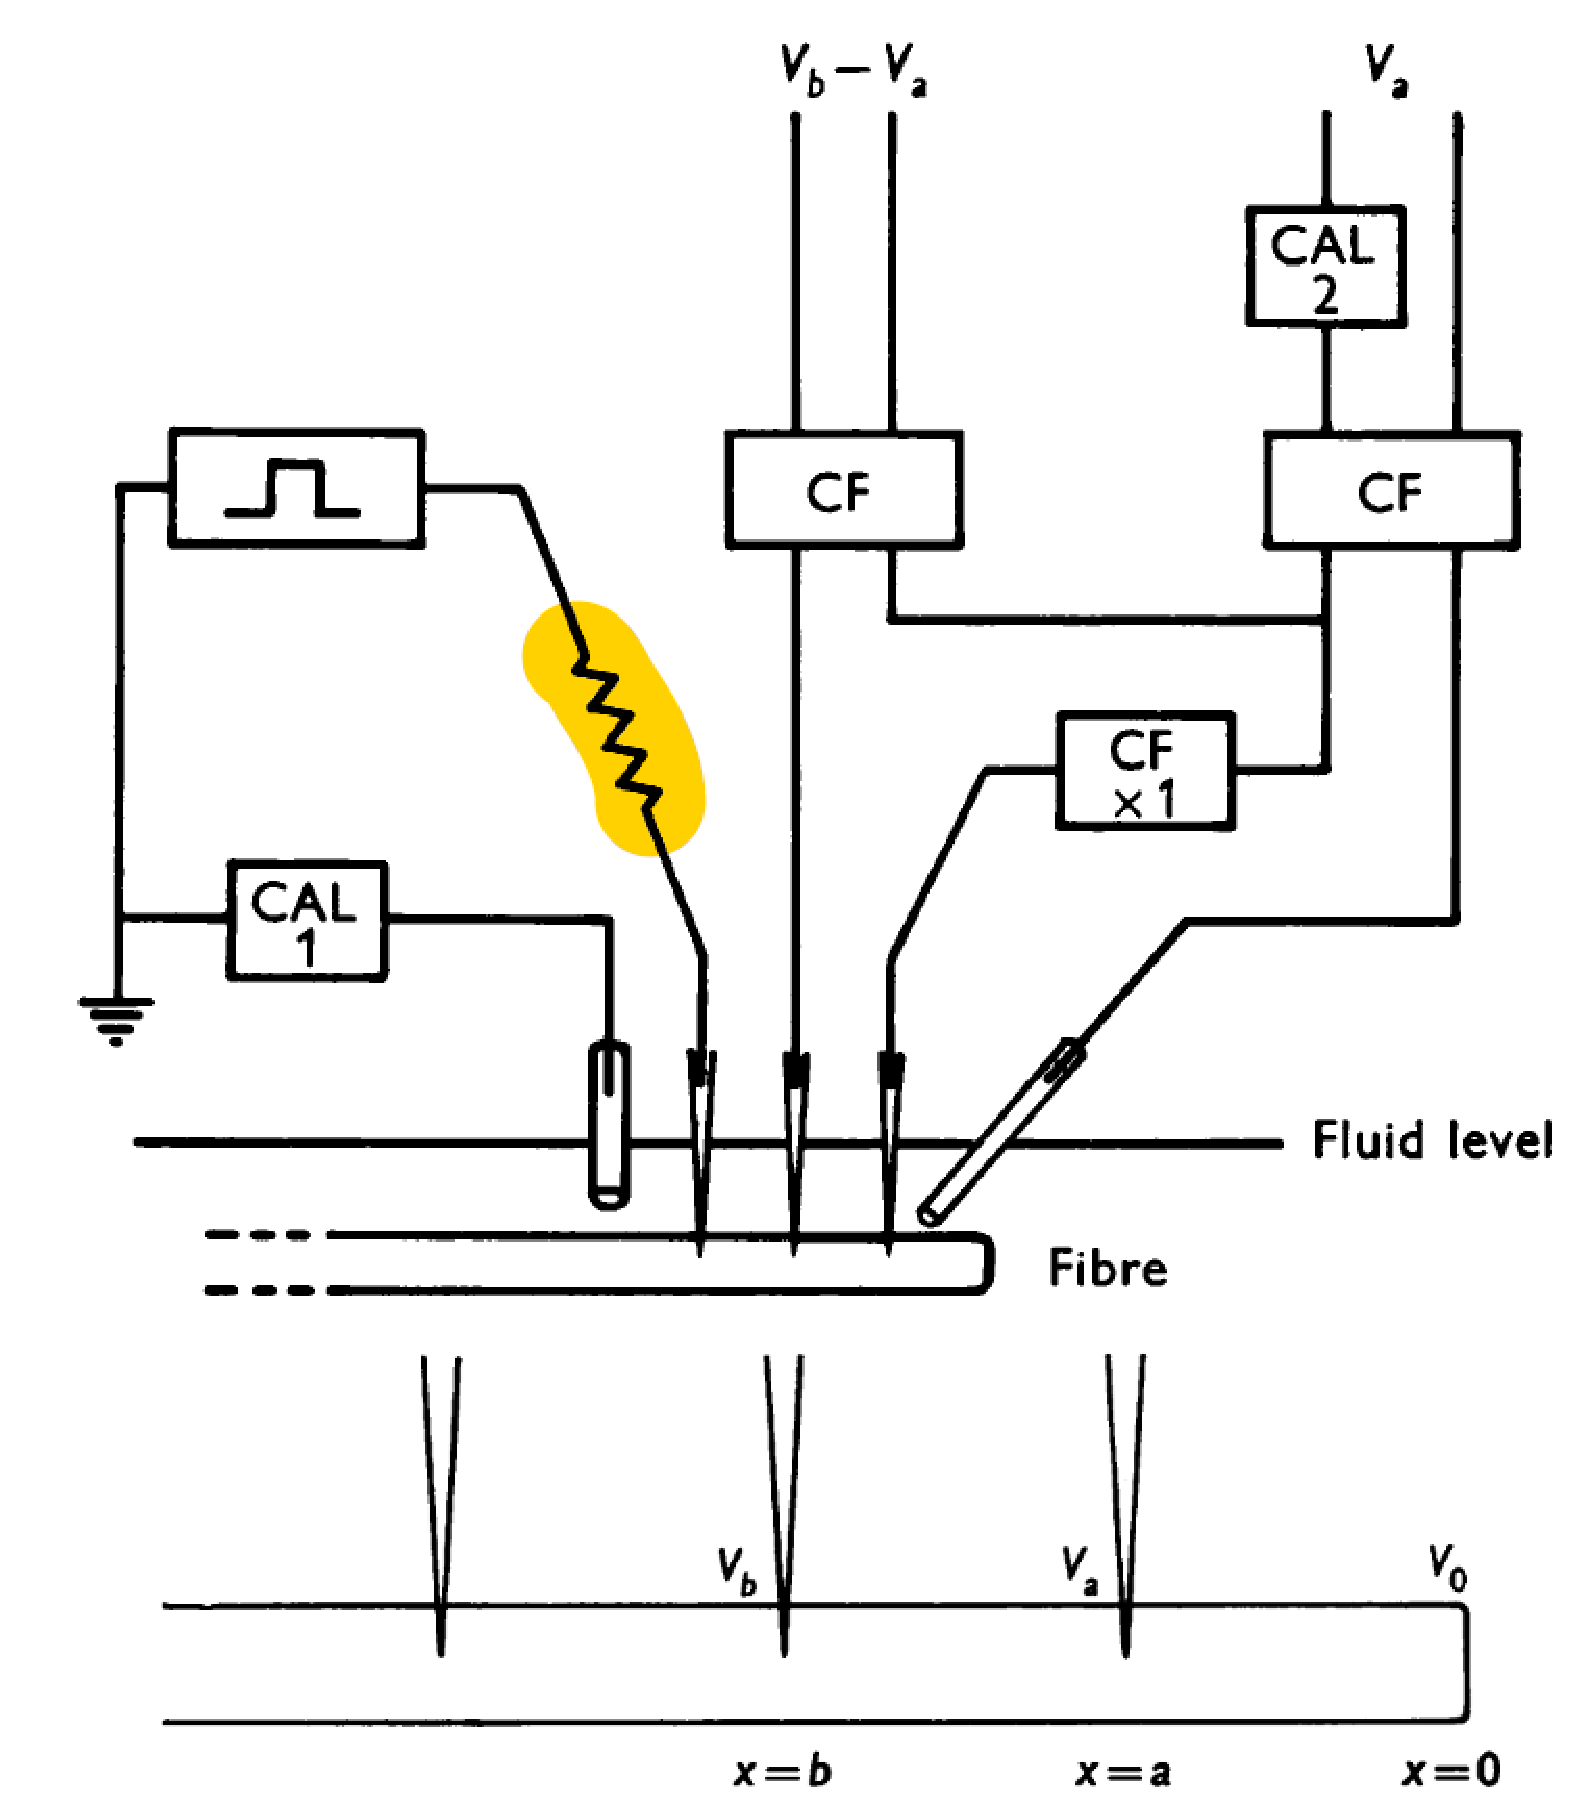
\includegraphics[height=5cm]{./images/Ling-Gerard-3-electrodes.eps}}
    \caption{Recording apparatus using 3 micro-electrodes of Ling-Gerard type
    (Adrian, Freygang (1962)) }\label{fig:Ling-Gerard-3-electrodes}
  \end{figure}

Using squid giant axon, the axons were mounted in an air-gap chamber (Fishman,
1970). The ionic concentrations on both side of the membrane were kept under
close control; and the current across the membrane of the central 3mm of axon
was measured, with 20mm length clamped by means of 3-plate guard-electrode
system (Moore, Cole, 1963). In Fig.\ref{fig:Ling-Gerard-3-electrodes}, the fiber
is sartorious muscles of English frogs ({\it Rana temporaria}). The sartorius
was left attached to the split pelvic bone; with all other muscles removed to
espose the ends of the fibers at their attachment to the pelvic tendon (see
Adrian, Freygang (1962)).
\begin{enumerate}
  \item the micro-electrodes are 445 $\mum$ apart - and one of them is $445\mum$
  from the end of the fiber.

  \item the electrode is in series with either a 100 M$\Omega$ or 1000 M$\Omega$
  resistor. Also, the resistance of the electrode itself is between 5 to 20
  M$\Omega$; with the tip potentials less than 5 mV.

  \item the electrodes are filled with 3.0 M KCl.

  \item among the three electrodes: two are used for recording potential
  at two locations (first and second ones). NOTE: the third one is the one
  nearest to the end of the fiber.

  \item an amplifier Tektronix 502 (double-beam oscilloscope) is used for
  displaying transmembrane potential: between the one nearest to the far end of
  the fiber and the external fluid.

  \item an amplifier Tektronix 502 (double-beam oscilloscope) is used for
  recording the different in potential at micro-electrodes 1 and 2.

  \item the fiber is putt in a large volume of conducting fluid, assuming
  potential of the outer surface of the membrane w.r.t. the distant point can be
  considered as zero.

  \item current is inserted at the 1st (left-hand) electrode and alter the
  membrane potential by $V_a$ at $x=a$ and by $V_b$ at $x=b$.

  \item \textcolor{red}{experimentally, we can measure $V_a$ and $(V_b - V_a)$}.

\end{enumerate}

As the gating of ion channel is a function of voltage (or transmembrane
potential), it is important to control this membrane potential (at different
value) to see (1) steady-state behavior and (2) the dynamics of the change from
one steady-state (equilirbium) to a new equilibrium.

The principle of voltage clamp technique was developed by Marmont and Cole
(1949) for the squid giant axon; whose method was applied by Hodgkin and Huxley
to idenfity different ionic components regulating the transmembrane potential
(Vm) and then developed the first mathematical model representing the dynamics
of such transmembrane potential (Vm). Details is covered in
Sect.\ref{sec:from-acti-potent}. Also, to study the gating of ion channels,
different protocols have been utilized - voltage-clamp protocol
(Sect.\ref{sec:voltage-clamp-protocol}).

\textcolor{red}{APPROACHES}
\begin{enumerate}
  \item  Micropipette voltage-clamp techniques for whole-cell current measurement traditionally
assign the role of potential measurement and current passing to two different intracellular
micropipettes.

Early approaches use 2 electrodes: one to measure the voltage, and one to pass
the required current Ip  to ensure that the voltage recorded remains constant
whatever currents flow in the cell. By knowing the holding voltage, and the
injected current Ip; the current through the ion channel can be measured.
However, it is often impractical or impossible to use two electrodes.
So, typically a single electrode is used.

  \item 
\end{enumerate}





\subsection{Space-clamp (Marmont's clamp, 1949)}
\label{sec:space-clamp}
\label{sec:Marmont-clamp-device}

Space-clamp refer to the effort to clamp the voltage across a region (in space)
along the axon. NOTE: In a full neuron, due to the wide spreading in space,
ensuring the uniform of transmembrane voltage everywhere is a challenging
task. This is known as {\it space-clamp problem} when doing whole-cell
voltage-clamp (Read Sect.\ref{sec:space-clamp-problem} to understand better
about space-clamp problem.)

To keep the membrane potential uniform along a region/segment of axon, it means
that we need to prevent the axial current, i.e. longitudinal current along the
axon fiber.

\textcolor{red}{The question is how to prevent {\it axial current}?}
In 1949, a technique developed by Marmont (and then used by Cole to do the
voltage-clamp experiments), known as {\bf space clamp} is used to hold the
voltage $V_m$ at a level of interest, i.e. isopotentiality over a region of
axon (described in details in Sect.\ref{sec:space-clamp-axon}.

Cole's later used that device to perform a number of voltage-clamp experiments
(Sect.\ref{sec:voltage-clamp-Cole-Marmont}).



\subsection{-- in the axon: 2 electrodes (lateral guard electrode + 1
axial-wired internal electrode) + electronic-feedback circuit}
\label{sec:space-clamp-axon}

In the 1930's, the huge axon of the squid become a favorite tool to study the
basis of action potential. It is important to study transmembrane current $I_m$
(Sect.\ref{sec:transmembrane-current}) at a short-enough segment over time.
This requires 2 things: (1) keep the membrane potential constant, (2) no axial
current (so that the current measured is the transmembrane current).

In neurons, with a long axon or dendrite tree, the current can flow in two
directions: the transmembrane potential, and the
presence of axial currents $I_\axial$.

In summer 1947,  George Marmont (while working with Kacy Cole) developed a
technological breakthrough to 'block' the axial current. 
Marmont used two electrodes and an electronic feedback circuit to help fixing
the transmembrane potential $\Vm$. His two electrodes consisted of fine wires
twisted (i.e. in a double spiral) around an insulating glass rod,  which
provides support and prevents the wires from touching each other.
This was before the era of micro-electrodes (Sect.\ref{sec:micro-electrodes});
and thus could be only used on large cells.

% achieve isopotentiality over a region of axon.
\begin{enumerate}
  \item   One electrode (axial wire) with {\it very low resistance per unit
  length} is inserted into the axon, which is bathed in a volume of high
  conductivity, e.g. sea-water. 
  This single electrode is used to measured the internal voltage and,
  simultaneously, to pass the current.

The key to this technological {\it tour de force} was to add chloride carefully
to the silver axial wire (along the interior of the axon), thereby reducing the
surface resistance and junction potential that would normally act as barriers to
current flow in the wire.
This helps to short-circuit the longitudinal resistance of the axoplasm,
Fig.\ref{fig:space-clamp-axon}.
This technique resulted in a uniform potential throughout the length of axon
surrounding the wire, {\it eliminating longitudinal voltage gradients and thus
eliminating propagation}. This helps them to measure the transmembrane current
$I_m$ more accurately.

Marmont was also able to restrict transmembrane current measurement to a short
central segment of the axon membrane (now with uniform potential).  Thus the
radial membrane current, i.e. transmembrane current $I_m$, measured in the
central region of the axial wire was not contaminated by any longitudinal (or
axial) current.

  \item One external electrode (lateral guard electrode, and is a spiral
  electrode),  for current and potential measurement.
\end{enumerate}

The mathematical form of this transmembrane current is given in
Sect.\ref{sec:cable_equation}

\begin{itemize}
  \item The external resistance is very low because of the large volume of
  solution in which the axon is immersed

  \item The internal resistance is made virtually zero by the insertion of the
  metal wires that short-circuit the resistance of the cytoplasm inside the
  axon. This make the inside of the length of axon with wired having a uniform
  voltage, i.e. no longitudinal current (i.e. no sag in membrane potential to
  occur).
\end{itemize}


\begin{figure}[hbt]
  \centerline{
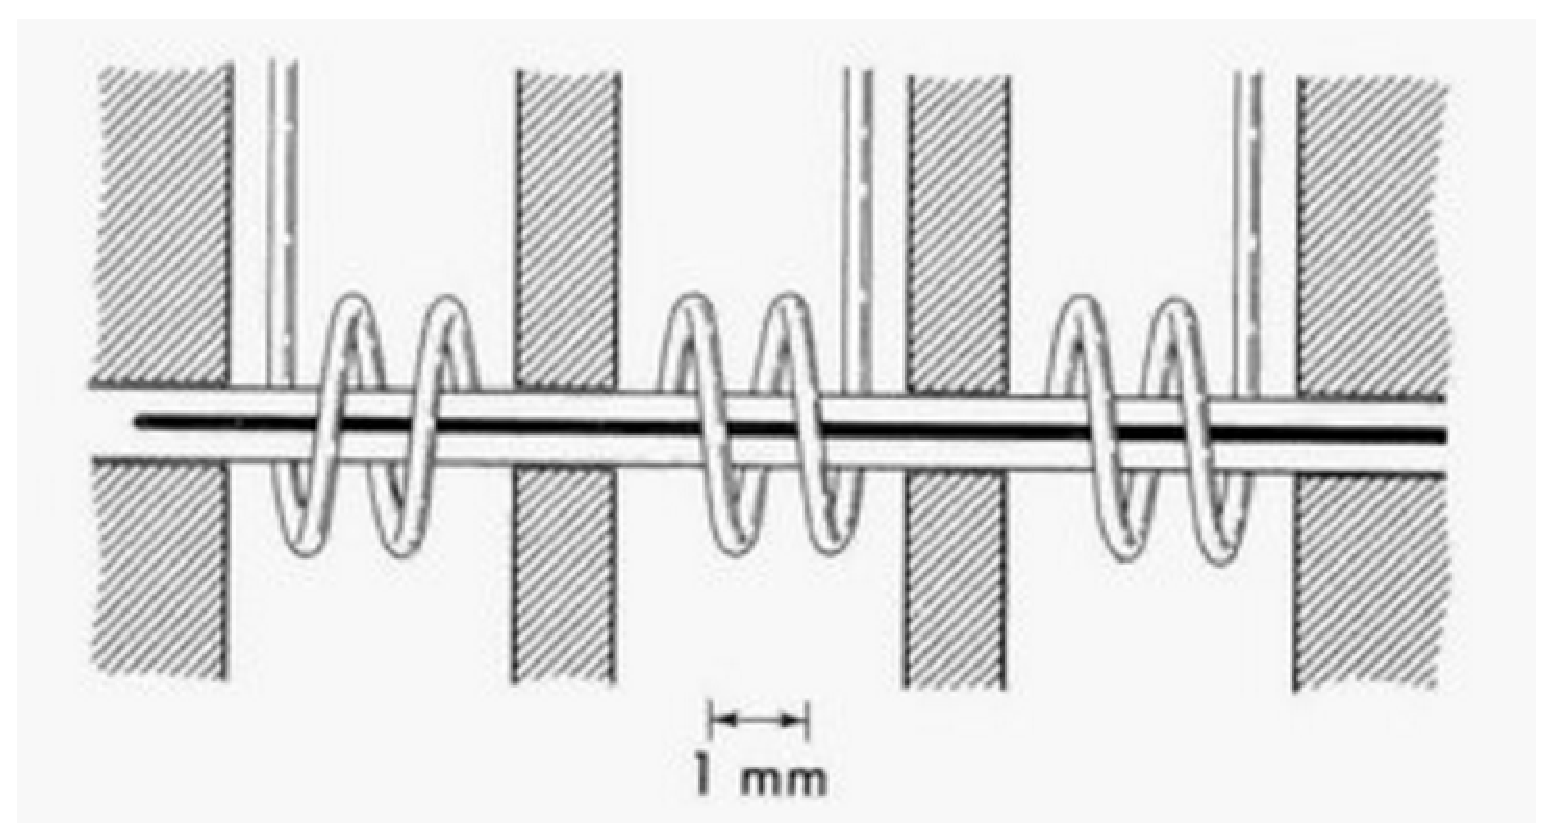
\includegraphics[height=4cm,
    angle=0]{./images/space-clamp-axon.eps}
    }
\caption{Marmont's space clamp with lateral guard electrodes: the squid axon
passed through the holes in the shaded insulating partitions. The central
outside spiral electrode, for current and potential measurement, was between
similar guard electrodes. The internal electrode, solid line, was inserted from
the right to lie in the center of the axon to short-circuit the longitudinal
reistance of the axoplasm}
\label{fig:space-clamp-axon}
\end{figure}



\begin{figure}[htbp]
\centerline{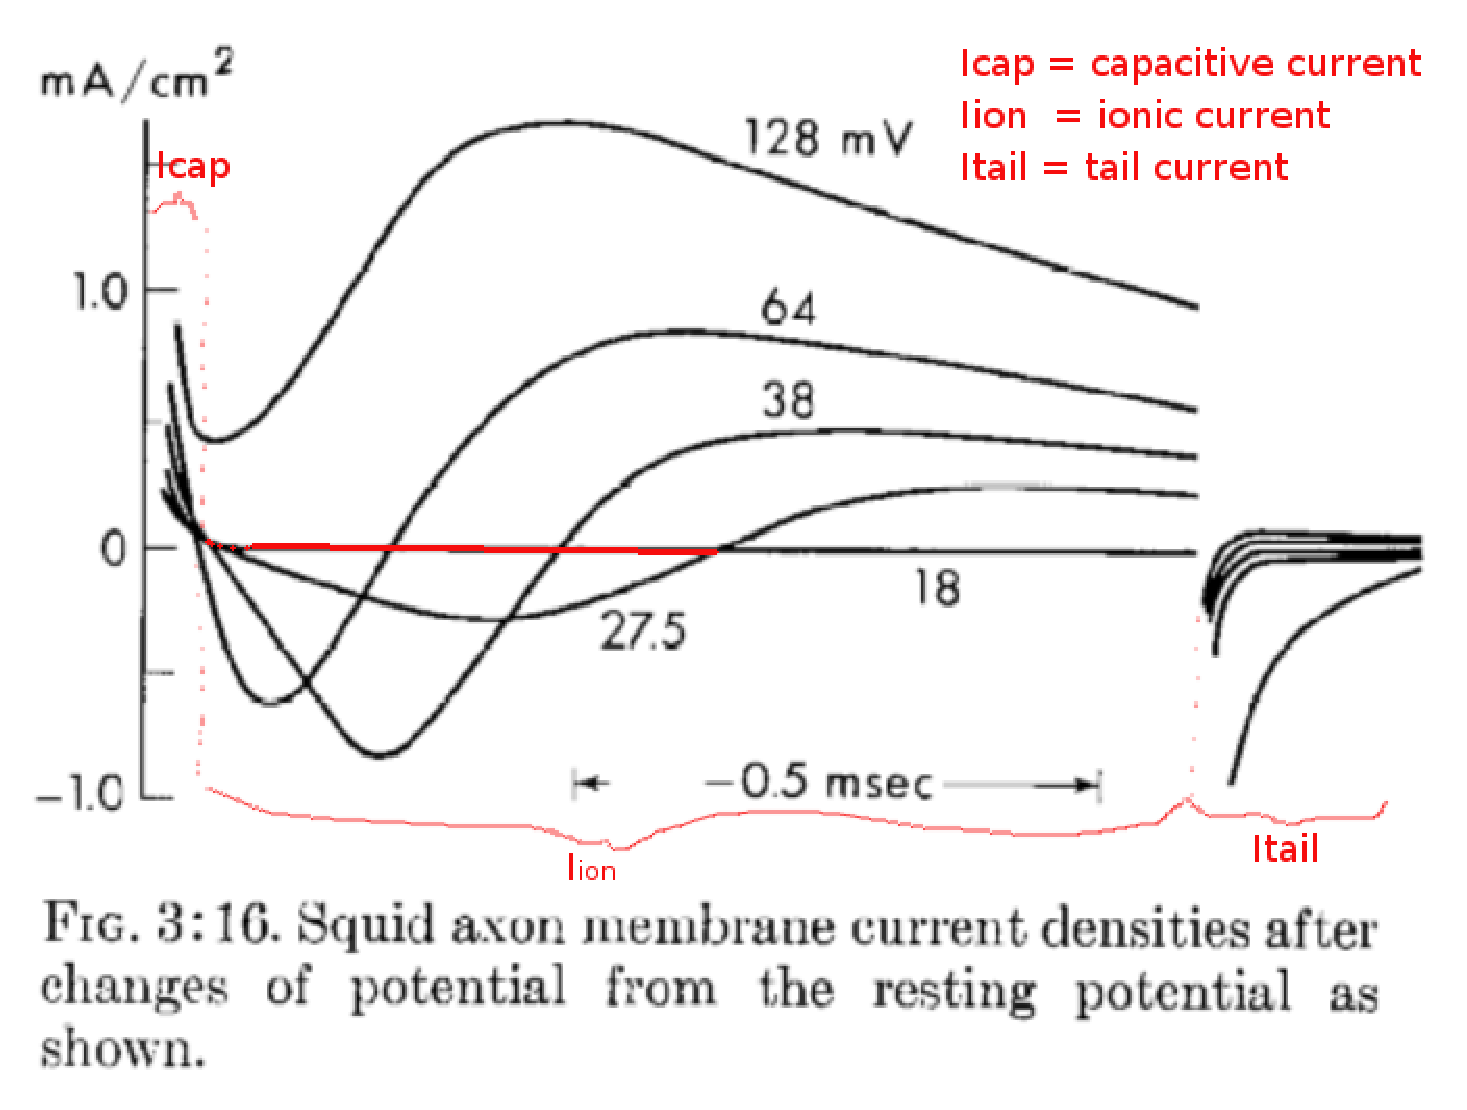
\includegraphics[height=6cm]{./images/voltage-clamp-Cole.eps}}
\caption{Different traces of the current density (mA/cm$^2$) recorded across the
membrane at different voltage clamp by Cole. The value of each voltage step is
indicated next to the current record that it produced}
\label{fig:Vm-clamp-Cole}
\end{figure}

\subsection{-- (Cole's (voltage) clamp)}
\label{sec:voltage-clamp-Cole-Marmont}

Kenneth S. (Kacy) Cole shared a lab at the Marine Biological Laboratory in Woods
Hole, MA, with Marmont. Cole used the device developed by Marmont
(Sect.\ref{sec:space-clamp-axon}) to perform his own experiment with different
conditioning step potentials ($V_c$: command potential).

Initially, the transmembrane potential of the axon was at a holding potential
which is resting potential ($\Vm=V_\rest$) in this case. Also, the command
potential $V_c$ is also at this value.

Now, we want to clamp to a new value. Then, the command potential is given a
series of depolarizing voltage steps away from rest: starting from t=0, and hold
the voltage step for 1ms, Fig.\ref{fig:Vm-clamp-Cole}. The electronic feedback
circuit provide a third current $I_p$ (or $I_\inj$) generated by the difference
in $V_c-V_m$.
\begin{equation}
I_p = \frac{V_c - V_m}{R_m}
\end{equation}
with $R_m$ is membrane resistance.

\textcolor{red}{The most interesting feature of the voltage-clamp data is that
when $V_c$ is set to a value above the resting potential, a brief net inward
current is generated followed by a long-lasting net outward current}.


This current $I_p$ is injected into the intracellular media via a second
injected electrode, with the goal is to change $V_m$ to a new value $V_c$. This
change is not instanteneously, but has a short delay; during which a capacitive
current is generated. In overall, there are two intrinsic currents across a
membrane: capactive current $I_\cap$ (Sect.\ref{sec:capacitive-current}) and
ionic current $I_\ion$ (Sect.\ref{sec:ionic-currents}).

\begin{itemize}
  \item During the time  $V_m$ jumps from the holding potential to a new value
  $V_c$, it causes a capacitive current (Sect.\ref{sec:capacitive-current}):

  NOTE: A capacitive current appears only at
  the beginning of the step, i.e. during $dV/dt>0$.
  \begin{enumerate}
    \item positive: when $\Vm$ jump from resting value to a larger step value
    \item negative: when $\Vm$ jumps from a step value to a smaller resting
    value
  \end{enumerate}

Once $\Vm$ is established to the new value $V_c$, the capacitive current
disappear, i.e. $I_\cap = 0$. So, we can isolate the capacitive current from the
ionic current, by ignoring the current at a short time period after the voltage
change.
% the first and last short time of clamping the $\Vm$ for a certain period.

  \item Once $\Vm$ is set to a new value $V_c$, if $V_c$ is depolarized
  enough, it also triggers the opening of ion channels $I_\ion$.

  During the clamping time, the ionic current $I_\ion$ change smoothly (but not
  instantaneously, regardless of the voltage step being used).
%   So, it's not
%   all-or-none behavior.

  \begin{enumerate}

    \item an early stage: net inward ionic current (after a short delay due to
    capactivie current) starting to see at $V_\step=+18$ mV, \textcolor{red}{red part,
    negative part}) increase downward smoothly (i.e. peak is more negative),
    until reaching a peak value - {\it lasting about 1.5 msec}).

    At different value of voltage clamp, the inward current bends at different
    angle, and reaching different peak values.
    The peaks of these  inward current reaches the 'max' value at $V_\step$ =
    +38 mV), and then decrease in amplitude (i.e. the peak is less negative, as
    shown in trace $V_\step=+64$mV).

    We no longer see this inward current between trace $V_\step$ = +64 mV to
    +128mV.

    \item a more slowly developed outward current follows the inward current.

    The amplitude (i.e. the peak) of the outward current also dependent on the
    level of depolarization. However, in constrast to the inward current, the
    direction of the flow of this later current doesn't reverse.

  \end{enumerate}

  \item During the time  $V_m$ jumps from the clamped potential
  $V_c$ to the resting potential, it causes a tail current
  (Sect.\ref{sec:tail_current}):
\end{itemize}


The drawback of Cole's data is the delayed onset of the sag (i.e. decline) in
membrane potential, rather staying at a steady value (Check Hodgkin-Huxley's
better protocol).  Cole's voltage clamp used a single axial wire to measure the
internal voltage and, simultaneously, to pass the current. Thus, when Cole
showed Hodgkin and Huxley his voltage clamp data, they conjectured that
electrode polarization might have caused the sag in the sustained outward
current in Cole's records.

Cole showed his results to Alan Hodgkin and Andrew Huxley, suggesting the
possibility that the outward current was related to potassium but gave no
explanation for the inward current. Hodgkin and Huxley then performed their own
experiments and developed the mathematical theory of the observation which
brought them the Nobel prize later
(Sect.\ref{sec:voltage-clamp-hodgkin-huxley}).
\footnote{\url{http://fohs.bgu.ac.il/nia/NIA2003/neurolab/appendix/local.ref/kacvclmp.htm}}

% Also, the possibility that this early inward current might be
% carried by Na ions fit with Hodgkin, Huxley, and Katz's observations that the
% overshoot of the action potential was dependent on the external Na
% concentration.

Marmont and Cole were able to study what has come to be called
membrane {\bf action potentials}. He stimulated the membrane patch with square
pulses of current and carried out numerous experiments to see how changes in
ions and the introduction of drugs altered the action potential shape.
\textcolor{red}{Despite his important advance, Marmont was unable to determine
the basis of the generation of the impulse from his experiments} - which was
later discovered by Hodgkin-Huxley.

We will discuss how this was tackled in the axon recording
(Sect.\ref{sec:space-clamp-axon}) and soma recording
(Sect.\ref{sec:space-clamp-soma}).


% \subsection{-- Cole's clamp}
%
% % The change in $\Vm$ affects the gating of the channel (e.g. making the channel
% % in conducting state), and in turns, the opening of the channel enable the movement of ions
% % that cause the change in ionic concentration gradient which provides a negative
% % feedback to the $\Vm$.
%
% In an excitable cell (e.g. neuron, myocyte), the change in ionic conductance is
% a function of both voltage, and time. Also, the change in membrane potential
% affects the gating of ion channels which provides a feedback loop back to the
% membrane potential. This loop of interaction make it very hard to measure the
% ionic conductance. We need a way to fix one variable, e.g. voltage, to be able
% to measure the current over time.

\subsection{-- in soma}
\label{sec:space-clamp-soma}

This part is not present, as the original epxerience focused on long
axon. (Probably, the soma is considered a spherical shell so clamp the soma
only).

\subsection{-- space-clamp problem}
\label{sec:space-clamp-problem}

Also, {\bf space-clamp problem} refers to the challenge when
trying to achive the uniform potential for the neuron which typically have
very large morphology.

It means the technique try to clamp the voltage equally along the length of the
axon or dendrite or across neuron (if the electrode is plugged into the somata)
yet due to the very long structure of morphology, the voltage is not completely
uniform everywhere. As such, the recorded current is not the transmembrane
current (via opening ion channels); but also include the axial current
$I_m=I_\ion - I_\axial$.

When you're trying to estimate the current via sodium channel, if sodium
conductance density is too high; it may reduce the effect of space clamp, i.e.
the compensated injected current does not have enough time to diffuse compare to
high inward flux to keep membrane potential at all locations the same.

To improve space clamp conditions, it was necessary to reduce sodium currents in
most experiments by adding low concentrations of tetrodotoxin (TTX, 40 nM)
(Huguenard et al., 1988; Reckziegel et al., 1998). NOTE: Properties of native
and TTX-reduced currents were not different (cf. Reckziegel et al., 1998)

As there are many things to take into account during the experiment, the early
voltage-clamp technique is applicable only to spherical cells (or cells with
small size) whose membrane potentials can be assumed the same everywhere.

As the 'clamp' voltage is indeed the voltage measured at the tip of the
voltage-clamp electrode. In nonspherical cells, such as neurons, the membrane
potential at regions far away from the tip of the voltage-clamp electrode is not
clamped properly. This means that the current recorded by the voltage-clamp
electrode is the sum of the {\it local current across the membrane} and {\it of
axial currents} from locations experiencing different membrane potentials.

\subsection{Hodgkin-Huxley's clamp (1950): 2 electrodes (with internal 
axial-wire is dual-electrode) + electronic-feedback}
\label{sec:voltage-clamp-hodgkin-huxley}
\label{sec:voltage-clamp-two-electrodes}
\label{sec:double-micr-techn}

After seeing Cole's data from Cole's voltage clamp
(Sect.\ref{sec:voltage-clamp-Cole-Marmont}) at his lab in University of Chicago
in Spring 1948, Hodgkin argued about the delayed onset a series resistance
between the wire surface and the axoplasm of the squid giant axon
(Sect.\ref{sec:squid-giant-axon}, Fig.\ref{fig:Vm-clamp-Cole}) that causes the
{\bf sag} (i.e. decline) in the outward current after reaching its peak. As
explained by Hodgkin, it was due to experimental failure, i.e. the voltage is
not properly clamped due to current loss.

NOTE: At the interface of a metal exposed to electrolyte solutions such as
axoplasm; current passage can change both the potential difference between the
metal and electrolyte, and the resistance of the interface (known as {\bf
electrode polarization}). So, Hodgkin and Huxley conjectured that electrode
polarization might have caused the sag in the sustained outward current in
Cole's records. Polarization, then, was likely to be a serious artifact that
needed to be eliminated by improvements in the electrode arrangement.

So, in Marmont's device, there is a current loss which is the current passing
through the internal axial wire due to a change in the junction potential
between the axial wire and the axoplasm ({\bf electrode polarization}). 
Polarization, then, was likely to be a serious artifact that needed to be
eliminated by improvements in the electrode arrangement.

Working with Sir Bernard Katz, they constructed an elegant
voltage clamp that employed separate internal electrodes, one to measure the
potential and the other to pass currents.
\begin{itemize}
  \item   one to measure the potential and 
  
  \item the other to pass currents; this eliminated possible electrode
  polarization problems

This passed current provides a current compensated for the current loss.

\end{itemize}
Using such devices, Hodgkin-Huxley carried out a better voltage-clamp protocol.

\begin{figure}[htb]
  \centerline{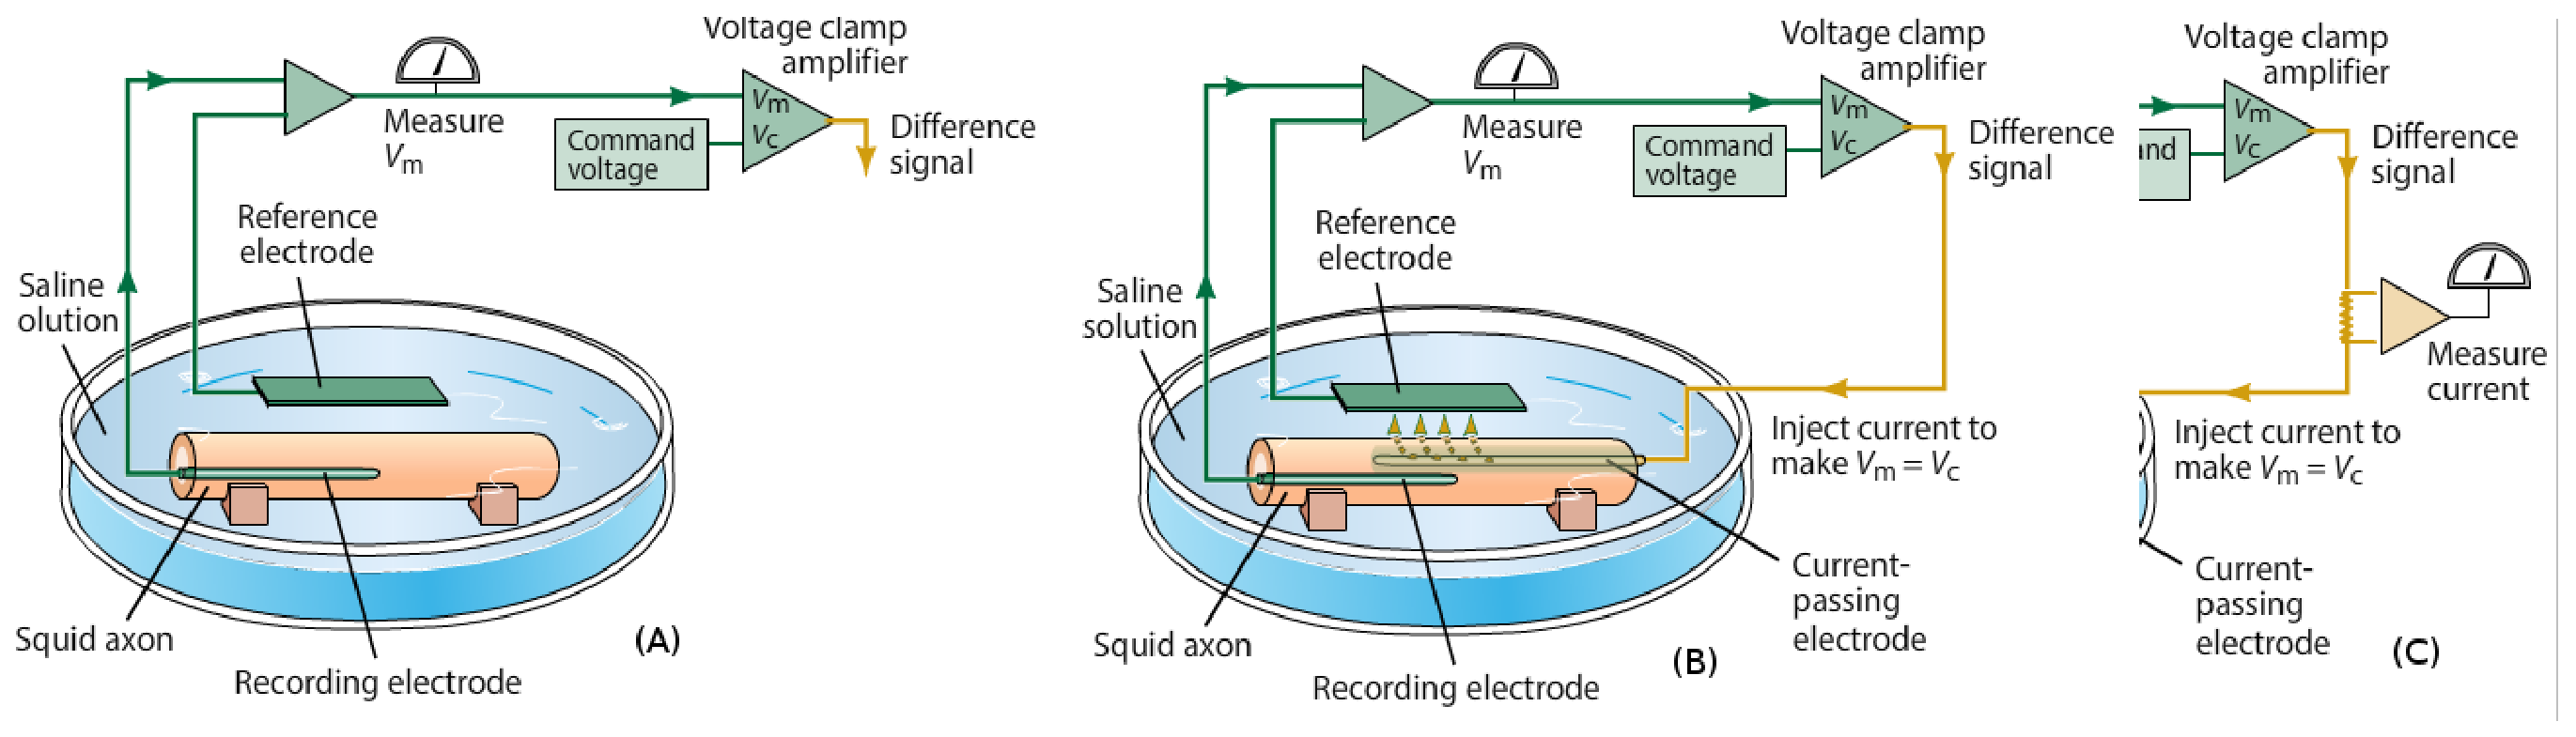
\includegraphics[height=4cm]{./images/voltage-clamp-HH.eps}}
  \caption{Voltage-clamp of squid giant axon: put
  into a dish containing saline solution}\label{fig:voltage-clamp-HH}
\end{figure}

GOAL: Fix $\Vm$ to a given value $V_\step$
\begin{enumerate}

  \item to amplify and measure the transmembrane potential, a negative-feedback
  op-amp is used (Sect.\ref{sec:op-amp_closed-loop_negative-feedback}), i.e. V-
  is connected to the voltage of value $V_\step$ and Vout is connected back to
  the V- (inverting input) via the feedback resistor of resistance Rf (we call
  it {\it voltage divider}): it greatly reduces the gain of the circuit, and
  help keeping Vout recover from change caused by the noise and is
  equal to Vin, which is Vp in Fig.\ref{fig:op-amp-voltage-clamp-circuit}(e).
  The negative feedback is not instantaneous.

  \item an electrode with resistance Re ({\it series resistance}, access
  resistance) is connected one end to the input V+ of the op-amp, and the other
  end injected inside of the cell,
  Fig.\ref{fig:op-amp-voltage-clamp-circuit}(e).

   \item input resistance - Sect.\ref{sec:input-resistance}

\end{enumerate}

\begin{figure}[htb]
  \centerline{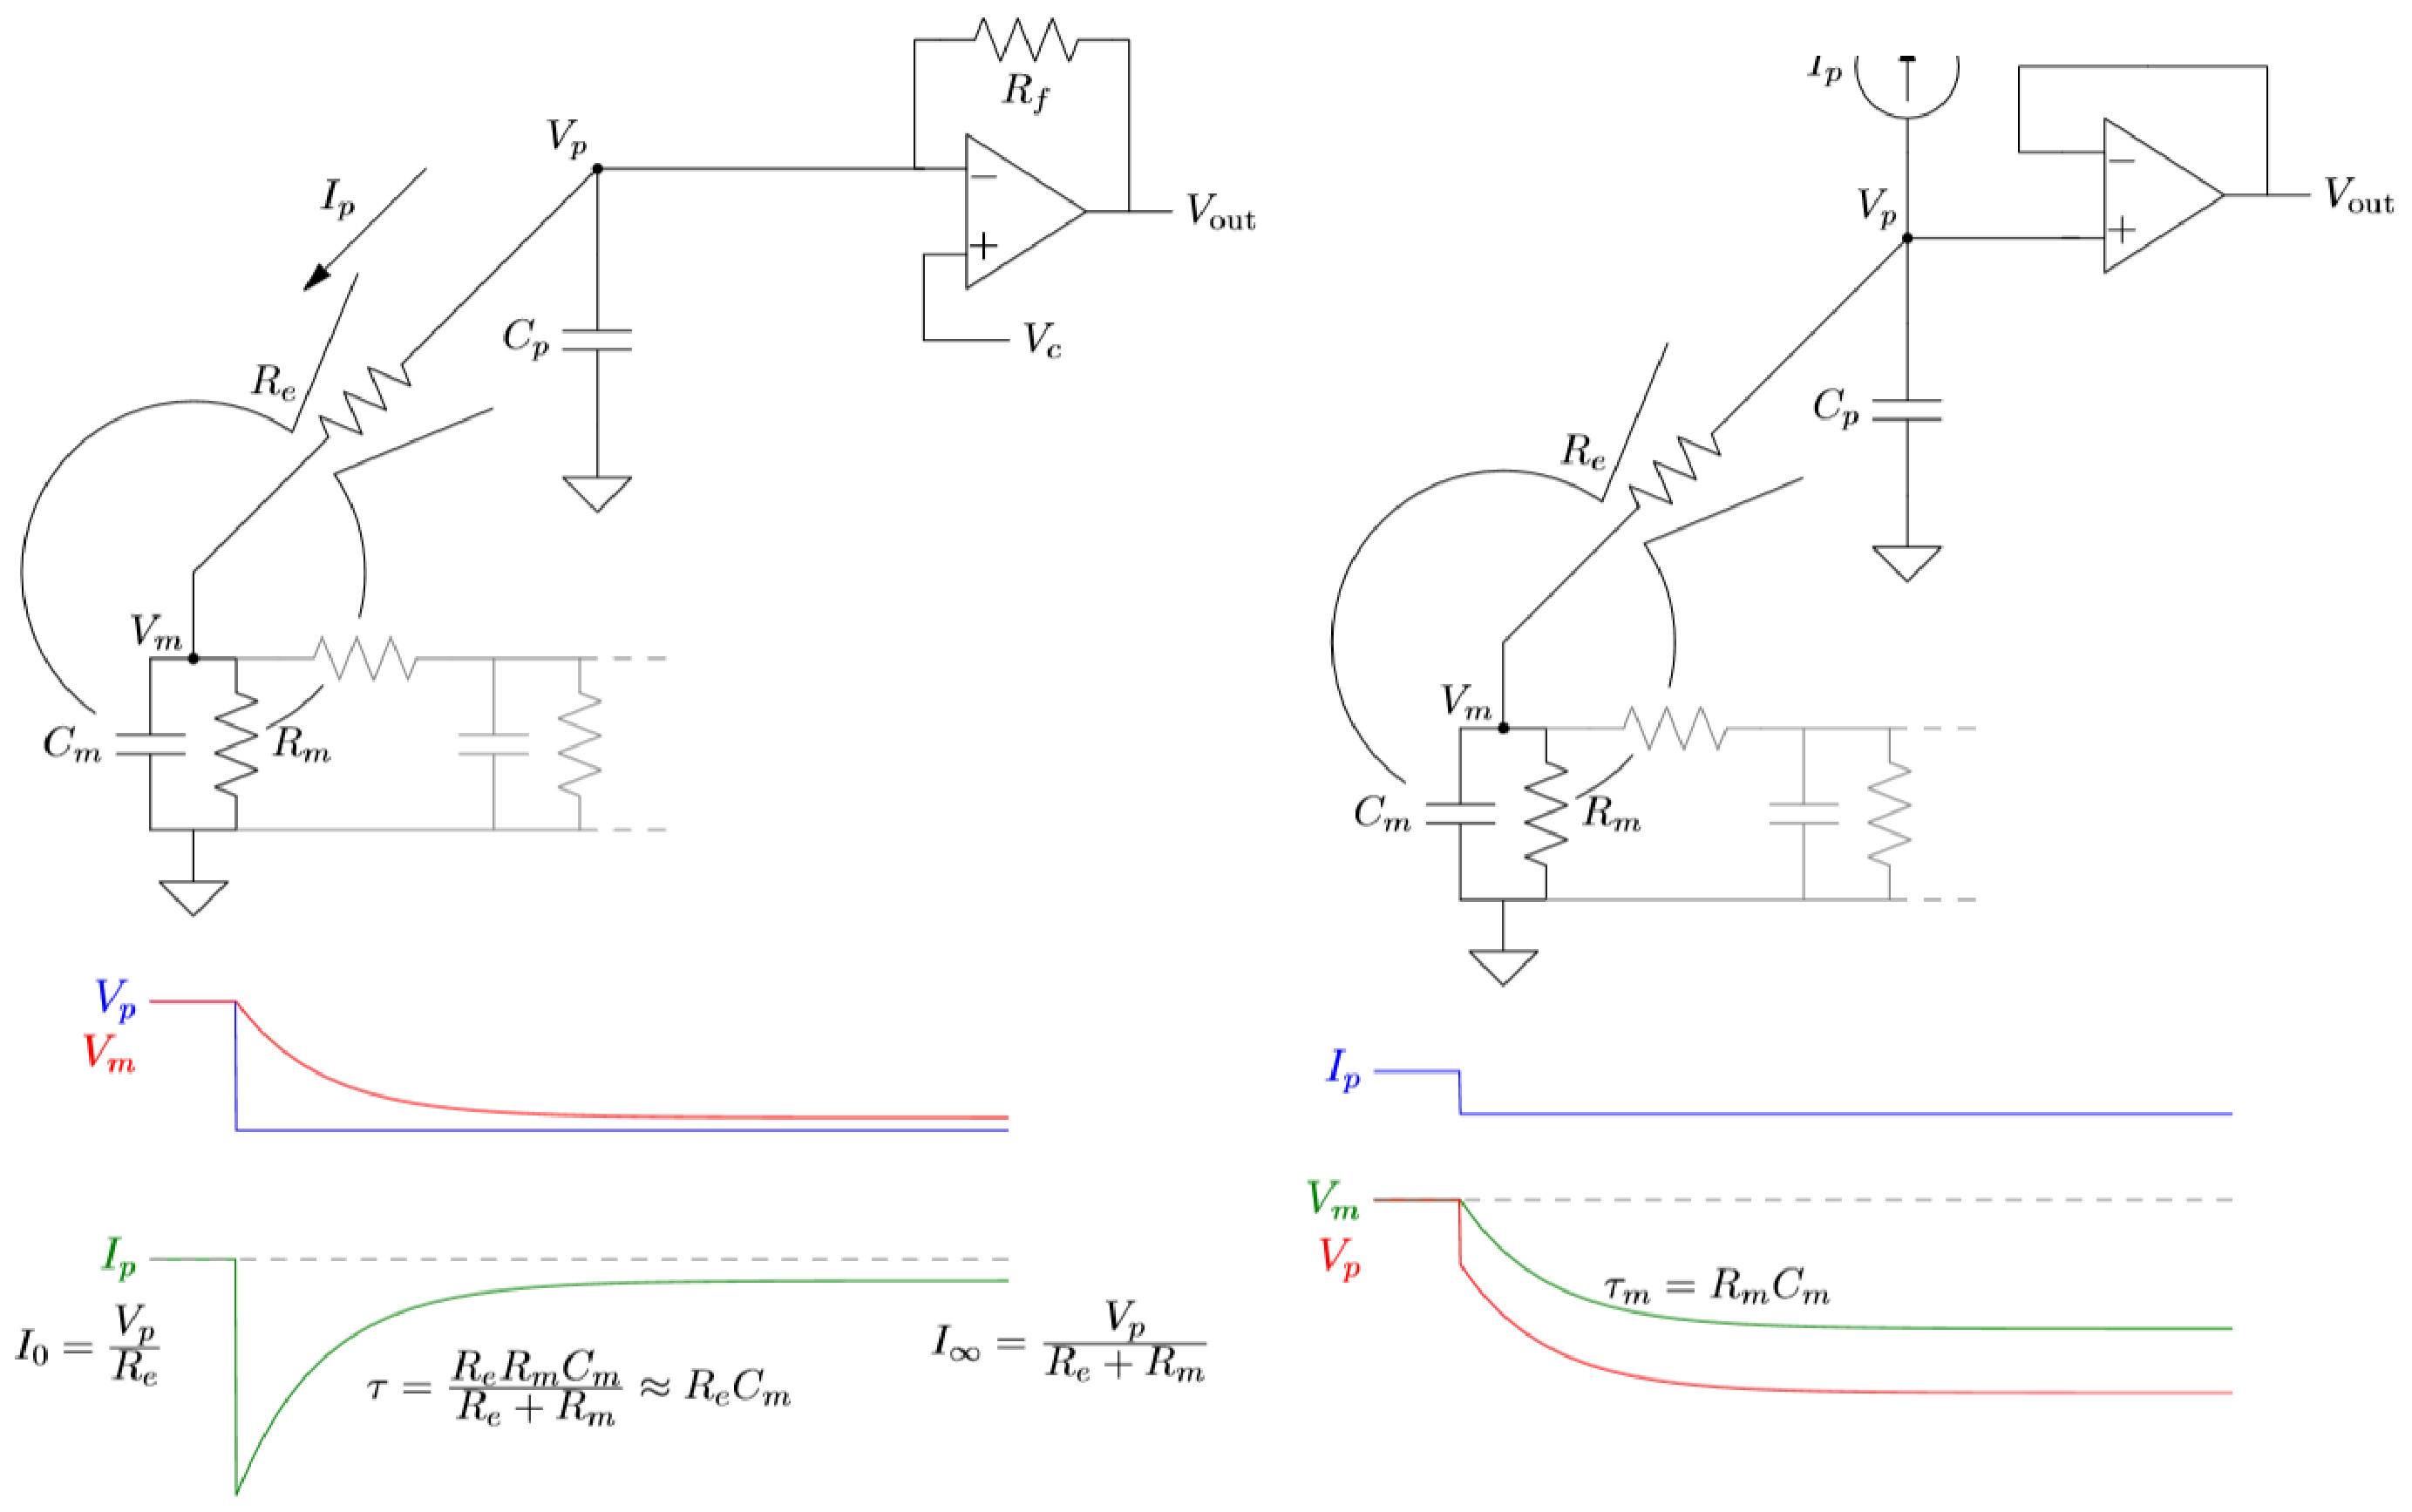
\includegraphics[height=5cm]{./images/op-amp-voltage-clamp-circuit.eps}}
  \caption{(A) voltage clamp; (B) }
  \label{fig:op-amp-voltage-clamp-circuit}
\end{figure}


\begin{enumerate}
  \item first electrode (crossing the membrane):

This internal recording is inserted into the axon (V+), a reference electrode is
put into the bath (V-): the difference signal $\Vm$ is amplified by the op-amp
(Sect.\ref{sec:op-amp}) to be detectable. A second op-amp is used, with $\Vm$ as
V+, and a voltage clamp $V_c$ as V-.

  \item second electrode (cross the membrane): provide injected current
  $I_\inj$,

To ensure $\Vm = V_c$ or keeping $\Vm$ as closed to $V_c$ as possible (i.e.
clamp $\Vm$ with a command-voltage value), the difference signal is used to
generate a current that is injected into the axon,
Fig.\ref{fig:voltage-clamp-HH}(B).

\end{enumerate}

This mored advanced clamp device using two electrodes can avoid electrode
polarization (or current loss due to passing through the electrode),
Fig.\ref{fig:voltage-clamp-HH}, i.e. there is no sag in the outward current.

Hodgkin and Huxley was then able to perform a crucial step of a complete
description of the time- and voltage-dependence of the ionic currents.

\subsection{-- experiment 1: overshoot is a function of sodium current}

By changing external sodium concentration, Hodgkin-Huxley showed that it
affects the height of the action potential overshoot of zero.

\subsection{-- experiment 2}

They used specific blocking agents to dissect out the currents that underline
the action potential, Fig.\ref{fig:HH-experiment-dissect-currents}
\begin{itemize}
  \item Tetrodotoxin (TTX) blocks $\Na$ currents (Sect.\ref{sec:tetrodotoxin})

Since $\Na$ current is an inward current dependent upon extracellular sodium
concentration, this current can be eliminated by removing all external sodium.
This is similar to using TTX, with a major exception - there is an initial
outward surge. EXPLAIN: Even without $[\Na]_o$, there is still $[\Na]_i$, which
can flow outward, down its concentration gradient, through the open $\Na$
channels, Fig.\ref{fig:HH-experiment-dissect-currents}(C).

  \item Tetraethylammonium (TEA) blocks $\K$ currents
  (Sect.\ref{sec:tetraethylammonium})

  \item Chloride conductance was eliminated by replacement of chloride with
  methylsulfonate.
\end{itemize}

\begin{figure}[htb]
  \centerline{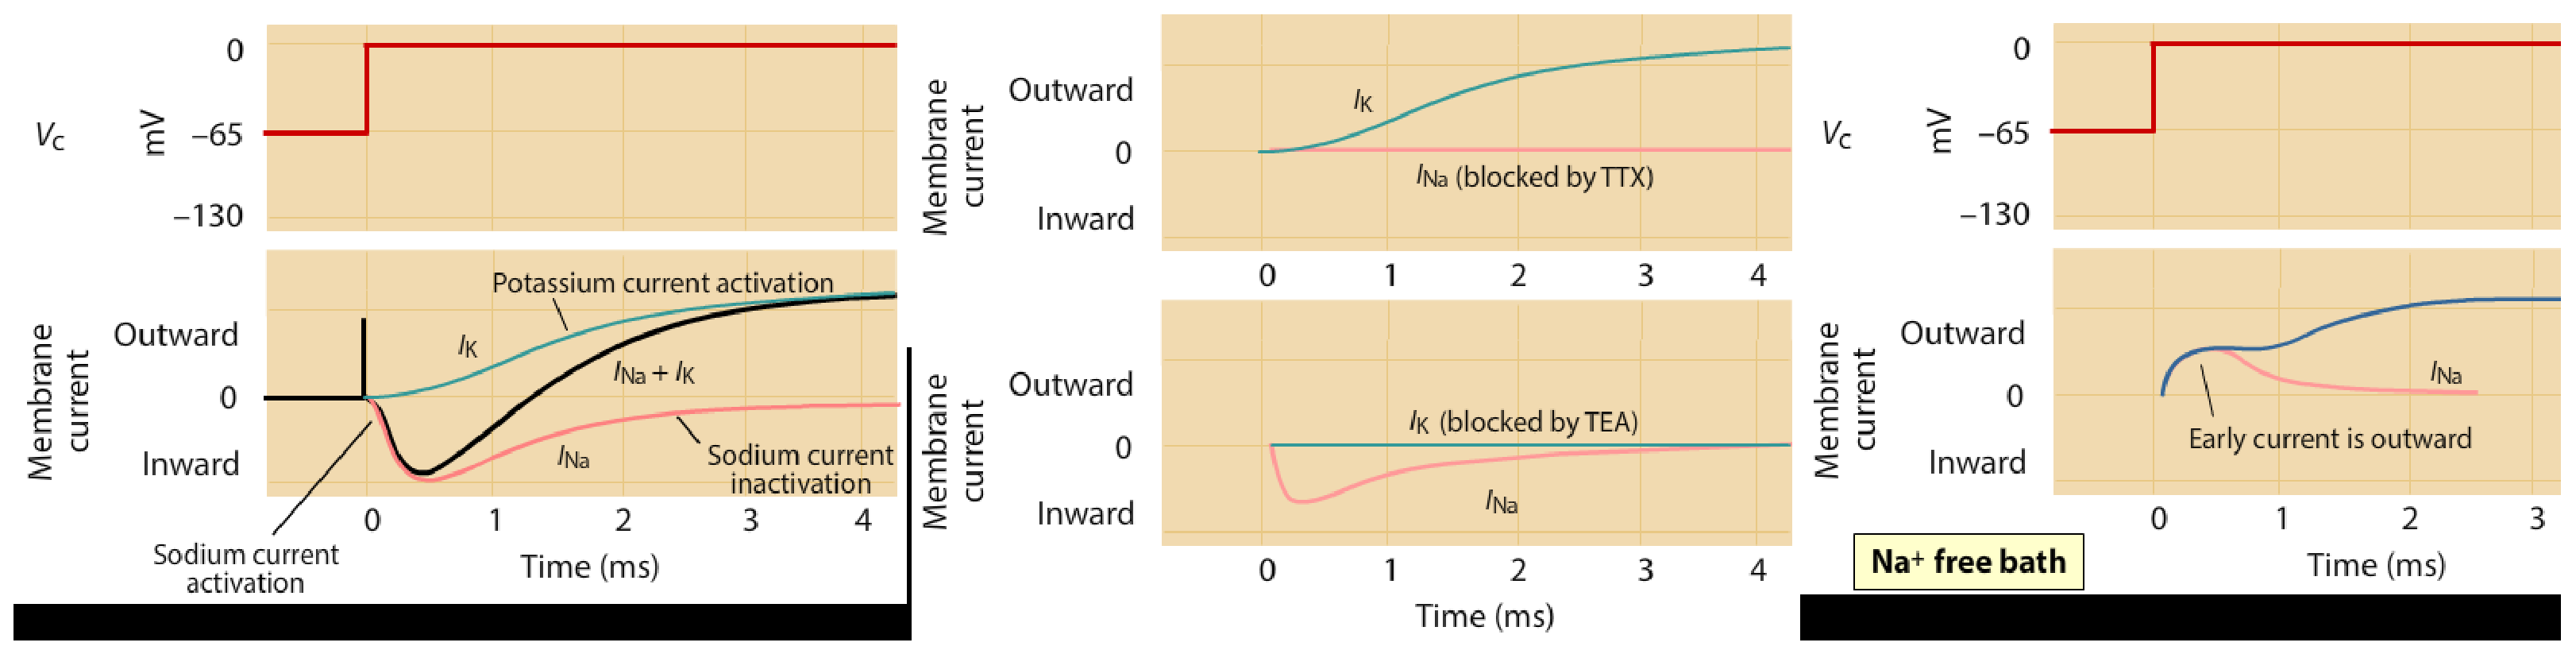
\includegraphics[height=3cm]{./images/HH-experiment-dissect-currents.eps}}
  \caption{Dissecting the two components $\Na$ and $\K$ channels in squid giant
  axon\footnote{\url{http://www.sumanasinc.com/webcontent/animations/content/voltage_clamp.html}}}
  \label{fig:HH-experiment-dissect-currents}
\end{figure}

This  inward current caused by opening of $\Na$ channels is transient, turning
on and then off in spite of the fact that the voltage remains constant.
IMPORTANT: the speed of the onset of the early current, its magnitude, and even
its direction (changing from inward to outward at strong depolarizations) are
voltage-dependent.



% \begin{figure}[hbtp]
%   \centerline{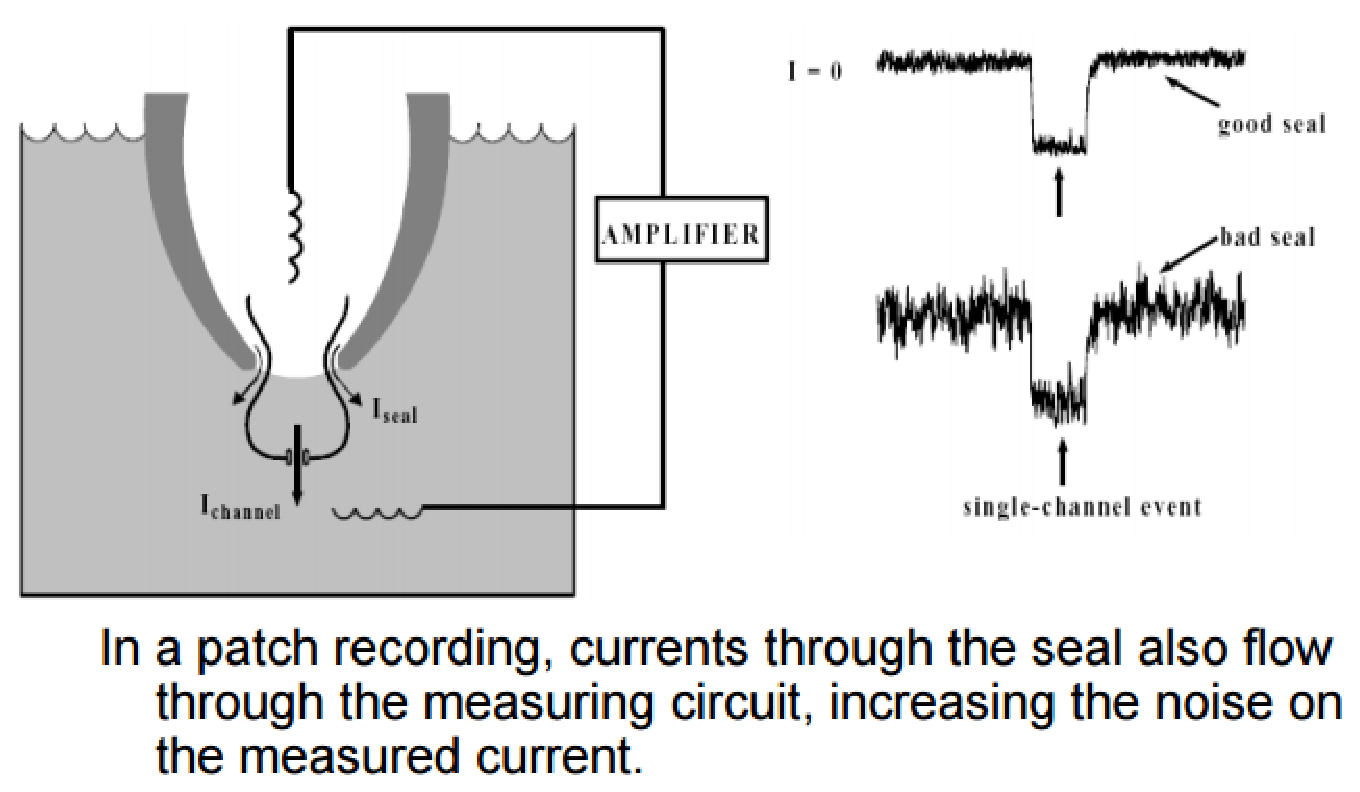
\includegraphics[height=5cm,
%     angle=0]{./images/pipete-seal-leaky.eps}}
% \caption{Good and Bad seal in single channel recordings; in single channel
% recording, the current through the seal $I_\text{seal}$ also recorded as part of
% the $I_\text{channel}$, increasing the noise on the measured current}
% \end{figure}


Based on Ohm's law
\begin{equation}
I = \frac{V_m}{R}
\end{equation}
it's apparent that
\begin{itemize}
  \item  the larger the voltage, the larger the current. However, this
is not always the case for ionic channels, due to both $V_m$-dependent
activation and inactivation.

  \item the larger the resistance, the smaller the current.

\end{itemize}


% In the late 1940s, micro-electrode techniques for the measurement of
% intracellular potentials in single nerve and muscle fibre were made available
% (Sect.\ref{sec:micro-electrodes}).

There are two commonly used voltage-clamp protocols
\begin{itemize}
  \item single-step - Sect.\ref{sec:voltage-clamp-single-pulse}
  \item double-step - Sect.\ref{sec:voltage-clamp-double-pulse}
\end{itemize}
Any change in current over time reflects changes in resistance, i.e., the
opening and closing of ion channel.

\subsection{Sucrose-gap techniques (1954)}
\label{sec:sucr-gap-techn}

The sucrose-gap technique (single gap) was introduced in 1954 by Robert Stampfli
(who worked with Hodgkin and Huxley in 1947-1949).
The sucrose gap technique improves CAP recording by replacing the extracellular
solution between the recording electrodes with a non-conductive sucrose solution
to minimize extracellular shunting.


A chamber holding sucrose solution is applied to the extracellular space,
wrapping around a segment of the nerve fiber is used. As sucrose solution has
the high resistance, a conduction block is created, i.e. forming a gap, and thus
reduces the amount of conducting medium outside of the cell. Thus, making the
recording of currents moving along nerve fibers become more easily. It is useful
in the study of small nerve fibers and electrically connected cells such as
smooth muscle cell.

The nerve fiber is put into a 3 chambers/nodes apparatus, in that the center
node is the sucrose gap. The potential differences is measured between the two
segments separated by the sucrose gap, can be used to infer the axial current.

\begin{enumerate}

  \item {\bf test chamber} (test node): contains physiological solution - mimics
  the ion concentration and osmotic pressure of the cell's natural environment

NOTE: Test drugs can be applied to this chamber. Ag-AgCl or platinum wire
electrode is used to stimulus the cell/nerve fiber in this chamber.

  \item {\bf sucrose chamber} (or gap) - intermediate between the first and
  third chamber: contain an isotonic extracellular sucrose solution of a high
  specific resistance.

This prevent the extracellular current, and thus only intracellular axial
current. This enable proper recording of the potential difference between the
first and third chamber.

  \item {\bf third chamber} (potassium-rich chamber): contains a KCl solution
  that mimics the intracellular solution.

The extracellular sucrose solution has very low conductivity and thus two
flowing streams of sucrose could be used as the "guard" regions in a chamber,
isolating a short, central segment of bare axon. Also, each end of the axon was
bathed in a pool of isotonic KCl solution to eliminate membrane potentials
there.
\end{enumerate}
Basically, the high concentration of sucrose is applied to the extracellular
space, which prevents the correct opening/closing of $\Na$ and $\K$ channels on
the membrane in that region; and increases the resistance between two groups of
cells. This allows all of the current originating on one side of the gap to flow to the
other side only through the interior of the nerve or tissue.

With the sucrose-gap technique the amplitude of the recorded current depends
critically on the ratio of intra- to extracellular longitudinal resistance.


\begin{figure}[hbt]
 \centerline{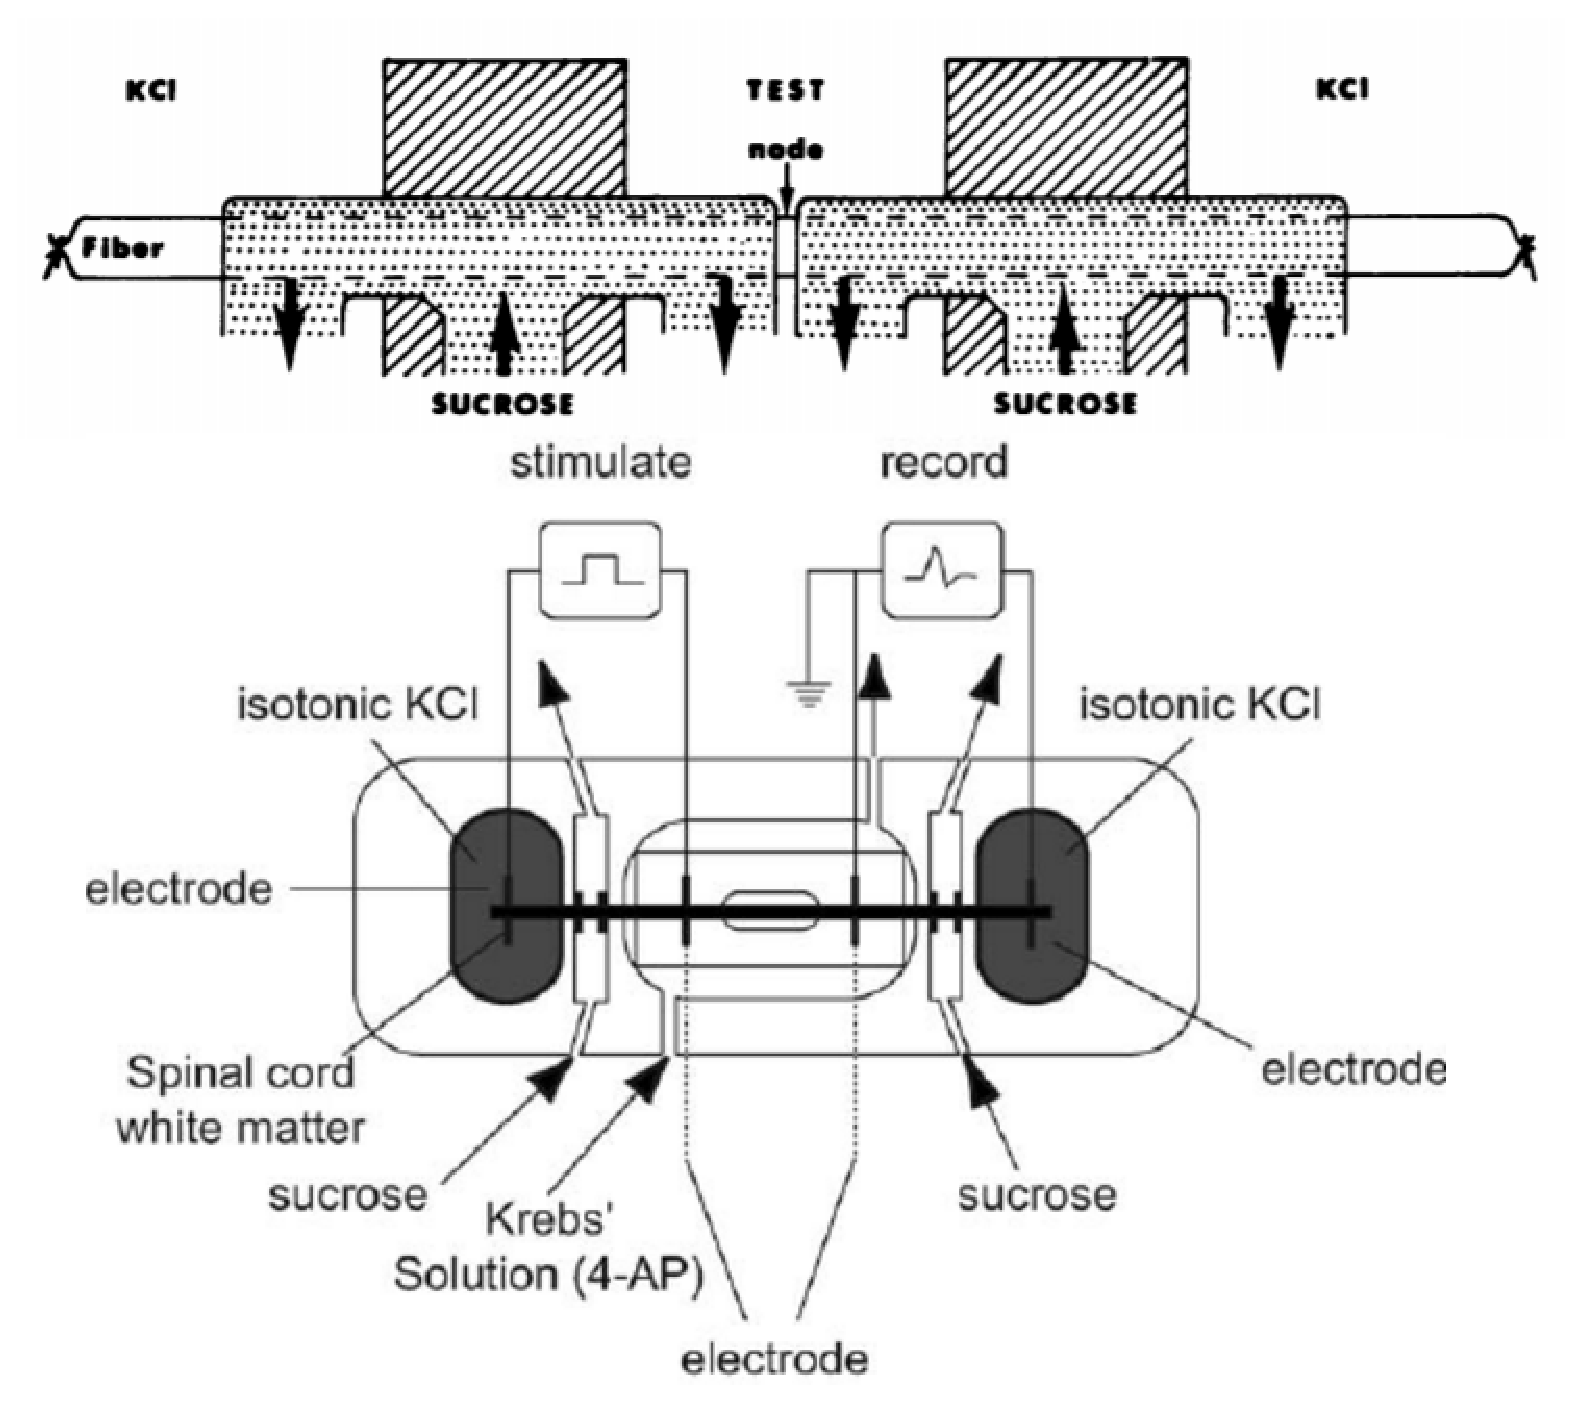
\includegraphics[height=5cm]{./images/double-sucrose-gap.eps}}
 \caption{Double sucrose-gap device}
\label{fig:double-sucrose-gap}
\end{figure}

\subsection{Double sucrose-gap technique}
\label{sec:double-sucrose-gap-technique}

\textcolor{red}{Double sucrose-gap technique:}
chambers containing sucrose solutions are used to isolate a segment of the nerve
or it is used to measure resistance and membrane potential at the same time. Two
tissue, which is immersed in a physiological solution. The two ends of the nerve
or tissue are depolarized by a solution rich in potassium ions.
The double sucrose gap can be used as a voltage clamp as well.


The sucrose-gap technique has been widely used as a convenient tool for
recording of the membrane activities from myelinated or unmyelinated nerves and
muscle preparations (such as smooth and cardiac muscles). The quantitative
measurements of membrane and action potentials in preparations with electrical
coupling between their compartments are made much easier by this technique; the
recorded potentials are rather similar to those recorded with a microelectrode.
%https://www.researchgate.net/publication/247389290_Sucrose-gap_technique_Advantages_and_limitations


A double sucrose-gap is generally advantageous when used to electrically isolate
smaller segments of nerve fibers than would be possible with a single
sucrose-gap. The double sucrose-gap technique is also utilized over the single
sucrose-gap to study cardiac muscle, to provide better clear resolution of early
currents, those occurring within the first 10-100 milliseconds of
depolarization.

Moore, with Fred Julian and David Goldman (1962) adopted sucrose-gap technique
to make voltage clamp. This was first applied to perform voltage-clamp on frog
atrial heart.

[Rouqier O., Vassort G., Stampfli R. (1968) Voltage clamp experiments on frog
atrial heart muscle fibres with the sucrose gap technique. Pflugers Arch Gesamte
Physiol Menschen Tiere. 301(2):91-108]





% \subsection{Double microelectrode techniques}
% \label{sec:double-micr-techn}
% 
% Better than sucrose-gap technique: (1) avoid the problem of shunt
% resistance.

\subsection{Single-electrode (microelectrode) voltage clamp}
\label{sec:voltage-clamp-single-electrode}

The major disadvantage of Hodgkin-Huxley's double-electrode voltage clamp
technique (Sect.\ref{sec:voltage-clamp-hodgkin-huxley}) is its requirement for
double impalement of the cell, i.e. disrupt the cell membrane twice with 2
different electrodes: one to inject charge particles (current pulses) and one to
measure the potential change (inside vs. outside: $\Delta V_m$) -
Sect.\ref{sec:injected-current}. This restricts its application to rather large
cells (>20 $\mum$) and prevents study of cells embedded in tissue.

In an attempt to solve this limitation, single-electrode switching amplifiers
were developed, i.e. one electrode serving double duty as voltage and current
electrode. The electrode switch back and forth between two inputs
\begin{itemize}
  \item  first the amplifier connects its voltage-sensing input
to the electrode, takes a reading, 

  \item and then switch to connecting the current source output to the same
  electrode to deliver current to the cell.
\end{itemize}

{\bf TEMPORAL RESOLUTION}: By switching back and forth between 2 modes, the
technique is limited in its time-resolution, which must be set based on the
cell's RC time constant. 

Cole and Moore (1960) continued to use the axial wire (with the guard ring
technique) to pass current but avoided the complexity of Hodgkin-Huxley's
dual-electrode axial cannula by using the recently developed {\bf
microelectrode} to measure the voltage just inside the membrane.

An electronic switch inside the electrode rapidly switches the wire to the
electrode between a stimulator delivering the current pulses and an amplifier to
measure the change in potential. For short periods of time, the amplifier
connects its voltage-sensing input to the electrode, takes a reading, and
subsequently connects the current source output to the same electrode to deliver
current to the cell

The high frequency of switching requires a low capacitance electrode, as the
time at one mode needs to be longer than the time capacitive current is removed.
This approach, however, is limited in its time-resolution by the switching
frequency between the two modes, which must be set based on the cell's RC time
constant (the product of cell's input resistance and capacitance).


\subsection{* Whole-cell patch clamp: whole-cell ruptured patch-clamp,
whole-cell perforated patch-clamp, whole-cell loose patch-clamp}
\label{sec:patch-clamp-whole-cell}



\subsection{-- whole-cell ruptured patch-clamp}
\label{sec:whole-cell-patch-clamp-Giga-Ohm}

Whole-cell {\bf ruptured patch-clamp}: The pipette is left in place on
the cell to form the GigaOhm seal but more suction is applied to rupture the membrane
patch.

\subsection{-- whole-cell outside-out patch-clamp}

Whole-cell outside-out patch-clamp (see in patch outside-out
patch-clamp)

The latter approach has an advantage of reusable the patch with different
solutions since the binding sites of the ligand-gated channels are mainly
located on the extracellular side of the membranes.
Also, as the composition of the intracellular is lost with the outside-out
configuration, the 'not physiological conditions' of this approach may not give
accurate records of {\it in vivo} ion channels behavior.
However, there are situations that we need to use outside-out configuration,
e.g. concentration jump or voltage jump experiments to recorded data (see
Sect.\ref{sec:GlyR_example})

Most whole-cell voltage-clamp measurements are made with a patch-clamp headstage
amplifier configured with a 500 M$\Omega$ feedback resistor allowing to measure
currents of up to 20 nA, Fig.\ref{fig:patch-clamp}.
\begin{itemize}
  \item In 5 kHz bandwidth, the resistor alone produces about 400 fA rms noise
\end{itemize}
NOTE: A low gain 50 M$\Omega$ headstage can pass currents of up to 200 nA.

Other offshoots of the patch pipet technique are the loose patch, the perforated
patch, as well as the recording from macropatches and the patch-cram detection
technique. Perhaps the recent developments in the patch-clamp field with the
biggest impact are the combination of two of the most powerful life science
technologies: molecular biology and imaging. This led to the intertwining of the
patch pipet with RT-PCR (Sect.\ref{sec:RT-PCR}) and fluorometric techniques.

It records the currents through multiple channels at once, over the membrane of
the entire cell, Fig.\ref{fig:whole-cell-patch-clamp}. At whole-cell recording,
there are two patch-clamp approaches:
\begin{enumerate}
  \item ruptured patch-clamp
  \item outside-out patch-clamp
  \item inside-out patch-clamp
  \item loose patch-clamp
\end{enumerate}

\begin{figure}[hbtp]
  \centerline{\includegraphics[height=5cm,
  angle=0]{./images/whole-cell-patch-clamp.eps}} \caption{Whole-cell patch clamp
  for cardiac myocytes. The interior of the pipette is filled with either high
  Sodium chloride or potassium chloride solution. An electrode (chloried silver
  wire) connects the pipette solution to the head stage of an electronical
  amplifier. The amplifier is connected in the circuit so that the current
  flowing through the ion channel is measured as a voltage drop. A second
  choride silver wire is inserted into the bath around the cell and serves as a
  ground electrode.}
  \label{fig:whole-cell-patch-clamp}
%\url{https://www.haikudeck.com/the-patch-clamp-method-education-presentation-FnnhmtwzqX#slide-7}
\end{figure}


\subsection{-- whole-cell inside-out patch-clamp}

Whole-cell {\bf perforated patch-clamp}: The pipette is left in place on the
cell to form the GigaOhm seal; yet suction is not used to rupture the membrane.
Instead, the electrode solution contains small amounts of an antifungal or
antibiotic agent, such as amphothericin-B, nystatin, or gramicidin, which
diffuses into the membrane patch and forms small pores in the membrane,
providing electrical access to the cell interior.

Perforated patch-clamp allows recording a more stable AP by minimizing
intracellular dialysis and ionic current rundown \citep{ishibashi2012}.

\subsection{-- whole-cell loose patch-clamp}

Whole-cell {\bf loose patch-clamp}: Instead
of forming a tight G$\Ohm$ seal, loose patch forms a loose seal (low electrical
resistane). The lack of a tight seal creates a small gap through which ions can
pass outside the cell without entering the pipette.
It also allows (1) the micro-pipette to be removed from the cell after
recording, without breaking the membrane (repeated measurements in a variety of
locations on the same cell without destroying the integrity of the membrane),
(2) studying muscle cells as they contract under real physiological conditions,
(3) obtaining recordings quickly.

To form a loose seal, the pipette is moved slowly towards the cell, until the
electrical resistance of the contact between the cell and the pipette increases
to a few times greater resistance than that of the electrode alone.

Loose patch-clamp nowadays can resolve currents smaller than 1 mA/cm$^2$.

\subsection{Dynamic clamp}
\label{sec:dynamic-clamp}

Consider the current clamp (Sect.\ref{sec:current-clamp-protocol})
\begin{equation}
\Csc \frac{dV_m}{dt} = -\sum I_\text{ion} + I_\inj
\end{equation}
in that the injected current can be completely independent from the
transmembrane potential $\Vm$.

In {\bf dynamic clamp} protocol, we impose a loop in that $I_\inj(\Vm)$.
The above equation is strictly equivalent to the 'additional' current of
conductance $-g_\text{add}$ with reversal potential $E_\text{add}$
\begin{equation}
\Csc \frac{dV_m}{dt} = -\sum I_\text{ion} - g_\text{add}(V_m - E_\text{add})
\end{equation}

This is exactly what happens in a dynamic clamp protocol, i.e. a loop between
injected current as a function of the current transmembrane potential.

The dynamic clamp is a novel method that uses computer simulation to introduce
artificial conductances into cells to simulate electrical coupling,
votage-dependent, leak, and synaptic conductances.  This approach makes computer
simulation an interactive experimental tool.

Since $g_\text{add}$ is time-dependent, it can be negative; and we can model any
waveform of $g_\text{add}$. This provides a way to cancel out the effect of a
given ion channel types. $g_\text{add}$	 has to be calculated in real time, e.g.
assuming the NaT channel follow the Hodgkin-Huxley formula 
(Sect.\ref{sec:NaT-current})

% TODO: update this section dynamic clamp

\section{Information}
\subsection{Why?}
\label{sec:why}

As most ion channels on the membrane are voltage-gate channels, it is the
voltage that determines the membrane permeability, not the trans-membrane
currents. In nerve cells, the action potential (AP) is determined mainly by the
two types of ion channels, sodium and potassium. The sodium conductance
activates rapidly and drives the rising phase of the AP while the potassium
conductance activate slowly and contribute to the falling phase of the AP, as
shown in
Fig.~\ref{fig:AP_diagram}\footnote{\url{http://www.sumanasinc.com/webcontent/animations/content/voltage_clamp.html}}.

\begin{figure}[htb]
  \centerline{\includegraphics[height=6cm]{./images/AP_diagram.eps}}
  \caption{Voltage clamp for squid axon}\label{fig:AP_diagram}
\end{figure}

One difficulty when studying the ionic permeability (the conductances)
is that they're changing over time and with voltage. The idea is that
it would be easier if we can control (or clamp) one free parameter,
e.g. the voltage and see how the conductances change over time
only. This is the core idea of a technique called {\it voltage clamp}.

By fixing the voltage across the membrane, one can analyse the change
in conductance (or electric current) through each type of channel
easily. The voltage clamp was invented by Kenneth Cole (1940s) and
applied by Hodgkin et al. (1952) to measure squid giant axons'
electrical
current\footnote{\url{http://www.scholarpedia.org/article/Voltage_clamp}}.
This is a negative electronic feedback device that adjusts the applied
current $I_{app}$ to match and counter the membrane currents such that
the membrane voltage is held constant (clamped) at any desired level
\footnote{\url{http://www.ncbi.nlm.nih.gov/books/bv.fcgi?rid=neurosci.box.174}}.

{\bf Why holding the voltage constant for a certain period of time is
important?} In a biological system, the transporation of ions across the
biological membrane occurs throught the channels pore of certain types of ion
channels whose gating (opening or closed) is governed by the change in voltage.
So, the best way to characterize this voltage-dependency
is to use voltage-clamp protocols.

\subsection{Theory}
\label{sec:theory}

The membrane is assumed to function as a capacitor and the current
through the membrane is composed of the ionic current and the
capacitive current
\begin{equation}
  \label{eq:158}
  I_m = I_{ion} + C\frac{dV}{dt}
\end{equation}
The voltage is usually forced to change in a squared stepwise fashion,
i.e. being change as rapidly as possible from one steady level to
another.

\subsection{Experiment}
\label{sec:experiment}


\begin{figure}[htb]
  \centerline{\includegraphics[height=4cm]{./images/voltage_clamp.eps}}
  \caption{Voltage clamp for squid axon}\label{fig:voltage_clamp}
\end{figure}

A neuron to be examined is placed in a dish of saline solution, as
shown in Fig. \ref{fig:voltage_clamp}. One electrode is inserted
inside the axon, one is put in the solution as an external reference
(bath) electrode. Then, the voltage difference $V_m$ across the
membrane is measured.

$V_m$ is then being used to compare with the voltage to be controlled
(called {\it command voltage}) $V_c=E$. If the two voltages are
different, the comparator fire a difference signal.
The voltage clamp
amplifier will magnify to a scale factor $A$ and generate a current
that is injected into the axon by a third electrode (called
{\it current-passing electrode}).

\begin{equation}
  \label{eq:159}
  V_0 = A(V_m-V_c)
\end{equation}
This potential difference pass currents through an access resistance
$R_a$ and pass through the membrane and adjust the membrane potential
\begin{equation}
  \label{eq:160}
  V_m = V_0 + R_aI_{app}
\end{equation}

This current $I_{app}$ aims to adjust $V_m$ so that its feedback keep
$V_m$ as closed to $V_c$ as possible.  The amount of applied current
$I_{app}$ can be recorded and analyzed.

Substituting for $V_0$, we have the controlled expression for $V_m$
\begin{equation}
  \label{eq:161}
  V_m = V_c\frac{A}{1+A} -\frac{R_aI_{app}}{I+A}
\end{equation}
Clearly, as the gain $A$ increases, the membrane potential approaches
the command potential, and the effect of the access resistance is reduced.



\begin{figure}[htb]
  \centerline{\includegraphics[height=6cm]{./images/voltage_clamp_schematic.eps}}
  \caption{Simplified schematic of voltage
    clamp}\label{fig:voltage_clamp_schematic}
\end{figure}

\subsection{Examples}
\label{sec:examples}

Suppose $V_c$ and $V_m$ are identical and equal to -65mV. Then there
is no injecting current into the axon. As a result, there is no change
in the membrane potential.

What if we impose a new voltage to the control $V_c = 0$mV? The
comparator then fire an electrical current
\begin{equation}
  \label{eq:162}
  I_{app} = \frac{V_m-V_0}{R_a}
\end{equation}


{\bf REMARK}:

\begin{itemize}
\item
In this method, the channel behavior is obtained using
current measured from an area of membrane with a uniform, controlled
voltage than when the voltage is changing freely with time and between
different regions of the cells.

\item
This method is applied to measure whole cell or large area of membrane
containing hundreds of ion channels. Such current is called
{\it macroscopic currents}. In order to study a single channel, we use
a newer technique, {\it patch-clamp}.
\end{itemize}

\subsection{Currents in a voltage clamp}
\label{sec:voltage-clamp-current-components}

A typical record resulting from the application of a step change in membrane
potential is shown in Fig.\ref{fig:voltage_clamp_ex} with upto 4 components.

\begin{itemize}
  \item the current trace being used for fitting is the average of a number of
  traces

Example: each current trace was an average of three consecutive
records elicited at 0.3 Hz
  
  \item the unexpected components (capacitive current and leak current) are then
  subtracted from the trace recorded using a hyperpolarizing current (which is
  expected to show the change of current via these two components)

\begin{enumerate}
  \item the transient component ({\bf capacitive current}): This initial
  capacitive surge is completed in about 20$\mu$sec, corresponding to the
  presence of a capacitor - Sect.\ref{sec:capacitive-current}.

At the transient change in control voltage, there is a transient
change in capacitive current followed by a characteristic pattern of
inward and outward current, as shown in Fig.~\ref{fig:voltage_clamp_ex}.
This capacitive current needs to be subtracted from the recorded trace if
present - Sect.\ref{sec:capacitive-current-subtraction}.

This current drops to zero before the ionic current becomes significant.

  \item an early inward current:
  this is the  result of experimental error (insufficient clamp, clamp ringing,
  capacitive surge, etc.).


An example of error is:  this initial flow of ionic current arising from a
trans-threshold voltage step is due to $\Na$ influx.

The net driving force of this $\Na$ influx is the difference between the step
potential and the sodium Nernst potential (Sect.\ref{sec:nernst-equation}) of
about +57 mV. Example: $V_s = +20$ mV, then $(V_s - E_\rev) = -37$ mV. Since
this is negative, it is inward, i.e a result inward (sodium) current is
expected. The elevated sodium permeability is transitory, i.e. quickly decay.
As the $\Na$ permeability falls, the $\K$ permeability rises and remain
elevated.

REMEMBER: This can be the small amout of $\na$ ion influx via
$\K$ channels.

  \item an (rise to asymptotic) outward current: this can be outward of $\K$
  current

The driving force is $(V_s - E_\rev(\K))$. If $V_s = +20$mV and
$E_\rev(\K)=-70$mV, then the driving force is $(20 - (-70))=+90$mV, i.e. the
strong outward current.

\end{enumerate}
\url{http://www4.ncsu.edu/~msolufse/Currents.pdf}
  

  
  \item the resulting membrane current trace were then filtered using an
  eight-pole Bessel lowpass filter (4 kHz, 3 dB, VBF8, Kemo Ltd, Beckenham, UK) 
\end{itemize}



\begin{figure}[htb]
  \centerline{\includegraphics[height=6cm]{./images/voltage_clamp_ex1.eps}}
  \caption{Voltage clamp}\label{fig:voltage_clamp_ex}
\end{figure}



\subsection{Separate currents in a voltage clamp}
\label{sec:voltage-clamp-separate-current-components}

A problem given in Sect.\ref{sec:voltage-clamp-current-components} makes it hard
to extract the current from a specific ion channel. In many cases, ionic
substitution can be used.

However, ionic substitution alone cannot be used to separate currents through
different channels that permeate the same ions, e.g. different types of $\K$
channels. To study individual type of ion channel, we can use specific agents to
block the corresponding type of ion channels. E.g. Tetrodotoxin (TTX) specify
blocks sodium channels. Tetrathylammonium (TEA) specify blocks potassium channels.

$\Ca$ ion also poses different problems as $\Ca$ entry may activate other ion
channels (e.g. $\Ca$-dependent $\K$ channels and $\Cl$ channels); and because
replacement of $\Ca$ with other ions, e.g. with $\Ba$, can shift
voltage-dependence of gating many ion channels.

Another way to get rid of unexpected ion channels, is using a dynamic clamp
(Sect.\ref{sec:dynamic-clamp}) which inject a current, that is expected
to be of the same magnitude but of different direction of the current
that we want to get rid of.





\subsection{-- Series resistance (Rs) = electrode resistance (Re) = access
resistance: 10-500 MegaOhms (older) to 10 GigaOhms (newer)}
\label{sec:series-resistance}
\label{sec:electrode-resistance}
\label{sec:access-resistance}
\label{sec:microelectrode-filling-solution}
% \subsection{-- series resistance (Rs)}
% \label{sec:series-resistance}
%
%\subsection{electrode resistance (10-500 MegaOhms)}
%\label{sec:electrode-resistance}

A resistance defines how hard/easy the current can pass through.

The resistance $R_e$ of the (tip of an) electrode depends not only on the length
of the electrode shank (e.g. 15mm) and the size of the tip (e.g. outer diameter
of 70nm), but also on the nature of the conductive electrolyte inside the tip
(eg. 3M KCl filling). 

When using in a current clamp (Sect.\ref{sec:current-clamp-protocol}), this
resistance is in series to the RC circuit of the membrane, and is thus also
known as series resistance $R_s$.

Typical resistances of intracellular electrodes to DC-current are 10-500
Megaohms.

{\bf Example}: An electrode with a shank of about 15 mm and with a tip outer
diameter of about 70 nm.
\begin{itemize}
  \item  filled with 3 M KCl filling (typicall): has resistance $R_e$ of 100
  Megaohm 
  
  \item with the neuron-marking solution Lucifer Yellow (5 \% LY with 0.1 \%
LiCl), which has much lower mobility than potassium or chloride ions: has
resistance $R_e$ of 600 MegaOhm or more.
\end{itemize}


\url{https://www.researchgate.net/post/Can_someone_advise_on_series_resistance_in_current_clamp}

\url{http://neurobio.drexelmed.edu/GaoWeb/Resources/Series Resistance Compensation.pdf}

\url{http://www.biologie.ens.fr/~barbour/electronics_for_electrophysiologists.pdf}



\subsection{electrolyte}


The pipette of the electrode is a conductive medium (the electrolyte
filling the pipette, e.g. 1-3 M KCl).  The electrolyte helps to create a
distributed resistor.


\subsection{electrode capacitance (pF) and resistance}
\label{sec:electrode-capacitance}

The glass electrode has also a (distributed) capacitance, which is high enough
(in the range of picoFarads) to define, with the electrode resistance
(Sect.\ref{sec:electrode-resistance}), a large time constant for the electrode
(the time constant $\tau$ = RC).

How fast signals can be recorded (how reliable is the high frequency end of the
spectrum) is determined by how well the electrode capacitance can be
compensated. It is possible to decrease the electrode time constant from the
range of tens of milliseconds to some microseconds.



\subsection{RC of electrolyte-electrode}

Because the resistance (Sect.\ref{sec:electrode-resistance}) and the capacitance
(Sect.\ref{sec:electrode-capacitance}) form together a low-pass filter, the
electrode is inherently very slow, if nothing is done about the problem.


\subsection{tip potential}
\label{sec:tip-potential}

The tip potential is difficult to measure, but this is possible to estimate with
a measurement of the recording electrode against a similar but broken-tipped
specimen.

A glass microelectrode will generate a voltage called a tip potential, when in
contact with any solution, be it intra- or extracellular, artificial or in
tissue. The tip potential may be up to nearly -100 mV.

If the tip potential is the larger, the sharper is the electrode.
The tip potential is formed by two components, the liquid junction potential and
the tip potential proper.
\begin{itemize}
  \item  The tip potential proper is a more mysterious part of the phenomenon.
  It depends on the tip size and shape, but is abolished in symmetrical
  solutions (i.e. when the filling solution and the outside liquid have the same
  components)

  \item
\end{itemize}


 The electrolyte in the pipette, when touching another electrolyte, will form a
Nernst potential-like voltage that is defined by the composition of the
solutions in question.






\subsection{recorded potential}

In routine use the experimenter would use the amplifier's off-set
control to remove the tip potentials, as well as to get rid of other similar
voltages (like the voltage created by the dis-similarity between the recording
and the indifferent electrode).

Exact recording of DC-voltage levels, most notably the cell resting potentials,
may be biased by the tip potentials (Sect.\ref{sec:tip-potential}), although
they have been partially offset from the recordings by electronics.

The recorded voltage contains noise both from the cell membrane and from the
electrode. This is because during recording a small (bias) current flows through
the electrode tip. In addition to this, the glass electrode is especially prone
to pick up 50 Hz (or 60 Hz) hum. This requires some elaborate planning
concerning the grounding of the recording set-up. All that can be done to reduce
electrode capacitance is useful as well, although some theoretically-attractive
techniques, like so-called driven shield (driving the recorded signal to the
immediately surrounding grounded surface in order to eliminate the capacitance),
do not help very much in practice.

\subsection{Whole-cell recording}

Ion channels catalyze the diffusion of ions across membranes with
electrical currents in the order of pico Amperes ($10^{-12}A$). The
recording of single channel currents shows
{\it two current levels corresponding to the closed and open state
  respectively}.
Transitions between these two states are very fast and in the order of
fractions of a millisecond ($10^{-3}s$), and appear in the recordings
as rectangular jumps from one level to the other. The amplitude of the
jump corresponds to the current magnitude. The current can be
normalized and expressed as resistance $R$ (or its inverse, the
conductance $g$) because it is proportional to the membrane potential as
defined by Ohm's law (V = R*I).

% To measure the current level, a common experimental technique is {\bf
%   Voltage clamp}
% Nowadays, there are two major ways to record the kinetics of ion channels:
% (1) whole-cell recording, (2) single-channel.

\begin{itemize}
\item Whole-cell recordings give much more accurate information near
  $E_{rev}$ (Sect.\ref{sec:reversal-potential}), where net current is small; they
  also allow manipulation of ion concentrations on both sides of the membrane with relatively
  little rundown.

\item Single-channel measurements eliminate the uncertainty associated
  with variations in channel gating, a particularly serious problem at negative
  potentials where channel deactivation is rapid.  However, the current and
  dwell-time for a single channel at the negative potential is relatively small.

  This drawback has been resolved with the use of Bay K 8644 and some other
  agonists to increase the proportion of long, well-resolved
  openings~\citep{hess1986ccs} (Sect.\ref{sec:LCC_Hess1984}).
\end{itemize}

% To model correctly the gating of ion channels, there are different methods.
% We'll cover how data are collected, and how to interpreted the data, from that
% a proper kinetics model of ion channel gating can be developed.

\subsection{Macroscopic currents}

In 1982, the first subunit of the nicotinic receptor was cloned
\citep{noda1982}. Also, expression of the receptor in oocytes or cell lines can
be made alllowed the effect of mutations to be tested easily. The widely studied
channels are nicotinic receptor, and glycine receptors. The results from other
channels are still not clearly understood, e.g. glutamate receptors (NMDA)
\citep{colquhoun2002}.

\subsection{Maximum conductance}
\label{sec:maximal-conductance}

An important use of the I-V curve (Sect.\ref{sec:I-V-curve}) is to calculate the
maximum conductance of the whole-cell level by estimating the slope between the
peak-current and the voltage, while fixing the reversal potential as origin,
Fig.\ref{fig:IVcurve_conductance}.

\textcolor{red}{IMPORTANT:} The conductance recorded at $I_{\text{peak}}$ is not
the maximal conductance (as described in
Sect.\ref{sec:peak-conductance-vs-maximal-conductance}). So, to help finding the
maximal conductance at peak current, we find the slope conductance of the peak
current I-V curve in the range
\begin{itemize}
  \item 0 to +40 mV for $\Na$ current (Huguenard, Hamill, Prince (1988))

  \item
\end{itemize}

Example: \citep{lee1999}: From the holding potential -80mV, the different test
pulse of 20ms as applied from -80mV to +35mV in 5mV increment. The next test
pulse is repeated in 5sec interval.  The peak
$I_\na$ at different conditioning pulse voltage are recorded vs. $V_m$
(Sect.\ref{sec:Ina_Lee1999}).

As the extreme point of the I-V curve is near the $V_m = 0$ (mV), the maximum
conductance is $g_\max = \frac{E_\rev}{I} = tan(\alpha) = -1.5 nA / (+60) mV$.
\url{http://amrita.vlab.co.in/?sub=3&brch=212&sim=1309&cnt=1}

\begin{figure}[hbt]
 \centerline{\includegraphics[height=4cm,
 angle=0]{./images/IVcurve_conductance.eps}}
 \caption{The whole-cell conductance is estimated}
\label{fig:IVcurve_conductance}
\end{figure}

\section{Standard voltage-clamp protocol}
\label{sec:voltage-clamp-protocol}

Voltage-clamp techniques enable holding the membrane potential at a command
value. The transmembrane potential is held using a proper
voltage-clamp technique (Sect.\ref{sec:voltage-clamp-techniques}).
The question is how we utilize this technique in understanding gating of
voltage-gated ion channels. Example:
\begin{enumerate}

  \item in excitable cells: voltage-(and/or-ligand) activated conductances

  \item  in neurons: estimate  postsynaptic current (PSC -
  Sect.\ref{sec:postsynaptic-current}).

  By holding the somatic postsynaptic-potential (PSP), we measure transmembrane
  current (Sect.\ref{sec:transmembrane-current}) required to maintain that
  voltage.  Despite the fact that the voltage-clamp does not mimic a process
  found in nature, it is useful
  \begin{enumerate}
    \item eliminate the capacitive current, except for a the current in a brief
    time following a step to a new voltage (Sect.\ref{sec:capacitive-current})

    \item the current that flows (during that brief charging time) are
    proportional to the membrane conductance, i.e. to the number of open channels

    \item it offers the control over the key variable (i.e. the $V_m$) that
    determines the opening and closing of ion channels
  \end{enumerate}

\end{enumerate}

The purpose of a voltage-clamp protocol is to help estimating the kinetics of
activations and inactivation characteristics of voltage-gated ion channels, by
holding the transmembrane potential at different values and switch from one
value to another.

\begin{mdframed}

\textcolor{red}{Usually, the investigator has no inherent interest in the
membrane current, but is interested in the membrane conductance, since
conductance is directly proportional to the ion-channel activity}. 

Current is measured because the investigator has no direct way of measuring
conductance (Sect.\ref{sec:conductance-permeability}). By holding the membrane
potential constant (or at the very least, constant after a rapid step), the
investigator ensures that the current is linearly proportional to the
conductance being studied.

\end{mdframed}


Typically, voltage-clamp protocols are used to study voltage-dependent
activation; but it can also be used  for voltage-dependent inactivation of the
ionic channels, as shown in Fig.\ref{fig:voltage-clamp-measure-channel-gating}.
In this section, we discuss different choices, in terms of order and duration,
of holding voltage and varying voltage steps, i.e. voltage-clamp protocol.

The two common choices are, Fig.\ref{fig:voltage-clamp-2ways}
\begin{enumerate}
  \item varying voltage-step  (hold a negative value, and switch to different
  more-positive value) -
  Sect.\ref{sec:voltage-clamp-protocol-varying-voltage-step}.

Suppose the channel is voltage-gated and opens at depolarized membrane
potential, so this protocol  detect kinetics of activation.

  \item varying pre-voltage step (hold a positive value, and switch to
  different more negative value) - Sect.\ref{sec:voltage-clamp-protocol-varying-pre-voltage-step}

At a certain membrane potential, the inactivation gate ($h_\infty$ achieves a
certain value between 0 and 1), the question is how fast this inactivation gates
switch back to 1 (the value at reversal potential of $\K$ channel), it can
detect kinetics of inactivation.
\end{enumerate}
References: Hodgkin and Huxley, 1952a; Wei et al., 1990; Jerng and Covarrubias,
1997; Filatov et al., 1998).

\begin{figure}[htb]
    \centerline{\includegraphics[height=5cm]{./images/voltage-clamp.eps}}
    \caption{standard voltage-clamp protocol to {\bf (A)}
    estimate the activation characteristic; {\bf (B)}
    the inactivation characteristic}\label{fig:voltage-clamp}
\end{figure}


%\section{Voltage-clamp protocol: varying-step and varying pre-step}

%Sect.\ref{sec:voltage-clamp-techniques} discusses how to clamp a voltage.

\subsection{varying voltage-step protocol: voltage-dependent activation}
\label{sec:voltage-clamp-protocol-varying-voltage-step}
\label{sec:voltage-step}

\begin{verbatim}

         ------
         ------
         ------ Vstep
Vrest----
\end{verbatim}

\textcolor{red}{varying step potentials} - {\bf first set of data}: to estimate
activation characteristic (i.e.
how fast the activation gate $m$ open and inactivation gate $h$ close, i.e.
\textcolor{red}{identify the time-constant $\tau_m(\Vm)$ and $\tau_h(\Vm)$ as
well as steady-state activation curve $m_\infty(\Vm)$}):
put the channel in fully open of inactivated state (i.e. $h=1$) and fully closed
activated state (i.e. $m=0$), i.e. hyperpolarized potential; and then trigger
the channels open (i.e. $m>0$) at different voltage-step value.

This set consists of a prestep to a hyperpolarized potential (or sometimes the
cell is simply held at the hyperpolarized level) followed by a step to one of a
range of possible depolarized potentials, Fig.\ref{fig:voltage-clamp}(A).

The voltage level during the prestep is called the {\bf prestep potential} (or
the {\bf holding potential} if there is no prestep), and the voltage during the
depolarized step is called the {\bf step potential}. At each cycle, we use a new
step potential.

For \textcolor{red}{depolarization-activated channels}, the {\it prestep
potential is generally chosen sufficiently low} so that essentially all
inactivation gates are open and all activation gates are closed.
Also, the duration of the prestep needs to be long enough to enable the
inactivation variable to attain its steady-state value. The cell is then held at
the step potential until its response has reached an equilibrium.


\subsection{varying pre-voltage step protocol: estimate inactivation
time-constant tau-h and estimate h-infty}
\label{sec:voltage-clamp-protocol-varying-pre-voltage-step}
\label{sec:voltage-clamp-protocol-estimate-inactivation-single-pulse}

\begin{verbatim}
               ------Vstep
               |
               |
         ------
         ------
         ------ Vcond
Vrest----
\end{verbatim}

\textcolor{red}{varying pre-step potentials (conditioning protocol)} - {\bf
second set of data}: to estimate inactivation characteristic - the time constant
$\tau_h$ (i.e. how fast the inactivation gate $h$ close, i.e. \textcolor{red}{identify the
steady-state inactivation curve $h_\infty(\Vm)$ and provide more data for the
determination of time constants at the single step potential}):
put the channel at different fraction of open inactivate gate by using multiple.

NOTE: At rest, the inactivation gates are fully open (i.e. $h=1$) The prestep
are chosen to make $h$ reaching certain steady-state value, and then see how
fast this value go to 0.

{\bf Two stages}:
\begin{enumerate}

  \item [initial] keep at resting potential ($m \approx 0; h \approx 1$)

  \item  {\bf conditioning step} (with +8mV depolarization from resting
  potential), and stay there with varying duration.

  \item {\bf test step} (then depolarize $\Vm$ to a value at which sodium
  current is maximum (about +57 mV from resting value).
\end{enumerate}
At +8mV depolarization, $m$ is still small, so not much inward current. However,
$h$ can change significantly depend how long we stay at the conditioning step
potential, which reduces the amount of channels available for the subsequence
strong depolarization. At 40ms duration of conditioning step, the peak
current at the test step is only 40\% of that in the case of no conditioning
step phase. This suggests $h$ reaches $h_\infty(V_\rest+57) \approx 0.6$.

The second set of experiments consists of various {\bf hyperpolarized prestep
potentials} followed by a voltage step to the same depolarized level, generally
chosen sufficiently high so as to be sure that most inactivation gates are
closed (i.e. $h=0$) and most activation gates are opened (i.e. $m=1$).


\begin{figure}[hbt]
  \centerline{\includegraphics[height=4cm,
    angle=0]{./images/voltage-clamp-2ways.eps}}
\caption{(1) Varying step protocols; (2) varying pre-step protocol}
\label{fig:voltage-clamp-2ways}
\end{figure}

If we keep the conditioning prepulse long enough, the saturated value of current
is then normalized to the peak current, say at -20mV (see below), and then the
sigmoidal curve is then used to fit and find $h_\infty$.
\begin{equation}
h_\infty = \frac{1}{1 + \exp\left( \frac{\Vm - V_h}{k} \right)}
\end{equation}

Example:
\begin{enumerate}
  \item Ebihara-Johnson (1980) vary conditioning prepulse from -100 mV to -40mV
  (keep each value for duration 300ms) before switching to the step potential
  -20 mV (the one at maximum sodium current)

  \item
\end{enumerate}

\subsection{two-pulse voltage-clamp protocol (double-pulse) (estimate
inactivation)}
\label{sec:voltage-clamp-protocol-estimate-inactivation-double-pulse}

\begin{verbatim}

         ------       ------
         ------       ------
         ------ Vstep -------

Vrest----      ------

\end{verbatim}

This double-pulse protocol also gives independent assessment of time constant of
inactivation $\tau_h$ (similar to that is done by
Sect.\ref{sec:voltage-clamp-protocol-estimate-inactivation-single-pulse}).

Two pulse of short duration (e.g. 1.8 ms) and of same amplitude (e.g. +44 mV
from resting potential) with different interval gap.
\begin{enumerate}
  \item $(I_\na)_o$: the current measure with a single pulse is used, e.g. the
  second pulse only

Based on Hodgkin-Huxley \citep{hodgkin1952dem}, the peak current was -0.25
mA/cm$^2$.

  \item $(I_\na)_{V1}$: the current measured at the second pulse, with two
  pulses are used, with different gap interval.

In double-pulse, the inward current at the second pulse is reduced as the result
of inactivation, especially at short interval gap (Fig.6,
\citep{hodgkin1952dem}).
This is because $h$ has reduced to a smaller value after the first pulse, and
need some times to recover, back to the value at Vrest.

However, at very short interval, it reduces current down to 37\%; instead of
0\%.
\textcolor{red}{\bf IMPORTANT:}
there are two mechanism of reduced conductance
\begin{enumerate}

  \item one associated with the rapid fall of sodium conductance associated with
  repolarization (i.e. $m$ has not recovered back to 1 yet)

Even with the same membrane potential, the state of the system at the second
pulse is completely different that in the first pulse. The state of repolarized
potential before the second pulse is called {\bf refractory period} or {\bf
inactivated state}, in that less $m$ is available for quickly opening during the
second pulse.

  \item one associated with a slower decline during maintained depolarization
  which turns the channels into a refractory of inactivated condition (i.e. $h$
  jumps to a small value) from which it recovers (i.e. bring $h$ back to 1) with
  a slow rate when the fibre is repolarized.


\end{enumerate}

%\item

% This is clearly associated with the incomplete decline of sodium
% conductance d

\end{enumerate}

So, the plot $\frac{(I_\na)_{t}}{(I_\na)_o}$ vs. time (as gap interval) is
showed in Fig.\ref{fig:inactivation-tau-h-double-pulse}. The curve can be
estimated using
\begin{equation}
C_1 - C_2 \times \exp\left( -t/\tau_h\right)
\end{equation}
with estimated values: $C_1 = 1; C_2 = 0.63$ and $\tau_h = 12 $ ms for that
amplitude of pulse (i.e. +44)

\begin{figure}[htb]
  \centerline{\includegraphics[height=5cm,
  angle=0]{./images/inactivation-tau-h-double-pulse.eps}}
  \caption{Recovery from  inactivation as derived from
  double-pulse protocol}\label{fig:inactivation-tau-h-double-pulse}
\end{figure}


\subsection{* Single-stepped Voltage Impulse}
\label{sec:voltage-clamp-single-pulse}

({\bf single stepped voltage impulse}):
The technique starts with holding the membrane potential at a predetermined
level (a holding potential), and then apply a triggerred
potential (stepped voltage, the clampped voltage) for a certain time, before
returning to the holding potential.

The peak of the current across the ion channels (current relaxation) is
measured, Fig.\ref{fig:Vclamp_IVcurve}.
In such system, the I-V curve is often used, Fig.\ref{fig:Vclamp_IVcurve}(B).
Here, the peak is recorded for the case of $\Na$ channel and $\K$ channel. The
second-half of the parabola usually shows a more or less straight line. Using a
proper ion channel blockers, e.g. TTX for the case of $\Na$ channel, I-V curve
is used to calculate the reversal potential $E_\rev$. 
 
\begin{figure}[hbt]
  \centerline{\includegraphics[height=4cm,
  angle=0]{./images/Vclamp_IVcurve.eps}}
   \centerline{\includegraphics[height=4cm,
  angle=0]{./images/IVcurve_Na-K.eps}}
  \caption{Different voltage-steps are applied, e.g. from -60mV to +50mV with
  increment +10mV: (A) $I_\na-V_m$ curve (B) $I_\k-V_m$ curve }
\label{fig:Vclamp_IVcurve}
\end{figure}

%\clearpage

\subsection{* Double-stepped Voltage Impulse}
\label{sec:voltage-clamp-double-pulse}

The widely used technique recently is {\bf double-stepped voltage impulse} in
which the channel is held at the holding potential first $V_1$, then change the
potential to $V_{\stim}$ for a short period of time, and then switch to a second
pulse $V_2$ (doubled impulsed: a holding potential, and then triggerred
potential for a certain time, before jump to a new triggered potential).

The purpose of double-pulse protocol is to eliminate the contribution of the
fast component. We can subtract the result of the single-pulse protocol with the
double-pulse protocol to extract the current generated by the fast component.

Double-pulse protocol can use different value of $V_2$ to detect the kinetics of
channels. The recorded data contains information about both channel opening
(during the depolarization) and channel closing (upon returning to the holding
potential (or, in the second method, $V_2$)).

(long holding potential and short test potential), where membrane potential is
held at a constant value $V_H$ for an interval of time sufficiently long for the
current flow to reach a steady state. Then, time-dependent currents are recorded
following the application of a test potential $V_T$. The current is recorded
just after the application of $V_T$. The set of time-dependent currents (for a
particular channel type) is recorded by varying the holding or test potentials.

The experimental setup is described as shown in Fig.\ref{fig:voltage_clamp2}. At
first, the cell is isolated, then a pipette is apposed against the membrane
surface; suction is applied to break the membrane under the pipette tip. The
interior of the pipette is then in continuum with the intracellular space. To
simultaneously impose the potential and record current, an electronic feedback
circuit is placed inside the pipette.

\begin{figure}[hbt]
  \centerline{\includegraphics[height=5cm,
  angle=0]{./images/voltage_clamp2.eps}}
  \caption{(A) Voltage-clamp setup; (B) Stimulation protocol; (C) A typical
  current wave shape \citep{wang2004pe}}
  \label{fig:voltage_clamp2}
\end{figure}





\subsection{voltage ramp}
\label{sec:voltage-ramp}

\subsection{current ramp}
\label{sec:current-ramp}

We basically gradully increase the injected current (i.e. for a given duration,
at a given slope), until the first spike is observed. This can be used to detect
the input resistance.

\section{Experimental setup}
\label{sec:data-recording-setup}

In order to measure the data from which the kinetics of an ion channel can be
estimated, the ion channel can be measured
\begin{enumerate}
  \item  at the intact environment, e.g. cell-attached recording
  (Sect.\ref{sec:cell-attached-recording}), or

  \item a slice of the membrane containing the ion channel is cut out for
  measurement, or

  \item by reconstitute the ion channel in an artificial environment, e.g.
  planar lipid-bilayer (Sect.\ref{sec:planar-lipid-bilayer}).

\end{enumerate}

\subsection{Impedance spectroscopy}
\label{sec:impedance-spectroscopy}

To study the kinetics of ion channels {\it in vivo}, Impedance spectroscopy (IS)
is the most powerful electrochemical relaxation method to study electrical
properties of the biomembrane. Frequency response analyzers machine (with wide
range of frequency < 1mHz to >100kHz) are used for bioelectrochemical impedance
measurements. However, it requires only a few number of elementary phenomena to
happen for a good data analysis. Traditional methods use black (bilayer) lipid
membranes. Newer methods use supported lipid membranes (s-BLMs)

\subsection{Planar lipid-bilayer}
\label{sec:planar-lipid-bilayer}


Nowadays, the kinetics of ion channels are often studied not in the {\it in
vivo} environment, but in the {\it in vitro} environment by embedding the ion
channels into the planar lipid-bilayer. Planar lipid bilayer, aka black lipid
membranes (BLM) is a configuration of the phospholipids that assembled across
the hole in a septum made with a lipophilic, dielectric material (e.g. teflon,
delrin or polysulphone), Fig.\ref{fig:planar-lipidbilayer}.

The bilayer links the two fluid-filled chambers. There are three main techniques
for creating BLMs: Montal-Mueller technique, BLM on patch pipette technique and
the painted lipid technique \citep{lodesani2008}. There are also other kinds of
artificial BLMs: supported BLMs (s-BLMs), polymer-cushioned BLMs, etc.

\begin{figure}[hbt]
  \centerline{\includegraphics[height=5cm,
    angle=0]{./images/planar_lipidbilayer.eps};
    \includegraphics[height=5cm,
    angle=0]{./images/NE_technique.eps}}
  \caption{(A) A cartoon of planar lipid bilayer setting; (B)
  Nystatin/Ergosterol technique for delivering the channel to BLMs}
  \label{fig:planar-lipidbilayer}
\end{figure}

Reconstitution of the ion channels into the planar lipid bilayer is a powerful
technique to study the channel properties (e.g. ion selectivities, conductance,
kinetics, etc.). Inserting the channels into the PLM can be easy for some
channels (e.g. gramicidin, alamethicin). However, most other channels,
especially ligand-gated channels are hard to put into the PLMs. A solution is to
fracture the cell membrane into small pieces (which is quickly forming
liposomes; it's better to have a controlled size, e.g. 100$\mum$ in diameter),
and deliver the liposomes into the PLMs. A popular method is Nystatin/Ergosterol
method, developed by Woodbury-Miller in early 1990s.

\subsection{In vitro}

This section describe the environment required to measure
(Sect.\ref{sec:digitize-data}) a single muscle tissue or single cell.

Muscle strand extraction
\begin{enumerate}
  \item tissue (papillary muscles and ventricular trabeculae with diameter
  0.15-0.4mm, length: 3-5mm) was extracted from animal under nembutal or ether
  anaesthesia \citep{mcdonald1989}

  \item tissue then was mounted in a small-volume bath and superfused with Krebs
  solution (in mM): NaCl 113.1, KCl 4.6, \ce{CaCl2} 2.45, \ce{MgCl2} 1.2,
  \ce{NaH2PO4} 3.5, \ce{NaHCO3} 21.9, and Glucose 5; equilibrated with 95\%
  \ce{O2} - 5\% \ce{CO2} (pH 7.4 at 36$^\circ$C) \citep{mcdonald1989,
  watanabe1985}

  \item Detected resting potential with 1ms pulse at 1Hz was between -85 mV to
  -90mV. \citep{mcdonald1989}
\end{enumerate}


Single cell extractions
\begin{enumerate}
  \item Single cell was extracted (from hearts of adule guinea-pigs and cats)
  using enzymatic dispersion.
  \item Cell was then perfused (2-4ml/min) in the saline solution containing
  (in mM): NcCl 131, KCl 10.8, \ce{CaCl2} 3.6, \ce{MgCl2} 1; Gluose 10; and
  HEPES 5 (giving pH 7.3-7.4 at 35$\pm$1$^\circ$C).\citep{mcdonald1989, cavalie1983}
\end{enumerate}

Tension monitor: Statham UC2 force transducer \citep{watanabe1985}.

To extract the channels: we can read the section describes the media for LCC
(Sect.\ref{sec:reconstitute_LCC}). The channels are then put into {\bf planar
lipid bilayers} (Sect.\ref{sec:planar-lipid-bilayer}) for
patch-clamp techniques (Sect.\ref{sec:patch-clamp}).
Finally, the currents was recorded and digitized (Sect.\ref{sec:digitize-data})

\subsection{Cell-attached configuration}
\label{sec:cell-attached-recording}


Distribution of a given ionic channel current is measured using cell-attach
configuration, i.e. a pipete with open tip suck to the membrane patch, and
measure the activity within the tip.


However, there are technical problems inherent in the frequently used
cell-attached preparation - the estimation of patch membrane area introduces a
significant error to the determination of conductance densities. Also, the high
variability due to the random sampling of membrane area containing only very few
channels requires a large number of recordings.


\subsection{Two-electrode voltage clamp (TEVC)}
\label{sec:TEVC}

TEVC is a technique that enables the measurement of the density of voltage-gated
K+ conductances from the soma and apical dendrites of neurones by recording
ionic currents.
It combined with measurement of passive membrane parameters and reconstruction
of neuronal morphology (Schaefer et al., 2003).





\section{Modeling voltage-clamp}
\label{sec:voltage-clamp-modeling}
\label{sec:modeling-voltage-clamp}

Remember that the capacitive current $I_\cap=C\frac{dV}{dt}$
(Sect.\ref{sec:capacitive-current}).

So, an instantaneous or step change in membrane potential during voltage-clamp
(i.e. infinite rate of change $dV/dt=\infty$) is impossible, as this would
generate a capacitive current of infinite value.  So, there is always a rising
phase for the voltage to change from one holding value to a new value.



\section{Cell Lines}

\subsection{C2C12}

Myoblast is a cell that differentiate to give rise to muscle cells. C2C12 is a
myoblast cell line in mouse.

\subsection{N1E-115}

Mouse neuroblastoma cell line N1E-115 is well-suited for study of IP3-mediated
$\Ca$-release waves \citep{surichamorn1990}. During the first 30 sec of the
agonist-evoked $\Ca$ signalling, the increase in $[\Ca]_i$ is caused entirely by
release from intracellular $\Ca$ stores, with no measurable contribution from
influx. N1E-115 cells do not exhibit CICR involving RYRs \citep{wang1995}.


%%% Local Variables:
%%% mode: latex
%%% TeX-master: "mainfile"
%%% End:





\chapter{Trans-membrane recording (patch-clamp)}
\label{chap:voltage-clamp-patch}

\section{3. (Single-channel) (Extracellular) patch-clamp recording (record
currents:
pA - nA)}

Traditional voltage-clamp techniques use two electrodes that permeate the cells,
and also makes it limited to only large cells ($>20\mum$ in diameter).
Single-electrode voltage clamp helps to work with smaller cells, but limited to
spatial resolution as it needs to switch back and forth between voltage sensing
and current injection.

The extracellular patch clamp technique has allowed, for the first time, the
currents in single ionic channels to be observed (Neher and Sakmann 1976) -
Sect.\ref{sec:patch-clamp}.


\subsection{Patch-clamp technique}
\label{sec:patch-clamp}

GOOD BOOK: \citep{molleman2002}, \citep{rae1991}

\textcolor{red}{\bf Before patch-clamp}: microelectrode has to be inserted into
the cell, and voltage-clamp (Sect.\ref{sec:voltage-clamp-techniques}) could only
be applied to rather big cells as sharp microelectrodes were needed to penetrate
the membrane.

\textcolor{red}{\bf Patch-clamp recording} is a form of voltage-clamp technique
and for the first time resolved single channel currents across a membrane patch.
This technique has revolutionized understanding of the function and subcellular
location of voltage-gated or ligand-gated ion channels in excitable cell, and
also allows measuring ionic current via a single or a few ion channels.
The technique was pioneered by Erwin Neher and Bert Sakmann in late 1970s and
then matured by Hamill in early 1980s.
\footnote{\url{http://www.ncbi.nlm.nih.gov/books/bv.fcgi?rid=.0lonjQKnvf0T4tqRh-_6eEU-yZdL1vVIhIO}}


\textcolor{red}{\bf Classic approach} (Mega-Ohm seal, in late 1970s by Bert
Sakmann and Erwin Neher):
Sakmann-Neher's patch-clamp (Sect.\ref{sec:Neher-Sakmann-patch-clamp}) uses one
pipette that forms a tight seal - resistance between the membrane and the
pipette tip is in the range of few Mega-Ohm, i.e. a {\bf Mega-Ohm seal}
(Sect.\ref{sec:MegaOhm-seal}).
The pipette is also function as the micro-electrode
(Sect.\ref{sec:micro-electrodes}) that can simultaneously do voltage recording
and passaging the current (if needed).


\textcolor{red}{\bf Advanced approach} (Giga-Ohm seal): In 1981, Sakmann and
Neher, in collaboration with Hamill, Marty, and Sigworth, developed a GigaOhm
seal and fabrication of pipettes, and the various cell-attached and cell-free
recording configuration \citep{hamill1981}. In particular, tight
pipette-membrane seals, with resistances of 10-100 Giga-Ohm (G$\Omega$), can be
obtained when precautions are taken to keep the pipette surface clean, and when
suction is applied to the pipette interior. We will call these seals "{\bf
giga-seals}" (Sect.\ref{sec:GigaOhm-seal}).


\begin{mdframed}

The patch-clamp techniques  is limited to cells that have clean surface
membranes, restricting the technique to cultured neurons or muscle.
Cell isolation techniques have enable isolating regular neurons from CNS
(Sect.\ref{sec:technique-cell-dissociation}).
However, it should be noted, however, that enzymatic treatment of the cell
surface is required in many cases, either as part of the plating procedure for
cultured cells, or as part of the preparation of single cells from adult
tissues. Enzymatically dissociated cells have proved of value  in  the
exploration of the membrane properties of a  number of excitable cells, amongst
these, heart muscle (Trube, 1983) and peripheral ganglia (Kostyuk et al.,
1981).

\end{mdframed}

As the patch-clamp technique is later also used for measuring whole-cell
current, the methods for measuring single-channel (or a few-channel) current is
called {\bf patch patch-clamp} - Sect.\ref{sec:patch-clamp-patch}; while the
methods for whole-cell recording is called {\bf whole-cell patch-clamp} -
Sect.\ref{sec:patch-clamp-whole-cell}.



% \begin{figure}[hbt]
%  \centerline{\includegraphics[height=5cm]{./images/patch_clamp_single_channel_current.eps}}
% \caption{Patch-clamp record of single-channel
%   current\footnote{Fundamental neuroscience, Larry R. Squire, pg.230}}
% \label{fig:pc-single-channel}
% \end{figure}

\subsection{* Patch patch-clamp: cell-attached patch-clamp, inside-out patch
clamp, outside-out patch clamp}
\label{sec:patch-clamp-patch}

\begin{enumerate}
  \item cell-attached patch-clamp: Sect.\ref{sec:patch-clamp-cell-attached}
  (original method, as developed by Neher-Sakmann using Mega-Ohm)
  
  \item With Giga-Ohm available, two variants of patch-clamp methods were
  developped.

The other two methods involving ripping the patch, but the inner
membrane can face the bath solution ({\bf inside-out patch clamp}), or the outer
membrane can face the bath solution ({\bf outside-out patch clamp}).
This enables the medium inside or outside can be manipulated; and currents are
measured via single-channel or a few-channel.
  
\end{enumerate}


\begin{figure}[hbtp]
  \centerline{\includegraphics[height=5cm,
    angle=0]{./images/patch-clamp_setup.eps}}
  \centerline{\includegraphics[height=3cm,
    angle=0]{./images/patch_clamp_options.eps}}
  \caption{Patch-clamp setup. (A) cell-attached configuration using negative
  pressure (suction) to form pipette-membrane interface, (B) outside-out
  configuration}
\label{fig:patch-clamp_setup}
\end{figure}


\subsection{-- cell-attached patch-clamp (Neher-Sakmann patch-clamp)}
\label{sec:patch-clamp-cell-attached}
\label{sec:Neher-Sakmann-patch-clamp}

The patch clamp was originally developed by Sakmann-Neher
(Sect.\ref{sec:patch-clamp}). The MegaOhm seals enable measuring the ionic
curents at a small patch of the membrane enclosed inside the micropipette.
The original method by Neher-Sakmann is called {\bf cell-attached
configuration}, i.e. only forming a suction with the cell
membrane, Fig.\ref{fig:patch-clamp_setup}. 


{\bf cell-attached configuration} (on-cell patch): the pipette is sealed to the
membrane and the cell remains intact, i.e. without breaking the membrane and the
integrity of the cell is maintained. The cell-attached patch-clamp configuration
 represents the method of choice to describe the endogenous properties of
voltage-activated ion channels in the axonal, somatic and dendritic membrane of
neurons, without disturbance of the intracellular milieu.
\begin{itemize}
  
  \item A pressure is used to suck the membrane patch to the pipette, to ensure
  the open tip resistance to the patch, e.g. somatic patch or dendritic patch,
  is high enough. A value of $> 10 $ M$\Omega$ is considered good enough.
  
  \item Higher resistance electrodes (13-17 M$\Omega$) can be used to record K+
  currents from the initial segment of the axon.

  \item The tip of the pipette was gently pressed against the membrane and a
  negative pressure that did not exceed 10 mbar is typically applied.

\end{itemize}


Sakmann-Neher used a micro-pipet with tip diameter 3-5$\mum$ that form a tight
link to a small patch of the membrane of skeletal muscle and form a MegaOhm seal
($\approx 50$ M$\Omega$) with the membrane to record the current through that
patch, Fig.\ref{fig:patch-clamp}.
\begin{itemize}
  \item current Ip through the electrode causes a voltage drop that is
  proportional to the measured pipete current (-Ip).

  \item OpAmp adjust the voltage source (Vs) to maintain a constant pipete
  potential (Vp) at the desired reference potential (Vref).

  \item When a current flow through an ion channel,  i.e. Vp is instantaneously
  displaced from Vref. Then OpAmp alter Vs to generate a current Ip that exactly
  oppose the displacement of Vp from Vref.

NOTE: The current measured during a patch-clamp experiment (membrane current
flow) is equal and opposite to Ip.
\end{itemize}

\begin{figure}[hbt]
  \centerline{\includegraphics[height=3cm,
    angle=0]{./images/patch-clamp.eps}}
  \caption{Neher and Sakmann got Nobel prize in 1991 (for their pioneering work
  in late 1970s of recording current via a single or a few channels):
  current-to-voltage converter with R = feedback resistance, Vref = reference potential, Vs =
  voltage source}
\label{fig:patch-clamp}
\end{figure}

In 1981, Neher discovered that a very high resistance (tens or even hundreds of
G$\Omega$) seals can form between the cell membrane and the tip of a clean pipet
when gentle suction is applied to the pipet interior. The great discovery was
that
\begin{itemize}

  \item the high resistance of the seal ensures that almost all of the current
  from the membrane patch flows into the pipet and to the input of the
current-sensitive headstage preamplifier.

  \item It also allows the small patch of membrane to be voltage-clamped rapidly
  and accurately via the pipet

  \item the high resistance of the seal greatly reduces the noise it contributes
  to single-channel measurements

  \item the pipette also serves as a fluid bridge that connects
the current-sensitive headstage amplifier input to the surface (if inside-out
patch clamp - Sect.\ref{sec:patch-clamp-patch}) or interior of the cell (if outside-out
patch clamp).
The insulating properties (both resistive and more importantly capacitive) of the
glass that forms the wall of the pipet are also crucial to the ability to
measure current originating in the patch and to the background noise levels that
can be achieved.
\end{itemize}



However, there are technical problems inherent in the frequently used
cell-attached preparation - the estimation of patch membrane area introduces a
significant error to the determination of conductance densities
(Sect.\ref{sec:conductance-density-estimation}).



\subsection{-- inside-out patch-clamp}
\label{sec:patch_clamp-inside-out}

{\bf inside-out patch}: is a variant of Giga-Ohm seal whole-cell patch-clamp
(Sect.\ref{sec:whole-cell-patch-clamp-Giga-Ohm}), i.e. we can manipulate the
inner-cell medium; while measure currents via a few channels only. 

Once the pipette is sealed to the membrane, the
micro pipette is quickly withdrawn from the cell; ripping the patch of
membrane off the cell, leaving the patch of membrane attached to the micro
pipette and exposing the intracellular surface.

This method is used when the experimentor wants to manipulate the
environment at the intracellular surface of ion channels.

\subsection{-- outside-out patch-clamp}
\label{sec:patch_clamp-outside-out}

{\bf outside-out patch configuration}: after the patch is formed
(Sect.\ref{sec:patch-clamp} - the micro-pipette/electrode penetrate
the cell), the electrode is then slowly withdrawn from the cell, allowing an
irregular bulge "bleb" out of the cell (ripping the membrane patch out of the
cell), this bleb will detach from the cell and reform as a convex membrane on
the end of the electrode with the original outside of the membrane facing
outward of the electrode \citep{hamill1981}.

This means that the fluid inside the pipette will be simulating the
intracellular fluid. A researcher is free to move the pipette and the bleb
with its channels to another bath of solution to study the properties of the
ion channels at different solutions of the extracellular surface of the
membrane.

While multiple channels can exist in a bleb of membrane, single channel
recordings are also possible in this conformation if the bleb of detached
membrane is small and only contains one channel.

As a patch-clamp technique (Sect.\ref{sec:patch-clamp}), a pippete forms a tight
suction to the membrane. As a whole-cell patch-clamp, the 
patch is ruptured without breaking the seal, allows for the altering of
cytoplasmic constituents if the experimenter so wishes.

In outside-out patch-clamp, a comparatively blunt low-resistance (1-5 M$\Omega$)
is used, instead of a high resistance $> 50$M$\Omega$ in Neher-Sakmann's
patch-clamp experiment (Sect.\ref{sec:Neher-Sakmann-patch-clamp}) The fastest
signals recorded under whole-cell conditions are on the order of 200-500
$\mu$sec (2-5 kHz).


\subsection{Example: measure single AChR current}



\begin{figure}[hbt]
 \centerline{
 \includegraphics[height=5cm]{./images/patch_clamp_single_channel_current.eps},
 \includegraphics[height=7cm]{./images/patch-clamp-closed-view.eps}}
\caption{A closed view of how electrical current change in a single
channel/receptor, e.g. uncaging [ACh] near the receptor \footnote{Fundamental
neuroscience, Larry R.
Squire, pg.230}}
\label{fig:pc-single-channel}
\end{figure}

A closer view of the single-channel electrical current is shown in
Fig.~\ref{fig:pc-single-channel}. Based on the recording data, three properties
of ligand-gated channels are drawn.
\begin{enumerate}
  
  \item A ligand, e.g. ACh, activate the ionotropic receptor
  (Sect.\ref{sec:acetylcholine_receptor}), causing the opening of the individual
  ionic channels. Normally, for a channel to open, it requires two or more
  molecules of ligands (or  transmitters) to bind to the receptor.

  \item An opening channel does in a ``all-or-none'' fashion. It means
  that when the channel open, the permeability (conductance) does not
  change upon the amount of concentration of the transmitter, it just
  increase the probability ($P_o$) of being open.

\item As the ionic current flowing through each ion channels is
  extremely small ($pA$), any single channel just make a small
  contribution to the postsynaptic potential. Hence, the change in
  membrane potential requires a large population of ion channels to
  open at the same time. By adding the opening of 1000 channels at a
  time, we'll see the current generated by a single channel ($4 pA$)
  can now be measured as the value of $4 nA$, as shown in
  Fig.\ref{fig:pc-multiple-channels}.

\end{enumerate}
In addition, the channel openings are independent events. It means
that the duration of any one channel opening does not have any
relation to the duration of a previous opening.

\begin{figure}[hbt]
 \centerline{\includegraphics[height=5cm]{./images/channel-currents.eps}}
 \caption{electrical current (A) of a single channel; (B) of 1000 of
   channels opening simultaneously}
\label{fig:pc-multiple-channels}
\end{figure}

\section{-- Electronic components}
\label{sec:patch-clamp-electronic-component}

\begin{itemize}
  \item micro-electrode

  \item a glass micro-pipette (Sect.\ref{sec:micro-pipette}) with an open tip
  first of diameter 3-5$\mum$ (by Sakmann and Neher in 1976), and then
  about 1$\mum$ (the size enclosing a membrane surface 'patch' that is large
  enough to contain one or a few ion channels).
\end{itemize}

\label{sec:current-to-voltage-converter}
The single most important electronic component of a patchclamp
amplifier is the current-to-voltage converter, which is contained
in the headstage of the pipette.

The  patch clamp op-amp thus must function as a current-to-voltage converter to
allow this current to be displayed on an oscilloscope or computer.
Electronic components of a patch-clamp setup
\begin{enumerate}
  \item oscilloscope
  \item stimulator
  \item computer
  \item optional external signal filter
  \item VCR recorder
  \item patch-clamp amplifier

High quality patch-clamp amplifier:
\begin{itemize}
  \item List EPC 9 amplifier
  \item Axon Instruments Axopatch 200 amplifier
  \item Axopatch 1D: with built-in stimulator (yet most electrophysiologists
  prefer the use of an external stimulator that offers greater versatility)
\end{itemize}
Each equips with multiple Bessel filters (most with 4 pole Bessel filters),
variable gain settings, at least 2 feedback resistor settings for whole-cell and
single-channel recordings.

An external 8 pole Bessel filter (such as a Frequency Devices, Series 920)
allows the selection of a wider range of cutoff frequencies.
\end{enumerate}
Data can be collected and digitized on-line at up to 330 kHz (i.e. 3$\mu$s) and
can be stored to the hard disk of a computer.

Data analysis can subsequently by done by playing data back off-line to a
computer equipped with an A/D converter.



\section{Types of recording data}

Data were gathered using either a combination of voltage steps or voltage ramps
\begin{enumerate}
  \item voltage ramp

  \item voltage steps
\end{enumerate}




\subsection{on neurons}

Because of the very small diameters of axons in the brain, direct
electrophysiological measurements of axonal ion channels have only recently
become feasible (Colbert-Pan, 2002).


\subsection{Single-channel recording}
\label{sec:single_channel_recording}

\subsection{Single channel currents}

Single-channel recording provides molecular insights that are nearly
unattainable from macroscopic measurements.
\citep{neher1976} successed in observing directly the current through individual
channels. With the available of patch-clamp recording technique (1983)
(Sect.\ref{sec:patch-clamp}), a bunch of data describing gating kinetics of
single channels are available (Sect.\ref{sec:digitize-data}).

Patch-clamp recordings of single-channel activity are the measurement of the
current flowing through an ion channel over time. Typically, the data show
sudden transitions between two well-defined levels of current flow. The two
current levels are normally interpreted as representing closed and open states
of an ion channel.


\begin{figure}[hbt]
  \centerline{\includegraphics[height=5cm,
    angle=0]{./images/ion_channel.eps}}
\caption{Single channel behavior}
\label{fig:single_behavior}
\end{figure}

Latorre et al., 1982 described the protocol with voltage-clamp using an LF157
operational amplifier (National Semiconductor, Santa Clara, CA) with a
$10^8\Omega$ feedback resistor, with practical time resolution 4-5 kHz (i.e.
0.20-0.25ms).


Example: In Fig.\ref{fig:voltage-clamp-measure-channel-gating}, the
application of a 5 mV test pulse of 25 ms duration results to the
single-channel recording of
  \begin{enumerate}
    \item about 2.5 nA recorded if the pipette tip is lowered into the external
    recording solution.

    \item about 300 pA recorded if the pipette tip partially touch the membrane,
    i.e. the oclusion of the pipette tip by the cell membrane increases the
    resistance

    \item about 3 pA recorded if the pipette tip strongly touches the membrane,
    i.e. application of a negative pressure (i.e.
    suction) to the pipette further increases the resistance (to about 1.7
    $G\Ohm$ = $\frac{5.10^{-3} \text{Volt})}{3.10^{-12} \text{A}}$) by creating
    a seal between the electrode and the membrane, eliminating the leakage
    current across the pipette-membrane interface.

   This is about the correct result for a few channels opening recording.
   \textcolor{red}{The formation of a high resistance seal is essential for the
   successful recording of ionic current using the patch clamp
technique because formation of such a seal increases the signal-to-noise ratio
to an acceptable level.} By keeping the membrane potential fixed at different
clamped value, it can minimize the local spread of local circuit current, and
the observed current is the one moving across the membrane.

\end{enumerate}
Some channel has very large unitary conductance, e.g.BK(Ca) with 200-300pA
current amplitude.

\begin{mdframed}

In order to measure single-channel current amplitudes in biological membranes
accurately, input resistance must be on the order of GigaOhms ($10^9$ Ohms) -
Sect.\ref{sec:input-resistance}.

NOTE: 1pA single channel corresponds to about $6\times 10^6$ ions per second.
So, for an RyR2 channel, with 0.2pA, the throughput is about $12\times 10^5$ ions
per second, or $12\times 10^2$ per milisecond.
\end{mdframed}

In Fig.~\ref{fig:single_behavior}, the upper level represents closed state
(no-conducting), and the lower level is the open state. The number tell
us\footnote{\url{http://www.neurocomputing.org/RealNeurons.aspx}}
\begin{enumerate}
\item Channel open briefly (the hole) with -3 pA current
\item Channel open for a longer amount of time, and show a
  {\bf flicker} of current interruption
\item Channel close (very long)
\item Channel opens
\item Channel open briefly and has a significant flicker
\item Channel open for 20 msec with several flickers (NOTE: time scale
is different in this figure)
\item Channel open for very long, with little flicker
\end{enumerate}

Single channel recording is thus not trivial, as the amplitude of the random
fluctuations of membrane current (noise) can be significant when compared with
the picoampere (pA) to nanoampere (nA) current scale of most biologically
significant ion channels (signal). Problems associated with signal to noise
ratio (Sect.\ref{sec:noise-analysis}) vary considerably with channel density and
basic biophysical properties of the channel being studied.
\begin{itemize}
  \item $\Na$ channels activates at a more negative potential and thus easier to
  measure

  \item $\Ca$ channel currents are generally low in amplitude and activate at
more positive potentials at which membrane noise is increased, for example,
decreases their signal to noise ratio and makes their characterization harder to
study
\end{itemize}

The opening of a single channel of type $i$ is represented by a unique value of
$g_i$ (Sect.\ref{sec:conductance-levels}).
However, subconductance states, or states in which an ion channel passes less
than maximal current per unit time than usual, have been described for some ion
chan- nels. Such states are presumed to arise from some perturbation of the
transition from the closed state to the fully open state that produces a state
having an intermediate conductance


\subsection{Event detection (single channel behavior)}
\label{sec:event-detection}

{\it An event is defined as a sudden change in current as the result of the
opening or closing of an ion channel}. As a result, the recorded voltage will
switch from a baseline value to a triggered  value. The general procotol is
discussed in Sect.\ref{sec:digitize-data}.

Due to the high flux rate, up to $10^6$ ions per second, the channels normally
stay open (in conducting) for only a fraction or a few miliseconds, allowing the
flux of tens of thousands of ions through the pore. At the single channel level,
the channel undergoes a small number of kinetic states that live long enough to
be experimentally resolvable. Some of the states do not conduct ions (closed),
and some do partially or fully (opens).

The square-like pulse events of single channels appear as spikes. The event is
stored in an {\it event table} with at least two information:
\begin{enumerate}
  \item (1) amplitude,

  \item (2) time point (e.g. the on/off time when the amplitude reach the 50\%
  level), from that dwell-time can be calculated (Sect.\ref{sec:dwell-time})
\end{enumerate}
These are {\it regular events}.

{\it ``Special'' events} are those whose amplitude reach only at a sublevel; yet
is not noise (Sect.\ref{sec:sublevel-detection}).
Due to the noise, and the limitation of detecting signals, interpreting the data
to the states of ion channels is very challenging
(Sect.\ref{sec:challenge_state_interpretation}).
\begin{enumerate}
  \item  Techniques used by Hodgkin-Huxley \citep{hodgkin1952ap} is limited as
  it cannot detect transitions of the gating system that doesn't change the conductance of
the channel.


  \item The newer method, {\bf fluctuation analysis}
  (Sect.\ref{sec:fluctuation-analysis}), has the same limitation, yet provides
  other kinetic features.

As the fluctuation of a single channel is too small to be measured, early approaches estimated single-channel
kinetics using 'macroscopic' data where the measurements were made from a large
number of channels using the {\bf moment-to-moment variation} in the number of
open channels gives rise to fluctuation about the mean current, and {\bf
spectral analysis} of these fluctuations can give information about the behavior
of a single channel \citep{stevens1972}.

 NOTE: It was pointed out that using {\bf noise analysis} or {\bf
    concentration jumps} (for ligand-gated channels, the ligand concentration is
    set to a higher value for a certain period of time) is in principle
    equivalent \citep{colquhoun1977rfm}.
\end{enumerate}

\subsection{Challenge in state interpretion}
\label{sec:challenge_state_interpretation}

Noise is an instantaneous variation of the threshold level
(Sect.~\ref{sec:noise-analysis}). The thermal noise can affect the gating of ion
channels which tends to open/close at random.

The second challenge is that even in a small membrane patch, there are many ion
channels. As a result, practically, we cannot measure directly the current of a
single channel, and it's imposible to know if two successive opening originate
from the same channel or not, so the duration of shut period cannot be
interpreted simply. This is a main drawback, as most of the information about
the kinetic mechanism come from measurement of shut-time duration rather than
open-time duration.

A solution to the above issue is to use the gaps within a burst
(Sect.\ref{sec:bursts}, as it has a good reason to believe that at least all
the openings in a given burst originate from the same ion channel, even though
the next burst can come from another channel. It also means that the gaps
between bursts cannot be interpreted simply.


\subsection{* threshold crossing}

One solution is {\bf threshold crossing}.
A simple approach is to use single threshold (e.g. halfway between the open
and the closed current levels - 50\% of the full amplitude of channel signal)
\citep{dempster1993}, and the duration of the event is measured as the time the
signal below or above the threshold.

If the signal-to-noise S/N is large, two thresholds are used (e.g.
25\% and 75\%). Here, an opening event is recorded when the signal goes above
the lower threshold, whilst the closing event is recorded by the crossing of the
above threshold.

To estimate the time the signal cross the threshold, as we don't have the
continuous data, but the digitized data after filtering, interpolating is
needed. Typically, the duration of events needs to be roughly $1.3t_r$ with
$t_r$ is the 10-90\% risetime of the filter \citep{colquhoun1982osp}.
This method is incapable of fitting events too brief to reach the threshold.

% TODO: check to extend Viterbi algorithm and another novel method

When you measure the signal for a time duration too long; the baseline can
change, a phenomenon known as {\it drifting baseline problem}. In this case, we
need to use a different method; yet requires more careful handling for not
making a mistake between a long-lived open channel state/substate to a new
baseline. Viterbi algorithm has been used to improve the identification of open
time and shut time interval ~\citep{fredkin1992brs}.
Using a novel approach, ~\citep{venkataramanan2002ahm} proposed a Markov-based
method, without requiring the identification of open and shut intervals
(Sect.~\ref{sec:markovian-model}).

\subsection{* timecourse fitting}

Other than using threshold crossing, an alternate option is {\bf timecourse
fitting}. The advantage of this is to be able to deal with multiple conductances
or subconductance states and allow better time resolutions. This method is more
widely used as it allows us to detect very fast components (i.e. brief events)
in the kinetics. As this method can go with any time resolution, it's still
important that the user choose the appropriate time resolution. Timecourse
fitting can be done using {\bf SCAN program} from Colquhoun group
\footnote{\url{www.ucl.ac.uk/Pharmacology/dcpr95.html}}.


\subsection{Fluctuation analysis}
\label{sec:fluctuation-analysis}

\citep{alvarez2002}

\subsection{Burst (ligand-binding ion channels)}
\label{sec:bursts}

Typically, two or more opening of a single channel at the same time (the {\it
nachschlag} phenomenon - a German word for backslash first used by Neher and
Sakmann) is very rare. However, under the presence of agonist and/or antagonist
(e.g. ACh), this may happen, leading to {\bf burst} opening behavior, separated
by longer shut periods, Fig.\ref{fig:gap_burst}.

In 1977, \citep{colquhoun1977rfm} predicted  that channel openings would not
occur singley, but occur quite frequent as bursts of openings, separated by
short shutting, that can dictate the rate of decay of synaptic currents
\citep{colquhoun1985fes}. This is typically the case under the 'blocking' effect
of ligand-binding. This effect is known as enzyme kinetics
(Sect.\ref{chap:enzyme-kinetics}).

\begin{figure}[htb]
  \centerline{\includegraphics[height=5cm]{./images/gap_burst.eps}}
  \caption{Patch-clamp recording from a rat muscle cell in culture in the
  presence of 5$\muM$ ACh at $V_m=-70$mV (pg.314, International Review of
Neurobiology, Volume 24 edited by John Raymond Smythies, Ronald J. Bradley)}
\label{fig:gap_burst}
\end{figure}

The number of opening within a burst is determined based on the gaps; yet using
gaps within a burst, it comes with a third challenge, the resolution.
It may not be able to detect the shortest openings and gaps and two or more
successive openings in the burst is counted as a single opening.

\subsection{* N-burst}

It is believed that a burst of opening comes from a single channel.
Several short closure gaps within the apparent open period is called {\bf
N-burst} (with 'N' comes from the fact that it happens under normal
curcimstances \citep{nelson1979, colquhoun1981fmt}. An N-burst is defined as a
series of opening interrupted by gaps that are less than some critical duration
$t_\text{crit}$ (0.5-3msec). This length of gaps is very much smaller than the
mean intervals between current pulses assumed to be independent, so N-burst
duration is considered as a single entity.

% To deal with
% burst characteristics, read Sect.\ref{sec:bursts} and
% Sect.\ref{sec:burst_cluster}.



\begin{framed}
In neuroscience, terminology to describe this bursting behavior include {\it
nachslag} (the German word for backlash) \citep{colquhoun1981fmt}, or {\it
paroxysms} \citep{montal1984}. This was experimentally tested by
\citep{colquhoun1981fmt, colquhoun1985fes}. The techniques was first used in
studying the binding (affinity and afficacy) of an agonist (drug) to protein
\citep{colquhoun1998bga}; which can then be used in studying gating problems in
the context of ion channels (Sect.
\ref{sec:markovian-model}).

{\it Nachschlag} phenomenone is quite
rare, and quite long, shuttings. The short shutting in a burst was not seen
until the giga-Ohm seal method was developed \citep{hamill1981}. Gating within a
burst is typically from a single channel, and this find structure of the burst
of opening allowed the separate estimation of the rate constants of
ligand-binding as well as channel gating (i.e. the separate estimation of
affinity and efficacy) \citep{colquhoun1998}.
\end{framed}

\subsection{* B-burst}

{\bf B-burst} (B for blockers) \citep{colquhoun1981fmt}.
The typical scale for bursts is milliseconds. The concept of B-burst occur when
in addition to the open-close transition, there's anothe state, i.e. the
occlusion (plugging) of the open state in the represence of some agents
(barbiturates, procaine, lidocaine derivatives, etc.).

\subsection{* D-burst}

{\bf D-burst} (D for {\it d}esensitizing agonist concentration))
\citep{sakmann1980}, a composite of open and close states.


\subsection{Clusters of burst}
\label{sec:burst_cluster}

Bursts can be grouped into a higher order of association - {\it clusters} of
bursts \citep{colquhoun1981sps}.
There are some possible mechanisms for burst and clusters of bursts, to occur.
The separation of bursts and inter-burst interval within a cluster and the
distances between clusters, varied with agonist concentration. We denotes: $t_b$
as burst duration, $t_i$ as interburst interval, $c_b$ is cluster duration and
$c_i$ is intercluster interval, Fig.\ref{fig:Burst_opening}. The silences
periods within the apparent open state of the channel are termed {\bf gaps},
i.e. electrically silent events. Different interpreation of gaps have been
proposed. It's believed that gaps caused by the blocking of some agents. So,
this requires the redefinition of previous concept. Now, open states can be a
composite of open and close states, i.e. N-bursts.

\begin{figure}[hbt]
  \centerline{\includegraphics[height=4cm,
    angle=0]{./images/Burst_opening.eps}}
\caption{In the presence of desensitizing agonist concentrations, several AChR
gated (at lest four levels are detected (upper trace)). After a few seconds, }
\label{fig:Burst_opening}
\end{figure}


The total cluster duration ($c_b$) and intercluster interval ($c_i$). The
typical scale is in seconds.

\subsection{Fitting burst behavior}

The grouping of openings into bursts and clusters is a reflection of the
existence of multiple open (and can be shut) states of a single channel. This
would result a situation where the data cannot be fit by a single exponential
distribution, but a sum of several exponential terms (a collection of Poisson
phenomena) \citep{colquhoun1977rfm}. Example: in AChR, N-bursts need to be
fitted by two exponential distributions, with 2 different time constants
$\tau_f=0.15$ msec (25\%), and $\tau_s=10$msec (75\%) (This is for 20nM
suberryldicholine in perisynaptic region of frog neuromuscular region
\citep{colquhoun1981fmt}).

\citep{colquhoun1982osp} proposed a general method to derive distribution of
{\it observable} characteristics of bursts of openings, i.e. total burst length
($t_b$), interburst interval ($t_i$), total open time per bursts, the length
of the $k$-th shut period within a burst, etc. As there is no completely
unambiguous way to tell any particular shut period is within a burst or not,
Bayes's theorem can be used to calculate the probability that a paticular shut
period is part of a burst \citep{colquhoun1981sps}.



\subsection{Sublevel detection}
\label{sec:sublevel-detection}

In some records, they display several conducting levels from a single
channel.

\subsection{What to measure}
\label{sec:what2measure}

In order to build a kinetic model, what we need to know.
\begin{enumerate}
  \item steady-state inactivation as a function of $V_m$ or ligand
  concentration:
  at a fixed membrane potential, at equilibrium condition, what is the fraction of channels opening
  or closing.
  \item rising time and decaying time during sudden jump in Voltage or ligand
  concentration
  \item time course of development of inactivation: after the channels fully
  open, does the inactivation can be fitted by a single exponential function
\begin{equation}
1/(1+\exp(AV_m+B))
\end{equation}
  or the inactivation has two components (one fast + one
  slow) which needs to be fitted by the following function
\begin{equation}
\frac{1}{1+\exp(A_1V_m+B_1)+\exp(A_2V_m+B_2)}
\end{equation}

 If we have more components,  we can extend this fitted function to fit the
 inactivation curve data.

  \item the time course of recovery from inactivation: if inactivation is
  incorporated into the model, how long after that the channels can be activated
  again. This time course can also be fitted with a single exponential function
  or more.
\end{enumerate}

How to do that: example for $\Na$ channels (Sect.\ref{sec:Ina_Chiu1977})
\begin{enumerate}
  \item To measure the recovery from complete inactivation: use 50ms
  prepulse of -26mV to induce complete inactivation \citep{chiu1977} (using
  the oscilloscope to make sure that the sodium current decay to the base line
  by the end of the prepulse). At the end of the prepulse, the potential is set
  to recovery potential $E_R$ for $t$(ms), before switching to a test
  pulse after a delay $t$. The degree of recovery at different delay is shown in
  Fig.\ref{fig:Ina_recovery_Chiu77} with $E_R=-100$mV and $t$=5ms, 15ms, and
  test pulse at -34mV is used.

  As we can see in the figure, it takes some times for the channels to be fully
  recovery. The control pulse is the test pulse applied at 200ms after the
  prepulse. It's believed that 200ms is enough for the channels to be fully
  recover from inactivation, and is ready to open. The peak current of this
  control pulse $I_\na^\infty$ was applied to normalize the peak of
  sodium current when the delay $t$ is shorter. Example:  To measure time-course
  recovery from inactivation at very hyperpolarizing  voltage,
  Fig.\ref{fig:Ina_protocol_Chiu77}: after termination of the prepulse  within
  20msec in the hyperpolarized potential, the control pulse was  applied (as
  prolonged hyperpolarization at very negative value can kill the  channel). Too
  see how the model is developed to fit to the experimental data, see
  Sect.\ref{sec:Ina_Chiu1977}. [NOTE: The normalized peak of sodium of current
  is not the exponential function fo delay time $t$, but a sigmoidal shape with
  a small initial delay].


NOTE: In the case $E_R$ is very hyperpolarizing voltage, the control pulse was
taken at only 20ms after the prepulse since prolonged hyperpolarization at a
very negative value can kill the node.

  \item To measure the development of inactivation, when the currents are at
  maximum peak, we impose a step depolarization and measure the decay of
  inactivation current under the maintained depolarization.

%   \item To measure the development of inactivation, the time course can be
%   measured in two ways
% \begin{enumerate}
%  \item when the currents are at maximum peak, we impose a step depolarization
%  and measure the decay of inactivation current under the maintained
%  depolarization.
%
%   \item bring the channels to closed state, and then trigger a test pulse
%   at different time delay to measure the dependence of the peak sodium current
%   on the time after the onset.
% \end{enumerate}
\end{enumerate}
For each of the method, we test with different values of the membrane potential
(test pulses).


\begin{figure}[hbt]
 \centerline{\includegraphics[height=5cm,
 angle=0]{./images/Ina_protocol_Chiu77.eps}}
 \caption{The two-pulse method (upper trace=voltage, lower trace=current): The
 40ms prepulse (PP) at -26mV can completely inactivate the channel.
 Subsequently, membrane potential was hyperpolarized to -100mV to permit
 recovery from inactivation, and then applying a test pulse (TP at 5ms and 25ms)
 to test different degrees of recovery. The peak current reflect the degree of
 recovery from previous inactivation. The reason means that to be fully
 recovered from inactivation, the channels need some times; otherwise, only a
 small fraction can be opened. It's believed that after 200msec, the channels
 are fully recovered and the test pulse applied at this time gives the maximum
 peak current. So, all currents are normalized to this current}
\label{fig:Ina_protocol_Chiu77}
\end{figure}

\begin{figure}[hbt]
 \centerline{\includegraphics[height=5cm,
 angle=0]{./images/Ina_peak_double-pulse-protocol.eps}}
 \caption{(A) At different delay in applying the test pulse, the degree of
 recovery increase at increasing the delay. Here, only $I_\na$ at the last 3msec
 is shown with $E_R=-85$mV. (B) Analyze the recovery from complete inactivation
 at different values for $E_R$, with $I_\na^{\text{test}}$ is the peak sodium current in the
 test pulse. [NOTE: resting potential -89mV, $T=4.5^\circ$C] }
\label{fig:Ina_recovery_Chiu77}
\end{figure}

How to measure activation and inactivation kinetics? example LCC channel
\citep{mahajan2008}
\begin{enumerate}
  \item The standard rectangular pulse protocol with test step pulses from -40
  mV to +50 mV in 10mV increments from a holding potential -80 mV.
  \item $\Na$ currents were inactivated by a prepulse step (-80 mV to -40mV
  form 40ms) and the addition of 10$\muM$ tetrodotoxin to the superfusate
  \item Recovery from inactivation is measured using standard recovery protocol
  with a 250ms voltage-clamp pulse to 10mV (P1) followed by repolarization to
  one of the holding potentials (-100, -80, -60 mV) for a variable time
  interval, after which a second pulse to 0mV (P2) was delivered to test how
  much fraction of channels can be reactivated. Recovery was calculated as the
  ratio of peak currents between P1/P2, and plot as a function of recovery
  interval.
  \item AP clamp (current-clamp) at steady-state was used to measure $I_\CaL$ at
  pacing cycle length (CL) of 1000ms and 400ms
\end{enumerate}

\subsection{Channel density (conductance density)}
\label{sec:conductance-density-estimation}


\subsection{-- neuron}

In neurons, cell-attached preparation (Sect.\ref{sec:patch-clamp-cell-attached})
is often used to estimate dendritic channel distribution, e.g.  K+ currents have
been measured in dendrites from various type of neurones (Bischofberger \& Jonas,
1997; Hoffman et al. 1997; Korngreen \& Sakmann, 2000; Bekkers, 2000b; Martina et
al. 2003).

However, there are technical problems inherent in the frequently used
cell-attached preparation - the estimation of patch membrane area introduces a
significant error to the determination of conductance densities. Moreover, the
high variability in measurements due to the random sampling of the membrane with
each patch containing only very few channels requires a large number of
recordings.

A better technique that enables the measurement of the density of voltage-gated
K+ conductances from the soma and apical dendrites of neurones by recording
ionic currents using two-electrode voltage clamp (TEVC) combined with
measurement of passive membrane parameters and reconstruction of neuronal
morphology \citep{schaefer2003}. Its applications
\begin{itemize}
  \item measure density of $\K$ channels (Schaefer et al., 2007)

  \item
\end{itemize}

\chapter{Dynamics of Membrane Potential}
\label{chap:dynamics-Vm}

\def\Erev{{\text{E}_{\text{rev}}}}
  \def\deact{{\text{deact}}}

The dynamics of excitable cell (Sect.\ref{sec:excitable-cells}) is a major focus
of computational biology (Sect.\ref{sec:comp-modell-biol}).
There is another type of cell - non-excitable cell
(Sect.\ref{sec:non-excitable-cells}).
By default, we will talk about excitable cell.

At the cellular level of excitable cell, models of a cell has mainly been
focused on the electrophysiological property, i.e. the dynamics change in
trans-membrane potential $\Vm$ (Sect.\ref{sec:membrane-potential}).
Early works by Hodgkin and Huxley has developed the mathematical foundation for
modeling $\Vm$ (Chapter.\ref{chap:modeling-excitable-cells}). In particular, the
change of $\Vm$ is governed by the change in the ionic gradients across the
membrane (Sect.\ref{sec:ion-concentration-neuron}).

The ions can permeate across the membrane via different types of ion channels,
e.g. voltage-gated ion channels (Sect.\ref{chap:voltage-gated-ionic}), which
generate ionic currents (Sect.\ref{sec:ionic-currents}).
To study transmembrane properties, we need to incorporate all these types of ion
channels and modeled them like an electric circuit
(Sect.~\ref{sec:circ-cell-membr}).

 
\begin{verbatim}
/////////////////////////////////////////////////////////////////
\end{verbatim}
\textcolor{red}{\bf If you want to know} 
\begin{enumerate}
  \item about the biological components of a biomembrane,
  read Chap.\ref{chap:membranes}.

  \item about the different types of ion channels on the
  biomembrane (Sect.\ref{sec:intro-channel-and-membrane}) 
  %and ion channels as 
  %transmembrane proteins (Sect.\ref{sec:ion-channel}).
  
  \item about experimental setup to record ionic current via one or many
  ion channels of a given type
  (Sect.\ref{sec:data-recording-setup}) 
  (Sect.\ref{sec:data-acquisition}).
  
  Such data is important for building a mathematical model for ion channel
  gating, by fitting the parameters
  
  Ion channels of voltage-dependent and/or ligand-binding-dependent are
  typically of interest (Sect.\ref{sec:Voltage-and-Ligand-activated-channels}. 
  
  \item about the different mathematical models for modeling ion transports
  across the ion channel (Sect.\ref{sec:movement-ion-across-ion-channels})

  \item 
\end{enumerate}

\textcolor{red}{\bf In this chapter, we will learn} 
\begin{enumerate}  
  \item what defines a membrane potential - Sect.\ref{sec:membrane-potential}    

  \item what is reversal potential - Sect.\ref{sec:reversal-potential}
  
  \item what is resting potential - Sect.\ref{sec:resting-membrane-potential}
  
  \item technique to model membrane potential using core-conductor theory and
  cable equation - Sect.\ref{sec:core-conductor-model}
\end{enumerate}




\section{TransMembrane potential}
\label{sec:membrane-potential}

As the biomembrane is impermeable (Sect.\ref{sec:membrane-natural-barrier}), the
plasma membrane maintains a proper gradient in ionic concentrations between the
inner of the cell and the extracellular environment through a process known as
homeostasis.
This is important to keep the cell alive. As such, all cells exhibit a voltage
difference across the cell membrane. This gradient results in a {\bf membrane
potential} (denoted by $E_m$ or $V_m$, we prefer using $V_m$, as $E$ is used to
denote membrane resting potential - Sect.\ref{sec:resting-potential}).

\begin{mdframed}

{\bf IMPORTANT NOTICE}: The first complete model to study electrophysiology of
an excitable cell was developed by Hodgkin-Huxley (1952) -
Sect.\ref{sec:Hodgkin-Huxley-1952-model}) and
Sect.\ref{sec:Hodgkin-Huxley-1952-model-of-propagation}.
In these papers, they defined the membrane potential is the potential of the
outside w.r.t the inside) \citep{hodgkin1952ap} (review: \citep{nelson2004}).
% (this convention is opposite from that defined
% by~\citep{hodgkin1952ap} in which  
However, since then, there has been an important change in convention of how we
define transmembrane potential. 

The membrane potential as being used nowadays, is defined as the inside
potential w.r.t the outside potential, $V_m=V_i-V_o$. Using this convention, the
transmembrane potential at rest (i.e. resting membrane potential) is always
negative\footnote{In squid axon, resting potential is $-65mV$, and AP is
$+55mV$}. 
\end{mdframed}

Because of the conventional change as given in the box, unlike many papers in
the early days of the electrophysiology field, the plot of membrane potential
use $V_m$, instead of $-V_m$, to show a positive variation (depolarization).
Similarly, \textcolor{red}{the {\it inward triggered} (stimulus) current is {\it
positive}, while the ionic currents are positive when they are outward 
currents}, NOT inward as defined in Hodgkin-Huxley's equation (we will discuss
in detail shortly).




\section{Reversal potential}
\label{sec:reversal-potential}

As we learn in Sect.\ref{sec:circ-cell-membr}, the transmembrane potential
($\Vm$ - Sect.\ref{sec:membrane-potential}) is the result of chemical gradient
of ionic concentrations across the membrane.
The ions can translocate across the membrane via selective ion-permeable
trans-membrane proteins.  Many of the transmembrane proteins serve as gating
channels are voltage-gated (Chap.\ref{chap:voltage-gated-ionic}).

Upon the channel opening, the movement of charged ions generate an ionic
current.  The ionic current (Sect.\ref{sec:currents}) can be estimated using
\begin{equation}
I = g \times (\Vm - E_\rev)
\end{equation}
with $E_\rev$ is called the {\bf reversal potential} for that ionic channel
type.

When we consider an individual type of ion channel, e.g. blocking all
other ion channels, there's a value of $\Vm$ at which the net movement of ion
(in-out) is zero. We call this {\bf reversal potential} of that type of ion
channel.  The reversal potential for each type of ion
channels\footnote{\url{http://www.cvphysiology.com/Arrhythmias/A007.htm}} is the
value of the transmembrane potential necessary to keep the corresponding ions
from diffusing down its chemical gradients (i.e. $g>0$) while $I=0$.


% The difference between the chemical gradient and electrical gradient is called
% the {\bf driving force}. So, the zero-net movement is achieved when the {\it
% electrical} gradient is exactly balanced with {\it chemical} gradient (or the
% driving force is zero) and the ions are in equilibrium (though the gradient is
% not zero).

The value of this reversal potential $E_\rev$ can be determined using 
\begin{enumerate}
  \item {\bf Nernst equation} (Sect.\ref{sec:nernst-equation}) or 
  
  \item {\bf Donnan equation} - Sect.\ref{sec:Donnan-equilibrium}
  
  \item {\bf GHK equation} (Sect.\ref{sec:GHK_current}), 
  
  \item {\bf Mullins-Noda equation} (i.e. GHK equation applied for ATPase) -
  Sect.\ref{sec:GHK_current-ATPase}
\end{enumerate}
depending whether the channel is selective to a single ion or multiple ions,
respectively.

To simplify the computation, typically, \textcolor{red}{reversal potential is
assumed to be constant for some types of ion channel} (a reasonable
assumption for large cell, i.e. small surface to volume
ratio).\footnote{\url{http://www.brooklyn.cuny.edu/bc/ahp/LAD/C5/C5_ProbSize.html}}
% and $V_m-E_b$ is the driving force across the membrane functioning as the
% ionic battery.

\subsection{Values of reversal potential in squid giant axon, vertebrate
neurons} 

Here is the value for the reversal potential in squid giant axon (invertebrate)
\begin{enumerate}
  \item $E_\k$=-96 (mV)  (with $[\K]_i=150$mM, $[\K]_i=4$mM) (as more $\K$
  inside, the reversal potential should be negative) -
  Sect.\ref{sec:ion-concentration-neuron}

For physiological K+ ion concentrations at physiological temperature (37
$^\circ$C), RT/zF is $\approx$ 27 mV and EK is $\approx$-97 mV.
 
 NOTE: $E_\rest=-90$(mV) which is near the reversal potential of $\K$
  channels
  
  \item $E_\na=+52$ (mV) (with $[\Na]_i=20$mM, $[\Na]_o=145$mM)
  \item $E_\ca=+134$ (mV) (with $[\Ca]_i=0.1\muM$, $[\Ca]_o=1.8$mM)
\end{enumerate}

In vertebrate neurons:
\begin{itemize}
\item In most neurons, the resting potential
(Sect.\ref{sec:resting-membrane-potential}) is in the range $-90$ mv to $-65$mV.

\item \ce{K+} reversal potential is $E_K=-85mV$ which is very close to
  the resting potential of certain cell types. 
  
  Other types of channels are closed at resting potential, so the driving force
  is mainly controled by potassium current through certain potassium channel
  types. Reversible potentials of other ions are different (e.g.
  $E_{\ce{Na}}=+65$mV, $E_{\ce{K}}=-85$mV, $E_{\ce{Ca^2+}}=+120$mV).

\item For a monovalent (\ce{K+}), a 10-fold change in concentration
  lead to about 60mV change in membrane potential (see
  eq.~\eqref{eq:Nernst_equa}.

\item For a divalent (\ce{Ca^2+}), a 10-fold change in concentration
  lead to about 28mV change in membrane potential (see
  eq.~\eqref{eq:Nernst_equa}).
\end{itemize}


\subsection{Single-ion permeable: Nernst Equation}
\label{sec:nernst-equation}

\begin{mdframed}
  
  Chemical energy: $W_\text{chem} = N.R.T.\ln \frac{[X]_i}{[X]_o}$ is the energy
  change associated with moving $N$ moles from concentration $[X]_i$ to
  concentration $[X]_o$ (mol.l$^{-1}$), R=8.31 J/(K.mol) is the universal gas
  constant, and T is absolute temperature, $\ln$ is natural algorithm (base e).
  
  Electrical energy: $W_\text{elec}=N.z.F.E$ is the energy change associated
  with moving $N$ moles of charge particles of valence $z$ in an electric field
  of strength $E$ (Volts), F=96,480 (C/mol) is Faraday constant.
  
  Nernst equation is the result when $W_\text{chem}=W_\text{elec}$.
  
\textcolor{red}{\bf Example}: %(con't the previous section) 
At resting phase, there is no net electrical current, i.e. $E = - E_{chem}$.
Since $E=\frac{\partial V}{\partial x}$, we have
\begin{equation}
  \label{eq:93}
  E_{chem} = -\frac{\partial V}{\partial x} \rightarrow E_{chem}dx =
  -dV
\end{equation}
or $-\int_a^bE_{chem}dx = V_b - V_a$
   
\end{mdframed}

The Nernst equation allows one to determine the voltage of an electrochemical
cell ($\Delta$ E) taking the Gibbs energy change ($\Delta$G) and the mass action
expression (Q) into account. The voltage of an electrochemical cell is directly
related to Gibbs energy change (Sect.\ref{sec:gibbs-free-energy-1}).
\begin{equation}
\Delta G^\circ = -n \times F \times \Delta E^\circ
\end{equation}
with $n$ is the number of electron exchanged in the chemical process; $F$
is Faraday constant; and $\Delta E^\circ$ is the
electromotive force under standard conditions, that
is, the difference in the standard reduction potentials of
the two half-cells involved in the process. NOTE: The superscript $^\circ$
implies the thermodynamic standard state.

Life, however, occurs under nonstandard conditions. Under nonstandard conditions
the relationship can be derived from a process such as (oxidate + reductate)
\begin{equation}
\ce{ a Red_1 + b Ox2 <=> cOx1 + d Red2}
\end{equation}
and we need to use ($RT \ln Q$ is the 'correction' factor for being at
nonstandard conditions)
\begin{equation}
\Delta G = \Delta G^\circ + R.T.\ln Q
\end{equation}
with $Q$ is the mass action expression
\begin{equation}
Q = \frac{[\ce{Ox_1}]^c [\ce{Red_2}]^d}{[\ce{Red_1}]^a [\ce{Ox_2}]^b}
\end{equation}

Finally, the  voltage of an electrochemical cell can be expressed as
\begin{equation}
\Delta E = \Delta E^\circ - \frac{RT}{nF} \ln Q \qquad \text{[Volt]}
\end{equation}
where R is the universal gas constant (R = 8.314 J. K$^{-1}$. mol$^{-1}$), T
the temperature (in Kelvin), and F the Faraday constant
(F = 9.6485 $\times$ 10$^{4}$ C. mol$^{-1}$). This will yield the result in unit
of [Volt]. This is called {\bf Nernst equation}.

The Nernst equation at T = 298.15 K (i.e. 25$^\circ$C), using 2.303 as the
conversion factor for \verb!ln! into \verb!log10!,
\begin{equation}
\Delta E = \Delta E^\circ - \frac{59.1 (mV)}{n} \log Q
\end{equation}



\begin{mdframed}
  {\bf Nernst equation}: Based on eq.\ref{eq:1242} (Sect.\ref{sec:ionic-flow}),
  at equilibrium, there must be no current, or
  \begin{equation}
    \label{eq:1229}
    \overrightarrow{j} = 0 =     -D (\nabla c +
    \frac{c.z.F}{R.T}\Delta \Phi)  
  \end{equation}
or
\begin{equation}
  \label{eq:1230}
  \nabla c = -\frac{z.F}{R.T}\Delta \Phi 
\end{equation}
or
\begin{equation}
  \label{eq:1231}
  \frac{dc}{c} = -\frac{z.F}{R.T} .d\Phi 
\end{equation}
If we integrate from the intracellular space (i) to the outer
extracellular space (o)
\begin{equation}
  \label{eq:1232}
  \int^o_i  \frac{dc}{c} = \ln c|^o_i = -\frac{z.F}{R.T} \int^o_i d\Phi 
\end{equation}
or 
\begin{equation}
  \label{eq:1233}
  \ln \frac{c_o}{c_i} = -\frac{z.F}{R.T} (\Phi_o-\Phi_i)
\end{equation}
or $E_\rev = \Phi_i - \Phi_o = \frac{RT}{zF}\ln\frac{c_o}{c_i}$.
\end{mdframed}

Suppose that there is only one type of ion channels in a cell or the cell can
permeate only a single type of ion of valence $z$ and the concentration on each
side of the membrane (inside: $c_i$, outside: $c_o$).

At equilibrium (there is no net movement of ions across the plasma membrane),
the resting (reversal) potential $E_\rev$ (mV) of the ion is given by the {\bf
Nernst equation}.
% \begin{equation} \label{eq:25} \begin{split} % V_m = \Delta V &= V_i - V_o
% E_{rev} &= \frac{RT}{Fz} \ln \frac{c_i}{c_o} \\
% &= 2.303\frac{RT}{Fz} \log_{10} \frac{c_i}{c_o} \\
% &=\frac{61.5}{z}\log_{10}\frac{c_i}{c_o}  \text{[mV]}\\
% \end{split} \end{equation} with $c_i, c_o$ is the concentration of the ion
% inside and outside the membrane, correspondingly; $F$ is the Faraday constant,
% $z$ is the valence of the ion (i.e. the number of charges transferred in the
% cell reaction), $R$ is universal gas constant, $T$ is absolute temperature
% (read Sect.~\ref{sec:standard-units} for more detail).


\begin{equation}
    \label{eq:Nernst_equa}
    \begin{split}
      E_\text{rev} &= \frac{RT}{Fz} \ln \frac{c_o}{c_i} \\
      &= 2.303\frac{RT}{Fz} \log_{10} \frac{c_o}{c_i} \\
    \end{split}
\end{equation}
(read Sect.~\ref{sec:standard-units} for more detail).

At body temperature (at $37^0$C):
$RT/F \approx 60mV$, we have
\begin{equation}
E_\rev=\frac{61.5}{z}\log_{10}\frac{c_o}{c_i}\text{[mV]}
\end{equation}
So: (a) for a monovalent ion ($z=1$) like \ce{K+}, its 10-fold change in
concentration would lead to approximately 60.0 mV increase in membrane
potential; (b) for divalent ion ($z=2$), its 10-fold change in concentration
would lead to 28mV membrane potential change.

% with $c_i, c_o$ is the concentration of the ion inside and outside
% the membrane, correspondingly; $E_{rev}$ is the reversible membrane
% of that ion; $F$ is the Faraday constant, $z$ is the valence of the
% ion, $R$ is universal constant, $T$ is absolute temperature
% (read Sect.~\ref{sec:standard-units} for more detail). 
  

{\bf  Interpretation of Nernst equation}; The polarity of the Nernst
potential depends on the direction of the concentration gradient. Also, it
doesn't matter the absolute values of the concentration are, it is the ratio
[X]$_o$/[X]$_i$ that counts. So, as long as the ratio of the concentration on
one side to another has the same ratio, the value of the Nernst potential
doesn't change.

{\bf QUIZZ}: What is the reversible potential for each ion channel
using the information in Fig.~\ref{fig:ion_concentration}?

\subsection{-- Assumption of constant reversal potential}

A membrane is a capacitor of capacitance C (Sect.\ref{sec:capacitance}). The
typical value of the specific capacitance for biological membrane is
1.0$\muF$/cm$^2$. Assuming a cell as a sphere with diameter 50$\mum$, i.e. the
surface area is $4\pi.r^2=7.8\times 10^{-5}$cm$^2$, the capacitance is
C=$7.8\times 10^{-11}$ F = 78 pF.  Assuming a medium with only $\K$ on each
side, to reach from 0mV to the equilibrium potential -75mV, the total number of $\K$ ions
to leave the cell is
\begin{enumerate}
  \item the total charges moved to establish $\Delta \Vm=75$mV: 
  
  $Q=\Delta V_m$.C = $75\times10^{-3} * 7.8\times10^{-11}=5.9\times 10^{-12}$
  Coulombs
  
  \item given one $\K$ ion has the charge of $e=1.6\times 10^{-19}$ Coulombs,
  the total number of ions moved is $Q/e = 37,680,000$ ions.
\end{enumerate}

In squid axon: with the same volume containing all $\K$ ions, so there is about
$1.04\times 10^{-12}$ moles of $\K$ ions given the concentration is 400mM
(Sect.\ref{sec:ion-concentration-neuron}).
With one mole consists of $6.03\times 10^{23}$ ions, the total ions in that volume
for the certain concentration is $6.2\times 10^{11}$ ions. So, the loss of $\K$
ions is insignifcant (0.006\%). Also, it's reasonable to assume the external
volume is relatively huge, so that change in concentration is infinitesimal.

In vertebrate neuron: consider the $[\K]_i = 150$mM; and the volume of the cell
(as a sphere) is 5.24e-10 Liter (Sect.\ref{sec:ion-concentration-neuron}), there
is about 7.86e-11 moles of intracellular potassium.
With one mole consists of $6.03\times 10^{23}$ ions, the total ions in that
volume for the certain concentration is $4.74\times 10^{13}$ ions. So, the loss
of $\K$ ions from intracellular side is insignifcant (0.006\%).

If we also assume the external volume is relatively huge, so the change in
concentration on extracellular side is infinitesimal. This is a 
reasonable assumption in many cases, and thus reversal potential of potassium
can be assumed fixed during an action potential.


\subsection{Multiple ions of same permeability: Donnan equilibrium}
\label{sec:Donnan-equilibrium}

\textcolor{red}{The Nernst equation holds true only for single-ion
  system}. In this single-ion system, the {\bf equilibrium potential} (Nernst
potential) is also known as {\bf reversal
potential}\footnote{\url{http://en.wikipedia.org/wiki/Reversal_potential}};  as
a change in membrane potential on either side of the equilibrium  potential
reverse the direction of the ion flux. 

If the membrane has a single type of ion channels, yet the channel permeate to
more than one type of ion species. When the membrane is permeable to different
ions equally, eventually, at equilibrium the system reaches the same
concentration for each species at each side of the membrane, e.g.
$[\S]_i=[\S]_o$. However, there are species, like proteins, cannot permeate
across the membrane. Most cells have a relatively high concentration of
impermeable anionic colloids which are mostly made up of large molecular weight
anions like negatively charged proteins and organic phosphates.

So what should the ions concentration of $\K$ and $\Cl$ at each side should be
at equilibrium. Definitly, the distribution is uneven, and the formula of how
uneven is defined by {\bf Gibbs-Donnan equilibrium} (or just Donnan equilibrium)
\footnote{\url{http://www.physioviva.com/movies/gibbs-donnan/index.html}}
\citep{bartlett1952} which states that the product of the concentrations of
diffusible ions on one side of the membrane is equal to the product of
concentration on the other side. So, the membrane can maintains high cations on
inside and high anions on outside (e.g.
$\K$ and $\Cl$). 

\textcolor{red}{Donnan equilibrium is applied when the movement of ions is
passive (i.e. driven by concentration gradient), i.e. no ATP (energy) is needed
to drive the moving of ions across the membrane, and the permeability is the
same for different ion species}. So, by using chemical energy formula, the
potential at which the equilibrium is achieved is
\begin{equation}
\frac{RT}{z_\k.F}\ln\frac{[\K]_o}{[\K]_i} = E_\rest =
\frac{RT}{z_\cl.F}\ln\frac{[\Cl]_i}{[\Cl]_o}
\end{equation}
So, $[\K]_i.[\Cl]_i = [\K]_o.[\Cl]_o$. The cell then maintains {\it
space-charge neutrality}. So, you can see the ratio is the same for each types
of ions (example: $[\K]_o:[\K]_i$ = 80:40mM = 2:1, $[\Cl]_i:[\Cl]_o$ = 40:20mM =
2:1).


% \subsection{Multi-ion channels: linear I-V}
% \label{sec:multi-ion-ionic}

% Some ion channels have significant permeabilities to more than one ion. These
% ions move across the channel pore in different directions. Thus, even though
% each single type of ion is not in equilibrium, there are the membrane
% potential at which the summed currents of the multiple ions will equal zero.

% I-V follows the linear relationship, we can use the simple formula
% \begin{equation} \label{eq:1410} V_\rest = \frac{\sum_i g_i(V_m-E_i)}{\sum_i
% g_i} \end{equation} However, this equation is not widely used in practice.
{\bf Does Donnan rule obey in real cell?}
\begin{itemize}
  \item Hold on frog muscle fibres: $[\K]_i=124$,
$[\K]_o=2.25$, $E_\rev=-101$mV; and $[\Cl]_i=1.5, [\Cl]_o=77.5, E_\rev=-99$mV.

NOTE: The values are almost the same: $[\K]_i.[\Cl]_i=186, [\K]_o.[\Cl]_o=174$,
and $E_\rest$ from -90mV to -100mV.

   \item Not holding on squid axon: $[\K]_i=400$,
$[\K]_o=20$, $E_\rev=-75$mV; and $[\Cl]_i=108, [\Cl]_o=560, E_\rev=-41$mV.

NOTE: The values are quite different: $[\K]_i.[\Cl]_i=43200,
[\K]_o.[\Cl]_o=11200, E_\rest$ about -60 mV.
\end{itemize}

The reason of Donnan equilibrium doesn't hold is that the permeability of
different ions are different, e.g. due to different in channel density, channel
activities. When Donnan rule is not obeyed, then we need to use a different
equation, the Goldman equation, or the Goldman-Hodgkin-Katz constant-field
equation (Sect.\ref{sec:GHK_current}).

\subsection{Multiple ions of different permeability: Goldman equation}
\label{sec:Goldman-equation}
\label{sec:GHK_voltage}

\begin{mdframed}

{\bf REVIEW}:
The reversal potential is governed by the concentration of ion species,
not by the energy of its distribution.  Remember the equation for the
electrical current in eq. \eqref{eq:91}. When the membrane is at
thermodynamic equilibrium, for a single type of ion channels, we have
derived the {\bf Nernst equation} in
eq.~(\ref{eq:213})\footnote{\url{http://www.medicalcomputing.net/action\_potentials.html}}.
\begin{equation}
  \label{eq:156}
 (\Psi_{in} - \Psi_{out}) = \Delta V =  \frac{RT}{zF} \ln\frac{c_{out}}{c_{in}} 
\end{equation}
The {\it Nernst equation} is very important. And the quantity
$c_i/c_o$ is called {\bf Donnan ratio}.  $z$ is the valence number
(e.g. 1 for \ce{K+}), $F=9.648\times 10^4 \text{C.mol}^{-1}$ is the
Faraday's constant, $R = 8.31\times$ J.K$^{-1}$.mol$^{-1}$, $T =
273.15+^0$C $= ?$K.

The potential difference in eq. \eqref{eq:156} is called the {\it reversible
potential} $E_\rev$.

\end{mdframed}


However, in cell physiology, there are more than one type of ions and an ion
channel can permeate to more than one type of ions
(Sect.\ref{sec:permeability-ions}).  So, when the membrane/channel permeate to
more than one species, the reversal potential is dependent on: (1) the
concentration gradients, (2) the absolute concentration, and (3) the relative
permeabilities.

To explain the non-lineariry in the current-voltage relationship
(Sect.\ref{sec:I-V-curve}), David Goldman (1943) attempted to find such
relationship by using a number of assumptions - Sect.\ref{sec:GHK_current}.

\textcolor{red}{\bf ASSUMPTION}: The Goldman equation is derived based on the
assumptions (review: Offner, 1991)
\begin{enumerate}
  \item constant-field across the membrane -
  Sect.\ref{sec:constant-field-theory}, and incorporate the existence of an
  constant electric field along the depth of the ion channel

  \item steady-state, i.e. zero net current flow across the membrane -
  Sect.\ref{sec:permeability}
  
\end{enumerate}

\textcolor{red}{This current equation was later extended by Hodgkin and Katz, so
the Goldman-Hodgkin-Katz equation to explain the reversal potential (this section),
as well as the resting membrane potential -
Sect.\ref{sec:GHK-equation-resting-potential} by Hodkin, Katz (1949))}.

Example: GHK equation which is eq.\ref{sec:GHK-Na-K} (assuming Na+ and K+
permeate at resting membrane potential) or eq.\ref{sec:GHK-Na-K-Cl} (assuming
Na+, K+ and Cl- permeate at resting membrane potential).



% there is no net electrical current, i.e.
% \begin{equation}
%   \label{eq:155}
% I =  -\mu_p RT
%   \frac{\partial c}{\partial x} + \mu_p Fz c \frac{\partial
%     \Psi}{\partial x} = 0
% \end{equation}
% or
% \begin{equation}
%   \label{eq:214}
%   RT \int_{in}^{out}  \frac{dc}{c} =  Fz \int_{in}^{out} d\Psi
% \end{equation}
% or

\textcolor{red}{\bf Example}: in frog sartorius muscle fiber, the membrane
permeates to three different ion species: \ce{K+}, \ce{Na+}, and some \ce{Cl-}, then the resting
potential is expressed as (Mullins, Noda (1963)). So, at rest, we have the
overal movement of charged ions is zero, i.e.
\begin{equation}
z_1 \bar{m}_1 + z_2 \bar{m_2} + \ldots + z_n \bar{m_n} = 0
\end{equation}
with $\bar{m_i}$ is the next flux of ion $i$ of valance $z_i$
(Sect.\ref{sec:permeability}).  

\begin{equation}
\label{sec:GHK-Na-K-Cl}
%\label{eq:26}
  E_{\rev,GHK} =% \Delta V_{total} = 
  \frac{RT}{F}\ln 
  \left( 
    \frac{
      P_{\ce{K^+}}\ce{[K^+]}_{out} +  P_{\ce{Na^+}}\ce{[Na^+]}_{out} +  P_{\ce{Cl^-}}\ce{[Cl^-]}_{in} 
    }{ P_{\ce{K^+}}\ce{[K^+]}_{in} +  P_{\ce{Na^+}}\ce{[Na^+]}_{in} +  P_{\ce{Cl^-}}\ce{[Cl^-]}_{out} 
    } 
   \right)
  % V_{GHK} = \Delta V_{total} = \frac{RT}{F}\ln \left( \frac{
  %     p_{\ce{K^+}}\ce{[K^+]}_{out} +  p_{\ce{Na^+}}\ce{[Na^+]}_{out} +  p_{\ce{Cl^-}}\ce{[Cl^-]}_{in} 
  %   }{ p_{\ce{K^+}}\ce{[K^+]}_{in} +  p_{\ce{Na^+}}\ce{[Na^+]}_{in} +  p_{\ce{Cl^-}}\ce{[Cl^-]}_{out} 
  %   } \right)
\end{equation}
with coefficients 
\begin{itemize}
  \item  $P_S$ [m/sec] (Sect.\ref{sec:permeability-ions}) is called the relative
permeability for ion $S$ and must be determined experimentally (using voltage-clamp for
whole-cell permeability (Sect.\ref{sec:voltage-clamp-techniques}) or patch-clamp
technique for single-channel permeability (Sect.\ref{sec:patch-clamp})
\footnote{Read Appendix of the Thermo-Stat textbook}).
  
  The relative magnitude of permeability constant depends upon the relative
  mobilities and solubilities of ions in the membrane

\begin{equation}
P_\k = \frac{RT}{F.h} \mu_\k \times b_\k
\end{equation}
with $h$ is thickness of the membrane; $\mu_x$ is mobilities of ions $x$ in the
membrane; and $b_x$ is the partition coefficients between membrane and aqueous
solution (in [0,1]).
  
  \item [ion]$_o$ = extracellular concentration [Molar] or [mole/L]
  \item [ion]$_i$ = intracellular concentration [Molar] or [mole/L]
  
  \item for muscle, $\Cl$ has been shown to redistribute quickly, and passively
  in response to change in membrane potential.
  
  So, in $\Cl$-free solution; or in Ringer's solution with sufficient time has
  been allowed for redistribution of $\Cl$, the $\Cl$ term can be removed.
\begin{equation}
  E_{\rev,GHK} =% \Delta V_{total} = 
  \frac{RT}{F}\ln 
  \left( 
    \frac{
      P_{\ce{K^+}}\ce{[K^+]}_{out} +  P_{\ce{Na^+}}\ce{[Na^+]}_{out}  
    }{ P_{\ce{K^+}}\ce{[K^+]}_{in} +  P_{\ce{Na^+}}\ce{[Na^+]}_{in}  
    } 
   \right)
\end{equation}
\end{itemize}
% states that membrane potential is the weighted average of the Nernst potential
% for each permeant ion species, with the weighting dependent on the
% permeability and concentration of that species.

\textcolor{red}{\bf Example}: Either condition that leads to permeation of
$\Na$ and $\K$ only with $\alpha$ is the Na:K permeability ratio:
\begin{itemize}
  
  \item Resting membrane potential of membrane in that without $\Cl$-permeation
  or after a significant time to allow complete redistribution of $\Cl$
  
  \item Reversal potential of the channel permeates to both Na+ and K+ 
\end{itemize}
%then the reversal potential for that channel is
% A simple equation, with only $\Na$ and $\K$.
In the case of of two ions, at reversal potential $E_\rev$
\begin{equation}
z_\na m_\na + z_\k m_\k = 0
\end{equation}
or $m_\na + m_\k = 0$ (given unit valence). Based on eq.\ref{eq:net-flux},
\begin{equation}
\begin{split}
P_\na [\Na]_o f(E_\rev) - P_\na [\Na]_i \exp\left( E_{\rev} F/(RT) \right) \\
+ P_\k [\K]_o f(E_\rev) - P_\k [\K]_i \exp\left( E_{\rev} F/(RT) \right) = 0
\end{split}
\end{equation}
Finally, the equation of reversal potential is
\begin{equation}
\label{sec:GHK-Na-K}
E_{\rev, GHK} = \frac{RT}{F}\log \frac{[\K]_o + \alpha[\Na]_o}{[\K]_i + \alpha
[\Na]_i}
\end{equation}




\begin{mdframed}

Nernst equation (Sect.\ref{sec:nernst-equation})  is the special case of
Goldman equation. However, the derivation of Goldman equation is much more
complicated.

When only one permeant ion type is present on each side of the membrane and its
concentration is varied 10x, Nernst-Planck equation and Goldman-Hodgkin-Katz
equations predict a shift of 56 mV (at 10$^\circ$C) in reversal potential. This
56mV shift is widely used. However, it's not always correct. Suppose using $\K$
as the only permeate ion for $\Na$ channels, when internal $[\K]$ is varied 10x,
the reversal potential shift 40mV. Also, the selectivity ratio $P_\na/P_\k$
(calculated from GHK potential equation), decreases from 12.8 to 3.5 when we
reduce the axo-plasmic side $[\K]_i$ from 355mM to 42mM \citep{begenisich1980}.  

\end{mdframed}



%   Eq.~\eqref{eq:26} is the Nernst-like equation; indeed 
%   \textcolor{red}{GHK equation is widely used when computing
%     membrane resting potential (Sect.\ref{sec:resting-potential}.}

\section{Resting membrane potential (RMP)}
\label{sec:resting-membrane-potential}
\label{sec:resting-potential}
\label{sec:RMP}
%TODO TUAN: revise this
 
The biological cell retains a large difference in concentration of ions (such as
sodium, potassium...)  between the inner and outer medium.  As described in the
previous section in eq.~\eqref{eq:2flux}, there is an equilibrium membrane
potential $E_m$ at which the net flow of all ions across the membrane is zero.
Sect.\ref{sec:resting-membrane-potential} describes what determine the resting
membrane potential of a cell.

At resting potential, the total chages movement is zero
\begin{equation}
\label{eq:net-flux-balance}
z_1 \bar{m}_1 + z_2 \bar{m_2} + \ldots + z_n \bar{m_n} = 0
\end{equation}
with $\bar{m_i}$ is the next flux of ion $i$ of valance $z_i$.
A generalized GHK equation is used to calculate resting potential -
Sect.\ref{sec:GHK-generalized}.
% This potential is calculated by Goldman equation.

The resting membrane potential is measured in 0 current configuration.
However, depending on the environment, i.e. the bath solution being used, the
ionic concentration gradient can be different and this would affect RMP.

\subsection[Single type of ion channels]{Thermodynamic equilibrium of cell membrane (a single type
  of ions)}
\label{sec:therm-equil-cell}

Assuming there is only one type of ions across the bio-membrane of the cell, and
the gating of this channel type is a function of trans-membrane potential; then
at equilibrium, the cell maintains a voltage gradient known as {\bf reversal
potential} (Sect.\ref{sec:reversal-potential}).
This reversal potential can be estimated using
Nernst equation -
Sect.\ref{sec:nernst-equation}; or Nernst-Planck
equation \ref{sec:Nernst-Planck-equation}.


\begin{mdframed}
  {\bf Knowledge base}: When the activity of an ion channel type
  dominate those of other types of ion channel within the membrane of a
  cell, it can be considered as there is only one type of ion channels
  in the membrane. Thus, the membrane potential of the cells will
  equilibrate (become equal) to the reversal potential of that ion
  channel. In squid giant axon, at resting, only \ce{K+} channel
  operates, or at least dominate all other types of ion channels. Thus,
  the resting potential is approximately equal to \ce{K+} reversal
  potential, i.e -85mV.  Different ions have different reversible
  potentials (e.g. $V_{\ce{Na}}=+65$ mV, $V_{\ce{K}}=-84$ mV, $V_{\ce{Ca^2+}} = +120$ mV)
  \footnote{Physiology By Linda S. Costanzo, pg.9}.
\end{mdframed}

\subsection[Multiple types of ion channels]{Resting membrane potential
(multiple types of ion channels): (RMP, Vrest)}
\label{sec:meas-rest-potent}

In a biological cell, there are positively charged ions called cations (e.g.,
Na+, K+, Mg2+, Ca2+) and negatively charged ions called anions (e.g., Cl- and
proteins that act as anions). 
At resting phase, the cell retain a constant ratio of ions between intracellular
and extracellular environment (i.e. zero net flux of ions in/out the membrane).

The {\bf resting membrane potential} is the difference between intracellular and
extracellular potential, $V_m = V_i - V_o$, at which the influx and outflux of
ions is balanced. This is denoted as $E_\rest$. However, this is not a fixed
value, but can be different depending on the circumstances (e.g. cell types, ion
channel expressions), i.e. can be as high as -30 mV or as low as -90 mV.

Sect.\ref{sec:ion-concentration-neuron} describes typically ion
concentrations across the biomembrane in neurons at rest. 
\begin{enumerate}
  
  \item With this gradient of ions, in nerve cells, sodium channels are normally
  closed, while even at resting stage, some potassium channels are still open. 
  In a typical nerve cell, at resting phase, the internal concentration of
  potassium is higher than its external concentration.


  \item In general, the DIFFUSION FORCE will drives \ce{K+} ions along the
  concentration gradient which is to the outer medium. This will, clearly,
  increase the internal negative net charges.

Accordingly, the inward ELECTRIC FORCES will pull the \ce{K+} back to the
interior. Both forces will balance the amount of influx and efflux of \ce{K+},
i.e. no NET movement of \ce{K+}. We have studied the corresponding fluxes in the
previous section.

  \item In addition, the negative charged proteins stay inside of the cell while
  the negative \ce{Cl-} stay outside of the cell, as shown in
  Fig.\ref{fig:ion-concentration}. This guarantees a negative membrane potential
  $V_m = \Psi_i - \Psi_o$ at resting phase.
  
  \item \textcolor{red}{\bf Depending upon the cell types (which may express
  one or many of the following ion channels), the resting membrane potential is
  controlled by}


\end{enumerate}

\subsection{GHK equation}
\label{sec:GHK-equation-resting-potential}

Hodgkin and Katz (1949) extended Goldman equation
(Sect.\ref{sec:Goldman-equation}) to calculate resting membrane potential using
\begin{equation}
P_\k : P_\na : P_\Cl = 1 : 0.04 : 0.45
\end{equation}
for resting nerve. This gave the resting membrane potential of -59 mV; while the
observed value with a microelectrode containing sea water was -48 mV. 
The difference was explained by a liquid junction potential of -11 mV between
sea water and axoplasm.

In active condition, this permeabilities is expected to change to
\begin{equation}
P_\k : P_\na : P_\Cl = 1 : 20 : 0.45
\end{equation}
and an action potential of 97 mV height is observed. 

\textcolor{red}{\bf ASSUMPTION}: The equation derived based on the assumptions
\begin{enumerate}
  \item constant-field across the membrane -
  Sect.\ref{sec:constant-field-theory}, and incorporate the
  existence of an constant electric field along the depth of the ion channel

  \item membrane is homogeneous
  
  \item zero net current flow across the membrane - Sect.\ref{sec:permeability}
  
  
  \item zero net current due to pumps
\end{enumerate}

\subsection{-- ranges of Vrest}
\label{sec:resting-membrane-potential-range}

Mammalian cells have resting membrane potentials of -60 to -90 mV because K+
ions are not the only ions that move at rest: for example, leak of Na+ and Cl-
moves the membrane towards their Nernst potentials (about +67 and -93 mV,
respectively).

The value of resting membrane potential is the balance of these different
currents
\begin{enumerate}
  \item Kir - Sect.\ref{sec:Kir_family} - which tends to bring it closer to -90
  mV
  
  \item HCN - Sect.\ref{sec:HCN-channels} - which tends to bring it closer to
  -60 mV (as resting potential of HCN is -40 mV)
  
  \item excitatory synaptic inputs - Sect.\ref{sec:synaptic-input-current}
  
  \item inhibitory synaptic inputs - Sect.\ref{sec:synaptic-input}
  
  \item leak current: which is via (1) through the phospholipid bilayers) -
  Sect.\ref{sec:leak-current}, (2) sodium channel, (3) potassium channel.
  
  At rest potential Sodium Ion influx is much smaller than potassium ion efflux
  and thus can be ignored in modeling (however, there is a concern about this -
  Sect.\ref{sec:leak-Na-channel}.
  
  
  \item Na/K pump - Sect.\ref{sec:NaK_pump}: outward current 

  The excitable cell is like a battery, in that gradient in concentrations is
  needed for charging the battery. However, at rest, there is always a leak
  (Sect.\ref{sec:leak-current}) via the phospholipid bilayer, i.e. the
concentration of sodium on the outside of the cell will drop (slightly) as
sodium flows inward the cell, and potassium flows outward the concentration on
the inside will drop slightly. These events discharge the battery.

To counteract this discharge the Sodium/Potassium pumps expends energy in the
form of ATP in order to recharge the batteries. The amount of current that the
pumps moves is very small relative to the larger currents of sodium rushing in
and the potassium rushing out during an Action Potential. Thus when a neuron
fires there is very little overall current contribution from the pumps.
  
  The Sodium/Potassium pump maintains the overall concentrations of ions on
  either side of the membrane (at rest). . The reasons the pump doesn't
  overcharge the batteries is the constant but smaller discharge at rest. 
  
  Rates of Leakiness and Pump activity: If only you could say one is stronger
  than the other. It depends on the conditions of the cell.
  {\it Suppose 140 mM is the 'ideal' intracellular concentration of the cell for
  'normal' resting potential of the cell}; then the pump is capable of keeping
  up with the leakiness of the membrane until the internal concentration of
  potassium reaches about $140$ $mM$ (again that just a ballpark number).
  If their is less Potassium in the cell then $140$ $mM$ the pump is stronger,
  if there is more than $140$ $mM$ the leak of potassium is stronger.
  
  \url{https://biology.stackexchange.com/questions/43356/confusion-about-resting-membrane-potential-and-the-na-k-pump}
\end{enumerate}

At rest, most neurons are primarily permeable to K+, resulting in an RMP closer
to the equilibrium (Nernst) potential of K+ (EK $\approx$ -90 to -97 mV) than to
that of Na+ (ENa  $\approx$ +50mV to +60 mV).
However, the RMP of most mammalian neurons is in the range of -50 to -80 mV (as
far as 40 mV depolarized to EK), suggesting existence of other resting
conductances, which we will see next can be leak currents, HCN currents, and
$\Na$/$\K$ pump.

\subsection{-- ions moved at rest}

\textcolor{red}{\bf What drive the resting membrane potentials?}
\begin{itemize}
  
  \item leak current (Sect.\ref{sec:leak-current}): not many computational
  models break down into two components like thus; but rather model as a linear
  function of resting membrane potential $I_\leak = g_\leak \times (\Vm -
  \Erev)$
  \begin{enumerate}
    \item  potassium leak current (Voltage-independent) -
    Sect.\ref{sec:leak-K+-current}:
    leak outward, i.e. hyperpolarize Vm
    
    In addition to some voltage-gated K+ channels (KV) that are open at RMP,
    there are K+ conductances that are voltage-independent
    (Sect.\ref{sec:leak-K+-current}) and are constitutively open at RMP; these
    contribute the 'leak' K+ current.
       
     \item sodium leak current - Sect.\ref{sec:Na-leak-channel}: leak inward,
     i.e. depolarize Vm
    
  They are TTX-resistant, voltage-independent, "true" background Na+ conductance
  (Na+ leak current, IL-Na) 

    \item $\Cl$ leak:
    
    The influence of Cl- can be complex because of large variation in
    intracellular Cl- concentrations ([Cl]$_i$), thus E$_\Cl$, due to variation
    in the expression of Cl- transporters.
    
    For example, [Cl]$_i$ starts high in the immature hippocampal neurons but
    decreases during maturation because of increases in the expression of KCC2
    K+/Cl- cotransporter and the increase in Cl- exclusion, resulting E$_\Cl$
    switching from being depolarized to RMP to one that's hyperpolarized to RMP
    (Rivera et al., 1999). As a consequence, the same neurotransmitter GABA
    acting through the Cl- channel GABAA receptor
    (Sect.\ref{sec:GABA_receptors}) can be excitatory in an immature neuron but
    inhibitory in adult (Ben-Ari et al., 1989).
       
  \end{enumerate}
  
  \item how about other $\K$ channels: do they leak? 
  
YES: Any channel open at rest will contribute to
background K+ current
\begin{enumerate}
  \item Kir subunits: act to stabilize cells near $E_K$: 
  
  
Example: acetylcholine-induced current in the heart - I$_\KACh$ -
Sect.\ref{sec:IKAch_current} - crucial for heart-rate control.

  \item Kv subunits: somes are active at hyperpolarized potentials
when on their own; while others leak when associated with
accessory subunits.

MinK-related peptide 2 (MiRP2) assembles with the Shaw family isolate Kv3.4 to
form subthreshold K+ channels in skeletal muscle that set the resting membrane
potential and are associated in mutant form with inherited periodic paralysis -
Sect.\ref{sec:Kv3.4-MiRP2}.

  \item mixed complex of KCNQ2/3 and KCNQ3/4: show a relatively hyperpolarized
  activation threshold ($\approx$ -60 mV).

They contribute to M CURRENTS in sympathetic neurons and the central nervous
system, and are inhibited by muscarinic receptor activation and are associated
with familial epilepsy - Sect.\ref{sec:M-current}.
 
KCNQ1 subunits gain prominent expression in the ear and heart and are associated
with inherited deafness and arrhythmia; MiRP2-KCNQ1 complexes have been shown to
allow for the passage of K+ ions at rest in experimental cells.
 
\end{enumerate}
  
  \item persistent sodium (Nap) current (Sect.\ref{sec:NaP-current}): regulated
  by voltage, but can also be regulated by modulators such as G protein
  $\beta\gamma$ subunits (Ma et al., 1997).
  
  The persistent Na+ currents (INaP) at RMPs can be generated by voltage-gated
  Na+ (NaV) channels through the "window" current, or by non-inactivating ion
  channels (Crill, 1996).
  
  These subthreshold, NaV-dependent conductances are highly sensitive to voltage
  and are mostly blocked by tetrodotoxin (TTX) in the central nervous system. 
  
  \item KIR current (Voltage-dependent) - Sect.\ref{sec:Kir_family}: The weak
  inward rectifier - Sect.\ref{sec:inward-rectifier-weakly}

    Weak inward rectifier, along with the "leak" channels
    (Sect.\ref{sec:K_leak-current}), establishes the resting membrane potential
    of the cell.   
  
  \item HCN current (in cells that express HCN) - Sect.\ref{sec:HCN-channels}:
  depolarize Vm.

(in some neurons) hyperpolarization-activated cation channels (HCN,
If/Ih current), which conduct inward Na+, are open at rest (Robinson and
Siegelbaum, 2003) - Sect.\ref{sec:HCN-channels}.
  
  \item Na/K-ATPase: Sect.\ref{sec:NaK_pump}: 3Na+ out and 2K+ in, i.e.
  hyperpolarize Vm.

  
  $\Na$ leak into the cell as background currents. $\K$ ions can ``leak'' out
  through the plasma membrane easily as K channels still active at resting
  potential; whist Na permeability is low. That's why it need to use the Na/K
  exchanger to bring more Na  out, and take back K in.

In early days,  Hodgkin and Katz estimated that the resting relative
permeability of Na+ and K+ (PNa/PK) was 0.04 (4\%) (Hodgkin and Katz, 1949b).
By varying the basal PNa/PK, the nervous system can have a wide range of RMPs
among different neurons, a heterogeneity in neuronal intrinsic properties known
to exist in the brain (Kandel et al., 2000; Llinas, 1988).

\end{itemize}


\subsection{-- measure Vrest}

In Sect.\ref{sec:therm-equil-cell}, we have learnt how to estimate the reversal
membrane potential for a single type of ion channel. For a more practical
purpose, the resting potential in a cell is the balanced value that involves
multiple types of ions and ion channels.

Resting Membrane Potential (RMP) is the voltage (charge) difference across the
cell membrane when the cell is at rest. The value is determined by the
distribution of different ions across the membrane.

NOTE: A spherical cell of radius 5$\mum$ with resting potential $V_\rest = -70$
(mV) and $\Csc = 1\muF$/cm$^2$ stores about $-0.22\times 10^{-12}$ Coulomb
inside the cell and an equal but opposite amount of charge outside the cell.


\begin{figure}[htb]
  \centerline{\includegraphics[height=6cm]{./images/electric-potential.eps}}
  \caption{Voltage-clamp: two electrodes to measure resting
    potential}\label{fig:measure-Vrest}
\end{figure}

To measure the transmembrane voltage at the resting stage, we can use
a pair of electrodes, as shown in Fig. \ref{fig:measure-Vrest}. 
Experimentally, RMP is measured only after the cell had recovered from
penetration and had stabilized ($\ge$ 10 min after impalement).

This technique is called {\bf voltage clamp}. For more detail on the
technique, read section \ref{sec:voltage-clamp-techniques} (voltage-clamp) and
\ref{sec:patch-clamp} (patch-clamp). This value of potential
difference $E_m$ or $V_m$ is called {\bf resting potential}, denoted
by $V_{rest}$.  The value of resting potential vary from species to
species, a nerve cell has a voltage difference of about $-60 mV$ to
$-100 mV$. Its mean that if we set the electrical potential of the
outer membrane is zero, and the resting potential is $-60 mV$ then the
electrical potential of the inner cell is $-60mV$. 



Now, if we put the two electrodes at position ``a'' inside and position ``b''
outside the membrane. Given the concentration at these two points are $c_a$
and $c_b$; then the potential difference between the two electrodes at
resting is
\begin{equation}\label{eq:diff_potent}
  \begin{split}
    \Delta V &= V_a - V_b = - \int_b^a E_{chem}dx  \\
    &=- \int_b^a q\frac{D_+ -
      D_-}{\mu_+ + \mu_-}  \left( \frac{dc}{cdx}dx \right) \\
    &= -q\frac{D_+ - D_-}{\mu_+ + \mu_-} \ln \left( \frac{c_a}{c_b}
    \right)
  \end{split}
\end{equation}

It can be inferred from eq.~\eqref{eq:diff_potent} that no potential
difference if either the two concentration are equal or two diffusion
coefficients are equal.  To remove the diffusion coefficient from
\eqref{eq:diff_potent}, we utilize the Einstein equation (for ideal
gas only, but can also be a good approximation for electrolytes) in eq. \eqref{eq:134}.
\begin{equation}\label{eq:diff_potent2}
  \Delta V = V_a - V_b = -\frac{k_BT}{q} \frac{\mu_+ -
    \mu_-}{\mu_+ + \mu_-} \ln \left( \frac{c_a}{c_b} \right)
\end{equation}

To make it more intuitive, we use the two subscripts i and o to denote
the inside and outside cell environment. We now substitute them into
eq. \eqref{eq:diff_potent2}
\begin{equation}
  \Delta V = V_i - V_o = - \frac{k_BT}{q} \frac{\mu_+ -
    \mu_-}{\mu_+ + \mu_-} \ln \left( \frac{c_i}{c_o} \right)
\end{equation}


If the two ionic types are \ce{Na+} and \ce{Cl-}, as in a sodium
chloride electrolyte (\ce{NaCl}), the mobility coefficient ($\mu_-$)
of \ce{Cl-} is about 1.5 times of $\mu_+$ of \ce{Na+}.  We have
\begin{equation}
  \label{eq:133}
  \frac{\mu_+ - \mu_-}{\mu_+ + \mu_-} \approx -0.2
\end{equation}
This potential difference will gradually decay to zero (when $c_i =
c_o$) because of the movement of ions. This is not gonna happen in
cellular membrane since the ion channels are selective, as mentioned
in section \ref{sec:ion-channels}.

{\bf REMARKS}
\begin{itemize}
\item Suppose the cell membrane is permeability to negative ions much
  greater than positive ions, i.e. $\mu_- \gg \mu+$, then
  \begin{equation}
    \Delta V = V_i - V_o = \frac{k_BT}{q} \ln \left( \frac{c_i}{c_o} \right)
  \end{equation}
\item If the negative ions are rarely permeated by the membrane, we
  consider $\mu_- = 0$, then
  \begin{equation}
    \Delta V = V_i - V_o = -\frac{k_BT}{q} \ln \left( \frac{c_i}{c_o} \right)
  \end{equation}
  Again, we obtain the {\bf Nernst equation} and is true for cell
  membrane since negative ions are rarely allowed to go through the
  cell membrane.

\end{itemize}



Thus, the Goldman equation (or {\bf
Goldman-Hodgkin-Katz (GHK) voltage equation}) have been developed.  GHK equation for $N$ monovalent
positive ions and $M$ monovalent negative:
\begin{equation}
  \label{eq:157}
  \Delta V_{total} = \frac{RT}{F}\ln \left( \frac{
\sum_i^N P_{M_i^+}[M^+_i]_{out} + \sum_j^M P_{A_j^-}[A^-_j]_{in} 
}{
\sum_i^N P_{M_i^+}[M^+_i]_{in} + \sum_j^M P_{A_j^-}[A^-_j]_{out} 
} \right)
\end{equation}
with $P_{ion}$ is the relative permeability for that ion
([m.s$^{-1}$]) which must be determined experimentally.

The resting potential was first calculated from squid giant axon, with
the following information
\begin{itemize}
\item \ce{Na+}: $c_{in} = 50 mmol/L, c_{out} = 440 mmol/L$
\item \ce{K+}: $c_{in} = 400 mmol/L, c_{out} = 20 mmol/L$
\item \ce{Cl-}: $c_{in} = 40 mmol/L, c_{out} = 560 mmol/L$
\end{itemize}

{\bf Notice}:
\begin{itemize}
\item each charge particle has only a single electronic charge ($q =
  e$), then at $23^0C$, $k_BT/e = 0.025V = 25mV$.
\item resting potential of a single type $\Delta V = V_{rest} = -50mV$
\item If we assume perfect selectivity for our ion channels, i.e. each
  ion channel allow only a type of ion to go through, the total
  current accross the membrane is the summation of current from
  different type of ions
  \begin{equation}
    I = \sum_i I_i = \sum g_i \Delta V_i = g_{total} \times \Delta V_{total}
  \end{equation}
  with $V_i$ can be calculated from the Nernst equation, $I_i = q_i
  \Delta V_i = \frac{\Delta V_i}{R_i}$, $g_i$ [$\frac{1}{Ohm}$] is the
  conductance, and
  \begin{equation}
    \Delta V_{total} = V_{rest}^{total} = \frac{\sum g_i \Delta V_i}{\sum g_i}
  \end{equation}
  This is the formula for resting potential that we are trying to
  formulate and is called {\bf Goldman equation}.
\end{itemize}

\begin{figure}[htb]
  \centerline{\includegraphics[height=5cm]{./images/membrane-circuit.eps}}
  \caption{Equivalent circuit of biomembrane}\label{fig:membrane-circuit}
\end{figure}
Since the concentration of \ce{K+} is higher at inside, while the
concentration of \ce{Na+} and \ce{Cl-} are higher at outside, the
circuit diagram of the resting potential can be drawn as shown in
Fig.~\ref{fig:membrane-circuit}.

All lipids structures of the bilayer can be destroyed by extremely
high pressure in the sense of {\it Le Ch\^atelier's principle}\footnote{\url{http://en.wikipedia.org/wiki/Le_Chatelier's_principle}}. This
is due to the fact that the molecular structure are the result of
dynamics of water structure and hydrophobic bonds, they are not
chemical bonds.

Resting potential of a neuronal cell is about -70mV while the resting
potential of a ventricular myocardium is about -85mV to -95mV. At
resting, the membrane is most permeable to \ce{K+} and relatively
impermeable to other ions.

%%% Local Variables:
%%% mode: latex
%%% TeX-master: "thermo-stat"
%%% End:




\subsection{Mullins-Noda : Generalized Goldman equation - or GHK for ATPase}
\label{sec:GHK_current-ATPase}
\label{sec:Mullins-Noda-equation}
\label{sec:GHK-generalized}

One of the assumption in GHK equation (for whole-cell resting potential) is
zero-net current. However, this is not correct in the case of electrogenic
pumps. Mullins and Noda (1963) emphasized the presence of electrogenic pump
$\Na/\K$-ATPase. 


\begin{mdframed}
In the presence of Na-K-ATPase, both sodium and potassium move through the
channel with a coupling, i.e. there is a fix ratio of ionic translocation
between the two ion types. For every ATP molecule consumed, the pump moves three
$\Na$ out for every two $\K$ in, and it generates its own current - (we say
ATPase is electrogenic).

They noticed that, in $\Na$-free and $\Cl$-free Ringer's solution, the resting
potential is closed to that obtained using GHK equation. However, in normal
Ringer's solution, the resting potential in frog muscle fibers is about 10mV
lower than the value deduced from GHK-equation.

\end{mdframed}

So, the more generic assumption to derive the {\bf general GHK equation} is that
there is zero net rate of charge transfer across the membrane (Mullins, Noda
(1962); Jacquez, Schultz (1974)).

\begin{enumerate}
  
  \item symmetric cell with uniform membrane potentials
  
NOTE: polarized cells (which has at least basal and apical dendrites) are not
considered (Sect.\ref{sec:polarized-cell})
  
  \item there is a zero-net fluxes, i.e. zero-net rate of charge transfer,
  across the membrane
  
  \item [IMPORTANT]: no assumption of steady-state

\begin{equation}
\sum\limits_{k} z_k\left[ \bar{j}_k^d + \bar{j}_k^p \right] = 0
\end{equation}
with $z_k$, $j_k^d$, and $j_k^p$ are valence, net diffusive flux and net
pump-mediated flux of ion $k$.

  \item only univalent ions are present
  
\begin{equation}
\sum\limits_{k} \left[ \bar{j}_k^d + \bar{j}_k^p \right] = 0
\end{equation}
  
  \item If steady-state assumption is used, then for a symmetric cells with
  uniform membrane properties, the steady-state condition implies zero-net flux
  for {\it each ion}. So we need to use
  
\begin{equation}
\bar{j}_k^d + \bar{j}_k^p  = 0
\end{equation}
for every ion type $k$.
  
  \item [CONVENTION USED IN THE WORK]: positive flux when it is inward
  $\rightarrow$ this is opposite of the convention being used nowadays.
\end{enumerate}

The overal flux of an ion may involve passive (inward $m_i$, outward $m_o$)
fluxes, and the pumped efflux $p_o$. So, based on eq.\ref{eq:net-flux-balance},
we need to write as 
\begin{equation}
z_\k \bar{m_o}^\k + z_\k \bar{m_i}^\k + z_\k \bar{p_i}^\k = 0
%z_\na m_\na + z_\k m_\k + p_i= 0
\end{equation}
or $-\bar{m}_\k = p_i^\k$.


So, the voltatge at which the cytosol is neither gaining nor losing charge, the
formula was derived by Mullins and Noda (1963) for steady-state, and later
revisited by Jacquez and Schultz (1974) with a comprehensive mathematical
analysis for both steady-state and non-steady-state.
\begin{enumerate}
  
  \item for arbitrary number $m_k$
  
\begin{equation}
\sum\limits_{k} m_k\left[ \bar{j}_k^d + \bar{j}_k^p \right] = 0
\end{equation}
  
\end{enumerate}


LIMITATION: Similar to GHK equation, the equation below requires the assumption
that $[\Na]_i$ and $[\K]_i$ are in steady-state.

\begin{equation}
  E_{\rev,GHK} = %\Delta V_{total} = 
  \frac{RT}{F}\ln 
  \left( 
    \frac{
      r \times P_{\ce{K^+}}\ce{[K^+]}_{out} +  P_{\ce{Na^+}}\ce{[Na^+]}_{out}  
    }{ r \times P_{\ce{K^+}}\ce{[K^+]}_{in} +  P_{\ce{Na^+}}\ce{[Na^+]}_{in}  
    } 
   \right)
\end{equation}
with the new parameter $r$ is the number of sodium ions moved out for every
potassium ion moved in, i.e. $r=1.5$ \citep{mullins1963}.

\textcolor{red}{\bf Non-steady state formula}: They also proposed a formula for
non-steady state condition (Jacquez, Schultz, 1963)
\begin{equation}
  E_{\rev,GHK} = %\Delta V_{total} = 
  \frac{RT}{F}\left(\ln (\frac{m_o^\k}{m_i^\k}) 
  + \ln ([\K]_o/[\K]_i)  
   \right)
\end{equation}

The difference between Mullins-Noda equation vs. Goldman equation is about 3mV. 
\url{www.wileyshortcourse.com/cellbiology/textboxes/textbox_14_2.pdf}


\ref{sec:passive-conductance}

\section{Action potential (AP)}
\label{sec:action-potential}

Excitable cell types are characterized by the ability to generate an all-or-none
active property called {\bf action potential}  in response to depolarizing
stimuli. Nerve cells and muscle cells are excitable.

{\bf Action Potential} (AP) refer to the all-or-none transient increase in
membrane potential (when it passes a given threshold) -
Sect.\ref{sec:membrane-potential}.
\begin{itemize}
  \item AP in cardiac cells - Sect.\ref{sec:AP-cardiac}
  \item AP in nerve cells - Sect.\ref{sec:AP-neuron}
\end{itemize} 

\begin{mdframed}
In 1848, Emile Du-Bois Reymond (1818-1896) discovered the existence of electric
molecules in cell membranes and the ``negative'' variation (the nerve AP),
Fig.\ref{fig:microelectrode}. 

In 1902, Julius Bernstein developed the first ``membrane theory'' and predicted
massive increase in non-selective membrane permeability during an AP. In
particular, Bernstein (1902, 1912) suggested that the cell membrane was
selectively permeable to $\K$ ions at rest, given that $[\K]_i$ is high, and
$[\K]_o$ is low; and during the AP, the permeabilities to other ions increase.
This was subsequently referred to as {\it Bernstein hypothesis} or Potassium
electrode hypothesis.

However, newer results from measurement of action potential of the nerve
(using voltage-clamp techniques - Sect.\ref{sec:voltage-clamp-techniques}) is
not a simple depolarization as explained by Bernstein hypothesis.

The new hypothesis by Hodgkin and Huxley (see Hodgkin, Katz (1949)) which
involved the increase in conduction of multiple ion-selective pathways, each
with different kinetics, and life-time. This is in part driven by the ionic
gradients across the membrane. The comparison of ionic composition between those
in the axoplasm of squid nerve and that in sea water (in which experimental
preparations are normally immersed) showed that

\begin{enumerate}

  \item $[\K]$ concentration in fresh squid axoplasm is about 20-40x higher than
  that in sea water

  \item $[\Na]$ and $[\Cl]$ concentrations is less then 1/10 of those in sea
  water.
\end{enumerate}

{\bf Knowledge base}: In early time of scientific research on membrane
potential, it is observed that the membrane potential behaves in all-or-none
manner, i.e. when the membrane voltage pass a threshold, it transiently increase
to reach the peak, known as excited point or {\bf action impulse} (nerve
cell) or {\bf action potential} (AP) (cardiac cell); otherwise, it gradually
returns to the resting state. In general, the membrane potential is a two-state
switch: {\it resting potential} (resting stage, excited stage) and {\it action
potential} (evoked stage, contracted stage), Fig.~\ref{fig:AP}.

\end{mdframed}

The change in membrane potential is determined by the influx/efflux of some
ions, which are transported across the membrane via different pathways -
biologically known as ion channels in conducting state. However, different types
of voltage-gated ion channels activates at different magnitude of depolarization
in membrane potential. We will study how the change in ion concentrations lead
to the change in membrane potential, i.e. the switching between resting vs.
action potential.

\begin{figure}[hbt]
  \centerline{\includegraphics[height=5cm,
    angle=0]{./images/AP.eps}}
  \caption{(1) Lower curve: A tonic membrane depolarization, (2) An AP occur
  when the membrane potential pass the threshold in neuron }
  \label{fig:AP}
\end{figure}

Even there's is no single membrane potential value at which all channel are
closed, when we examine for each type of channel individually, there is a
certain value of membrane potential at which the net charge is zero. The value
of membrane potential at this state is known as {\bf resting potential}. 

\subsection{action potential's properties: threshold, amplitude, half-width, fast AHP, ADP
  and medium AHP, delay to first spike, frequency-current relationship}
\label{sec:action-potential-properties}
\label{sec:AP-adaptation}

NOTE: whole-cell recording may alter firing properties in different ways : 
\begin{enumerate}
  \item buffering calcium with EGTA would reduce AHP.
  
  \item Dialysing intracellular milieu may disrupt any G protein regulated
  mechanisms (e.g Ih current)
\end{enumerate}

\begin{mdframed}
  First, use current clamp to hold the Vm close to the resting membrane
  potential (e.g. -82mV for CA1 pyramidal neuron).
  
Then record excitabilty as the number of action potentials evoked by a series of
depolarizing current steps (The duration, magnitude of the depolaizations, and
replicates are usually dictated by type of neuron from which you are recording).

You then plot the intensity of the applied currents for each depolarization vs
the number of action potentials evoked by each depolarizing current step. This
is the {\bf frequency-current relationship}. The slope of the linear fit to the
relationship between these two parameters is your quantified excitability.
\end{mdframed}

measure the threshold from the 1st derivative at the point where the derivative
is $\ge$ 20 mV/ms. 

amplitude, half-width, fast AHP, ADP and medium AHP - Sect.\ref{sec:AHP-fast}.

The delay of the first spike is also important and can be measured from 1 s long
depolarizing current steps. See Storm 1988.

The frequency-current relationship is also important and you just need to inject
1s long depolarizing current steps. You plot the frequency to the current
amplitude and from the f-I curve you can calculate the rheobase, gain and the
point where the cell enters depolarization block.

The adaptation is a parameter that gives you information about the temporal
distribution of spikes during a train. I usually measure it with an index: (1  - 
(Flast/Finitial)) where Flast is the average frequency of the last two or three
ISIs and Finitial is the average frequency of the first two or three ISIs. The
colsest the value to 0 the more regular is the firing; the closest the value to
1 the more adapting is the firing.

\url{https://www.researchgate.net/post/Does_anyone_have_a_protocol_for_examining_the_basic_firing_properties_of_a_neuron_using_whole-cell_patch_clamp_techniques_in_pClamp}



\subsection{adaption of action potential}
\label{sec:adaptation-AP}

The adaptation is a phenomenon by which the firing of a cell slows down during a
{\it train of action potentials}.  Different cell types can express different
firing patterns some are regula firing (i.e. the interspike interval does not
change during a train of spikes) some are adapting (i.e. the interspike interval
is bigger at the end of a train than at its onset.

So in some cases (like CA1 pyramidal cells or stellate cells of the entorhinal
cortex) the firing frequency is higher at the beginning of a train of action
potentials than at the end. There are different mechanisms that underly
adaptation in different cell types.

\begin{enumerate}
  \item slow activating $\K$ channels, e.g. Kv7 - Sect.\ref{sec:Kv7.x}
  
  \item $\Ca$-activated $\K$ channel that underly slow AHP
  
  \item the inactivation of $\Na$ channels
\end{enumerate}



\subsection{ membrane potential at rest}

At rest (Sect.\ref{sec:resting-membrane-potential}), potassium leak is the
dominant conductance of the membrane (Sect.\ref{sec:leak-K+-current}). So,
resting potential is very closed to the reversal potential of $\K$ currents.
Even though there are other leak currents, such as sodium leak
(Sect.\ref{sec:leak-Na-channel}), chlorine leak
(Sect.\ref{sec:leak-Cl-channel}), in most cases of modeling, the unspecified
leak current is used.

\begin{mdframed} 

{\bf Knowledge base}: The cell is never at equilibrium,
even at resting potential. Due to the high intracellular
concentration of \ce{K+} ions at resting and the high permeability
to \ce{K+} ions, some potassium ion channels keep working at resting
potential, i.e. the osmotic pressure cause an efflux of \ce{K+} ions
from the cytoplasmic to the extracellular. On the other hand, to
keep a gradient, \ce{Na+}/\ce{K+}-ATPase pumps transport 2 potassium
ions to the inside and 3 sodium ions to the outside at the cost of 1
ATP molecule. This mechanism keeps a low intracellular concentration
of sodium ions and cause the net flow of potassium to be zero. As a
result, the membrane resting potential is almost closed to the
\ce{K+} reversal potential.
\textcolor{red}{In most neurons, the resting potential is about
$-70$mV.} (Sect.\ref{sec:resting-potential})

\ce{Na+} channels are {\it lower-voltage activated} channels; thus
are activated first while \ce{K+} channels are high-voltage
activated channels are activated only when the membrane voltage is
positive enough
(\textcolor{blue}{there are many classes of \ce{K+} channels - read
ThermoStat book}).

\end{mdframed} 


\subsection{ depolarization of membrane potential}

So, \textcolor{red}{\bf what cause depolarization?}. Based on eq.\ref{eq:1469},
the triggered current $I_\app$ cause a small depolarization to the membrane,
which induce the opening of some \ce{Na+} channels - the {\it first process},
i.e.
\ce{Na+} from external cell (high concentration) permeate into the cytoplasm.
More positive ions inside induces more positive membrane potential. This
positive feedback triggers more and more \ce{Na+} channels to open, causing
membrane potential to increase. The membrane potential is shifted from the $\K$
reversal potential toward $\Na$ reversal potential (which is quite positive).

If the stimuli is long enough, i.e. enough \ce{Na+} channels open, the membrane
potential pass the threshold for action potential (AP), there would be a
transient increase in membrane potential.
However, \ce{Na+} channels only open at medium membrane potential and become
inactivated at high membrane potential. The high membrane potential inactivates
the \ce{Na+} channels is termed the {\it second process}. This phenomenon is
called the biphasic (activation/inactivation) of membrane potential on sodium
channels. \textcolor{blue}{We will study in detail the dynamics of \ce{Na+}
channel modeled by the Hodgkin-Huxley model in
Sect.~\ref{sec:Hodgkin-Huxley-1952-model}}.


\subsection{repolarization after action potential}
\label{sec:replarization-AP}
\label{sec:AP-repolarization}

The mechanism underlying repolarization of AP is important for the general speed
and efficacy of neuronal processing, as well as for more specific functions,
e.g. control of transmitter release and repetitive firing.
\begin{itemize}
  \item modulation of rate of spike repolarization in synaptic terminal : can be
  essential in certain forms of learning - Sect.\ref{sec:memory-learning}
  
  \item change in spike duration can affect activation of voltage- and
  $\Ca$-activation currents which regulate excitability and repetitive firing.
\end{itemize}

{\bf What cause the repolarization?}: The earliest study of action potential was
on squid giant axon, in that Hodgkin-Huxley proposed the important of two
voltage-dependent ion channels - $\Na$ channels (now known as transient sodium
channel Nat - Sect.\ref{sec:NaT-current}) and $\K$ channel (now known as
delayed-rectifie channel $I_K$ - Sect.\ref{sec:delayed-rectifier}).
\textcolor{red}{We will learn soon that in other neurons of mammals; and/or
other cell types; the process may require the involvement of other types of ion
channels, e.g. calcium-permeable channels or calcium-dependent potassium
channel.}

\textcolor{red}{In squid giant axon (invertebrate)}: the repolarization is
caused by
\begin{enumerate}
  \item inactivation of $\na$ current
  \item activation of delayed rectified $\K$ current - $I_K$
\end{enumerate}

Due to the biphasic of \ce{Na+} channels, the inward \ce{Na+} become inactivated
and thus slow down the increase of membrane potential. Concurrently, the more
depolarized of the potential triggered the high-voltage activated \ce{K+}
channels (delayed rectifier $\Kdr$) - the {\it third process}. This is a slow
process that permits an outward current \ce{K+}. The efflux of \ce{K+} cause the
membrane potential to slowly hyperpolarize, i.e. becoming more negative.
However, due to the slow kinetics of K channels, some \ce{K+} channels remain
open even when the membrane reach the resting potential, i.e.
\ce{K+} ions continue to diffuse of the cell. This eventually cause the membrane
potential lower than the resting value.

\textcolor{red}{In frog sympathetic ganglie (vertebrate)}: the
repolarization is caused by
\begin{enumerate}
  \item inactivation of $\na$ current
  \item activation of $\Ca$-activation $\K$ current; rather than $I_K$ 
  (Adams, Constanti, Brown \& Clark, 1982; MacDermott \& Weight, 1982)
\end{enumerate}

\textcolor{red}{In rat ganglia (vertebrate)} (Beluzzi, Sacchi \& Wanke, 1985)
and \text{red}{rat hippocampal pyramidal neuron} (Storm, 1987):
the repolarization is caused by
\begin{enumerate}
  \item inactivation of $\na$ current
  \item activation of $\Ca$-activation $\K$ current $I_C$ (in early papers);
  rather than $I_K$
  
  The current is TEA-sensitive kind (denoted as $I_C$)
  
  \item fast transient outward current KAf:
  contribute with a variable degree, depending on the membrane potential.
  
\end{enumerate}
\textcolor{red}{Storm (1987) suggest a similar mechanism operate in mammalian
brain as well, i.e. both $\Ca$-dependent K+ current and transient outward K+
current underlie spike repolarization in hippocampal CA1 pyramidal cells.}
{\bf NOTICE: there is not a single but multiple $\Ca$-dependent and transient
outward $\K$ currents}
\begin{enumerate}
  \item 3 different $\Ca$-dependent K+ current - Sect.\ref{sec:K(Ca)_family}
  
  \item $\Ca$-independent K+ current: 
  \begin{itemize}
    \item  e.g. classical A-type current of molluscs
  (it is blocked by 4-AP 0.1mM but not by TEA (2mM)) - a similar current is also
  found in hippocampal cells
  
    \item transient K+ currentswhich inactivate more slowly than the typical 'A
    and are even more sensitive to 4-AP (frog node of Ranvier: Dubois, 1983;
    nodose ganglion: Stansfield, Marsh, Halliwell \& Brown, 1986).
    A similar current may exist in hippocampal CAl neurones (Storm, 1986a).

    
  \end{itemize}
  
\end{enumerate}

\textcolor{red}{The repolarization may go through a phase called
after-hyperpolarization} - Sect.\ref{sec:after-hyperpolarization}

It is the \ce{Na+}/\ce{K+} pumps that retain the membrane to revert back the
resting potential, completing one cycle of ECC. Until the membrane can reach the
resting value, the cell is said to be in {\it inactivated stage}, i.e. there
cannot be any AP.
Those are major phases that we need to remember when examining the
physioelectrical properties of a cell.


\subsection{regenerative potential}
\label{sec:regenerative-potential}
\label{sec:action-potential-regenerative}


In slice preparation, certain mammalian neurons can generate slow regenerative
potential resulting from an influx of $\Ca$ (Kita, Kitai, 1985).
% Kita H, Kita T, Kitai ST.
% Regenerative potentials in rat neostriatal neurons in an in vitro slice preparation.
% Exp Brain Res. 1985;60(1):63-70.
\begin{enumerate}
  \item dorsal thalamus  (Jahnsen and Llinas  1984),
  
  \item substantia nigra (Llinas et al. 1984)
  
  \item cerebellum (Llinas and Sugimori 1980a, b),
  
  \item inferior olivary nuclei (Llinas  and Yarom 1981)
   
  \item hippocampal CA1 and CA3 regions Schwarzkroin and Slawsky 1977; Wong et
  al. 1979)
  
  \item spinal cord dorsal horn. (Murase and Randic 1982)

\end{enumerate}


\section{Foundation of  electrostatics}
\label{sec:found-of-electr}

\subsection{-- Electrical force}
\label{sec:electrical-force}


Electrostatic phenomena arise from the {\it forces} that two electric
charges ($q_1$ and $q_2$) within a particular medium exert on each
other. Such force, which can be repulsive or attractive depending on
the signs of the two charges (+ or -), is described by the
{\it Coulomb's law}
\begin{equation}\label{Coulomb-law}
  F = \frac{q_1q_2}{4\pi \varepsilon \varepsilon_0 r^2} = k_e \frac{q_1q_2}{r^2}
\end{equation}
with $q_i$ can be positive or negative, $r$ is the distance between
the two electric charges. $\varepsilon_0 \approx 8.854\times 10^{-12}$
(derived unit: C.V$^{-1}$.m$^{-1}$ or F.m$^{-1}$ or ...) is called the
{\bf electric
  constant}\footnote{
  the historical synonym is dielectric constant of vacuum. Other
  obsolete terms: {\it permittivity of free space} or
  {\it vacuum permittivity}} and $\varepsilon$ is the
{\bf relative static permittivity}
\footnote{{\it dielectric constant}, relative dielectric constant and
  static dielectric constant are ambiguous and obsolete terms}.
$k_e=\frac{1}{4\pi \varepsilon \varepsilon_0}$ [N.m$^2$.C$^{-2}$] is
the {\it Coulomb's constant} and can be calculated precisely. 

\begin{equation}
  \varepsilon_0 = \frac{1}{\mu_0 c_0^2} = 5.526\times 10^{7} e.V.^{-1}m^{-1}
\end{equation}
with $c_0$ is the speed of light in vacuum ($\approx$ 3million
$m.s^{-1}$) and $\mu_0$ is the magnetic constant.


Indeed, $k_e$ depends on the medium in which the two electric charges
reside. In vacuum space, there is no material to transmit electron, so
the relative static permeability (dielectric constant) of vacuum is
set to $\varepsilon = 1$ as the standard value. And the property
telling the ability to conduct electric in other media is relative to
this value. So, in contrast to the electric constant $\varepsilon_0$,
$\varepsilon$ is dimensionless. Materials with high relative static
constant (dielectric constant) are useful in manufacture of high-value
capacitor.  The term {\it dielectric constant} is obsolete, and the
term {\bf dielectric} refers to a non-conductive substance or medium.

\subsection{-- Electrical field}
\label{sec:electrical-field}

Based on {\it Newton's law of universal gravitation}, every object
with a mass $m$ can attract another matter of mass $m_o$ with a force
whose magnitude is directly proportional to the product of their
masses and inversely proportional to the square of the distance $d$
between them.
\begin{equation}
  \label{eq:33}
  F = G \frac{m\times m_o}{d^2}
\end{equation}
A trivial example is the gravitational force that the earth exerted on
any person on the earth. The farther he is from the earth, the lower
the force exerting on him.

Similarly, at the microscopic scale, one charge $q_s$ also has the
ability to exert a force on other molecules. Since 19th century,
Michael Faraday postulated that in the space surrounding a charge, it
has a property called {\bf electric field} (EF) which is a vector
quantity. An electric field is a {\it field vector}; to discriminate
it with the notation for energy $E$, we use the bold notation
$\mathbf{E}$ or
$\vec{E}$\footnote{\url{http://www.glenbrook.k12.il.us/GBSSCI/PHYS/Class/estatics/u8l4b.html}}.
This EF exerts a force on any charge particle (called
{\it test charge}) surrounding the source charge
({\it central particle}). However, EF is a little bit different from
the gravitational force as its magnitude neither depend on mass nor the
valence of the test charge.

\begin{equation}
  \label{eq:34}
  |\vec{E}| = k_e \frac{q_s}{r^2}
\end{equation}
with $q_s$ is the electrical charge of the source charge, $r$ is the
distance from the source to test charge.

Combining eq.~\eqref{Coulomb-law} and eq.~\eqref{eq:34}, the electric
field $\vec{E}$ is indeed the electric force exerting on a unit of
valence of the test charge $q_t$.
\begin{equation}
  \label{eq:35}
  |\vec{E}| = \frac{F}{q_t}
\end{equation}
with [$\vec{|E|}$] = [force per charge] = [N.C$^{-1}$].
% {\it It's important to notice that the EF does not depend upon the
%   valence of the test charge $q_t$, but is only dependent on the
%   source charge $q_s$}.

\subsection{-- Visualize electric field}
\label{sec:visu-electr-field}

The previous formula gives the magnitude of an electric field; we also
need its direction.  We can use electric field lines to visually
representing the vector nature of an electric field. Based on
eq.~\eqref{eq:34}, the sign of the electric field is dependent upon
the sign of the source charge. Hence, a convention is proposed that
electric field pointing toward the source charge if it has negative
charge and outward for the positive charge. Further, to denote how big
in the magnitude, the higher in density of the arrow denotes the
higher in magnitude of the electric field.

\begin{figure}[htb]
  \centerline{\includegraphics[height=4cm]{./images/electric_field.eps}}
\centerline{\includegraphics[height=4cm]{./images/electric_field_density.eps}}
  \caption{(A) Direction of EF,(B) Density of EF}\label{fig:electric-field}
\end{figure}


\subsection{-- Electrical potential energy}
\label{sec:electr-potent-energy}


Electrostatic potential energy or energy of electrostatic binding:
Like any other form of energy, electrical potential energy is measured
in Joules. Electrical potential energy $U_E$ is a
{\it potential energy} that a charge particle possesses when it
resides within an electrical field.  This potential energy is
associated with the {\it conservative Coulomb forces}.  Assume that a
target charge $q_t$ resides within the electric field caused by a
source charge $q_s$, at a distance $r$ to that source charge, then we
say that the target charge possesses an electrical potential energy.
The question is
``\textcolor{red}{how can we compute the electrical potential
  energy?}''

The concept of potential is closely linked to force. For a system of
two charges ($q_s$ and $q_t$), the
{\it electrical potential
  energy}\footnote{\url{http://hyperphysics.phy-astr.gsu.edu/Hbase/electric/elepe.html}}
is defined as the force to move the test charge $q_t$ from infinitive
to the position with distance $r$ from the source charge $q_s$.
\begin{equation}
  \label{eq:123}
  U_E = -W = -\int_\infty^r Fdr = \frac{k_eq_sq_t}{r}
\end{equation}
Hence, at infinity, the $U_E = 0$. The exerting force change the
potential energy of the charge particle.

% Hence, the value of the absolute electric potential ($\frac{U_E}{q}$)
% is not much helpful. Consider two points in space, the electric
% potential difference
% \begin{equation}
%   \label{eq:95}
%   \Delta V = \varphi_A - \varphi_B = \frac{-W}{q}
% \end{equation}
% In particular, for a single point source charge, it is logical to set
% the zero point at infinity. Then, the expression for the potential
% difference of a point at a distance $r_a$ from a single point charge
% $q_s$ is in fact the value computed using the reference point at
% infinity whose electric potential is zero.
% \begin{equation}
%   \label{eq:46}
%   \Psi_a = \Psi_a - \Psi_\infty = k_eq_s \left[ \frac{1}{r_a} -
%     \frac{1}{\infty} \right] = \frac{k_eq_s}{r_a}
% \end{equation}
% for any arbitrary value of $r_a$. This choice of zero potential is
% logical in this case as the electric field and force approach zero at
% infinity. NOTE: we use $\Psi$ instead of $\varphi$ to denote potential
% difference.

% This potential difference equals (but inverted sign) to the work
% required to move either charge from the distance $r=\infty$ to
% $r=r_0$.
% \begin{equation}
%   \label{eq:94}
%     U_E = -W = -\int_{\infty}^{r_0}Fdr = -\int_{\infty}^{r_0}\frac{q_1q_2}{4\pi\varepsilon\varepsilon_0r^2}dr = \frac{q_1q_2}{4\pi\varepsilon\varepsilon_0r_0}
% \end{equation}
% Here, the potential at infinity is assumed to be zero.


% However, the value of the electrical potential energy is still
% dependent upon the test charge. A new quantity, called {\bf electrical
%   potential} (or {\it electric potential}), denoted by $\Psi$, is defined.

\subsection{-- Electrical potential}
\label{sec:electrical-potential}
\label{sec:transmembrane-potential}

Based on eq.~(\ref{eq:123}), the electrical potential energy is
dependent upon the valence of the test charge or the amount of charge
we're moving. Hence, it is helpful to define a quantity that is
independent from the test charge, i.e.  the electrical potential
energy per unit of charge. The new measure is called
{\bf electrical potential} (or electric potential, electrostatic
potential), denoted by $\Psi$ ($\Psi_E$ or $V$).  The electric
potential of a charge is dependent upon only the source charge and the
distance from the test charge to it.
{\it It's important to identify the difference between electrical
  potential energy and electrical potential}.
\begin{equation}
  \label{eq:42}
  \text{electrical potential} = \frac{\text{work}}{\text{unit of charge}} =
  \frac{\Delta \text{electrical potential energy}} {\text{unit of charge}}
\end{equation}
The unit of $\Psi$ is [Joule/Coulomb] or [Volt]. A mathematical form
is
\begin{equation}
  \label{eq:124}
  \Psi = V = \frac{U_E}{q_t} = \frac{-W}{q_t} = \frac{k_eq_s}{r}
\end{equation}


Depending on the context, we can use the following terms
alternative to electrical potential: {\it potential difference},
{\it potential drop}, {\it potential rise}, {\it electromotive force}
(EMF).


Based on eq.~\eqref{eq:34} and eq.~\eqref{eq:124}, we realize that an
{\it electric field} $\vec{E}$ is characterized by the
{\it gradient (or derivative) of the electrical potential} $\Psi$ .
\begin{equation}\label{eq:electrical-potential}
\begin{split}
  |\vec{E}| &= -\text{grad}\Psi = -\nabla \Psi \\
%  E_x &= \frac{dV}{dx}
\end{split}
\end{equation}


% The electric field $\mathbf{E}$ is analogous to g, the acceleration
% due to gravity (i.e. gravitational field). The electric field of a
% positive charge point away from the charge, while that of a negative
% charge point toward the charge, as shown in \ref{fig:electric-field}.

% \begin{figure}[htb]
%   \centerline{\includegraphics[height=6cm]{./images/electric-field.eps}}
%   \caption{Electric field}\label{fig:electric-field}
% \end{figure}

% Like the electric force, the electric field $\mathbf{E}$ is a vector
% (note: different from the energy of electrostatic binding $E$) and the
% corresponding electrical potential is a radial function of the
% distance r from the charge


% The electrical potential is defined as the work required to move a
% charge particle from infinity to the point of distance r from the
% particle in space.

\begin{figure}[htb]
  \centerline{\includegraphics[height=6cm]{./images/equipotential-lines.eps}}
  \caption{Electric field and dipole structure} \label{fig:equipotential-lines}
\end{figure}

{\it At a given time, at a single point in space, there can be only
  one value of the electrical potential}.
Points in space of the same electrical potential are connected via an
{\it equipotential line}, as shown in
Fig. \ref{fig:equipotential-lines}. The field vectors form the field
lines and they are perpendicular to the equipotential lines.

{\bf Calculate electric field}: As electric field is a vector quantity
while electric potential is a scalar quantity, it's easier to compute
the electric field through the electrical potential.

We now demonstrate how to calculate the electric field from the
electrical potential of a biomembrane. The electrical potential is a
scalar parameter, and its differential over three directions (x,y,z)
would create a vector of electric field, as shown in
eq. \eqref{eq:electrical-potential}. The term {\it field strength} of
a field indicates the magnitude of its field vector.

Now, we examine the component of an electric field in a single
dimensional component, say x.
\begin{equation}
  E_x = \frac{d\Psi}{dx}\vec{i}
\end{equation}
with $\vec{i}$ is the unit vector along the x-axis.

We assume a homogeneous membrane (of course, the biomembrane is far
from homogeneous), as shown in
Fig. \ref{fig:potential_field-strength}. The phase I and phase II are
two different media which can be considered as inside and outside of
the cell. The electrical potential difference between the two surfaces
is $\Delta \Psi = \Psi_I - \Psi_{II} = -50mV$ and the thickness of the membrane is
$x=7nm$. Then, the field strength is
\begin{equation}
  |E_x| = \frac{50mV}{7nm} = 7.14\times 10^{-6} \text{Vm}^{-1}
\end{equation}
\begin{figure}[htb]
  \centerline{\includegraphics[height=7cm]{./images/potential_field-strength.eps}}
  \caption{Electric potential and field strength near the homogeneous
    membrane}\label{fig:potential_field-strength}
\end{figure}

% If a charge q in the electric field $\mathbf{E}$, then the force
% $\mathbf{F}$ acting on it is
% \begin{equation}
%   \mathbf{F} = \mathbf{E}q
% \end{equation}

\subsection{-- Dipole}
\label{sec:dipole}

A new terminology referring to two charges of the same magnitude ($|q|$)
but opposite sign at a given distance $r$ and the defined direction is
toward the positive charge is {\bf dipole}, as shown in Fig.
\ref{fig:equipotential-lines}\footnote{\url{http://hyperphysics.phy-astr.gsu.edu/Hbase/electric/dipole.html}}.

In cell biology: the dipole is the result of charged particles passing through
the membrane at a specific location and other charges crossing at a different
membrane location. However, interpreting the recording's result is not trivial
(Sect.\ref{sec:dipole-in-brain}). 


{\it Dipole plays an important role in electrostatic}. The polarity of
a dipole can be characterized by a {\bf dipole moment} $\vec{p}$, a
vector quantity.  By definition, dipole moment is the product of the
magnitude of the charge $q$ and the vector distance $\vec{r}$.
\begin{equation}
  \vec{p} = |q|\vec{r}
\end{equation}
with the unit is {\bf Debye unit} [D] or [C.m] or [A.s.m], and 1D =
$3.3\times10^{-30}$[C.m].

{\bf Example:} An ampholytic molecule (i.e. molecules carry both
positive and negative groups of the same magnitude) can function as a
dipole. Proteins and other biomolecules are ampholytic molecules. And
dipole moment of several compounds are known, as shown in Table
\ref{tab:Dipole_moment}. We will go into details when studying
trans-membrane proteins. 
\begin{table}[hbt]
\begin{center}
  \begin{tabular}[]{lcc}
    \hline
    & D & C.m\\
    \hline\hline
    Protein & 100-1000 & \\
    DNA calf thymus & 32,000 & \\
    water & 1.85 & \\
    $\alpha$-helix & 63.1 & \\
    \hline
  \end{tabular}
\end{center}
\caption{Dipole moment}
\label{tab:Dipole_moment}
\end{table}

Since the electric charge is the source of electric field, the
electric field at any point in space can be mathematically related to
the charges present. We have studied the formula in eq. \eqref{eq:34}
for a single source charge. For multiple source charges, we have to
use vector sum from the individual point charge
\footnote{\url{http://hyperphysics.phy-astr.gsu.edu/hbase/electric/mulpoi.html}},
as demonstrated in Fig.\ref{fig:EF-multiple-source}.

  \begin{figure}[htb]
    \centerline{\includegraphics[height=5cm]{./images/electric_field-multiple_source_charge.eps}}
    \caption{EF of 2 source charges}\label{fig:EF-multiple-source}
  \end{figure}

% For two point source charges, the electric potential caused by them is
% \begin{equation}
%   \label{eq:47}
%   \Psi = \frac{k_e q_1}{r_a} + \frac{k_3q_2}{r_b} 
% \end{equation}
% where $k_a = \frac{1}{4\pi \varepsilon \varepsilon_0}$.

% For three or more point source charges, the electric potential caused
% by them is
% \begin{equation}
%   \label{eq:48}
%   \Psi = k_e\left[ \frac{q_1}{r_{1}} +
%     \frac{q_2}{r_{2}} + ...   \right]
% \end{equation}

Another approach is to relate derivatives of the electric field to the
surface charge density $\sigma$ using the vector calculus operation called
divergence \footnote{\url{http://hyperphysics.phy-astr.gsu.edu/hbase/electric/diverg.html}}. 
\begin{equation}
  \label{eq:49}
  |\nabla . \vec{E}| = \frac{\sigma}{\varepsilon\varepsilon_0} = 4k_e \pi \sigma
\end{equation}
In the charge-free region, we have
\begin{equation}
  \label{eq:51}
  |\nabla . \vec{E}| = 0
\end{equation}

Combine eq.~\eqref{eq:electrical-potential} and eq.~\eqref{eq:49}, we
have the Poisson's
equation\footnote{the amount of charges in a line, surface or volume
  and can be positive or negative}.
\begin{equation}
  \label{eq:50}
  \nabla^2 \Psi(r) = -\frac{\rho(r)}{\varepsilon \varepsilon_0}
\end{equation}

In the charge-free region, we have LaPlace's equation
\begin{equation}
  \label{eq:52}
  \nabla^2 \Psi = 0
\end{equation}


{\bf NOTE:} The electrical volume charge density $\rho$ ([$\rho$] =
[C/m$^3$])\footnote{the amount of electric charges of a substance in a
  unit volume}
can also be calculated from the ion concentration $c_i$ of the ions
$i$ in the cloud by
\begin{equation}
  \label{eq:86}
  \rho = \sum_{i=1}^{n} c_iz_ieN_A = F\sum_{i=1}^{n} c_i z_i
\end{equation}
with $N_A$ is the Avogadro number (number of elementary entities
(atoms) in a mole) [1/mol], $c_i$ = number of moles of ions $i$ in a
unit volume = [mol/m$^3$], $F = N_Ae = 9.648\times 10^4$(C.mol$^{-1}$)
is the {\it Faraday constant} which tells us the amount of electric
charge carried by one mole of electron. $z$ is the valence [unitless].

 \begin{figure}[htb]
    \centerline{\includegraphics[height=5cm]{./images/capacitor_battery.eps}}
    \caption{Capacitor}\label{fig:capacitor}
  \end{figure}

\subsection{-- Dipole in the brain}
\label{sec:dipole-in-brain}

In the brain's cortical structures, pyramidal cells are spatially organized,
their dendrites being more or less aligned. As a result, sources and sinks tend
to be spatially aligned, allowing local fields to add up and be detected by a
recording electrode.

However, in regions like the striatum, there is no geometrical arrangement
allowing the summation of fields.  If a dendrite of a medium spiny neuron is
active, it will generate a small dipole, locally, with a given orientation.
Since dendrites are not spatially aligned in the striatum, dipoles may have any
type of orientation, resulting in a global net null electrical field. A way to
increase confidence that the recorded field is local is to use a bipolar
electrode and to use one lead as the reference (although it can also lead to
false positives).


\subsection{-- Capacitor}
\label{sec:capacitor}

{\bf Capacitor} consists of two conductors making from metal
{\bf plates} (e.g. alumni foil), separated by a dielectric
(e.g. paper, mica, ceramic or even air). Each conductor can store
electrons.  When the capacitor is connected to a battery, as shown in
Fig.\ref{fig:capacitor}, the plate connected on the negative terminal
of the batter receive electrons from the battery, while the other
plate loses electrons to the battery.  The conductors thus contain
equal and opposite charges ($\pm q$) on their facing surfaces. The
capacitor is designed in such a way that it can be fully charged
quickly and discharge slowly. By this way, the capacitor can serve as
a device to store electrons.  The capacitor's storage potential, or
{\it capacitance} C is measured in units called {\bf Farah} and is
defined as the ratio between the number of charges $q$ on a conductor
to the potential between them, i.e. 1F capacitor can store 1Coulomb of
charge at 1Volt.

\begin{equation}
  C = \frac{q}{V}
\end{equation}
with $V$ is voltage between the two plates, $q$ is the magnitude of
charge at each plate. With one plate is considered as source charge
and the other is test charge, an electric field is present between
them.

% Under a high electric field, the dielectric
% with high dielectric constant is easier to be broken down. So,
% depending upon the usage purpose, a suitable dielectric should be
% carefully chosen.
In a simple capacitor formed by two parallel plates of area $A$ and
separated by an insulator of dielectric constant $\epsilon$ and
thickness $d$, the capacitance is
\begin{eqnarray}
  \label{eq:236}
  C = \frac{\varepsilon\varepsilon_0 A}{d}
\end{eqnarray}

\begin{itemize}
\label{dielectric_constant}
\item in vacuum, we have $\varepsilon=1$ and $k_e=8.987\times 10^9
 $ N.m$^2$.C$^{-2}$.
\item in pure water, at 18$^0$C, $\varepsilon=81.1$
\item in all kind of glasses, $\varepsilon$ is between 5 and 7.
\item in arranged layers of lipids, $\varepsilon$ is about 3.5
\item in cell membrane (assuming cell width is 6nm), the average
  dielectric constant is about 6.7 (which is about two-fold of that of
  lipids. The reason for this is due to the heterogeneity of the cell
  membrane - not purely lipids on the membrane)
\end{itemize}
\subsection{---- capacitive reactance}
\label{sec:capacitive-reactance}

A capacitor consists of two conductors separated by an insulator, also known as
a dielectric; and only the space within is conductive. As the capacitor charges
or discharges, a current flows through it which is restricted by the internal
impedance of the capacitor. This internal impedance is commonly known as
Capacitive Reactance. So {\bf Capacitive reactance} (with symbol $X_c$ or Xc) is
an opposition to the change of voltage across an element. Capacitive reactance
is inversely proportional to the signal frequency (or angular frequency
$\omega$) and the capacitance .
\footnote{\url{http://www.electronics-tutorials.ws/filter/filter_1.html}}

\begin{figure}[hbt]
  \centerline{\includegraphics[height=3cm,
    angle=0]{./images/capacitive-reactance.eps}}
  \caption{The capacitive reactance is the internal impedance (which is in
  the same unit of resistance (Ohm)) - but the of capacitive reactance is
  variable and is inversely proportional to the frequency}
  \label{fig:capacitive-reactance}
\end{figure}

\textcolor{red}{Example:} In an AC circuit of 120 V, 60Hz power source and
connects to a capacitor of 10$\muF$. The current and the voltage is always
90$^\circ$ in phase.
\footnote{\url{https://www.myodesie.com/wiki/index/returnEntry/id/3074}}

Unlike resistance which has a fixed value, for example, 100$\Omega$s,
1k$\Omega$, 10k$\Omega$ etc, (this is because resistance obeys Ohms Law),
Capacitive Reactance varies with the applied frequency so any variation in
supply frequency will have a big effect on the capacitors, 'capacitive
reactance' value. 
\begin{equation}
X_c = \frac{1}{2\pi f.C}
\end{equation}
So, with high frequency $f$, the capacitor functions as a resistor of
$X_c = 0$, so no current through the capacitor, $I=0$, i.e. the capacitor
applies an short circuit signal path to any unwanted frequency signals on the
output terminals. 


LESSON: This variation is called the capacitors {\bf complex impedance}.
The electrons in the form of an electrical charge on the capacitor plates,
appear to pass from one plate to the other more rapidly with respect to the
varying frequency.
\begin{itemize}
  \item as  the frequency applied to the capacitor increases: it decreases the
  capacitive reactance
  \item as  the frequency applied to the capacitor decreases: it increases the
  capacitive reactance.
  
\end{itemize}

\subsection{-- Debye-H\"ukel Theory}
\label{sec:debye-hukel-theory}

The electric field for a single source is true only when the distance
between the source and target charges is closed enough. However, in
ionic solution, it deviates from ideality because of long-range
interaction between ions. To overcome this difficulty, Debye-H\"ukel
theory assumes ions has an actual position in solution and is
surrounded by an atmosphere of oppositely charged
ions\footnote{\url{http://www.faqs.org/theories/Cu-De/Debye-H-ckel-Theory.html}}.

In this way, the electric field will be built up from many surrounding
source charges, as well as by the central ion. This field is spherical
symmetrical and the {\it electric potential} can be described by the
function $\Psi(r)$. The {\it electrical potential energy} of an ion in
the electric field is
\begin{equation}
  \label{eq:125}
  \Delta E =  q_i\Psi(r) = z_ie\Psi(r)
\end{equation}
with $z_i$ is the valence (can be positive or negative),
$e=1.602\times 10^{-19}$C. Due to a {\it thermal noise} (Nyquist
noise, Johnson-Nyquist
noise)\footnote{the electric noise generated by thermal agitation of
  the charge carriers (usually the electrons) inside an electrical
  conductor at equilibrium, which happens regardless of any applied
  voltage}
($k_BT$), then the concentration of the ion $i$ at a point with
potential $\Psi$ follow the Boltzmann distributions
\begin{equation}
  \label{eq:87}
  c_i(\Psi) = c_i^0 \exp^{\frac{z_ie\Psi}{k_BT}}
\end{equation}
with $c_i^0$ is the concentration in bulk.

% However, the important quantities are $c_i(r)$ and $\Psi(r)$. This
% can be possible using Poisson equation. 
% \begin{equation}
%   \label{eq:88}
%   \nabla^2 \Psi(r) = -\frac{\rho}{\varepsilon \varepsilon_0}
% \end{equation}

References:
\begin{itemize}
\item
  \url{http://www.regentsprep.org/Regents/physics/phys03/apotdif/default.htm}
\item \url{http://www.rwc.uc.edu/koehler/biophys/4b.html}
\item \url{http://www.absoluteastronomy.com/topics/Electric_potential}
\item
  \url{http://www.glenbrook.k12.il.us/GBSSCI/PHYS/CLASS/circuits/u9l1a.html}
\item \url{http://users.powernet.co.uk/bearsoft/Field.html}
\item
  \url{http://hyperphysics.phy-astr.gsu.edu/Hbase/electric/elevol.html#c1}

\item \url{http://en.wikipedia.org/wiki/Electrical_energy}
\item \url{http://en.wikipedia.org/wiki/Electric_potential}
\end{itemize}


\subsection{-- Impedance Z}
\label{sec:impedance}

Opposition to current flow in an AC circuit is called impedance, symbol Z and
for a series circuit consisting of a single resistor in series with a single
capacitor (e.g. Sect.\ref{sec:low-pass-filter-first-order}).

In a DC circuit, if we pass a current through a resistor, the voltage $V$
across the resistor is proportional to that current, with the factor $R$ called
resistance 
\begin{equation}
V = I . R
\end{equation}
Similarly, if we pass an alternating current (using for example Wheaston bridge
- Sect.\ref{sec:bridge-balance}) through the R-C circuit, we get the constant
factor called impedance Z.
\begin{equation}
V = I . Z
\end{equation}

The {\bf impedance is a complex quantity} containing both resistive and
capacitive elements, the circuit impedance is calculated as:
\begin{equation}
X = \sqrt{R^2 + X_c^2}
\end{equation}

In a biological membrane or biological tissue, the {\bf impedance} can be
modeled as a resistor (representing extracellular path) in parallel with a
resistor and capacitor in series (both representing the intracellular path).
This results in a change in impedance versus the frequency used in the
measurement. A small current on the order of 1-10 $\mu$A is passed between two
electrodes, and the voltage is measured between the same (for a two electrode
configuration) or between the other two electrodes.
The impedance  change can be detected using the method in
Sect.\ref{sec:electrical-impedance-method}.


 
\subsection{-- Electrical impedance method}
\label{sec:electrical-impedance-method}
\label{sec:impedance-detection-method}

\textcolor{red}{Electrical impedance method}: The electrical impedance methods
enabled measurement of electrical properties of the delicate structures under
various conditions. It measures {\bf electrical impedance}
(Sect.\ref{sec:impedance}).

Sect.\ref{sec:Wheatstone-bridge} describes how the Wheastone bridge can be used
to help finding the two unknown components of the AC circuit: resistor $R_x$ and
capacitance $C_x$, which is equivalent to the circuit in biomembrane of the
cell.

Cole and Curtis (1939) applied the same principle to measure the impedance
changes in axon membrane during the passage of an action potential. The squid
giant axon is placed in a trough passed between two plates (as given below)
which were connected to a bridge circuit similar to those in
Fig.\ref{fig:Wheastone-bridge}(B).
\begin{itemize}
  \item The high frequency alternating current (2 to 1000 kHz) was applied to
  the bridge; 
  the output was converted to 175 kHz signal of the same amplitude; and then
  displayed on oscilloscope.
  
  The oscilloscope traces a thin line when the bridge was in balance; and a
  broadended band when it was out of balance.
  
\end{itemize}

Example of the device is given in Fig.\ref{fig:impedance-method} to measure
transverse impedance of muscle. The three variants were different in the size
and shape of electrodes used.
\begin{itemize}
  \item two plates of bakelite: separated by celluloid spacers of various
  thickness
  
  \item the two plates are attached by 4 brass screws
  
  \item the solution: Ringer's solution
  
The composition of the Ringer's solution used in these experiments
was as follows: 7 gm. \ce{NaCl}, 0.3 gm. KCl, 0.25 gm. \ce{CaCl_2} in a liter
of solution. The solution was buffered to pH 7.4 with sodium bicarbonate

  \item filter paper: were used for circulation of solutions past the muscle

Two moist filter paper strips completely covering the muscle and placed one on
each side between the muscle and electrode. 

The dimensions of the filter paper strips are approximately 5 mm. by 10 cm.,
their width being approximately the same as the width of the muscle.

Whether the filter papers run along the muscle (paralld to the long axis of the
muscle) or across the muscle (at right angles to the long axis of the muscle)
seems to have no measurable effect upon either (1) the final equilibrium
resistance value when a new solution is circulated or (2) the time constant -
the time interval elapsing between the beginning of the reaction and the time
when half the effect has taken place.

The electrical properties of the filter papers are not altered by the solutions
which are circulated. It was found that the ratio of the resistance per filter
paper to the specific resistance of the solution circulated is practically the
same.

This filter paper method of changing solutions is much to be preferred to one
method used by Osterhout (1922) in measuring the conductivity of Laminaria.
When changing solutions Osterhout took his measuring cell apart, removed the
tissue, washed the tissue in the new solution, and replaced it in the measuring
chamber.
    
  \item the electrodes: (material: platinum black upon platinum) are flush with
  the surface of the bakelite plates
  
Copper wires are soldered to them and pass out of the cell through holes drilled
in the bakelite.

The electrodes are replatinized for each experiment (i.e. the agents are
washed away) and are always kept moist.

Three types of electrodes were employed (a) small round electrodes 1 mm
in diameter, (b) larger discs 15 mm in diameter, and (c) long strip electrodes
20 mm in length and 1 mm wide.
\begin{itemize}
  \item first type: small size is unsatisfactory as its small size does not permit parallel lines of
current flow.

  \item long electrodes (c) were most satisfactory from the point of
view of parallel current flow.

When longer electrodes are used, the total resistance of muscle plus filter
papers increases as filter papers are added, as is to be expected.
 
\end{itemize}

  \item As the length of the electrodes is increased; the
central component of the current flow, which is perpendicular to the fiber axes
of the muscle, becomes increasingly important and the end components, where the
current flows out into the tissue beyond the ends of the electrodes and the lines of
current flow are not parallel, become less important. 

It is much easier to analyze transverse impedance measurements where the lines
of current flow are mostly parallel and perpendicular to the muscle, and for
this reason the muscle chamber containing the strip electrodes 20 mm. long and 1
mm. wide was the one finally selected for these studies although the others
were used in preliminary work.
   
   \item The altenating current generated by Wheatstone bridge was devised
   by Cole and Curtis (1937) - Sect.\ref{sec:Wheatstone-bridge}. 

The current sent through the measuring cell is so small that the impedance Z was
independent of it. Transverse impedance was measured at all times. It was
measured as parallel resistance, Rp, and capacity Cp of the membrane.

\end{itemize}

\begin{figure}[hbt]
  \centerline{\includegraphics[height=5cm,
    angle=0]{./images/impedance-method.eps}}
  \caption{Muscle chamber to measure transverse impedance of muscle}
  \label{fig:impedance-method}
\end{figure}


\section{Electrical property of biomembrane}
\label{sec:electrical-property-biomembrane}

After discussing the two properties of biomembrane, biological
(Sect.\ref{sec:biol-funct-membr}) and mechanical
(Sect.\ref{sec:mechanical-property}) properties, we continue to mention the
last, but the most important property, especially for excitable cells:
{\bf electrical property}. 

Both intracellular and extracellular solutions contains charged molecules
(e.g. ions), and the translocating of these ions across the membrane generate
ionic currents. 

The membrane serves as a barrier that separate these charged ions and thus keep
a potential difference between the intracellular and extracellular voltage.
Thus, this narrow gap forms a significant electrical capacitor. We will discuss
this property in detail soon. At first, we introduce the basis knowledge for
studying the electrical property.

It is observed that the matters at the boundary of two phases possess
the properties different from those extended in either of the
continuous phase separated by this interface.  Before modelling a
membrane, we examine a solid-liquid interface.  This is also called
{\it electrode/electrolyte} interface and the phenomenon was first
studied by Helmholtz in 1850s.

\subsection{-- Helmholtz layer}
\label{sec:helmholtz-layer}

This is the first and simplest model. Helmholtz examined a single
negative colloid (electrode, solid) with its surface against the ionic
environment.  The excess amount of electrons (i.e. with a specific
charge density) at the surface of the colloid creates an electric
field. It is this electric field modify the ionic concentration of the
solution in the vicinity of the electrode.

In particular, many positive ions (aka {\it counter-ions}) will be
concentrated near the charged surface, to neutralize/balance the
charges on the surface in a one-by-one fashion, as shown in
Fig.~\ref{fig:Helmholtz-DL} while the negative ions (aka {\it co-ions}
are repulsed deep into the bulk).  Thus, we have a small but finite
volume of liquid phase which is different from the extended liquid
(i.e the bulk phase).
{\it This is the central concept to electrochemistry}.
\begin{figure}[htb]
  \centerline{\includegraphics[height=8cm]{./images/Helmholtz-diffuse-layer.eps}}
  \caption{Helmholtz Diffuse Layer}\label{fig:Helmholtz-DL}
\end{figure}
Helmholtz also assumed that there is no electron transferred between
the solid and the liquid. Hence, in this model, the layer of ions is
rigid and is adsorbed sitting directly on the charged surface.

In summary, the electrical potential $\Psi$ is {\it linearly}
dissipated from the surface ($\Psi_s$) to the center of the layer of
counter-ions where $\Psi_o = 0$. The distance $d$ from the surface to
the point where the electrical potential is neutralized is equal to
the radius of the ions \citep{lyklema1995fic}.

% As this layer is formed by ions in the
% liquid to balance the electrode charges, we also call if
% {\it diffuse layer} or {\it Helmholtz layer}

\subsection{-- Gouy-Chapman Double Layer}
\label{sec:gouy-chapman-double}

The Helmholtz model is not realistic as it hypothesizes the rigid
layer of opposite charges. In nature, the counter-ions are not rigidly
held as a single layer, but tends to diffuse into the liquid until the
electrical potential set up by the ions on the surface restrict this
tendency. This forms not a single layer, but a region of specific
width. Guy and, independently, Chapman developed the theories of the
region so called {\bf diffuse double layer} (DDL) in which the change
in concentration $c_i$ of the counter-ions of type $i$ near the
charged surface within a unit volume follows the Boltzmann
distribution.
\begin{equation}
  \label{eq:36}
  c_i = c_i^0 \exp(-\frac{\Delta E_i}{k_BT})
\end{equation}
where $c_i^0$ is the bulk concentration (number of ions) of
counter-ions of type $i$ per unit of volume, $k_B$ is the Boltzmann
constant ($1.38\times 10^{-23}$m$^2$.kg.s$^{-2}$.K$^{-1}$), $\Delta E_i$ is
the energy required to bring an ion of type $i$ from an infinity
distance from the charged surface to a point where its potential is
$\Psi$
\begin{equation}
  \label{eq:40}
  \Delta E_i = z_ie\Psi
\end{equation}
$z_i$ is the valence (i.e. number of charge) of the ion of type $i$,
$e$ is the elementary charge ($-1.602\times 10^{-19}$C). In
eq. \eqref{eq:36}, clearly, the closer the positive ions to the
boundary ($r \approx$ 0), the higher the concentration.

% There is, however, an error, as
% the derivation of this form assumes that activity is equal to the
% molar concentration. This may be OK approximation for the bulk
% solution, but will not true near a charged surface.  

In Gouy-Chapman model, we have a {\it diffuse double layer} rather
than a {\it rigid layer}. It means that an ion diffuse in 3D
space, rather on a plane, under a Brownian motion. We hence must concern
ourselves with the volume charge density $\rho$ rather than the
surface charge density $\sigma$.
\begin{equation}
  \label{eq:37}
  \rho(r) = \rho_{fixed} + \sum z_i N_Ae c_i =  \rho_{fixed} + F\sum z_i  c_i 
\end{equation}
$\rho(r)$ the volume charge density at the point with electric
potential $\Psi(r)$. We can make the problem simplifier by assuming
$\rho_{fixed} \approx 0$, or we have
\begin{equation}
  \label{eq:62}
  \rho(r) = F\sum z_i c_i
\end{equation}

Combine eq.~\eqref{eq:36} and eq.~\eqref{eq:62}, we have
\begin{equation}
  \label{eq:41}
  \rho = F\sum c_i^0 z_i \exp(-\frac{\Delta E_i}{k_BT})
\end{equation}


As described in eq.~\eqref{eq:50}, the coulombic interaction between
charges is expressed by the Poisson equation
\begin{equation}
  \label{eq:38}
  \frac{d^2}{dx^2}\Psi = -\frac{\rho}{\varepsilon \varepsilon_0}
\end{equation}
with $\Psi$ varies from $\Psi_0$ on the charged surface to 0 in the
bulk solution. Combine the Boltzmann distribution in eq.~\eqref{eq:41}
and the Poisson equation in eq. \eqref{eq:38}, we have the
{\bf Poisson-Boltzmann equation}.

\begin{equation}
  \label{eq:53}
  \frac{d^2}{dx^2}\Psi = -\frac{F}{\varepsilon
    \varepsilon_0}\sum_{i=1}^{n} c_i^0 z_i  \exp(-\frac{\Delta E_i}{k_BT})
\end{equation}
with $n$ is the number of types of ions.

{\bf NOTE:} The Poisson-Boltzmann equation is important since it can
be used in modelling {\it implicit solvations} (i.e. an approximation
of the effect of the solvents on the structures and interaction of
proteins, DNA, and other molecules of different ionic strengths).

To solve the Poisson-Boltzmann equation (i.e. $\Psi(r)$), one needs
two initial conditions:
\begin{equation}
  \begin{split}
    \Psi(\infty) &= 0\\
    \Psi(0) &= \Psi_H
  \end{split}
\end{equation}
with $\Psi_H$ is the electric potential at the surface.



{\bf Find electric potential}: Assuming that in a weak electric field
(the electric potential is very low), i.e. $k_BT\gg \Delta E_i$, the
exponential can be approximated using only the first two terms, which
is called {\bf Debye-H\"ukel approximation}, e.g. $\exp(x) = 1 + x +
x^2/2!+...$. Then, we have
\begin{equation}
  \label{eq:54}
\begin{split}
  \frac{d^2}{dx^2}\Psi &\approx
  -\frac{F}{\varepsilon \varepsilon_0}\left[\sum c_i^0 z_i  -\sum
    c_i^0z_i \frac{\Delta E_i}{k_BT} \right] \\
 &=  -\frac{F}{\varepsilon \varepsilon_0}\left[\sum c_i^0 z_i  -\sum
    c_i^0z_i^2e \frac{\Psi}{k_BT} \right] 
\end{split}
\end{equation}

Further, assuming that the total concentration of positive and
negative charges in a volume is approximately equal. Then, considering
a one-one-valent electrolyte (i.e.. 2 types of ions (\ce{Na+},
\ce{Cl-}) of the same concentration). Due to preservation of
electroneutrality, we have $\sum c_i^0 z_i = 0$, then
\begin{equation}
  \label{eq:55}
  \frac{d^2}{dx^2}\Psi =
  \left[\sum
    \frac{Fc_i^0z_i^2e}{\varepsilon \varepsilon_0 k_BT} \right] \Psi
\end{equation}

In short form, we have
\begin{equation}
  \label{eq:56}
  \frac{d^2}{dx^2}\Psi =
  \kappa^2 \Psi  
\end{equation}
with $\kappa = \sum
\frac{Fc_i^0z_i^2e}{\varepsilon \varepsilon_0 k_BT}$ is the
{\bf Debye-H\"ukel parameter}. Finally, the electric potential is
\begin{equation}
  \label{eq:57}
  \Psi(x) = \Psi_0 e^{-\kappa x}
\end{equation}
with $\Psi_0$ is the electric potential at the plate surface, and the
unit of $\kappa$ is [length]$^{-1}$.

{\bf NOTE:} The distance at which the electric potential dropped (1/e)
is $1/\kappa$ and is called {\bf double layer thickness} or
{\bf Debye length}.
\begin{equation}
  \label{eq:39}
  \lambda = \frac{1}{\kappa} = \left[ \frac{\varepsilon \varepsilon_0 k_BT}{Fe\sum c_i^0z_i^2} \right]^{1/2}
\end{equation}
with $F=N_Ae$.  The double layer thickness decreases with increasing
valence $z_i^0$ and concentration $c_i$.

{\bf NOTE:} Debye-H\"uckel length $r_D$ is dependent upon the ions,
and dielectric constant $\varepsilon$ is caused by the water. So, they
have no relations.
\begin{enumerate}
\item Temperature increase, then $r_D$ increase
\item Dielectric constant $\varepsilon$ increase, the $r_D$ increase.
\end{enumerate}

\subsection{-- Gouy-Chapman-Stern model}
\label{sec:gouy-chapman-stern}


Even though the Gouy-Chapman model (DDL) is a better approximation of
reality than Helmholtz model, it still has limited quantitative
application.  Experimentally, the DDL is somewhat larger than
calculated. The assumption that ions behave as point charges
(i.e. size is as small as a point) is not true as each ion has a small
but finite size. It means that there must be a physical limit that
counter-ions can approach the charged surface (not closer than a few
$nm$). In other words, the first ions of the Gouy-Chapman DDL are not
on the surface, but at some distance $d$ away from the surface which
is, as mentioned in Helmholtz model, usually taken as the radius of
the ion.  Stern modified the DDL model and named it
{\bf Electrical Double Layer (EDL)} model.
% Stern further take into account the absorption
% of some of the ions on to the surface of the plane.

\begin{figure}[htb]
  \centerline{\includegraphics[height=8cm]{./images/Stern-DDL.eps}}
  \caption{Change in charge density through Diffuse Double Layer}\label{fig:Stern-DL}
\end{figure}



% The DDL is used to visualize the ionic environment in the vicinity of
% charged surface.

% \begin{figure}[htb]
%   \centerline{\includegraphics[height=8cm]{./images/ion-water.eps}}
%   \caption{Diffuse Double Layer}\label{fig:ion-water}
% \end{figure}

% {\bf NOTE:} The quantities introduced below will be described in
% detail:
% {\it$\Psi_0$ is the electrical potential at the surface, $\Psi_H$ is
%   the electrical potential at the end of the Helmholtz layer, $x_H$ is
%   the thickness of the Helmholtz layer, $1/\kappa$ is the
%   Debye-H\"uckel length (measure of the effectiveness of the diffuse
%   double layer) at which the electrical potential is dropped by a
%   factor e.}

\subsection{-- Others}
\label{sec:others}

There are different modification to the Gouy-Chapman model for more
complicated situations. Valleau and Torrie proposed the model for
unequal ion sizes~\citep{valleau1982edl}.

\subsection{-- Model for cell membrane}
\label{sec:model-cell-membrane}


The EDL can now be utilized to model for each side of the cell
membrane, as shown in Fig. \ref{fig:membrane-potential}. The bottom
part of the figure show the plot of electric field at inside and
outside the cell membrane. Since each side faces against a different
medium (extracellular environment vs. cytoplasma), it will have
different surface electrical potentials, $\Psi_i$ for internal and
$\Psi_e$ for external with $\Psi_i$ is more negative.

\begin{figure}[htb]
  \centerline{\includegraphics[height=6cm]{./images/cell-membrane_electrical-potential.eps}}
  \caption{Fixed charges of a cell membrane and the electrical
    potential}\label{fig:membrane-potential}
\end{figure}

The potential difference $\Delta \Psi = \Psi_i - \Psi_e$ is the transmembrane
potential. It's important to know that the value of $\Psi_i$ depends
on the positions where the membrane is cut. Both the external and
internal membranes carry fixed charges (e.g. charges of
phosphotidylserine, dissociation of the carboxyl groups of sialic
acids (neurominic acids) and a number of peripheral proteins). In
human erythrocytes, with surface area is 140$\mu$m$^2$, they have
approximately $10^7$ dissociated sialic acid groups.


\begin{figure}[htb]
  \centerline{\includegraphics[height=6cm]{./images/membrane-wall.eps}}
  \caption{Stress}\label{fig:membrane-wall}
\end{figure}

{\bf Electrophoresis} refers to the movement of charged molecules and
particles in an externally applied electric field. Their mobility
coefficient ($\mu$) is defined as the ratio between their velocity
($v$) and their field strength ($|\vec{E}|$)
\begin{equation}
  \label{eq:137}
  \mu = \frac{v}{|\vec{E}|}.
\end{equation}

In a bilayer membrane, even though the external-surface charge of the
membranes can be measured easily by cell electrophoresis, the charge
of cytoplasmic side cannot be measured easily. In fact it is a
function of the position of the cut through the membrane and the
direction of the cut.


Electrostatic is a special characteristic of cell membrane. In contrast
to the external medium (extracellular environment) and the cytoplasma,
the plasma membrane has a high electrical resistance R, and a low
dielectric constant $\varepsilon$ (about 6.7).  This allows us to
consider the cell membrane as a capacitor with a certain capacitance C
and resistance $R$. The two leaflets of a membrane of course contain
many charges.

\begin{itemize}
\item The specific capacitance (C$_{sp}$) can be computed from the
  membrane thickness ($\Delta x$) and dielectric constant
  ($\varepsilon$). 
  \begin{equation}
    C_{sp} = \frac{\varepsilon\varepsilon_0}{\Delta x}
  \end{equation}
  This value is relatively constant because both quantities cannot
  vary significantly.  The mean dielectric constant (with $\Delta x =
  6nm$, $C_{sp} = 10^{-2}$ Fm$^{-1}$) $\varepsilon \approx 6.7$.

\end{itemize}

We then use the studied knowledge to discuss influence of weak
electric and electromagnetic fields on cells and organisms.




\section{Membrane (isopotential or single-compartment) as an RC circuit}
\label{sec:membrane-RC-circuit}
\label{sec:plasmamembrane-as-RC}

Different studies have suggested that the biomembrane is comprised by
phospholipids bilayers which can serve as a capacitor -
Sect.\ref{sec:capacitor}. The electrical property of the biomembrane is
discussed in Sect.\ref{sec:electrical-property-biomembrane}.

However, the membrane not only has the phospholipid but also many other
transmembrane proteins/channels that conduct charged ions, constituting
a variable conductance (or resistance) in parallel with the cell capacitance,
which can be represented as the circuit in Fig.\ref{fig:membrane_RC}.
The combination of resistance across all channels in parallel form the
so-called membrane resistance $R_m$ (Sect.\ref{sec:membrane-resistance}).

\begin{figure}[hbt]
  \centerline{\includegraphics[height=3cm,
    angle=0]{./images/membrane_RC.eps}}
  \caption{An electric circuit represents a compartment/segment of the axon}
  \label{fig:membrane_RC}
\end{figure}


\subsection{Membrane segment: Membrane resistance $R_m$ (MegaOhm)}
\label{sec:membrane-resistance}
\label{sec:input-resistance}
\label{sec:injected-current}

{\bf Membrane resistance} (or membrane input resistance) $R_m$ is one of the
measures that is often used to quantify the passive electrophysiological
properties of a neuron (i.e. when there is no active channels opening. From
this, we can map to the leak conductance $G_m$
(Sect.\ref{sec:leak-conductance-estimation}).

As this is the resistance that is measured under the presence of an input
current, it is also called {\bf input resistance} $R_\text{in}$. This is one of
the two popular measures to understand the passive property of the cell membrane
of a neuron type (Sect.\ref{sec:passive-properties-input-resistance})
\ref{sec:passive-properties-excitable-cells}
\begin{mdframed}
  
To measure the input resistance you can inject 3 or 4 subthreshold  1 s long
current steps (hyper- and depolarizing) of small amplitudes and measure the
voltage deflection at the end of the voltage response.
  
Then you plot the I-V curve and perform a linear regression (V in mV and I in
nA will give you Rinput in MOhm), the input resistance will be the slope of
the linear fit.
  
\end{mdframed}

Suppose the cell is currently held at \verb!V@Iclamp!; so if $Iclamp=0$, then
that is the resting membrane potential. Now, to investigate the 

Injecting a negative current (though an electrode) redistributes the charges
across the intra-cellular space and across the membrane.
\begin{itemize}
  \item 
\end{itemize}

increases the charge
separation across the membrane, making Vm becomes more negative (or
hyperpolarized). The current injection needs to be small enough that the
resulting change of membrane potential does not significantly affect gating
variables. Without active currents, then there is a linear relationship between
the injected current and the change in Vm. This define a resistance
$R_\text{in}$ (Rin) - {\bf input resistance}
\begin{equation}
\Delta V = I \times R_\text{in}
\end{equation}
The input resistance of a neuron (at the point of current injection pulse) is
defined as as the change in voltage (after it has reached a steady state)
associated with the injection of a current, divided by the input current.
So, at the point of a current injection pulse, {\bf input resistance} is given
by Ohm's law .
\begin{equation}
R_{in} = \frac{\Delta V_m}{\Delta I}
\end{equation}

\begin{mdframed}
\textcolor{red}{\bf What happens to the injected current?}:

The current delivered by your electrode must escape the cell by flowing through
the membrane. If the cytoplasm was a perfect conductor, then the injected
current would spread uniformly over the entire surface area of the cell--i.e.
the current density would be uniform, and equal to I\_inj / totalarea.


But cytoplasm is not a perfect conductor, and real cells have long skinny
branches. For locations that are anatomically close to the electrode, the
intervening cytoplasm introduces only a very small net series resistance, so the
membrane potential at close locations is very close to the value Vo that you
measure at the injection site, and membrane current density is also very close
to the value at the injection site. With increasing distance x from the
injection site, the net resistance of the intervening cytoplasm also increases,
and the membrane potential Vx must decrease as well.

Therefore the total current delivered by the electrode cannot spread equally over the
entire membrane. Instead, most of it is concentrated in membrane that is near the
electrode. This means that the local current density is higher than it would be if
cytoplasm were a perfect conductor, so the local membrane potential is also higher,
and your measurement of RN must give you an overestimate of Rm.

\end{mdframed}

\begin{mdframed}
The size of the cell and the number of open ion channels affect the input
resistance. Larger size means lower resistance (more surface area for current to
flow through) and more open ion channels means lower resistance (the conductance
g=1/R increases when you open ion channels so the resistance decreases).   

Manipulating input resistance (say by opening Cl- channels, which don't change
the voltage of the cell much but do decrease the resistance) can change the
responsiveness of the neuron to other inputs. This phenomenon is called
shunting inhibition.   
\end{mdframed}

If the injected current is in (nA), and voltage in (mV), then the input
resistance is in unit of Mega.Ohm (M$\Omega$). \textcolor{red}{For the same
input, the neurons with higher input resistance will change more of membrane
potential}. 
\footnote{\url{https://www.neuron.yale.edu/phpBB/viewtopic.php?f=8&t=2822}}


\textcolor{red}{Rin is the input resistance of the model cell and is in units of
resistance.}.  Rm is the specific resistance and is in units of resistance*area,
i.e. it is the resistance of a patch of membrane with unit surface area.

\begin{itemize}
  \item low input resistance = high conductance, i.e. imply there are opening
  channels
  
  \item high input resistance = low conductance, i.e. imply there is no (or
  very few) opening channels
\end{itemize}
The {\bf input resistance} of a neuron reflects the extent to which the plasma
membrane channels are open, i.e. the more channel open the smaller input
resistance (in other words, a high input resistance implies closed channels).


The {\bf input resistance} is the total resistance observed
by the amplifier: 
\begin{verbatim}
input resistance = membrane resistance - electrode resistance  - axial resistance
R_in             = R_m /surfaceArea    - R_el                  - Raxial
\end{verbatim}
with the $R_m$ membrane resistance generally dominating the sum -
Sect.\ref{sec:membrane-resistance}) which is the slope resistance
(Sect.\ref{sec:slope-resistance}). The electrode resistance $R_\text{el}$ -
Sect.\ref{sec:electrode-resistance}.

\begin{itemize}
  
  \item If we model a neuron with a single soma compartment
or the cell is electrically compact (Sect.\ref{sec:model-an-axon}), then input
resistance is given by the membrane resistance $R_m$.

\begin{verbatim}
Rin (MOhm) = Rm (MOhm*cm^2) / surfaceArea(cm^2) - R_el
\end{verbatim}
or 
\begin{equation}
R_\text{in} = \frac{\Delta V}{I_\inj} - R_\text{el}
\end{equation}
NOTE: 1 cm$^2$ = 10$^8$ $\mum^2$. 

  \item If there are compartments connected to each other (or the cell has
  significant electrical extent), then the axial resistance between two
  compartments (with distance of the two center points is $l$; and diameter is
  $d$) is
\begin{equation}
R_a = \frac{R_A \times 4. l}{\pi .d^2}
\end{equation}
with $R_A$ specific axial resistance (Ohms/m).

  \item $R_i$ also depends on the detailed geometry of the cell.
\end{itemize}

As $R_m$ reflects the extent to which membrane channels are opened, and it is
the dominating term, the {\bf input resistance} $R_\in$ of a neuron is
inheritently reflect the extent to which membrane channels are opened. {\it A
low resistance (high conductance) implies open channels, while high resistance
implies closed channels.}


Any current $I_p$ injected to the cell will cause a a voltage drop 

 \begin{verbatim}
Verr = Ip . Re 
 \end{verbatim}
 
Clearly, this can be minimised by using large electrodes containing
highly-conductive solution, i.e. Re $\approx 0$.
Most amplifiers provide a control allowing  the  user  to  estimate  the  series
resistance Re.   This  value  is used  by the  amplifier  to  generate  the 
expected  voltage  drop  across  the  resistance and to correct the recorded
voltage for this error.

In practice, this is done by  injecting  a  current  step  and  adjusting  the
electrode  resistance control until no instantaneous voltage change is observed
at the beginning of the step.


Without any channel open, the leak current through the membrane is very low,
giving its extremely high input resistance (i.e. at the order of Giga-Ohms).
The input resistance of the neuron is often measured at the soma. 

PROTOCOLS
\begin{itemize}
  \item an injected current pass electric charges into the intracellular
  \item depending the amount of charges leak out across the membrane, we can
  tell the input resistance
  \begin{itemize}
    \item few charge leak: a big change in potential is measured
    \item many charge leak (typically via opening channel): a small change in
    potential is measured
  \end{itemize}
\end{itemize}
Although measuring input resistance is best accomplished with two
microelectrodes, one to inject current pulses and one to measure the resulting
potential, it is also possible to make the measurement with a single electrode
(Sect.\ref{sec:voltage-clamp-single-electrode}).

The above technique is used in single channel recording
(Sect.\ref{sec:single_channel_recording}). 

\textcolor{red}{In practice}, to measure input resistance, packets of charges
(current pulses) are injected through a microelectrode, and the potential that results is
measured.
\begin{itemize}
  \item  The depolarizing pulse causes the the voltage-activated channels to
  open, causing the cell to fire. 
  
  \item The hyperpolarizing pulse deactivates the channels, and allows one to
  see the passive properties.
\end{itemize}


{\bf EXAMPLE}: 
\begin{enumerate}
  \item input resistance in the slices of pyramial neurons range from 20-over 50
  M$\Omega$
  
  \item striatal neurons has low input resistance: 31 $\pm$ 8 M$\Omega$
  
  the low input resistance (10-30 MOhms), making the cell relatively insensitive
  to small synaptic inputs.
\end{enumerate}

% \begin{itemize}
%   \item  If the injected charges produce a big change in potential, few charges
%   have leaked out across the membrane and the input resistance is high.
%   
%   \item If the injected charges produce a small change in potential, charges
%   have leaked across the membrane and the input resistance is low (open channels have let the charges escape). 
% \end{itemize}

% Although measuring input resistance is best accomplished with two
% microelectrodes, one to inject current pulses and one to measure the resulting
% potential, it is also possible to make the measurement with a single electrode.
\url{http://www.science.smith.edu/departments/neurosci/courses/bio330/labs/L8-9pix/TschuluunNotes.html}


\subsection{-- Slope resistance of the membrane}
\label{sec:slope-resistance}

The slope resistance is $1/(\text{slope}) = 1/(di/dv)$.

The Rm at the particular potential at which the measurement was made 
\begin{equation}
R_m	= \Delta V / \Delta i 
\end{equation}
is the slope resistance of the membrane.


\subsection{-- Specific membrane resistance}
\label{sec:specific-membrane-resistance}



\subsection{-- membrane thickness (h)}
\label{sec:membrane-thickness}

Each layer of membrane phospholipid bilayer is $ \approx 30-50 \AA$, and the 
lipid bilayer is about 6-10 nm. 

In the axon, we need to use a different value for $h$, which is quite large due
to the myelinated sheath. The usual thickness of the myelin sheath is between
200 and 800 $\mum$.

Myelin increases resistance across the cell membrane by a factor of 5,000 and
decreases capacitance by a factor of 50 (Sect.\ref{sec:myelin-sheath}).



\subsection{Membrane segment: membrane capacitance C (in series with the
membrane resistance: RC)}
%\section{Membrane capacitance}
\label{sec:membrane-capacitance}

A cell is delimited by its lipid membrane. A pure lipid bilayer is an ex-
cellent insulator. Both inside and outside the cell is a dilute saline solution,
which is a conductor. The sequence conductor-insulator-conductor define a
{\bf capacitor} of capacitance $C$ (Sect.\ref{sec:capacitance}) in unit of
Farad.

The membrane, however, itself is not a perfect {\bf capacitor}.


Typical values encountered in electrophysiology are very small fractions of a
Farad, e.g. picoFarads ($10^{-12}$ F) and nanoFarads ($10^{-9}$ F). The total
membrane capacitance change depends on the volume/surface area of the
membrane/neuron. However, it was found that the specific capacitance of
biological membranes is considered to be constant, e.g. about 1 $\muF.\cm^{-2}$
(Sect.\ref{sec:specific-membrane-capacitance}). 

The current generated by the change in transmembrane potential is called {\bf
capacitive current} - Sect.\ref{sec:capacitive-current} and should be subtracted
from traces recording ionic currents to achieve a better estimation of the
ionic currents.

The membrane as a capacitor is discussed for neuron in
Sect.\ref{sec:capacitance-in-neurons} and for cardiac myocyte in
Sect.\ref{sec:capacitance-cardiac-muscle}. In this section, we discuss the
meaning of measuring capacitance for plasma membrane.
 
NOTE: 
\begin{itemize}
  \item  Resistors in series sum, while resistors in
parallel combine `reciprocally'

  \item Capacitances in parallel sum, while capacitances
in series combine `reciprocally', i.e. Ctot =
$\frac{1}{\frac{1}{C1}+\frac{1}{C2}}$.
\end{itemize}

% To model the transmembrane
% current, we need to model the membrane as a capacitor with a given capacitance.
% Phospholipid monolayers can be modelled as a large capacitor (polar headgroup)
% in series with a smaller capacitor (the alkane chains). 

As the total capacitance $\Cm$ scales with the surface area, it is a standin for
measurement of cell surface area $S$. There are different methods that can be
used to estimate capacitance, all based on the assumption of membrane
isopotentiality:
current-clamp step, voltage-clamp step, and voltage-clamp ramp protocol.

All measurements of neuronal capacitance (not just the  voltage-clamp  step
method)  are  based  on  the  assumption  that  the  neuronal  response  is
passive. Therefore, capacitance was measured at voltages between -50 and -60 mV
to avoid activation of voltage-gated currents (check
Sect.\ref{sec:capacitive-current}).
If there is no window of membrane potential that is free from active
conductances, such as might be the case if h (Sect.\ref{sec:funny-channel}) or
Kir current (Sect.\ref{sec:Kir_family}) are present, pharmacological blockers
should be used to block any currents that might disrupt the passive response of
the neuron.

\begin{enumerate}
  \item {\bf Current-clamp}:   Sect.\ref{sec:current-clamp-protocol}
  
  \textcolor{red}{isopotential cell or finite cable or
  (using a correction factor) a cable connected to a spherical soma}:
  $\Cm = \tau/R'_m$ - calculate the ratio of the membrane time constant $\tau$
  (measured using current step) to the cell input resistance \citep{rall1977}.

  \item {\bf Voltage-clamp}: Sect.\ref{sec:voltage-clamp-techniques}
  
   (fast and simple to use - some softwares (pClamp,
   Molecular Devices) provide tool for automatic capacitance calculation based
   on this method) - \textcolor{red}{crucial assumption: isopotential} (which is
   okay with small cells with few and/or short processes):
   estimate $\Cm$ by integrating total capacitive current transient during
   voltage-step; yet this method is found to be more sensitive to changes in
   pipette capacitance and is not as
  good as the previous approach.
  
   
   
  \item Voltage-ramp: Sect.\ref{sec:voltage-ramp}
  
  Based on the fact that capacitive current is proportional to the rate of
  change of the membrane potential with the constant of proportionality equal to
  the membrane capacitance, $I_c = \Cm \frac{dV_m}{dt}$.
  
  \item phase-shift measurements in response to sine-wave current inputs
\end{enumerate}


The electrical signal cannot propogate that far in a passive model
(Sect.\ref{sec:simple-model-passive}) due to the strong leak current. For the
nerve cell to propagate the signal far enough, the membrane should serve as
an insulator to prevent this leak.
Whenever there is an insular keeping charges apart; it will act like a capacitor
with a given capacitance C (Sect.\ref{sec:capacitance-in-neurons}). A standardized
measurement, called as {\bf specific membrane capacitance} called $\Csc$ is often used
(Sect.\ref{sec:specific-membrane-capacitance}).
As a result, the equivalent electric circuit for a cylinder is
shown in Fig.~\ref{fig:cylinder}. 

% \begin{figure}[hbt]
%   \centerline{\includegraphics[height=4cm,
%     angle=0]{./images/cylinder_cell.eps}}
% \caption{A cylinder with multiple compartments}
% \label{fig:cylinder}
% \end{figure}

% \begin{figure}[htb]
% \centerline{\includegraphics[height=4cm]{./images/cylinder.eps}}
% \centerline{\includegraphics[height=4cm]{./images/nerve-process.eps}}
% \caption{A nerve process (axon or dendrite)}\label{fig:cylinder}
% \end{figure} 

\begin{figure}[htb]
\centerline{\includegraphics[height=4cm]{./images/membrane_RC-model.eps}}
\caption{A nerve process (axon or dendrite) with an
external current $I_{inj}(x,t)$ is injected into the cable}\label{fig:cylinder}
\end{figure} 

With the presence of a capacitor, the longitudinal current $I_i$ and the voltage
$V_i$ are now both distance-dependent and time-dependent, i.e.  we now replace
$I_i$ and $V_i$ by $I_i(x,t)$ and $V_i(x,t)$, respectively. 

Under the assumption of $R_o = 0$ (i.e. $V_o(x,t) = const$), then $V_i(x,t)$
becomes $V_m(x,t)$. Eq.\ref{eq:dIidx} becomes
\begin{equation}
  \label{eq:dIidx_capacitor}
  -\frac{\partial I_i(x,t)}{\partial x} =  \frac{1}{r_i}\frac{\partial
  ^2V_m(x,t)}{\partial x^2}
\end{equation} 

% 
% Similarly, we have
% \begin{equation}
% -I = \frac{1}{R_i} \frac{\partial V}{\partial x} 
% \end{equation}
% Under the assumption of $R_o = 0$ (i.e. $V_o(x,t) = const$), then
% \begin{equation}
% \label{eq:Ileak_2}
% -I = \frac{1}{R_i} \frac{\partial V_m}{\partial x}
% \end{equation}

The current can now leak through not only the
resistance $r_m$, but also the capacitor.  The leakage
current should have an additional term (and in general a third term is added as well)
\begin{equation}
\label{eq:dIidx_active}
%  \Delta I = -\frac{dI}{dx}= \frac{V}{R_m'} + \Cm \frac{dV}{dt}
-\frac{\partial I_i(x,t)}{\partial x} = \underbrace{\frac{V_m(x,t)}{r_m}}_{I_m}
+ \underbrace{c_m
\frac{\partial V_m(x,t)}{\partial t}}_{I_c} - I_\inj(x,t)
\end{equation}
with the second term on the right side is the current leakage through the
capacitor, i.e. {\it capacitive current}
$I_c$ (Sect.\ref{sec:capacitive-current}); and the third-term is current
injection.

Combine eq.\ref{eq:dIidx_capacitor} with eq.\ref{eq:dIidx_active}, we
have
\begin{equation}
  \label{eq:129}
  \frac{1}{r_i} \frac{\partial ^2V_m}{\partial x^2} = 
  \frac{V_m}{r_m} + c_m
  \frac{\partial V_m}{\partial t} - I_\inj
\end{equation}
% or
% \begin{equation}
%   \lambda^2 \frac{\partial ^2V_m}{\partial x^2} = V_m + \tau
%   \frac{\partial V_m}{\partial t} - I_\inj
% \end{equation}
which is a hyperbolic PDE (Sect.\ref{sec:hyperbolic-pde}).

\begin{mdframed}[linecolor=red!60!black,  linewidth=2pt]
In this model, we keep assuming the resistance of
the extracellular fluid is zero, $R_0 = 0$.
The general solution of eq.~\eqref{eq:129} is
\begin{equation}\label{eq:Vxt}
\begin{split}
  V &= V(x,t) \\ 
   &= \frac{V_0}{2}\left( e^{-x/\lambda}
    \text{erfc}(\frac{x/\lambda}{2\sqrt{t/\tau}}-\sqrt{t/\tau}) + e^{x/\lambda} \text{erfc}(\frac{x/\lambda}{2\sqrt{t/\tau}}+\sqrt{t/\tau}) \right)
\end{split}
\end{equation}
with $\lambda = \sqrt{r_m/r_i}$ is the length constant and 
$\tau =r_mc_m$ is the {\it time constant}. The time constant is the
  duration of time required for the stimulus to increase the potential
  e times (62.3\%) of the original value. The symbol {\it erfc} denotes the
complementary error function, it means

\begin{equation}
  \label{eq:130}
     \text{erfc(k)}= 1 -
  \frac{2}{\pi}
  \int_0^{k} e^{-y^2} dy
  \\
\end{equation}

\end{mdframed}


\subsection{-- capacitance (C=Q/V)}
\label{sec:capacitance}

The sequence {\it conductor-insulator-conductor} defines a capacitor. The key
characteristic of a capacitor is that it can store charge (Q, measured in
Coulombs) proportionally to the applied potential or voltage, giving the
equation
\begin{enumerate}
  \item capacitor in parallel form a sum: $C_\tot = \left(C_1 + C_2\right)$
  
  \item capacitor in series combine 'reciprocally', i.e.
  $C_\tot = \left(\frac{1}{C_1} + \frac{1}{C_2}\right)$
\end{enumerate}

Capacitance is the ratio of the charge stored per unit membrane over the
membrane potential.
\begin{equation}
C = Q/V
\end{equation}
or
\begin{equation}
\Cm = \frac{Q}{V}
\end{equation}

\begin{mdframed}
The total charge $Q$ accumulated at the surface of an area $S$ 
\begin{equation}
Q = \kappa \epsilon_o . S. \mathbf{E}
\end{equation}
with the electrical field $\mathbf{E}=\frac{-V_m}{b}$ (for the potential difference
dV = -70mV, and $b$ is the membrane thickness, e.g. $b=h=6$nm), then 
$\mathbf{E} \approx 1.17 \times 10^7$ (V/m).
(the reason for using $b$ is that in the case of neuron axon's membrane, it may
be different from the lipid bilayer thickness $h$ due to the myelin).
The capacitance for the membrane of thickness $b$ 
\begin{equation}
\Cm = \frac{\kappa \epsilon_o.S}{b}
\end{equation}
giving the dieletric constant $\kappa = 7$, and electrical permittivity
$\epsilon_o = 8.85\times 10^{-12}$ C$^2$/(N.m$^2$), $S$ is the membrane surface
area (Sect.\ref{sec:surface_area_membrane}).
\begin{itemize}
  \item $\kappa = 2$ (for pure biological membranes)
  \item $\kappa$ in the range 2-80 (for proteins) 
\end{itemize}

\end{mdframed}

\subsection{---- C = Q/Vstep-size}

\begin{figure}[htbp]
\centerline{\includegraphics[height=6cm]{./images/voltage-clamp-Q.eps}}
\caption{Measuring capacitance $\Cm$ using
voltage-clamp $\Delta V = 5$mV. Illustrated data
collected from LP neuron of crab {\it Cancer
borealis}: $Q = \int_t (I_c(t) - I_\ss)dt$
which is the area under the
transient current \citep{taylor2012}}\label{fig:voltage-clamp-Q}
\end{figure} 

Another way to calculate Q is using {\bf Voltage-clamp},
Fig.\ref{fig:voltage-clamp-Q}:
deliver a small voltage-clamp step ($\Delta V_m \le 10$ mV) nears the resting
(holding) membrane potential $V_r$ long enough for  the capacitive current
$I_c(t)$ to decay and reach steady-state $I_\ss$. The capacitance is found by
dividing the integrated transient charge by the voltage-clamp step size
\citep{neumann1977}.  
%or (in Voltage-clamp method)
\begin{equation}
\Cm \approx C_{vc}= \frac{Q}{\Delta V_\step} 
 = \frac{\int_t (I_c(t)-I_\ss)dt}{\Delta V_\step}
\end{equation}
The capacitance calculated from voltage-clamp $C_{vc}$ is an 
accurate  estimate  of  the  total  cell capacitance $\Cm$.



\subsection{---- C = }

If the pertubations are relatively small, the current relaxations can be
described in terms of relaxation time constants. Impedance data was analyzed
assuming a simple RC-series circuit.

\citep{satoh1996svr} suggested using the formula
\begin{equation}
  \label{eq:1435}
\Cm = \frac{\tau}{\Delta V_m} * \frac{I_\peak}{1 - I_\infty/I_\peak}
\end{equation}
with $\Cm$ is the total (patch/whole-cell) membrane capacitance, $\tau$ is the
time constant of the capacitive current relaxation, $I_\peak$ is the peak capacitive
current immediately after the voltage step is applied, $I_\infty=I_\ss$ is the
steady-state current during the voltage step. The values of $\tau, I_\peak$ are determined
using single exponential fit and $I_\infty$ is determined using extrapolation
of the fitted exponential curve back to the start of the current response from
the first sample point during voltage-step $\Delta V_m = V_\stim - V_r$.
However, \citep{gentet2008} showed that the first one or two sample points
($\approx 10 \mus$) in the capacitative current transient
(Sect.\ref{sec:capacitive-current}) were sensitive to the fast pipette
capacitance compensation setting, so these points were not included in the
exponential fit. Data points are sampled at 20 kHz and filtered at 5 kHz.

\begin{mdframed}

(Patch or whole-cell) voltage-clamp is often used to estimate total membrane
capacitance (Sect.\ref{sec:patch-clamp}). IMPORTANT: Unlike the voltage-clamp to
measure voltage-dependent ionic conductances, the voltage step to estimate
capacitance is quite small to avoid the active conductance. Then, the cell
membrane was ruptured to be measured the cell capacitance.

% \begin{equation}
% \Cm = \frac{\tau}{\Delta V_m}\frac{I_\peak}{1-\frac{I_\infty}{I_\peak}}
% \end{equation}
% with $\Cm$ is total membrane capacitance, $\tau$ is time constant of the
% capacitive current relaxation, $I_\peak$ is the peak capacitive current
% immediately after the voltage step is applied. 


See other experiments: \citep{benitah1993} (holding potential $V_r=-80$ mV, then
step to 5mV for 20ms) with pCLAMP software was used to measure/analyze the data;
\citep{gentet2008} (-5mV pulse applied from $V_r = -60$ mV; a RC-equivalent
circuit is assumed with two resistors and a capacitor: $R_s$ (resistance of the
recording pipette), $R_p$ (patch or cell membrane resistance), $C_p$ (patch
membrane capacitance)) - Sect.\ref{sec:capacitive-current}
\begin{equation*}
\label{eq:capacitive-calculation}
\begin{split}
C_p &= \Cm = \tau (\frac{1}{R_s} + \frac{1}{R_p}) \\
R_p &= \Rm = \frac{\Delta V_m}{I_\infty} - R_s \\
R_s &= \frac{\Delta V_m}{I_\peak}
\end{split}
\end{equation*}
\end{mdframed}

\subsection{-- capacitance in neuron}
\label{sec:capacitance-in-neurons}

Capacitance is a fundamental neuronal property. 
Sect.\ref{sec:capacitance} discusses  different methods to estimate capacitance.
\citep{golowasch2009} showed that these methods result to significantly
different values; and they suggested that
\begin{enumerate}
  
  \item  current-clamp method (Sect.\ref{sec:current-clamp-protocol}) is a good
  choice for cells even with complex architecture. other methods (voltage-clamp
  step or ramp protocols) yield significant errors for neurons whose membrane
  structure is not electrotonically compact.

With highly complex neurons the current-clamp step method still can
underestimate the capacitance due to numerical errors introduced by
multiexponential fitting methods.

   \item When measurements are done with both current- and voltage-clamp steps,
   long pulses should be used, rather than brief pulses, as is commonly done,
   especially with voltage-clamp pulses.
\end{enumerate}

% The electrical properties can be derived from voltage-clamp (VC) experiments
% where electric current relaxation is measured during (and after) a stepwise change in voltage
% across the excitable biomembrane 

% \begin{equation}
%   \Acap = \Cm = \frac{\tau}{\Delta V_m}.\frac{I_o}{1-I_\infty/I_o}
% \end{equation}
% with $\tau$ is the time constant for the capacitive current
% relaxation,  $I_o$ is the peak capacitive current determined by single
% exponential fit and extrapolation to the first sample point after
% V-clamp $\Delta V_m=V_\stim-V_r$, and $I_\infty$ is steady-state
% current during V-clamp. 

{\bf MEMBRANE AS CAPACITANCE}: 

% the total charge Q accumulated at the surface are S 
% $=2\pi a$ (with $a$ is the radius from the center to the outside of the
% membrane) of the membrane) is

The charge density $\sigma$ at the surface of the membrane
\begin{equation}
\sigma	= \frac{Q}{S} = 7\times 10^{-4} \;\;(\text{C/m}^2)
\end{equation}

The myelin reduces the capacity/area by a factor of 300.
\begin{itemize}
  \item unmyelinated axon of length L=1m, $b=10nm$, $a=2.5\mum$: $C \approx 0.1
  \muF$, $Q = 6.8$ nC
  \item the axon of the size above, with myelinated section for length D=1.4mm
  and the thickness of the myelinated section is 2$\mum$: then the myelinated
  section has $C \approx 6.8 \times 10^{-13}$ F, $Q=4.8\times 10^{-14}$ C.
  
  If the myelinated axon for length L=1m, then the new capctiance is Cnew = Cold
  x 1/1.4 x $10^3$ = 49 nF, Qnew=Qold x 1/1.4 x $10^3$ = 34pC
\end{itemize}



\subsection{-- time constant}
\label{sec:membrane-time-constant}

In physics and engineering, a "time constant" is a way of describing how fast or
slow a system reacts to something when the reaction can be described as an
exponential decay.

In neuroscience, the "membrane time constant" of a neuron is simply a way of
measuring passive properties of the neuron's membrane. It showss how quickly a
neuron's voltage level saturates after it receives
an input signal. Typically, the input signal is a hyperpolarizing injected
current, so that no ionic channels can be activated, and then the membrane
potential decays until reaching a new stable value. By fitting the voltage trace
to an exponential curve, the time constant tells how long would it takes for
the signal to decay e-times, i.e.
1/e $\approx$ 1/2.7 = 0.37.

Another way to measure time constant is that after a neuron receives an input
signal (or "spike") from another neuron, the synaptic input causes the neuron's
membrane potential to depolarize (subthreshold) quickly and then decay to 37\%
above its resting state. Neurons have time constants of around 5 - 20
milliseconds (ms).
% , which means after 5 - 20 ms (depending on the exact time constant).
\textcolor{red}{The time constant varies depending on the neuron type. It is
specified by the product of the membrane resistance and the membrane
capacitance.} (Sect.\ref{sec:leak-conductance-estimation}).

% NOTE: 
% \begin{itemize}
%   \item in isopotential neuron: $\Cm \times \Rm = \tau$ - the capacitance times
%   the input resistance is the time constant which tells how quickly the neuron's
%   membrane potential responds to input.
%   
%   \item in non-isopotential neuron: $\Csc \times \Rsc = \tau$ - the specific
%   membrane capacitance times the specific input resistance  play  similar  roles
%   in determining the time constant at which the cell as a whole (i.e.
%   averaged over space) responds to input.
% \end{itemize}

The time constant $\tau$ plays an important role of how fast the membrane
(Sect.\ref{sec:membrane-RC-circuit}) responses (rise or fall) to synaptic input
or current injections (Sect.\ref{sec:time-constant}). This links to input
resistance (Sect.\ref{sec:input-resistance}).

\begin{mdframed}
The membrane time constant is measured from an exponential fit to the
subthreshold voltage responses. See Spruston \& Johnston 1992.
\end{mdframed}
% \begin{equation}\begin{split}
%   \text{erfc}(\frac{x/\lambda}{2\sqrt{t/\tau}}-\sqrt{t/\tau}) = 1 -
%   \frac{2}{\pi}
%   \int_0^{\frac{x/\lambda}{2\sqrt{t/\tau}}-\sqrt{t/\tau}} e^{-y^2} dy
%   \\
%   \text{erfc}(\frac{x/\lambda}{2\sqrt{t/\tau}}+\sqrt{t/\tau}) = 1 -
%   \frac{2}{\pi}
%   \int_0^{\frac{x/\lambda}{2\sqrt{t/\tau}}+\sqrt{t/\tau}} e^{-y^2} dy
% \end{split}
% \end{equation}

{\bf NOTE}: The addition of the capacitance component makes the system's response
sluggish, which means it requires a certain amount of time for the system
to response to any stimulus, as shown in Fig.~\ref{fig:V_standardized-x}. 

\begin{figure}[htb]
\centerline{\includegraphics[height=6cm]{./images/V_standardized-x.eps}}
\caption{The numbers on the curves are the stimulus time (in units of
  membrane time-constant $\tau_m = r_m c_m$)}\label{fig:V_standardized-x}
\end{figure}

{\bf ANALYSIS 01}: \textcolor{red}{If we fixed the time which is the duration we
stimulate a signal}, the normalized solution of eq.~\eqref{eq:Vxt} is a curve
which is function of the normalized distance, as shown in
Fig. \ref{fig:V_standardized-x}. At the same stimulus time (same
curve), the potential decrease when the distance increase. The maximum
distance is reached when the potential is zero. Hence, comparing among
different curves, the longer the stimulus time, the longer the maximum
distance the signal can go. However, there is a maximum distance that
the signal can go (when $t\rightarrow \infty$).  Specifically, with
error function
\begin{equation}\begin{split}
  1 -
  \frac{2}{\pi}
  \int_0^{-\infty} e^{-y^2} dy = 2 \\
  1 -
  \frac{2}{\pi}
  \int_0^{\infty} e^{-y^2} dy = 0
\end{split}
\end{equation}
the maximum distance the signal can be transmitted is 
\begin{equation}
  V(x,t\rightarrow \infty) = V_0 e^{-\frac{x}{\lambda}}
\end{equation}

{\bf ANALYSIS 02}: \textcolor{red}{If we fixed the distance}, the normalized
solution of eq.~\eqref{eq:Vxt} is a curve which is a function of the normalized
time, as shown in Fig.\ref{fig:V_standardized-t}. At the same distance
(same curve), the longer the stimulus time, the higher the potential
when it reach that distance. The closer to the origin ($x\rightarrow
0$), the higher the potential.
\begin{figure}[htb]
\centerline{\includegraphics[height=6cm]{./images/V_standardized-t.eps}}
\caption{The numbers on the curves are the distance at which we
  measure the voltage (in units of membranes length-
  constant $\lambda = \sqrt{r_m/r_i}$)}\label{fig:V_standardized-t}
\end{figure}  



\subsection{-- the rise and fall of membrane potential}
%time constant, lengthc onstant of membrane}

\begin{mdframed}

{\bf NOTE:} Length constant ($\lambda$) is the constant used in
neurobiology. To describe the rise in potential difference across the
membrane, we use
\begin{equation}
  V = V_0 (1-e^{-x/\lambda})
\end{equation}
To describe the fall of voltage, we use
\begin{equation}
  V = V_0 . e^{-x/\lambda}
\end{equation}
Generally speaking, the length constant is the distance at which the
voltage increase 63\% (fall 37\%) of the $V_0$ during the rise (fall)
of voltage.
\end{mdframed}


{\bf NOTE:} Time constant ($\tau$) is the time it takes the system's
step response to reach approximately 63\% of its final (asymptotic)
value.

\subsection{-- Current injection}

{\bf Inject current}: Instead of having the voltage of value $V_o$ at location
$x=0$, we inject a current $I_\inj(x,t)$. Here, we uses it as a function
of space and time, to consider the general scenario that the injection can
be at any location and can change over time.

Consider the nerve cell with one axon and one dendrite at two opposite
directions. If the current of magnitude $2I_0$ (at t=0,x=0) is injected, then
the current flow in either direction should be $I_0$, parallel with the axis of
the dendrite or the axon. Then {\bf Alan Hodgkin and William Ruston} derived the
counterpart of the above equation as
\begin{equation}
  V(x,t) = \frac{\lambda R_i I_0}{2}\left( e^{-x/\lambda}
    \text{erfc}(\frac{x/\lambda}{2\sqrt{t/\tau}}-\sqrt{t/\tau}) - e^{x/\lambda} \text{erfc}(\frac{x/\lambda}{2\sqrt{t/\tau}}+\sqrt{t/\tau}) \right)
\end{equation}

\textcolor{red}{It's important to recognize the change of the sign on the second
term} (from + to -) inside the bracket compared with eq.~\eqref{eq:Vxt} terms.
This equation shows the {\it temporal variation of the voltage} at different
distances from the point of current injection.

{\bf NOTE:} The capacitance of the crustacean nerve membrane is about
C = $1\mu $F.cm$^{-2}$, then multiplying this by the corresponding membrane
resistance $R_m'$, we have the time constant $\tau$ about 5ms. 
\begin{equation}
  \tau = 5000 \text{ Ohm.cm}^2 \times 10^{-6} \text{F.cm}^{-2} = 5ms
\end{equation}
It means that any attempt to stimulus over a period of time shorter
than this will be thwarted by what we can loosely called
{\it system's electrical inertia}, as shown in Fig.~\ref{fig:V-tv}. In
this Figure, the membrane potential change but does not depolarized
enough to trigger an action potential.
\begin{figure}[htb]
\centerline{\includegraphics[height=5cm]{./images/V-temporal_variation.eps}}
\caption{Temporal variation (2ms stimulus)}\label{fig:V-tv}
\end{figure} 

\subsection{-- speed of electrical signal propagation}

The length-constant $\lambda$ and the time-constant $\tau$ determine the speed
with which an electrical signal can be {\it passively} propagated along the
nerve membrane. By passively, we mean that there is no ion channels on
the membrane or no opening of the ion channels. That speed is given by
$\lambda/\tau$ [length/time].
\begin{equation}
  \text{speed} = \lambda/\tau = \frac{4mm}{5ms} \approx 1m/s
\end{equation}

This is however too sluggish to response to any external signal. There should
be an error in the model. And we now know that the assumption 
$r_m =constant$ is wrong. We have to take into account the ion channels and
ion bumps which cause the variability in the resistance
(Sect.\ref{sec:complex-model-action}).

\subsection{-- specific membrane capacitance $\Csc$}
\label{sec:specific-membrane-capacitance}
%\subsection{specific membrane capacitance}
%\label{sec:specific-membrane-capacitance}

Due to the variation in volume from cell to cell, for comparative purposes,
membrane currents and membrane conductance are normalized to the cell unit area,
e.g. pA/cm$^2$ or mS/cm$^2$ (Sect.\ref{sec:specific-membrane-capacitance}).

NOTE: With specific membrane capacitance 1$\mu$F/cm$^2$, 1 pF capacitance
represents 100 $\mum^2$ of membrane.

In modeling excitable cells, to avoid the variance in cell sizes
which leads to different recording data; the normalized values are often
reported, e.g. in the form of per unit surface area ($\mum^2$). 

In terms of membrane capacitance, the per membrane-surface-area unit value is
called {\bf specific membrane capacitance}.
There was different reported values in the early days.
This was due to the different estimation of the surface area of the patch clamp.
For example: in cardiac myocyte, the true membrane surface area was about 10
times higher from the estimated value, due to considerable folding of the large
fraction of biomembrane forming T-tubules.


Nowadays, we know that specific membrane capacitance is pretty much
the same across cell types. Normally, the value is chosen as
$\Csc=1\mu$F/cm$^2$.


The specific membrane capacitance of cell membrane is approximately
1$\muF$/cm$^2$ and is fairly constant among different muscle cell types and
species \citep{hille1992mb}, the membrane current density and normalized
membrane conductance can also be represented in the form pA/pF, or mS/pF,
respectively.


% We have studied in the preceding chapter that, the ionic concentration at the
% vicinity of the membrane are different from the bulk. As a result, each
% leaflet of the membrane can serves as a plate of the capacitor.
In membrane biophysics, the membrane is now considered as an electrical
capacitor with a capacitance per unit length is $\Csc$ [Farad per unit area],
i.e. [$\muF$/cm$^2$]. The thickness $b$ of the bilayer and the dielectric
constant $\epsilon$ of the lipid bilayer determine the numerical value of $\Csc$. 
(the reason for using $b$ is that it may be different from $h$ due to the
myelin). The capacitance per surface area is
% \begin{equation}
% \Csc = \frac{C}{S} = \frac{k\epsilon_o}{b} = 0.01 \;\;(\text{F/m}^2)
% \end{equation}

%The capacitance across the membrane normalized by surface takes the form4
\begin{equation} 
\Csc = \frac{C}{S} = \frac{\epsilon_o \kappa}{b} \;\;(\text{F/m}^2)
\end{equation}
with $\epsilon_o$ is the permitivity of free sapce, $\kappa$ is the
dielectric constant of the biomembrane, and $b$ is the membrane thickness. Both
$\kappa$ and $b$ change with membrane composition (Sect.\ref{sec:capacitance-in-neurons}).

Early estimates of $\Csc$ for biological membrane were obtained using the squid
giant axon preparation with value $\Csc$ to be 1.0-1.3$\muF/\cm^2$. Typically,
$\Csc=1\mu$F/cm$^2$ \citep{cole1968, weidmann1970ect}, and  has traditionally
been viewed as a ``biological constant''. This view neglects possible
cell-to-cell differences in the density of proteins embedded in the membrane.
At a sufficiently high concentration, embedded proteins will increase the
average thickness and the dielectric constant of the membrane.

$\Csc$ was treated to be 0.7-1.0 $\muF$/cm$^2$ (Koch 1999; Solsona et al. 1998). 
\begin{enumerate}
  \item Using artificial lipid bilayers without any transmembrane proteins, two
  typical values of $\Csc$ are  \citep{niles1988}
\begin{itemize}
  \item 0.7 $\muF/\cm^2$ for membranes prepared from asolectin lipids
  \item 0.94 $\muF/\cm^2$ for membranes prepared from egg lecithin
\end{itemize}

  \item Using whole-cell patch clamp on mice mast cells, $\Csc$ was
found to be 1.0 $\muF/\cm^2$ \citep{solsona1998}. 

  \item Using electro-rotation technique on spherical cultured mammalian cells
  (suspended cells are subjected to an oscillating electric field, which causes
  them to spin; and the rate of rotation is measured and used to estimate $\Csc$): 
  $\Csc = 0.8 \muF/\cm^2$ \citep{sukhorukov1993}
\end{enumerate}

In neuron, it is more difficult to measure $\Csc$ because of their
complex morphology. 
\begin{enumerate}
  \item Using compartmental studies 
  \begin{itemize}
  \item 0.75 $\muF/\cm^2$ in hippocampal pyramidal neurons ( Major et al.,
  1994), 
  \item 2.4 $\muF/\cm^2$ in spinal cord ventral horn neurons ( Thurbon et al.,
  1998) and 
  \item 0.9 $\muF/\cm^2$ in hippocampal interneurons ( Chitwood et al., 1999)
  \end{itemize}

These discrepancies may be due to inaccuracies in the reconstruction of
dendritic morphology, e.g.
confocal microscopy has shown that conventional fixation and measurement
techniques can underestimate the surface area of the soma of adult phrenic
motoneurons by 200\%.
To minimize the error, \citep{gentet2008} uses nucleated patch.
    
  \item \citep{gentet2008} estimated the neuronal membrane to be the same 
  $\Csc = 0.9 \muF/\cm^2$ for 3 different neuron types using nucleated patch
  \begin{itemize}
  \item 0.92 $\muF/\cm^2$ in nucleated patches from somatic membrane of cortical
  pyramidal neurons (layer V), 
  \item 0.85 $\muF/\cm^2$ in \ldots spinal cord neurons (lumbar region of spinal
  cord), and 
  \item 0.92 $\muF/\cm^2$ in \ldots hippocampal neurons of 7-14 day-old Wistar
  rats, respectively.
  \item 1.06 $\muF/\cm^2$ in cultured glial cells
  \end{itemize}
  Voltage-clamp protocol is used to estimate the capacitive current as a
  single exponential time course in a nucleated patch
  
\end{enumerate}

\begin{mdframed}
In myelinated axon, the myelin 
\begin{itemize} 
  \item  reduces the capacitance of the axon's membrane,
from $\Csc \approx 1.0 \muF/\cm^2$. to $\Csc \approx 5.0 \times
10^{-3} \muF/\cm^2$.

  \item increase the resistance of unit area of membrane, from $0.2 \Omega.m^2$
  (unmyelinated) to about $40 \Omega.m^2$ (myelinated)
\end{itemize}
\end{mdframed}

\citep{gentet2008} showed that increasing the protein content (i.e. about 20,000
GlyR channels are present in the membrane of transfected HEK-293 cells with
$\Csc = 1.11\pm 0.08$) does not change $\Csc$ (compared to untransfected HEK-293
cells with $\Csc = 1.05\pm 0.09$), and thus suggested that, to a first
approximation, $\Csc$ may be treated as a ``biological constant" across many
classes of neuron.
The estimated value of $\Csc$ was slightly larger in HEK-293 cells than in
neurons, but this discrepancy may reflect a systematic error arising from the
indirect estimate of HEK-293 membrane surface area.

Then, the actual value of C can be calculated by multiplying $\Csc$ with the the
total cell membrane area. For the sake of convenience, the latter value is
widely used and with the value $1\muF/$cm$^2$.


% IMPORTANT: Specific conductance and specific capacitance are defined as ``per
% unit area''. However, when we talk about specific resistance (or membrane
% resistivity), we use unit ``Ohm times unit area'', e.g. Ohm.cm$^2$. Specific
% membrane capacitance is similar in most cells and generally agreed to be
% 0.5-1.0 $\muF$/cm$^2$  



\begin{figure}[htb]
\centerline{\includegraphics[height=5cm]{./images/membrane-circuit-2.eps}}
\caption{An active nerve process $R_0 = 0$}\label{fig:circuit2}
\end{figure}


\subsection{** DC signal}

For a DC steady-state signal, $\partial V/\partial t = 0$, i.e. the cable
equation reduces to an ODE
\begin{equation}
\frac{dV^2}{dX^2} - V = 0
\end{equation}
with $V = V_i - V_e - E_r$ ( the voltage difference across the membrane as a
deviation from its resting value).

\subsection{** AC signal (Laplace transform)}
\label{sec:Laplace-transform}

For AC (sinusoidal) steady-state signal, using Laplace transform domain
(solution in this domain can be used to obtain expression for AC adminttance,
impedance, and transfer functions), the cable equation reduces to a different
ODE
\begin{equation}
\frac{d^2 \hat{V}}{dX^2} - q^2 \hat{V} = 0
\end{equation}
with $\hat{V}$ and $q$ are both complex variables, implying a modulus and a
phase angle.

For an AC steady-state:
\begin{equation}
q^2 = 1 + j \omega \tau \qquad; j = \sqrt{-1}
\end{equation}
and $\omega$ is the angular frequency $\omega = 2\pi f$.

In Laplace transform domain
\begin{equation}
q^2 = 1 + \tau s
\end{equation}
with $s$ is the complex variable (complex frequency) used to define the
relation of $\hat{V}(X,s)$ (in Laplace transform domain) to $V(X,t)$ (in
time-domain). A solution in Laplace transform domain can be used to obtain
expression for the solution to various boundary value problem.

\subsection{Complex model - membrane as capacitor + ion channels}
\label{sec:complex-model-action}

By modeling the phospholipid bilayer of the membrane as a capacitor, it helps to
explain the slow decay of electrical signal as a transmembrane leak current.
However, it is still unable to explain the fast propgation of the electrical
signal.

To facilitate the fast propagation, the resistance has to be lowered.
So, the constant membrane resistance is not a correct assumption.

As a result, we have to take into account the effect of the transmembrane ion
channels and ion pumps that can significantly change the
resistance of the membrane. So, the term $\frac{V_m}{r_m}$ in eq.\ref{eq:129}
should be added the contribution from $I_\ion$ (which is not a single term but
is a combination of multiple ionic currents)

% This model was developed by Hodgkin and Huxley (1952), as shown in Fig.
% \ref{fig:Hodgkin-Huxley} (Sect.\ref{sec:Hodgkin-Huxley-1952-model}).


% The mathematical
% representation for the following assumption is called {\bf cable equation} (Sect.\ref{sec:cable_equation})


\subsection{Convention of symbols/units}
\label{sec:specific-resistivity}


\begin{enumerate}
  \item The cable with diameter $d$ ($\mum$), or internal radius $r=a=d/2$;
  cable length $l$, and the thickness of plasma membrane lipid bilayer $h=8-10$
  (nm)
  
  \item Convention 1 (measured per membrane-length unit):
  
  \begin{equation}
  \frac{1}{r_i}\frac{\partial^2 V_m}{\partial x^2} = c_m \frac{\partial
  V_m}{\partial t} + \frac{V_m}{r_m}
  \end{equation}
  with $i_\ion = \frac{V_m}{r_m}$; other units are for a unit length of cable
  having some fixed diameter.
  
  \begin{itemize}
    \item $r_e$ : extracellular (outer) resistance per unit length, [Ohm/cm]

  Suppose the external medium is a shell of conducting cytoplasm surrounding the
  cable and with the resistance $r_e$ (resistance per unit length).
  For large external volumes (e.g. the case of a single neuronal fiber placed
  in a bath solution), $r_e$ is assumed to be zero. 

    \item $r_i$ ($r_a$): intracellular (axoplasm) resistance per unit length
    [Ohm/cm], of the axoplasm of radius $a=d/2$.

\begin{equation}
r_i = \frac{4 R_i}{\pi d^2}
\end{equation}
This value depends on the size of the cross-sectional area of the intracellular
medium.

The higher the cross-section area ($\pi \times d^2$), the greater the number of
paths for the charge to flow through its axoplasm, and the lower the axoplasmic
resistance.

    \item $r_m$ : %specific 
    membrane resistance per unit length (Ohm.cm)

\begin{equation}
r_m = \frac{R_m}{\pi d}
\end{equation}

NOTE: $(\pi \times d)$ is the circumference of the axoplasm cross-section. The
larger the circumference, the more charge to escape through the membrane, i.e.
the lower the specific membrane resistance.

   \item $c_m$ ($\muF/\cm$): %specific 
   membrane capacitance per unit length
   
\begin{equation}
c_m = \Csc \times \pi \times d
\end{equation} 
with $d$ = inner diameter of the fiber.

The larger the circumference, the more membrane available to store charge, i.e.
the higher the specific membrane capacitance.
 
  \end{itemize}
  
  \item Convention 2 (measured of one unit area of membrane): 
  
  If we want to describe the cable properties in terms of the cable
diameter $a$, we will need expressions for the actual resistances and capacitance in
terms of the cable dimensions
\begin{equation}
\frac{d}{4R_a} \frac{\partial^2 V_m}{\partial x^2} = \Csc \frac{\partial
V_m}{\partial t} + \frac{V_m}{R_m} + I_j
\end{equation}
with $V_m$ is the voltage for a compartment of length $l$ and diameter $d$.

$I_\leak = \frac{V_m}{R_m}$ with $R_m$ is membrane resistance at rest;
$I_j$ is the ion flows from that compartment through active channels (nonlinear
synaptic or voltage-gated)
\begin{equation}
I_j = g_{AMPAR, NMDAR}(t) (V_m - E_\syn) + g(t)_\ion (V_m - E_\rev)
\end{equation}

NOTE: For non-uniform diameter, Rm, Ra and Cm may vary among compartments

  \begin{itemize}
    \item $R_o$ ($R_e$): The resistance of the fluid (outer
  environment) is uniformly $R_o$ [Ohm], which is typically assumed as zero.
  
%    - a shell
%   that can be characterized by a
  
  \item $R_i$ ($R_a$) [Ohm.cm] : axial resistivity (internal resistivity,
  cytoplasmic resisitivity), i.e. the specific resistance of the intracellular medium of a
  neuronal process (e.g. axon or dendrite) defined as the resistance of the
  medium contained within a fixed-radius cylinder of unit length and unit
  cross-sectional area, measured between flat ends of the cylinder. For neurons,
  $R_i$ is typically on the order of 100 [Ohm.cm].
  % (of length $l$)
 \begin{equation}
 R_i = R_a = r_i \times l = \frac{4 l R_A}{\pi d^2}
 \end{equation}
 with $l$= cable length, $R_A$, $d=2a$ diameter of cable.

\label{sec:axial-resistivity}
\label{sec:cytoplasmic-resistivity}

$R_a$ has different reported value for different cell types.
The cytoplasm (and therefore $R_a$) is usually assumed to be uniform throughout
the cell, i.e. in axon, somata, and dendrite of a neuron has the same value of
Ra.

Measuring $R_a$ is quite challenging, giving a wide range of measured value
\begin{enumerate}
  \item \citep{carpenter1975} measured the axial resistivity in axon ($R_a \approx
31-68$ (Ohm.cm)) with axoplasm (interior fluid) electrica resistivity $\rho_i =
0.5-2.0 \Omega.m$, $a=d/2$ is the radius of the inner smembrane.

Squid axon: 35.4$\Omega$.cm which is appropriate for invertebrate neurons.

% \begin{equation} R_a = \frac{\rho_i \times l }{ \pi  a^2} = \frac{ 4 \rho_i .
% l }{\pi  d^2} \end{equation} 
%The interior fluid with electrical resistivity
% $\rho_i$, axon radius to outside membrane $a$ and length of the cable $h$,
% then $R_a$ is the {\bf cytoplasmic resistivity} or internal resistivity
% (Ohm.mm).
% \begin{equation} R_a = \frac{\rho_i . h}{\pi a^2} \end{equation}
% \textcolor{red}{The internal resistance per unit length $r_i$ increases with
% decreasing radius $a$} \begin{equation} r_i = \frac{\rho_i }{\pi  a^2}
% \end{equation}

    \item $R_a = 141.9$ (Ohm.cm) and $\Csc  = 0.64 \muF/\cm^{-2}$ in Purkinje
    cells (Bekkers, 2011)

   \item $R_a = 123$ (Ohm.cm) for the rat subthalamic nucleus.
    
NOTE: A value about 150-200 $\Omega$.cm is usually chosen for mammalian neurons.

\end{enumerate}

IMPORTANT: $R_a$ is a specific property of the intracellular medium and should
not depend on the dimension of the cylinder. It is the {\bf total resistance}
$R_T$ that depends on the length $L$ of the cylinder, i.e. $R_T = R_a \times L$.
\footnote{\url{http://rd.springer.com/referenceworkentry/10.1007/978-1-4614-7320-6_35-2}}

 
%NOTE: some books uses $r_i$ for $R_i$ and $R_i$ for $R_i^0$.

\begin{figure}[hbt]
  \centerline{\includegraphics[height=5cm,
    angle=0]{./images/params_cell.eps}}
\caption{Typical parameter values for excitable cells}
\label{fig:param_cell}
\end{figure}

  \item $R_m$: specific membrane resistance, e.g.
  [Ohm.cm$^{2}$] .

\begin{equation}
R_m = \frac{r_m}{l} = \frac{R_M}{\pi d l}
%\frac{\rho_m }{2\pi r.h}
\end{equation}
with $\rho_m=1.6\times 10^7$ ($\Omega.m$).

How to measure $R_m$:
\begin{verbatim}
Spruston, N. and Johnston, D. Perforated patch-clamp analysis of the passive 
membrane properties of three classes of hippocampal neurons. Journal of 
Neurophysiology 67:508-529, 1992.

Thurbon, D., Lescher, H.-R., Hofstetter, T., and Redman, S.J. Passive electrical 
properties of ventral horn neurons in rat spinal cord slices. Journal of Neurophysiology 
79:2485-2502, 1998.
\end{verbatim}
you may also want to look at papers that  cite these two articles, to see other
methodologies.

% \begin{equation}
% r_m=\frac{R_m.l}{A_m}
% \end{equation}
% with $r_m$: membrane resistance for a unit length of cylinder (Ohm.cm), $R_m$
% (Ohm.cm$^2$) is the membrane resistance from extracellular side of the membrane
% to intracellular side of the membrane.
% \begin{equation}
% R_m = \frac{\rho_m . b}{S}
% \end{equation}
% with $b$ is the thickness of the membrane, $\rho_m=1.6\times 10^7$
% ($\Omega.m$) is the electrical resistance of the membrane material.
% Given $a $ the radius to the outside of the membrane, $h$ = the length of the
% cable, then $S=2\pi a h$. 

%   \item $R_m^0$: The total resistance through the membrane of thickness $h$,
% i.e. $R_m^0 = R_m\times h$ [Ohm]
% 
% The total resistance through the membrane of thickness $h$ along the
% distance $\Delta x$ is : $R_m \times h \times \Delta x$ [Ohm.m].
    
   \item $R'_m = R_m \times h$: [Ohm.cm$^3$] 
   
   \item $\lambda = \sqrt{r_m/r_i}$ [cm]: the length constant (tells how far
   the potential when it reduces $e$-times)
    
   \item $\tau = r_m c_m$ [second]: the time constant (tells how long
   of the stimulus to increase the potential $e$-times)
   
  \item $\Csc$: specific membrane capacitance, i.e. the
  capacitance per unit area of membrane [$\muF/\cm^2$] - Sect.\ref{sec:specific-membrane-capacitance}
  
\textcolor{red}{a thicker membrane would lead to a smaller value of $\Csc$ and
faster temporal responses}. The speed with which this signal is propagated to
the soma is inversely proportional to $\Csc$. The specific membrane capacitance
is determined by the thickness of the membrane and by its dielectric constant
(Sect.\ref{sec:specific-membrane-capacitance}).

  \item C : total capacitance [nF] 


  \end{itemize}

  \item $I_i$: The intracellular current (axial current) $I_i$ [Ampere]

  \item $I_m = i_m(x,t)$: the current through the plasma membrane per unit
  distance [Ampere/meter].
  
  Suppose the outward current has positive sign (+), then $I_m$ is in opposite
  sign to the decay of the intracellular current, $I_m = -\frac{dI_i}{dx}$.
    
  \item $\Delta I_i = \frac{dI_i}{dx}$: The decay of $I_i$ along the axial
  direction which is also equal the leak current through the plasma membrane
  $I_m$. 
  
%  $\Delta I_i = \frac{V_{n+1}-V_{n}}{dx} = \frac{dV}{dx}$.

 
\end{enumerate}

\begin{mdframed}

{\bf NOTE:} In general, the resistance R of a conductor is determined
by its length l, its crossectional area A and its resistivity $\rho$
[Ohm.m].
\begin{equation}
  R = \frac{\rho}{A}.l
\end{equation}
Then
\begin{equation}
  \label{eq:resistance}
  \begin{split}
R_i^0 &= \frac{\rho_i}{\pi r^2}.\Delta x \\
R_m^0 &= \frac{\rho_m}{\pi.((r+h)^2-h^2)}.\Delta x 
= \frac{\rho_m}{\pi.(2r+h).h}.\Delta x
\approx \frac{\rho_m}{2\pi.r.h}.\Delta x
\end{split}
\end{equation}
as $h \ll 2.r$. NOTE: $\rho_i$ is the resistivity of the intracellular medium;
and $\rho_m$ is the resistivity of the lipid membrane.

$R_i^0$ : The  {\it cytoplasmic resistivity}, i.e. the total resistance along
the longitudinal of a cylinder of length $\Delta x$ (m), then $R_i^0 = R_i\times
\Delta  x$ [Ohm].

{\bf NOTE:} Metals, having many free electrons, have low resistivity while
{\it lipids have high resistivity}, i.e. $\rho_i \ll \rho_m$.
\end{mdframed}



\section{Membrane of non-isopotential}
\label{sec:membrane-RC-circuit-non-isopotential}

In practice, the membrane potential is not uniform, especially for large cells
like neurons. When the membrane is long, we can 'see' the membrane as a series
of segment, each segment has an isopotential of length $l=1$ (length unit). 
The two adjacent compartments are connected via an axial resistance $R_j$, as
shown in Fig.\ref{fig:membrane_RC-multiple-cpt}.

\begin{figure}[hbt]
  \centerline{\includegraphics[height=5cm,
    angle=0]{./images/membrane_RC-multiple-cpt.eps}}
  \caption{More realistic equivalent circuit for neurones. Usually at
least somatic and dendritic compartments are required}
  \label{fig:membrane_RC-multiple-cpt}
\end{figure}


Another schematic diagram of a circuit representing multiple compartments
(each compartment does not have the capacitance shown) is given in
Fig.\ref{fig:circuit1}.

\begin{figure}[htb]
\centerline{\includegraphics[height=7cm]{./images/membrane_simplemodel.eps}}
\caption{A passive nerve process $R_0 = 0$: the current flows in 2 directions:
axial direction with intracellular resistance is modeled by the purely ohmic
resistance $R$ (Ohm), and cross-membrane direction is represented as $i_m(x,t)$.
The diameter of the cable $d=2\times a$, the membrane resistivity $\rho_m$ and
intracellular resistivity $\rho_i$. The membrane potential decay exponentially,
with the speed of the decay is represented by the length constant $\lambda$ which is a function of membrane
resistance property $r_m$ and intracellular medium's resistance per unit length
$r_i$}\label{fig:circuit1}
\end{figure} 

\citep{golowasch2009} showed that in a two-compartmental model, $C_{vc}$ is
equal to the weighted sum of the capacitance from the two compartments,
where  the  weights are determined by the size of the steady-state voltage
deflection  in  each  compartment,  measured  as  a  fraction  of  the
voltage-clamp  command  step. 

This is generalized to a neuron with arbitrary geometry
\citep{taylor2012}.
IMPORTANT: \textcolor{red}{the voltage-clamp step has to be long enough for the
voltage at all points in the neuron tree to come to steady-state}

The cell surface area is divided into many small patches, with  each  patch
weighted by a factor reflecting how much the voltage
is  deflected  at  that  point. The factor is equal to the square of the voltage
deflection at each point, with voltage deflection is measured as the
ratio of $V_\ss(x)$ at that point over the voltage-step size $\Delta V$. 
\begin{equation}
\Cm = C_w = \sum_k \int_x \Csc^{(k)} w_x dx
=
\sum_k \int_x \Csc^{(k)} \left[ \frac{V_\ss^{(k)}(x)}{\Delta V} \right]^2
dx
\end{equation}
with $\Csc^{(k)}$ is the capacitance per unit length for the $k$-th cable
segment.




\section{Circuit of Cell Membrane and Experimental Techniques}
\label{sec:circ-cell-membr}

Even before the discovery of transmembrane protein that serves as selective ion
channel, it was believed that the plasma membrane itself serve as a RC
circuit (Sect.\ref{sec:plasmamembrane-as-RC}).

On the biomembrane, there are ion channels that can be modeled as a resistor
(R$_i$) in series with a battery $E_i$ serving as the reversal potential
(Sect.\ref{sec:ionchannels-resistors}).


The best way to study the physiological and biophysical properties of these
channels is to treat the cell as an electric circuit in that the RC circuit is
modeled in parallel to the R$_i$-E$_i$ circuit. K.S. Cole (1968) was the first
to build an equivalent circuit to a part of plasma membrane with all types of
ion channels for giant squid axons, as shown in Fig.~\ref{fig:membrane-circuit}.


Here, (1) the phospholipid bilayer acts as a capacitor that accumulates
electronic charges as the membrane potential $V_m$ changes, (2) the ionic
permeability for ion $i$ has the dimensions of a conductance $g_i$ (Siemens or
S)\footnote{Siemens is more widely used to substitute mho}, (3) the
electrochemical driving forces acts as batteries driving the ionic currents
($V_m-E_i$).

\begin{figure}[htb]
  \centerline{\includegraphics[height=5cm]{./images/conductance-ionchannels-membrane.eps}}
  \centerline{\includegraphics[height=5cm]{./images/MembraneCircuit.eps}}
  \caption{(A) conductances in parallel summate together (opening
  channels are resistors; and the lipid bilayer serves as dielectric medium);
  (B) From (A), we can build an equivalent circuit of biomembrane of nerve
  cells for multiple types of ion channels}\label{fig:membrane-circuit}
\end{figure}

The study to the electrophysiology of cell membrane was made available thanks to
the invention of intracellular microelectrode by Gilbert Ling and Ralph Gerad.
Then, a feedback control device developed by K.S. Cole and G. Marmont (1949)
capable of holding the transmembrane potential at any prescribed value, known as
{\bf Voltage-clamp} \citep{cole1949,marmont1949} (for review read
~\citep{halliwell1994vct}). This is important as many ion channels are
voltage-gated. Thus, knowing the conductance at different $V_m$, we can derive
the kinetics of the ion channels.


In 1976, Erwin Neher and Bert Sakmann published a method to measure the ionic
current across a single channel or a few channels known as {\bf Patch-clamp}
which brought them the Nobel prize in 1991
~\citep{fishmann1975pvc, hamill1981, ogden1981, halliwell1994vct}
(Chap.~\ref{chap:kinetics-channels}) (Review:\citep{verkhratsky2006}). This
allows investigation currents through a single channel which has a wide
application in pharmaceutical researches. 

{\bf Current-clamp} is the technique to measure the change of $V_m$ (free to
change), by injecting a small current into the cell, i.e. a  square-impulse current $I_\app$,
causing the membrane potential of the cell changes - depolarization, i.e less
negative or more positive. This is used to study how the cell response when an
electrical current enter the cell, e.g. the cell responds to
neurotransmitter\footnote{\url{http://en.wikipedia.org/wiki/Electrophysiology}}.


Using the circuit in Fig.~\ref{fig:membrane-circuit}, Hodgkin-Huxley assumed
that the circuit has 3 ionic currents, for \ce{Na+}, \ce{K+} and the
non-specific leak (made up by chloride and other ions).
\textcolor{green}{Under the assumption that all ionic currents follow
  the simple Ohm's law} (Sect.~\ref{sec:ohms-law}), with the permeabilities now
  replaced by conductances, the membrane potential in eq.~\eqref{eq:27} is now
\begin{equation}
  \label{eq:28}
  % V_m = \frac{V_{\ce{Na+}} g_{\ce{Na+}} + V_{\ce{K+}} g_{\ce{K+}} +  V_{\ce{Cl-}}
  %   g_{\ce{Cl-}}}{  g_{\ce{K+}} +   g_{\ce{Na+}} +   g_{\ce{Cl-}}}
  V_m = \frac{E_{\ce{Na+}} g_{\ce{Na+}} + E_{\ce{K+}} g_{\ce{K+}} +  E_\text{leak}
    g_{\leak}}{  g_{\ce{K+}} +   g_{\ce{Na+}} +   g_\text{leak}}
\end{equation}
with $E_S$ is the reversible potential of ion $S$ (determined
experimentally), $g_S$ are the
conductances ($S=\ce{Na+}, \ce{K+}$, non-specify leak) which can be
voltage-dependent.

\begin{mdframed}
  {\bf Knowledge base}: As area of the membrane has many ion channels,
  the study of a single type of ion channels can be carried out using
  specific agents to block all but that type of ion channels. This is
  the method that measures $E_S$ (reversal potential for ion $S$).
\end{mdframed}

The general form of finding the membrane potential eq.~\eqref{eq:28} is given as
follows\footnote{For more detail on how the equivalent circuit of the
  membrane was developed, read chapter 11 of the Thermo-Stat
  textbook}.

\begin{equation}
  \label{eq:27}
  V_m = \frac{\sum_S (E_Sg_S)}{\sum_S g_S}
\end{equation}
with $E_S$ is the reversible potential for each type of ion channels
calculated from eq.~\eqref{eq:Nernst_equa}.  The conductance $g_S$ represents
the permeability for each type of ions across the membrane. 

This section describe how the cell membrane is modelled. However, it doesn't
tell us any thing about the dynamic of the cell membrane. This will be covered
in the next section.

\section{-- Cell membrane (core conductor model): Core conductor theory and
cable equation}
%\section{Core-conductor model}
\label{sec:core-conductor-model}
%\subsection{core conductor model}
%\subsection{membrane as core conductor}
\label{sec:core-conductor-membrane}

Core-conductor model refers to a set of concepts used for analyzing
problems existing mostly along one dimension, in our case is an excitable
fibre where the transmembrane potential are not the same along the fiber. 

Core-conductor model is closely tie to a collection of equation,
called {\bf cable equations}, which is particularly useful in
electrophysiology and the easiest, most useful framework for
understanding propagation, to be discussed in Sec.~\ref{sec:non-isop-cell}.

A core-conductor nerve axon/dendrite is often idealized as a thin tube of
membrane that is filled with a core of electrically conducting medium (i.e.
axoplasm) and is bathed on the outside by another electrically conducting medium
(e.g. extracellular fluid). The idea of modeling the cell membrane of an
excitable cell started with early measurement of the impedance property of the
biomembrane (Sect.\ref{sec:from-acti-potent}).
\begin{itemize}
  \item the membrane is modeled as R-C parallel circuit: a transverse resistance
  $r_m$ and transverse capacitance $c_m$
  
  \item the longitudinal resistance of external medium is $r_o$
  \item the longitudinal resistance of axoplasm is $r_i$
\end{itemize}

Nerve axons and dendrites are often idealized as {\bf core conductors} - as both
intracellular cytoplasmic core and extracellular fluid are ionic media that both
conduct electric current, and are separated by a poorly insulated cable.
This thin tube of cable is often treated as a cylinder whose length is very much
greater than its diameter.

The current in unit length (i.e. 1 cm) of axon
\begin{equation}
i_m = \frac{V}{r_m} + c_m \frac{dV}{dt}
\end{equation}

The current $i$ flowing through the longtidinal directions with resistances
$r_o$ and $r_i$ must get progressively less when it moves far away from the
source:
\begin{equation}
i = - \frac{dV}{dx}\left(\frac{1}{r_m + r_i} \right)
\end{equation}
and
\begin{equation}
i_m = - \frac{di}{dx}
\end{equation}
or
\begin{equation}
i_m = \left(\frac{1}{r_m + r_i} \right) \frac{d^2V}{dx^2}
\end{equation}

We combine the two equations and get
\begin{equation}
\frac{V}{r_m} + c_m \frac{dV}{dt} = \left(\frac{1}{r_m + r_i} \right)
\frac{d^2V}{dx^2}
\end{equation}
or
\begin{equation}
c_m \frac{\partial V}{\partial t} = - \frac{V}{r_m} + \left(\frac{1}{r_m + r_i}
\right) \frac{\partial^2V}{\partial x^2}
\end{equation}
with space constant - Sect.\ref{sec:space-constant} $\lambda$ and time constant
- Sect.\ref{sec:time-constant} $\tau$.

A shorter form of {\bf core-conductor equation} (cable equation) is written as
\begin{equation}
V = \lambda^2 \frac{\partial^2V}{\partial x^2} - \tau \frac{\partial
V}{\partial t}
\end{equation}

\subsection{-- 3D treatment}

The mathematical treatment of core conductor was first published in 1873 by
Weber in a 3-D analysis - which later become the classical mathematical physics
with the application of Bessel function to the steady flow of electric current
and potential in the external volume or the internal cylindrical core cross
section.

\subsection{-- 1D approximation of 3D}

Near the electrode (injecting into the cell), there is a non-uniformity of
potential and current in cylindrical cross section, following an exponential
decay and then become more nearly uniform
\begin{itemize}
  \item  Thus, for locations not too close to an electrode, the steady-state
  results of three-dimensional core conductor theory do approach the simpler
results of one-dimensional cable theory

  \item  Recent revisit of the analysis concluded that one-dimensional cable
  theory provides an excellent approximation for most purposes (which involve
  longitudinal distances that are many times the cylinder diameter).
  
\textcolor{red}{HOWEVER: Remember that the difference between 1D and 3D result
can be significant at locations close to point sources of current or in problems where
the distribution of potential in a large extracellular volume is of primary
importance}.

\end{itemize}


\subsection{Electrotonus (linear) behavior}
\label{sec:electrotonus_linearbehavior}

Electrotonus has had various meanings over the years, sometimes descriptive and
sometimes theoretical \citep{rall1977}.

Nowadays, ``electrotonus'' is an adjective refering to 
{\bf passive membrane core conductor properties}. We have
\begin{enumerate}
  \item electrotonic distance - Sect.\ref{sec:electrotonic-distance}
  

  \item electrotonic length
\end{enumerate}
Also, this is the behavior of the membrane voltage behavior in subthreshold
conditions, under which the behavior of the membrane voltage is linear to the
resistance (i.e. ohmic).
 
Similar to the case for sphere, we will examine the cable under
subthreshold condition. This is important as it happens frequently
under clinical and experimental studies. Thus, the membrane may be
modeled as linear up to the point of activation.

At first, let's point out the difference with the spherical model: the
length of fibers, thus
\begin{enumerate}
\item  events at different sites may occur at
  different time
\item adjoining segments of fibers are responding to the stimulus at
  different degrees 
\item fibers are evaluated using stimulus placed at different
  locations which may be inside, outside or distant from the fiber
\end{enumerate}

Under subthreshold condition, $r_m$ is constant and we have
\begin{eqnarray}
  \label{eq:4061}
  i_m = c_m\frac{dv_m}{dt} + \frac{v_m}{r_m}
\end{eqnarray}
with $r_m$ is membrane resistance time unit length % of fiber
[Ohm.cm], $c_m$ is capacitance per unit length ($\mu$F/cm), $i_m$ is
the transmembrane current per unit length (current density, mA/cm). 
An alternative form is
\begin{eqnarray}
  \label{eq:523}
    I_m = \Cm\frac{dV_m}{dt} + \frac{V_m}{R_m}
\end{eqnarray}

\subsection{-- space constant (lambda)}
\label{sec:space-constant}

The membrane space constant extracted from core-conductor theory
(Sect.\ref{sec:core-conductor-membrane}) 
\begin{equation}
\lambda^2 = \frac{r_m}{r_o + r_i}
\end{equation}

Typically, the extracellular space is considered infinite, i.e. $r_o = 0$, so it
becomes
\begin{equation}
\lambda = \sqrt{\frac{r R_m}{2R_i}}
\end{equation},
with $r$ is the radius of the cylinder (cm), $\Rm$ is the specific membrane resistance
(Ohm.cm$^2$), $R_i$ is the specific intracellular (axial) resistivity (Ohm.cm).

\subsection{-- electrotonic distance vs. electrotonic length}
\label{sec:electrotonic-distance}

In a cylinder with 2 ends: pA and pB. If we take one end (pA) as the reference
point, we consider one point along the cylinder of distance $x$ to pA.

The electrotonic distance X is defined as X = x / lambda, where x is the
physical distance along a cable, and lambda is the space constant
(Sect.\ref{sec:space-constant}).

Think of it as distance "in units of lambda".


\begin{framed}

In a cable with sealed ends, the cytoplasm act as one conductor and the
extracellular space act as another one. If we assumes (not always true) that the
conductance of extracellular space may be taken as infinite, then the signal
that flows down the cable will be attenuated over the length of the axon. If $l$
is the length of the cylinder, then {\bf electrotonic length} $L$ is defined as
$L=l/\lambda$. The {\bf electrotonic distance} is different from {\bf
electrotonic length}. Electrotonic distance X is defined in the unit of
$\lambda$, i.e. if we say the electrotonic distance X of the dendrite is 1.5, it
means the length of the dendrite is $x=1.5\lambda$. Electrotonic length can
refer to any position along the cable (not just the end) to the end, but
electrotonic distance must be calculated from one end to another end.
Electrotonic length equals electrotonic distance for $x=l$. NOTE:
\textcolor{red}{the term "electrotonic distance" has no meaning when applied to
a structure of finite length, because it doesn't tell anything about how well
electrical signals spread along that structure} \citep{johnston1994fcn}.

In the case of cable equation, the voltage decay along an infinite cylindrical
cable is defined as $V(x) = V_0 \times e^{-(x/\lambda)}$. So, we can write
$X=\ln \left(V_0/V(x)\right)$. 
\end{framed}

\subsection{Transient (non-linear) - bursting behavior}
\label{sec:transient-non-linear}
\label{sec:electrotonus_vs_transient}
\label{sec:bursting_behavior}

It was only after the work of Frank and Fuortes in 1956~\citep{frank1956ssm}
that people know about the non-linear behavior (transient) of membrane potential
when it exceeds the threshold $V_s$. So, we first examine the membrane under
linear (subthreshold) condition.

%\subsection{Electrical signal within neurons: Electrotonus vs. Transient}

The signal transmission in a neuron was thought unidirectional, from dendrites
to soma to axon. However, many evidences it is not the case where the signal
can also back-propagate from soma to dendrite, and axon back to soma. 

% The receiving end is the dendrites which link directly to the sensors or through
% the synaptic connections with other neurons (Sect.\ref{sec:synapse}).

The jelly-like substance that contains both inorganic and organic matter in the
cell body is called {\bf cytoplasm}, while that in the axon is called {\bf
axoplasm}. In an inactive neuron, the axoplasm has resting potential at -90 mV
relative to the extracellular fluid. The potential is depolarized upon $\Na$
channel opening (i.e. positive charge moving in).

There is a threshold for incoming signals to the soma, i.e. only the summated
electrical signals at the axon hillock (Sect.\ref{sec:axon-hillock}) with an
amplitude above a threshold are accepted and the signal is transmitted further
along the axon. If the summated signal is below the threshold, it is called
{\bf electrotonus} (Sect.\ref{sec:electrotonus_linearbehavior}), otherwise, it is called
{\bf transient} behavior (Sect.\ref{sec:transient-non-linear}).
If the depolarization below the threshold (-65 mV), then the signal (electrical
charges) only move for a short distance and fade away. If the depolarization
above the threshold, the an action potential (AP) is generated.


\begin{mdframed}
CYCLE: During a burst, \ce{Ca^2+} ions enter the cell with each AP faster than the cell
can clear them away; thus $[\Ca_i]$ gradually increases until, at a point that
can activate outward K(Ca) current. In addition, the depolarizing $I_{\ce{Ca}}$
is weakened by \ce{Ca}-induced inactivation of \ce{Ca} channels. The
inactivation of \ce{Ca} channels, and activation of K(Ca) channels, thus
hyperpolarize the membrane, shutting off activity and \ce{Ca^2+} entry. This
leads to the fall in $[\Ca_i]$ again, thus K channels shut, permitting a new
cycle of bursting.

The dynamics are really complex, as the voltage-clamp reveals about 7
types of ionic channels: K channels, $K_A$ channels, K(Ca) channels,
Ca channels, some Na channels, ``leak'' channels, and a very slowly
gated channels permeable to \ce{Na+} and \ce{Ca^2+} ions (i.e. Na/Ca
exchanger). 

\end{mdframed}

The most common transient behaviors in neurve cells is the bursting pattern.
In most cells, trains of action potentials are followed by a slow
afterhyperpolarization (AHP) lasting several seconds.
The most widely cell used as the cell model is R15. Substances have been
extensively used to study its effect on the neuron bursting are:
acetylcholine (Ach), dopamine (DA), Aplysia egg-laying hormone (ELH),
Phe-Met-Arg-Phe-amide (FM-RFamide), $\gamma$-aminobutyric acid (GABA), serotonin
(5-HT), cyclic-adenosine monophosphate (cAMP), and cyclic-guanosine
monophosphate (cGMP).
\begin{enumerate}
  \item silences bursting
  \item elongated bursting
  \item tonic spiking
\end{enumerate}
 
Most computational models use Hodgkin-Huxley-type formalism and fit the
parameters from voltage clamp data.  Hindmarsh-Rush model is the first model
that can reproduce bursting behavior \citep{hindmarsh1984}
(Sect.\ref{sec:Hindmarsh-Rush_model}). From the above simple models, there are
detailed, specific models: compartmental (structure), more types of ionic
currents, and adaptive (state-dependent probability). First, we introduce
different ways to transduce signals
(Sect.\ref{sec:neuron_mechanism_transmission}).

In all models, non-linear systems theories have been widely applied to study
neurons to study parameter spaces (Sect.\ref{sec:fitzh-nagumo-model})
\begin{enumerate}
  \item 2D nullcline analysis in the phase-plane
  \item bifurcation analysis
  \item slow-fast time-scale decomposition
  \item geometrical analysis of phase-response curves \citep{demir1997}
  \item multistability as an information storage mechanism
\end{enumerate}



\subsection{Cable theory and cable equation}
\label{sec:cable_equation}

Cable theory dated back to 1855 when Lord Kelvin (i.e. William Thomson)
developed what is commonly called the cable equation to describe the attenuation
and distortion of signals in the first Atlantic cable.
The signal's degradation was so bad that "repeater" stations were required along
the cable to restore the shape and amplitude to the signal.

An important merit, of cable theory is the simplifying assumption that reduces
the problem to a single spatial dimension, namely, distance along the cable;
this greatly facilitates \textcolor{red}{the theoretical treatment of
transients, as well as steady states}.


A local transmembrane circuit current (per unit length) $i$
\begin{equation}
i_m = \frac{1}{r_1 + r_2} \frac{\partial^2 \Vm}{\partial x^2}
\end{equation}
with $i$ is membrane current per unit length; $r_1$ and $r_2$ are
external resistance and internal resistance per unit length; and $x$ is distance
along the fiber. 

For an axon surrounded by large volume of external and conducting fluid, $r_1$
(resistance of external media) is neglible compared with $r_2$
(internal resistance per unit length). The transmembrane current density becomes
\begin{equation}
I_m = \frac{a}{2 R_2	 } \frac{\partial^2 \Vm}{\partial x^2}
\end{equation}


The whole-circuit equation is
\begin{equation}
I_m = \frac{a}{2 R_2	 } \frac{\partial^2 \Vm}{\partial x^2}
  = \Csc \frac{\partial \Vm}{\partial t} + \sum_{i=ion} I_i +
  \frac{1}{A}I_{\text{app}}
\end{equation}


\subsection{cable equation in membrane}

Applying cable theory to neuronal core conductors
(Sect.\ref{sec:core-conductor-membrane}) was not explicitly recognized until
about 1900.

Nature, knowing that spikes face degradation similar to that in the submarine
cable, arranged for a continuous regenerative process to maintain the integrity
of the shape and amplitude of the impulse. 
The nerve axon, in giving an action potential, was behaving as if there were
repeater stations closely spaced all along the axon. The repeater stations in
nerve are the voltage-gated Na and K channels.

\begin{itemize}
  \item the axon, like a cable, has a conducting core separated from the outside
  by a partially insulating layer (membrane) which has a capacitance.
  
  \item 
\end{itemize}
Cable theory predicts how much current {\it passively} flow down the length of
the dendrite/axon through the cytoplasm and how much of it leaks out of the
dendrite across the membrane.
\begin{enumerate}
  
  \item the leakiness of the membrane: represented by resistance across a unit
  area of dendrite membrane ({\bf specific membrane resistance} $R_m$) - which
  can vary widely among neurons.
  
Example: at rest $R_m \approx 50,000 \Omega.\cm^2$  
  
  \item the intracellular resistance across a unit length of the dendrite ({\bf
  specific resistivity of the cytoplasm} $R_a$):

Example: at rest $R_a \approx 200 \Omega.\cm$  
  
  \item cable diameter $d$ (or radius $r$): thick cable enables more current
  flow than thin dendrite
  
The length constant is $\lambda = \sqrt{\frac{r.R_m}{2 R_a}}$.

If $r=5 \mum$: $\lambda = 2500 \mum$: The signal propagate farther in a thick
dendrite.

If $r=1 \mum$: $\lambda = 1118 \mum$

If $r=0.1 \mum$: $\lambda = 354 \mum$

\end{enumerate}


\begin{equation}
  \frac{r_m}{r_i} \frac{\partial ^2V_m}{\partial x^2} = V_m(x,t) +
  r_m c_m \frac{\partial V_m (x,t)}{\partial t} + r_m I_\inj(x,t)
\end{equation}
or
\begin{equation}
  \lambda^2 \frac{\partial ^2V_m}{\partial x^2} = V_m(x,t) +
  \tau_m \frac{\partial V_m (x,t)}{\partial t} + r_m I_\inj(x,t)
\end{equation}

NOTE:
\begin{equation}
r_i = \frac{4R_i}{\pi d^2}; \;\; r_m = \frac{R_m}{\pi d}; \;\;
c_m = \Csc \pi d
\end{equation}
then another widely used form of the cable equation is

% \begin{equation}
%   \label{eq:cable-equation}
%   \frac{R_m'}{R_i} \frac{\partial ^2V_m}{\partial x^2} = V_m + R_m'\Csc
%   \frac{\partial V_m}{\partial t} + R_m' \times I_\ion
% \end{equation}

%or if an injected current $I_\app$ is applied
\begin{equation}
  \label{eq:cable-equation}
%  \label{eq:cable-equation_full}
  \frac{d}{4R_i} \frac{\partial ^2V_m}{\partial x^2} = \frac{V_m}{R_m} + 
  \Csc \frac{\partial V_m}{\partial t} + \frac{1}{\pi d} I_\inj
\end{equation}
which is a hyperbolic PDE (Sect.\ref{sec:hyperbolic-pde}).

% \begin{itemize}
%   \item $I_m = g_\leak (V_m - E_\leak)$
%   
%   \item $I_\ion$: modeled for different types of ionic channels
%   
%   \item $I_\inj$: injected current
% \end{itemize}


\subsection{-- length constant of a cable ($\lambda$)}
\label{sec:length-constant}

The denominator in the exponential term of eq.~\eqref{eq:128} is called the
{\bf length constant} (in unit of distance), denoted by $\lambda$ (lambda), as
it is the distance from that the membrane potential decrease (1/e)
\begin{equation}
  \lambda = \sqrt{r_m/r_i} = \sqrt{r\rho_m'/2\rho_i}
\end{equation}
with $\rho_i$ is unit of resistance times {\it length}, $\rho_m'$ is
unit of resistance times {\it area}. {\bf The length constant is the
distance at which the transmitted signal drop 1/e (or about 63.2\%) of
its initial magnitude.}

{\bf Example:}: A bare crustacean (gia'p xa'c) has its axon with a
diameter $d=30\mu m$ and typically has the resistivity $\rho_m' =
5000$Ohm.cm$^2$, and $\rho_i = 50$Ohm.cm which gives a length constant
$\lambda \approx 2.7$mm. The given length constant tells us that the
initial electrical potential decrease a factor of (1/e) after a
distance of 2.7mm. This is too short and a disadvantage for long
distance transmission of signal, e.g. from brain to the foot. To
transmit about 1 metre in length, an axon should have a diameter of
about 5m. This is clearly not a practical proposition.

In such sense, the length constant of 2.7mm may be enough for handling
the signal that pass along the dendrites (i.e.
{\it passive cable response}) and impinge upon the soma. So, it is
acceptable to model the dendrites using this model.  A conclusion is
withdrawn: {\it To have a good model for the axon's signal transmission, we
should take into account the influences of the membrane capacitance C}
(Sect.\ref{sec:moder-model-active}).


\subsection{ -- Dimentionless the cable equation}
\label{sec:non-diment-cable}

{\bf SUMMARY}: In simple cases, we can avoid the difference in units
by non-dimensionalizing the space and time. We thus need to define new
variables $X=x/\lambda_m$ (spatial dimension) and $T=t/\tau_m$ (temporal
dimension) which are both unitless. The equation is put in the so-called
{\bf electrotonic coordinates}, i.e. we have the
{\bf unitless form of the cable equation}
\begin{eqnarray}
  \label{eq:436}
  \frac{\partial V_m}{\partial T}  =
  \frac{\partial^2V_m}{\partial X^2} - V_m
\end{eqnarray}
% with 
% \begin{eqnarray}
%   \label{eq:437}
%  V_m = I_{ion}R_m
% \end{eqnarray}
%with $f$ is a function of both voltage and time. 







\subsection{-- Short length}
\label{sec:short-length}

For a short length increment $\Delta x$ (compared with the length constant
$\lambda$ -Sect.\ref{sec:length-constant}) along the cylinder (representing a
nerve axon or dendrite), the resistance to electric current flow across the
membrane is much greater than the core resistance along the distance $\Delta x$.

Upon such criteria, it is safely to assumed that the electric current inside the
core conductor tends to flow parallel to the cylinder axis for a considerable
distance before a significant fraction leaks across the membrane.

Upon one spatial dimension, it leads to the cable equation
(Sect.\ref{sec:cable_equation}).

\subsection{-- uniform cylindrical core conductor}

Assuming a uniform cylindrical core conductor with the length $l$ many times its
diameter $d$.


One key assumption of one-dimensional cable equation is that the intracellular
voltage $V_i$ is a function of only 2 variables: time $t$ and distance $x$ along
the axis of the core conductor.

%\subsection{Cable model of a cylindrical axon}

\subsection{linear core-conductor}

Linear aspects of the observed phenomena (those explainable in terms of a core
conductor having a passive membrane) should be distinguished from the nonlinear
aspects.


\subsection{Assumptions}
\label{sec:assumptions-1}

Consider a fiber 
\begin{enumerate}
\item it is assumed axial symmetric. All fields quantities are
  functions of $r$ (the cylindrical radius) and $x$ (cylindrical
  coordinate) at most. For linear core-conductor, we assume
  longitudinal currents and transmembrane current as well as
  intracellular and extracellular potentials are functions of $x$
  only.

\item external path carries axial current only. The fiber can be
  modeled as
  \begin{itemize}
  \item residing in the air but with a small film of extracellular
    fluid (appropriate in an {\it in vitro} study)
  \item residing in a large fiber bundle (as  {\it in vivo}),
    i.e. $r_e\approx 0$ as there is a wide pathway for parallel
    external current.
  \end{itemize}
\item internal current is assumed to confine to the axial direction
  only, i.e. one dimension. This approximation is well established as
  the fiber radius is much smaller than the fiber length (infinite
  length). 
\item passive conditions of the membrane work for underthreshold case
  of the membrane potential. When it exceeds the threshold,
  Hodgkin-Huxley (or similar nonlinear behavior) need to be
  considered.
\end{enumerate}

\subsection{Model for a single excitable fiber}
\label{sec:model-for-single}

If the reasonable assumption of axial symmetry is made, the resultant
model is essentially one dimensional. Thus, currents and fluids flow
in the longitudinal direction only, except where they cross the
membrane.
\begin{figure}[hbt]
  \centerline{\includegraphics[height=4cm,
    angle=0]{./images/core-conductor.eps}}
  \caption{Electrical representation of a cylindrical fiber membrane
    for (A) subthreshold condition; (B) transthreshold condition}
\label{fig:core-conductor}
\end{figure}

As we can see in Fig.~\ref{fig:cat_fascicle}, few fibers have circular
cross-section and some are quite convoluted, but they can be
approximated as circular, or better, as elliptical. Further, the
interstitial current surrounding the fascicle can be considered as
axial. If there are totally $N$ fibers, and the total interstitial
cross-section area is $A_\epsilon$, then each fiber is associated with
an interstitial cross-section area $A_\epsilon/N$ and the
extracellular resistance $r_e=\frac{R_e}{A_\epsilon/N}$.
\begin{figure}[hbt]
  \centerline{\includegraphics[height=5cm,
    angle=0]{./images/cat_nerve.eps}}
\caption{Photomicrograph of a transverse section of a cat saphenous
  nerve fascicle.}
\label{fig:cat_fascicle}
\end{figure}

\subsection{-- Short length}
\label{sec:short-length}

For a short length, i.e. short compared to $\lambda$ - the length constant of
the core conductor (Sect.\ref{sec:length-constant}), but many times the cylinder
diameter, then the resistance to electric current flow across the membrane is
much greater than the resistance along the interior core or along the exterior
core.

Upon such criteria, it is safely to assumed that the electric current inside the
core conductor tends to flow parallel to the cylinder axis for a considerable
distance before a significant fraction leaks across the membrane.

Upon one spatial dimension, it leads to the cable equation
(Sect.\ref{sec:cable_equation}).

\subsection{-- uniform cylindrical core conductor}

Assuming a uniform cylindrical core conductor with the length $l$ many times its
diameter $d$.


One key assumption of one-dimensional cable equation is that the intracellular
voltage $V_i$ is a function of only 2 variables: time $t$ and distance $x$ along
the axis of the core conductor.

\section{-- Mechanism of electrical propagation along cell membrane}
\label{sec:electrical-propagation}

In excitable cells like the neurons, the electrical signal propagation from the
dendrite to the soma and then along the axon.
At different locations, the transmembrane potential can be different.
In this section, we study the dynamics of potential change along the length of
the membrane from a point of electrical pulse causing the change in membrane
potential.

This was experimentally enabled with the development of electrode for voltage
recording (Sect.\ref{sec:electrode}). An example is a short segment of the
membrane, e.g. the axon, and perhaps the axon hillock or a single branch of the
dendrite, which can be modeled as a long cylinder of length $x$ with radius $r$
filled with conducting material in the intracellular medium, the thickness of
the cylinder $h$ is also the thickness of the membrane,
Fig.\ref{fig:membrane-cylinder} (thus called a cable).
\textcolor{red}{The plasma membrane is made of mainly by two layers of
phospholipids molecules - with their  polar heads facing each other - of
thickness $h$} (Sect.\ref{sec:membrane-thickness}).
% one layer is $ \approx 30-50 \AA$}.

Though the cylinder has non-isopotential, this cylindrical piece is divided into
segments of length $\Delta x$, under the assumption that a compartment, a
segment of the cylinder, is isopotential.

\begin{figure}[htb]
\centerline{\includegraphics[height=4cm]{./images/membrane-cylinder.eps}}
\caption{An axon with membrane thickness $h$ modeled as a
cylinder of diameter $d$ and length $l$}\label{fig:membrane-cylinder}
\end{figure} 

\begin{enumerate}
  \item The electrical current has 2 components:
  (1) $I_i$ is the current transmitted  along the axon; (2) it may leak through the
  membrane.
  
  As the currents are assumed to flow either horizontally (i.e. along the
cable) or vertically (i.e. across the membrane), the cable can be viewed
as one-dimensional. It is said that ``everywhere along the cable, the potential
depends only on the length variable, and not an radial or angular variables''.
This is known as the {\bf core conductor assumption}.

  \item The resting potential is uniformly distributed along the cylinder.
  
  \item Each cylinder is considered as being immersed in a large volume of
  conducting fluid, i.e. no gradient. The resistance of the fluid (outer
  environment) $R_o$ [Ohm/cm] is thus uniform.
  
  As no extracellular voltage gradient exists, the entire extracellular
  space is isopotential $V_e(x,t) = $constant. Thus, we can safely set it to
  zero; i.e. $R_o = 0$
  
  \item The cytoplasm inside the cylinder, i.e. the {\it axoplasm},
offer a uniform resistance $R_i$ [Ohm per unit length].

  \item We assume that the net resistance across a unit
  length of the membrane thickness is $R_m$ [Ohm per unit length] (fixed value).
\end{enumerate}

In Sect.\ref{sec:simple-model-passive}, we treat the membrane as simple as a
resistor with constant resitance (R) where the membrane potential passively
propagate along the cylinder. However, this does not explain the slow decay of
qthe membrane potential. This requires a new information
(Sect.\ref{sec:moder-model-active})

\begin{enumerate}
  \item [6.] The plasma membrane functions as a capacitor with capacitance C
  [Coulomb] that separate the ions on each side of the membrane.  
\end{enumerate}
This explains the slow decay, but still not enough to explain the fast
propagation of the membrane potential, under neuron's spike generation. 
This requires a new information (Sect.\ref{sec:complex-model-action})
\begin{enumerate}
  \item [7.] On the plasma membrane, there exists proteins that gates the
  transportation of ions across the membrane, so that once the gates open, it
  quickly reduces the resistance to enable the fast propagation of membrane
  potential $V_m$.
\end{enumerate}

% To study the electrochemical properties of nerve cells, we have to
% develop a good model of them with the following assumptions.
%. Every model still requires some assumptions:
\section{Mechanism of electrical propagation}

The voltage is not the same along the long fiber, so there must be axial
current. Considering the conservation of matters: the axial current is gradually
decrease due to current loss via the transmembrane current
(Sect.\ref{sec:transmembrane-current}), such as leaky current
(Sect.\ref{sec:electrical-resistance-unmyelinated}).

\begin{enumerate}
  \item Along the axon as one single branch - Sect.\ref{sec:model-an-axon}
  \item 
   
  \item Along the branched dendrite tree
\end{enumerate}
%\section{A single cylinder (cable): model an axon}

\section{Something}
\subsection{electrical resistance along axoplasm}
\label{sec:electrical-resistance-unmyelinated}

{\bf THE RESISTANCE ALONG THE AXOPLASM}: The total electrical resistance $R_T$
(Ohm) along a cylinder cable of length $l$ and radius $r$ of the internal
membrane of the axon.
\begin{equation}
R_T = \frac{\rho l}{\pi r^2}
\end{equation}
with $\rho$ resistivity is a constant of the medium.
% \begin{itemize}
%   \item axon without myelin sheath: $\rho = 2.0	\quad \Omega.m$.
% 
% NOTE: For axon of $l=1$ mm, and $r = 5\mum$, the resistance is huge
% $R=2.5\times 10^7$ ($\Omega$) which means the axon per se is a poor
% electrical conducting medium.
% \end{itemize}

For both myelinated and unmyelinated neurons, the resistivity of the axoplasm is
$\rho = 2.0 \quad \Omega.m$. For axon of $l=1$ mm, and $r = 5\mum$, the
resistance is huge $R_T=2.5\times 10^7$ ($\Omega$) which means the axon per se
is a poor electrical conducting medium.


  

\begin{mdframed}
{\bf Electrical resistivity} ($\rho$: $\Omega.m$ (Ohm.metre)) = the intrinsic
property of how strongly a given material opposes the flow of electric current (which
depends on cross-sectional area).

{\bf Electrical resistivity through a membrane} ($\rho$: $\Omega.m^2$
(Ohm.metre square)) = the intrinsic property of how strongly a given surface area opposes
the flow of electric current (which depends on the surface area).

{\bf Electrical conductivity} (SI unit: Siemens per metre (S/m), CGSE unit: per
second (s$^{-1}$)) $ = \frac{1}{\rho}$) (notation use: $\sigma$ or $\kappa$
(electrical engineering) = measure the material's ability to conduct an electric current.

{\bf Dielectric constant} (a term deprecated in standards organizations in
physics and engineering) = relative permittivity (notation use: $\epsilon_r$, and
sometimes $k$) = a dimensionless number.
\url{http://en.wikipedia.org/wiki/Relative_permittivity}
\end{mdframed}

\subsection{electrical resistance across membrane}

{\bf THE RESISTANCE ACROSS THE MEMBRANE}: The cell membrane also permeate
charge. The resistance through the membrane depends on the surface area of the
axonal membrane ($h$ = membrane thickness)
\begin{equation}
R = \frac{\rho}{2\pi r h}
\end{equation}
with $\rho$ is resistivity of the axonal membrane.
In the axon, the thickness of the cell membrane is about $h=$5-6nm  (and if
covered by myelin it is 2$\mum$).


\begin{itemize}
  \item unmyelinated axon (UA): $\rho_\text{UA}=0.20 \Omega.m^2$

NOTE: For axon of $l=1$ mm, and $r = 5\mum$, the resistance is still huge
$R_\text{UA}=6.4\times 10^6$ ($\Omega$) which means the membrane is a poor
electrical conducting medium.

   \item myelinated axon (MA):$\rho_\text{MA}=40 \Omega.m^2$, which 
   improve the resistivity, i.e. reduce leakage across the membrane.
  
$R_\text{MA}=1.3\times 10^7 \Omega$.
\end{itemize}


\subsection{electrical pulse velocity: myelin}
\label{sec:myelin-sheath}

The electrical pulse travels along the axon with a speed in the range 0.6-100
m/s, depending on the properties of the axon, e.g. length, diameter, myelinated
or not. 


In brain with axon of length 0.01 mm, the speed signal is 0.5-2.0 m/s;
while in the limbs with axon of length upto 1m, the speed signal is 100 m/s.
In an unmyelinated squid giant axon ($\approx$ 500 micrometers in diameter), an
action potential is transmitted at about 25 m/s; that has been directly measured
experimentally.  In an unmyelinated human nerve of about 10 micrometers
diameter, the conduction velocity is calculated then to be about 0.5 m/s.
Myelination (i.e. reduce transmembrane current leak) increases conduction
velocity by a factor of about 100 (so that 10 micrometer human nerve fiber would
have a conduction velocity around 50 m/s).
With the nerve fiber of about 6 micrometer, the myelintated axon might transmit
AP's at 75 m/s.

In summary, the speed of the conductivity depends on (1) the electrical
resistance in the axoplasm; (2) the cell membrane + myelin sheath (i.e the
membrane capacitance reflecting the way they interact with charges across the
membrane).

\textcolor{red}{Myelin are composed of cells}. Myelin wraps around neurons MANY times.
As the membrane of cells forming a myelin is also a phospholibid bilayer, i.e.
RC circuit, each turn of myelin around the neuron works like another capacitor
connected in SERIES.
\begin{verbatim}
1/(net capacitance) = 1/c1 + 1/c2 + ... + 1/c_n
\end{verbatim}

This is the key concept. If you have capacitors in series, the total capacitance
remains constant while the capacitance of each cell membrane is reduced by a
factor proportional to the number of capacitors (wraps of cell membrane). So, if
there were 25 wraps of myelin around a section of neuron, the capacitance in
that location would be 1/25th of the capacitance in an area that did not have
myelin.

{\bf Non-myelinated} (or un-myelinated) axon would be the same as de-myelinated
axon, except they're actually alive and viable so you could test conductance. De-myelination
(i.e. the loss of myelination) would only occur in a pathological condition.
\footnote{\url{https://www.physicsforums.com/threads/myelin-increases-resistance-across-the-cell-membrane.258168/}}


\subsection{Convention of symbols/units}
\label{sec:specific-resistivity}


\begin{enumerate}
  \item The cable with diameter $d$ ($\mum$), or internal radius $r=a=d/2$;
  cable length $l$, and the thickness of plasma membrane lipid bilayer 
  $h=8-10$
  (nm)
  
  \item Convention 1 (measured per membrane-length unit):
  
  \begin{equation}
  \frac{1}{r_i}\frac{\partial^2 V_m}{\partial x^2} = c_m \frac{\partial
  V_m}{\partial t} + \frac{V_m}{r_m}
  \end{equation}
  with $i_\ion = \frac{V_m}{r_m}$; other units are for a unit length of cable
  having some fixed diameter.
  
  \begin{itemize}
    \item $r_e$ : extracellular (outer) resistance per unit length, [Ohm/cm]

  Suppose the external medium is a shell of conducting cytoplasm surrounding the
  cable and with the resistance $r_e$ (resistance per unit length).
  For large external volumes (e.g. the case of a single neuronal fiber placed
  in a bath solution), $r_e$ is assumed to be zero. 

    \item $r_i$ ($r_a$): intracellular (axoplasm) resistance per unit length
    [Ohm/cm], of the axoplasm of radius $a=d/2$.

\begin{equation}
r_i = \frac{4 R_i}{\pi d^2}
\end{equation}
This value depends on the size of the cross-sectional area of the intracellular
medium.

The higher the cross-section area ($\pi \times d^2$), the greater the number of
paths for the charge to flow through its axoplasm, and the lower the axoplasmic
resistance.

    \item $r_m$ : %specific 
    membrane resistance per unit length (Ohm.cm)

\begin{equation}
r_m = \frac{R_m}{\pi d}
\end{equation}

NOTE: $(\pi \times d)$ is the circumference of the axoplasm cross-section. The
larger the circumference, the more charge to escape through the membrane, i.e.
the lower the specific membrane resistance.

   \item $c_m$ ($\muF/\cm$): %specific 
   membrane capacitance per unit length
   
\begin{equation}
c_m = \Csc \times \pi \times d
\end{equation} 
with $d$ = inner diameter of the fiber.

The larger the circumference, the more membrane available to store charge, i.e.
the higher the specific membrane capacitance.
 
  \end{itemize}
  
  \item Convention 2 (measured of one unit area of membrane): 
  
  If we want to describe the cable properties in terms of the cable
diameter $a$, we will need expressions for the actual resistances and capacitance in
terms of the cable dimensions
\begin{equation}
\frac{d}{4R_a} \frac{\partial^2 V_m}{\partial x^2} = \Csc \frac{\partial
V_m}{\partial t} + \frac{V_m}{R_m} + I_j
\end{equation}
with $V_m$ is the voltage for a compartment of length $l$ and diameter $d$.

$I_\leak = \frac{V_m}{R_m}$ with $R_m$ is membrane resistance at rest;
$I_j$ is the ion flows from that compartment through active channels (nonlinear
synaptic or voltage-gated)
\begin{equation}
I_j = g_{AMPAR, NMDAR}(t) (V_m - E_\syn) + g(t)_\ion (V_m - E_\rev)
\end{equation}

NOTE: For non-uniform diameter, Rm, Ra and Cm may vary among compartments

  \begin{itemize}
    \item $R_o$ ($R_e$): The resistance of the fluid (outer
  environment) is uniformly $R_o$ [Ohm], which is typically assumed as zero.
  
%    - a shell
%   that can be characterized by a
  
  \item $R_i$ ($R_a$) [Ohm.cm] : axial resistivity (internal resistivity,
  cytoplasmic resisitivity), i.e. the specific resistance of the intracellular medium of a
  neuronal process (e.g. axon or dendrite) defined as the resistance of the
  medium contained within a fixed-radius cylinder of unit length and unit
  cross-sectional area, measured between flat ends of the cylinder. For neurons,
  $R_i$ is typically on the order of 100 [Ohm.cm].
  % (of length $l$)
 \begin{equation}
 R_i = R_a = r_i \times l = \frac{4 l R_A}{\pi d^2}
 \end{equation}
 with $l$= cable length, $R_A$, $d=2a$ diameter of cable.

\label{sec:axial-resistivity}

$R_a$ has different reported value for different cell types.
The cytoplasm (and therefore $R_a$) is usually assumed to be uniform throughout
the cell, i.e. in axon, somata, and dendrite of a neuron has the same value of
Ra.

Measuring $R_a$ is quite challenging, giving a wide range of measured value
\begin{enumerate}
  \item \citep{carpenter1975} measured the axial resistivity in axon 
  ($R_a \approx 31-68$ (Ohm.cm)) with axoplasm (interior fluid) electrica
  resistivity $\rho_i = 0.5-2.0 \Omega.m$, $a=d/2$ is the radius of the inner smembrane.

Squid axon: 35.4$\Omega$.cm which is appropriate for invertebrate neurons.

% \begin{equation} R_a = \frac{\rho_i \times l }{ \pi  a^2} = \frac{ 4 \rho_i .
% l }{\pi  d^2} \end{equation} 
%The interior fluid with electrical resistivity
% $\rho_i$, axon radius to outside membrane $a$ and length of the cable $h$,
% then $R_a$ is the {\bf cytoplasmic resistivity} or internal resistivity
% (Ohm.mm).
% \begin{equation} R_a = \frac{\rho_i . h}{\pi a^2} \end{equation}
% \textcolor{red}{The internal resistance per unit length $r_i$ increases with
% decreasing radius $a$} \begin{equation} r_i = \frac{\rho_i }{\pi  a^2}
% \end{equation}

    \item $R_a = 141.9$ (Ohm.cm) and $\Csc  = 0.64 \muF/\cm^{-2}$ in Purkinje
    cells (Bekkers, 2011)

   \item $R_a = 123$ (Ohm.cm) for the rat subthalamic nucleus.
    
NOTE: A value about 150-200 $\Omega$.cm is usually chosen for mammalian neurons.

\end{enumerate}

IMPORTANT: $R_a$ is a specific property of the intracellular medium and should
not depend on the dimension of the cylinder. It is the {\bf total resistance}
$R_T$ that depends on the length $L$ of the cylinder, i.e. 
$R_T = R_a \times L$.
\footnote{\url{http://rd.springer.com/referenceworkentry/10.1007/978-1-4614-7320-6_35-2}}

 
%NOTE: some books uses $r_i$ for $R_i$ and $R_i$ for $R_i^0$.

\begin{figure}[hbt]
  \centerline{\includegraphics[height=5cm,
    angle=0]{./images/params_cell.eps}}
\caption{Typical parameter values for excitable cells}
\label{fig:param_cell}
\end{figure}

  \item $R_m$: specific membrane resistance, e.g.
  [Ohm.cm$^{2}$] .

\begin{equation}
R_m = \frac{r_m}{l} = \frac{R_M}{\pi d l}
%\frac{\rho_m }{2\pi r.h}
\end{equation}
with $\rho_m=1.6\times 10^7$ ($\Omega.m$).

% \begin{equation}
% r_m=\frac{R_m.l}{A_m}
% \end{equation}
% with $r_m$: membrane resistance for a unit length of cylinder (Ohm.cm), $R_m$
% (Ohm.cm$^2$) is the membrane resistance from extracellular side of the membrane
% to intracellular side of the membrane.
% \begin{equation}
% R_m = \frac{\rho_m . b}{S}
% \end{equation}
% with $b$ is the thickness of the membrane, $\rho_m=1.6\times 10^7$
% ($\Omega.m$) is the electrical resistance of the membrane material.
% Given $a $ the radius to the outside of the membrane, $h$ = the length of the
% cable, then $S=2\pi a h$. 

%   \item $R_m^0$: The total resistance through the membrane of thickness $h$,
% i.e. $R_m^0 = R_m\times h$ [Ohm]
% 
% The total resistance through the membrane of thickness $h$ along the
% distance $\Delta x$ is : $R_m \times h \times \Delta x$ [Ohm.m].
    
   \item $R'_m = R_m \times h$: [Ohm.cm$^3$] 
   
   \item $\lambda = \sqrt{r_m/r_i}$ [cm]: the length constant (tells how far
   the potential when it reduces $e$-times)
    
   \item $\tau = r_m c_m$ [second]: the time constant (tells how long
   of the stimulus to increase the potential $e$-times)
   
  \item $\Csc$: specific membrane capacitance, i.e. the
  capacitance per unit area of membrane [$\muF/\cm^2$] - Sect.\ref{sec:specific-membrane-capacitance}
  
\textcolor{red}{a thicker membrane would lead to a smaller value of $\Csc$ and
faster temporal responses}. The speed with which this signal is propagated to
the soma is inversely proportional to $\Csc$. The specific membrane capacitance
is determined by the thickness of the membrane and by its dielectric constant
(Sect.\ref{sec:specific-membrane-capacitance}).

  \item C : total capacitance [nF] 


  \end{itemize}

  \item $I_i$: The intracellular current (axial current) $I_i$ [Ampere]

  \item $I_m = i_m(x,t)$: the current through the plasma membrane per unit
  distance [Ampere/meter].
  
  Suppose the outward current has positive sign (+), then $I_m$ is in opposite
  sign to the decay of the intracellular current, $I_m = -\frac{dI_i}{dx}$.
    
  \item $\Delta I_i = \frac{dI_i}{dx}$: The decay of $I_i$ along the axial
  direction which is also equal the leak current through the plasma membrane
  $I_m$. 
  
%  $\Delta I_i = \frac{V_{n+1}-V_{n}}{dx} = \frac{dV}{dx}$.

 
\end{enumerate}

\begin{mdframed}

{\bf NOTE:} In general, the resistance R of a conductor is determined
by its length l, its crossectional area A and its resistivity $\rho$
[Ohm.m].
\begin{equation}
  R = \frac{\rho}{A}.l
\end{equation}
Then
\begin{equation}
  \label{eq:resistance}
  \begin{split}
R_i^0 &= \frac{\rho_i}{\pi r^2}.\Delta x \\
R_m^0 &= \frac{\rho_m}{\pi.((r+h)^2-h^2)}.\Delta x 
= \frac{\rho_m}{\pi.(2r+h).h}.\Delta x
\approx \frac{\rho_m}{2\pi.r.h}.\Delta x
\end{split}
\end{equation}
as $h \ll 2.r$. NOTE: $\rho_i$ is the resistivity of the intracellular medium;
and $\rho_m$ is the resistivity of the lipid membrane.

$R_i^0$ : The  {\it cytoplasmic resistivity}, i.e. the total resistance along
the longitudinal of a cylinder of length $\Delta x$ (m), then 
$R_i^0 = R_i\times \Delta  x$ [Ohm].

{\bf NOTE:} Metals, having many free electrons, have low resistivity while
{\it lipids have high resistivity}, i.e. $\rho_i \ll \rho_m$.
\end{mdframed}

\section{Fitting Vm in neuron}


When fitting parameters for a model of this complexity, it is common to inject
current pulses of various amplitudes into the neuron being modeled while
recording the membrane potential. The simulation is then run under similar
conditions, and automated parameter searches are performed to adjust CM, RM, and
RA to give the best fit of the simulated Vm with the experimental results.
\url{http://www.genesis-sim.org/GENESIS/cnslecs/cns2a.html}

In Sect.\ref{sec:model-ion-channel} of Chap.\ref{chap:introductory}, we studied
a simple model of the dynamics gating of an ion channel.
When such ion channel is put into a plasma membrane formed by the phospholipid
bilayers which functions as a selective barrier (with a membrane capacitance -
Sect.\ref{sec:capacitance}) between two regions (extracellular and intracellular
regions), blocking the movement of charged ions from one region to the other.

When each region with a different concentration of charged ions, it creates a
transmembrane potential, formed by the electrical gradients across the barrier.
These channels, usually, gate as a function of this transmembrane potential.
At rest, the inward flows and outward flows are balanced, and it gives rise to a
value of membrane potential called {\bf resting membrane potential} -
Sect.\ref{sec:resting-membrane-potential}

Upon membrane potential pertubation, the channels may open, which enable the ion
flux (across the channel's pore) to move from one region to the other, creating
an ionic current I, in the direction of reducing the chemical concentration
gradient, or in other words, changing the transmembrane potential Vm.  The
relationship between I-V (Sect.\ref{sec:I-V-curve}) is very important in
understanding the electrical signal.

An important assumption in modeling membrane potential is isopotential. However,
this is not true in cells with very long dimension, e.g. the axon or dendrite,
the transmembrane potential is not uniformly changed, thus the change of Vm in
one region of the membrane can lead to the change of Vm in the adjacent region,
i.e. electrical propagation along the cell membrane
(Sect.\ref{sec:electrical-propagation}).


\chapter{I-V curve (Current-Voltage relationship)}
\label{sec:I-V-curve}

% TODO: group the three sections

The factors that determine current flow through channels of a certain type are
conductance $g$ and driving force, typically represented using the assumption
of the current following Ohmic's law as

\begin{equation}
I = g (V_m - E_\rev)
\end{equation}

\begin{itemize}
  \item $g = f(N_\open)$: proportional to the number of open channels $N_\open$

  \item driving force = $(V_m - E_\rev)$: driving force is the potential
  available to drive ions across the biomembrane.

  It is defined as the difference between actual transmembrane voltage
  (defined as inside relative to outside - Sect.\ref{sec:membrane-potential})
  and the equilibrium potential for the ion(s) permeating the channel, also
  known as reversal potential (Erev).
\end{itemize}

Single channel recording data have showed the apparent change in channel
conductance is largely the result of the opening and closing of
voltage-sensitive gates. When the channel opens, the I-V relationship frequently
tends to be linear over a considerable range, but may depart from linearity as
the result of adsorbed divalent cations, such as $\Ca$ and $\Mg$.


\section{Experimental protocols}

The voltage and current recording is discussed in Sect.\ref{sec:electrode}

The relationship will usually be best fit with a suitable equation from which
you will be able to determine the half maximal activation voltage (V50, or V1/2
- the voltage at which the current gated by the channel is 50\% of the maximum
current that it is able to gate) which is a more accurate way of expressing the
channel's voltage dependence than the voltage at which the peak current occurs.


The term I-V curve usually refers to the current voltage relationship of channel
activation, but you can also study the voltage-dependence of inactivation.

The current evoked at a given voltage step Vm can be measured using a variety of
protocols (Sect.\ref{sec:data-acquisition}).

\textcolor{red}{What is I-V curve (or I-$V_m$ curve)?}:
increasing intensities of square-wave hyperpolarizing and depolarizing current
pulses delivered through the recording electrode (-1.0 to +1.0 nA steps in
0.1 nA increments, 300- to 350-ms pulse durations). The first action
potential (AP) produced by the lowest incremental depolarizing current
step was analyzed.

\section{Different I-V curves}
\label{sec:I-V-curve-rectification}

I-V curves can be plotted in various ways
\begin{enumerate}

  \item peak current vs. voltage step - Sect.\ref{sec:I-V-curve-peak-current}

  \item steady-state current vs. voltage step -
  Sect.\ref{sec:I-V-curve-steadystate-current}

  \item Continuus quasi steady-state current vs. voltage step -
  Sect.\ref{sec:I-V-curve-quasi-steady-state}

  \item conductance-voltage curve (g-Vm) - Sect.\ref{sec:g-Vm-curve}
\end{enumerate}


Fig.\ref{fig:IV-curve} shows the relationship between the voltage and the
passing current on different circuit design. In electrophysiology, the I-V curve
is important clue to help understanding the dynamics of the membrane potential
under the opening of one or more ion channels (of one or different types).

\begin{figure}[hbt]
  \centerline{\includegraphics[height=5cm,
    angle=0]{./images/IV-curve.eps}}
\caption{I-V curve}
\label{fig:IV-curve}
\end{figure}

First, we need to know that the plasma membrane itself function as an RC
circuit (Sect.\ref{sec:plasmamembrane-as-RC}). Under such passive conductance,
the change in membrane potential follows the exponential rule:
\begin{enumerate}
  \item decay: $V = V_\max \times \exp(-t/(RC))$

  \item rice: $V = V_\max \times (1 - \exp(-t/(RC)))$
\end{enumerate}



\section{What can we learn from I-V curve}
\label{sec:I-V-curve-information}

\textcolor{red}{What we can learn with I-V curve (or I-$V_m$ curve)?}
Current-voltage (I-V) relationships are perhaps the most effective
way to summarize the behavior of voltage- and ligand-activated
ion channels.
\begin{enumerate}

  \item determine input resistance (Sect.\ref{sec:input-resistance}):

Example: Current-voltage curves were generated and fit with a
third-order polynomial to determine input resistance.

  \item reversal potential $E_\rev$ (Sect.\ref{sec:reversal-potential}): the
  X-intercept, i.e.
  the value of $V_m$ at which I=0.

  \item ionic dependence/selectivity,

  \item voltage-dependence (rectification),
  \item activation threshold,
  \item slope and cord conductance:  the slope is $g$

  \item overall quality of voltage-clamp
\end{enumerate}


The I-V curve is important as it provides many useful information
\begin{itemize}

  \item If the I-V curve is linear, it suggests the current follow Ohmic's law,
  i.e. $I=g(V-E_\rev)$.

Then, the conductance of a given ion channel can be determined from the slope
of the I-V curve

  \item  If the I-V curve is linear, then it suggested there is no active
  Voltage-dependent ionic channel opening involve in regulating the membrane.

%   \item the linearity of the I-V curve suggests the conductance of the ion
%   channel is not voltage-dependent.

Example: $\Ito$ (Sect.\ref{sec:Ito_channel}, Fig.\ref{fig:IVcurve-Ito_canine})

  \item If the I-V curve deviate from linearity, i.e. it is called to have {\bf
  rectification}.

{\bf Rectification} can occurs due to diverse factors, e.g. high ionic
concentration gradient across the membrane, such as the case of calcium currents
where the different in calcium concentration by 4 orders of magnitude. There
fore, when the channel open or close, the membrane never reaches equilibrium. In
such cases, GHK formula needs to be used - Sect.\ref{sec:GHK-rectification},
Sect.\ref{sec:GHK_current}.
\begin{equation}
I = \bar{P_\ca} \times m^2 \times h \times G(\Vm, [\Ca]_o, [\Ca]_i)
\end{equation}

  \item  the number of individual channels that are open within the patch of
  membrane being studied

  \item If the I-V curve is non-linear, then it suggested there is active
  Voltage-dependent ionic channel opening involve in regulating the membrane.
  Most of the ion channels have the I-V curve as non linear.
%   \item the non-linearity of the I-V curve suggests the conductance of the
%   ion channel is voltage-dependent.

\end{itemize}

\section{Peak current (activation) I vs. Vm-step}
\label{sec:I-V-curve-peak-current}

The I-V curve is the plot of the voltage step against the peak current achieved,
Fig.\ref{fig:4-AP_Kcurrent}(D). The time at peak current is considered as when
the activating gate, e.g. $m$ in the case of sodium current, reach the maximal
value in that voltage-clamp condition.

The curve can be used to fit using
\begin{equation}
I_{\text{peak},\na} = g_{\na} \times (\Vm - E_{\rev,\na})
\end{equation}

Then we convert that to g-V curve by dividing both side with the driving force
$(\Vm - E_{\rev,\na})$ - Sect.\ref{sec:g-Vm-curve}.

Another thing we can learn from peak current I-V curve is
\begin{enumerate}
  \item approximated maximal conductance $\bar{g}$: -
  Sect.\ref{sec:maximal-conductance}

IMPORTANT: This is not the same as the peak current recorded at
max($I_\peak$) which is obtained by dividing the peak current by the driving
force, assuming following linear Ohmic's law

\begin{equation}
g_{\peak,\na} = \frac{\max(I_{\text{peak,\na}})}{(\Vm_\text{at peak} -
E_{\rev,\na})}
\end{equation}
\end{enumerate}


\subsection{Activation curve: Conductance g vs. Vm-step}
\label{sec:g-Vm-curve}
\label{sec:conductance-voltage-curve}

If the reversal potential $E_\rev$ is known (Sect.\ref{sec:nernst-equation}),
then by dividing both side with the driving force $(V_m-E_\rev)$ of the
peak I-V curve (Sect.\ref{sec:I-V-curve-peak-current}), we have
the conductance voltage (g-V) curve.

These curves are typically sigmoidal and can be fitted by a multistage Boltzmann
function (Sect.\ref{sec:Boltzmann-equation}), i.e. with
\begin{equation}
g_\na = \frac{\bar{g_\na}}{1 + \exp\left( -(\Vm - V_{1/2}) / k \right)}
\end{equation}
with the maximal sodium conductance $\bar{g_\na}$ is the one at peak current in
the I-V curve.

Provided that current through a single channel is linear, conductance is
proportional to the number of open channels. Thus the G-V curve resembles an
activation curve.

\subsection{Deactivation curve: I-V}



\section{Peak conductance g vs. Vm-step curve}

If Ohmic law is assumed, then the peak I-V curve
(Sect.\ref{sec:I-V-curve-peak-current}) can be converted to the peak g-V curve
by dividing the peak current with $(V_\text{step} - E_\rev)$.

\section{Peak permeability $P_\na$ vs. Vm-step curve}

Using constant-field theory, the current equation as defined using permeability
is derived as given in Sect.\ref{sec:Ina_Frankenhaeuser-1960}.
Then, if Ohmic law is assumed, then the I-V curve can be converted to the peak
permeability $P$-V curve by dividing the peak current with
$(V_\text{step}-E_\rev)$.



\section{Steady-state (inactivation) I vs. Vm-step}
\label{sec:I-V-curve-steadystate-current}

The varying pre-step protocol is used
(Sect.\ref{sec:voltage-clamp-protocol-varying-pre-voltage-step}) to study
inactivation process

\subsection{Inactivation curve: steady-state}

\section{Continuous quasi steady-state I vs. Vm-step}
\label{sec:I-V-curve-quasi-steady-state}

\section{conductance with exponentially rise time and exponentially decay
time}
\label{sec:exponentially-rise-exponentially-decay}

The mathematical formula for a conductance with exponentially rising and
exponentially decaying conductance change is
\begin{equation}
A \times \left[ \exp(-t/\tau_\decay) - \exp(-t/\tau_\rise) \right]  +
\text{offset}
\end{equation}


% \begin{enumerate}
%
%
% Example: rapid component of
%   \item
% \end{enumerate}
Example: the change in Vm of thalamocortical (TC) neurons results from the
interplay of several inward and outward currents over a background provided by
the potassium and sodium leak currents. The steady-state conductances of
depolarizing Ih (hyperpolarization-activated cationic current), IT
(low-threshold calcium current), and INaP (persistent sodium current) move the
membrane potential away from the reversal potential of the leak conductances.
This depolarization is counteracted in turn by the hyperpolarizing steady-state
current of IA (fast transient A-type potassium current) and IKir (inwardly
rectifying potassium current). \citep{amarillo2014}


\section{Inward rectification I-V curve (subthreshold condition)}
\label{sec:I-V-curve-inward-rectification}

The I-V curve (Sect.\ref{sec:I-V-curve}) is often recorded at subthreshold
condition, and $\Vm$ is kept at -75 mV by current injection (excluded cells
with resting potential > -70 mV).
A current clamp
\begin{itemize}
  \item from -250pA to +250pA each for 500ms

  \item from -140pA to +200pA each for 500ms with step +40pA) is
applied, the membrane depolarize and the read a steady-state value,
without generating the spike in neuron. As the spike is generated at Iclamp >
+140pA, the I-V curve only plot form current from -140pA to +140pA.

\end{itemize}

The number of spikes elicited from current injections was determined by
eliciting the MSN at different current clamp, i.e. from 50 pA to 400 pA,
each for 500ms).

The I-V relationship of spiny neurons is normally characterized by a marked
{\bf inward rectification} in both the hyperpolarizing and depolarizing
directions from the resting potential.
\begin{itemize}
  \item in response to hyperpolarization from rest: an inward rectification
  current is defined as an increase in membrane conductance
that is manifested as a saturation in the amplitude of
hyperpolarizing voltage responses as a function of increasing
current intensity.

  \item in response to depolarization from rest, inward
rectification is defined as supralinear increase in the amplitude of
depolarizing voltage responses as a function of increasing current intensity
(Kita et al., 1984; Bargas et al., 1989; Kawaguchi et al., 1989; Nisenbaum et
al., 1994b)

\end{itemize}

 In MSN, the input resistance of the spiny neuron is low (10-30 MOhms), making
 the cell relatively insensitive to small synaptic inputs. The origin of inward
 rectification in the spiny neuron is a hyperpolarization-activated potassium
 channel, KIR2 (Nisenbaum and Wilson, 1995). The KIR2 channel is regenerative in
 the sense that it is a hyperpolarizing channel that is activated by
 hyperpolarization. In the Down state, when synaptic input is low, the
 conductance contributed by this channel is much larger than any other influence
 on the spiny neuron. The spiny cell's membrane potential moves close to the
 potassium reversal potential, and the cell enters a high-conductance state, in
 which it is relatively insensitive to synaptic input.

 Because the membrane potential in the Down state is more hyperpolarized than
 the chloride reversal potential, GABAA-mediated inhibitory synapses from
 striatal interneurons and from recurrent collaterals of other spiny neurons are
 all depolarizing in nature (Plenz, 2003).

% If the channel  pass inward current more easily than outward current, then it
% has the characteristic referred to as {\bf inward rectification}
% \begin{itemize}
%   \item Sect.\ref{sec:Kir_family} for $\K$ channel).
%
%   \item nAChR in neuron: Sect.\ref{sec:acetylcholine_receptor}
%
% In constrast to keletal muscle nAChR channels, which have a nearly linear
% current-voltage (I-V) relation, most neuronal nAChR channels show pronounced
% inward rectification (Sargent, 1993).
%
% \end{itemize}

It is believed that inward rectification is important because the decrease in
conductance at more positive membrane potentials acts to prevent shunting of the
spike once the threshold is crossed.

Because any cation channel with a linear I-V relation will tend to shunt the
spike, it might be expected that cation channels gated by other transmitters
would also show inward rectification, and indeed there are inwardly rectifying
cation channels gated by glutamate (Boulter et al. 1990) and serotonin (Maricq,
Peterson, Brake, Myers \& Julius, 1991), as well as acetylcholine and ATP.





% \section{Further discussions}
% \label{sec:further-discussions}


\section{Passive properties of excitable cells, e.g. neurons}
\label{sec:passive-properties-excitable-cells}
\label{sec:intrinsic-properties-neuron}

While all cells have membrane potential, only neurons (and muscle cells)
generate electrical signals that can be conducted rapidly over long distances.

We are interested in about {\it changes} in membrane potential under stimuli.
Let's first look at the neuron's passive electrical properties and geometry.
Neurons have 3 passive electrical properties that are important to electrical
signaling:
\begin{enumerate}
  \item {\bf resting membrane potential} (RMP) - Sect.\ref{sec:resting-membrane-potential}
  
  \item {\bf input resistance} Rin or Rn - Sect.\ref{sec:passive-properties-input-resistance}
  
  \item {\bf sag} - Sect.\ref{sec:sag}
  
  \item {\bf membrane capacitance}: the total capacitance can be used to infer
  the membrane surface area, under the assumption of a known membrane specific
  capacitance (Sect.\ref{sec:specific-membrane-capacitance}).
  
  \item {\bf membrane time constant} - Sect.\ref{sec:membrane-time-constant}

  \item {\bf rheobase} - Sect.\ref{sec:rheobase}
   
  \item {\bf features of AP}: threshold, amplitude, half-width, fast AHP, ADP
  and medium AHP, delay to first spike, frequency-current relationship -
  Sect.\ref{sec:action-potential-properties} 

  \item {\bf features of trains of AP or bursting}
  adaptation - Sect.\ref{sec:adaptation-AP}
  
  \item {\bf intracellular axial resistance} (along axon and dendrites): which
  is impossible to measure

\end{enumerate}
They determine the time course and amplitude of synaptic potential change
generated by the synaptic current.

\textcolor{red}{EXPERIMENTAL CONDITIONS}: When you study {\bf intrinsic
properties of a neuron}, it means you are studying it in the absence of synaptic
inputs.
\begin{itemize}

  \item \textcolor{red}{\bf Blockers of fast synaptic transmission}: 5 uM
  gabazine, 50 uM APV, 20 uM DNQX. Blocking synaptic activity will help to
  reduce trial-to-trial variability. 
  
  \item  The pipette solution also matters: K-gluconate based solutions are the
  most used, will give you reliable results for long recordings.
  
  K-methylsulphate solutions seem to preserve better the Ca-activated K-channels
  responsible for the slow AHP. I prefrer K-gluconate based solutions with 0.1
  or 0.2 mM EGTA.  
  
  \item DO NOT use Cs-based solution: as that would block most of the $\K$
  currents.
  
You can't record the firing activity of a neuron with a Cs-based pipette
solution.

  \item  
\end{itemize}


\subsection{sag}
\label{sec:sag}
\label{sec:passive-properties-sag}

The sag is a property expressed by neurons expressing HCN channels. In response
to hyperpolarizing current steps, the neurons will first passively
hyperpolarized and then the membrane potential starts to recover, due to some
delay before HCN channel opening which trigger inward current.

REVIEW: See Dickson et al 2000.

To measure the sag you can inject 1s long hyperpolarizing current steps and
measure the ratio between the voltage response at the steady-state and the
voltage response at the peak.


\subsection{Membrane input resistance (M.Ohm)}
\label{sec:passive-properties-input-resistance}

This is discussed in Sect.\ref{sec:membrane-resistance}.


\section{Passive conductance: RC circuit}
\label{sec:passive-conductance}
% of plasma membrane as a capacitor in parallel with a resistor

%plasma membrane with only phospholipid bilayer (C in parallel with (R+E)
% circuit)

\begin{figure}[hbt]
  \centerline{\includegraphics[height=5cm,
    angle=0]{./images/membrane-as-capacitor.eps}}
\caption{(A) RC circuit: a membrane behaves electrically like a capacitor in
parallel with a resistor; (B) If a pulse of current is applied, the
current first charges up the capacitor and then discharge (via the resistor as
a capacitive current (Sect.\ref{sec:capacitive-current})}
\label{fig:membrane-as-capacitor}
\end{figure}

Sect.\ref{sec:model-an-axon} explains why under {\bf passive conductance}, a
plasma membrane can be modelled as a capacitor with capacitance C in parallel with a
simple linear resistance $R$. This gives rise to 2 current components
\begin{enumerate}
  \item capacitive current $I_c$ (or $I_g$ in early papers) -
  Sect.\ref{sec:capacitive-current}

  \item leak current $I_\leak$ - Sect.\ref{sec:leak-current}
\end{enumerate}


Sect.\ref{sec:capacitance} discusses membrane
capacitance
\begin{itemize}

  \item  a membrane resistance which is often specified in terms of {\bf
  specific membrane resistance} $R_m$ (resistance times unit area, e.g. $\Ohm.$cm$^2$).

\begin{equation}
R = \frac{R_m}{\text{area of membrane being considered}}
\end{equation}

The specific resistivity of the membrane is approximately one
billion times higher than that of the intracellular cytoplasm.
The extremely high resistivity of the lipids prevents passages of any
significant amount of charge across the membrane.

  \item the {\bf specific leak conductance} $G_m = 1/R_m$ (Siemens per square
  centimeter, S/cm$^2$).

\end{itemize}

The behavior of the cell under passive conductance behavior is demonstrated in
Sect.\ref{sec:spherical-cell}.


\section{-- Capacitive current (Icap)}
\label{sec:capacitive-current}

NOTE: \textcolor{red}{In early days, this current is called gating current (i.e.
current caused by the translocation of charged gating particles) and is denoted
as } $I_g$ (Sect.\ref{sec:gating-current}).

Currents across the cell membrane consist of 2 components:
ionic current flowing through the ionic channels (passing through a R+E in
series, Sect.\ref{sec:ionchannels-resistors}), and capacitive current (passing
through a capacitor of capacitance C). Capacitive current only occurs within a
short period of time, during instantaneous voltage change, i.e. up-rising to the
clamped-potential or down-reseting to the holding potential.

The plasma membrane serves as a capacitor (Sect.\ref{sec:plasmamembrane-as-RC})
with a given capacitance C (Sect.\ref{sec:capacitance-cardiac-muscle}), thus
when the voltage $\Vm$ across the capacitor changes, there is a redistribution
of the charges within the membrane that causes a current known as {\bf
capacitive current} ($I_\cap$).
When there is no change or less change in the membrane potential (dV/dt = 0),
the capacitive current is almost zero, $I_\cap = 0.0$.

\textcolor{red}{NOTE}: The use of blockers on different ion channels doesn't
affect capacitive current.
It is important to know that upon $V_m$ changes with time, a current, according
to eq.\ref{eq:capacitive-current}, will flow but never directly across the
capacitance. The charge merely redistributes itself across the two sides by way
of the rest of the circuit.

\begin{equation}
\label{eq:capacitive-current}
I_\cap = \Cm \frac{dV_m(t)}{dt}
\end{equation}


NOTE: an instantaneous (or step) change in voltage would imply an infinite rate
of change of voltage due to the so closed-to-zero time-step, i.e.
$dV/dt\rightarrow \infty$, which would require an infinite capacitive current -
an impossibility. In other words, the capacitor prevents the instantaneous
changes of voltage across the membrane. So, \textcolor{red}{when modeling Vm at
the begining or at the end of a voltage-clamp, it is better to model the change
using a given ramp time}

\begin{verbatim}
Vclamp       __________
            /
          /
         /
Vrest___/.....
     t_start
        t_ramp

for t = [t_start, t_start+ t_ramp]
   Vm = Vm +
\end{verbatim}

% The question was can the plasma membrane of neuron have voltage-dependent
% permeabilities, i.e. is there an ionic current flows across the membrane when
% its potential is changed?

\begin{figure}[hbtp]
  \centerline{\includegraphics[height=2.5cm,
    angle=0]{./images/current-injection-through-capacitor.eps}}
\caption{The voltage (green) resulting from the injection of a current above
(blue)}
% http://www.ncbi.nlm.nih.gov/books/NBK10879/
\label{fig:current-injection-through-capacitor}
\end{figure}


\begin{figure}[htbp]
\centerline{\includegraphics[height=6cm]{./images/capacitive-current-gentet2008.eps}}
\caption{Capacitive current from a
nucleated patch (of somatic membrane of cortical pyramidal neuron) during -5 mV
voltage-clamp pulse: (A) the current transient is the ensemble average of 100
responses recorded at 100 kHz (i.e. 10$\mus$ per data point); (B) the expanded
section of the current shown in (A),
then fitted using a single exponential
with $\tau = 25.2 \mus$ \citep{gentet2008}}
\label{fig:capacitive-current-gentet2008}
\end{figure}

\begin{figure}[hbtp]
  \centerline{\includegraphics[height=5.5cm,
    angle=0]{./images/capacitive-current.eps}}
\caption{(A) A 65 mV hyperpolarization of the membrane potential produces only a
very brief capacitive current; (B) A 65 mV depolarization of the membrane
potential also produces a brief capacitive current which is followed by a
longer-lasting but transient phase of inward current and a delayed but sustained
outward current}
% http://www.ncbi.nlm.nih.gov/books/NBK10879/
\label{fig:capacitive-current}
\end{figure}

Measuring this capacitive current is important to estimate the total membrane
capacitance $\Cm$, from that the specific membrane capacitance $\Csc$ is studied
(Sect.\ref{sec:specific-membrane-capacitance}).
Capacitive current contains useful information pertaining to the cell size (or
more precisely, the surface membrane area of the recorded cell).
\textcolor{red}{EXPLAINS: The larger the capacitive current, the slower the
resultant voltage change}. So, the capacitive current imposes a constraint on
how rapidly $V_m$ changes upon current injection.

\subsection{hyperpolarize}

Hodgkin and Huxley did the experiment to measure $I_\cap$ by hyperpolarizing the
$V_m$ from -60 mV to -130 mV; where he observed 2 important points:
\begin{enumerate}

  \item  This capacitive current is nearly instantaneous, ending within a
  fraction of a millisecond, Fig.\ref{fig:capacitive-current}(A),
  Fig.\ref{fig:capacitive-current-gentet2008}.

  \item The peak is about 1 mA/cm$^2$, regardless of the step potential, which
  suggests the existence of a biological constant $\Csc$
  (Sect.\ref{sec:specific-membrane-capacitance}).

\end{enumerate}
Aside from this brief event, very little current flows when the membrane is
hyperpolarized, indicating no ion channel is opening.

The brevity of the capacitive current depends on many factors.
Using the patch voltage-clamp, Fig.\ref{fig:capacitive-current-measure}, to
measure the capacitance and capacitive curent, the peak of the capacitive
current is calculated using (check eq.\ref{eq:capacitive-calculation})
% \begin{equation}
% I_c dt = \Cm V_\step
% \end{equation}
% ($\Cm$ = capacitance of the membrane, $V_\step$ = step potential = $V_1$)
% with the peak
\begin{equation}
I_\text{peak} = \frac{V_o}{R_s}
\end{equation}
($V_o$= holding potential, $R_s$ = the resistance of the seal of the pipette);

then going back to the steady current $I_\ss=\frac{V_1}{R_s+R_m}$ with a decay
time constant
\begin{equation}
\tau = \Cm \frac{R_m R_s}{R_m + R_s}
\end{equation}

NOTE: If $R_m \gg R_s$; then $\tau = \Cm R_s$; $R_s = V_o/I(t=0)$.



% However, when $V_m$ is  depolarized from -60 mV to 0 mV, following the
% capacitive current (now with positive sign - the peak is about 1 mA/cm$^2$,
% regardless of the step potential), and the axon produces a rapidly rising
% inward ionic current (inward refers to a positive charge entering the
% cell-that is, cations in or anions out), which gives way to a more slowly
% rising, delayed outward current. The fact that membrane depolarization elicits
% these ionic currents establishes that the membrane permeability of axons is
% indeed voltage-dependent.


% When there is a potential change abruptly, e.g. from resting potential -65mV to
% -130mV in squid axon, the initial response of the axon is to
% redistribute the charge across the axonal membrane, which leads to the so-called
% {\bf capacitive current} which is nearly instantaneous, ending within a
% fraction of a millisecond

\subsection{depolarize}

However, when the membrane potential is depolarized from -65 mV to 0 mV, the
response is quite different, Fig.\ref{fig:capacitive-current}(B). First is the
capacitive current, then the axon produces a rapidly rising inward ionic
current (transient inward current), then followed by a slowly (delayed) outward
current. This suggests the existence of transmembrane proteins whose gating is
opened upon membrane depolarization.

\begin{figure}[hbtp]
  \centerline{\includegraphics[height=7cm,
    angle=0]{./images/capacitive-current-measure.eps}}
\caption{(A) Capacitive current; (B) The peak of the capacitive current depends
on the resistance $R_s$ of the pipete and the holding potential $V_o$}
% http://www.ncbi.nlm.nih.gov/books/NBK10879/
\label{fig:capacitive-current-measure}
\end{figure}


\section{-- Leak current}
\label{sec:leak-current}

Although the existence of leak currents was proposed in 1952 by Hodgkin and
Huxley, they remained a biophysical curiosity for more than 4 decades.
In the earliest days of electrophysiological recordings, the so-called {\bf
leak current} refers to a fixed conductance to explain the presence of resting
membrane potential which is different from K+ reversal potential.
To many uses nowadays, {\bf leak current} refers to a fixed background currents
present at rest, and to currents that seem to rise instantly to a new steady
level with voltage steps.

The estimation of a leak current is done by estimating the voltage change using
current-clamp protocol in a condition in that it tries to ensure no channel
opening (Sect.\ref{sec:current-clamp-protocol}), so this change is driven
mainly by the leak current (under the assumption of single-compartmental
neuron, i.e. no axial current), and $G_\leak = 1/R_m$ with
$R_m=\frac{\tau_m}{C_m}$.

\textcolor{red}{In practice, beside the leak current there is also axial
current, i.e. current loss from one compartment to another, so the estimation
is}


The existence of unique molecular transport entities responsible for leak
currents (also called resting or background conductances) was questioned despite
the fact that they were attributed prominent roles in the function of
sympathetic ganglia, invertebrate axons, vertebrate myelinated axons and
cardiac myocytes (Review: Goldstein et al., 2001).

We now understand that leak is not just seepage, but flux through dedicated
pathways (Review: Goldstein et al. (2001, 2005)).

\begin{enumerate}
  \item leaky $\K$ channels - Sect.\ref{sec:leak-K+-current}

NOTE: Sect.\ref{sec:ion-concentration-neuron} discusses ion concentrations.

  \item leaky $\Na$ channel - Sect.\ref{sec:leak-Na-channel}

  \item leaky $\Cl$ channel - Sect.\ref{sec:leak-Cl-channel}
\end{enumerate}
In most models, the leak current is assumed a monovalent current of linear form
(Sect.\ref{sec:leak-current-subtraction}).
%   \item active transport of $\Na$/$\K$ pumps: to keep internal level of $\Na$
%   low and $\K$ high, using 1 ATP for 3$\Na$ out and 2$\K$ in.


Review: Goldstein et al. (2005)
\url{http://pharmrev.aspetjournals.org/content/57/4/527}

%\subsection{Cable model of a cylindrical axon}
\subsection{leaky $\Cl$ channel}
\label{sec:leak-Cl-channel}

\subsection{leaky $\K$ channel}

Sect.\ref{sec:leak-K+-current}

\subsection{leaky $\Na$ channel}

Sect.\ref{sec:leak-Na-channel}


\section{Active conductance: RC + (R1E1) + (R2E2) + \ldots}
\label{sec:ionchannels-resistors}
%\label{sec:plasmamembrane-as-RC}
% plasma membrane with phospholipid bilayer with
% transmembrane protein (C in parallel with a series of (R+E)

On the plasma membrane, there is not only phospholipid (which is modeled as a
capacitor of capacitance C with membrane resistance R), but also transmembrane
proteins called ion channels which are modeled as a series of [resistor +
battery] (i.e. a resistor with conductance $g$ which is in serial with a battery
$E$), Fig.\ref{fig:RC-circuit}(A).

Each resistor represents the conductance $g_\ion$ of a particular type of ion
channel and $E_\ion$ representing its reversal potential
(Sect.\ref{sec:reversal-potential}).
Even though Ohmic's law is used to represent the current through R+E
(Sect.\ref{sec:ohms-law}), this conductance $g$ is not a constant but a
non-linear function of $V_m$ for most voltage-dependent ionic channels.


Upon channel opening, the electrical propagation is called {\bf active
conductance}. Sect.\ref{sec:model-an-axon} explains why under {\bf active
conductance}, the conductances through the ion channels are not linear.
REMINDER: The capacitor explains the slow decay of the potential, and the
incorporating of dynamics conductance (which is reduced when the ion channels
open) to explains the fast propagation of potential.


\begin{figure}[hbt]
  \centerline{\includegraphics[height=8cm,
    angle=0]{./images/RC-circuit.eps}}
\caption{(A) RC circuit of one-compartment cell; (B) RC circuit of a
2-compartment cell }
\label{fig:RC-circuit}
\end{figure}


In a biological cell, the intracellular side is negatively charged while the
outer side is positively charged.
with total capacitance $\Cm$ (Farad) which is the ratio of the amount of
charge Q stored in the whole membrane area to transmembrane voltage $V_m$
\begin{equation}
  \label{eq:687}
  \Cm=\frac{Q}{V_m} \; \; \text{ or } Q = \Cm.V_m
\end{equation}
Taking the derivative on both sides, we have
\begin{equation}
  \label{eq:688}
  \Cm\frac{dV_m}{dt}=\frac{dQ}{dt} = -I_c
\end{equation}
with the unit of the transmembrane current $I_c$ in electrophysiology is in
[Ampere], and the (+) sign is used for the current from inside to outside.


However, to avoid the variance in geometry between cells, it's better
to convert them to normalized form, i.e. per unit area. Thus, we define specific
membrane capacitance $\Csc$ ($\mu$F/cm$^2$) and the ionic current density
$I_m$  $(\muA$/cm$^2$) and $\Vm$ (mV).
\begin{equation}
  \label{eq:1256}
  \Csc \frac{dV_m}{dt} = -I_m
\end{equation}
Some times, people move $\Csc$ to the right side and define the current
as per unit capacitance.
\begin{equation}
  \label{eq:1257}
 \frac{dV_m}{dt} = -I_p
\end{equation}
with $I_p$ is in ($\muA$/$\muF$) or (pA/pF).

\begin{mdframed}
\textcolor{red}{Equations \eqref{eq:1256} and eq.~\eqref{eq:1257} are widely
used}. Early papers use the notation in eq.~\eqref{eq:1256}, while the newer
ones (after 2000) use the notation in eq.~\eqref{eq:1257}. So, if we notice to
the unit that they use for the current, we can tell which equation is being used
in the model.

\textcolor{red}{In this book, we will use eq.~\eqref{eq:1256}}. If we applied a
small current to stimualate the cell, the formula becomes
\begin{equation}
\label{eq:1469}
  \Csc \frac{dV_m}{dt} = -I_m + I_\app
\end{equation}
with $I_m= \sum I_\ion$, and the triggered current $I_\app$ can be either a
constant or a function of time (e.g. sinusoidal current).
\end{mdframed}

In the axon of cable length $l$, the axial current along the cable is given by
the formula
\begin{equation}
  \label{eq:351}
  I_\text{axial} = \Csc\frac{dV_m}{dt} + \sum I_\ion - I_\app
\end{equation}
However, if the
AP is initiated at all points along the fibre, then the membrane potentials at
each instant point are the same, then the inner potentials at all points are the
same, i.e. the axial current $I_\text{axial}$ will therefore be zero.
We need to use eq.\ref{eq:351} if we model the propagation along the
dendritic tree; other wise, if a point neuron is assumed, we
typically use formula eq.\ref{eq:1469}.

% Based on the above conventions, and the law of conservation, the
% applied current $I_\app$ is the sum of the membrane current via
% capacitor $I_m$ and the ionic current $I_\ion$ (positive if outward),
% Fig.~\ref{fig:electric_current}.
% \begin{equation}
%   \label{eq:689}
%   I_\app=I_\ion+I_m
% \end{equation}
% with unit [ampere/unit area].




\chapter{Kinetics of Channels}
\label{chap:kinetics-channels}

\def\gate{{\text{gate}}}
\def\shut{{\text{shut}}}
\def\open{{\text{open}}}
\def\rise{{\text{rise}}}
\def\decay{{\text{decay}}}
\def\ms{{\text{ms}}}

%  generally in whole-cell patch
% mode (e.g. Kay & Wong, 1987).
% Models are calibrated by comparing with experiment the

The conductance via an ion channel (microscopic) or a type of ion channel
(macroscopic) can be written in the form
\begin{equation}
I = \text{(conductance or permeability)} \times \text{(driving force)}
\end{equation}

In the case of
\begin{enumerate}
  \item  Hodgkin-Huxley, linear Ohm's law is used and the driving force is
purely the voltage $(\Vm - E_\rev)$

  \item Goldman-Hodgkin-Katz, the non-linear form is used and the driving force
  is the non-linear combination of voltage and ionic concentration difference
  between external and internal side.
\end{enumerate}

The conductance (or permeability) represent the state at which
ion can move across the channel's pore. In the case of
\begin{enumerate}
  \item Hodgkin-Huxley's approach: the gating is modeled as the fraction of
  bound 'activating' gates and 'inactivating' gates

  \item Discrete state Markov model: the gating is modeled as the transition
  from one well-defined state to another, in that there is one or a few
  conductance states.

  The discrete states correspond to local energy minima of the system.
  In order to traverse to a different state a certain energy barrier has to be
  overcome.

\end{enumerate}

\section{Kinetic interpretation of ion channel gating}
\label{sec:kinet-interpr-ionic}

The ion channel gating refers to the switching from closed to open state and
vice versa. This process is typically a function of voltage, in terms of both
the value and rate of change (dV/dt). Because of these two factors; for a
particular state transition, from state-A to state-B, upon a voltage-clamp from
one holding voltage to a different step potential, there are two quantities that
we are interested the most
\begin{enumerate}
  \item the steady-state (fraction of channel in state-A, and state-B)
  \item the kinetics (how fast the transition - how long does it takes to reach
  the steady-state, via the time-constant)
\end{enumerate}

Let's investigate the model of ion channel gating from the simplest level to
more complicated level (and of course, more realistic).

% In Hodgkin-Huxley type of equation, given the assumption of independent state
% variables $h, m, n$ (which represents the activation gate or inactivation gate,
% depending upon your choice of convention for the individual character), we will
% have $h_\infty(V_\step)$, and $\tau(V_\step)$.
%
% \textcolor{red}{4 things we need to know for a Hodgkin-Huxley model}
% \begin{enumerate}
%   \item voltage dependence of activation kinetics
%
%   \item voltage dependence of inactivation kinetics,
%
%   \item voltage dependence of steady-state inactivation, and
%
%   \item recovery from inactivation.
% \end{enumerate}

\subsection{Simple model: a single ion channel}

The very simple example of a dynamical system is the gating of a two-state ion
channel mentioned in Sect.~\ref{sec:model-ion-channel} in
Chap.\ref{chap:introductory} made some assumptions.

\begin{itemize}
\item a single cell has only one type of ion channels, i.e. they all have the
same kinetics.

\item the individual channel has only two states $\{O, C \}$.

\begin{equation}
\ce{C <=>[k^+][k^-] O}
\end{equation}

\item the transition rates (activation/inactivation rate) from one state to
another are constant ($k^+ = $constant, $k^-=$constant), i.e.
ion species transporting through the channels don't affect the gating.

So, to study when a channel open or close, we can use Monte-Carlo simulation
method (Sect.\ref{sec:monte-carlo-simul}).
% , i.e. estimate the time for the first state transition to occur,
% generate a random number $r$.

\item
\end{itemize}

%This is, however, far from what really is in a real cell.

\subsection{Simple model: a population of 1 type of channel}


In a population of channels of the same type, typically we are interested in the
fraction of channel in C-state and/or O-state. With $n=2$ states, we only needs
to keep track of $(n-1)=1$ state.

Suppose $f$ represent the fraction of channels in O-state

\begin{equation}
\ce{(1-f) <=>[k^+][k^-] f}
\end{equation}
So the rate of change $df/dt$ follows first-order kinetics
(Sect.\ref{sec:first-order-kinetics-gating}).

Now, the question is how we formulate $k^+$ and $k^-$. Next section will answer
that.

\subsection{Impirical model: a population of 1 type of channel with multiple
gates}

The current through the ion channels of type $i$ can be formulated in
different ways, as described in Sect.\ref{sec:equat-ionic-curr}. A simple form
is modeling as an Ohmic-function (Sect.\ref{sec:ohms-law})
\begin{equation}
I_i(V,t) = \bar{g} \times f(V,t) \times (V - E_{\rev,i})
\end{equation}
Sect.\ref{sec:model_HH-based} described a method to model $f(V,t)$.
% Hodgkin-Huxley modeled the instant driving force for the ionic current component as {\bf linear function} of $\Vm$, i.e. ($\Vm - E_\rev$), and a permeability
% coefficient which is represented as a conductance:% $g = \bar{g}\times f$.
% %with the conductance is a function of time and $\Vm$.
% \begin{equation}
% g_i(t) = \bar{g_i} \times f(t)
% \end{equation}
% with $\bar{g_i}$ is the maximum conductance (i.e. conductance when all channel
% of type 'i' open), and $f(t)$ = represents the fraction of channel of type 'i'
% open at time $t$. The question is how we model $f(t)$. This is discussed in
% Sect.\ref{sec:model_HH-based}.

\begin{mdframed}

In practice, the total current across the cell membrane at a time is
$I_i = N_{o}\times i_i$ with $N_o$ is the number of channel open and $i_i$ is
the single-channel current of type $i$.

Suppose the total number of channel of that type is $N$, then $f=\frac{N_o}{N}$
is the fraction of conducting channels. At whole-cell level, with $N$ is
very large, this value can be assumed to be contiguous.

% In chapter \ref{chap:voltage-gated-ionic}, kinetics of ion channels are modeled
% as the assembled behavior at the whole-cell level (i.e. macroscopic currents) at
% which the total conductance $g_i$ across a certain type of ion channel is
% defined as the product of the maximum conductance times the fraction of channels
% in the conducting states $f_o$, i.e. $i_i = g_i \times f_o$. This fraction of
% opening channels $f_o$ is is described via a number of gating variables
% whose dynamics is a linear or non-linear function of $V_m$ (i.e.
% Hodgkin-Huxley-based formula).


\end{mdframed}



Example: The macroscopic current, e.g. $I_\na$ for sodium current, was modeled as
being comprised of a population of equivalent microscopic channels. The size of
the population is assumed large enough so that the change in microscopic current
can be assumed as a contiguous function of macroscopic conductance $g$.

\begin{equation}
I_\na = g_\na (\Vm - E_{\rev,\na})
\end{equation}
with $g_\na = \bar{g_\na} \times f(\Vm)$, with $f(\Vm)$ is the fraction of
opening channels, and $\bar{g_\na}$ is the maximal conductance when all
channels open.

% For a single current component, an equivalent form is
% \begin{equation}
% I_i = g_i (V - E_{\rev,i})
% \end{equation}




% \begin{enumerate}
% \item An important subset of K channels that are open even at resting
%   potential (unstimulated cell), known as \ce{K+} leak channels.
%
% \item ...
% \end{enumerate}

\subsection{Impirical whole-cell model}

In a cell:
\begin{enumerate}
   \item there are population of channels that belong to different types of ion
   channels.

   Each type of ion channel is more permeable to one ion species than another,
   i.e.   an apparent property of ion channel is selectivity
  (Sect.~\ref{sec:permeability-ions}). From that, ion channels are classified
  into different classes, the name given to the channel is based on the ions
  that the channel permeate the most (Sect.~\ref{sec:class-ion-chann}).

 \item Each ion channel - as a transmembrane protein on the plasma
 membrane - whose gating can be driven by the membrane potential
 (Sect.~\ref{sec:membrane-potential})

 NOTE: We will also investigate the roles of ligand bindings on the gating
 of ion channels later (i.e. gating is a function of ligand concentration).

\end{enumerate}

In 1949, Hodgkin and Katz established that both \ce{Na+} and \ce{K+} made
important contributions to the trans-membrane ionic current and the AP depended
critically upon \ce{Na+} (in squid axon). In nerve cell, the AP is the transient
of membrane potential to the height of +100mV with a duration of about 1 msec.
In 1952, Hodgkin and Huxley developed a mathematical model to show that the ionic
permeability can be expressed in terms of 3 separate ionic conductances
(\ce{Na+}, \ce{K+}, and leak), denoted as $g_{Na}$, $g_K$ and $g_L$. Even though
the model can explain many neurophysiological phenomenona, the major unresolved
problem  is the molecular mechanism of the membrane permeability changes that
these equations describe (review:
\citep{ehrenstein1970nnr,ehrenstein1972}).

Even though the model is impirical; Hodgkin-Huxley-based models have been widely
used to investigate bioeletric phenomena, e.g. initiation and perpetuation of
cardiac arrhythmias \citep{beaumont1998, samie2000, qu2000, qu1999, karma1994,
harrild2000, fenton1998, comtois1999}, efflect of electric shocks on the
evolution of cardiac arrhythmias \citep{benett1999,  vigmond2001,
krassowska2003, meunier2002}, neuromuscular control \citep{ekeberg1999}, coding
of visual \citep{greenberg1999,kamiyama1996, siegel2001}, and auditory signal
\citep{cartee2000}, cofnitive functions like memory and learning
\citep{lytton1998, luk2000, shorten2000, stemmler1999}, braind disease
\citep{kubata2002}.


\subsection{Realistic model: HH-based vs. Markovian-based models}

A detailed model of the gating of a single channel requires putting the
protein into the context of a plasma membrane and taking into account the ion
radius, pore radius, charge, the interaction force between ions.
However, at the cellular macroscopic level, it's typically good enough to lump
many microscopic details into a few parameters.


The two major aims are: (1) develop a correct gating model (how many states, how
the states connect to each other), (2) best estimate of the model's parameters
(what is the {\it rate constants} from one channel to another)
~\citep{ball1989icg}. The different kinetics schemes for different ion channels
will be covered in the coming chapters.
Model formula based on
\begin{itemize}
  \item Hodgkin-Huxley-based approach
  \item Markovian models
\end{itemize}

% In this chapter, we introduce (1)
% different techniques to develop the model of an individual channel; (2) how data
% from kinetics of ion channels are collected, interpreted.

The techniques for developing models use
\begin{itemize}
  \item whole-cell macroscopic current data
  \item single channel microscopic current data - Sect.\ref{sec:single_channel_recording}
\end{itemize}

To model single channel kinetics, this requires knowleges of single-channel
gating data (Sect.\ref{sec:single_channel_gating}) which typically looks like
that shown in Fig.\ref{fig:single_behavior}. Single channels can be studied
using either: (1) in the cell membrane itself using 'patch recording' methods
or, (2) in a reconstituted system consisting of a model phospholipid membrane
into which ion channels are inserted \citep{sakmann1983, miller1986}.

For computational studies, we mainly focus on voltage-gated ion channels
(Chap.\ref{chap:voltage-gated-ionic}). The field of studying the measurement of
voltage change and ionic current change on a wide variety of scales, i.e. from a
single ion channels to the study of the whole organs like a heart is called {\it
electrophysiology}.






\section{A. Hodgkin-Huxley-based formula or Voltage-dependent phenomenological
models: two-state model with one (or many) activating (and/or inactivating)
sites}
%\section{Hodgkin-Huxley-based model}
\label{sec:model_HH-based}

The ionic current through of an ion channels - Sect.\ref{sec:equat-ionic-curr}
as modeled using Hodgkin-Huxley approach are often derived for ionic current
measured at the whole-cell level (macroscopic), not at the single channel level
(microscopic). This is one of the many approach to model the kinetics of ion
channels - Sect.\ref{sec:kinet-interpr-ionic}.

Using data from voltage-clamp techinque, Hodgkin and Huxley has developed the
model for action potential on the squid giant axon
(Sect.\ref{sec:Hodgkin-Huxley-1952-model}) which comprises a population of 3
different types of ion channels.

Now, we study how Hodgkin-Huxley developed the model for $\Na$ channel and $\K$
channel in that they assumed to be solely controlled by the membrane potential
$V_m$.

Alan Lloyd Hodgkin and Andrew Fielding Huxley describes the ensembled current
flowing through the membrane of a squid giant axon for each ionic species using
Ohmic's law (Sect.\ref{sec:ohms-law}) and the conductance at a time is estimated
using $g_S = \bar{g}_S \times f_S$, with $f_S$ is the fraction of opening
channels that permeate $S$. Modeling the change of $f_S$ is described more
details below.


\textcolor{red}{\bf IMPORTANT: Data collected from voltage-clamp protocols are
voltage traces, which can be used to generate I-V curve
(Sect.\ref{sec:I-V-curve}). Before fitting the current to the trace, we need to
subtract the raw data from the effect of 2 currents: capacitive current + leak
current} (Sect.\ref{sec:P/N-subtraction}). The capacitive current is given in
Sect.\ref{sec:capacitive-current}, and the third type of current (leak current
or $\Cl$ current - Sect.\ref{sec:leak-current}) is assumed to be a simple
linear function of voltage:
\begin{equation}
I_\leak = \bar{g}_\leak \times (\Vm - E_\leak)
\end{equation}

\begin{mdframed}
Although single-channel recording and the accurate measurement of gating
currents has since shown that Hodgkin and Huxley's conceptual model of
independent gates is incorrect, their mathematical model has continued to be
successful in describing the excitation phenomenon on a sufficiently macroscopic
scale (that is, on the level of an entire cell rather than a single channel).
For modeling efforts at this scale, Hodgkin- Huxley models remain the models of
choice.

Since the model is known to be conceptually incorrect, one cannot expect to
obtain excellent agreement between the model and experimental data; however, one
should strive to choose parameters for the model that yield the best possible
agreement.

\end{mdframed}


\subsection{Hodgkin-Huxley-based formula}
\label{sec:Hodgkin-Huxley-formula}


Depending whether the channel display inactivation behavior or not, the gating
is modeled through one-or-more activating gates (with fraction of such
gates open is $m^p$ with $p$ is the number of such gates); and zero-or-more
inactivating gates (with fraction of such gates open is $h^q$ with $q$ is the
number of such gates). At rest $m \approx 0; h\approx 1$.

\textcolor{red}{Here, we discuss voltage-gated channel with specific focus
on depolarization-activated ion channel}. The gating for
hyperpolarization-activated ion channel is similar, except with opposite sign,
i.e. at rest (m $\approx$ 0, h $\approx$ 1); then $m \rightarrow 1$ and $h
\rightarrow 0$ (when Vm hyperpolarized).

Upon membrane depolarization, the 'activating' gating particles translocates.
For some channels, along with membrane potential change, there exist
'inactivating' gating particles that also translocate to trigger the
inactivation process. So, we can summarize the model with

% The ion channel is assumped to be control by some 'activation' gates and some
% 'inactivation' gates.  Two groups of gates are considered
\begin{enumerate}

  \item the gating is assumed to be controled by the particles on one side only;
  but not from those on the other side.

  \item 'activation' particles with proportion on the inner side is $m$

If we assume that the sodium channel has  $p$ binding sites, all of the same
kinetics, then the fraction of opening channel with full binding to the
activation gates open is $m^p$.

  \item 'inactivation' particles with proportion on the extracellular side is $h$

  \item the translocation of such gates follow first-order kinetics -
  Sect.\ref{sec:first-order-kinetics-gating}

\end{enumerate}

\begin{mdframed}
The choice of $p$ is to capture the delay in activation, and is discussed in
Sect.\ref{sec:HH-formula-power-p-value}.

In many cases, only one inactivation binding site is assumed in that the
inactivation can be fit with a single exponential function.

So, the {\bf common form of current} based on Hodgkin-Huxley formula is
\begin{equation}
I = \bar{g}_\max \times m^p \times h \times (\Vm - \Erev)
\end{equation}

If bi-exponential (or multiple-exponential) form is needed, then we assume there
are two (or more) groups of sodium channels; each group of channel
still has one inactivation gate, yet the time constants of gates between the two
groups are different.

\begin{equation}
I = \bar{g}_\max \times \sum_{i=1}^{\text{num-groups}} m^p \times h_i \times
(\Vm - \Erev)
\end{equation}
\end{mdframed}

The proportion of 'activation' and 'inactivation' changes over time in response
to the membrane potential according to first-order
(Sect.\ref{sec:first-order-kinetics-gating}).

\textcolor{red}{Sect.\ref{sec:estim-kinet-param} discusses more complicated form
of the kinetics of the gating variables}; but in many cases; a first-order
kinetics with rate constants as function of voltage is good enough.


\subsection{-- no 'inactivation' gate: monophasic behavior}
%\subsection{Monophasic behavior}
\label{sec:HH-linear-behavior}

Suppose that the opening probability increase monotically with $V_m$ (i.e.
gradually increase then terminate), then the whole-cell current across the
channel of that type is given by the formula

\begin{equation}
i = \bar{i} \times y
\end{equation}
with $\bar{i}=\bar{g}(V_m-E_\rev)$ where $\bar{g}$ is a constant (maximum
conductance).

\textcolor{red}{Not all channels have 'inactivation' gates}; so alternative
formula can be
\begin{equation}
I = \bar{g}_\max \times m^p \times (\Vm - \Erev)
\end{equation}

Example:
\begin{enumerate}
  \item Hodgkin-Huxley's Kdr current: $n$ (like $m$), and $p=4$
\end{enumerate}

% \subsection{-- simplest formula}
%
%
% The whole-cell current for ion-X permeated channel with only 'activating' gate
% with fraction of opening $y$
% \begin{equation}
% \label{eq:HH_01}
% i_X = y. \bar{i_X}
% \end{equation}
% with $\bar{i_X}$ is the product of the driving force and the limiting
% conductance.
% \begin{equation}
% \bar{i_X} = \bar{g_X} (V_m - E_X)
% \end{equation}
%
% The kinetics of $y$ follows first-order kinetics
% \begin{equation}
% \frac{dy}{dt} = \alpha_y (1-y) - \beta_y. y
% \end{equation}
% There can be one or more types of $y$ in the equation eq.\ref{eq:HH_01}, i.e.
% $y=y_1 \times y_2 \times y_3 \times \ldots$ with $y_i$ is one gating variable.
%
% Since these activating molecules can diffuse bidirectionally across
% the membrane, the voltage- and time-dependent change of the normalized
% concentration is given by the first-order reaction
% \begin{equation}
%   [\text{activating molecules}]_{out} \ce{<=>[\alpha_{y_i}][\beta_{y_i}]}
%   [\text{activating molecules}]_{in}
% \end{equation}
% with $[\text{activating molecules}]_{in}=n$.

\subsection{-- HH formula: $m^3h$ (biphasic behavior)}
\label{sec:HH_equations}
\label{sec:Hodgkin-Huxley_equations}
%\subsection{Biphasic behavior}
\label{sec:HH-biphasic-behavior}

Some channels activate upon membrane depolarization, but the maintained
depolarization then inactivate the channels (i.e. reducing the conductance).
This biphasic behavior is typically modeled with 2 gating variables, say $y_1$,
$y_2$ (one for activation and one for inactivation).

$y_1$ becomes larger with $V_m$ depolarization, while $y_2$ becomes smaller with
$V_m$ depolarization.  Finally, the whole-cell current across the channel of
that type is given by the formula
\begin{equation}
i = \bar{i} \times y_1 \times y_2
\end{equation}
The inactivation variable $y_2$ declines when the membrane potential become less
negative.

NOTE: If the kinetics is slower in 'inactivation', we may need to use 2
'inactivating' variables. It means that we need the binding of two
'inacctivating' molecules to initiate the inactivation.
\begin{equation}
i = \bar{i} \times y_1 \times y_2^2
\end{equation}


Example: Many models for ion channels use this formula, with kinetics of $m,h$
are different depending upon the channel type
\begin{enumerate}
  \item Hodgkin-Huxley's Na current: Sect.\ref{sec:cena+-conductance}
\end{enumerate}

\subsection{-- channel not close completely (partial inactivation)}
%\subsection{Partial inactivation}

A number of the currents (KAs, KRP, CaN, CaL1.2) are described as partially
inactivating, and, in these cases, we used a modified version of the
Hodgkin-Huxley formulation

\begin{equation}
I_z = \bar{g_z} m^x ( a h + (1-a)) (V_m - E_{rev,z})
\end{equation}

The coefficient $a$ can be adjusted between 0 (no inactivation) and 1 (fully
inactivating) to increase or decrease the amount of inactivation.

In some other scenarios, the inactivated curve is considered never reach to
zero, i.e. always there is some current passing through the channel. In such
cases, \textcolor{red}{the 'inactivation' gate is not completely closed};
assuming  $a$ as the fraction of minimal opening 'inactivation' gates.
% , i.e.
% at the voltage clamp, the current open, then decay but not reseting to zero
\begin{equation}
I = \bar{g}_\max \times m^p \times ((1-a) * h + a) \times (\Vm - \Erev)
\end{equation}

\subsection{-- current with hyperpolarized activated component}

Depending on the model, we can assume how close of $h$ to 1 at resting membrane
potential. If $h=0.7$, for example, we can say that only 70\% are ready for
opening upon depolarization; so hyperpolarization current is important for
reactivating the inactivated channels, i.e. bring 100\% channel available for
opening (i.e. $h=1.0$ when Vm < Vrest).

\subsection{-- recording data comes from multiple channel subtypes that
differs only in the speed of inactivation but not the steady-state (case 1)}

\textcolor{red}{The 'inactivation' does not follow a single inactivation time
course but multiple, i.e. suggesting the existence of different channel
subtypes in the recording data} or a heterogeneous
population of channels.

The channels are heterogeneous, divided into two or more groups that are
identical in every respect except for their kinetics of inactivation
\begin{equation}
I = \bar{g}_\max \times m^p \times (f_1 h_1 + f_2 h_2 + \ldots + f_{n_h}
h_{n_h}) \times (\Vm - \Erev)
\end{equation}
with $n_h$ is the number of channel subtypes (or number of groups), and the
fraction of each subtype in the total channel is given by $f_i$, each subtype
with a different inactivation gate with fraction of opening gates is $h_i$.

NOTE:
\begin{equation}
\sum_{i=1}^{n_h} f_i = 1
\end{equation}

Even though the inactivation rate are different, the steady-state inactivation
value are the same $h_\infty(\Vm)$
\begin{equation}
\frac{dh_i}{dt} = \frac{h_\infty(\Vm) - h_i}{\tau_{h_i}(\Vm)} \qquad
i=1,\ldots,n_h
\end{equation}


{\bf Example}: The A-current in the stomatogastric ganglion (STG) of several
crustaceans is known to display an inactivation time course that strongly
suggests two or more time constants of inactivation (Buchholtz et al., 1992;
Golowasch et al., 1992; Harris-Warrick et al., 1995a, 1995b)

\subsection{-- recording data comes from multiple channel subtypes that not
only differ in kinetics, but also steady-state values (case 2)}

One could also consider heterogeneous groups where the steady-state inactivation
properties or the activation properties also differed

\begin{equation}
I = \bar{g}_\max \times (f_1 m_1^p h_1 + f_2 m_2^p h_2 + \ldots + f_{n_h}
m_{n_h}^p h_{n_h}) \times (\Vm - \Erev)
\end{equation}


\subsection{Kinetics of gating variables $x$: first-order}
\label{sec:estim-kinet-param}
\label{sec:first-order-kinetics-gating}

The 'activation'/'inactivation' gates $x$ open and close over time in
response to the membrane potential according to {\bf first-order kinetics}
- \ref{sec:first-order-kinetics-example}.

This is represented with two rate functions -
Sect.\ref{sec:rate-function-HH}, with a common
functional form - Sect.\ref{sec:rate-functions}. 

\begin{equation}
\begin{split}
\frac{dx}{dt} = \alpha_x(\Vm) \times (1-x) - \beta_x(\Vm) \times x
\end{split}
\end{equation}
or
\begin{equation}
\frac{dx}{dt} = \frac{x_\infty(\Vm) - x}{\tau_{x}(\Vm)}
\end{equation}

\textcolor{red}{\bf The analytical solution is}
\begin{equation}
\label{eq:first-order-analytical-solution}
x = x_\infty(\Vm) + (x_0 - x_\infty(\Vm)) e^{-t/\tau_x}
\end{equation}
with
\begin{equation}
x_\infty(\Vm) = \frac{\alpha_x}{\alpha_x + \beta_x} \\
\tau_x(\Vm) = \frac{1}{\alpha_x + \beta_x}
\end{equation}


Examples:
\begin{equation}
\begin{split}
\frac{dm}{dt} = \alpha_m(\Vm) \times (1-m) - \beta_m(\Vm) \times m \\
\frac{dh}{dt} = \alpha_h(\Vm) \times (1-h) - \beta_h(\Vm) \times h
\end{split}
\end{equation}
or an equivalent form, say for $m$, is
\begin{equation}
\frac{dm}{dt} = \frac{m_\infty(\Vm) - m}{\tau_m(\Vm)}
\end{equation}


SCENARIOS:
\begin{enumerate}
\item Voltage-dependent gating:

\begin{equation*}
\ce{(1-x) <=>[\alpha(V)][\beta(V)] x}
\end{equation*}


\item Calcium-dependent gating:
\begin{equation*}
\ce{C + nCa_i^{2+}  <=>[\alpha][\beta] O}
\end{equation*}

then
\begin{equation}
\ce{(1-x) <=>[\alpha((\Ca_i^{2+})^n)][\beta] x}
\end{equation}
(the binding of $n$ $\Ca$ ions to the binding sites will open the channel)

\item transmitter gating :

\begin{equation*}
\ce{C + nT <=>[\alpha][\beta] O}
\end{equation*}

then
\begin{equation}
\ce{(1-x)  <=>[\alpha(\text{[T]}^n)][\beta] x}
\end{equation}
(the binding of $n$ neurotransmitter molecules T transiently (upon released)
will open the channel)

\item second-messenger gating:
\begin{equation*}
\ce{C + nG <=>[\alpha][\beta] O}
\end{equation*}

then
\begin{equation}
\ce{(1-x) <=>[\alpha(\text{[G]}^n)][\beta] x}
\end{equation}
(the binding of one or several intracellular second messenger will open channel)

\end{enumerate}




\subsection{Functional form of rate functions $\alpha_x, \beta_x$}
\label{sec:rate-functions}

The precise forms of the rate functions $\alpha_x$ and $\beta_x$
(Sect.\ref{sec:rate-function-HH}) being used in Hodgkin-Huxley formula are
usually determined through a mix of theoretical and empirical considerations,
Fig.\ref{fig:rate-functions-forms}.

{\bf CHALLENGE}:  The activation time constants may be inadequate for
determining the rate functions if they are not measured at enough different
voltages, or if, at voltages less than $V_{2m}$, they are insufficiently precise
due to weak conductance signals.

\subsection{-- Simple exponential form (thermodynamic argument)}
\label{sec:rate-function-simple-exponential-form}

The gate is assumed to be controlled by bound charged
particles moving across the membrane in response to
an electric field, a simple thermodynamic argument
(Hille, 1992; Johnston and Wu, 1995) suggests
they follow a simple exponential form

NOTE: the conformational change consists of the movement of a
gating particle with charge $q$ (Hodgkin and Huxley, 1952; see also Borg-Graham,
1991).

\begin{equation}
\begin{split}
\alpha(\Vm) = a_o \exp\left( \frac{-\delta \Vm}{s} \right) \\
\beta(\Vm) = b_o \exp\left( \frac{(1-\delta)\Vm}{s}  \right)
\end{split}
\end{equation}
with $a_o,b_o, \delta$ are positive constants; and $0 \le \delta \le 1$
representing the relative location at which the electric field is centered.

{\bf IMPORTANT}: A gate that tends to open on depolarization will have $s<0$,
while a gate that tends to open on hyperpolarization will have $s>0$.

The rate functions of this simple exponential form lead to the familiar
Boltzmann function for the steady-state activation and inactivation curves.

{\bf CONS}: The drawback of models in which the rate functions are simple
exponentials of voltage is that these functions can reach unrealistically high
values, which leads to very small time constants. At moderately extreme voltages
either $\alpha_x$ or $\beta_x$ will be quite large, indicating that the
associated gates $x$ are changing their state from open to closed or vice versa
extremely quickly, despite the fact that conformational changes require a
certain minimum amount of time to occur.

A possibility to solve this problem is to force an artificial saturation of the
rate constants, e.g. full-trace method - Sect.\ref{sec:Willms-method} or
or impose a minimum value to the time constant (Borg-Graham, 1991).




\subsection{-- Thermodynamics model}

{\bf thermodynamic models} (Tsien and Noble, 1969; Hill and Chen, 1972; Stevens,
1978) provide a plausible physical basis to constrain and parameterize the
voltage-dependence of rate constants, which are then used to fit voltage-clamp
experiments.

The transition from one state to another represent the conformational change of
the ion channel protein. According to the theory of reaction rates (Eyring,
1935; Johnson et al., 1974), the rate of the transition depends exponentially on
the free energy barrier between the two states - Sect.\ref{sec:eyring-rate-theory}
\begin{equation}
\begin{split}
\ce{I ->[r(\Vm)] F} \\
r(\Vm) = r_o \exp\left( -\frac{\Delta G(\Vm)}{RT} \right)
\end{split}
\end{equation}
with $\Delta G(\Vm)$ is free energy barrier, which can be written as
\begin{equation}
\Delta G(\Vm) = G^\ast(\Vm) - G_o(\Vm)
\end{equation}
with $G^\ast(\Vm)$ is the peak (i.e. the free energy of an intermediate state),
and $G_o(\Vm)$ is free energy at state $I$.
\begin{itemize}
  \item smaller energy barrier means faster kinetics

  \item
\end{itemize}

Using this approach, the free energy of a given state $i$ can be written using
Taylor expansion
\begin{equation}
G_i(\Vm) = A_i + B_i \Vm + C_i \Vm^2 + \ldots
\end{equation}
with $A_i, B_i, C_i$ are constants specific for each conformational state
\begin{itemize}
  \item $A_i$ = free energy that is independent of the electrical field,

  \item $A-i \Vm$ = linear term as the interaction between electrical field with
  isolated charges and rigid dipole (Tsien and Noble, 1969; Hill
and Chen, 1972; Stevens, 1978; Andersen and Koeppe, 1992)

  \item any non-linear terms: Nonlinear terms results from effects such as
  electronic polarisation and pressure induced
by V (Hill and Chen, 1972; Stevens, 1978; Andersen and Koeppe, 1992) or from
mechanical constraints associated to the movement of charges due to the
structure of the ion channel protein (Destexhe and Huguenard, 2000).

   \item each conformational state of the ion channel protein will be associated
   with a given distribution of charges and will therefore be characterized by a
   given set of coefficients

\end{itemize}

The rate constants
\begin{equation}
r(\Vm) = r_o \exp\left[ - \left( -(A^* + B^* \Vm + C^* \Vm^2 + \ldots) - (A_0 +
B_0 \Vm + C_0 \Vm^2) \right) / (RT) \right]
\end{equation}
See Destexhe - Huguenard (2007).

In particular, the rate constant functions
\begin{equation}
\begin{split}
\alpha(\Vm) = \alpha_o \exp \left( - (a_1 + b_1 \Vm + c_1 \Vm^2) \right) \\
\beta(\Vm) = \beta_o \exp \left( - (a_1 + b_1 \Vm + c_1 \Vm^2) \right) \\
\end{split}
\end{equation}

So, there are different choices of approximation for the above equation
\begin{enumerate}
  \item  just use simple exponential function, i.e. the current is independent
  from the electric field

  \item more complicated: add higher order terms


\begin{equation}
\alpha(V) = A \exp\left(   - \frac{b_1 (V - V_h) + c1 \times (V - V_h)^2}{RT}
\right)
\end{equation}

or cubic expansion
\begin{equation}
\alpha(V) = A \exp\left(   - \frac{b_1 (V - V_h) + c1 \times (V - V_h)^2}{RT} +
d_1 \times (V - V_H)^3 \right)
\end{equation}
with $A, b_1, \ldots b_2$ are predefined constants.
\end{enumerate}

\section{-- Time trace of conductance for fitting}

Suppose we collect different current traces for each step-pulse, this trace is
subtracted from leak current and capacitive current
(Sect.\ref{sec:P/N-subtraction}) first.

The resulting current traces can be assumed to follow Ohmic law, so the
equation for the time course of current via the ion channels
following a voltage step is written as
\begin{equation}
I(t) = g(t) \times (\Vm - E_\rev)
\end{equation}
Here, we assume at time $t=0$ is the time at which the membrane potential is set to the step
potential. This can be converted to conductance equation if we devide both side
with $(\Vm - E_\rev)$ - Sect.\ref{sec:conductance-normalized}.

So, we can have three types of information
\begin{enumerate}
  \item \textcolor{red}{\bf many current traces I-t}, each for a given step
  pulse

  \item \textcolor{red}{\bf many conductance traces g-t}, each for a given step
  pulse

Based on eq.\ref{eq:first-order-analytical-solution}, the true functional form,
with respect to the HH model, of the conductance time traces obtained from
voltage-clamp experiments (as also described in
Sect.\ref{sec:conductance-Na+-current-HH-analytical-form}).

\begin{equation}
%\label{eq:HH-conductance-fit}
\begin{split}
g(t, \Vm) &= \bar{g} \times m^p(t, \Vm) \left[ f_1 h_1(t,\Vm) + \ldots + f_{n_h}
h_{n_h}(t,\Vm) \right] \\
 &= \bar{g} \left[ m_\infty(\Vm) + (m_0 - m_\infty(\Vm)) e^{-t/\tau_m} \right]^p
 \times \\
 & \sum_{i=1}^{n_h}  f_i \left[ h_\infty + (h_{i0} - h_{\infty})
 e^{-t/\tau_{h_i}} \right]
\end{split}
\end{equation}
NOTE $m_\infty, h_\infty, \tau_m, \tau_{h_i}$ are steady-state values and the
time constants at the step potential.

\begin{mdframed}
Apply optimally fitting to the non-linear function in
eq.\ref{eq:HH-conductance-fit} is a task that has only become tractable with the
advent of computers and relatively sophisticated software. In the early days, a
reduced form is used -
Sect.\ref{sec:conductance-Na+-current-HH-analytical-form-simplified-formed}.
\end{mdframed}

It can be writen to incorporate the pre-step voltage $V_{ps}$ and step voltage
$V_s$. NOTE : $m_0 = m_\infty(V_{ps}); h_{i0}=h_\infty(V_{ps})$

\begin{equation}
\label{eq:HH-conductance-fit}
\begin{split}
g(t, V_{ps}, V_s) &= \bar{g} \left[ m_\infty(V_s) + (m_\infty(V_{ps}) -
m_\infty(V_s)) e^{-\frac{t}{\tau_m(V_s)}} \right]^p
 \times \\
 &\sum_{i=1}^{n_h}  f_i \left[ h_\infty(V_s) + (h_\infty(V_{ps}) -
 h_{\infty}(V_s)) e^{-\frac{t}{\tau_{h_i}(V_s)}} \right]
\end{split}
\end{equation}

The validity of the formula requires the assumption that the pre-step duration
(i.e. holding potential) is sufficiently long enough to cause $m_0$ and
$h_{i,0}$ becoming the steady-state value of $m$ and $h$ at the end of pre-step
potential. \textcolor{red}{Since a transient decays at a rate of $e^{-t/\tau}$,
if there are different inactivation gate $h_i$, the duration of the pre-step
should be several times larger than the largest time constant at that voltage,
e.g. a duration of  $5.\max(\tau_{h_i})$ will ensure all transients
have decayed to less than 1\%
leaving the activation
and inactivation variables very close to their steady-state
values. IMPORTANT: Although the time constants $\tau_h$ aren't known
a priori, likely maximum values can be easily guessed,
and the sufficiency of the length of the prestep duration
can be checked after the time constants are calculated (to see if it matches
with the guessed value).
}


  \item \textcolor{red}{\bf the peak I-V curve}, the data point for the I-peak
  is obtained from each trace

The current traces w.r.t different voltage pulses is reploted in the form
of peak current vs. voltage, i.e. $I-V$ curve
(Sect.\ref{sec:I-V-curve-peak-current}), then we can use the Ohm's law to find
the estimated peak of maximum conductance (Sect.\ref{sec:maximal-conductance}).


\end{enumerate}





\subsection{-- peak conductance $g_\text{peak}$ vs. maximal conductance
$\bar{g}$}
\label{sec:peak-conductance-vs-maximal-conductance}

\def\peak{{\text{peak}}}

In order to fit with the conductance trace, \textcolor{red}{a simplified
analytical form} is used by Hodgkin and Huxley in
eq.\ref{eq:HH-Na-conductance-reduced-form} -
Sect.\ref{sec:conductance-Na+-current-HH-analytical-form-simplified-formed}.

So, the estimated  peak conductance $g_\text{peak}$ is not exactly the maximum
conductance. Mathematically, the peak conductance, $g_\peak$, is the value of
the conductance, $g(t)$, at the time when the derivative of g with respect to t is
zero, i.e. $dg/dt = 0$.

% Taking derivative of eq.\ref{eq:HH-conductance-fit} and set it to zero to find
% the value of conductance $g$, whose value is known as $g_\peak$, for the
% expression cannot be done analytically. However, a good approximation can be
% made under the assumption that the current completely inactivates given
% sufficient time, $h_\infty(\Vm) = 0$. Using this approximation, then we have

To find the maximal conductance, read Sect.\ref{sec:maximal-conductance}.


\begin{equation}
\begin{split}
g_\peak \approx & \bar{g} \times m_\infty^p \times h_0 \left[  1 - (1 + p
R_\text{eff})^-1 \right]^p \times \\
 & \sum_{i=1}^{n_h} f_i \left[  \left( \frac{m_\infty - m_0}{m_\infty} (1 + p
R_\text{eff})  \right) ( 1 + p R_\text{eff}) \right]^{-1/R_i}
\end{split}
\end{equation}
with
\begin{equation}
\label{eq:R_i-time-constant-ratio}
R_i = \frac{\tau_{h_i}}{\tau_m}
\end{equation}
is the time-constant ratio for each group of channels.

The effective inactivation time-constant, and effective activation time-constant
ratio for the entire population of channels $\tau_{h,\text{eff}}$ and
$R_\text{eff}$.
\begin{equation}
\label{eq:R_eff}
\begin{split}
R_\text{eff} = \frac{\tau_{h,\text{eff}}}{\tau_m} = \left( \sum_{i=1}^{n_h}
\frac{f_i}{R_i} \right)^{-1} \\
\tau_{h, \text{eff}} = \left(  \sum_{i=1}^{n_h} \frac{h_i}{\tau_{h_i}}
\right)^{-1}
\end{split}
\end{equation}


\subsection[-- find steady-state m-inf(Vm); maximum conductance
g-bar]{-- find steady-state $m_\infty(\Vm)$; maximum conductance $\bar{g}$}

The disjoint method uses peak conductances (i.e. maximal conductance) from the
first set of voltage clamp experiments
(Sect.\ref{sec:voltage-clamp-protocol-varying-voltage-step}) - I-V curve - to
estimate steady-state curves and the exponential rise or fall of the conductance
to estimate kinetic properties.

\begin{enumerate}
  \item the maximal conductance $g$ is calculated by dividing the current trace
  $I$ by the factor $(\Vm - E_\rev)$

Peak conductance $g_\peak(\Vm)$ (that is, the maximum value of the conductance
attained after the start of the step) is recorded from each of these conductance
traces

\begin{equation}
g_\peak(\Vm) = \bar{g} \times m_\infty^p
\end{equation}
The peak conductance, $g_\peak(\Vm)$, is considered to be the
product of the maximal conductance, $\bar{g}$, and the steadystate
activation $m_\infty(\Vm)^p$.

  \item  the set of peak conductances are then plotted as a function of the step
  voltage.

As the steady-state activation curve $m_\infty(\Vm)$
(Sect.\ref{sec:gate-kinetics-using-steady-state-formulas}) shows to be in the
form of a Boltzmann curve and thus the plot can be fit to the equation,

\begin{equation}
g_\peak(\Vm) = A \left( \frac{1}{1 + \exp\left(  \frac{\Vm - V_{2m}}{s_m}
\right)} \right)^p
\end{equation}
with $A, V_{2m}, s_m$ are those to be found.

\begin{itemize}
  \item  The fitted value of A is taken as an estimate of the maximal
  conductance  $\bar{g}$

Which can be estimated from the estimated surface area, and get the maximum of
all peak values $g_\peak(\Vm)$

  \item $V_{2m}$ and $s_m$ characterize the steady-state activation curve
  $m_\infty(\Vm)$.

\end{itemize}

  \item Typically, fits are tried with $p$ increasing from one to four until no
  significant improvement in the fit is obtained.
\end{enumerate}


\subsection[-- find time-constants tau-h]{-- find time-constants
$\tau_h$}

The inactivation process is the one that gradually reduces sodium permeability
($h$ moves form closed to 1.0 to closed to 0.0) after it has undergone the
initial rise associated with depolarization.

%The question is how fast $h$ changes upone depolarization.
The question is how fast $h$ can recover upon repolarization, i.e. the faster
the recover of $h$ back to 1.0; the more sodium channels are available for the
next depolarization. This is covered by Hodgkin-Huxley \citep{hodgkin1952dem}.

The time course of the steady-state inactivation curve $h_\infty(\Vm)$ is
estimated form the second voltage-clamp data set which uses two-stage voltage
protocols (Sect.\ref{sec:voltage-clamp-protocol-varying-pre-voltage-step}).
At each conditioning potential , we vary the time which gives us multiple data
points at each Vcond-Vstep pair (called (Vcond, V1), which gives us
$(I_\na)_{V1}$ (or $(I_\na)_\text{Vstep}$).

Since the step potential is the same for each step, i.e. $(\Vm - E_\rev)$ is the
same for each trace, and so converting the current to conductance is unnecessary
if only the relative sizes of the conductances are needed.



\subsection[-- find steady-state h-inf(Vm)]{-- find steady-state
$h_\infty(\Vm)$}
\label{sec:inactivation-steady-state-h_infty}

The time course of the steady-state inactivation curve $h_\infty(\Vm)$ is
estimated form the second voltage-clamp data set which uses two-stage voltage
protocols (Sect.\ref{sec:voltage-clamp-protocol-varying-pre-voltage-step}). In
this protocol, we keep the conditioning step long enough so that
$h \rightarrow h_\infty(V_\text{cond})$, and the conditioning potential
$V_\text{cond}$ are varied (e.g. in the case of $I_\na$ - from -46mV to +29mV as
reference to $(\Vm  - E_\rev)$) while keeping step potential the same (+49 mV as
reference to $(\Vm  - E_\rev)$).

This can be extracted form the data at $t \rightarrow \infty$ in finding time
constant $\tau_h(\Vcond)$. The steady-state value of the inactivation gate
$h_\infty$ at different step potential based on the varying pre-step (or
conditioning) protocol is given in Fig.\ref{fig:inactivation-gate-h-infinity},
which then can be fitted using
\begin{equation}
h_\infty(\Vstep) = \frac{1}{\exp\left( (\Vstep - V_{1/2})/k \right)}
\end{equation}
with the case of sodium current in Hodgkin-Huxley's data (at 3-7$^\circ$C),
$k=-7; V_{1/2}=+1.5$(mV) to +3.5 (mV) from the base $(\Vm -E_\rest)$.

\begin{figure}[htb]
  \centerline{\includegraphics[height=5cm]{./images/inactivation-gate-h-infinity.eps}}
  \caption{Inactivation gate $h_\infty$}\label{fig:inactivation-gate-h-infinity}
\end{figure}


The current is normalized
\begin{itemize}

  \item  The peak current of
each trace is recorded and then divided by the maximum of the peak currents
elicited (which will be the peak current elicited from the voltage-clamp
experiment with the most hyperpolarized prestep).

\begin{equation}
\frac{I_\peak(\Vm)}{\max\left\{ I_\peak(\Vm) \right\}} = \frac{1}{1 + \exp\left(
\frac{\Vm - V_{2h}}{s_h} \right)}
\end{equation}
\end{itemize}

This normalized peak currents are then plotted versus the series of prestep
potentials, and this can be fit using Boltzmann function (see above) to yield
$V_{2h}$ and $s_h$.

\subsection[-- find time-constants tau-m]{-- find time-constants
$\tau_m$}

If estimates of the time constants of activation and inactivation are desired,
they are determined from the traces obtained from the first set of voltage-clamp
experiments (Sect.\ref{sec:voltage-clamp-protocol}).

The data from the second set of experiments may also be pooled and used to help
determine the value of the time constants at the single depolarized step
potential.

In many cases, we assume two phases of time constant representing conductances:
rising phase, and slow decay phase. Each phase can be fit by a window.

Two windows are somewhat arbitrarily defined that represent the rising and
falling phases of the conductance.
\begin{itemize}

  \item  The criteria for determining the location of the windows is usually to
  move one edge as close to the peak as possible, and if this causes the fit to
  be visually bad near the peak, the edge is then moved slightly away from the
  peak.

  \item Other criteria are also employed, for example, using only the data after
  the steepest point on the downward slope to fit the inactivation time
  constants (Jerng and Covarrubias, 1997).

\end{itemize}

\subsection{----- rising phase}


\begin{itemize}

  \item If the conductance does not rise too rapidly and
the data are not too contaminated, the rising phase is generally fit to
functions of the form

\begin{equation}
g(t) = A \left( 1 - \exp( -t/B) \right)^p
\end{equation}
with $t$ is time before the start of voltage step; and $p$ is fixed before the
fit (which is the value of choice when fitting steady-state activation curve)

NOTE: Increasing p will cause a greater delay in
the rise of the conductance and a decrease in the fitted
value of B.

  \item The fitted values: $A$ = represents the peak conductance, $B$ = an
estimate of the time constant of activation at the step potential


\end{itemize}


\subsection{----- falling phase}

\begin{itemize}
  \item  The falling phase is fit to the function of form

\begin{equation}
g(t) = A_1 e^{-t/B_1}  + A_2 e^{-t/B_2}  + \ldots + A_{n_h} e^{-t/B_{n_h}} + C
\end{equation}
with $t$ is the time since the start of the voltage step.

Since each trace is fit separately, the fitted values of $A_i$ will in general
vary with the voltage.

   \item The fitted values of $B_i$ are used as estimates for the time constants
   of inactivation at the step potential.

   \item $A_i$ = contribution of each of the channel types

 NOTE: $f_i = \frac{A_i}{\sum_{j=1}^{n_h} A_j}$

   \item
There is no easy way to obtain optimal
fits of these parameters if one wishes to both use
all the data and constrain the relative contributions, $A_i$ ,
to be the same for each data trace, apart from fitting all
of the traces simultaneously

  \item $C$ = fraction of non-inactivating conductance

We expect that $C$ will be zero, unless the channel is not completely
inactivating, in which case C represents the fraction of noninactivating
conductance.

  \item if the step potential of the trace is not sufficiently depolarized, C
  will contain the value of the steady-state inactivation,
  $\bar{g}h_\infty(\Vm)$, at the step potential $\Vm$.

  \item
\end{itemize}

With such approach, variation of the gating time constants with the voltage was
ignored in contrast to the steady-state properties. A better approach is
discussed in Sect.\ref{sec:Willms-method}.

\subsection{Disjoint method: Hodgkin-Huxley's parameter estimation original
approach}
\label{sec:Hodgkin-Huxley-method}
\label{sec:disjoint-method-HH}

As a phenominological modeling approach, it does not matter if the receptor
(i.e. the ion channel) has one or many binding sites. However, a mathematical
formula was derived to fit the I-V curve (Sect.\ref{sec:I-V-curve}) which
typically in either (1) monophasic (Sect.\ref{sec:HH-linear-behavior}), or (2)
biphasic (Sect.\ref{sec:HH-biphasic-behavior}).

Hodgkin and Huxley estimated the currents' steady-state
and kinetic properties separately using data from voltage-clamp protocols. This
is called {\bf disjoint method}.

Rather than fitting eq.\ref{eq:HH-conductance-fit} directly, the disjoint method
makes various assumptions and approximations in order to decrease the complexity
of this task. NOTE: these assumptions can introduce significant errors in the
estimation of some of the model parameters (Willms, 1999).

\begin{mdframed}

{\bf For computer simulation of these currents, one would either wish to have a
functional form for the time constants showing their voltage dependence
(analogous to the Boltzmann function for the steady-state parameters) or a set
of rate functions that generate both the steady-state and time-constant curves.}
However, determining an appropriate functional form will first require an
experimental protocol thatwould allowfor the measurement of time constants at
hyperpolarized potentials.

\end{mdframed}

The disjoint method mainly use the peak conductance $g_\peak$ to estimate the
true unknown maximal conductance $\bar{g}$ and activation time constant based on
the following assumptions.

{\bf ASSUMPTION 1} (affect the stimate of maximal conductance $\bar{g}$):
Traditionally, for HH models, the inactivation process has been viewed as
occurring on a considerably longer time-scale than the activation process, i.e.
a good separation between the two processes, prompting the assumption that
activation is nearly complete before inactivation has a significant effect.
\textcolor{red}{Mathematically, this is the assumption that $R_\text{eff}$ is large}
\begin{itemize}
  \item   Based on this assumption, a voltage-clamp experiment with
a sufficiently hyperpolarized prestep potential ($h\approx 1$, $m\approx 0$)
will have a peak conductance $g_\peak$ that gives a fairly good estimate of the
product of the steady-state activation and the maximal conductance. This
introduce the attenuation factor AF error.

NOTE: $g_\peak$ is the recorded value, while the desired value is $\bar{g}
\times m_\infty^p$. The attenuation factor
AF$=\frac{g_\peak}{\bar{g}m_\infty^p}$ is used to estimate the goodness of this
estimation, i.e. good when AF is close to one.
% If the time constants of inactivation are sufficiently large relative to
% the time constant of activation, then this estimate will indeed be good

\begin{equation}
g_\peak \approx \bar{g} \times m_\infty^p
\end{equation}

NOTE: The time-constant ratio $R_i$, eq.\ref{eq:R_i-time-constant-ratio}, for
many currents is generally smaller than 100, the disjoint method will
significantly underestimate the product of the maximal conductance and the
steady-state activation.

This fact may partly explain why computer models of these currents often require
the programmer to input a higher maximal conductance in order to better mimic
the experimental results.

Example: Golowasch et al. (1992) estimated maximal conductance of A-current in
LP cell of crab is $0.38 \mu$S, but use the value of $2.2\mu$S in their model

  \item affect the estimate of steady-state activation due to errors
  associated with the change in the attenuation factor with step voltage
\end{itemize}

{\bf ASSUMPTION } (): assume initially the current is completely deactivated
(i.e. $m_0 = 0$).


The disjoint method simply fits time constants
(Sect.\ref{sec:gate-kinetics-using-time-constant}) at each step potential
independently.


\subsection{-- corrected AF}

REMARK: The disjoint method does worse  when the number of types of
in-activation channels ($n_h$) is increased from 1 to 2, even though the
exponential decay fits to the falling parts of the conductance traces were much
better with $n_h=2$. The reason for this is that models with $n_h >1$ have one
inactivation time constant closer in magnitude to the activation time constant
and thus the estimate of the maximal conductance is worse resulting in a
inferior overall fit.

REMARK: For channels that really has $n_h> 1$, if we use $n_h=1$, correcting the
maximal conductance estimate actually makes the overall fitworse for the
disjoint method. This is due to the fact that a single exponential
does a poor job at fitting the falling portion of the data.

REMARK: The disjoint method without correcting the maximal conductance shows no
statistically significant differences (or just barely significant) between fits
where $p$ is increased by one. This is due to Boltzmann fits to the peak
conductances, which also showed little dependence on increasing $p$ by one.

To improve the detection of maximum conductance from the measured peak
conductance, a correction factor can be used. The attenuation factor
\begin{equation}
\text{AF} = \left[ 1 - (1+ p R_\text{eff})^{-1} \right]^p
 \times \left[ \sum_{i=1}^{n_h} (f_i \times (1 + p R_\text{eff})^{-1/R_i}) \right]
\end{equation}

The attenuation factor depends on the time constant ratios, $R_i$, and the
distribution of the channels between the groups, $f_i$.


\subsection{Full-trace method: Willms method (1999)}
\label{sec:Willms-method}

As mentiond in the previous section, using peak conductance $g_\peak$ per se is
not a good indicator to estimate steady-state properties. Willms (1999) proposed
a method to utilize the full time traces of conductance $g(t)$.
\begin{itemize}
  \item information from full-trace is used to determine the steady-state
  characteristics (rather than simply 1 point)

GOAL: give better estimation of the true maximal conductance $\bar{g}$

  \item as parameters for rate functions are more sensitive to data around half
  activation/inactivation potential, but not for potential far away from this,
  the voltage-clamp data is not good enough to reason about the functional form.
  So, the author continues to use Hodgkin-Huxley's formula $m_\infty$ and
  $h_\infty$ for steady-state gates
  (Sect.\ref{sec:gate-kinetics-using-steady-state-formulas}).

  \item the choice of $p$ is discussed in Sect.\ref{sec:HH-formula-power-p-value}
\end{itemize}

For full-trace fitting, a standard non-linear least-square optimization
algorithm can be used
\begin{verbatim}
//for protocol varying step-potential with pre-step potential Vps
for each voltage-step Vs
  sum of errors
	from comparing the calculated one vs. value from record-data (given time point)
\end{verbatim}

The sum is taken over at each experiment, i.e. each pair of $(V_{ps}, V_s)$, and
$\sigma_{V_{ps},V_s}$ is the noise level in the data for the given experiment
(Sect.\ref{sec:noise-in-channel-current-recording}).

\begin{equation}
\chi^2  = \sum_{V_{ps}, V_s} \sum_{j=1}^n
  \left( \frac{y(V_{ps}, V_s, t_j) - g(V_{ps}, V_s, t_j)}{\sigma_{V_{ps}, V_s}}
  \right)^2
\end{equation}

When each conductance trace is fit individually, this scaling does not affect
the parameter estimation. However, when all of the traces are fit simultaneously
(such as this method), these differing noise levels must be taken into account
in order for the optimization procedure to yield {\bf maximum likelihood}
estimates of the parameters (Sect.\ref{sec:maximum-likelihood}). The choice of
$\sigma$ is discussed in Sect.\ref{sec:noise-in-channel-current-recording}, and
we can choose different noise estimation method to see if the full-trace method
is sensitive to noise level.

The chi-square test is used to estimate whether the full-trace produces
parameter sets with better maximum likelihood (Sect.\ref{sec:chi-square-test}).
Compared to the method used by Hodgkin and Huxley (1952) -
Sect.\ref{sec:Hodgkin-Huxley-method}, Willms (1999, 2002) provided an improved
method that utilizes the entire conductance trace from a voltage-clamp
experiment and estimates both steady-state and kinetic properties
simultaneously.

\subsection{-- application}


Full-trace method can be used to fit data
\begin{enumerate}
  \item from inactivating channel - using full set of voltage-clamp data -
  Sect.\ref{sec:voltage-clamp-protocol}

  \item from non-inactivating channel - using varying step potentials only -
  Sect.\ref{sec:voltage-clamp-protocol} with changing $V_s$ (keep $V_ps$ the
  same)

  \item from hyperpolarization-activated channel, e.g. $I_h$
  (Sect.\ref{sec:HCN-channels}) which are usually modeled as having a single
  inactivation process - using varying pre-step potential only -
  Sect.\ref{sec:voltage-clamp-protocol}

\end{enumerate}
NOTE: In the latter two scenarios, the disjoint method would have fewer problems
with obtaining reasonable fit.

\subsection{-- extended to voltage-gated and calcium-dependent currents}

The program currently does not support processes mediated by other factors, such
as calcium concentration.

We can use the full-trace method on voltage-clamp data in that each set of
voltage clamp data associates with a given level of calcium concentrations.
Any changes in the parameters between sets would then give insight into the
channel's dependence on calcium.





\subsection{Understand experimental data}

The current through the membrane has 2 components:
\begin{itemize}
  \item caused by charging and discharging of a single capacitor

  \item caused by ion flowing through one or many variable resistances in
  parallel with the capacitor.

One resistance corresponds to charge being carried by one type of
slecitivity ion channel. In the nerve cell these components are sodium and
potassium ions and a small leakage current that is associated with the movement
of other ions, including calcium.
\end{itemize}



\begin{mdframed}

There are two types of gating molecules: 'activating' particles and
'inactivating' particles that can bind to the sites on the channels.

However, the role of 'inactivating' particles (suppose with intracellular
fraction $x$) can be mapped to activating by using $(1-x)$, which can be easily
mapped to another character $y$. So, we can freely choose the number of 'gating'
variables, and the Hill coefficient so that it fit to the data.

\end{mdframed}

Based on the law of mass action (Sect.\ref{sec:law-mass-action}), with the
fraction of these 'hypothesized' gating molecules at inside that we often use
the notation 'm', 'h', 's', 'q', 'r' to represent the fraction of these gating
variables in intracellular side (if they are activating gating variables) and
the binding follows a certain Hill coefficient, such as 4, 2, 1, 2.4, 1.5, then
\begin{verbatim}
I(open) = G_max * m^4 * h^2 * s^1 * q^2.4 * r^1.5 * (Vm - Erev)
\end{verbatim}

% , and the binding follows a certain Hill coefficient that represents the
% number of binding sites. There are two types of gating molecules: 'activating'
% particles and 'inactivating' particles.

Typically, most ion channels using this approach follows closely with
Hodgkin-Huxley original formula, i.e. using 1
(Sect.\ref{sec:HH-linear-behavior}), 2 or maximum 3 gating variables
(Sect.\ref{sec:HH-biphasic-behavior}).
Also, the dynamics of these 'fraction' gating variables follow the first-order
kinetics, i.e. $dx/dt = \frac{x-x_\infty}{\tau}$.


Let consider one of the hypothesized variable which can diffuse freely across
the membrane barrier and the total amount is conserved, then we can write in the form
\begin{equation}
  [\text{activating molecules}]_{out} \ce{<=>[\alpha_n][\beta_n]}
  [\text{activating molecules}]_{in}
\end{equation}
Suppose the binding site is inside, so we're interested in
$y=[\text{activating molecules}]_{in}$ ($y \in [0.0,1.0]$);
and it obeys the first-order equation
\begin{equation}
  \frac{dy}{dt} = \alpha_y \times (1-y) - \beta_y y
\end{equation}
with $\alpha_y$, $\beta_y$ ([time]$^{-1}$). In the case of voltage-gated
channels, $\alpha_y, \beta_y$ are rate coefficients which vary with membrane
voltage $V_m$ but not with time.

A general form of the first-order equation
\begin{equation}
\frac{dy(V_m,t)}{dt} = \frac{y_\infty(V_m) - y(V_m,t)}{\tau_y(V_m)}
\end{equation}
with $y_\infty(V_m)$ is the steady-state value of gating variable $y$ at a
given value of $V_m$. All of this can be estimated using double-pulse protocol
to measure macroscopic current at different test pulse $V_m$. The expression for
$y_\infty(V_m)$ and $\tau_y(V_m)$  are
\begin{equation}
\begin{split}
y_\infty(V_m) = \frac{\alpha_y(V_m)}{\alpha_y(V_m) + \beta_y(V_m)} \\
1/\tau_y(V_m) = \alpha_y(V_m) + \beta_y(V_m)
\end{split}
\end{equation}

If $y_\infty$ has the sigmoid shape and $\tau_y$ has the bell shape, a
generalized function with 8 coefficients for rate constants $\alpha, \beta$ is
\begin{equation}
 \label{eq:578_new}
 \alpha (\text{or } \beta) = \frac{C_0 \exp [C_2(V_m + C_3)] +C_4(V_m +C_5)}{\exp [C_6(V_m +C_3)] + C_7}
\end{equation}
which changes between 0 and 1. However, for the special case like L-type $\Ca$
channel, $\tau_y-V$ doesn't has the bell-shaped but the U-shaped curve
(Sect.\ref{sec:LCC_Rasmusson1990}).

So, the difference in the kinetics behavior of one component and another are
reflected in the individual rate coefficients.



\subsection{Parameter Estimation}

Hodgkin-Huxley described current kinetics as a non-linear function of membrane
channel states, which is expressed via gating variables. In practice, there are
two modes for membrane current recording: data based on channel population, and
data from isolated channels. This section we describe how to model electrical
activity of a channel population.
In Sect.\ref{sec:markovian-model}, we will focus on modelling channel for
individual channel kinetics.

There are two main strategies for modelling kinetics of channel population: (1)
using Hodgkin-Huxley gating model \citep{nelson1990}, (2) using deterministic
Markovian model \citep{patlak1991}. The second approach is also discussed in
Chap.\ref{chap:markov-chain}. In this section, we only focus on
modelling kinetics of channel population using Hogkin-Huxley gating strategy.
Based on experimental data, and the mathematical form of a non-linear ODE, we
need to estimate the initial conditions and parameters.

The traditional way of estimating parameters is from currents recorded during
voltage-clamp stimulations using double-pulse protocol -
Sect.\ref{sec:voltage-clamp-double-pulse}.

Here, the time constants are fitted by using exponentials to the rising or
decaying phase of the currents. \citep{beaumont1993} pointed out that this
approach is good for many situations, based on certains assumptions. The weak
point was pointed out in \citep{willms1999, willms2002}. One is that
voltage-clamp data are relatively imprecise due to imperfect voltage control,
space clamp, and seal betwen the mouth of the pipette and the cell membrane
\citep{hamill1981}.


Consider a general channel $i$ modeled based on Hodgkin-Huxley approach,
i.e.
two states (Closed and Open). The easiest case is when one type of membrane
channels produces the current.
\begin{equation}
\ce{C_i <=>[\alpha_i(V_m)][\beta_i(V_m)] O_i}
\end{equation}
with $V_m$ is the membrane potential. With $y$ as the fraction of channel
population in the open state, then
\begin{equation}
\frac{dy_i(V_m,t)}{dt} = \alpha_i(V_m)(1-y_i(V_m,t)) - \beta_i(V_m)y_i(V_m,t)
\label{eq:vg_12}
\end{equation}
$y_i$ are gating variables. The fixed maximal conductance, when all channels
open, is denoted as $\bar{g}$. Typically, it's assumed $\bar{g}$ is constant.

This gating variables $y_i(V_m)$ achieve the steady-state $s_i(V_m)$, with a
time constant $\tau_i(V_m)$. The time course of $y_i(t|V_H,V_T)$ can be modelled
as
\begin{equation}
y_i(t|V_H,V_T) = s_i(V_T)+ \left( s_i(V_H) - s_i(V_T) \right) e^{-t/\tau_i(V_T)}
\end{equation}
Then, eq.\ref{eq:vg_12} can be rewritten as
\begin{equation}
\frac{dy_i(V_m,t)}{dt} = \frac{s_i(V_m)-y_i(V_m,t)}{\tau_i(V_m)}
\end{equation}
It's an experimental fact that, for the great majority of membrane channels,
$s_i(V_m)$ are monotonic functions (increasing/decreasing with the
membrane potential) exhibiting sigmoidal shape; and (for unknown historical
reason), the widely chosen functional form for it is Boltzmann functions.
\begin{equation}
s_i(V_m) = \frac{1}{1+e^{(V_m-V_o)/s_f}}
\end{equation}
Depending whether $s_i(V_m)$ is the increasing or decreasing function of
$V_m$, the gating variables $y_i$ are aka activation/inactivation gate.

For a channel model with one activation ($y_0$) and one inactivation gate
($y_1$), the current waveform during a voltage clamp stimulation has at most two
extrema. During the step stimulation, the gate which is closing can reacts more
rapidly to changes in membrane potential than the one which is opening. This is
the case for $\Na$ channels in cardiac cells of most animal species. To remedy
this problem, a modified double-pulse protocol is suggested in which
a conditioning pulse prior to the application of the test pulse is inserted,
Fig.\ref{fig:double_pulse_modified}. Here, $\eta$ is an independent variable.
The addition of a conditioning pulse complicates the analytical expression of
the membrane current.

\begin{figure}[hbt]
  \centerline{\includegraphics[height=3cm,
  angle=0]{./images/double_pulse_protocol_modified.eps}}
  \caption{ (A) Voltage-clamp protocol with the insertion of a conditioning
  pulse ($V_C$ within duration $\eta$); (B) a typcal current traces \citep{wang2004pe}}
  \label{fig:double_pulse_modified}
\end{figure}



Below we introduced different methods for estimating parameters in the
Hodgkin-Huxley-based models
\begin{enumerate}
  \item NEUROFIT (Willms et al., 2002) - Sect.\ref{sec:NEUROFIT}: This sofware
  is used to fit parameters for Hodgkin-Huxley approach based on nonlinear least square fitting of
  voltage-clamp data \citep{willms2002}. The method produces good result even in
  the presence of Gaussian noise.

  \item To deal with the case when $\bar{g}(V_m)$ and the function must be
 known, then we can use method by \citep{wang2004pe}

 \item P-GENESIS can be used for parameter searching (Sect.\ref{sec:P-GENESIS})

 \item Neurofitter (Geit et al., 2007)

 \item NEURON software: can be used for parameter searching -
 Sect.\ref{sec:NEURON}
\end{enumerate}


\subsection{Strategy}

Like in $\Na$ channel, we need to make $\gNa$ big enough to have proper dV/dt
and \ldots

Then, to reduce $\gNa$, we pass the fraction to $\tau_m$ and/or $\tau_j$ and/or
$\tau_h$, i.e. suppose $\gNa$ need to be rescaled $k$ times, i.e. gNa(proper) =
k* gNa. So,

\begin{verbatim}
Ina = gNa * m^3 * h * j * *(V-Ena)

Ina = gNa(proper) * (m')^3 * h * j * ...
   m' = m * k^{1/3}

Ina = gNa(proper) * (m')^3 * h' * j' * ...
   m' = m * l^{1/3}
   h' = h * x
   j' = j * x
   so that x^2 * l = k
\end{verbatim}


\section{-- Estimate gate kinetics $x$}
\label{sec:fit-activation-HH}

Due to historical reasons, i.e. the first model developed by
Hodgkin-Huxley (1952), the changes in transmembrane potential $\Vm$ of the cell
is modeled using parallel RC circuits (Sect.\ref{sec:circ-cell-membr}), and also
the current via an ion channel type is often
approximated represented using HH formula
(Sect.\ref{sec:Hodgkin-Huxley-formula}), i.e. based on Ohmic's law
(Sect.\ref{sec:ohms-law}).

Using Hodgkin-Huxley-based formula (Sect.\ref{sec:model_HH-based}), we need to
estimate the gate variable $x$ (which can be fraction of activation gate
$m$, and fraction of ionactivation gate $h$ for some Na+ channel, and only
fraction of activating gate $n$ of some K+ channel) and the power $p$ in the
activation gate.

Two ways to simulate the gate $x$:
\begin{enumerate}
  \item finding the direct functional form of $\alpha_x, \beta_x$

  \item using the steady-state value $x_\infty(\Vm)$ -
  Sect.\ref{sec:gate-kinetics-using-steady-state-formulas},
  and time constant $\tau_x(\Vm)$ -
  Sect.\ref{sec:gate-kinetics-using-time-constant}

IMPORTANT: Estimating time constants are always more difficult than steady-state
gates (see details in each section).
\end{enumerate}

Before doing that, or based on the parameter searching result, we need to
provide/revise
\begin{itemize}
  \item choice of $n_h$: number of groups with different inactivation kinetics

  \item choice of $p$
\end{itemize}

\textcolor{red}{Find $\tau_m$ and $m_\infty$}:
Assuming $m$ change much faster than $h$ (if $h$ is presence), then the portion
of early stage of the voltage trace during a clamp pulse is extracted (until it
reaches the peak). If there is no 'inactivation' h-gate, then the voltage trace
stay at the plateau without any decay. However, for finding $m$ and $\tau_m$, we
try to split the involvement of $h$. The curve for this portion is then fitted
using a sigmoidal curve. Assuming there are $q$ number of m-gates, then the
trace need to be fitted using
\begin{equation}
m^q(\Vm, t) = \left\{m_\infty - (m_\infty - m_o) \exp \left[
\frac{-t}{\tau_m(\Vm)} \right] \right\}^q 
\end{equation}
to find the rise time constant $\tau_m$ at that voltage-clamp. The half-voltage
activation is estimated by combinding the 'peak' of all voltage traces and find the value of voltage at
which half-activaiton occur. 

NOTE: For calcium channel, you will see that the value of $q$ is being used with
value ranges from 1 to 5 - Sect.\ref{sec:fit-activation-Ca2+-channel}

\subsection{fitting Hodgkin-Huxley kinetics for Ca2+ channel}
\label{sec:fit-activation-Ca2+-channel}

When modeling activation $m^q$, for calcium channel, you will see that the value
of $q$ is being used with value ranges from 1 to 5
\begin{itemize}
  \item m = 1 
  \item m = 2
  \item m = 5 
\end{itemize}
This wide range of values being used may reflect the space clamp problems of
the technique we use for clamping big neurons. REMEMBER: This does not rule out
the contamination caused by the change in inactivation-gate with different
kinetics. 

What's matter is the conductance, not the current -
Sect.\ref{sec:conductance-voltage-curve}. In the case of $\Ca$ channels, or any
that represented using GHK formula (Sect.\ref{sec:GHK-Ca2+}), the conductance is
converted using
\begin{equation}
g(\Vm) = \frac{P_\ca \times \Vm \exp(\frac{z_\ca F\Vm}{RT})}{1 - \exp(
\frac{-z_\ca F\Vm}{RT})}
\end{equation}

The Hodgkin-Huxley model predict a single exponential for the tail current
(Sect.\ref{sec:tail-current}), i.e. upon membrane repolarization back to the
value at which activation is zero (i.e. $m=0$), then the current decay which
can be fit with a single exponential. However, when $m^q$ with $q>1$ this is
need to be done with care by estimating de-activation kinetics.

\textcolor{red}{Case} $m^2$ kinetics; then the tail current should decay with a
time course that is a single exponential with time constant $\tau_m/2$.
\begin{itemize}
  \item  So the tail current evoked by stepping to voltage within the range of
  activation of calcium channel, and then repolarized back to the $E_\rev(\Ca)$ are expected
to be composed of the sum of two exponentials: one with time constant $\tau_m$;
and one with time constant $\tau_m/2$ (or $0.5\tau_m$).

NOTE: Check the book - Calcium Channels: Their Properties, Functions,
Regulation, and Clinical ...
By L. Donald Partridge, John K. Leach (Page 30).


\end{itemize}

\subsection{using rate functions: $\alpha, \beta$}
\label{sec:rate-function-HH}
\label{sec:HH-rate-function}

The Hodgkin-Huxley paper (1952) directly derive the rate constants ($\alpha_i$,
and $\beta_i$) by fitting empirical functions of voltage, based on the
observation that the rising phase and decaying phase has sigmoidal shape with
different level of delay before the rise, and the slope of the rise/decay.

\begin{equation}
\alpha (\text{ or } \beta) = \frac{C_1 \exp\left( C_2 (V_m + C_3) \right) + C_4
(V_m + C_5)}{\exp\left(C_6 (V_m + C_3)\right) + C_7}
\end{equation}
which varies between 0 and 1. This is explained by Sect.\ref{sec:rate-function-simple-exponential-form}

Example:
\begin{enumerate}
  \item Na+ channel model (Hodgkin-Huxley 1952) -
  Sect.\ref{sec:Ina_Hodgkin-Huxley}.

  \item Na+ channel model (Ebihara-Johnson (1980)) -
  Sect.\ref{sec:Ina_E-J-model}

  \item Na+ channel model - Sect.\ref{sec:Ina_Beeler-Reuter_1977}

  \item \ldots
\end{enumerate}

\subsection{using steady-state gates and time-constants}

A more convenient way to represent the gate $x$ is
\begin{equation}
\frac{dx}{dt} = \frac{1}{\tau_x(\Vm)}\times \left( x_\infty(\Vm) - x \right)
\end{equation}
with $x$ can be $m,n,h$.

NOTE:
\begin{equation}
x_\infty = \frac{\alpha}{\alpha+\beta}; \tau_x = \frac{1}{\alpha_n+\beta_n}
\end{equation}


\subsection{-- steady-state gates $m_\infty, h_\infty$}
\label{sec:gate-kinetics-using-steady-state-formulas}

As you will learns shortly, the steady-state gates $x_\infty(\Vm)$ can be quite
nicely fit using Boltzmann function (Sect.\ref{sec:Boltzmann-equation})
regardless of the functional forms of rate functions,
Fig.\ref{fig:rate-functions-forms}(B).

\begin{itemize}
  \item simple exponential form of rate function -
  Sect.\ref{sec:steady-state-curve-using-rate-function-simple-exponential-form}

  \item any functional form of rate functions -
  Sect.\ref{sec:steady-state-curve-using-rate-function-any-form}
\end{itemize}

\textcolor{red}{Since the steady-state curves generated by reasonable rate
functions are fairly well approximated by the Boltzmann function, which has just
two easily identifiable parameters, and since this function already has a long
history of use, it will likely remain the standard for steady-state curves even
though it may not be the most appropriate function}.



\subsection{--A. simple form of rate function (single energy barrier)}
\label{sec:steady-state-curve-using-rate-function-simple-exponential-form}

Using the formula of rate functions, e.g.
Sect.\ref{sec:rate-function-simple-exponential-form}, the steady-state curve of
the gate $x$ has the well-known form of Boltzmann function,
Fig.\ref{fig:rate-functions-forms}(B)(i).

\begin{equation}
x_\infty = \frac{1}{1 + \frac{b_o}{a_o} \exp\left( \frac{\Vm}{s_x} \right)}
\end{equation}
If we define $V_{2x} = -s_x \ln \left( \frac{b_o}{a_o} \right)$, then
\begin{equation}
x_\infty = \frac{1}{1 + \frac{b_o}{a_o} \exp\left( \frac{\Vm - V_{2x}}{s_x}
\right)}
\end{equation}

{\bf IMPORTANT}: The Boltzmann function's shape is sigmoid, either rising from
zero to one or falling from one to zero, depending on whether $s_x$ is negative
or positive, respectively (Sect.\ref{sec:Boltzmann-equation}). The role of the
parameter $s_x$ in determining the steepness of the Boltzmann curve.

This is the formula for the curves of activation and inactivation gates
\begin{itemize}
  \item $V_{2x}$ is the half-activation $V_{2m}$ (if $x$ is $m$) and
  half-inactivation voltage $V_{2h}$ (if $x$ is $h$)

$V_{2x}$ is the voltage at which half of the gate $x$ will be open at
equilibrium.

If $x$ is $m$ (activation gate), it should be noted that if there is only one
activation gate per channel (that is, $p=1$), $V_{2m}$ also represents the
voltage at which half of the channels are open; however, when there is more than
one activation gate, the probability of a channel being open at $V_{2m}$ is only
$(1/2)^p$.

  \item
\end{itemize}


Using voltage clamps (if the voltage is held constant for a sufficient length
of time), in many cases, the values at steady-state activation/inactivation gate
$x_\infty(\Vm)$ and the time constant $\tau_x$ of the (approximated) Boltzmann
equation are used to estimate the rate functions

\begin{equation}
\begin{split}
x_\infty (\Vm) = \frac{\alpha_x(\Vm)}{\alpha_x(\Vm) + \beta_x(\Vm)} =
\frac{1}{1 + \frac{\beta_x(\Vm)}{\alpha_x(\Vm)}} \\
\tau_x(\Vm) = \frac{1}{\alpha_x (\Vm) + \beta_x(\Vm)}
\end{split}
\end{equation}

The solution for the dynamics of gate $x(t)$ (can be $m,h$)
\begin{equation}
x(t) = x_\infty(\Vm) + (x_o - x_\infty(\Vm)) \exp\left(
\frac{-t}{\tau_x(\Vm)}\right)
\end{equation}
with $x_o$ is the initial condition for gate $x$ (i.e. at time zero.)



\subsection{--B. multiple energy barriers}

Sect.\ref{sec:Ina_Begenesich1980} used 3-barrier model.

\subsection{--C. non-symmetric form}

% NOTE: For any Hodgkin-Huxley based formula with $x_\infty$ has sigmonidal shape
% and the time constant $\tau_x$ has the bell shape, the general formula is used
% to fit the parameter
In the case the steady-state value is asymmetrical, another formula is suggested
(Sect.\ref{sec:Ina_Chiu1977}).



\subsection{--D. any form of rate functions? generalized rule of thumb}
\label{sec:steady-state-curve-using-rate-function-any-form}

Although the Boltzmann function arises from the simple exponential rate
functions, nearly any reasonable form of the rate functions $\alpha_x$ and
$\beta_x$ will give steady-state curves that are similar to the Boltzmann curve,
Fig.\ref{fig:rate-functions-forms}(B). \textcolor{red}{(Hodgkin and Huxley noted
this fact for the rate functions they used for the potassium current.)} - ref.
\citep{willms1999}.

Indeed, provided $\alpha_x$ is monotone (steadily) increasing and $\beta_x$ is
monotone decreasing (or vice versa), the steady-state curve $x_\infty$ will
always have a sigmoid shape.

However, it also means that the shape of the steady-state curve by itself is a
poor indicator of the functional form of the rate functions.

The Boltzmann curve in particular has proved to be adequate for describing the
steady-state data from many currents and has become the standard form of
description



\subsection{-- time constant}
\label{sec:gate-kinetics-using-time-constant}

In contrast to the steady-state curves which has sigmoid shape (i.e.
approximated by Boltzmann function) regardless of the rate functions, and for
that Boltzmann function is often used (Sect.\ref{sec:Boltzmann-equation}); there
is currently no widely accepted functional form for expressing the relationship
between the time constants and the voltage.

The fairly simple functional expressions for the dependence of the time
constants on the membrane voltage, which are also sufficiently general to
describe the range of dependencies seen, are more difficult to ascertain.

\textcolor{red}{In many available data, we only have time-constant information
from right-hand portion of the time-constant curve as the step potentials are
mostly above the half-(in)activation levels. This makes the distinction between
various possible rate functions very difficult.} (ref: Willms et al., 1999 -
page 163).
It is best to have a relatively simple functional form with biologically
meaningful parameters. However, in order to determine such a suitable form,
which would be valid over a wide range of voltages, it is likely necessary to
employ different experimental protocols that will yield information on the time
constants at hyperpolarized potentials.


The timeconstant curves $\tau_x = \frac{1}{\alpha_x + \beta_x}$, show
considerable variation depending on the particular form of the rate functions.

Regardless if the functional forms, there is one feature common to all of these
time-constant curves: \textcolor{red}{time-constant varies the most at voltage
concentrated near $V_2$ (half activation/inactivation voltage), while far from
$V_2$ the curves are nearly constant}, Fig.\ref{fig:rate-functions-forms}(C).
Since typically one only has data for inactivation time constants at depolarized
levels, far from $V_{2h}$, determining the appropriate form of the rate
functions from the inactivation time constants may be impossible.



\subsection{--A. simple form of rate function}

Using the formula of rate functions as simple exponential form -
Sect.\ref{sec:rate-function-simple-exponential-form}, the time constant curve is
{\it skewed bell shape} (NOTE: The curve is symmetric when $\delta = 0.5$),
Fig.\ref{fig:time-constants-skewed-bell-shape} (ref. \citep{willms1999}).
Example:
time-constant of K+ current - Fig.\ref{fig:time-constant-K-current}

\begin{equation}
\label{eq:time-constant}
\tau_x = \tau_o \frac{ \exp\left( \frac{\delta (V - V_2)}{s} \right)}{1 +
\exp\left( \frac{(V-V_2)}{s}  \right)}
\end{equation}

with
\begin{enumerate}
  \item $\tau_o = \frac{1}{a_o^{(1-\delta)} b_o^{\delta}}$ = determine the
  vertical scaling.

  \item $V_2$ = the horizontal center of the curve

  \item $s$ = scaling factor determining the steepness of the curve

  \item $\delta$ = determine the skewness of the curve (e.g. symmetric when
  $\delta = 0.5$)

\end{enumerate}

  \begin{figure}[htb]
    \centerline{\includegraphics[height=5cm]{./images/time-constants-skewed-bell-shape.eps}}
    \caption{Skewed bell shape of
    the time-constant curves in
    eq.\ref{eq:time-constant} with
    different values of $\delta$ (0.95; 0.75; 0.5; and 0.1).
    }\label{fig:time-constants-skewed-bell-shape}
  \end{figure}

\subsection{--C. other forms}

If the simple exponential rate functions are replaced with other forms, the
time-constant curve need not remain bell shaped, such as those in
Fig.\ref{fig:rate-functions-forms}(C).

Notice that the shapes of these curves can be considerably more complex: their
asymptotic values at extreme voltages need not be zero, they may lie both above
and belowtheir asymptotic values, and they may have multiple local extrema.


  \begin{figure}[htb]
    \centerline{\includegraphics[height=5cm]{./images/rate-functions-forms.eps}}
    \caption{{\bf (A)}. Different functional forms of rate
    functions: (i) exponential growth and
    decay; (ii) exponential growth with saturation abruptly
    to maximum; (iii) exponential growth with
    saturation smoothly to a maximum. {\bf (B)}
    steady-state curves resulting from these
    associated rate functions in (A). {\bf (C)}
    time-constant curves resulting from these
    associated rate functions in (A)}
    \label{fig:rate-functions-forms}
  \end{figure}

\section{-- The choice of $p$}
\label{sec:HH-formula-power-p-value}

The integer power $p$, as in the case of $m^p$, represents the number of {\it
independent} activation gates to be in bound by 'activating' particle.
It was introduced by Hodgkin and Huxley in order to explain the fact that they
measured a time delay in the rise of the sodium and potassium currents when
stepping from hyperpolarized to depolarized potentials but no such delay when
stepping in the opposite direction.

Since changing the value of $p$ has a significant effect only at the beginning
of the rising phase of the conductance trace, its value can be highly influenced by
the systematic errors present at this part of the trace.

\textcolor{red}{\bf RULE OF THUMB}: The value of $p$ for a specific current
should only be set to a number greater than one if the quality of fit of the
full-trace curve clearly dictates that a higher value is warranted. Different
values of p also alter the meanings of the steady-state activation curve
parameters and thus hinder the comparison of currents in the literature.

To decide whether the choice of say $V_{2m}=-41, s_m=-7.1; p=2$ is more or less
activated at a particular voltage than the current described by say $V_{2m}=-43;
s_m=-8.6; p=3$, we can use the following formulae to map each set (of $p>1$ to
the equivalent curve with $p=1$
\begin{equation}
\begin{split}
\tilde{V}_2 = V_2 + s \ln\left( 2^{1/p} - 1 \right) \\
\tilde{s}  = \frac{s}{2 p \left( 1 - 2^{-1/p} \right)}
\end{split}
\end{equation}

The equivalent curve with $p=1$ with get the values: $\tilde{V}_2$ and
$\tilde{s}$; then we can compare the two sets via comparing the two
associated equivalent curves in $p=1$.
% is the voltage value at which the curve with $p\ne1$ reach a value
% of 1/2, and $\tilde{s}$ is the slope value of both Boltzmann curves


Such a time delay can also be explained by using more complex models
\begin{enumerate}

  \item Markov-based models:  where the activation gate moves through a series
  of closed states to an open state (Hodgkin and Huxley considered using
  higher-order differential equations for $\alpha$ and $\beta$, which is equivalent)

  \item  where the activation and inactivation processes are not independent.

{\bf IMPORTANT:} Hodgkin and Huxley chose to keep the model conceptually and
computationally simple so that it would be tractable to their mechanical
calculating machine and not because of any evidence that the physical ion
channel was structured this way.

\end{enumerate}

The power $p$ has been set to various values by different researchers, but
generally it is between 1 and 4, and quite frequently 3 or 4, following the
choice of Hodgkin and Huxley.

Some fairly recent physical evidence seems to give an indication of the
'correct' power $p$ for certain channels. However, the choice of $p$
based on that is not necessary right
\begin{itemize}

  \item The fact that many potassium channels are tetramers, constructed from
  four nearly identical subunits that are arranged like barrels standing upright
  with sides touching to form an aqueous pore between them, gives credence to
  the hypothesis that $p$ should be 4.

HOWEVER: the critical assumption of the HH model that the activation gates are
independent is almost certainly false, for which reason one should not
necessarily expect the fourfold symmetry to be reflected in this model. Based on
biological mechanisms such as cooperativity binding
(Sect.\ref{sec:cooperativity}), the assumption of independent gating of gate
variables are wrong. Thus the structural form of potassium channel proteins is
not in itself an indicator of the appropriate number of activation gates for the
HH model.

  \item
\end{itemize}

\textcolor{red}{Practically, many neurobiologists who have characterized
currents without emphasis on the kinetic properties, have chosen p for reasons
other than to explain the delay in the rise of conductance at the start of a
voltage step}. That is, they fit the steady-state data several times to
Boltzmann curves with different values of p and choose the value that gives the
lowest residual error from the fitting algorithm. However, the quality of the
fit of steady-state activation data to a Boltzmann function is not a valid
criterion for determining the most suitable value of $p$ (ref: Willms et al.,
1999).

\section{-- Estimate reversal potential}

The original Hodgkin-Huxley model use Nernst formula to estimate reversal
potential - Sect.\ref{sec:nernst-equation}.

\section{-- Fitting the experimental data}


Voltage-clamp enables measuring the conductance as a function of time, for a
given clamped voltage (Sect.\ref{sec:voltage-clamp-techniques}). This makes it easier in
interpreting the data. Here, there are two important things: the instantaneous
behavior, and the steady-state behavior.



\subsection{Activation and Inactivation curve}
\label{sec:activation-curve}
\label{sec:inactivation-curve}

The activation
and deactivation current traces were fitted to the general equation
\begin{equation}
I(t) = \left( \sqrt[n]{I_\infty} - \left[ \sqrt[n]{I_\infty} -
\sqrt[n]{I_0}\right] \exp(-\frac{t}{\tau}) \right)^n
\end{equation}
with $I_\infty$	 is steady-state current (at a given voltage-clamp), $I_0$
is the current at time $t=0$ (at the given holding potential).

At any voltage-clamp experiment, the current go through two phases: rising
phases (activation) and relaxation phase (i.e. inactivation). The estimation of
the current through the ion channel neeed to subtract the measured data from (1) the leak or
background current, and (2) the capacitance current.

In Hodgkin-Huxley formla, $n$ is the number of gates in the model (i.e. binding
sites for the gating particles), $\tau$ (unit of time, e.g. milisecond)
is the time constant of the exponential relaxation.

Typically, we choose the holding potential so that $I_0 \approx 0$; so a simpler
formula for the activation and also inactivation current trace is used
\begin{equation}
I(t) = I_\infty  \left( 1 - \exp(-\frac{t}{\tau}) \right)^n
\end{equation}

\subsection{Modelling Inactivation}
\label{sec:ball-and-chain-model-of-inactivation}

The biological mechanism for ion channel inactivation was first proposed by
Armstrong and Bezanilla (1970s) when studying A-type K+ channel inactivation
(Sect.\ref{sec:K+-channel-inactivation-mechanism}), which postulated that a
positively charged inactivation particle (the $\alpha$-ball) on a tether,
prevents the movement of ions by physically occluding the pore
\citep{armstrong1973crm}. The location and molecular composition of the ball was
later identified by Zagotta, Hoshi and Aldrich (1990).
% Zagotta WN, Hoshi T, Aldrich RW. Restoration of inactivation in mutants of
% Shaker potassium channels by a peptide derived from ShB. Science 1990; 250:
% 568-71.
This is composed, roughly, of the first 20 amino acids in the
amino-terminal-thus the name N-type inactivation (\textcolor{red}{the red
ball}) tethered to the channel by a flexible unfolded polypeptide 'chain'
(\textcolor{blue}{in blue}) which is a 40 or more residues constituting the
chain.
\begin{itemize}
  \item  the first half is composed of hydrophobic
residues
   
Mackinnon and colleagues (Long et al., 2005; Zhou et al., 2001) have proposed
that N-inactivation occurs as a sequential reaction: the ball initially binds to
the T1 domain surface by electrostatic interactions, then it enters through the
lateral portals that connect the cytoplasm to the inner pore, reaches the inner
cavity to eventually plug the pore.
% Long SB, Campbell EB, Mackinnon R. Crystal structure of a mammalian
% voltage-dependent Shaker family K+ channel. Science 2005; 309: 897-903  

% Zhou  M, Morais-Cabral JH, Mann S, MacKinnon R. Potassium channel receptor
% site for the inactivation gate and quaternary amine inhibitors. Nature 2001;
% 411:
% 657-61.

In the closed state, the ball is in the cytosol. The open channel creates a
negative binding site on the positively charge near the mouth of the pore of the
channel. Thus, the binding of the ball to this site will inactivate the channel
immediately. This inactivation is also called {\bf ``N-type'' inactivation}.
   
   \item the rest has a net positive charge which pushes the ball
toward its channel receptor site upon depolarization  
\end{itemize}

\begin{mdframed}
  The delayed K channel open slowly, yet inactivated quickly.
  \textcolor{red}{The N-terminal 20 amino acids are required for rapid
    inactivation of the channel}.
  The kinetics of the inactivation of the K channel change when this
  region is modified; and is abolished if the entire region is
  removed. The kinetics is recovered when a synthetic peptide of the
  same sequence to the missing amino terminus is inserted. Thus, this
  functional region is believed to serve as a {\it tethered ball}.

  So, among the various model to explain this; the
  {\bf ``ball and chain''} model is the most widely
  accepted~\citep{armstrong1973crm}, as shown in
  Fig.~\ref{fig:ball_chain}.

\end{mdframed}



\begin{figure}[hbt]
  \centerline{\includegraphics[height=5cm, angle=0]{./images/ball_chain_model.eps}}
  \caption{Ball-and-Chain model for channel inactivation. A complete
    channel, composed of 4 subunits, needs 4 balls and 4 chains\footnote{\url{http://www.ncbi.nlm.nih.gov/books/bv.fcgi?rid=mboc4.figgrp.2044},
      \url{http://www.ncbi.nlm.nih.gov/books/bv.fcgi?rid=stryer.figgrp.1834}}}
  \label{fig:ball_chain}
\end{figure}


When the membrane is at rest (highly polarized), the closed
conformation has the lowest free energy and is therefore most stable;
when the membrane is depolarized, the energy of the open conformation
is lower, so the channel has a high probability of opening. But the
free energy of the inactivated conformation is lower still; therefore,
after a randomly variable period spent in the open state, the channel
becomes inactivated. Thus, the open conformation corresponds to a
metastable state that can exist only transiently. The red arrows,
Fig.~\ref{fig:ball_chain}(B) indicate the sequence that follows a sudden
depolarization; the black arrow indicates the return to the original
conformation as the lowest energy state after the membrane is
repolarized. Further discussion about the role of ball-and-chain model
can be referenced in Chapter 1 of Cabo and Rosenbaum book~\citep{cabo2002rosenbaum}.


\subsection{Tail current}
\label{sec:tail-current}

In patch clamp recordings (Sect.\ref{sec:patch-clamp}),
tail current are observed at the end (the tail !) of a voltage step (not to
confound with capacitive currents !). The previous voltage step induces
a sustained activation of a (non-inactivating) voltage dependent current. 
Upon the reset to the holding potential, the apperance of the tail current
represent the de-activation or inactivation of this current at the holding
potential that follows the voltage step.

They are very useful to estimate reversal potentials, de-activation kinetics and
so forth.

At the end of the voltage clamp, i.e. $\Vm$ switches back to the holding
potential, a tail current is also observed. {\bf The tail current} is then
fitted by
\begin{equation}
I(t) = I_0  \exp(-\frac{nt}{\tau})
\end{equation}

TIPS: If the tail current was fitted with a fourth order HodgkinHuxley model
($n=4$) the time constant is 4 times slower than the time constant obtained by a
monoexponential fit.

\subsection{Time constant}

\begin{figure}[hbt]
 \centerline{\includegraphics[height=7cm,
 angle=0]{./images/Na_tau_j_Gettes1974.eps}}
 \caption{The time constant of activate (white circle) and deactivation (black
 circle) of the fast $\K$ current (Kt) \citep{korngreen2000}}
\label{fig:time-constant-K-current}
\end{figure}

The time constant for activation and inactivation, at each voltage clamped, is
the time it takes to reach half activation, and inactivation, respectively. The
smooth line is the curve fit to the equation:
\begin{equation}
C_1 + C_2 \exp \left( - \left[\frac{\Vm - C_3}{C_4} \right]^2 \right)
\end{equation}
In the example of Fig.\ref{fig:time-constant-K-current}
\begin{equation}
\begin{split}
C_1 &= 0.34 \pm 0.03 \qquad \ms \\
C_2 &= 0.92 \pm 0.03 \qquad \ms \\
C_3 &= -71 \pm 2 \qquad \text{[mV]} \\
C_4 &= 59 \pm 4  \qquad \text{[mV]}
\end{split}
\end{equation}

\subsection{Po (probability that a channel is open) and normalized conductance}
\label{sec:conductance-normalized}
\label{sec:Boltzmann-equation}

If one assumes that a channel, activated by depolarization can only be in two
states: closed (C) and open (O); the energy difference between O and C is
\begin{equation}
E = V_m n + W
\end{equation}
with $n$ is the number of electronic charges on the particle; $V_m$ is membrane
potential, $W$ is the energy required to move the particle from out to in.

Using Boltzmann relation, the ratio of O to C is
\begin{equation}
\text{O/C} = S. \exp(E/(k_BT))
\end{equation}
with $S$ is entropy factor.

\textcolor{red}{NOTE: Boltzmann relation gives fairly close approximation to the
steady-state curves for any reasonable set of rate functions, and since it is
the accepted means of quantifying steady-state data by the disjoint method}
(Sect.\ref{sec:disjoint-method-HH})


\textcolor{red}{The probability that a channel is open}
\begin{equation}
\frac{P_O}{P_O+ P_C} = \text{O/(O+C)}= \frac{S. \exp(E/(k_BT))}{1+S.
\exp(E/(k_BT))}
\end{equation}
which has the shape of a sigmoidal function.

When $V_m$ is very negative, then the simple form is
\begin{equation}
\text{O/(O+C)} = P_o \approx S. \exp(E/(k_BT))
\end{equation}

Using varying step potential voltage-clamp protocol
(Sect.\ref{sec:voltage-clamp-protocol}), as shown in
Fig.\ref{fig:Ito_Po_Priebe1998}(B), at steady-state, the activation and
inactivation curve can be represented using a Boltzmann fit to the data
according to the equation

\begin{equation}
I/I_\max = \frac{I_\max}{1+\exp\left[ (V_m-V_{0.5})/k \right]}
\end{equation}
with $I$ is the current, $V_m$ is membrane potential,
Fig.\ref{fig:Ito_Po_Priebe1998}.

\begin{figure}[hbt]
\centerline{\includegraphics[height=3cm,
angle=0]{./images/Ito_Po_Priebe1998.eps}}
\centerline{\includegraphics[height=3cm,
angle=0]{./images/voltage-clamp-K+channel-set1.eps}}
\caption{(A) The steady-state activation and inactivation of simulated $I_\to$
\citep{priebe1998}. {\bf (B)} Relative conductance of slow non-inactivating K+
current (frog node of Ranvier) using varying step potentials (Dubois, 1981)}
\label{fig:Ito_Po_Priebe1998}
\end{figure}


Also, at steady-state, the conductance (g) can be normalized.
NOTE: The peak conductance is used to estimate the maximum conductance at
whole-cell level (Sect.\ref{sec:Willms-method}). qConductance data from whole
cells in nervous tissue (ganglia or slices) are typically weaker and noisier
than the oocyte data.

The normalized conductance $\frac{G}{G_\max}$ is fitted by Boltzmann equation
(Sect.\ref{sec:Boltzmann-equation}) [NOTE: We use upper case $G$ to indicate
the total conductance in unit of nanoSiemen, nS; which can be converted to
conductance density, denoted as smaller case $g$, by dividing the estimate
surface area of the patched membrane]
\begin{equation}
\label{eq:Boltzmann-equ}
\frac{G}{G_\max} = \left( \frac{1}{1 + \exp\left( -\frac{\Vm - V_{1/2}}{k}
\right)} \right)^n
\end{equation}
with $V_{1/2}$ is the value of transmembrane potential at which
the conductance of the channel current is half-max; and $k$ is the slope factor.
Depending upon the slope of this curve, we may need to fit with $n>1$.

The different values of $g$ can be measured at different voltage clamp, e.g.
voltage command either single-pulse (Sect.\ref{sec:voltage-clamp-single-pulse})
or double-pulse (Sect.\ref{sec:voltage-clamp-double-pulse}).

The conductance is measured by taking the maximal current amplitude at each
command voltage and then divided by the driving force calculated from the Nernst
equation, i.e. $(\Vm - E_\rev)$.
\begin{equation}
G = \frac{I_\peak}{(\Vm - E_\rev)}
\end{equation}


This is typically the function for the activation gating variable, e.g. $m$ in
Nat channel.

The current can be fitted using
\begin{equation}
I = \frac{I_\max}{1+\exp\left( [V_m - V_{1/2}]/k \right)}
\end{equation}
with $V_{1/2}$ is the steady-state inactivation midpoints of current
components, $k=RT/(z_\k.F)$.


[Software: Origin software can be used for curve fitting]

% \begin{equation}
% g_\ion = g_{\max,\ion} \times \frac{1}{1+\exp\left( V_m - V_{1/2})/k \right)}
% \end{equation}


\section{B. GHK model}

\begin{equation}
I = \bar{P_\ca} \times m^2 \times h \times G(\Vm, [\Ca]_o, [\Ca]_i)
\end{equation}
with $\bar{P_\ca}$ is maximum permeability of the membrane to $\Ca$ ion via the
channel. The conductance $G(\Vm, [\Ca]_o, [\Ca]_i)$ is the non-linear function
of voltage and ionic concentrations

\begin{equation}
G(\Vm, [\Ca]_o, [\Ca]_i) = \frac{Z^2F^2 \Vm}{RT} \frac{[\Ca]_i - [\Ca]_o
\exp\left( - ZF \Vm/ (RT) \right)}{1 - \exp \left( -ZF\Vm/ (RT)\right)}
\end{equation}

See other formula in Sect.\ref{sec:GHK_current}.

\section{C. Extended HH model}

The original HH formula faces a problem is that $\alpha$ and $\beta$ can be too
large, making the time constant too small, i.e. too fast gating. This is
unrealistic.

To help using minimal value for the time constant, and can handle more
complicated kinetics, we can use 3 states. With three states
\begin{equation}
\ce{C_1 <=>[\alpha(\Vm)][\beta(\Vm)] C_2  <=>[k_1][k_2] O}
\end{equation}
with $C_1, C_2 $ are two distinct closed states; and the second transition is
not dependent upon voltage, and therefore act as a rate-limiting factor when
$\alpha, \beta$ are large compared to $k_1, k_2$.

Using $k_1, k_2$, it therefore imposes a limit on the rate of opening/closure of
the gate.

Also, when $\alpha$ and $\beta$ are small compared to $k_1$ and $k_2$, the
system will be dominated by the first transition, while the two states C2 and O
will be in rapid quasi-equilibrium.
This system apparently solves the problem of having a minimal time constant
while still conserving the voltage-dependence of the gate.

{\bf CONS}: Even though it prevents too fast opening, the simple exponential
representation for $\alpha$ and $\beta$ still permits the first transition
(between C1 and C2) to occur arbitrarily fast at some voltages.

\section{D. Markovian model}
\label{sec:markovian-model}


In discrete state Markov models (DSMM), the discrete states correspond to local
energy minima of the system. In order to traverse to a different state a certain
energy barrier has to be overcomed. The general notation is that the rate
$k_{ij}$ refers to the transition from state $i$ into state $j$.
A crucial point in using DSMMs is always the proper definition of the transition
rates (Sect.\ref{sec:transition-rate-Markov}).


The simplest DSMM would be a system with only two states and the forward and
backward transition rates between them (Sect.\ref{sec:HH-to-Markov}).

Some kinetics models are very simple.  The essential properties of ion channel
activation can be captured by simplified kinetic models with just two states.
The kinetics of ionic channels were approximated from experimental data using
piecewise linear approximation. The simplest kinetic models for the gating of
different classes of ion channels are illustrated in Table 1.1. For synaptic
currents (Destexhe, Mainen, and Sejnowski 1994a) as for voltage-dependent
currents (Destexhe, Mainen, and Sejnowski 1994b; Destexhe 1997), simplified
kinetic models provide an efficient way to incorporate their basic properties,
such as the time course of rise and decay of their summation behavior.

Instead of using two-state model, the activation/inactivation
mechanism can be modeled using Markov chains, i.e.  \ce{K+} channels
has 5 distinct states (i.e. conformation), the \ce{Na+} channels has 8
distinct states.  Markov processes have been proved to be a useful
general tool in describing ion channel kinetics. In HH model, the
inactivation state of K channel is just a reciprocal of the activation
process, i.e. oppositely directed charge movement. However, in
reality, this is quite different. Inactivation is voltage-independent
and can immobilize the gating current.

In this chapter, we have focused on voltage-dependent gating using
Hodgkin-Huxley-based formalism. In the next chapter, we will discuss in detail
techniques of collecting, interpreting data and building the kinetics model for
a single ion channel. Later on, we will see calcium-dependent gating (in cardiac
cells) and neurotransmitter gating (in neurosynaptic junction)...

References:
\begin{itemize}
\item Methods in Neuronal Modeling: From Ions to Networks
  (1998). C. Koch and I. Segev, (eds.) MIT Press, Massachusetts
  (2nd-edition).
\end{itemize}



A common feature of single-molecule measurements is that the activity
occurs at discrete steps in a seemingly random manner.
This type of molecular kinetics can be described by a Markov model.
The molecule is assumed to exist in a finite number of discrete states, and
the transitions between states are governed by the first-order rate constants.

Hodgkin-Huxley formalism does not represent kinetic states of ion channels (e.g.
closed, open, inactivated). So, using Hodgkin-Huxley
(Sect.\ref{sec:model_HH-based}) is not suitable to simulate mulecular
interactions, ion-channel mutations that alter specific kinetic transitions, or
effects of drugs that bind to the channel in a specific conformational state.

% The mechanism of drug action is often studied with the law of mass action, i.e.
% the lifetime of each chemical species is a memoryless random variable that
% doesn't depend on the age of the species. In other words, the future state only
% depend on the current state, not on the time nor how that state was reached.
The solution is using Markov models which is the topic of this section.
The using of time-continuous discrete-state Markov process for ion channels
become popular when techniques to detect single-channel currents
available (Sect.\ref{sec:planar-lipid-bilayer}).

\begin{framed}
The general questions are \citep{Horn1984}: (a) is the gating process
Markovian?, (b) how many kinetics states should be?, (c) how are the states
connected to each other (kinetic scheme), (d) rate constants between states, (e)
what is voltage-dependence of each rate constants (or any ligand-concentration
dependence). A true Markov process is memoryless. It means that the dwell-time
in a given state should be independent from the time when the state was entered;
nor does it depend on the pathway by which it leaves this state. So, a necessary
and sufficient condition for memoryless is that the dwell-time in such state
should be exponential distributed \citep{feller1971, Horn1984}.
\end{framed}

% Typically, the individual ionic channels are embeded into lipid
% bilayer membranes. As the transition rates between conductance states of a
% single channel are fast (which exceeds the detection capability), compared with
% the dwell-time of a channel in a given state \citep{Horn1983}.
The transition rates are time-invariant, or may depend on the voltage ($\Vm$) or
the concentration of substances such as agonists or channel blockers. There have
been different theories developed to relate the overall rates with individual
transition rates in a given Markov scheme \citep{Horn1983}.
In essence, the single channel is assumed to exist in a number of finite
discrete states, the transition between states are governed by first-order rate
constants (Sect.\ref{sec:first-order-reaction}), and the rate constants are
independent of time.

As pointed above, the dwell-time should follow a single exponential decay
function. The overall rates (rate constants) are the decay rates, i.e.
time-constant estimated from that single exponential distribution. If we use the
matrix concept, the decay rates is the eigenvalues of a finite sum of
exponentially decaying components. The number of components is (N-1) for a
Markov process with N states. This defines the kinetics of the channel as
time-homogeneous Markov process. So, Markov-chain is a widely chosen method to
model the kinetics of individual channels at the molecule level.

\begin{framed}

The use of single-channel data is important as some rapid processes may be
difficult to detect in macroscopic data \citep{patlak1983}. The principal
technique for single channel data analysis is the dwell-time. The dwell-time
histograms of open time, or closed time is often used to estimate the number of
exponential components. The dwell-time in a given conductance level, splitted
into bins, and the number of events whose lifetime falls into each bin are
recorded. The histogram provides an estimate of the probability density for the
lifetime at that conductance level. This can be estimated using a sum of
exponential components with as many rates as states in that conductance level.
\end{framed}

Challenges:
\begin{enumerate}
  \item Typically, there are more than one state in a given conductance level (e.g. C1
and C2 are two non-conducting states). This makes very hard to decode the
transition rates between these states.

  \item In any experimental preparations, it's difficult, if not imposible, to
  have observe only one channel at a time. E.g. when studying acetylcholine
  receptor, in a preparation with multiple channels, to maximize the chance of
  oserving single channel kinetics, very low agonist concentration is used.
  Also, data with two or more channels gating together need to be discarded,
  i.e. overlap events are discarded.

  \item Some channels has dwell-time during activating depolarization is
  time-dependent. During the double pulse protocol, the dwell-time in the next
  pulse depends on the interval between the two pulses. To avoid time-dependent
  dwell-times for a given conductance state, typically fluctuation analysis is
  done.
\end{enumerate}

Recently, discrete time Markovian models can be used to estimate the model's
parameter at a very low signal-to-noise ratio using forward-backward or Baum-Welch
algorithms~\citep{colquhoun2008psi}. This requires the assumption (1)
white background noise and (2) state transition are time
discrete. Later, ~\citep{venkataramanan2002ahm} proposed a ``H-noise''
algorithm that can account for correlated background noise.

\subsection{Transition rates}
\label{sec:transition-rate-Markov}

A common approach taken in this respect is based on Eyring rate theory
(Sect.\ref{sec:eyring-rate-theory}) or Kramers reaction rate theory
(Sect.\ref{sec:Kramer-reaction-rate-theory}).
\begin{equation}
k_{ij} = k_{ij}^o \exp\left( - \frac{\Delta E_{ij}}{k_BT} \right)
\end{equation}
with $\Delta E_{ij}$ is the height of the energy barrier that needs to be
overcome when traversing from state $i$ to state $j$.
The prefactor $k^o_{ij}$ also has to be chosen appropriately (see discussion
about prefactor in Sect.\ref{sec:eyring-rate-theory}).

It is generally assumed that the energy barrier $\Delta U$ or $E_{ij}$
can be decomposed into two parts:
\begin{enumerate}
  \item protein-intrinsic potential landscape G that does not depend on the applied
membrane voltage

   \item the second part is contributed by a linear additive term that gives
the influence of the membrane voltage on the overall energy landscape
\end{enumerate}

\begin{equation}
\begin{split}
k_{ij} &= k_{ij}^o \exp\left( - \frac{\Delta G_{ij}}{k_BT} \pm
\frac{\tilde{z}_{ij} e_o V}{k_BT} \right) \\
      &= \tilde{k}^o_{ij}  \exp\left( \pm
\frac{\tilde{z}_{ij} e_o V}{k_BT} \right)
\end{split}
\end{equation}
$\tilde{z}_{ij}$ denotes the amount of charge moving in the corresponding
transition times the fraction of the field it traverses; $e_o$ has the usual
meaning of unit charge; and $V$ is the transmembrane potential ($\Vm$).

The sign in front of the second term in the exponent is determined by the impact
the membrane voltage has on the transition rate. The choice of signs (as given
below) is only appropriate for channels that tend to open upon depolarization
(which is in fact the case for most of the voltage-gated channels).
\begin{enumerate}
  \item forward rate (i.e. making channel open): has positive sign, i.e.
  reflecting the fact that for large negative voltages V the rate towards the
  open state will be small,

  \item backward rate (i.e. closing the channel): has negative sign, i.e.
  a negative sign leads to larger backward transition rates when a negative
  potential V is applied and vice versa for positive potentials V
\end{enumerate}

\textcolor{red}{IMPORTANT: There are exceptions where the channel opens upon
hyperpolarization, like several pacemaker channels. In this case the signs have to be
adapted appropriately.}


\subsection{Convert a Hodgkin-Huxley formalism to Markov model}
\label{sec:HH-to-Markov}

In the previous section, we have learnt Hodgkin-Huxley based kinetic schemes in
which each channel is modeled via a two-state gating mechanism,
eq.~\eqref{eq:826}. The macroscopic behavior of ion channels can be captured
using kinetic models that describes the transition between conformational states
of these ion channels, with temporal development of the process is described in
terms of time constant $\tau$, rather than rate constant. The limitation of this
method is that it cannot detect transitions of the gating system that doesn't
change the conductance of the channel.

An example is the case of $\Na$ channel. Hodgkin-Huxley postulated that $\Na$
channel activate with a delay, which can be describe by the binding of a number
of 'activating' molecule (which they chose to be 3 that fit the experimental
data), and the inactivation occurs with a time-course close to first-order
(which they model as the binding of a single 'inactivating' molecule). So, the
sequence of opening go through the sequential binding of the three 'activating'
molecule, in which in any of the state, the binding of the 'inactivating'
molecule can bring the channel to the 'inhibited' state. This can be mapped to a
8-distinct state Markov-chain model 7 non-conducting states ($C_{ij}$) and one
open (conducting) state ($O$), as listed in
Fig.~\ref{fig:Na-channel-states}~\citep{hille1978ice}. In the case of $\K$
channels, it would be 5 states.


% The detail of different
% kinetic schemes will be discussed in the next chapters.


\begin{figure}[hbt]
  \centerline{\includegraphics[height=5cm]{./images/Na-HH-model.eps}}
  \caption{A kinetic representation of gating transition in \ce{Na+} channels.}
  \label{fig:Na-channel-states}
\end{figure}


Example: \citep{Campbell1993} (Sect.\ref{sec:campbell93_Ito1})
\begin{equation}
\ce{ X4 <->[3\alpha][\beta] X3 <->[2\alpha][2\beta] X1 <->[\alpha][\beta]
\text{O}}
\end{equation}
Suppose that each gating variable has the charge of +2 or -2, the gating current
is proportional to the rate of movement of $m$ particles ($dm/dt$)
\begin{equation}
I = N.2e.dm/dt
\end{equation}
with $e$ is electronic charge, $N$ is number of channels.


Example: \citep{armstrong1981} (Sect.\ref{sec:Ina_Armstrong1981})


Many important biochemical reactions, including second-messenger
systems, synaptic release, and enzymatic cascades can also be
described by kinetic schemes.  A simple 2-state Markov-chain model
\begin{equation}
  \label{eq:827}
  \ce{\text{state(1)} <=>[\beta][\alpha] \text{state(2)}}
\end{equation}
With new experimental data available, it is believed that many
voltage-gated ion channels have complex behavior and thus, require
complex kinetic schemes to explain the behavior. One widely method is
using Markov-chain model, in which the kinetics scheme of an ion
channel is described via a continuous-time discrete-state model.


Kinetic models are inherently flexible in their level of detail, ranging from
the most detailed and biophysically realistic gating models to highly simplified
representations. Some detailed models determined from voltage clamp studies have
more than a dozen states (e.g., Raman and Trussell 1992); others have been found
for the gating of receptors by neurotransmitters and intracellular second
messengers such as calcium [NOTE: First messengers are those (e.g.
neurotransmitter or hormones) that bind to extracellular surface receptors and
cause the intracellular store to release calcium or other agents to trigger
internal cellular signal].
These models accurately describe the behavior of synaptic channels as measured
by single-channel or macroscopic current recordings, and are appropriate for
simulating patch-clamp experiments.

\subsection{Coupled models}
\label{sec:coupled-models}

In HH model, it assumed the independency between the activation and the
inactivation.  However, there are experimental results showed that they may not
be independent.

A fair body of evidence has suggested that $m^3h$ kinetics with first-order
transition of $m$ and $h$ parameters simply do not fit the details of $\Na$
gating channels \citep{hille1978ice}. The review by \citep{armstrong1981}
pointed out that the inactivation cannot occur unless the activation gate is
open. So, a 'coupled' model should be used \citep{goldman1972, hoyt1965,
hoyt1971} where the channel should open first before it can switch to the
inactivated state.

The most important point is that the channel must open or at least become
partially activated before it can enter the inactivated state, i.e. activation
and inactivation are not independent process.  This leads to a broader class of
models, {\it ``partially coupled'' or ``coupled'' inactivation models}. The
simplest model of coupled inactivation involves 3 states only: C, O and I.
\begin{equation}
  \label{eq:80}
  \ce{C <=>[\alpha_1][\beta_1]} O \ce{<=>[\alpha_2][\beta_2]} I
\end{equation}
with $\alpha_1$ is voltage-dependent, while $\alpha_2$ is
voltage-independent.  This is the fully coupled model, such as the one
above, the channel must open before it can inactivate, and it must
reopen upon recovery from inactivation.

Single-channel records, however, show that many ion channels
can inactivate and recover without the channel opening. This can be described
by a partially coupled model of inactivation, in which some of the
rate constants of activation,

\begin{figure}[hbt]
  \centerline{\includegraphics[height=2.5cm,
    angle=0]{./images/partially_coupled_inactivation.eps}, \includegraphics[height=2.5cm,
    angle=0]{./images/partially_coupled_inactivation_2.eps}}
  \caption{Two models of partially coupled inactivation}
  \label{fig:partial_couple_inact}
\end{figure}

Some models assume that there are more than one conducting states
using mode-based model~\citep{sigworth1977sc2}, e.g. normal mode and
Calcium mode in Ca-mediated inactivated Ca
channel~\citep{jafri1998cad}.

A more accurate yet require high computational power is using Brownian
motions and theory of diffusion to model the transport of ions across
the ion channels.


Another approach is using ad-hoc models.


We will learn many other approach when dealing with cardiac cells.





\subsection{Maximum-likelihood}

\citep{Horn1983} introduced a method to extract transition rates from single
channel data under different conditions by maximizing the likelihood of these
transition rates, and use combinatorial analysis to deal with the overlapping
openings and closing of small number of channels.

Suppose there are $k$ states per channels, and $n$ channels in total. The state
of the system, at any given time, can be characterized by a $k$ tuple $(n_1,
n_2, \ldots, n_k)$. NOTE: $n_i$ tells the number of channels in state $i$. The
constraint is
\begin{equation}
\sum_{i=1}^k n_i = n
\end{equation}


If we ignore the individual channels, assuming the indistinguisability of the
channels, then the total number of $k$-tuple which is also the number of
composition of $n$ into $k$ parts is the binomial coefficient
\begin{equation}
\left(\begin{array}{c} n+k-1 \\ n \end{array} \right)
\end{equation}
This can be represented by a single vector, e.g. 4 states and 3 channels, then a
vector (2,0,1,0) means two channels in state 1 and one channel in state 3. This
number is much smaller than $k^n$, if we discriminate the state of individual
channels, which practically is hard to know.

Consider the Q-matrix (Sect.\ref{sec:Q-matrix}), with $q_{ij}$ is the transition
rate from state $i$ to $j$ ($i\ne j$). If $\Delta t$ is the small enough time
interval, then $q_{ij}\Delta t$ is approximately the probability of transition
from state $i$ to $j$ to occur during that time interval. If $\Delta t$ is very
small, then the probability for two state transition to occur can be neglected.
This allows us to define the concept of neighborhood: any two compositions are
considered neighbors if there is a single channel transition between them.
Example: (3,0,0,1) and (2,0,1,1) are the neighbors.

Suppose there are two groups of states (conducting and non-conducting). The
channel has $l$ conducting states; and $(k-l)$ non-conducting state. Then, the
states of the same groups are put together. Suppose that the first $l$ states
are non-conducting. Here, it doesn't imply that the adjacent states are
connected to each other. In other words, it doesn't imply any kinetic scheme.
Consider a composition or a vector $(n_1, n_2, \ldots, n_k)$, then
\begin{equation}
\begin{split}
\sum_{i=1}^l n_i = c \\
\sum_{i=l+1}^k n_i = n-c
\end{split}
\end{equation}

The experimental data only provide us the conducting and non-conducting, so
instead of giving us a $k$-tuple, the data only provide us a particular
configuration (\#-states-in-group-1, \#-states-in-group-2). The
collection of compositions in each configuration is called the restricted
compositions.

Thus, for a given configuration of $c$ channels in the first group, and $(n-c)$
channels in the second group, the total number of restricted compositions is the
Cartesian  product of of the composition of [ $c$ channels into $l$ states ]
times the composition of [ $(n-c)$ channels into $(k-l)$ states].
\begin{equation}
\left( \begin{array}{c} c+l-1 \\ c \end{array} \right)  \left( \begin{array}{c}
n-c+k-l-1 \\ n-c \end{array} \right)
\end{equation}

In order to find the likelihood, the current probability connecting the two
neighboring compositions need to be accessed quickly \citep{nijenhuis1978}.
Assuming the channels gate independently, the transition rate from composition
$(n_1, n_2, \ldots, n_i, \ldots, n_j, \ldots, n_k)$ to composition $(n_1, n_2,
\ldots, n_i-1, \ldots, n_j+1, \ldots,  n_k)$ is given by
\begin{equation}
n_i q_{ij}
\end{equation}
It means there are $n_i$ different chances, each with rate $q_{ij}$.

So, giving an initial compositions, we can estimate the probabilities of all
different destination compositions after $t$ units of times.


For a given initial $n_i$ channels starting in state $i$, can be expressed as a
random vector $X_i$, which follows the {\bf multinomial distribution}.
\begin{equation}
P[X_i = (m^i_1, m^i_2, \ldots, m^i_k)] = \left( \begin{array}{c} n_i
\\ m^i_1, m^i_2, \ldots, m^i_k \end{array} \right) \Pi\lim_{j=1}^k
P_{ij}(t)^{m^i_j}
\end{equation}
with the first part is the {\it multinomial coefficient}. NOTE:
$n_i = \sum\lim_{j=1}^k n^i_j$.
\begin{equation}
\left( \begin{array}{c} n_i
\\ m^i_1, m^i_2, \ldots, m^i_k \end{array} \right) = \frac{n_i !}{m_1^{(i)}!
m_2^{(i)}!\ldots m_k^{(i)}!}
\end{equation}

So, with $n$ channels, putting with an initial state $(n_1,n_2, \ldots,n_k)$,
the sum of the random vectors $X_1+X_2+\ldots+X_k$ is a vector that represents
the random destination composition for all $n$ channels.



{\bf Softwares}: Softwares for building single-channel model using Hidden Markov
Model: QuB (Sect.\ref{sec:QuB}).


\subsection{Q-matrix: Intro}
\label{sec:Q-matrix}

The general theory for modelling the single channel kinetic behavior was
proposed by \citep{colquhoun1977rfm}. David Colcohoun and Alan G. Hawkes then
formalize the complete theory in the early 1980s \citep{colquhoun1982osp}. Given
any $n$-state Markov chain representing a channel mechanism, the mass action
transition rates can be represented in matrix form of size $n\times n$, which
they coined {\bf Q-matrix} (Sect.\ref{sec:Q-matrix}).

As the opening of a single channel depends on the prior binding of a ligand or a
conformation change triggered by a change in the electric field, the channel has
to be considered as making transition between succession of closed and open
states. Moreover, the transitions are fundamentally random events subject to the
law of statistics, the channel can thus be treated as a homogeneous Markov chain
model~\citep{colquhoun1977rfm,keynes1985mbb}. The common form is using the
Q-matrix.

Given two different states $i,j$ in a Markov chain, the conditional probability
of state transition from $i$ to $j$
\begin{equation}
p_{ij}(\Delta t) = \Prob \left( \text{state $j$ at time } (t+\Delta t) |
\text{state $i$ at time }t \right)
\end{equation}
Here, due to the memoryless property, the probability is a function of time
interval $\tau=\Delta t$, but not the time point $t$. The $k$-different states
of the Markov model form the $\mathbf{P}(\tau)$ matrix. This is
also known as the {\bf matrix methods}.

The probability matrix $\mathbf{P}(\tau)$ can be converted to the
$\mathbf{Q}-$matrix whose elements $q_{ij}$ represent the transition rate
constants. NOTE: at $\tau=0$, then $\mathbf{P}(0)= \mathbf{I}$ (with
$\mathbf{I}$ is the identity matrix); and $P_{ii}+ \sum_{j}P_{ij} = 1$ (in case of practical
applications, while from mathematical aspect it's replaced by less than and equal ($\le$) sign).

We define the matrix $\mathbf{Q}$ using the formula
\begin{eqnarray}
  \label{eq:571}
  \mathbf{Q} =  \lim_{\tau\rightarrow 0}\left(\frac{\mathbf{P}(\tau)-\mathbf{I}}{\tau}\right) = 0
\end{eqnarray}
Then
\begin{equation}
q_{ij} = \lim_{\Delta t\rightarrow 0}\left[ p_{ij}(\Delta t)/\Delta t \right]
\end{equation}
In general, the row sum of $\mathbf{P}$ is unity, and the row sum of
$\mathbf{Q}$ is zero. So $\mathbf{Q}$ is singular.

\begin{figure}[hbt]
 \centerline{\includegraphics[height=3cm,
 angle=0]{./images/Qmatrix_state-transition.eps}}
\caption{Derivation of transition probability of a two-state system}
\label{fig:Qmatrix_state-transition}
\end{figure}

We typically starts with a Markov model with the Q-matrix, and we need to find
$\mathbf{P}(\tau)$, given the starting probability at
each of the two state is $\pi=(\pi_1,\pi_2,\ldots)$. Consider the two-state
system, Fig.\ref{fig:Qmatrix_state-transition}, the probability that the system
is in state 1 after time $\Delta t$ is
\begin{equation}
\pi_1(1-k_{12}\Delta t) + \pi_2(k_{21}\Delta t)
\end{equation}
and the probability that the system is in state 2 after time $\Delta t$ is
\begin{equation}
\pi_1(k_{12}\Delta t) + \pi_2 (1-k_{21}\Delta t)
\end{equation}
The matrix form is
\begin{equation}
\left(\pi_1, \pi_2\right) \left(\begin{array}{cc} 1-k_{12}\Delta t & k_{12} \\
k_{12} & 1-k_{21}\Delta t
\end{array}
\right)
\end{equation}


Similarly, at time $t=n\Delta t$, the probability for the system at each state
is
\begin{equation}
\left(\pi_1, \pi_2\right) \left(\begin{array}{cc} 1-k_{12}\Delta t & k_{12} \\
k_{12} & 1-k_{21}\Delta t
\end{array}
\right)^n
= \mathbf{\pi} \left(\mathbf{I} + \left(\begin{array}{cc} -k_{12}\Delta t &
k_{12}
\\
k_{21} & -k_{21}\Delta t\end{array} \right) \right)^n
% = \mathbf{\pi} \left(\mathbf{I} + \left(\begin{array}{cc} \Delta t & 1
% \\
% 1 & \Delta t \end{array}\right) \left(\begin{array}{cc} -k_{12} & k_{12} \\
% k_{21} & -k_{21}\end{array} \right) \right)^n
\end{equation}
NOTE: $(1+\frac{t}{n})^n \rightarrow e^t$ when $n\rightarrow \infty$. So, the
probability for the system at each state can be written in the matrix form
\begin{equation}
\mathbf{\pi} \exp(\mathbf{Q}t)
\end{equation}
The above example shows how to find $\mathbf{P}(\tau)$ given that the system
doesn't change.

If there is no state transition, the element $q_{ij}=0$ or $k_{ij}=0$.
Colquhound et al. developed a strategy to derive the probability $\pi_{ij}$ from
$q_{ij}$ and $\tau$. In the Q-matrix, diagonal elements ($i=j$) always get the
negative value which is chosen so that the sum of elements in a row is always
zero. This will make it easy to find the probability of channel staying the same
state, i.e. next state $j=i$.
\begin{equation}
q_{ii} = - \sum^{n}_{j=1,j\ne i} q_{ij} \;\;\;\;; i=1..n
\end{equation}

So, given a small enough time step $\tau=\Delta t$ (i.e. $-1 < q_{ii}\times \tau
< 0$), the probability of state transition from $i$ to $j$ can be determined
from the transition rate constant (OPTION A)
\begin{equation}
%p_{ij}(\Delta t) = q_{ij} \times \Delta t
\begin{split}
\pi_{ij}(\Delta t) &= q_{ij} \times \Delta t \;\; (i\ne j)\\
\pi_{ii}(\Delta t) &= 1 + q_{ii}\times \Delta t
\end{split}
\end{equation}

Suppose the environment doesn't change, the probability that that next state is
$j$, given the current state is $i$ ($i\ne j$), regardless of when the
transition occurs is (OPTION B)
\begin{equation}
\pi_{ij} = -\frac{q_{ij}}{q_{ii}}
\end{equation}
NOTE: For each case, the sum is always zero. In the first case, we choose a
small time step and see what's the next state (including state unchanged). In
the second case, we want to know which is the next new state (which MUST be
different from the current state). \textcolor{red}{The reason we choose the
first strategy (OPTION A) is that the environment keeps changing (e.g. calcium
concentration changes when the channel opens), so we need to use  the small
time-step during which we can assume the effect of changing is  negligible}.

{\bf Example}:  Let's take an example for the gating of drug-operated ion
channel. Suppose the channel has two states
\begin{equation}
\ce{C <=>[k_1][k_{-1}] O}
\end{equation}
with two different mean dwell-time $\tau_o, \tau_c$. The intersection of the two
reciprocal $\tau_o$ and $\tau_c$, as in Fig.\ref{fig:mean_open_close_time}, can
be defined as the concentration of the agonist (at the given membrane
potential), at which the apparent rates of channel opening and closing are the
equal.  It means that $\tau_c=1/k_{-1}$ is a constant, regardless of agonist
concentration, while $\tau_o=1/k_{1}$ is a function of agonist concentration.

\begin{figure}[htb]
  \centerline{\includegraphics[height=5cm]{./images/mean_open_close_time.eps}}
  \caption{During D-bursts in the presence of 10$\muM$ ACh (12$^\circ$C,
  $V_m=-130$mV), the distribution of the duration open $t_o$ and closed $t_c$ of
  the channels, fitted with a single
  exponential functions, yielding the mean open
  time $\tau_o$ and closed time $\tau_c$. (C)
  By varying the concentration of agonist ACh,
  $\tau_c$ is a function of [ACh], but not
  $\tau_o$ (pg.317, International Review of Neurobiology, Volume 24 edited by John
  Raymond Smythies, Ronald J. Bradley)}
\label{fig:mean_open_close_time}
\end{figure}

Then, a two state model can be created: $\ce{C <=>[c_1(x_A)^m][c_{-1}] O}$,
with $x_A$ is the agonist concentration, $m$ is the Hill coeficient. Given the
linear relationship above, it can be assumed that $m=1$. Here, we examine the
case of constant drug concentration $x_A$, i.e. the transition between 2 states
can be assumed constant (i.e. not time dependent)~\citep{colquhoun1977rfm}.
The basic expression to use is the probability that a channel will undergo a
transition from one state to another during a time interval $\Delta t=\tau$.
\begin{equation}
P_{ij}(\tau) = \text{prob[$j$ at time $(t+\tau) | i$ at time $t$]}
\end{equation}
with $i, j$	are two states.

\begin{eqnarray}
P_{12}(\tau) = k_{-1}\tau + o(\tau)\\
P_{21}(\tau) = k_{1}\tau + o(\tau) \\
P_{11}(\tau) = 1 - \left[ k_{-1}\tau + o(\tau) \right] \\
P_{22}(\tau) = 1 - \left[ k_{1}\tau + o(\tau) \right]
\end{eqnarray}
with $o(\tau)$ is the quantity that includes the possibility of more than one
transition occuring during the interval $\tau$. When $\tau$ is small enough,
then $\lim\limits_{\tau\rightarrow 0}\left(\frac{o(\tau)}{\tau} \right) = 0$;
so, the probability for more than one  transition occuring during the small
interval $\tau$ is negligible  \citep{cox1965}.

The Q-matrix is
\begin{eqnarray}
  \label{eq:572}
  \mathbf{Q} = \left[
    \begin{array}{cc}
      -c_2 & c_2 \\
      (x_A)^m c_1 & -(x_A)^m c_1
    \end{array}
\right]
\end{eqnarray}
with eigenvalues $\lambda_1=0; \lambda_2=-(c_1 (x_A)^m+c_2);
\lambda_3=-c_2(c+1)$, and $c=\frac{(x_A)^m}{c_2/c_1}$ is the normalized
concentration.  The eigenvectors of
$\mathbf{Q}$ are $\mathbf{m_1}=\left[ \begin{array}{c}1\\1
\end{array}\right]$, $\mathbf{m_2}= \left[\begin{array}{c}1\\-c
\end{array}\right]$.

As explained in the next section, we can write the form $\mathbf{Q=M\Lambda N}$
\begin{equation}
\mathbf{M}=\left[\begin{array}{cc}
1 & 1 \\
1 & -c
\end{array} \right]; \mathbf{N}=\mathbf{M}^{-1} = \left[
\begin{array}{cc}
\frac{c}{c+1} & \frac{1}{c+1} \\
\frac{1}{c+1} & -\frac{1}{c+1}
\end{array}
\right]; \det(\mathbf{M})=-(c+1)
\end{equation}
The spectral projectors matrices of $\mathbf{Q}$ are
\begin{equation}
\mathbf{A}_1= \left[ \begin{array}{cc}
\frac{c}{c+1} & \frac{1}{c+1} \\
\frac{c}{c+1} & \frac{1}{c+1}
\end{array} \right];
\mathbf{A}_2= \left[ \begin{array}{cc}
\frac{1}{c+1} & -\frac{1}{c+1} \\
-\frac{c}{c+1} & \frac{c}{c+1}
\end{array} \right]
\end{equation}




\subsection{Q-matrix: Mathematical background}
\label{sec:q-matrix-approach}


The previous section introduced the basic idea of deriving the Q-matrix. This
section focuses on the mathematical background for developing the method. For a
non-negative matrix, there always exists an eigenvalue $\lambda_1$ that is real,
and greater than or equal to any others in magnitude, $\lambda_1 \ge
|\lambda_i|$. This is called the {\bf principal eigenvalue} or {\it dominant
eigenvalue} of $\mathbf{Q}$. A non-negative matrix  is either reducible or
irreducible. A matrix is irreducible if for each two node $i, j$, there exists a
path connecting $i$ to $j$. \textcolor{red}{When we build a Markov model, the
matrix should be irreducible}. An irreducible matrix can be either {\it
primitive} or imprimitive. An irreducible matrix is primitive if the greatest
common divisor  $d$ of the length of its loops is 1.

As a matrix of size $k\times k$, $\mathbf{Q}$ has $k$ eigenvalues $\lambda_1,
\lambda_2, \ldots, \lambda_k$. As $\mathbf{Q}$ is singular, one of them must be
zero, e.g. $\lambda_1=0$. To study the eigenvalues we can convert $\mathbf{Q}$
into a matrix of non-negative elements by adding to all diagonal elements the value
$m=-min(Q_{ii})> 0$, i.e. the matrix $\mathbf{Q} + m\mathbf{I}$ is a {\it
fortiori} irreducible.

Consider the case in which all eigenvalues are different, then $\mathbf{Q}$
is diagonalizable into the form:
\begin{equation}
\mathbf{Q}=\mathbf{M.\Lambda.N}
\end{equation}
with $\mathbf{\Lambda}=diag(\lambda_1, \ldots,\lambda_k)$ is the
block-diagonal matrix (the set of all eigenvalues is the spectrum of
$\mathbf{Q}$). $\mathbf{M}$ is the matrix in which each column is the
eigenvector of $\mathbf{Q}$, and $\mathbf{N=M}^{-1}$.
Using spectral expansion of $\mathbf{Q}$
\begin{equation}
\mathbf{Q} = \sum\limits_{i=1}^k \mathbf{A}_i\lambda_i
\end{equation}
with $\mathbf{A}_i=\mathbf{m}_i\mathbf{n}_i$, with $\mathbf{m}_i$ is the $i$-th
column from $\mathbf{M}$, and $\mathbf{n}_i$ is the $i$-th row from
$\mathbf{N}$. Properties of $\mathbf{A}_i$
\begin{enumerate}
  \item $\mathbf{A}_i\mathbf{A}_j=0$ ($i\ne j$)
  \item $\mathbf{A}_i\mathbf{A}_i=\mathbf{A}_i$
  \item $\sum\limits_{i=1}^k\mathbf{A}_i = \mathbf{I}$
\end{enumerate}

\begin{framed}
The spectral expansion (spectral decomposition) of $\mathbf{Q}$ is defined as
\begin{equation}
\mathbf{Q} = \sum_{i=1}^{k}\mathbf{A}_i\lambda_i
\end{equation}
with $\mathbf{A}_i$ are the spectral projectors of
$\mathbf{Q}$ satisfying the properties
\begin{eqnarray}
\mathbf{A}_i \mathbf{A}_i &&= \mathbf{A}_i \\
\mathbf{A}_i \mathbf{A}_j &&= \mathbf{0} \;\;\; (i\ne j) \\
\sum_{i=1}^{k} \mathbf{A}_i &&= \mathbf{I}
\end{eqnarray}
Using spectral decomposition, we also have this result
\begin{equation}
f(\mathbf{A}) = \sum_{k=1}^n f(\lambda_k)G_i
\end{equation}
\end{framed}

{\bf IMPORTANT}: The row sum of $\mathbf{Q}$ is zero (so the matrix is
singular), while the row sum of $\mathbf{P}$ is 1.

\begin{framed}
Proof: Let $\mathbf{1}_n$ is the $n\times 1$ vector, $\mathbf{A}$ is the matrix
with row sums zero. As $\mathbf{A1}_n$=0, so $\mathbf{1}_n$ belongs to the
null-space of $\mathbf{A}$, i.e. $rank(\mathbf{A})\le n-1$. (Use rank-nullity
theorem).

CONCEPT: The {\bf span} of a set of vectors is the space of points that can be
generated by a linear combination of these vectors. So span($\vec{0}$)=0;
span($\vec{[1,1]}$)= a line going through the root and (1,1). If two vectors are
linearly independent, then the span of them is $\mathcal{R}^2$ (the two
dimensional space). If three vectors are linearly independent, then the span of
them is the 3D space ($\mathcal{R}^3$). A set of $n$ vectors are linearly
independent if none of them can be generated as the linear combination of the
(n-1) other vectors.

CONCEPT: Colum space of a matrix is the span of the column-vectors of the
matrix. Row-space of a matrix has the same dimension as the column-space. The
dimension of the row-space is called the rank of the matrix, $rank(A)$. If we
apply Gaussian elimination on the rows of the matrix, then we have the {\it row
echelon form}. A matrix is in column-echelon form if it is the transpose of the
matrix in row-echelon form. The matrix is in {\it reduced-row echelon form} (rr
ech.) form if (1) it is in row-reduced form, (2) every leading coefficient is 1
and it is the only non-zero entry in its column.
\begin{equation}
A = \left[ \begin{array}{ccccc}1 & 0 & 0 & 0 & b_1\\ 0 & 1 & 0 & 0 & b_2 \\ 0 &
0 & 0 & 1 & b_3 \end{array} \right]
\end{equation}

CONCEPT: Given N a set of vector $\vec{x}$ such that $\mathbf{A}\vec{x}=0$. Then
we call $N$ is the Null-space of the matrix $\mathbf{A}$, i.e. N=N(A). The rank
of the null-space is called the nullity of the matrix, i.e.
$nullity(\mathbf{A})$.
\end{framed}

Based on \citep{cox1965} (page 178-182), the Chapman-Kolmogorov equation
(Sect.\ref{sec:Chapman-Kolmogorov-equation}) for a time-homogeneous Markov
process is

\begin{equation}
\label{eq:4421}
P_{ik}(t) = \sum_{j} P_{ij}(v)P_{jk}(t-v)  \;\;\; (t>v)
\end{equation}
In matrix form, eq.\ref{eq:4421} can be written in the form
\begin{equation}
\mathbf{P}(t) = \mathbf{P}(t)\mathbf{P}(t-v)
\end{equation}
or more neatly
\begin{equation}
\mathbf{P}(x+y) = \mathbf{P}(x)\mathbf{P}(y)  \;\;\; (x,y>0)
\end{equation}

Also, suppose that the initial state is $i$, and the system can be at any
state after a certain time $t$. The question is at time $(t+\Delta t)$, what
is the probability that the new state is $k$. It is the sum of two situations.
The first: the channel is at state $k$ at time $t$ and keep staying at that
state during the interval $\Delta t$. The second: the channel is at some state
$j$ at time $t$, and then switch to state $k$ during the interval $\Delta t$.
\begin{equation}
P_{ik}(t+\Delta t) = P_{ik}(t) \left\{ 1+ Q_{kk} \Delta t \right\} + \sum_{j\ne
k} P_{ij}(t)Q_{jk}\Delta t + o(\Delta t)
\end{equation}
or
\begin{equation}
P'_{ik}(t) = \frac{P_{ik}(t+\Delta t) - P_{ik}(t)}{\Delta t} = \sum_{j}
P_{ij}(t) Q_{jk}
\end{equation}
If $P_{i} (t)$ denotes the row vector of probabilities at time $t$ corresponding
to the intial state $i$, the matrix form is
\begin{equation}
\frac{d\mathbf{P}(t)}{dt} = \mathbf{P}(t).\mathbf{Q}
\end{equation}
The final solution (with $\mathbf{Q}$ is a constant matrix) is
\begin{equation}
\label{eq:4512}
\mathbf{P}(t) = e^{\mathbf{Q}t}
\end{equation}
$\mathbf{P}$ is also called the {\bf infinitesimal matrix}.

If $\mathbf{Q}$ of size $n\times n$ is diagonalizable, i.e.
$\mathbf{Q}=\mathbf{M.\Lambda.M^{-1}}$, then
\begin{equation}
\begin{split}
e^{\mathbf{Q}}&=\sum_{k=0}^\infty \frac{(\mathbf{M.\Lambda.M^{-1}})^k}{k!} =
\sum_{k=0}^\infty \frac{\mathbf{M}.(\mathbf{\Lambda})^k.\mathbf{M}^{-1}}{k!} \\
&=
\mathbf{M} \left( \sum_{k=0}^\infty \frac{\mathbf{(\Lambda)}^k}{k!} \right)
\mathbf{M}^{-1} \\
&=
\mathbf{M} \left[\begin{array}{ccc}
e^{\lambda_1} & & 0 \\
& \ddots &  \\
0 & & e^{\lambda_n}
\end{array} \right]
\mathbf{M}^{-1}
\end{split}
\end{equation}


\begin{framed}
We can also generalize to any function $f(\cdot)$, not only exponential, i.e
$f(\mathbf{Q})=\mathbf{M}. \diag(f(\lambda_1),\ldots,f(\lambda_n)).\mathbf{M}^{-1}$.
However, exponential function is widely used due to the fact that it can be used
to solve a system of ODEs: $\frac{d}{dt}\mathbf{y}(t) = \mathbf{Q.y}(t);
y(0)=\mathbf{y}_o$, so $\mathbf{y}= e^{\mathbf{Q}t}\mathbf{y}_o$. Mathematical
models of many physical, biological, and economic processes involves systems of
ODEs with constant coefficients $\mathbf{Q}$, even in the case of inhomogeneous
equations: $\frac{d}{dt}\mathbf{y}(t) = \mathbf{Q.y}(t)+ \mathbf{z}(t)$.

One case of matrix function, the exponential of matrix $\mathbf{Q}t$, denoted
$e^{\mathbf{Q}t}$ or $\exp(\mathbf{Q}t)$ is defined as
\begin{equation}
e^{\mathbf{Q}t} = \mathbf{I}+\sum_{n=1}^\infty\frac{\mathbf{Q}^nt^n}{n!}=
\mathbf{I} + \mathbf{Q}t +
\frac{\mathbf{Q}^2t^2}{2!}+\ldots+\frac{\mathbf{Q}^k.t^k}{k!} + \ldots
\end{equation}
The power series above always converges, so the exponential of $\mathbf{Q}t$ is
well-defined. Important properties of exponential function:
\begin{eqnarray}
e^{\mathbf{0}} = \mathbf{I} \\
\text{if } \mathbf{A} \text{ is invertible, then } e^{\mathbf{ABA}^{-1}} =
\mathbf{A}.e^{\mathbf{B}}\mathbf{A}^{-1} \\
det(e^\mathbf{A}) = e^{tr(\mathbf{A})} \;\;\; (tr=\text{transpose}) \\
\text{if $\mathbf{A}$ is symmetric, then exp($\mathbf{A}$) is symmetric} \\
(e^{\mathbf{A}t})' = \mathbf{A}e^{\mathbf{A}t} \\
\text{commuting: if} \mathbf{AB=BA}\text{ then } e^{\mathbf{A+B}}=
e^\mathbf{B}e^\mathbf{A} \\
 \text{if }\mathbf{AB=BA}\text{ then } e^{\mathbf{A}t}\mathbf{B}=
\mathbf{B}e^{\mathbf{A}t} \\
\text{if }\mathbf{AB=BA}\text{ then } e^{(\mathbf{A+B})t}=
e^{\mathbf{A}t} e^{\mathbf{B}t} \\
\ldots
\end{eqnarray}

\end{framed}

{\bf Example} Two-state Markov-chain with Q-matrix
\begin{equation}
\mathbf{Q} = \left[ \begin{array}{cc}
-a & a \\
b & -b
\end{array} \right]
\end{equation}
then $\mathbf{Q}^n=\left[-(a+b)\right]^n \mathbf{Q}$. Then using
eq.\ref{eq:4512}
\begin{equation}
\mathbf{P}(t) = \mathbf{I} + \frac{1}{a+b}\mathbf{Q} -
\frac{1}{a+b}\mathbf{Q}e^{-(a+b)t}
\end{equation}


\textcolor{red}{NOTE: The above is applied when $\mathbf{Q}$ is constant}.
However, we can easily extend to processes for which the transition rates are
functions of time, i.e.  $q_{ij}(t)$. We call it the {\bf Kolmogorow
differential equation}.
\begin{equation}
-\frac{\partial \mathbf{P}(t,u)}{\partial t} = \mathbf{Q}(t) \mathbf{P}(t,u)
\end{equation}
However, how to calculate $\mathbf{P}(t)$ efficiently is \textcolor{red}{a
challenging problem} (Sect.\ref{sec:non_constant_Q}). Common approaches are
using Taylor series, Scaling and Squaring, Eigenvectors, and Schur Decomposition
\citep{moler2003,smalls2007}. Based on  spectral expansion (spectral
decomposition), another form of eq.\ref{eq:4512} is
\begin{equation}
\mathbf{P}(t) = \sum_{i=1}^{k} \mathbf{A}_i e^{\lambda_i t}
\end{equation}
with $\mathbf{A}_i=\mathbf{m}_i.\mathbf{n}_i$.


Q-matrices is a widely used concept that tightly connect to
continuous-time Markov chains. Let $I$ is a countable set, e.g. the
state spaces $I = \mathcal(S) = {O,C}$. A {\it Q-matrix} on $I$ is a
matrix $Q=(q_{ij}:i,j\in I)$ that satisfies
\begin{itemize}
\item (i) $-\infty < q_{ii} \le 0$ for all $i$: diagonal elements are
  non-positive and finite.

\item (ii) $q_{ij} \ge 0$ for all $i\ne j$: off-diagonal elements are
  non-negative.

\item (iii) $\sum_{j}q_{ij} =0$ for all row $i$: sum of elements in
  each row is zero.
\end{itemize}

Interestingly, each diagram to represent a continuous-time Markov
chain is a unique Q-matrix with the value $q_{ij}$ denotes the
transition rate constant from state $i$ to $j$ ($i\ne j$). Then the
diagonal values are chosen easily to satisfy the third condition.

\begin{figure}[hbt]
 \centerline{\includegraphics[height=3cm]{./images/markov_chain_sample1.eps}}
\caption{}
\label{fig:Mkv_chain}
\end{figure}

\begin{equation}
  \label{eq:178}
  Q = \left(
    \begin{array}{ccc}
      -2 & 1 & 1 \\
      1 & -1 & 0 \\
      2 & 1 & -3
    \end{array}
\right)
\end{equation}

Then the row off-diagonal sum, $q_i=\sum_{j\ne j} q_{ij}$, is called
{\it rate of leaving i}. Q-matrix help solving the problem easier as
we can use matrix operations, instead of writing individual rate
equations.


Here, the state space $\mathcal{S}$ is discrete, while the time space
is continuous. A natural way to interpolate the discrete sequence
$(p^n:n-0,1,2...)$ is by the function $(e^{tq}:t\ge 0)$, where $q=\log
p$.


\subsection{Q-matrix for burst}

In burst behavior, the channel switches within a subset of states for a period
of time without leaving it during the time.  In general, suppose a single
channel has $k$ distinguishable states, in which $r$ of the states are open
(with conductance $\gamma_i$). This set of states are denoted as $\mathcal{A}$,
and the others ($k-r$ states with closed channels $\gamma_i=0$) are denoted as
$\mathcal{B}$. We can rearrange the order of the states in the transition matrix
$\mathbf{Q}$ so that the partitioned form can be written:
\begin{equation}
  \label{eq:573}
  \mathbf{Q} = \left[    \begin{array}{cc}
      \mathbf{Q}_{\mathcal{A,A}} &  \mathbf{Q}_{\mathcal{A,B}} \\
      \mathbf{Q}_{\mathcal{B,A}} &  \mathbf{Q}_{\mathcal{B,B}}
    \end{array}
    \right]
\end{equation}
and
\begin{equation}
\label{eq:1468}
  \mathbf{P} = \left[    \begin{array}{cc}
      \mathbf{P}_{\mathcal{A,A}} &  \mathbf{P}_{\mathcal{A,B}} \\
      \mathbf{P}_{\mathcal{B,A}} &  \mathbf{P}_{\mathcal{B,B}}
    \end{array}
    \right]
\end{equation}
Here, the to left-hand $r\times r$ elements of $\mathbf{P}$ refers to transition
between open states.
We can write
\begin{equation}
\begin{split}
\mathbf{P}_c(t) = \exp(\mathbf{Q}_{cc}t)\\
\mathbf{P}_o(t) = \exp(\mathbf{Q}_{oo}t)
\end{split}
\end{equation}

% \subsection{Burst behavior in neurons}
\textcolor{red}{\bf Example:} Burst behavior in neurons. The states in a Markov
chain of a single model are divided into groups
\begin{enumerate}
  \item $\mathcal{A}$ = a subset of those comprise open states ($k_\mathcal{A}$
  states)
  \item $\mathcal{B}$ = a subset of those comprise short-lived shut states
  ($k_\mathcal{B}$ states)
  \item $\mathcal{C}$ = a subset of those comprise long-lived shut states
  ($k_\mathcal{C}$ states)
\end{enumerate}
Then the Q-matrix is composed of 9 submatrices
\begin{equation}
\mathbf{Q} = \left[ \begin{array}{ccc}
Q_{\mathcal{AA}} & Q_{\mathcal{AB}} & Q_{\mathcal{AC}} \\
Q_{\mathcal{BA}} & Q_{\mathcal{BB}} & Q_{\mathcal{BC}} \\
Q_{\mathcal{CA}} & Q_{\mathcal{CB}} & Q_{\mathcal{CC}} \\
\end{array} \right]
\end{equation}

The distinction between states in $\mathcal{B}$ and $\mathcal{C}$ is based on
the difference in mean shut-time. The choice of the limit value for the mean
open-time is arbitrary; but typically is chosen from quantitatively analysis of
single-channel record.

In the simple Castillo-Kats model, [A] is the ligand concentration and
$k_D\times $[A] is the binding constant rate. When [A] is very low, then
lifetime of the unbounded state R is very long, with mean $\frac{1}{k_D.[A]}$.
These states can be grouped to $\mathcal{C}$. If $k_f$ is not too high compared
to $\beta$, then burst opening is possible by the transition between state AR
(group $\mathcal{B}$) and AR* (group $\mathcal{A}$). Using Q-matrix, we
rearrange the state index so that the lowest indices are for group
$\mathcal{A}$, and then to group $\mathcal{B}$ and finally group $\mathcal{C}$.


\subsection{Current before and after pertubation}
\label{sec:non_constant_Q}

Suppose that there are $k$ different states of the channel.
Let $p_j(t)$ is the probability that a channel is in state $j$ at time $t$. Let
$\mathbf{p}(t)$ be the $1\times k$ vector with elements $p_j(t)$. So
\begin{equation}
p_j(t) = \sum_{i=1}^k p_i(0)P_{ij}(t) \;\;\; (j=1,2,\ldots,k)
\end{equation}
or in matrix form
\begin{equation}
\mathbf{p}(t) = \mathbf{p}(0)\mathbf{P}(t) = \mathbf{\pi}e^{\mathbf{Q}t}
\end{equation}
with $\mathbf{\pi}= \mathbf{p}(0)$ is the row-vector of the initial
probability of each state of the channel before the pertubation is applied.
% or $\mathbf{p}(t+\tau) = \mathbf{p}(t)\mathbf{P}(\tau)$.

NOTE:
\begin{equation}
\frac{d\mathbf{p}(t)}{dt} = \mathbf{\pi}\frac{d\mathbf{P}(t)}{dt} =
\mathbf{\pi}\mathbf{P}(t) \mathbf{Q} = \mathbf{p}(t)\mathbf{Q}
\end{equation}
using spectral expansion
\begin{equation}
\mathbf{p}(t)=\mathbf{\pi}e^{\mathbf{Q}t}=\mathbf{\pi}\sum_{i=1}^k
\mathbf{A}_i e^{\lambda_it} = \mathbf{p}(\infty) + \mathbf{\pi}\sum_{i=2}^k
\mathbf{A}_i e^{\lambda_it}
\end{equation}
(based on the fact that $\lambda_1=0$, so
$\mathbf{p}(\infty)=\mathbf{\pi}.\mathbf{A}_1$).

{\bf Example}: 2-state channel: $p_1(\infty) = \frac{c}{c+1}, \pi_2 =
1-\pi_1$, the relaxation is
\begin{equation}
p_1(t) = p_1(\infty) + \left[ p_1(0) -p_1(\infty) \right] e^{\lambda_2 t}
\end{equation}

For a system of $N$ channels, each is modeled with $k$ different states, i.e.
$r$ states correspond to open channels, with conductance $\gamma_i$ (i.e. the
other $(k-r)$ states correspond to closed channels with conductance
$\gamma_i=0$), the expected total current (the essembled current) flowing at
time $t$ is $I(t)$
\begin{equation}
I(t) = N .\mathbf{p}(t). \mathbf{I}_\tau = N (V_m-E_\eq) \sum\limits_{i=1}^k
p_i(t)\gamma_i = N(V_m-E_\eq)\mathbf{p}(t) \mathbf{\Gamma.u}
\end{equation}
given that $\mathbf{I}=(\mathbf{i_1},\ldots,\mathbf{i}_k)$, with $\mathbf{i}_i
= (V_m-E_\eq) \gamma_i$.  $\mathbf{I}_\tau$ is the mean current of the channel
at time $t$.

$\mathbf{\Gamma}$ is the diagonal matrix of the channel conductances $\gamma_i$,
$\mathbf{u}$ is the $k\times 1$ vector with unit elements
[NOTE:$\mathbf{\Gamma.u}$ is just a column vector with elements $\gamma_i$; the
cumbersome  notation is used here to lead to a greater elegance later on].
Then the current relaxes as the sum of $(k-1)$ exponential terms, with rate
constants $\lambda_2, \lambda_3,\ldots,\lambda_k$ (NOTE: $\lambda_1=0$).
\begin{equation}
I(\infty) =
N(V_m-E_\eq)\mathbf{p}(\infty)\mathbf{\Gamma.u}
\end{equation}

{\bf Two-state Markov-chain}: With $k=2$ states, then
\begin{equation}
I(t)-I(\infty) = [I(0)-I(\infty)] e^{\lambda_2 t}
\end{equation}

When the number of channels is limited, the random opening and closures of the
channels produce measurable noise. So, at any time, the variance of the current
of a single channel, i.e. the variance of current fluctuation is
\begin{equation}
\sum\limits_{j=1}^k p_j(t) \left[ i_j - \bar{i}(t) \right]^2
\end{equation}
with $i_j$ is the unitary current at the $j$-th state. So the variance is
\begin{equation}
\sigma^2(t) = \frac{n.p(t).(\mathbf{I}_\tau)^2 - i^2(t)}{n}
\end{equation}
with $\mathbf{I}_tau^2 = (i_1^2, \ldots, i_k^2)$.

\begin{equation}
\var[I(t)] = N(V_m-E_\eq)^2 [ \mathbf{p}(\infty) \mathbf{\Gamma}^2_R
\mathbf{u}_R - (\mathbf{p}_R(\infty)\gamma_R \mathbf{u}_R)^2 ]
\end{equation}
with $R$ stands for open states. If all open states have the same conductance
$\gamma$, then the equation becomes
\begin{equation}
\var[I(t)] = \gamma (V_m-E_\eq)m_I p_T(\infty)
\end{equation}
which can be obtained directly from binomial distribution in the case of a
single open channel \citep{stevens1972}. So, the conductance can be estimated
using the above equation, provided that only a small fraction of channels is
open ($p_T(\infty) \approx 1$)
\begin{equation}
\gamma = \frac{\var[I(t)]}{(V_m-E_\eq)m_I}
\end{equation}
NOTE: The accuracy of the measurement need the recording system to be
sufficiently high frequencies.

In the case of 2-state, then
\begin{equation}
\sigma^2 = \frac{i.<I> - <I>^2}{n}
\end{equation}
with $i$ is the unitary current of opening state. This is a downward parabolic
form with two zero-crossing points $<I>=0$ and $<I>=i.n$, and a peak at $i.n/2$.
The slope of the curve at the first zero-crossing point can be used to determine
the unitary current, and the peak then can be used to detect the number of
channels in the patch \citep{qin2007}.

\subsubsection{Autocovariance function of total current}

If the channels are mutually independent, the autocovariance function is defined
as
\begin{equation}
\begin{split}
\Cov^2(\tau) &= E\left[I(t)I(t+\tau)-(E[I(t)])^2 \right] \\
 &= N(V_m - E_\eq)^2 E\left[\gamma(t)\gamma(t+\tau) - (E[\gamma(t)])^2 \right]
\end{split}
\end{equation}
with $E[\cdot]$ denotes the statistical expectation. Note that
\begin{equation}
\begin{split}
\Cov^2(\tau)
 &= N(V_m - E_\eq)^2 \sum\sum \gamma_i\gamma_j
 \prob\left[ \text{state $i$ at time $t$} \right].\prob\left[ \text{state $j$
 at ($t+\tau$)}| \text{state $i$ at $t$} \right] \\
 &= N(V_m - E_\eq)^2 \sum\sum \gamma_i\gamma_j p_i(\infty) P_{ij}(\tau)
\end{split}
\end{equation}


{\bf Two-state Markov chain}: we have state A = open, state B = close
\begin{equation}
\Cov^2(\tau) = \gamma (V_m-E_\eq) m_1p_2(\infty) e^{\lambda_2 t}
\end{equation}
with $m_I = Np_A(\infty)(V_m-E_\eq)\gamma$ is the mean current that is observed
to flow at equilibrium, $p_2(\infty)= p_B(\infty)$ (B is the set of closed
state), $\lambda_2 = -k_2(c+1)$.

\begin{framed}
The spectral density function is the Fourier transform of the autocovariance
function. NOTE: The Fourier transform of $e^{|\lambda t|}$ is
$-2\frac{\lambda}{\lambda^2+\omega^2}$, where $\omega = 2\pi f$, $f=$ frequency.
\end{framed}



\subsection{Concrete examples}

We'll gro through some examples, by writing down the $\mathbf{Q}$ matrix from
the probabilities of transition between states \citep{colquhoun1977rfm}.

{\bf Example}: A three-state model of drug-action
\begin{equation}
\label{eq:4452}
\ce{ A + T <=>[k_1][k_2] AT <=>[\beta][\alpha] AR}
\end{equation}
corresponding to state 3, state 2, and state 1. NOTE: A is the drug (with
concentration $x_A$), $T$ is the closed channel, $R$ is the open channel. With
$k=3$ states, there are $k-1=2$ components. An analytical result is given (but
numerical result is recommended for more complicated cases)
\begin{equation}
p_1(\infty) = \frac{c}{K_cd}; p_2(\infty)=\frac{c}{d}; p_3(\infty)=\frac{1}{d}
\end{equation}
where $d=\frac{c(K_c+d)}{K_c}+1$; $K_c=\alpha/\beta$ (equilbirium constant for
conformational change), $K_T=k_2/k_1$ (equilibrium constant for
bindings to shut channel), $c=x_A/K_T$ (normalized concentration). We then can
write down the $\mathbf{Q}$ matrix
\begin{equation}
\mathbf{Q} =\left[ \begin{array}{ccc}
-\alpha & \beta	 & 0 \\
\beta & -(\beta+k_2) & k_2	\\
0 & k_2c & -k_2c
\end{array} \right]
\end{equation}
Find the eigen values of the matrix
\begin{equation}
\lambda_1 = 0; \lambda_2,\lambda_3 = \frac{1}{2}\left[ -b \pm \sqrt{-4\alpha k_2
d} \right]
\end{equation}
with $b=\beta(K_c+1)+k_2(c+1)$.

Given a single open state, the mean of the lifetime (opening) is the inverse of
the outward rate constant, i.e. $\alpha^{-1}$. Here, the open lifetime is not
concentration dependent. \textcolor{red}{In some more complicated theories, we
may need to consider the role of concentration on opening lifetime}.




{\bf Example}: A three-state model in which $x_B$ is the concentration of the
antagonist B, as shown in eq.~\eqref{eq:854}, then

\begin{equation}
  \label{eq:853}
  \mathbf{Q} = \left[
    \begin{array}{ccc}
      -(k_1^+x_b+\beta) & k_1^+x_B & \beta \\
      k_1^- & -(k_1^-) & 0 \\
      \beta & 0 & -\beta \\
    \end{array}
  \right]
\end{equation}
{\bf Example 2}: A 5-state model in
Fig.~\ref{fig:nicotinic_receptor}. Here, the two agonist-bound, but
the channel are shut, are short-lived. However, it isn't necessary
that the lifetime of states 3 and 4 are both brief. Indeed, there can
be many $3<->4$ transitions before the channel reaches a different
state. The state 5 is the long-lived shut state; which is true only
when the agonist concentration is low.
\begin{equation}
  \label{eq:855}
  \mathbf{Q} = \left[
    \begin{array}{ccccc}
      - (k^*_{+2}+\alpha_1) & k^*_{+2} & 0 & \alpha_1 & 0 \\
      2k^*_{-2} & - (2k^*_{-2}+\alpha_2) & \alpha_2 & 0 & 0 \\
      ... \\
      0 & 0 & 0 & 2k_{+1} x_A & -(2k_{+1} x_A) \\
    \end{array}
  \right]
\end{equation}

For easier managing of the Q matrix,it is divided into component
matrices, e.g. in Example 2
\begin{itemize}
\item matrix whose elements are agonist-dependent, e.g. multiply with
  $x_A$
\item matrix whose elements are everything-independent
\end{itemize}

\begin{equation}
  \label{eq:856}
  \mathbf{Q} = \mathbf{Q_1} + x_A \mathbf{Q_2}
\end{equation}
with
\begin{equation}
  \label{eq:857}
  \mathbf{Q_2} = \left[
    \begin{array}{ccccc}
      - (k^*_{+2}) & k^*_{+2} & 0 & 0 & 0 \\
      0 & 0 & 0 & 0 & 0 \\
      0 & 0 & 0 & 0 & 0 \\
      0 & 0 & k_{+2} & -(k_{+2}) & 0 \\
      0 & 0 & 0 & 2k_{+1} & -(2k_{+1}) \\
    \end{array}
  \right]
\end{equation}
and
\begin{equation}
  \label{eq:858}
  \mathbf{Q_1} =
\end{equation}

\begin{framed}
  For the purpose of burst analysis, short-lived shut states are given
  lower numbers than long-lived shut states.
\end{framed}

\begin{framed}
  To find all the rate constant, we need to use the principle of
  microscopic reversibility: the product of rate constants in one
  direction is equal to the product of rate constants in the reverse
  direction.

  In many cases, rescaling the values of the Q matrix, from unit of
  per seconds, to unit of per milliseconds (make the values smaller)
  can help avoiding the numerical unstable.
\end{framed}


\begin{framed}
  \textcolor{red}{With the row sum is zero, in each row; the
    determinant of the matrix $Q$ is zero; and thus cannot be
    inverted}. To overcome this, there are two ways
  \begin{itemize}
  \item define a {\it reduced} Q matrix that has only (k-1) rows and
    columns, rather than $k$ (number of states).
  \end{itemize}

  The matrix $Q$ can be divided into component matrices according to
  the type of dependent (e.g. voltage-dependent; agonist-dependent,
  independent...) {\it in computation concerning averaging properties
    of a large number of channels}.

  The matrix $Q$ (or $Q_i$) can be divided into blocks (sub-matrices)
  according to the types of states (i.e. open, shut) {\it in
    computation that concern single-channel properties}.
\end{framed}

We partition Q-matrix into blocks, based on set open states $\mc{A}$,
and shut states $\mc{F}$.
\begin{equation}
  \label{eq:573}
  \mathbf{Q} = \left[    \begin{array}{cc}
      \mathbf{Q}_{\mathcal{A,A}} &  \mathbf{Q}_{\mathcal{A,F}} \\
      \mathbf{Q}_{\mathcal{F,A}} &  \mathbf{Q}_{\mathcal{F,F}}
    \end{array}
  \right] =
  \left[    \begin{array}{ccc}
      \mathbf{Q}_{\mathcal{A,A}} &  \mathbf{Q}_{\mathcal{A,B}} & \mathbf{Q}_{\mathcal{A,L}} \\
      \mathbf{Q}_{\mathcal{B,A}} &  \mathbf{Q}_{\mathcal{B,B}} &
      \mathbf{Q}_{\mathcal{B,L}}\\
      \mathbf{Q}_{\mathcal{L,A}} &  \mathbf{Q}_{\mathcal{L,B}} &
      \mathbf{Q}_{\mathcal{L,L}} \\
    \end{array}
  \right]
\end{equation}

The use of sub-matrices is very common in all calculations that
concern single-channel properties, e.g. evaluation of single-channel
model. However, for the average properties of a large number of
channels (i.e. relaxation or noise analysis), the whole matrix
Q-matrix is used instead.


% As we observed, there are so many parameters, in a Markov-chain model,
% are arbitrarily chosen, i.e. any given model is unlikely to yield a
% unique solution. Moreover,
% \textcolor{red}{it's based on the unproven assumption that individual
%   transition obeys first-order Eyring-Boltzmann
%   kinetics}~\citep{keynes1985mbb}.

It's important to know the kinetics of a particular type of ion
channels, how often a channel open and how long does it take for it to
open. This requires interpreting the single-channel experimental
data. Normally, it's the {\it mean opening time}, i.e. the mean time
for a channel to open fully~\citep{magleby1990ekp}.  What we're
interest is the distribution of the lifetime the channel in the open
states, i.e. in $\mathcal{A}$~\citep{colquhoun1981sps}.



\subsection{Convention}
\label{sec:convention}

An ion channel, at any time, is to be considered in one of $k$
physical states, labeling from 1 to $k$. The dynamics are governed by
the {\bf transition rate} $q_{i,j}$.
\begin{framed}
  Transition rate is rate constant for the transition between the
  states. Its unit is the reciprocal of time, i.e. (time$^{-1}$).
  \begin{itemize}
  \item For the case of dissociation reaction, the reaction occur
    randomly, i.e. independent of the ligand concentration.

  \item For the case of association reaction (i.e. ligand binding),
    the reaction is dependent upon the ligand concentration, so the
    transition rate is the product of the association rate constant
    and the function of ligand concentration .
  \end{itemize}
\end{framed}

{\bf Example}: $k=2$ states: T the first state, and AT the second
state.
\begin{equation*}
 T \ce{<=>[c_A.k^+][k^-]} AT
\end{equation*}
with $q_{1,2}=c_A.k^+$, $q_{2,1}=k^-$. The unit of $[k^-]$ is
(time$^{-1}$), and the unit of [$k^+$] is
(time$^{-1}$.concentration$^{-1}$).

\begin{framed}
  $q_{i,j}$ are known as transition rates which can change over
  time. $k^+, k^-$ are known as rate constants which are time
  independent. We will discuss how to determine these rate constants.
\end{framed}

For a small time increment $\delta t$, the probability for a state
transition to occur during the time interval $(t,t+\delta t)$ is
interpreted as
\begin{equation}
  \label{eq:877}
  P[\text{channel move from state $i$ to $j$ during $(t,t+\delta t)$}]
  \approx q_{i,j}\delta t
\end{equation}
with $\approx$ means `approximately equal to'.
\textcolor{red}{This is the microscopic probabilistic manifestation of
  the law of mass action}.
Inversely, $q_{i,j}$ is the limit as $\delta t$ go to zero of the
ratio of the above probability and the increment $\delta
t$~\citep{colquhoun1982osp}. The matrix of $\{ q_{i,j}\}$ is called
{\bf Q-matrix}.
\begin{itemize}
\item association rate constant $q_{i,j}$ has the unit of reciprocal
  time
\item most of the time, the transition rate with ligand binding is the
  association rate constant times the ligand concentration. However,
  the relation may not be linear if we have lumped states, e.g. the
  reduction of states under the assumption the agonists operating in
  parallel or the binding is so fast that it can be considered in
  parallel. Then the binding is expressed with cooperative binding
  number $\eta$.
%  \begin{equation*}
    \reactionnonumber{T <=>[c_A^{\eta}.k^+][k^-] AT}
%  \end{equation*}
\end{itemize}

The states are classified into 3 groups (of increasing state index):
\begin{enumerate}
\item open state $\mc{A}$
\item brief close states $\mc{B}$
\item long close states $\mc{L}$
\end{enumerate}
The number of states in each group is $k_\mc{A}+k_\mc{B}+k_\mc{L} =
k$.

The importance is how to classify the $k$ states according to their
observable characteristics.The simplest classification is to put them
into open states and shut states. The symbol
\begin{itemize}
\item  $\mc{A}$ = set of open states
\item $\mc{F}$ = set of shut states
\end{itemize}
If we are interested in burst characteristics, we can classify
$\mc{F}$ into ``brief'' $\mc{B}$ and ``long'' $\mc{L}$ subclass.
\begin{equation}
  \label{eq:878}
  \mc{F = B \bigcup L}
\end{equation}
\begin{framed}
  The ``brief'' shut states are those with short lifetimes on average
  and can be associated with short shut times within a burst.

  The ``long'' shut states refers to long gaps between bursts.
\end{framed}

\textcolor{red}{It's a convention to number the states so that
  $\mc{A}$ contains the smallest index states,
  $\mc{L}$ the largest and $\mc{B}$ the intermediate values}.

{\bf Example}: Consider the kinetics model for the current through a
single channel activated by acetylcholine-like
agonists~\citep{colquhoun1985fes}. The channel has 2 binding sites,
Fig.~\ref{fig:nicotinic_receptor}.
\begin{itemize}
\item $k_\mc{A}=2$ which are numbered 1 and 2
\item $k_\mc{B}=2$ which are numbered 3 and 4
\item $k_\mc{L}=1$ which is numbered 5.
\end{itemize}
\textcolor{red}{The important requirement is that not only a sojourn
  for each state within subset $\mc{B}$ should be on average brief,
  but also the time spent within $\mc{B}$ (e.g. total sojourn time on
  both 3 and 4 states) must also be on average brief}.
The former condition doesn't imply the latter one, e.g. given that the
time for each state 3 and 4 is very short, if there are many
$3\leftrightarrow 4$ transitions, then it's possible that a long time
could be spent within $\mc{B}$ .

\begin{figure}[hbt]
  \centerline{\includegraphics[height=5cm,
    angle=0]{./images/state_nicotinic_receptor.eps},\includegraphics[height=5cm,
    angle=0]{./images/5state_model.eps}}
  \caption{(A) Model of a nicotinic receptor. (B) Schematic diagram
    with rate constants}
  \label{fig:nicotinic_receptor}
\end{figure}

Another important point is that the transition from state 3 to state 4
is labeled as $2k_{-2}$, rather than $k_{-2}$. The reason is that with
two agonists binding, there are two options to dissociate one from the
complex. So, the rate constant for a single-site $k_{-2}$ is known as
the {\bf microscopic rate constant}; while the net rate constant
$2k_{-2}$ is known as the {\bf macroscopic rate constant}. Similar
remarks apply to the transition from 2 to 1, and 5 to 4. The value
$2k_{-2}.c_A^\eta$ is the {\bf transition rate} with $c_A$ is the
concentration of A. We'll discuss how to determine these rate
constants in the Sect.~\ref{sec:reversible--reactions}.

Experimental data suggests the mean life time of open state 1 is
considerably shorter than that of open state 2, and the mean life time
of shut state 3 and 4 are short.

~\citep{colquhoun1985fes} mentioned in detail how to estimate all rate
constants. We will review briefly the method, both experimentally and
mathematically.
\begin{itemize}
\item During the experiments, the current and voltage were
  recorded. Usually, signals were low-pass filtered at 10kHz before
  recording to prevent the saturation of the recorder due to
  high-frequency noise. Read more about noise in
  Sect.~\ref{sec:noise-analysis}.

\item The sampling rate was 8-10 times the filter cut-off frequency.

\item The position of opening and shutting transitions were measured
  by fitting the time course of the signal, using the measured step
  response function of the instruments.  Continuous open states are
  also analyzed so that conductance sublevel can be measured.

\item The result is an idealized record of the duration and magnitude
  of every detectable event. This record need to be revised to ensure
  a consistent time resolution throughout by imposing the fixed
  minimum resolvable duration, e.g. typically 40$\mu$s for shut period
  state, 60$\mu$s for openings. \textcolor{blue}{For very good
    records, 25$\mu$s resolution for shut periods was considered to be
    safe.}

\item From the revised record, values for open times, shut times,
  burst length... were constructed. The distribution for each will be
  plotted as (1) histogram, (2) fitting appropriate distribution by
  the method
  \begin{itemize}
  \item maximum likelihood \citep{Horn1983}
  \end{itemize}
  Distribution was fitted the sum of several exponential terms or by
  the sum of several geometric terms (Sect.~\ref{sec:dwell-time}).
\end{itemize}



\subsection{Reversible \& Non-reversible mechanisms}

\subsubsection{Reversible}
\label{sec:reversible--reactions}
\label{sec:microscopic-reversibility}

Most reaction systems spontaneously move itself to an equilibrium
state. All reaction steps in such mechanism will usually be
reversible, and the mechanism must obey the
{\bf principle of microscopic reversibility} or detailed balance.  It
implies that the product of the rate constants going in one way around
the cycle is the same as the product of the rate constants the other
way around. This helps us determine the last rate constant in a cycle,
by giving other rate constants, Fig.~\ref{fig:rc_detect}.

\begin{framed}
  The principle of microscopic reversibility: ``at equilibrium, each
  reaction step proceeds, on average, at the same in every
  direction''.

  The {\bf principle of microscopic reversibility} states that the frequency of
  transitions is the same in both directions for each individual reaction step.
  A consequence of this is that for any cyclic reaction, the product of rate
  constants going one way around the cycle is equal to the product going the
  other way around.
\end{framed}


\begin{figure}[hbt]
  \centerline{\includegraphics[height=3cm,
    angle=0]{./images/rc_detect.eps}}
\caption{Detect the last rate constant in a cycle (C is assumed to be
  the third state)}
\label{fig:rc_detect}
\end{figure}

In Fig.~\ref{fig:rc_detect}, the rate constant $k_{2,1}$ is determined
as
\begin{equation}
  \label{eq:879}
  k_{2,1} = \frac{98\times 100\times 50}{100\times 2} = 2450
\end{equation}
The question is based on what information to predict the value of
other rate constants in the cycle. This is based on the occupancy of
each state at equilibrium
\begin{equation}
  \label{eq:880}
  \begin{split}
    p_1(\infty) = 0.4851\\
    p_2(\infty) = 0.0198\\
    p_3(\infty) = 0.4951
  \end{split}
\end{equation}
So, if we set $k_{1,3}=1$, then the mean frequency of the
$O_1\rightarrow C$ transition is $0.4851\times 1 = 0.4851$ per second,
and the mean frequency of the $C\rightarrow O_1$ transition is
$0.4951\times k_{3,1}$. At equilibrium, there is no net circulation,
then
\begin{equation}
  \label{eq:881}
  0.4951\times k_{3,1} = 0.4851
\end{equation}
or
\begin{equation}
  \label{eq:882}
  k_{3,1} = 0.9798 \approx 0.98
\end{equation}
Normally, we want the rate constant to be an integer values. So, if we
set $k_{1,3}=100$, then $k_{3,1} = 98$. Similarly, we find the rate
constants between $C$ and $O_2$.

% A subtle consequence of the principle is that whether the record is
% read from left to right or from right to left, the stochastic
% probability must show time reversibility.
\begin{framed}
  Due to numerical sensitivity, it's important to guarantee all the
  reaction constants are computed with a reasonably accurate.
\end{framed}

\subsubsection{Non-reversible}
\label{sec:non-revers-mech}

In the case of non-reversible mechanisms, we don't utilize the
occupancy of each state at equilibrium, rather based on the mean
lifetime of each state, e.g.
\begin{equation}
  \label{eq:883}
  \begin{split}
    m_1 = 5 \text{ ms} \\
    m_2 = 0.4 \text{ ms} \\
    m_3 = 10 \text{ ms}
  \end{split}
\end{equation}

An example, when all the transitions are irreversible is given in
Fig.~\ref{fig:irreversible}.

\begin{figure}[hbt]
  \centerline{\includegraphics[height=4cm,
    angle=0]{./images/irreversible.eps}}
  \caption{A process with all non-reversible reactions}
\label{fig:irreversible}
\end{figure}




%
% \subsection{Q-matrix}
% \label{sec:q-matrix}
%
%

\section{E. Single-channel gating model}
\label{sec:single_channel_gating}
\label{sec:conductance-levels}
%\section{Channel gating}
\label{sec:channel-gating}

Based on the structure given above (Sect.\ref{sec:structure}), a typical ion
channel functions as a gate for ion transport across the plasma membrane under a
proper condition. Once the channel open, it is called to be in {\bf conducting
state}. The conformational change between conducting and non-conducting state is
called {\bf channel gating}.

At the single-channel level, the channel gating is governed by (1) environment,
(2) randomness. At a certain environmental condition, channel gating is
controlled by it's intrinsic stochastic nature (with the rate transition is
constant). However, this rate transition can be changed at different
enviromental conditions, e.g. upon the modulation by external factors like
enzymes which can bring the channels more likely to open or to stay in closed
state (with the rate transition is now a function of enzyme concentration,
etc.).

Sect.~\ref{sec:data-acquisition} describes how data are measured and
digitalized. From the digitalized recording data, we need to identify the
characteristics of the opening/closed of the channels (stochastic transition
between open/closed, or groups of openings or groups of closing known as
bursts), from that we can map to some states (conducting states or
non-conducting states), and the transition between them.

To build a model for channel gating, the ion channel  can be modelled simply as
two states (Open and Closed, Sect.\ref{sec:single-channel-model_HH-based}) or
multiple states using Markov-chain approach (Sect.\ref{sec:markovian-model}).



\begin{framed}
In many cases, it's important to know the kinetics gating of individual channels
(microscopic currents), e.g. channel conductance, the probability of channel
opening $P_o$, and the distribution of open and closed dwelling times, which
cannot be easily retrieved from macroscopic currents.
For example: in order to provide a quantitative view of how the current go
through individual channels add to produce the observed responses at the
sub-cellular level or at the microdomain region.
\end{framed}

\subsection{Two-state model (Open and Closed)}
\label{sec:single-channel-model_HH-based}


\textcolor{red}{The basic interpretation of channel data are two-state models}.
For a given channel recording, its series of open time $t$ and shut time $s$ are
recorded as $\{\mathbf{t,s}\}=(t_1,s_1,t_2,s_2,...,t_m,s_m)$.  The switching
from one state to another is very fast (in the order of fractions of a
millisecond) and appear in the recording as rectangular jump. The amplitude of
the jump corresponds to the current level in the order of pico-ampere
($10^{-12}$A). The current can be normalized and expressed as resistance (or its
inverse, the conductance).

\begin{framed}
  Lifetime in any single state is exponentially distributed with mean
  = 1/(sum of transition rates that lead away from the state)
\end{framed}

An important property when analyzing single channel kinetics is that individual
channels open and close in a stochastic manner, following the law of
probability. The transition between theses states are stochastic. The duration
at each state ({\bf dwell-time}) are thus continuous random variables.  Even
though the state transition is sudden and stochastic, the dwell-time is
frequently long enough to be observed with common recording tools. Here, using
threshold detection, it's assumed that an event is detected when the transition
amplitude exceeds a threshold. However, a simplification can be used when an
event is detected based on the absolute current flow.

The probability of channel close and open is not a constant, but can be modified
by some external modulator, e.g. the $V_m$ change (in the case of voltage-gated
channels), or drug concentration (in the case of drug-operated channels or aka
ligand-gated ion channels). For ligand-gated ion channels, the stochastic
behaviors of the gating processes are strongly influenced by binding of the
ligands to the receptive sites located on the channel surfaces, e.g.
binding of the ligands can open, enhance opening or inhibit the channel
\citep{colquhoun2002}. There're different strategies to deal with voltage-gated
vs. ligand-gated ion channels. One of the most studied channel is AChR
(Sect.\ref{sec:binding_3state}).

Suppose a channel with 2 states:
\begin{equation}
\ce{ C <=>[\alpha][\beta] O}
\end{equation}
with $\alpha(V_m), \beta(V_m)$ are transition rates. From the transition rates
above, if they are multiplied with a small enough time-step, it gives a number
between 0 and 1, which can be interpreted as the  transition probability for the
channel gating to another state or not. To simulate the channel gating, for an
individual channel, a random number between 0 and 1 is generated at each time
step. If the random number is equal to or smaller than the transition
probability, then the channel changes the state.
Otherwise, it remains the same state.
% A very small time step is chosen so that
% the probability of a transition at each time step is very small, e.g. the
% channel doesn't change the state at 90\%.

Given the assumption of rare {\it nachschlag} phenomenone, and single-channel
can be assumed to be either open or close, a binomial distribution can be
applied, with $p_o$ is the open probability of a single channel.
Based on the stochastic nature of the events, exponential fitting can be done,
and yield {\it mean} (average) time constant of such distribution, as expected
for Poisson processes, Fig.\ref{fig:mean_open_close_time}. So, the analysis of a
large number of events, e.g. gaps, bursts, or their corresponding interevent
durations can be done in the form of the distribution of {\bf dwell-times} as a
function of the number of events.


\begin{framed}

NOTICE: $\ce{C <=>[k^+][k_-] O}$. The mean dwell-time in state O is given by
$1/k_{-1}$, the mean dwell-time in state C is given by $1/k_1$.
\textcolor{red}{The mean dwell time in a given state is given by the elementary
rate constant leading away from that state}. For more complicated kinetics
scheme, where there are more than one going-out state, the reciprocal of the
mean dwell-time in a given state is the {\it sum} of all reaction rates
depopulating (i.e. leaving) that state
\begin{equation}
\tau_i = \sum_{n} k_{in}
\end{equation}
with $k_{in}$ is the rate-constant from state $i$ to neighboring state $n$. An
example is the binding-isomerization model
\begin{equation}
\ce{R + A <->[k_1][k_{-1}] RA <->[k_2][k_{-2}] RA2 <->[\beta][\alpha] R*A2 }
\end{equation}
with $K_1=k_{-1}/k_1, K_2=k_{-2}/k_2$.  In such cases, we need to use the sum of
multiple exponential distribution, i.e.  a collection of Poisson phenomena.
Then, we must characterized the time (decay) constant $\tau_o$ (mean channel
open-time), and $\tau_c$ (mean channel-closed time). The relationship between
these time constants, and the rate constants for channel closing $\alpha$ and
opening $\beta$ is model-dependent.
\end{framed}

% Thus, analysis of large number of events (gaps, bursts, etc.) or
% their corresponding interevent durations can be done in the form of distribution
% of their dwell times as a function of the number of events. So, the {\it
% dwell-time} histogram is created, as given in Fig.\ref{fig:dwell-time}.

% \begin{figure}[hbt]
%   \centerline{\includegraphics[height=4cm,
%     angle=0]{./images/dwell-time.eps}}
% \caption{Dwell-time histogram: (A-B) distribution of the duration of open
% ($t_o$), and closed ($t_c$) of current pulses during D-bursts (10$\muM$ ACh,
% 12$^\circ$C, -130mV). (C) dependence of their reciprocal of the mean open time
% and closed time on agonist concentration}
% \label{fig:dwell-time}
% \end{figure}

Typical assumptions for a single channel are: (1) the difference in current
between the open and closed state is directly proportional to $V_m$; (2) the
fraction of channels in open state varies with $V_m$; (3) the statistics of the
number of open channels (in a patch with few channels) follow binomial
distribution; (4) ion channels act independently. So, channels switching between
open and close can be estimated using single exponential distribution (Poisson
process) (Sect.\ref{sec:distribution_single_exponential}).  The chosen formula is
\begin{equation}
\begin{split}
\alpha(V_m) = \alpha(0).\exp^{(V_m-V_1)/\tau_1} \\
\beta(V_m) = \beta(0).\exp^{-(V_m-V_2)/\tau_2}
\end{split}
\end{equation}

{\bf Example}: Using the following equations, the gating at different value of
$V_m$, is shown in Fig.\ref{fig:single_channel_current_Alvarez2002} \citep{alvarez2002}.
\begin{equation}
\begin{split}
\alpha(V_m) = \alpha(0).\exp^{2(V_m-45)/25} \\
\beta(V_m) = \beta(0).\exp^{-2(V_m-45)/25}
\end{split}
\end{equation}


\begin{figure}[!hbt]
 \centerline{\includegraphics[height=8cm,angle=0]{./images/single_channel_current_Alvarez2002.eps}}
 \caption{Simulated single-channel current}
\label{fig:single_channel_current_Alvarez2002}
\end{figure}

The activity of the channel can be quantified as {\it open probability}, i.e.
the fraction of time it stays in the open conformation. $p_o$ can be inferred
from the histogram of an ion channel recording, i.e. as the fraction of time the
recorded current represents an open channel. Even though $p_o$ only provide
limited information, as it ignores channel kinetics, it can give a quick glimse
of channel activity. For a single channel, with unit current $i$ and open
probability $p_o$, the mean current passing through the channel is
\begin{equation}
  \label{eq:828}
  \overline{i} = i.p_o
\end{equation}
the variance is $\sigma_i^2=i^2p_oq$, with $q=1-p_o$.

\begin{framed}
The open probability of
a channel can be compared to the fractional saturation of hemoglobin with
molecular oxygen. Whereas in hemoglobin the fractional saturation is related to
the saturation pressure of the oxygen (the ligand of the heme), the open
probability is related to the concentration of the acetylcholine in the {\it
synaptic cleft}. The information that we can learn is their distributions (or
more strictly, the probability distribution function (PDF))
\citep{colquhoun1994}.
\end{framed}

Practically, $p_o$ is not a constant but a function of some factors, e.g. $V_m$.
So, we'll use $P_o$ notation instead, i.e. $P_o(V_m,t)$.
So, with $N$ channels, and the single-channel conductance is $\gamma$ for all
channels (independent of the membrane potential), then the time-dependent ionic
current experimentally observed is
\begin{equation}
I(t) = N\gamma P_o(V_m,t)(V_m-E_\rev)
\end{equation}
with $E_\rev$ the reversal potential is usually found using double-pulse
protocol (the first pulse trigger the channel opening, and the second pulse
closes the channel). By using a series of voltage pulses of increasing
amplitude, we can plot the function $I(t)/(V_m-E_\rev)$ vs. $t$, which is
usually an S-shaped curve reaching an asymptotic value within the limit of very
high voltages, Fig.\ref{fig:double_pulse_protocol} \citep{alvarez2002}. This is
known as {\bf cord conductance} curve, as the value is equal to $N\gamma
P_o(V_m,t)$.

\begin{figure}[!hbt]
 \centerline{\includegraphics[height=5cm,angle=0]{./images/double_pulse_protocol.eps}}
 \caption{(A) Voltage-clamp and macroscopic currents of squid axon $\K$
 channels (holding potential -67.1mV, voltage step is +10mV from 0 to +80mV for
 10ms). (B) Double-pulse protocol (resting potential: -67.1mV, first pulse:
 80mV, followed by a series of  potential from -106 mV to -36 mV with 10mV
 step). The second pulse that leads to zero current is -78mV, which is the
 known as the reversal potential}
\label{fig:double_pulse_protocol}
\end{figure}

The maximum cord conductance is $N\gamma P_{o,\max}$, with $P_{o,\max}$ is the
maximum opening probability. {\bf Nonstationary noise analysis} of the
macroscopic current can be used to separate $N$ from $\gamma$, and then
$P_{o,\max}$ can be determined.

Then, based on binomial distribution assumption for a single channel and the
independence between channels, the mean current $\overline{I}$ and the variance
for $N$ independent channels is $N$ times larger than a single-channel
\begin{equation}
  \label{eq:829}
\begin{split}
  \overline{I} &= Nip_o \\
  \sigma_I^2 &= i^2Np_o(1-p_o) = i\overline{I}(1-p_o) = i.\overline{I} -
  \frac{\overline{I}^2}{N}
\end{split}
\end{equation}
\textcolor{red}{Under the assumption that the probability for the
  channel to open is very small} $p_o\approx 0$
(i.e. the channel close most of the time), then we have the
approximate $\sigma^2=i\overline{I}$, or
\begin{equation}
  \label{eq:830}
  i \approx \sigma_I^2/\overline{I}
\end{equation}

Eq.\ref{eq:829} is fundamental for understanding the noise and the channel
characteristics. It's a parabola with roots on $\overline{I}=0$, and
$\overline{I}=iN$. The parabola is completed, if we have the data to plot
ranging from $P_o(0)=0$ to $P_o(\infty)=1$. The first-order derivative is zero
when $\overline{I}=iN/2$, i.e. $P_o=0.5$. The single-channel current can be
obtained from the slope in the neighborhood of either root of the parabola. A
better method to measure the variance is using the differences ($y_i$) between
successive points along the isochrone to calculate the variance
\begin{equation}
y_i = \frac{1}{2}(x_i - x_{i+1})
\end{equation}
where $x_i$ is the $i$-th point along the isochrone. Then,
\begin{equation}
\sigma_I^2 = \frac{2}{N-1}\sum_{i=1}^N(y_i-\bar{y})^2
\end{equation}
NOTE: Isochrone is defined as the set of $M$ points taked at any given time,
from $M$ different trials of the same condition settings (e.g. same $V_m$) ({\it
iso}-'equal', and {\it chronos}-'time'). All points on an isochrine have the same mean value of the
$p_o$.


% \subsection{Open and Closed states}
%
\subsection{-- Test}

The relationship between the experimentally determined $\tau_c$, $\tau_o$ and
the rate constant for channel closing and opening, respectively $\alpha, \beta$
is model-depenent. For a two-state reaction scheme: $\ce{C
<=>[\alpha][\beta]O}$, the relation is
\begin{equation}
\begin{split}
\beta = \frac{1}{\tau_o} \\
\alpha = \frac{1}{\tau_c}
\end{split}
\end{equation}
That is, the mean period spent in a given state is given by the elementary rate
constant leading away from that state. In general, the reciprocal of the mean
dwell time in a given state is the {\bf sum} of all reaction rate constants
leaving that state
\begin{equation}
\frac{1}{\tau_i} = \sum_n k_{in}
\end{equation}

This was fitted by a single exponential function, yielding mean open
$\tau_o=10.6$ ms, and mean closed $\tau_c=18$ ms.
From Fig.\ref{fig:mean_open_close_time}, it's noticed that $\tau_o$ is
concentration-dependent while $\tau_c$ is concentration dependence.
This dependence is described in a first approximation by a power law with the
exponent of 1.4 (or quivalent to the binding of two agonist preceding channel
opening).

In the case of binding-isomerization models, such as two-isomerization scheme:
$\ce{R+A <=>[k_1][k_{-1}] RA <=>[k_2][k_{-2}] RA_2 <=>[\beta][\alpha] R^*A_2}$;
with $K_1=k_{-1}/k_1$; $K_2=k_{-2}/k_2$. Assuming $k_1=2k_2,
k_{-2}=2k_{-1}$, and $\alpha+\beta \ll k_2+k_{-1}$ (this is necessary for )
\begin{equation}
\begin{split}
\alpha = \frac{1}{\tau_o} \\
\beta \left( \frac{[A]k_2}{[A]k_2+k_1} \right)^2 = \frac{1}{\tau_c}
\end{split}
\end{equation}

The mean number of open per N-burst is $\bar{n} = \beta/(2k_{-2})$; and the mean
of length of gap is $\bar{t}_g = (\beta+2k_{-2})^{-1}$. The resulting 'true'
mean open time is (of course the actual open lifetime is unknown, since we
cannot exlude the possibility that opening lifetime can be less than the
resolution of current techniques)
\begin{equation}
\tau_o = \left( \beta/(2k_{-2})(1/\alpha) \right) + \left( \beta/(2k_{-2})-1
\right) \left( 1+(\beta+2k_{-2}) \right)
\end{equation}

If the N-burst has 4 openings, the mean channel-open time would be about one
fourth of the observed 10msec, i.e. 2.5msec. So, $\beta=10,000-15,000$
sec$^{-1}$, and $k_{-2}=2000$sec$^{-1}$ \citep{colquhoun1981fmt}.

For two agonist-binding scheme, the fraction of each state at equilibrium is
\begin{eqnarray}
P_R(\infty) = \frac{1}{1+2[A]/K_1 + \left([A]^2/(K_1K_2\right) (1+\beta/\alpha)
}
\\
P_{RA}(\infty)=2[A]/K_1 P_R(\infty) \\
P_{RA_2}(\infty) = 2[A]^2/(K_1K_2) P_R(\infty)\\
P_{R^*A_2}(\infty) = (\beta/\alpha)2[A]^2/(K_1K_2) P_R(\infty)
\end{eqnarray}
About 5\% of the channel spend most of the time in the biliganded activated
(open) state $R^*A_2$. \textcolor{red}{The widely accepted hypothesis is that
agonist binding-step are faster than close-open isomerization. This rate-limiting step.}


\begin{equation}
% \ce{C<->[\begin{array}{c}A \\ \beta\end{array}][\alpha] O<->[\begin{array}{c}
% QX-222 \\ f \end{array}][\beta] B}
\ce{C <=>[a][\alpha] O <=>[f][\beta] B}
\end{equation}
The opening channel state O has two possible routes to decay: $\alpha$ is the
normal route, and $f$ is the additional route caused by the plugging of open
channel by the blocker, leading to the B state. In ion channel gating, this is
known as adaptation. This foward rate for blocking is proportional to the
blocker concentration [B]
\begin{equation}
\bar{t_o}=(\alpha + f[B])
\end{equation}
The presence of Lidocaine derivative QX-222 is abnormal; so B-burst characterize
a pathological blocked state. The kinetics within the B-burst are apparently
normal; with the interburst interval is 1/(Nb) sec ($N$=number of channels in
the patch). The mean gap duration in a B-burst is
\begin{equation}
\bar{t}_g  = ([B]/K_B) \alpha^{-1}
\end{equation}
with $K_B=b/f$ the equilibrium dissociation constant of the blocker for the
open-channel state. The mean number of openings per B-burst is
\begin{equation}
\frac{1+[B]f/\alpha}{\alpha+[B]f}
\end{equation}
The two equations yield the mean B-burst duration in the case of a blocker
showing resolvable gaps
\begin{equation}
\frac{1+[B]/K_B}{\alpha}
\end{equation}
with $[B]$ is blocker concentration.

{\bf Example}: Using the Q-matrix approach (Sect.\ref{sec:q-matrix-approach}),
with the channel is modelled using Markov-chain whose states are devided into 3
groups: $\mathcal{A,B,C}$. The probability for the channel to staying within
a subset during time [0,t] is
\begin{equation}
\begin{split}
p_{ij}^{\mathcal{A}}(t) = \pr(&\text{system remains in $\mathcal{A}$ throughout}
(0,t) \\
& \text{and in state $j$ at time $t$ } | \text{ system in state $i$ at time 0})
\end{split}
\end{equation}
with $i,j \in \mathcal{A}$. Similarly, we can extend to time $(t+\Delta t)$,
where the probability is calculated using intermediate time value $t$
\begin{equation}
\begin{split}
p_{ij}^{\mathcal{A}}(t) = & \sum\limits_{k\in \mathcal{A}}
\left\{ \pr(\text{system remains in $\mathcal{A}$ throughout} (0,t) \right.\\
& \text{ and in state $k$ at time $t$ } | \text{ system in state
$i$ at time 0})
\times
\\
& \left. \pr(\text{system at state $j$
at time }(t+\Delta t) | \text{ system in state $k$
at time t})  \right\}
\end{split}
\end{equation}
From Sect.\ref{sec:Q-matrix}, when $k\ne j$, then the second factor is equal to
\begin{equation}
q_{kj} \Delta t+o(\Delta t)
\end{equation}
and when $k=j$, then the second factor is equal to
\begin{equation}
1+q_{kk}\Delta t + o(\Delta t)
\end{equation}

Now, using matrix notation, we have
\begin{equation}
\pr_\mathcal{AA}(t+\Delta t) = \pr_\mathcal{AA}(t) \left[ \mathbf{I} +
Q_\mathcal{AA} \Delta t + o(\Delta t) \right]
\end{equation}
The identity matrix $\mathbf{I}$ means that for the diagonal values, a
unity is added. We can now write
\begin{equation}
\frac{d\pr(t)}{dt} = \pr_\mathcal{AA}(t)\times Q_\mathcal{AA}
\end{equation}
As $\pr_\mathcal{AA}(0)=\mathbf{I}$ (i.e. no transitions are possible at zero
time), the solution of the matrix form is
\begin{equation}
\pr_\mathcal{AA}(t) = \exp \left( Q_\mathcal{AA}(t) \right)
\end{equation}
The practical way to calculate the transition matrix $\exp(Qt)$ is based on
the mixtures of the scalar exponential components
\begin{equation}
\exp(Qt) = \sum\limits_{i=1}^n \exp(\lambda_i t)A_i
\end{equation}
with $A_i  = x_i y_i$ are spectral matrices; and $Q=X \Lambda^r X^{-1}$, with
$\Lambda^r$ is the diagonal matrix with the diagonal values are the powers of th
eigenvalues: $\lambda^r$.
\begin{equation}
Q = \left[ x_1, x_2 , \ldots, x_n \right] \left[\begin{array}{cccc}
\lambda_1^r & 0 & \ldots & 0 \\
0 & \lambda_2^r & \ldots & \\
\ldots & & \ldots \\
0 & 0 & \ldots & \lambda_n^r
\end{array}\right] \left[\begin{array}{c}
y_1 \\
y_2 \\
\vdots \\
y_n
\end{array}
\right]
\end{equation}


\subsection{SK channel }

Sect.\ref{sec:SK(Ca)-Moczydlowski-1993}


\subsection{Porin channel}
\label{sec:porin}

The membrane of {\it Escherichia coli} (Gram-negative bacteria) can permeate low
molecular mass compounds (< 600-700 Da) via transmembrane protein known as {\bf
porins}. Porins have water-filled pores that allow the diffusion of small
solutes with non-saturated behavior. Some proteins also produce water-filled
channels, yet they have stereospecific binding-sites that make the diffusion of
solute producing saturation-type kinetics very similar to Michaelis-Menten
enzyme kinetisc, Fig.\ref{fig:permeation_rate} (Sect.\ref{sec:mich-ment-kinet}).
So, the word {\bf porin} should be used only for non-specific channels
\citep{nikaido1992}.
% is slow when the
% solute concentration is low and is fast when the concentration is high. The
% diffusion reaches the peak at a certain solute concentration,

\begin{figure}[hbt]
  \centerline{\includegraphics[height=4cm,
    angle=0]{./images/permeation_rate.eps}}
  \caption{In non-specific porins, solute diffusion follows Fick's law of
  diffusion and is expected to proportional to [c]; but in specific channels, it
  follows a saturation curve}
\label{fig:permeation_rate}
\end{figure}

Bacterial porins has 16-18 transmembrane domains \citep{nikaido1992}. Porins
form {\it trimers} which are very stable.
Each monomer consists of an anti-parallel $\beta$-barrel. There are different
types of porins (phoE, LamB, OmpF, OmpC) with OmpF and OmpC are the two major
porins.

To study porins conducting activity, porins was first reconstituted into planar
lipid bilayer (Sect.\ref{sec:planar-lipid-bilayer}) in 1978 \citep{benz1978,
schindler1978}. OmpF has limited selectivity between different ions and the trimer
conductance is about 200 pS in 1M KCl.

The voltage-dependency of porins is still debated. To study voltage-dependent
closing of OmpF, different lipid-bilayers were used: Schindler-type bilayers,
Montal-Mueller-type bilayer, and Mueller-Rudin-type bilayers \citep{lakey1989}.
OmpF and OmpC can be closed by increasing the applied voltage to bring up
membrane potential difference, $V_m >100mV$; the kinetics of closure is slow
with events in the range of seconds. Experiments: a septum (or Teflon) pressed
between two Teflon cups (1mm-thick polyethylene septum (or 10$\mum$-thick
Teflon) sandwiched between two layers of 100$\mum$ Teflon); the hole is
100$\mum$ in diameter \citep{berrier1992}

\begin{enumerate}
\item Schindler-type: 5mM $\ce{CaCl2}$
\item \ldots
\end{enumerate}




\section{-- Movement of ions through ion channels }
\label{sec:movement-ion-across-ion-channels}

From the previous section, we know that an ion channel is a specialized
transmembrane protein structure that function as a selective pathway for ions to
get into/out of the cell. Some $\K$ channels are about 1,000 times more
selective to $\K$ than to $\Na$. Ion channels can transport ions through cell
membrane with very high efficiency (about $10^6-10^8$
ions/sec)\citep{hille1992mb}.

Ion selectivity, ion conductance, and channel activation can be characterized
using electrophysiological techniques mentioned in
Sect.\ref{sec:data-acquisition}. Using this data, we can build the model of ion
transport through the ion channel gating. The movements of ions through ion
channels are complex. There is no universal formula to express the current. There are two basic types of models:
\begin{enumerate}
\item the channel is described as a continuous medium
\item the channel is modeled as a sequence of binding sites, separated
  by barriers that impede the ion's progress; where the passage of
  ions through the channel is described as a number of jumping over
  the energy barriers, from one binding site to another.
\end{enumerate}
An excellent review of the advantage and disadvantage of each model is
given by~\citep{dani1990}.

\subsection{Continuous medium}
\label{sec:continuous-medium}

The simplest one that use Ohm's law is
\begin{equation}
  \label{eq:1405}
  I_\ion = g_\ion (V_m-E_\ion)
\end{equation}
with the reversal potential follows the Nernst potential
\begin{equation}
  \label{eq:1406}
  E_\ion = \frac{RT}{z_\ion F} \ln \frac{[\ion]_e}{[\ion]_i}
\end{equation}
In Ohm's law, the relationship I-V is linear. However, depending on
cell types, it can be non-linear where we use the Goldman-Hodgkin-Katz
I-V formula, eq.~\eqref{eq:1382}.

Another point to notice is that Nernst potential is universal if the
channel permeates to a single type of ion only. Otherwise, say if both
$\Na$ and $\K$ ions
\begin{enumerate}
\item both obey the Ohm's law, then
  \begin{equation}
    \label{eq:1408}
    E_\rev = \frac{g_\na.E_\na+g_\k.E_\k}{g_\na+g_\k}
  \end{equation}

\item both obey the GHK current equations,
  eq.~\eqref{eq:1382}, and permeate through the same channel; under the
  assumption of independence permeation, the reversal potential (at
  which there is no net current) is
  \begin{equation}
    \label{eq:1407}
    E_r = \frac{RT}{F}\ln\frac{P_\na[\na]_e+P_\k[\k]_e}{P_\na[na]_i+P_\k[k]_i}
  \end{equation}

\item if one follows Ohm's law and one follow GHK equation, then ....
\item if one move inward and one move outward, e.g....
\end{enumerate}

\subsection{-- Electrodiffusion models}
\label{sec:movement-ions-electrodiffusion}

The movements of ions under the effects of gradient concentration and
electrical gradients are given by {\bf Nernst-Planck equation}
\begin{equation}
  \label{eq:268}
  J=-D(\nabla c + \frac{zF}{RT}c\nabla\phi)
\end{equation}

At resting, i.e. no net movement of ions, or $J=0$, we have the {\bf
  Nernst equation} that describe the resting potential (or reversal
potential of individual species)
\begin{equation}
  \label{eq:1378}
  E_\rev = V = \frac{RT}{zF} \ln \frac{c_o}{c_i}
\end{equation}

NOTE: This is not a derivation from first principle
(Sect.\ref{sec:first-principle}), but from Nernst-Planck electrodiffusion
equation.

\subsection{-- Constant field approximation}
\label{sec:const-field-appr}

If we assume the electric field is constant, then $\nabla
\phi=-V_m/L$. Substitute back to eq.~\eqref{eq:268}, then, under 1D
movement assumption
\begin{equation}
  \label{eq:1379}
  \frac{dc}{dx} = -\frac{J}{D} + \frac{zF}{RT}\frac{V_m}{L}c
\end{equation}
The solution is
\begin{equation}
  \label{eq:1380}
  \exp(\frac{-zV_mFx}{RTL}) \times c(x) =
  -\frac{JRTL}{DzV_mF}\left(\exp(\frac{-zV_mFx}{RTL})-1\right) + c_i
\end{equation}
with the boundary condition: $c(0)=c_i$. To use the other boundary
condition $c(L)=c_o$
\begin{equation}
  \label{eq:1381}
  J = \frac{D}{L}\frac{zFV_m}{RT}\frac{c_i-c_o\exp(\frac{-zV_mF}{RT})}{1-\exp(\frac{-zV_mF}{RT})}
\end{equation}
with $J$ is the flux with units $\mu$M/s. This flux density becomes
the current when multiply by $zF$, i.e. number of charges carried per
mole
\begin{equation}
  \label{eq:1382}
  I_s = P_s\frac{z^2F^2}{RT}V_m\frac{c_i-c_o\exp(\frac{-zV_mF}{RT})}{1-\exp(\frac{-zV_mF}{RT})}
\end{equation}
with $P_s=D/L$ (the permeability of the membrane to ion
S). Eq.~\eqref{eq:1382} is the {\bf Goldman-Hodgkin-Katz
  equation}.


For a multi-ion flux, i.e. there are more than one type of ions can
move across an ion channel, we have the
{\bf Poisson-Nernst-Planck equation}. In general, it's not possible to
solve this equation in exact form. However, for simple models, we can
solve it. For example, we consider two types of ions: S1 and S2, with
concentrations $s_1$ and $s_2$, respectively, passing through an ion
channel, Fig.~\ref{fig:multi-ions}.

\begin{figure}[hbt]
  \centerline{\includegraphics[height=5cm,
    angle=0]{./images/multi-ions.eps}}
  \caption{2 different types of ions moving across a single channel}
  \label{fig:multi-ions}
\end{figure}

The potential in the channel must satisfy Poisson's equation
\begin{equation}
  \label{eq:303}
  \frac{d^2\phi}{dx^2} = -\frac{q}{\epsilon}(c_1-c_2)
\end{equation}
with $q=(+e)$ (unit electric charge), and $\epsilon$ is dielectric
constant of the channel medium (usually assumed to be aqueous
solution). The two electrochemical fluxes
\begin{equation}
  \label{eq:1393}
  \begin{split}
    J_1=-D_1(\frac{dc_1}{dx}+\frac{F}{RT}c_1\frac{d\phi}{dx})\\
    J_2=-D_2(\frac{dc_2}{dx}+\frac{F}{RT}c_2\frac{d\phi}{dx})\\
  \end{split}
\end{equation}
To solve this, we need to specify the boundary conditions, i.e. the
channel of length L and at $x=0$ (the inside of the membrane), we have
\begin{equation}
  \label{eq:1394}
  \begin{array}{cc}
    c_1(0)=c_i & c_2(0) = c_i \\
    c_1(L)=c_e & c_2(L) = c_e \\
    \phi(0) = V_m & \phi(L) = 0
  \end{array}
\end{equation}

\subsection{-- short-channel limit}
\label{sec:short-channel-limit}


For {\bf short-channel}, or {\bf low concentration limit} (the
potential has a constant gradient, i.e. $V_m=\nabla \phi=$constant,
but the concentration doesn't), then we can set $\lambda=0$
\begin{equation}
  \label{eq:1397}
  \lambda^2 = \frac{L^2qF\tilde{c}}{\epsilon RT}
\end{equation}
with $\tilde{c}=c_e+c_i$. This give $\frac{d^2\phi}{dx^2}=0$ or $d\phi/dt=V_m=$constant.

The disadvantage of the continuous model or Poisson-Nernst-Planck
equation

\subsection{-- Long-channel limit}
\label{sec:long-channel-limit}

For long-channel limit assumption, the gradient of concentration is
constant, but not the membrane potential.

Consider a channel that permeate both 2 different species S1 and S2.
\begin{equation}
  \label{eq:1383}
  J_1 = \frac{c_{o,1}-c_{i,1}}{v_1}(v-v_1)
\end{equation}
with $v =VF/(RT)$, $v_1=\ln\frac{c_{o,1}}{c_{i,1}}$ are dimensionless variables.
\begin{equation}
  \label{eq:1384}
  J_2 = ...
\end{equation}


\subsection{First principle}
\label{sec:first-principle}


A reference to first principle is Levine (1978) and Denbigh (1981).



\subsection{Barrier model}
\label{sec:barrier-model}


Instead of using continuous model (e.g. constant field model), we
discuss barrier model. In barrier model, the movement of ions across
the ion channel is modeled as the jumping of an ion over a discrete
number of free-energy barriers based on the channel's potential energy
profile~\citep{eyring1949,woodbury1971,lauger1973}.

\begin{figure}[hbt]
  \centerline{\includegraphics[height=5cm,
    angle=0]{./images/barrier_model.eps}}
  \caption{General potential energy profile for barrier models. The
    local minima (c1,c2) corresponds to binding sites within the
    channel. The local maxima are barriers that impede the ion flow.}
  \label{fig:barrier_model}
\end{figure}

Fig.~\ref{fig:barrier_model} show a sample of potential energy profile
of an ion channel. According to the theory of chemical reaction rates,
the rate at which an ion jumps from one binding site to the next is an
exponential function of the height of the potential energy barrier
that it must cross, i.e.
\begin{equation}
  \label{eq:1385}
  k_j=\kappa \exp(\frac{-\Delta G_j}{RT})
\end{equation}
with $\kappa$ is in unit 1/time. According to Eyring theory,
$\kappa=k_BT/h$. The derivation to this formula relies on the
quantization of energy levels of the ion in some transition
state. Other suggestion for expressions of $\kappa$ can be referenced
in Kramers (1940), McQuarrie (1967), and Laidler (1969).

For simplicity, we can assume:
\begin{enumerate}
\item {\bf symmetrical barriers}, i.e. each local maximum is at
  half-way between the local minimum on each side.
\item in the absence of electric field, the ends of the energy profile
  are at the same height, i.e. the energies required to travel in each
  directions are the same, or
  \begin{equation}
    \label{eq:1391}
    \sum^{n-1}_{i=0}\Delta G_i = \sum^n_{j=1}\Delta G_{-j}
  \end{equation}
\end{enumerate}
When the membrane potential is positive, i.e. it's easy for the
positive ions to move outward, and more difficult to move inward. So,
the transition rate $k_j$ will increase, and $k_{-j}$ will
decrease. This can be modeled as
\begin{equation}
  \label{eq:1392}
  \begin{split}
    k_j=\kappa \exp(\frac{1}{RT}(-\Delta G_j+zF\Delta V_{j+1}/2)\\
    k_{-j}=\kappa \exp(\frac{1}{RT}(-\Delta G_j-zF\Delta V_{j}/2)\\
  \end{split}
\end{equation}
The factor 2 is chosen as the barriers are assumed to be symmetrical,
i.e. the maxima are lowered by $zF\Delta V_j/2$.

\begin{framed}
  Although barrier model can give good fit to experimental data; they
  are phenomenological. Thus, although they are widely used (due to
  simplicity), mechanistic interpretation of the model should be made
  only with considerable caution.
\end{framed}

There are two cases, the jumping of an ion (1) are affected or (2) are
not affected by the concentration of ions on the channel at the next
binding sites. This will be examined by two different models:
non-saturating barrier model (simpler) and saturating barrier model.

\textcolor{red}{In saturating barrier model, the ionic flux across ion
  channel is saturated when the ionic concentration is increased. So,
  it's more practical} (Sect.~\ref{sec:satur-barr-models}).

\subsection{-- Non-saturating barrier models}
\label{sec:non-satur-barr}

The movement of an ion S over the barrier is independent of the ionic
concentration at the neighboring binding sites. This is equivalent to
\textcolor{red}{the assumption of concentration of S at any particular
  binding sites are arbitrarily large},
denoted by $c_j$ (j=1..n with $n$ is the number of binding sites).
The internal concentration of S is $c_0$ and the extracellular
concentration of S is $c_n$ (NOTE: $c_0$ is equivalent to $c_i$ and
$c_n$ is equivalent to $c_e$).

We assume
\textcolor{red}{the physical distance between the binding sites is the
  same},
i.e. equivalent to assuming a constant electric field in the
membrane. Then the gradient of $\phi$ is constant, or there is an
equal voltage drop across each barrier,
Fig.~\ref{fig:constant-E}. Thus, the electrical distance between each
binding sites is the same, denoted by $\lambda$. There are two
situations:
\begin{enumerate}
\item In the absence of electric field, the heights of the energy
  barriers decrease linearly through the membrane.
  \begin{equation}
    \label{eq:1395}
    \Delta G_j=\Delta G_0-j\delta G
  \end{equation}
  for some constant increment $\delta G$.

  \begin{figure}[hbt]
    \centerline{\includegraphics[height=5cm,
      angle=0]{./images/constant-E.eps}}
    \caption{Equal distance between the binding sites, the barriers are
      symmetrical.}
    \label{fig:constant-E}
  \end{figure}

  If we assume the positive sign of the flux is from left to right (or
  from inside to outside), then the flux across the binding site $j$ is
  \begin{equation}
    \label{eq:1396}
    J = \lambda (k_{j-1}c_{j-1}-k_{-j}c_j)
  \end{equation}
  The unit of $J$ (flux density) is (concentration.distance/time),
  i.e. moles per unit area per time.

  At steady-state, the fluxes over each barrier must be the same, i.r.
  \begin{equation}
    \label{eq:1398}
    k_oc_o-k_{-1}c_1 = k_1c_1-k_{-2}c_2=...=k_{n-1}c_{n-1}-k_{-n}c_n=M
  \end{equation}
  with $M=J/\lambda$.


\item If there is an electric field $\mathbf{E}$, it adds $FzV_m/(2n)$
  to the free energy change, as shown in Fig.~\ref{fig:with_E}
  \begin{equation}
    \label{eq:1400}
    \begin{split}
      \Delta G_j&=\Delta G_o-j\delta G - \frac{FzV_m}{2n} \\
      \Delta G_{-j}&=\Delta G_o-(j-1)\delta G + \frac{FzV_m}{2n} \\
    \end{split}
  \end{equation}

  \begin{figure}[hbt]
    \centerline{\includegraphics[height=5cm,
      angle=0]{./images/with-E.eps}}
    \caption{The presence of constant electric field skews the energy
      profile, bringing the outside end down to the inside. This increases
      the rate at which positive ions moving from inside to outside, and
      decreases the movement from outside to inside}
    \label{fig:with_E}
  \end{figure}

  The flux is
  \begin{equation}
    \label{eq:1401}
    J = k_0\lambda(c_0-c_ne^{-v})\frac{e^{-(g+v/n)}-1}{e^{-n(g+v/n)}-1}
  \end{equation}
  with $v=FzV_m/(RT)$, $g=\delta G/(RT)$.

\end{enumerate}

If we assume the membrane is homogeneous, i.e. $\delta G=0$, and
letting $n\rightarrow \infty$, then
\begin{equation}
  \label{eq:1402}
  J=\frac{k_{00}\lambda^2}{L}.v.\frac{c_0-c_ne^{-v}}{1-e^{-v}}
\end{equation}
with $k_{00}$ is the value of $k_0$ at $V_m=0$; $L$ is the width of
the membrane, and $D_S=k_{00}\lambda^2$ is the diffusion coefficient of
the ion over the first barrier in the absence of an electric
field. The equation is exactly the GHK current equation.
\begin{equation}
  \label{eq:1403}
  J=P_S.v.\frac{c_0-c_ne^{-v}}{1-e^{-v}}
\end{equation}
with $P_S=D_S/L$.


\subsection{-- Saturating barrier models}
\label{sec:satur-barr-models}

The non-satur-barrier model, the ionic flux keeps increasing without
limit as long as the ionic concentration increases, i.e. it satisfies
the {\it independence principle}. However, this is not usually found
to be true experimentally. The flux should saturate, reaching some
maximum value as [S] gets large. So, the flux is not a linear function
of [S], but a non-linear, saturating function of [S].  This is called
{\bf saturating barrier model} in ion channel which is similar to
those in enzyme kinetics (Chap.~\ref{chap:enzyme-kinetics}).

In saturating barrier model, the jumping of an ion channel dependent
on how high in concentration of ions in the next binding site. For
simplicity, we can assume that each binding site can bind up to
maximum one ion~\citep{lauger1973, hille1992mb}. So, if all binding sites
are full, the increase in ionic concentration doesn't increase the
ionic flux, i.e. the channel is saturated.

There are two subclasses: one-ion pore (i.e. single binding site), and
multi-ion pore.

\begin{enumerate}
\item one-ion pore: The kinetics is
  \begin{equation}
    \label{eq:1399}
    \ce{X + S_i <=>[k_0][k_{-1}] XS <=>[k_1][k_{-2}] X + S_e}
  \end{equation}
  with $S_i, S_e$ means the ion S inside and outside, respectively.
  Here, instead of using $c_1$ as the concentration of S at the binding
  site 1, we use $c_1$ as the probability that the binding site 1 is
  occupied (NOTE: In a population of ion channels, $c_1$ represent the
  fraction of channels that the binding site 1 is occupied).
\end{enumerate}

\subsection{Transition-state theory}
\label{sec:trans-state-theory}

A rate constant $k_h$ is described
\begin{equation}
  \label{eq:1206}
  k_h= \frac{k_BT}{h} \exp\{ -\frac{\Delta G^\#}{RT}\}
\end{equation}
with $k_B$ is Boltzmann constant, $R$ is universal gas constant, $T$
is absolute temperature, $h$ is Planck's constant; and $\Delta G^\#$ is
the standard-state free energy of activation.
\begin{equation}
  \label{eq:1207}
  \Delta G^\#=\Delta H^\# - T\Delta S^\#
\end{equation}
with $\Delta H^\#$ (standard-state enthalpy), $\Delta H^\#$
(standard-state entropy)

\subsection{Ussing flux ratio}
\label{sec:ussing-flux-ratio}

For those model do not follow the independence principle, they obey
the {\bf Ussing flux ratio}.

\begin{equation}
  \label{eq:1404}
  \frac{J_S}{J_{\overline{S}}} = \exp(\frac{V_mF}{RT})\frac{c_0}{\overline{c}_2}
\end{equation}
with S present only on the left-hand side, and $\overline{S}$ present on
the right.


\subsection{Markov-chain model}
\label{sec:markov-chain-model}


In the case of ion channels behavior, i.e. conformation change, the
concentration is generally substituted by the concept fraction of ion
channel in a particular state (open or shutting).
\begin{equation}
  \label{eq:847}
  \ce{C <=>[k_{12}][k_{21}] O}
\end{equation}
If $f$ is the fraction of open channels; then its equilibrium
(infinity) value is
\begin{equation}
  \label{eq:845}
  f_\infty = \frac{k_{21}}{k_{12}+k_{21}}
\end{equation}
or
\begin{equation}
  \label{eq:846}
  \tau = \frac{f_\infty}{k_{21}}
\end{equation}
The fraction of channels in a given state is called the
{\bf occupancy} of that state~\citep{colquhoun1994isc}.

However, this doesn't tell much about the kinetics of a single
channel. To deal with this, there are different ways:
\begin{enumerate}
\item The rate constant is considered as transition frequency: $f$ is
  the fraction of time that a single channel open; the single channel
  equivalent of the occupancy defined above.
\end{enumerate}

In Markov modeling scheme, the constant $k_{i,j}$ is no longer the
reaction constant; but the {\bf transition rate} that tell the rate
per second, a single channel change from one state to another. For
example: a rate constant $k^+_1=10^7$ M$^{-1}$s$^{-1}$, and
concentration of agonist 10$\mu$M; the binding rate is 100
sec$^{-1}$.
\begin{equation}
  \label{eq:852}
  \ce{ R <=>[100][1000] AR <=>[1000][1000] AR*}
\end{equation}



\section{Dwell-time}
\label{sec:dwell-time}
\label{sec:mean-open-time}
\label{sec:mean-close-time}

Dwell-time refers to the time a single ion channel stays in a particular state,
after its transition to that state, e.g. dwell-time of open state or dwell-time
of closing state.  The strategy to detect dwell-time is discussed in
Sect.\ref{sec:event-detection}.

% \subsection{Data display}
% \label{sec:data-display}

Traditionally, only the dwell-time information (i.e. time in open, time in
close), along with the amplitude for the current at open state, is available.
So, the common way to display the digitalized data is using {\bf histogram}; in
which the bins can be
\begin{itemize}
\item the interval to which the event duration (open periods; the shut
  periods) belong $\rightarrow$ lifetime histogram (or
  {\bf dwell-time histogram})
\item the interval to which the event amplitude belong $\rightarrow$
  {\bf amplitude histogram}.
\end{itemize}
\textcolor{red}{The height of the bins is the number of events fall
  into that bins}.

\begin{framed}
  Noise can cause error (skewness) to the histogram
  (Sect.\ref{sec:noise-analysis}). Another kind of binning errors come from
  using large bin widths. Things to be careful:
  \begin{itemize}
  \item event level: how high of the amplitude over the baseline is
    considered event?
  \item event duration: how long of the closed and open time
    before/after the transition is considered event?
  \item detection method:
  \item time range: you may want to compare events from early and late
    parts of the recording to check for baseline drift or the effect
    of shifting the gate-mode.
  \item sublevels: do sublevels occur? (then, need special ways of
    selecting them).
  \end{itemize}
\end{framed}

\subsection{Dwell-time histogram}
\label{sec:dwell-time-histogram}

Often, we don't use linear-scale axis when recording dwell-time
histogram. Dwell-time histogram can be rescaled using different methods
\begin{enumerate}

\item linear scaling for duration and number of entries (events) per
  bin

\item log. of the number of the time interval (when the interval
  cover a wide range)

\item log/log: of both axises

\item sqrt/log: the log of the time interval; and the square-root of
  the number of entries in the bin $\rightarrow$ follow the Poisson
  distribution~\citep{sigworth1987dti}
\end{enumerate}

\subsection{Probability distribution histogram}

We can use a bar chart, called a probability distribution histogram, to display
the probabilities that X lies in selected ranges.

If it can be fit by a single exponential function,
\begin{verbatim}
#events = x * exp(y * t/ tau)
\end{verbatim}
the average dwell time of the population should be equal the time-constant of
the linear least-square semilogarithmic plot
\begin{verbatim}
log(#events) = y * t / tau + ln(x)
\end{verbatim}
which is a straight line.

The average dwell-time is the time constant \verb!tau! of the fitted curve to
the probability distribution histogram.


\subsection{* Log-scale dwell-time histogram}
\label{sec:dwell-time-histogram-linear-y-log-x}

It's important to know that it's not simply a log transformation of the
conventional display; yet the p.d.f of $x$
\begin{equation}
f_x(x)= t \times f(t) = \sum a_i \tau_i^{-1} \exp\left( x-\tau_i^{-1} e^x
\right)
\end{equation}
with $x=log(t)$ and $t$=time.

\textcolor{red}{EXPLAIN}: Using log-scale on the x-axis:
\begin{equation}
    \label{eq:831}
    \begin{split}
      x &= \ln(t) \\
      \text{Prob}[t<t_1] &= \text{Prob}[x < \ln(t_1)] = P
    \end{split}
  \end{equation}
  then, the {\it pdf} of $x$, i.e. $f_x(x)$, is
  \begin{equation}
    \label{eq:832}
    f_x(x) = \frac{dP}{dx} = \frac{dt}{d(\ln(t))}\frac{dP}{dt} = t.f(t)
  \end{equation}

Exponential time base is used (logarithmically scaled bin widths) $\rightarrow$
follow a single exponential function. In simplest case, $f(t) = \tau^{-1}
\exp(-t/\tau)$.  However, in general, dwell-time distributions are usually
estimated by the sum of exponential distributions.
\begin{equation}
  \label{eq:833}
  f(t) = \sum a_i \tau_i^{-1} \exp(-t/\tau_i)
\end{equation}
with the area add up to one, i.e.  $\sum a_i = 1$
(Sect.~\ref{sec:dwell-time}).

\begin{framed}
  The sum of a number of i.i.d exponential distributions is Erlang
  distribution; a special case of Gamma distribution.
\end{framed}

\subsection{Amplitude histogram}
\label{sec:amplitude-histogram}

Amplitude histogram:
\begin{enumerate}
\item linear scaling for duration and number of entries per bin
\item log. of the number of events
\end{enumerate}
In general, amplitude distributions are usually estimated by the sum
of Gaussian distributions.

\begin{equation}
  \label{eq:1}
  n(I) = \sum_{i=1}^n \frac{a_i}{\sqrt{2\pi}\sigma_i} \exp\left( -\frac{(I_i-I_{0,i})^2}{2\sigma_i^2}\right)
\end{equation}
The parameters in this theoretical function can be fitted using
various algorithms: simplex, steepest descent, Levenberg-Marquardt
method.... Sect. \ref{sec:data-fitting} describes in details.  In
certain cases, a variable bin width histogram can also be used, i.e. a
narrower bin width for shorter intervals than for long ones.



\subsection{Distribution of a single dwell-time}
 \label{sec:distribution_single_exponential}

If a channel has a single open state and a single closed state, the distribution
of mean open-time or mean closed-time fits a single exponential
(Sect.\ref{sec:dwell-time-mean}). In many cases, multiple exponential terms are
used to properly fit the distribution, suggesting the channel may have multiple
open states and multiple closed states (Sect.\ref{sec:multiple-shut-states}).
Thus, a complex and more realistic approach using Markov-process can also be
used (Sect.\ref{sec:markovian-model}).

Given the assumption that the ion channel has two state (Open or Shut(Close)),
we then can measure some important quantities.
\begin{equation}
\ce{S <=>[\beta][\alpha] O}
\end{equation}
(with S=shut=closed).

From the transition rates above, if they are multiplied with a small enough
time-step $\Delta t$, the result is a number between 0 and 1, which can be
interpreted as the  transition probability for the channel gating to another
state or not.

When we look at a single channel, the state transition occur randomly,
so, if $\alpha$ is a transition rate (with unit of time$^{-1}$) out of
state i, and for a small time interval $(0,\Delta t)$, the probability
for the transition to occur at $\Delta t$ is $\alpha \Delta t$, i.e.
\begin{equation}
  \label{eq:886}
  \begin{split}
    \pr(\text{channel at another state at time }(t+\Delta
    t)|\text{channel at
      state i at time }t) \\
    = \alpha\Delta t
  \end{split}
\end{equation}

One important issue is that it can be not a proper probability as
$\alpha \Delta t$ can be greater than unity. Another issue is that
this definition doesn't make clear whether or not several state
changes are allowed during the time interval $\Delta t$. By
introducing a ``residue term'' $o(\Delta t)$, we have
\begin{equation}
  \label{eq:887}
  \begin{split}
    \pr(\text{channel at another state at time }(t+\Delta
    t)|\text{channel at
      state i at time }t) \\
    = \alpha\Delta t + o(\Delta t)
  \end{split}
\end{equation}
So the two questions to answer is
\begin{enumerate}
\item How small of $\Delta t$ to guarantee numerical stability?
\item How small of $\Delta t$ to guarantee single state change to
  occur and proper probability is attained
\end{enumerate}

% If we arrange the terms in eq.~\eqref{eq:887}, then
% \begin{equation}
%   \label{eq:888}
%   q_{ij} = \lim_{\Delta t\rightarrow 0} [P_{ij}(t+\Delta t)/\Delta t]
% \end{equation}
% with $q_{ij}$ is the transition rate.

\textcolor{red}{Consider a two-state scheme} with open time and shut
time (higher number of states will be discussed later), we have
\begin{equation}
  \label{eq:893}
  \begin{split}
    \pr(\text{channel opens {\it throughout} }(t,t+\Delta
    t)|\text{channel opens at time }t) \\
    = 1 - \alpha\Delta t - o(\Delta t)
  \end{split}
\end{equation}

The probability interpretation of state transition is explained as
follows.  With two-state scheme, like that in eq.~\eqref{eq:838}, when
an open channel switch to the shutting state; the channel need to
overcome an energy barrier, the activation
energy\footnote{the amount of activation energy comes from the
  {\bf random thermal energy}}.  Given the chance to surpass the
activation energy from close to open is a probability $p$; the
switching back and forth between open and shutting can be considered
as a {\it binomial distribution}. With a large number of trials $N$;
$p$ is small; the binomial distribution approaches the
{\it Poisson distribution}. In this distribution, the probability of
being no shutting during the time from 0 to $t$ is $e^{-\alpha t}$
which is also the probability of open lifetime $> t$. Then
\begin{equation}
  \label{eq:848}
  \text{Prob( open lifetime $\le$ t)} = 1- e^{-\alpha t} = F(t)
\end{equation}
As a result, the PDF for the open-channel lifetime is the first
derivative of the CDF
\begin{equation}
  \label{eq:849}
  f(t) = \frac{dF}{dt} = \alpha e^{-\alpha t} \;\; ; t\ge 0
\end{equation}
which is known as the {\bf alpha-function} ($\alpha$-function). This
is a simple exponential distribution with mean
$\frac{1}{\alpha}$. % Similarly, the duration of the shut time for a
% single channel of two-state has PDF
% \begin{equation}
%   \label{eq:850}
%   g(t) = \beta' e^{-\beta' t}
% \end{equation}

The probability of switching to S state after $\Delta t$ is
\begin{equation}
\label{eq:dwell_01}
\Prob \left( \text{channel shuts at $t+\Delta t$} | \text{channel
was open at $t$} \right) = \alpha \Delta t + o(\Delta t)
\end{equation}
with $o(\Delta t)$ is the term (which is very small) describing the
possibility of having several transition during $\Delta t$ and can be assumed
negligible. The lifetime (either open or closed) is a continuous random
variable, and thus can be described using probability density function (PDF)
$f(t)$, e.g. the random variable is the open lifetime.
\begin{equation}
  \label{eq:889}
  f(t) = \lim_{\Delta t\rightarrow 0}\left[\frac{\pr(\text{open state  between
        $t$ and $(t+\Delta t)$})}{\Delta t}\right]
\end{equation}

If we consider $R(t)$ is the probability of having the lifetime equal or longer
than $t$, then the probability of switching to another state after $t$ is
F(t)=1-R(t).
\begin{equation}
  \label{eq:890}
  R(t) = \pr(\text{channel stay at state S {\it throughout} the time from
    0 to $t$})
\end{equation}
and
\begin{equation}
  \label{eq:891}
  \begin{split}
    R(t+\Delta t) &=
    \pr(\text{channel stay at state S {\it throughout} the time from
      0 to $(t+\Delta t)$}) \\
    &=
    \pr(\text{channel stay at state S {\it throughout} the time from 0
      to $t$}) \\
    &\times
    \pr(\text{channel stay at state S {\it throughout} the time from
      $t$ to $(t+\Delta t)$}| \\
    &\text{channel stay at state S {\it throughout} the time from 0
      to $t$}) \\
  \end{split}
\end{equation}


Using the Markov assumption or the memoriless nature of lifetime variable, the
last probability doesn't depend on the history, so
\begin{equation}
  \label{eq:892}
  \begin{split}
    \pr(\text{channel stay at state S {\it throughout} the time from
      $t$ to $(t+\Delta t)$}| \\
    \text{channel stay at state S {\it throughout} the time from 0
      to $t$})  \\
  =  \pr(\text{channel stay at a state S {\it throughout} the time from
      $t$ to $(t+\Delta t)$}| \\
    \text{channel stay at the state S at time $t$}) \\
  = 1 - \pr(\text{channel stay at a state S {\it throughout} the time from
      $t$ to $(t+\Delta t)$}| \\
    \text{channel was at O at time $t$})
  \end{split}
\end{equation}

Combine eq.\ref{eq:dwell_01}, eq.\ref{eq:891} and eq.\ref{eq:892}, we have
\begin{equation}
  \label{eq:894}
  R(t+\Delta t) = R(t) \times (1-\alpha \Delta t - o(\Delta t))
\end{equation}

We thus have equivalent form
\begin{equation}
  \label{eq:895}
  \frac{ R(t+\Delta t) - R(t)}{\Delta t} = -R(t)\left(\alpha  +
      \frac{o(\Delta t)}{\Delta t}\right)
\end{equation}
To guarantee there is only one event to occur, we let $\Delta
t\rightarrow 0$, then the remainder term disappear and
\begin{equation}
  \label{eq:896}
  \frac{dR(t)}{dt} = -\alpha R(t)
\end{equation}
or as long as $\alpha$ is a constant during that small time $\Delta t$ (i.e. not
time dependent), the solution is
\begin{equation}
  \label{eq:897}
  R(t) = e^{-\alpha t}
\end{equation}
If the channel stay the same from 0 to $t$, and if the stay is open,
then it means the probability for the open life time to be greater
than $t$ is
\begin{equation}
  \label{eq:898}
  \pr(\text{open lifetime } > t) = R(t)
\end{equation}
or
\begin{equation}
  \label{eq:899}
  \pr(\text{open lifetime } \le t) = 1 - R(t) = F(t)
\end{equation}
which is the CDF. So the PDF is the derivative of CDF
\begin{equation}
  \label{eq:900}
  f(t) = \frac{F(t)}{dt} = \alpha e^{-\alpha t}
\end{equation}
We obtain the same result as eq.~\eqref{eq:849} in
Sect.~\ref{sec:prob-interpr-trans}.

\subsection{Mean lifetime of the open state}
\label{sec:dwell-time-mean}

The observed membrane current is $I(t) = \sum^N_{i=1}y_i(t)$, with N is the
total number of channels, $y_i(t)$ is the single channel current.  It's
important to know the kinetics of a particular type of ion channels, how often a
channel open and how long does it take for it to open. This requires
interpreting the single-channel experimental data. Normally, it's the {\it mean
opening time}, i.e. the mean time for a channel to open
fully~\citep{magleby1990ekp}.  What we're interest is the distribution of the
lifetime the channel in the open states, i.e. in
$\mathcal{A}$~\citep{colquhoun1981sps}.

The mean open time can be calculated as either
\begin{enumerate}
  \item simple average of the open times
  \item time constant of a least-square semi-logarithmic fit
\end{enumerate}

To find the distribution of the lifetime of the open conformation, we
consider a process in which the transition from shut states is
impossible, i.e.
shut states are absorbing \citep{colquhoun1977rfm}.
\begin{equation}
\label{eq:4891}
\mathbf{Q}_{\mathcal{BA}}=\mathbf{Q}_{\mathcal{BB}}=0
\end{equation}

If the process start with an open state (say $i$), the probability that {\it its
lifetimme before shutting is equal to or less than $t$} is $F_i(t)$. This is equal to the
probability that the system is in the shut state at time $t$, which is Prob[any
shut state at time $t |$ opens state $i$ at 0].
\begin{equation}
F(t) = \mathbf{P}_{\mathcal{AB}}(t)\mathbf{u}_B
\end{equation}
with $\mathbf{u}_B$ is a column vector of $(k-r)$ elements. The corresponding
probability density function $f(t)$ is
\begin{equation}
\begin{split}
f(t) &= \frac{d}{dt}\mathbf{P}_\mathcal{AB}(t).\mathbf{u}(t) \\
   &= \mathbf{P}_{\mathcal{AA}}(t).\mathbf{Q}_{\mathcal{AB}}(t).\mathbf{u}_B
\end{split}
\end{equation}

\begin{framed}
Using eq.\ref{eq:573} and eq.\ref{eq:1468}, we have
\begin{equation}
\frac{d\mathbf{P}_{AB}}{dt}=\mathbf{P}_\mathcal{AA}\mathbf{Q}_\mathcal{AB}+\mathbf{P}_\mathcal{AB}\mathbf{Q}_\mathcal{BB}
\end{equation}
Combine with eq.\ref{eq:4891}, the reduced form is
\begin{equation}
\frac{d\mathbf{P}_{AB}}{dt}=\mathbf{P}_\mathcal{AA}\mathbf{Q}_\mathcal{AB}
\end{equation}
\end{framed}

Through a number of transformation, the open lifetime has the distribution
\begin{equation}
f_\mathcal{B}(t) = f_1(t) = -q_{11}e^{q_{11}t}
\end{equation}
exponentially distributed with mean: $m_B = m_1 =
q_{11}^{-2}.(-q_{11})=-q_{11}^{-1}$. For the case of $k=2$ (Open and Closed
states), we have
\begin{enumerate}
  \item $n_{12}=\frac{q_{11}}{q_{11}+q_{22}} = p_2(\infty)$
  \item $\lambda_1=0, \lambda_2 = q_{11}+q_{22}=\frac{q_{11}}{p_2(\infty)}$
  \item $a_{11}^{(2)}=m_{12}n_{21}=p_2(\infty)$
  \item mean life-time of state 1 is
  $-q_{11}^{-1}=-\frac{1}{\lambda_2p_2(\infty)}$
  \item the relaxation of the fraction of channels in state 1:
  $p_1(t)=p_1(\infty)+ [p_1(0)-p_1(\infty)]e^{\lambda_2t}$
  \item the autocovariance function:
  $\Cov^2(\tau)=\gamma(V_m-E_\eq)m_1p_2(\infty)e^{\lambda_2\tau}$
  \item If state 1 consists of open channels only and state 2 of shut channels
  only, then $p_1(\infty)=p_B(\infty), p_2(\infty)=p_\mathcal{A}(\infty)$.
\end{enumerate}



\subsection{Distribution of multiple (shut) states}
\label{sec:multiple-shut-states}

\begin{framed}
  In a many state scheme, which will be described in detail in
  Sect.~\ref{sec:markovian-model}, we expect all of the distributions of
  quantities like open times, shut times, burst lengths... will be the
  mixture of exponential distributions. This is the case when the
  transition rates are constant and we expect a Markovian behavior.

  \begin{equation}
    \label{eq:851}
    f(t) = a_1\lambda_1 e^{-\lambda_1 t} + a_2\lambda_2 e^{-\lambda_2
      t} + ...
  \end{equation}

  NOTE: Each component distribution has a unit area. To ensure the
  final sum distribution also have the unit area, each one is
  multiplied by a factor $a_i$ where $\sum a_i = 1$ to make sure the
  underlying area is 1.
\end{framed}

When there are more than two states, e.g. $k=3$, the situation is more
complicated. Distinct open and closed states can only be distinguished by their
dwell-time distribution, accurate fitting of multiple exponential terms is
critical. Also, it's important to notice that the time constants can be
different by some orders of magnitude. \textcolor{red}{In many cases, to deal
with this large range of time constants, duration histograms are constructed
using logarithmic bin width on the time axis}. Example: one bin represents
duration from 1.0 to 1.2 ms, and another bin represents durations from 10 to 12
ms. \textcolor{red}{A good strategy to fit the sum of exponential terms is
maximum-likelihood fit, rather than least-squares fit} \citep{colquhoun1995fsa}.

We introduce a slightly model compared to
eq.~\eqref{eq:835}.
\begin{equation}
  \label{eq:903}
  \ce{ \text{Close } <=>[\beta^'][\alpha] \text{Open} <=>[k_{+B}x_B][k_{-B}] \text{Blocked} }
\end{equation}
Here, we have two shut state (close and
blocked)~\citep{colquhoun1977rfm}. However, the two shut states cannot
intercommunicate directly, but only by going through the open
state. So, the sojourn of each state can be expressed by a separate
random variable, each one follow a single exponential
distribution. So, the relaxations (and noise) of total shut time is
described by the sum of two exponentially distributed (and Lorentzian,
respectively) components with two rate constants $\lambda_1,
\lambda_2$. The first component is with mean $1/\beta'$, and the
second component with mean $1/k_{-B}$. The PDF of all shut times is
\begin{equation}
  \label{eq:904}
  f(t) = a_1\beta'e^{-\beta't} + a_2k_{-B}e^{-k_{-B}t}
\end{equation}
with the area of each component is
\begin{eqnarray}
  \label{eq:905}
  a_1 = \frac{\alpha}{\alpha+k_{+B}x_B} \\
  a_2 = \frac{k_{+B}x_B}{\alpha+k_{+B}x_B}
\end{eqnarray}

\subsection{Distribution of bursts (case 1)}
\label{sec:distribution-bursts}

In the previous example, if the agonist concentration is low
(i.e. $\beta'$ is low), i.e. openings are infrequent, and if the
blocker dissociate quickly from the channel (i.e. $k_{-B}$ is large),
blockages are brief. So, openings would be expected to occur in bursts
(as the channel blocks and unblocks several times in quick succession
before entering a long shut period).

So, during a burst of openings (i.e. a block of opening times
separated by short gap of shut), the
\begin{itemize}
\item mean length of an opening is $m_o=\frac{1}{\alpha+k_{+B}x_B}$
\item mean length of a single blockage (i.e. gap within a burst):
  $m_w=\frac{1}{k_{-B}}$
\item mean length of a single shut lifetime (i.e. gap between bursts):
  $m_b=\frac{1}{\beta'}$
\end{itemize}

\begin{framed}
  Even though it's convenient to derive results in terms of rate
  constants $\lambda_1,\lambda_2$, it's preferable to use time
  constants $\tau_1=1/\lambda_1,\tau_2=1/\lambda_2$ (whenever
  possible). There are two reasons
  \begin{enumerate}
  \item To avoid confusion with fundamental chemical reaction rate
    constants (e.g. $k_{-1},k_{+B}$...)
  \item To avoid constants with the derived/observed rate constants
    $\lambda$ which dependents on all the fundamental rate constants.
  \end{enumerate}
\end{framed}
 The open lifetime is also exponentially distributed, yet with a
 single component of mean $\frac{1}{\alpha+k_{+B}x_B}$.

 \subsubsection{Fast blockers}
 \label{sec:fast-blockers}

 For low-affinity blockers, in normal condition, they only produce
 very brief blockages (e.g. about 20 $\mu$s for acetylcholine on
 nicotinic receptors). They only have noticeable effect at high
 concentration, at which blockages become more frequent.  Then, if the
 association of blockers is fast (i.e. $k_{+B}x_B$ is large), and the
 dissociation is fast as well (i.e. $k_{-B}$ is large), bursts will
 consist of a large number of very short opening, separated by very
 short blockages. This is the special case of the example above.

\subsubsection{Slow blockers}
\label{sec:slow-blockers}

If the binding is fast, yet the dissociation is low, then the blockers
produce very long blockages, e.g. tubocurarine on nicotinic
receptors. The blockage can last up to 3s, and thus very hard to
detect the bursts.

\subsubsection{Number of openings per burst}
\label{sec:number-openings-per}

The number of openings in a burst of openings is a random variable as
well. If we define $\pi_{12}$ as the probability that an open channel
will become blocked in its next transition. This depends on the
transition rate from open state to blocked state $k_{+B}x_B$. This
rate must be divided by the sum of all rates for leaving open state so
that the probability add to unity.

\begin{equation}
  \label{eq:837}
  \pi_{12} = \frac{k_{+B}x_B}{\alpha+k_{+B}x_B}
\end{equation}
Similarly, the probability that an open channel will become Close in
its next transition is $\pi_{13}$
\begin{equation}
  \label{eq:906}
  \pi_{13} = \frac{\alpha}{\alpha+k_{+B}x_B}
\end{equation}
Then, the probability that a burst have only 1 opening, i.e. current
open and next is Close, is $\pi_{13}$. The probability that a burst
have 2 openings, i.e. current open, next is blocked, next is open and
next is shut, is $\pi_{12}\pi_{21}\pi{13}$. In general, to have $r$
openings (i.e.  $(r-1)$ blockages), the probability is
\begin{equation}
  \label{eq:907}
  P(r) = \left(\pi_{12}\pi_{21}\right)^{r-1} \pi_{13}
\end{equation}
\textcolor{red}{This is known as ``geometric distribution''}. The
probability that we observe $n$ or more openings is
\begin{equation}
  \label{eq:908}
  P(r\ge n) = (\pi_{12}\pi_{21})^{n-1}
\end{equation}


The mean number of opening per burst is $m_r$
\begin{equation}
  \label{eq:909}
  m_r = \sum rP(r) = \frac{1}{1-\pi_{12}} = 1 + \frac{k_{+B}x_B}{\alpha}
\end{equation}
\textcolor{red}{It means the mean number of openings per burst
  increase linearly with the antagonist concentration}

\begin{framed}
  If more than one channel contributing to the experimental record,
  luckily it will be likely that all openings within a particular
  bursts originates from the same channels, so the lengths of gaps
  within bursts will be interpretable and useful. However, it will not
  be known whether between two adjacent bursts, the second burst
  originates from the same channel as the previous one, so the length
  of shut times (gaps) between bursts will not be interpretable.
\end{framed}

So, the mean of open lifetime per burst is the product of the mean
number of openings $m_r$ times the mean length of an opening $m_o$
\begin{equation}
  \label{eq:910}
  m_rm_o = 1/\alpha
\end{equation}

The mean shut time per burst is
\begin{equation}
  \label{eq:911}
  (m_r-1)m_w = c_B/\alpha
\end{equation}
with
\begin{equation}
  \label{eq:912}
  c_B=x_B/K_B
\end{equation}
with $K_B=k_{-B}/k_{+B}$.

The mean burst length is the sum of the mean opening time per burst
plus the mean shut time per burst
\begin{equation}
  \label{eq:913}
  \frac{1+c_B}{\alpha}
\end{equation}
\textcolor{red}{Now, we derive the distributions}. The gap within
bursts are from a single state, so the total gap length per burst
follow a single exponential distribution, with the mean is given in
eq.~\eqref{eq:911}. Similarly, the openings within bursts are from a
single state, so the total opening lifetime per burst follows a single
exponential distribution with mean given in eq.~\eqref{eq:910}. So,
the distribution of the burst length is described as the sum of the
two component exponential distributions above.

However, the distribution of the total number of openings per burst
follow the geometric distribution (eq.~\eqref{eq:907}).

\subsection{Distribution of bursts (case 2)}
\label{sec:distr-bursts-case}

Now, we turn to the example in eq.~\eqref{eq:835} where the two shut
states can intercommunicate, Fig.~\ref{fig:3state_scheme}. Similar to
case 1, the burst will be obvious as long as the time spent in AR, on
average, $\frac{1}{\beta+k_1^-}$ is short compared to the time between
bursts. So, the mean of open lifetime per burst is exponentially
distributed with mean $1/\alpha$. With the new mean length of a single
blockage $m'_w =\frac{1}{\beta+k^-_1}$, the mean shut time per burst
is
\begin{equation}
  \label{eq:914}
  (m_r-1)m'_w = (1/\alpha-1)/(\beta+k^-_1)
\end{equation}
The mean burst length is the sum of the two exponential distributions
above.

However, the time between bursts is more complicated than case
1 as the distribution of the gap between bursts is complicated by the
fact the repeated occupancies R$\ce{<=>}$AR may occur before a burst
starts, and this gap also include the time spent in AR after the last
opening of the previous burst and before the first opening in the
current burst.

\begin{figure}[hbt]
  \centerline{\includegraphics[height=5cm,
    angle=0]{./images/3_state.eps}}
\caption{Illustration of transitions between various states}
\label{fig:3_state}
\end{figure}


\subsection{Total open time per burst paradox}
\label{sec:total-open-time}

Suppose that in the model, there are a number of short-lived shut
states ($\mathcal{B}$) that the channel stay during a gap within a
burst, and a number of long-lived shut states ($\mathcal{C}$) that the
channel stay during a gap between bursts. If there is a single open
state and
\begin{itemize}
\item the only route from $\mathcal{B}$ to $\mathcal{C}$ is via this
  open state, and the total transition rate from the open state to
  $\mathcal{C}$ is $\alpha$, then the total open time per burst, on
  average, is $1/\alpha$.
\item there is a rout route from $\mathcal{B}$ to $\mathcal{C}$ that
  does not go through this open state, and the total transition rate
  from the open state to $\mathcal{C}$ is $\alpha$, then the total
  open time per burst, on average, must be less than $1/\alpha$.
\end{itemize}

\subsection{Symmetry or asymmetry}
\label{sec:symm-or-assymm}

There have been some reports of asymmetry in sublevel structure. The
finding of asymmetry suggests that either the reaction mechanism is
not reversible, or it is not at equilibrium. Clearly, the flow of ions
through an open ion channel is far from equilibrium. So, any coupling
between ion flow and channel gating could, in principle, give rise to
asymmetry.

\subsection{The number of channels}
\label{sec:number-channels}

The knowledge of the number of channels in the patch-clamp is
critical as it determines the length of the shut periods between
openings.
\begin{itemize}
\item The largest number of simultaneously open channels that is seen
  in the record.
\item When the number of channels $N$ is considered large, and the
  channel operate independently, each one has low open probability
  $p_0$, then the binomial distribution is approximated by the Poisson
  distribution with the mean is $Np_0$. So, we only need to estimate
  $Np_0$ and $p_0$, from that we calculate $N$. However, how do we
  know the open probability of a single channel when we don't have the
  data from single channel.
\end{itemize}


\subsection{Frequency interpretation of transition rate}
\label{sec:freq-interpr-trans}

At equilibrium, when the fraction of channels in each state are
constant, and the milieu condition are fixed, in a closed cycle, the
number of state transition per second in one direction will be equal,
on average, to the number of state transition per second in the
reverse direction.
\begin{itemize}
\item In eq.~\eqref{eq:838}, we need a conservation in AR*: $\alpha
  f(V_m)$ times the number of channels in conducting state equal
  $\beta'$ times the number of channels in closed states.
\item In eq.~\eqref{eq:835}, it need 2 requirements
  \begin{enumerate}
  \item conservation in AR: $k^+_1f(x_A)$ times the number of R
    channel plus $\alpha f(V_m)$ times the number of channels in
    conducting state AR* equal $k_1^-$ times the number of channels in
    AR state plus $\alpha$ times the number of channels in AR* state.
  \item conservation in AR*: $\alpha f(V_m)$ times the number of
    channels in conducting state equal $\beta$ times the number of
    channels in AR states.
  \end{enumerate}
\end{itemize}
% A rate constant, with unit similar to that of frequency, can be
% interpreted as frequency. For example, in eq.~\eqref{eq:834}, we can
% say the number of opening per second is $k^+$ multiplied by the
% fraction of channels that are in the open state. At equilibrium


This is, however, not correct when the number of channels is small. In
other words, as with noise analysis, when the recording is made from
small number of channels the system will rarely be {\it exactly} at
equilibrium at any given moment. Moreover, it is more convenient to
work with the {\it fraction} of channels (denoted $p$) in a given
state, than with the concentration of
channels~\citep{colquhoun1994isc} (more detail, read
Appendix~\ref{sec:movement-ion-across-ion-channels}). We will tackle this in
Sect.~\ref{sec:prob-interpr-trans}.

% \subsection{Probability interpretation of transition rate}
% \label{sec:prob-interpr-trans}




\section{Theory of drug action}
\label{sec:drug_action}

Similar to enzyme kinetics (Chap.\ref{chap:enzyme-kinetics}) which involves
enzyme and substrate ($e_o\ll s_o$), in the theory of drug action, it involves
the reaction between a drug and an ion channel (receptor).
A theory of drug action is developed on the assumption that excitation by a
stimulant drug is proportional to the rate of drug-receptor combination, rather
than to the proportion of receptors occupied by the drug.

\subsection{Simple binding: one ligand to one receptor}
\label{sec:binding_simple}

The classical theory of drug action suggested that when a drug A (i.e.
ligand) binding with a closed channel T (i.e. receptor), an active complex R is
form (which can lead to the channel opens or a response is generated)
(Sect.\ref{sec:binding_simple})
\begin{equation}
\ce{A + T <=>[k_1][k_{-1}] R(open)}
\end{equation}
Binding occurs when ligand and receptor collide (due to diffusion) in the
correct orientation and with enough energy.

\textcolor{red}{Example}:  Consider the example of Ligand binding to Channel: L
+ Ch $\ce{<=>[k_0][k_1]}$ ChL. At equilibrium, dChL/dt = 0 or
\begin{equation}
\label{eq:ChL}
\text{[ChL]} = K_a \text{[Ch][L]}
\end{equation}
NOTE: $K_a=K_\eq = 1/K_d$ (unit: M$^{-1}$).
or
\begin{equation}
  \label{eq:834}
  \text{close} \ce{<=>[k^+][k^-]} \text{open}
\end{equation}
with $k^+$ (unit: M$^{-1}$.min$^{-1}$), $k^{-}$ (unit: min$^{-1}$).

Using the law of mass action, at equilibrium, with $K_d$ is the equilibrium
dissociation constant (unit: M); and $K_a$ is the equilibrium association
constant.
\begin{equation}
K_d = \frac{k^-}{k^+}
\end{equation}

\begin{mdframed}
In the case of ion channels embedded into the lipid bilayer, and we assume
negligible rundown of channels (the possibility of having inserted channels
deactivating during the recording), then the total number of channels $N$ is
constant. Also, it is assumed the number of ligand molecules is assumed very
much larger than $N$.

\end{mdframed}

Pharmacologists often use the term {\bf fractional occupancy}, i.e. the fraction
of receptors occupied or bound with ligand at equilibrium, as a function of
ligand concentration
\begin{equation}
\text{fractional occupancy} = \frac{[\text{ligand-receptor}]}{[\text{total
receptor}]} = \frac{[\text{ligand}]}{[\text{ligand}] + K_d}
\label{eq:fractional-occupancy-1}
\end{equation}
So, when [ligand] is very high, the fractional occupancy approaches 100\%.

Similarly, if at equilibrium, $n$ is the mean number of bound channels; and let
$V$ is the volume of the solution surrounding the membrane and is constant, then
eq.\ref{eq:ChL} can be written in terms of number of molecules
\begin{equation}
\frac{n}{V\times A} = K_a	\frac{N-n}{V\times A}\frac{n_L}{V\times A}
\end{equation}
with $A$ is the Avogradro's number, and $n_L/(V.A) = [\ce{L}]$.
So
\begin{equation}
\frac{n}{N} = \frac{K_a.\text{[L]}}{1+K_a\text{[L]}}
\label{eq:fractional-occupancy-2}
\end{equation}
The eq.\ref{eq:fractional-occupancy-2} is equivalent to the
eq.\ref{eq:fractional-occupancy-1} (NOTE: $K_d=1/K_a$).

However, this simple theory is not satisfied for 3 main reasons:
\begin{enumerate}
  \item some drugs cannot open all channels, even at high drug concentrations
  (which is contrary to the prediction of the theory).

  \item the curve of concentration vs. response is not hyperbolic shape, but a
  sigmoidal shape, i.e. it show cooperativity and saturation
  \item it provides no physical explanation of why drug binding should cause a
  channel to open.
\end{enumerate}
This is similar to enzyme kinetics (Chap.\ref{chap:enzyme-kinetics}).

More complicated theories included: Del Castillo-Katz model
(Sect.\ref{sec:binding_3state}), allosteric coupling \citep{karlin1967,
thron1973}, cooperativity binding \citep{changeux1968, colquhoun1973}.
% A more
% detail is covered in Appendix \ref{chap:phys-chem-laws}.

\subsection{Del Castillo-Katz model: one ligand + one receptor}
\label{sec:binding_3state}

Rather than using the simple 2-state binding model as described above
(Sect.\ref{sec:binding_simple}), in a paper in 1957, \citep{delCastillo1957}
proposed the 3-state binding model with a receptor R, the agonist A, the complex
AR which can isomerise to an active state AR*, Fig.\ref{fig:ligand_channel}.

\begin{figure}[hbt]
  \centerline{\includegraphics[height=2.5cm,
  angle=0]{./images/ligand_channel.eps}}
  \caption{The del Castillo-Katz(1957) mechanism}
  \label{fig:ligand_channel}
\end{figure}

\begin{mdframed}

In the recorded data, we may observe longer-than- usual closed state or
longer-than-usual open state. This can be explained that the channel expose more
than 2 shut states. Another situation is that we observe multiple conducting
level, at which only the highest level is considered as conducting state.
\end{mdframed}


Example: A ligand must be bound before the ion channel can
open, e.g. a three-state scheme with 2 shuts and 1 open. After the
binding, the channel can be actived or not with a lower rate.

% \begin{equation}
% \ce{ A + R <=>[k_D][k_f] AR} \ce{<=>[\beta][\alpha] AR^*}
% \end{equation}
% or
\begin{equation}
  \label{eq:835}
  \ce{A + R <=>[k^+_1][k^-_1] \text{AR} <=>[\beta][\alpha] \text{AR*}}
\end{equation}
or
\begin{equation}
  \label{eq:835b}
  \ce{R <=>[k^+_1\ce{[\A]}][k^-_1] \text{AR} <=>[\beta][\alpha] \text{AR*} }
\end{equation}

R is also considered at {\it inactivated state}, AR is {\it closed state}, and
AR* is {\it open state}.  Only the open state is the conducting state.

So, at equilibrium, if we consider the two initial states
\begin{equation}
P_R . k^+_1 .[A] = P_{AR}.k^-_1
\end{equation}
with $P_R$ is the fraction of receptors in the vacant state (or probability);
$P_{AR}$ is the fraction of receptors in the bound shut-state (or probability),
and $[A]$ is the ligand concentration.

\textcolor{red}{If the binding and dissociation are ``fast'' enough}, the vacant
and occupied states are always at equilibrium via a dissociation constant
$K_d'=k_1^-/(k_1^+\ce{[A]})=K_d/\ce{[A]}$ with $K_d=k^-_1/k^+_1$, rather than 2
separate rate constants.
\begin{equation}
  \label{eq:901}
  \ce{R <=>[K^'_d] \text{AR} <=>[\beta][\alpha] \text{AR*}}
\end{equation}


We can combine R and AR into a single state (call S),
\begin{equation}
  \label{eq:838}
 \ce{ \text{shut (R or RA)} <=>[\beta^'][\alpha] \text{AR*}}
\end{equation}
% \begin{equation}
% \ce{S <=>[\beta^'][\alpha] AR*}
% \end{equation}
which then reduces the number of
state from 3 down to 2 (see Sect.\ref{sec:lump-rapid-equil}), i.e. it comes back to the
simplified scheme in eq.~\eqref{eq:834}, yet the true opening rate $\beta$ is
replaced by the effective opening rate $\beta'$.
\begin{equation}
\beta' = \beta\left( 1+ K_d'\right)
\end{equation}

ANOTHER WAY TO EXPLAIN: As the new combined-state $S$
has the probability $P_S = P_R + P_{AR}$. As $P_R = P_{AR}\frac{K_d}{[A]}$, with
$K_d=k^-_1/k^+_1$, then
\begin{equation}
P_S = P_{AR}\left( 1+ \frac{K_d}{[A]}\right)
\end{equation}
% or
% \begin{equation}
% P_{AR} = \frac{P_S}{\left( 1+ \frac{K_d}{[A]}\right)}
% \end{equation}
Similarly, the new forward rate is
\begin{equation}
\beta' = \beta\left( 1+ \frac{K_d}{[A]}\right)
\end{equation}
% \begin{equation}
% \beta' = \frac{\beta}{\left( 1+ \frac{K_d}{[A]}\right)} = \beta \frac{[A]}{[A]+
% K_d}
% \end{equation}


\subsection{One binding site, yet the channel can open without ligand-binding}

If, the channel can open, without necessary agonist-binding, yet may
be at a lower rate; we can have the scheme in
Fig.~\ref{fig:3state_scheme}.

\begin{figure}[hbt]
  \centerline{\includegraphics[height=3cm]{./images/3state_scheme.eps}}
  \caption{Another 3-state scheme}
  \label{fig:3state_scheme}
\end{figure}

\begin{framed}

What we mean by a ``fast'' reaction depend entirely on the time
resolution of the experiment as well as the rates of other steps in
the mechanism~\citep{colquhoun1994isc}.
\end{framed}


\subsection{Cooperativity binding}


\subsection{Orthosteric and Allosteric interaction}
\label{sec:orthosteric_allosteric}

There are 2 types of drugs: orthosteric and allosteric \citep{nussinov2012}.
Orthosteric occurs when the drug binds at the active site; and allosteric occurs
when the drug bind elsewhere on the protein surface to change the conformation
of the protein binding site (at another location) - .


\subsection{-- orthosteric}
\label{sec:orthosteric-binding}

Typically, a substrate bind to catalytic site to activate an enzyme (orthosteric
binding).

\subsection{-- allosteric coupling}
\label{sec:allosteric-coupling}
\label{sec:allosteric-interaction}

Unlike orthosteric binding (Sect.\ref{sec:orthosteric-binding}), there are
situations when enzyme binding is to enhance or degrade (not to activate or
inhibit) the substrate. This is known as {\bf allosteric interaction}, and the
binding site is called the {\bf allosteric site}.

On a substrate, there can be single or multiple allosteric sites. The central
idea explaining allosteric mechanism is that: a binding of a ligand can cause
conformational changes that lead to altered protein activity.
Alternatively, allosteric effect refers to the changing in the conformational
distribution of protein, after the binding of ligand \citep{ming2005}
(Sect.\ref{sec:orthosteric_allosteric}).

Allosteric drug work by shifting the free energy landscape. The effect of
burtubing one site that lead to an altered activity in another site (substrate
site) in allostery was originally described in oligomeric systems
(review: \citep{changeux2005}).

The idea of allosteric coupling was first applied to model ligand-protein
interaction \citep{monod1965nat}, membrane potential dependent of membrane
protein \citep{stevens1978}. Works on RyR channel is discussed in
Sect.\ref{sec:allosteric-coupling-RYR}.

\subsection{Desensitizing-response}
\label{sec:desensitizing-response}

After activation, many ligand-gated ion channels enter a desensitized state in
which  the  neurotransmitter  remains  bound  but the  ion  channel  is  closed.

\subsection{Other models}

Review: most researches have been focusing on ligand-activated ion channels
\citep{colquhoun2002}.

\subsection{Diffusion limited reaction (kinetic perfection)}
\label{sec:diffusion-limited-reaction}

A diffusion limited reaction is a reaction that happens so quick that the
rate-limiting step is determined by the rate of transport of the
reactant (i.e. the substrate) through the reactant medium (usually a solution),
into the active site on the enzyme, i.e. the diffusion constant of the
substrate. As quickly as the substrate reaches the enzyme's active site, they react.
The enzyme is then called {\bf kinetically perfect enzyme}.

The theory of diffusion-controlled reaction was used to  estimate the upper
limit of enzyme-substrate reaction. According to Alberty-Hammes-Eigen model, the
upper limit is $10^9 (1/(M.sec))$.
From experiment on \ce{H2CO3} (gas) in 1972, the upper limit is indeed an order
of magnitude higher than the upper limit found in the above simple model, i.e.
$1.5 \times 10^{10} (1/(M.sec))$.

To fix that difference, a newer model proposed by Kuo-Chen Chou et al.
that took into account the spatial factor and force field factor between the
enzyme and its substrate.



\section{Model development}
\label{sec:data-fitting}

A common set of features used to build the model is the {\bf mean dwell-time},
i.e. the time channel reside in a particualr state, and the dwell-time histogram
(Sect.\ref{sec:dwell-time-histogram-linear-y-log-x}), and the amplitude of the
current (Sect.\ref{sec:amplitude-histogram}).

Early approach relies on the half-amplitude threshold detection to idealize the
data into dwell-times, followed by fitting of the duration histograms to resolve
the kinetics. The dwell-time fitting has also evolved into direct fitting of the
dwell-time sequences using the full maximum likelihood approach while taking
account of the effects of missed events.

Methods for making inference on channel kinetics derived from macroscopic
methods are: (1) jump in voltage or concentration, (2) noise analysis, and
requires one to cope with the whole matrix of transition rate $\mathbf{Q}$.
Using single channel data, the resolution is better, i.e. time constant as short as
$10\mus$ can be resolved in dwell time distributions with 10x faster than the
result from macroscopic methods, as it only deals with a subsection of the
matrix $\mathbf{Q}$. Other advantages can be achieved by exploiting the
correlations between dwell times \citep{colquhoun1995qm}.


\citep{gurkiewicz2007} suggested using genetic algorithm to build channel
kinetis using whole-cell voltage-clamp recording data.

The usual approach involve
\begin{enumerate}
\item postulate a plausible model
\item use the law of mass action (macroscopic) and reversibility
  (microscopic) to find the expected kinetics and equilibrium behavior
  and compare with experimental data.
  \begin{itemize}
  \item If the data are recorded from a large number of channels, the
    only {\it average} behavior are observed.
  \item If the data are recorded from a small number of channels, then
    the stochastic behavior need to be taken into account.
  \end{itemize}
\end{enumerate}

\begin{framed}
  There is no good reason to use cumulative distribution to display
  data; they are highly misleading.
\end{framed}


The theoretical curve, e.g. sum of exponential functions or sum of
Gaussian function - depending on the type of histogram we used
(Sect.~\ref{sec:dwell-time-histogram}), is fitted to the histogram.
\begin{enumerate}
\item Maximum-likelihood can also be used to fit functions to
  individual events, rather than to the histogram bins.
\item When we use the {\it PDF} to fit the histogram, it is helpful to
  consider the ordinate as the ``frequency'' or a number per unit
  time\footnote{dimension: time$^{-1}$}. Consider $N=494$ observations
  organised in a histogram. So if the block, for the 2ms-bin interval
  (from 4ms to 6ms), has 60 observations; we call the value of the
  ordinate, at the midpoint (t=5ms), as 60 (2ms)$^{-1}$.
\end{enumerate}

Given an initial estimation of the parameters (Check \citep{sun2000mlc}), the
optimized parameters can be found using iteration method like
Levenberg-Marquardt algorithm. The input is
\begin{enumerate}
  \item the measurement of data
  \item the set of parameters being optimized
  \item the set of parameters have already been optimized
  \item the remaining parameters with only initial values.
\end{enumerate}

\subsection{Binding sites and Kinetics}

To estimate the number of binding sites and the magnitude of affinity constants,
we fit the data with the curve of the form
\begin{equation}
y = \sum_i \frac{n_i K_i[X]}{1 + K_i [X]}
\end{equation}
using an iterative least-square method. Here, $n_i$ and $K_i$ are the number of
binding sites and the affinity constants, respectively, of the $i$-th class
(i.e. there are 4 binding sites, but there are two classes of binding-affinity.
So we can have 1 site of high-affinity and 3 sites of low-affinity; or 2 sites
of high-affinity and two of low-affinity).

{\bf Example}: Troponin-C has 4 calcium binding sites. If there are competition
between $\Ca$ and $\Mg$ for the high-affinity sites, then the binding affinity
for calcium is defined as \citep{Potter1975}
\begin{equation}
K_{',\ca} = \frac{K_\ca}{1 + K_\Mg [\Mg]}
\end{equation}

To study the binding affinity, free energy change $\Delta G$ is often used.
Example: $\Delta G_\text{intr}$ is directly related to intrinsic calcium binding
affinity, which can be described as macroscopic constant for the formation of
1:1 metal-protein complex
\begin{equation}
\Delta G_\text{intr} = - RT\ln K_a = RT\ln K_d
\end{equation}
with $K_a$ and $K_d$ are macroscopic association and dissociation constant,
respectively.
\begin{equation}
K_a = \frac{[P-\ca]}{[P][\ca]} \;\;\;\;; \;\; K_d = 1/K_a
\end{equation}
When the binding of ligand, e.g. calcium, accompanies the large conformational
change between apo- and loaded forms of the protein, then the total measured
free energy change is the net sum of intrinsic affinity and the contribution
from conformational entropy between apo- and loaded-forms of each binding site
$\Delta G^i_\text{conform}$.
\begin{equation}
\Delta G_\text{tot} = \Delta G_\text{intr} + \Delta G^i_\text{conform}
\end{equation}
NOTE: In many cases, the conformation of CaM and its relative population of
free calcium are largely dependent on solvent conditions (e.g. pH, temperature,
salt concentrations). If there is cooperativity between multiple metal binding
sites $\Delta G_\text{coop}$, then we need to add it to

E.g: there are two sites, each at N and C-terminal of the protein CaM,
respectively \citep{yang2003}
\begin{equation}
\Delta G = \Delta G^1_\text{intr} + \Delta G^2_\text{intr} + \Delta
G_\text{coop} + \Delta G_\text{conform}
\end{equation}


\subsection{Model fitting}
\label{sec:model-fitting}

Using the law of mass action, the time rate of change of the occupancy
probabilities of each state in a Markov process can be written as the sum of
transition entering the current state minus the transitions leaving the state
\begin{equation}
\frac{dX_i}{dt} = \sum_{j=1}^N \left(a_{ji} X_j \right) - \left( \sum_{j=1}^N
a_{ij} \right)X_{i}
\end{equation}
where $X_i$ is the $i$ state, $a_{ij}$ is the rate constant for the
transition from $i$ to $j$ state. $N$ is the number of state in the Markov
model. Using matrix notation, we have
\begin{equation}
\frac{d\overrightarrow{X}}{dt}
\end{equation}

In Sect.~\ref{sec:data-fitting}, we have discussed techniques to fit
data for models with two states. In this section, we will discuss the
techniques to fit data via a multiple state scheme.

{\bf Example}: How do we compute the open time distribution?
\begin{equation}
  \label{eq:854}
  \begin{split}
    &\text{close} \ce{<=>[\beta][\alpha]}  \text{Open}
    \ce{<=>[k^+_1x_B][k^-_1]}\text{blocked} \\
    \text{state \#:} &\text{3 \hspace{1.1cm}    1  \hspace{1.1cm}    2 } \\
    &\ce{R_C <=> R_O <=> RB}
  \end{split}
\end{equation}

Suppose the channel open at time $t$, so the probability that the
channel will change the state during the interval $(t,t+dt)$ is
\begin{equation}
  \label{eq:859}
  \begin{split}
    \frac{dF}{dt} &= -\frac{\text{Prob}[\text{O at $t$, and $O->C_1$ or
        $O->C_2$ during $(t,t+dt)$}]}{dt} \\
    &= -(\beta + k^+_1x_B) F(t)
  \end{split}
\end{equation}
The solution to this equation is a single exponential function, but
with a faster decay than the case with one shut state. NOTE: there is
no way to distinguish the dwell-time in O that terminate in close or
the dwell-time in O that terminates in blocked.

The probability for being in the close stat (third state) is
\begin{equation}
  \label{eq:860}
  \frac{dP_3}{dt} = -P_3 \beta +  P_2 \alpha
\end{equation}
Similarly, we have $\frac{dP_1}{dt}, \frac{dP_2}{dt}$; and summary we
combine them into one form
\begin{equation}
  \label{eq:861}
  \frac{d(P_1 \;\; P_2 \;\; P_3)}{dt} = (P_1 P_2 P_3) \times \left(
    \begin{array}{ccc}
      & &
    \end{array}
    \right)
\end{equation}

{\bf Example}:\citep{colquhoun1977rfm} Suppose the mean lifetime of the open
state is $m_R = 1$ (ms), number of channels is $N=10^7$, $(V_m-E_\eq) = -80$
(mV), and single channel conductance is $\gamma = 25$ (pS). There are three
cases we consider:
\begin{enumerate}
  \item  full agonists
can open 95\% of channels at sufficiently high concentration
\item agonists can open only 20\% or 5\% of channels.
\end{enumerate}
KM theory is assumed, i.e.
\begin{equation}
\ce{A + T <=>[k_2][k_1] AR <=>[\beta][\alpha] R}
\end{equation}
As the mean open time is the inverse of outward rate constant, so
$\alpha=1/(1msec) = 1000$ sec$^{-1}$. For the first case, to open 95\% of
channels, it's necessary to take $K_c = \beta/\alpha = 5.263\times 10^{-2}$, so
$\beta = 1.9\times 10^{4}$ sec$^{-1}$. A moderately low concentration,
$c=2.6\times 10^{-3}$, will open, at equilibrium, 4.7\% of channels,
$p_R(\infty)=p_1(\infty)=0.047$ (about 5\%), $p_2(\infty)=0.002, p_3(\infty) =
0.951$. This result in $m_I = 940$ (nA), a large current by experiment standards.

If we assume fast binding, we can take the dissociation rate constant for
binding as $k_2 = 10^4$ sec$^{-1}$. In fact, $k_2$ can be much larger ($10^5$
or $10^6$ sec$^{-1}$) to approach the true fast binding limit, i.e.
$k_2(c+1)\gg (\alpha+\beta)$, but there is an upper limit to the rate that can
be used. For example, if we use $k_2=10^6$ sec$^{-1}$, then if the drug
concentration $x_A=10\muM$, this would imply $k_1=2.6\times
10^8$M$^{-1}$.sec$^{-1}$ (this reaches the upper limit for association rate set
by diffusion and higher than actually observed value for small
molecule-macromolecule association \citep{burgen1966}).

\begin{figure}[hbt]
 \centerline{\includegraphics[height=3cm]{./images/single_channel_current_Colquhoun77.eps}}
\caption{Single channel current simulated}
\label{fig:single_channel_current_Colquhoun}
\end{figure}

The probability that the next state transition of a channel in state 2 (AT) will
be
\begin{enumerate}
  \item opening (state 1, AR) is $\pi = \beta/(k_2+\beta)$.
  \item dissociation (state 3) is $1-\pi$.
\end{enumerate}

The probability of observing $r$ openings during a given occupancy is $P(r) =
\pi^r(1-\pi)$. Simulated result is given in
Fig.\ref{fig:single_channel_current_Colquhoun} which showed that the channel is
indeed open for most of the time that it is occupied.
Fig.\ref{fig:single_channel_current_Colquhoun} e(2) shown occupancy without
opening. The probability of $r$ opening per occupancy (i.e. rapid burst of
opening occuring during a single occupancy) is $\pi^{r-1}(1-\pi)$, with mean
$\frac{1}{1-\pi}$ (equal to $(1+\beta/k_2)$ for KM theory).
The mean life time for AT state is $1/k_2=0.1$ ms.
The mean number of opening per occupancy, $\sum (rP(r))$, is $\frac{\pi}{1-\pi}
= \beta/k_2$. The AT state is more likely to open than to dissociate, by a
factor of $\beta/k_2 = 1.9$.   The mean duration of the occupied (AT or AR)
state is 2.00 msec. The apparent open lifetime is $1/\lambda_2 = 2.82$ (msec).


For the second case (moderate agonist, low concentration, slow binding): $K_c=4$
so that at high concentration, only 20\% of channels can be opened. $c=8\times
10^{-4}$ so that at equilibrium $p_R(\infty) = 2\times 10^{-4}$. This gives
$m_I = 4$ (nA) (similar to peak current caused by release of a single quantum
ACh.).


{\bf Example}:\citep{colquhoun1977rfm} Suppose the mean lifetime of the open
state is $m_R = 1$ (ms), number of channels is $N=10^7$, $(V_m-E_\eq) = -80$
(mV), and single channel conductance is $\gamma = 25$ (pS). There are three
cases we consider:
\begin{enumerate}
  \item  full agonists
can open 95\% of channels at sufficiently high concentration
\item agonists can open only 20\% or 5\% of channels.
\end{enumerate}
Monod-Wyman-Changeux theory is assumed, i.e. a single channel is a complex
protein with multiple subunits; the opening of the channel requires the
cooperative binding of multiple drug molecule, one to each subunit. A general
theory uses different rate constant for different subunits. This would lead to
so many parameters to fit. As a result, typically, it's assumed that the
kinetics of binding is the same at every subunit.

If $n$ subunits are considered, Fig.\ref{fig:MWC_model}. The mean lifetime of
the open state is
\begin{equation}
m_R = \frac{(1+c_R)^n}{\sum_{i=0}{n}\left(\begin{array}{c} n \\ i
\end{array}\right) c^i_R\alpha_i }
\end{equation}
with $c_R=x_A/K_R$ is drug-concentration normalized w.r.t. the equilibrium
constant ($K_R$) for binding to the open conformation. If all $\alpha_i$ are the
same, say $\alpha$, then we would have $1/\alpha$ as single value for
independent concentration.

 \begin{figure}[hbt]
 \centerline{\includegraphics[height=5cm]{./images/MWC_model2.eps}}
\caption{Monod-Wyman-Changeux model}
\label{fig:MWC_model}
\end{figure}

If al the binding steps were fast, there would be effectively $k=2$ states: open
state (state 1: R$_n$, AR$_n$,\ldots, A$_n$R$_n$), and shut (state 2: T$_n$,
AT$_n$, \ldots, A$_n$T$_n$). So, we have
\begin{equation}
\begin{split}
-q_{11} = q_{12} = \sum_{0}^n \left(\begin{array}{c} n \\ i
\end{array}\right) \frac{c^i_R\alpha_i}{(1+c_R)^n} \\
-q_{22} = q_{21} = \sum_{0}^n \left(\begin{array}{c} n \\ i
\end{array}\right) \frac{c^i_T\alpha_i}{(1+c_T)^n}
\end{split}
\end{equation}
with $c_T = x_A/K_T$ is the drug concentration normalized w.r.t. the equilibrium
constant $K_T$ for binding to shut conformation. NOTE: $1/q_{12}$ is the mean
lifetime of open state.

 \begin{figure}[hbt]
 \centerline{\includegraphics[height=5cm]{./images/MWC_model3.eps}}
\caption{Simplified Monod-Wyman-Changeux model}
\label{fig:simplified_MWC_model}
\end{figure}

From thermodynamic considerations, open channels must exist in the absence of
drug. However, the fraction of such channels is small. If we assume only
$n=2$ subunits, Fig.\ref{fig:simplified_MWC_model}, the 5-state model is given.
Further simplification can be done by assuming that binding to the shut (T)
conformation is very fast, though binding to the open (R) conformation (for
which the drug affinity is greater) may not be. Then, a 3-state model can be
used:
\begin{enumerate}
  \item state 1 (open): $\ce{A2R2}$
  \item state 2 (open): $\ce{AR2}$
  \item state 3 (shut): $\ce{T2,AT2,A2T2}$
\end{enumerate}
with the mean open lifetime is
\begin{equation}
m_R = \frac{2M_{c_T}+c^2_T}{\alpha_1 2M_{c_T}+\alpha_2c^2_T}
\end{equation}
which changes from $\alpha_1^{-1}$ to $\alpha_2^{-1}$ as concentration
increases, i.e. lifetime would reduce to $\alpha^{-1}$ if
$\alpha_2=\alpha_1=\alpha$.

If we reduce to $k=2$, by assuming fast binding to both open and shut
conformation, so
$q_{12}=-q_{11}=\frac{\alpha_12M_{c_T}+\alpha_2c^2_T}{2M_{c_T}+c^2_T}$, and
$q_{21}=-q_{22}=\frac{\beta_12c_T+\beta_2c^2_T}{(1+c_T)^2}$. Then, the single
rate constant $\lambda_2=(q_{11}+q_{22})$ and the mean open lifetime is
$m_R=q_{12}^-1$.



\subsection{Model finding}
\label{sec:model-finding}

Finding the best Markov model involves 2 steps:
\begin{itemize}
\item topology design: number of state, connectivities that specify
  the allowable state transitions
\item optimization of Markov model's parameters
  \begin{itemize}
  \item Maximum-likelihood method to optimize the parameters; with
    likelihood-ratio test is used to identify the best model
    topologies~\citep{magleby1990ekp, colquhoun1995fsa}
  \end{itemize}
\end{itemize}
The matrix of state transitions is specified by a Q-matrix (read
Sect.~\ref{sec:q-matrix-approach}). Suppose we have a Markov model of
$N$ states, with the parameters $\mu_i$

The estimation of hidden Markov model's parameters can be done using
the {\it forward-backward} or {\it Baum-Welch} algorithm, even at low
signal-to-noise ratio. However, these two methods require the
assumption that
\textcolor{blue}{the background noise is white and the underlying
  state transitions occur at discrete times}.










\subsection{Parameter estimation (average behavior)}
\label{sec:param-estim-aver}

Given the plausible scheme of $k$ states for a single ion channel, the
time-independent rate constants can be estimated as the ``average''
behavior using the law of mass action.  If the transition rates
between states are constant, then the time course of the mean current
$I(t)$, through the system of very large number of ion channels is
described by the sum of $(k-1)$ exponential terms
\begin{equation}
  \label{eq:836}
  I(t) = I_\infty + w_1 e^{-t/\tau_1} + w_2 e^{-t/\tau_2} + ... + w_{k-1} e^{-t/\tau_{k-1}}
\end{equation}

\begin{framed}
  If most of the time is spent in one substate, which may be visited
  many times, then we expect the distribution of the overall lifetime
  will itself be essentially a simple exponential. The reason is that
  ``the sum of a random number of exponentially distributed time
  intervals is itself exponentially distributed''.
\end{framed}

The amplitude $w_i$ and the time constants $\tau_i$ can be calculated
using appropriate methods
\begin{itemize}
\item ~\citep{colquhoun1977rfm}
\item Q-matrix approach
\end{itemize}
In this case, the time constant $\tau_i$ depends on all of the rate
constants in the model, and thus they have no simple physical
significance.

In the next section, we will see the important role of exponential
distribution in stochastic processes, i.e.
\textcolor{red}{the change of the reactant in a reversible reaction
  can be modeled via a single exponential function}
(Sect.~\ref{sec:distribution_single_exponential}).


\subsection{Parameter estimation (stochastic behavior)}
\label{sec:param-estim-stoch}

If the data is recorded from a small number of channels, the
fluctuations about the average behavior become large enough to
measure. Suppose with $N=10^6$ ion channels, and in equilibrium, there
are 1000 channels open on average. The probability for a single
channel to open at a given moment is $p=1000/10^6=0.001$. The standard
deviation is given by the binomial distribution $\sigma=\sqrt{Np(1-p)}
= 31.6$. It means that there is no equilibrium state, i.e. the number
of channels in the conducting state at particular moment is not
constant, but varies in the range $1000\pm 31.6$.

The current $I(t)$ given in eq.~\eqref{eq:836} is not constant, but
there is a fluctuation about this average value as a result of
moment-to-moment random variations in the number of ion channels that
open. So, there is no equilibrium in this case. However, if we look at
the lifetime of open state for a long time enough, we can estimate the
distribution of the open lifetime. As a matter of fact,
\textcolor{red}{the term ``fraction of channels that open in
  equilibrium'' is replaced by the term ``fraction of time for which
  the channel stay open''},
a quantity that can be measured accurately over a period of
observation long enough to contain many open and shut intervals
(Sect.~\ref{sec:dwell-time}).

{\bf Example}: In Eq.~\eqref{eq:835}, the rate of reaction is
proportional to the product of the reactant concentrations and the
rate constant. The transition rates ((time$^{-1}$)) can be
\begin{itemize}
\item a constant, e.g. $k^-_1$
\item a function of ligand concentration, e.g. $k_1^+f(x_A)$ with
  $x_A$ is free ligand A concentration. If $f(x_A)=x_A$, the unit of
  $k_1^+$ is [conc$^{-1}$.time$^{-1}$]
\item a function of membrane potential $V_m$, e.g. $\alpha.g(V_m)$. If
  $g(V_m)=V_m$, the unit of $\alpha$ is [time$^{-1}$.mv$^{-1}$]
\end{itemize}

\subsection{Voltage-dependent activation}

Voltage-dependent activation/inactivation of ion channels involves the movement
of charged voltage sensor. It is characterized by an effective gating charge of
valence $z$ moving from the inner membrane surface to the outer.
\begin{enumerate}
  \item  In the case of Shaker $\K$ channel, this charge is large ($\approx 13e$)
\citep{aggarwal1996css}, then activation occurs in a relative narrow voltage
range.
  \item In the case of TRP channels, the gating charge is much smaller (-0.7e
  for TRPM4), the activation curve is relative slow, Fig.\ref{fig:TRP_Vm}
\end{enumerate}

Typically, the activation curve can be modelled using Boltzmann function
\begin{equation}
P_\circ = \frac{A}{B + C\times \exp(-(V_m-V_{1/2})/S)}
\end{equation}
$V_{1/2}$ is the potential of half-maximal activation, $s=RT/(zF)$ is the slope
factor with $z$ is the valance of the gating charge. In the case if $\Ca$ is the
gating charge, $z=2$. If we model the channel as two state
\begin{equation}
\ce{ C <=>[k^+][k^-] O}
\end{equation}
then
\begin{equation}
P_\circ = \frac{k^+}{k^++k^-}
\end{equation}

Under different condition, the $P_\circ-V_m$ curve can shift to the
left/right or bending over a shorter/wider range of $V_m$. A thermodynamic
formalism can be used to model this \citep{voets2004}. Consider the simple
2-state model
\begin{equation}
P_\circ = \frac{1}{1 + \exp\left( (\Delta G - zFV_m)/RT \right)}
\end{equation}
with $z$=gating charge, F = Faraday's constant, R = gas constant, T =
temperature (K). $\Delta G$ is the free energy difference.

\subsection{-- alpha function (double-exponential waveform): first-order
kinetics}
\label{sec:alpha-function}

Transmitter released from presynaptic terminals binds to postsynaptic receptors
and typically causes a conductance increase for one or more ions.

For acetylcholine (ACh) receptor at the neuromuscular junction, the conductance
change has the kinetic form as shown in fig. \ref{fig:alpha-function} which can
be represented by a mathematical function called {\bf alpha function} (in
NEURON, it is called AlphaSynapse).

\begin{figure}[hbt]
  \centerline{\includegraphics[height=4cm,
    angle=0]{./images/alpha-function.eps}}
  \caption{Alpha function}
\label{fig:alpha-function}
\end{figure}

There are different ways to implement the function to achieve the similar
shape of alpha functions
\begin{enumerate}
  \item books (e.g. Jack, Noble \& Tsien, 1975) and papers (e.g. Purves, 1976)

\begin{verbatim}
I(t) = alpha^2 * t * exp(-alpha*t)
\end{verbatim}

  \item  Rall (1967) suggests

\begin{verbatim}
f(t) = (t/tp) * exp (1 - t/tp)
\end{verbatim}

with tp=1/alpha, i.e.
\begin{verbatim}
 f(t) = (alpha*t) * exp (1 - alpha*t)
\end{verbatim}

  \item NEURON software

\def\onset{{\text{onset}}}
\begin{equation}
g = g_\max \times (t-t_\onset)/\tau * \exp\left(
- \frac{t-t_\onset-\tau)}{\tau}\right)
\end{equation}
The maximum conductance occurs at time $t=t_\onset + \tau$.

\end{enumerate}
\url{https://www.neuron.yale.edu/phpBB/viewtopic.php?f=15&t=2982}



\subsection{-- second-order kinetics}

\begin{verbatim}
   a_1
C <==> O
 \    /
b1\ / c1
   D
\end{verbatim}
with $a_1(\Vm,[L]); a_2(\Vm)$; $b_{CD}(\Vm,[L]); b_{DC}(\Vm)$;
$c_{OC}(\Vm); c_{CO}(\Vm)$.

\section{D. Model reduction techniques**}
\label{sec:model-reduct-techn}

\subsection{Fast/slow analysis}
\label{sec:fastslow-analysis}


\subsection{Lumping for rapid equilibrium partial reactions}
\label{sec:lump-rapid-equil}

Consider the conformation change of an enzyme (protein) through a number of
state. Using rapid equilibrium, we can reduce the number of states of a
kinetic model by using lumped scheme. Example:
\begin{equation}
  \label{eq:1192}
  ...\ce{X1 <=>[k^+_1][k^-_1] X2  <=>[k^+_2][k^-_2] X3
    <=>[k^+_3][k^-_3] X4 }...
\end{equation}
If we assume the middle reaction, between $\ce{X2}$ and $\ce{X3}$ is
very fast relative to others, i.e. $k^+2,k^-_2\gg
k^+_1,k^-_1,k^+_3,k^-_3,...$, then X2 and X3 are in equilibrium to
each other: $\ce{[X2]k^+_2 = [X3]k^-_2}]$ or
\begin{equation}
  \label{eq:1193}
  \ce{[X2] = K_d [X3]}
\end{equation}
with $K_d=k^-_2/k^+_2$. If we define a new variable $\ce{X23}$ as
\begin{equation}
  \label{eq:1194}
  \ce{X23 = X2 + X3 =} (1 + \ce{K_d)X3 }= (1+\frac{1}{K_d})X2
\end{equation}
So, if we eliminate $\ce{X2}, \ce{X3}$ and using $\ce{X23}$, then we
have new reaction scheme
\begin{equation}
  \label{eq:1195}
   ...\ce{X1 <=>[\alpha^+_1][\alpha^-_1] X23
      <=>[\alpha^+_3][\alpha^-_3] X4 }...
\end{equation}
where $\alpha^+_1=k^+_1, \alpha^-_3=k^-_3$ (no change), but
\begin{equation}
  \label{eq:1196}
  \begin{split}
    \alpha^-_1 &= (1+\frac{1}{K_d})k^-_1\\
      \alpha^+_3 &= (1+K_d)k^+_3
  \end{split}
\end{equation}
In general, if we have $n$ consecutive fast reactions,  there will be
$n$ fast variables $K_i$ and one lumped slow variable which is the sum
of $(n+1)$ enzyme states.
\begin{equation}
  \label{eq:1197}
  ... X_{i-1} \ce{<=>[k^+_{i-1}][k^-_{i-1}] X_i <=>[K_i] X_{i+1}  <=>[K_{i+1}]
    X_{i+2}
    <=> ... <=>[K_{i+n-1}] X_{i+n} <=>[k^+_{i+n}][k^-_{i+n}]  }...
\end{equation}
The lumped variable is
\begin{equation}
  \label{eq:1198}
  X_{\sum_i}(t) = \sum_{j=0}^n X_{i+j}(t)
\end{equation}
with the lumped reaction scheme
\begin{equation}
  \label{eq:1199}
  ...\ce{X_{i-1} <=>[\alpha^+_{i-1}][\alpha^-_{i-1}] X_{\sum_i}
    <=>[\alpha^+_{i+n}][\alpha^-_{i+n}] X_{i+n+1} }...
\end{equation}
where $\alpha^+_{i-1}=k^+_{i-1}, \alpha^-_{i+n}=k^-_{i+n}$, and ????????
\begin{equation}
  \label{eq:1200}
  \begin{split}
    \alpha^-_{i-1} &= (1+\sum \frac{1}{K_d})k^-_{i-1}\\
    \alpha^+_{i+n} &= (1+\sum K_d)k^+_{i+n}
  \end{split}
\end{equation}


Now, what if we have agonist
\begin{equation}
  ...\ce{X1 <=>[k^+_1][k^-_1] X2 + \text{$\eta [\Ca]$}
  <=>[k^+_2][k^-_2] X3 <=>[k^+_3][k^-_3] X4 } ...
\end{equation}
which is equivalent to
\begin{equation}
  ...\ce{X1 <=>[k^+_1][k^-_1] X2 <=>[k^+_2 c^{\eta}][k^-_2] X3
  <=>[k^+_3][k^-_3] X4 }...
\end{equation}
with $c = [\Ca]$. Under the assumption of fast binding,
we have the fractional saturation Y is
\begin{equation}
Y = \frac{c^\eta}{K^\eta + c^\eta}
\end{equation}
with Y is the fraction of total binding sites on protein occupied by the ligand
$\Ca$. Consider this example: RyR-CSQ interaction with $c$ = calcium
concentration (with Hill coefficient 4), and $q$ = CSQ concentration (with Hill
coefficient 1), Fig.\ref{fig:Tania_RyR-CSQ}. NOTE: When we find the dissociation
constant, we need to get rid of $q$ or $c^4$.

\begin{figure}[hbt]
 \centerline{\includegraphics[height=5cm]{./images/Tania_RyR_CSQ.eps}}
\caption{Markov model of RyR-CSQ interaction}
\label{fig:Tania_RyR-CSQ}
\end{figure}

Using fast binding/unbinding, we try to reduce the number of states as follows
\begin{enumerate}
  \item $C_{1U}$ and $C_{1B}$ to $C_1$:
  $[C_1]=[C_{1B}](1+K_{d3}/q)=[C_{1U}](1+q/K_{d3})$
  \begin{itemize}
    \item the transition from $C_1$ to $C_{2U}$ is: $k_1 (1+K_{d3}/q) c^4$
    \item the transition from $C_1$ to $C_{2B}$ is:
    $k_{1}(1+\frac{q}{K_{d3}})c^4$
  \end{itemize}
  \item $C_{2U}$ and $C_{2B}$ to $C_2$:
  $[C_2]=[C_{2B}](1+K_{d3}/q)=[C_{2U}](1+q/K_{d3})$
  \begin{itemize}
    \item the transition from $C_2$ to $O_{U}$ is: $k_2(1+K_{d3}/q)$
    \item the transition from $C_2$ to $O_{B}$ is: $k_{2}(1+\frac{q}{K_{d3}})a$
    \item the transition from $C_2$ to $C_1$ is :
    $k_{-1}(1+K_{d3}/q)+k_{-1}(1+\frac{q}{K_{d3}})$
    \item the transition from $C_1$ to $C_2$ is: $k_1(1+K_{d3}/q+1+q/K_{d3})c^4$
  \end{itemize}
  \item the dissociation constant between $C_1$ and $C_2$ is $K_d=\frac{k_{-1}}{k_1}$
  \item $C_1$ and $C_2$ to $C$: $[C]=[C_2](1+K_d/c^4)=[C_1](1+c^4/K_d)$
  \begin{itemize}
    \item the transition from $C$ to $O_U$: $k_2(1+K_d/c^4)$
    \item the transition from $C$ to $O_B$: $k_2(1+\frac{c^4}{K_d})a$
  \end{itemize}
  \item $O_U$ and $O_B$ to O: $[O]=[O_B](1+K_{d3}/(aq))=[O_U](1+aq/K_{d3})$
  \begin{itemize}
    \item the transition from $C$ to $O$ is: $k_2(1+K_d/c^4+1+c^4/K_d)a$
    \item the transition from $O$ to $C$ is:
    $k_{-2}(1+aq/K_{d3}+1+K_{d3}/(aq))$
  \end{itemize}
\end{enumerate}



\subsection{Concrete examples}
\label{sec:model_reduction}

{\bf Fast drug-binding:}
Using example in eq.\ref{eq:4452}, for the case of fast binding (i.e.
$k_2(c+1)\gg (\alpha+\beta)$), so state 2 and 3 will be kinetically
indistinguishable, and can be pooled into a single state
\begin{equation}
\ce{ \text{state 2'} <=>[\beta^'][\alpha] AR}
\end{equation}
The rate $\alpha$ doesn't change, but rate $\beta'$ is different. If we define
event A as ''state 1 at time (t+$\Delta t$)'', event B as ''state 2' at time
t'', event B$_1$ as ''state 2' is the AT form at time t'', and event B$_2$ as
''state 2' is not in the AT form at time t''. Apply $P(A)=P(A|B)*P(B)$. As B is
partitioned into B1 and B2 which are mutually exclusive, the probability of transition to A at time
(t+$\Delta t$) given B at time t is
\begin{equation}
P(A|B)= \left( P(A|B1) * P(B1) + P(A|B2)*P(B2) \right) / P(B)
\end{equation}
NOTE: $P(A|B2)=0$, then
\begin{equation}
P(A|B)= P(A|B1)*P(B1)/P(B) = \beta * \text{(equilibrium fraction of state 2)}
\end{equation}
or at infinity, the equilibrium fraction of channel in AT form is
$\left(p_2(\infty)\right)/(p2+p3)$ (NOTE: We dont' consider $p_1(\infty)$
here) or
\begin{equation}
P(A|B)=\beta \times \frac{c}{c+1}
\end{equation}
Again, the mean lifetime is $1/\alpha$, but the rate constant in the relaxation
and noise spectra is $\lambda_2 =
-[\alpha+\beta\frac{c}{c+1}]=-\frac{\alpha}{p_T(\infty)}$.
Finally, the $\mathbf{Q}$ matrix is
\begin{equation}
\mathbf{Q} = \left[ \begin{array}{cc}
-\alpha & \alpha \\
\frac{\beta c}{c+1} & -\frac{\beta c}{c+1}
\end{array}\right]
\end{equation}


{\bf Fast conformational change} (slow drug-binding):
\begin{equation}
\ce{ A + T <=>[k_1][k_2^'] \text{state 1'}}
\end{equation}
with $k_2' = \frac{\beta}{\beta+\alpha}$. So
\begin{equation}
\mathbf{Q} = \left[ \begin{array}{cc}
-k_2\frac{\alpha}{\alpha+\beta}
\frac{\beta c}{c+1} & -\frac{\beta c}{c+1}
\end{array}\right]
\end{equation}

The mean lifetime of state 1' (the occupied state), if $p_2(\infty)\approx 1$
(most receptors are vacant) is
$\lambda_2=-\frac{k_2\alpha/(\alpha+\beta)}{p_2(\infty)}$


\section{Spectral expansion of a matrix}
\label{sec:spectr-expans-matr}


\section{Example: Acetylcholine Receptor}


Early researches utilized acetylcholine (ACh) targetting to ACh-receptor (AChR)
on neuron end-plate (see Sect.\ref{sec:single_channel_gating} for brief
introducing to AChR). Besides acetylcholine and nicotine as the two most
important agonist; the two commonly known inhibitors are {\it curare alkaloids}
and {\it $\alpha$-bungarotoxin} - which bind to the receptor binding site to
inactivate the receptor by blocking the access for the agonist.

The study of AChR-ligand interactions {\it in vitro} is popular. One of the main
reason is that AChR protein is by far the best characterized neurotransmitter
receptor \citep{barrantes1983}. The AChR molecule is a glycoprotein, with its
monomer is composed of two quasi-identical subunits (called $\alpha$) and three
additional subunits (called $\beta, \gamma$, and $\delta$). The currently
accepted subunits ratio is 2:1:1:1, i.e. $\alpha_2\beta\gamma\delta$. The
synthesis of AChR and the regulation of its level is quite complex.
The two ACh molecules must bind to activate AChR. There are 5 residues in the
N-terminal (extracellular) of the $\alpha$-subunits are involved in agonist
binding (Tyr93, Trp149, Tyr190, Cys192, and Cys193). Using voltage-clamp,
\citep{anderson1973} measured a single-channel current of 5pA which correspond
to 30,000 ions per channel per millisecond.



The main goal of flux measurement is to find out the dependence of flux rates on
the concentration of ligands (agonist or antagonist). To understand
dose-response curves, fast mixing/detection methods are necessary. Early
multistate model of AChR-agonist interactions is given in Fig.
\ref{fig:AChR-agonist}. The number of agonist molecules involved in the
physiological gating phenomenon is about 2 or larger \citep{colquhoun1979}.
Typically, the Hill coefficient is closed to 2.  It's difficult to correlate
flux data with fractional occupancy of binding sites using reaction mechanisms
currently accepted for the action of agonists {\it in vivo}. This gives
difficulty in using such multiparameter model. The biliganded form ($A_2R_p$) is
different from the native resting (activable) biliganded receptor ($A_2R$),
which ought to precede channel gating ($A_2R^*$). Desensitization is the
inactivation process. The rapid inactivation process has a rate constant of 2
sec$^{-1}$, and the slow inactivation process with rate constant 0.12
sec$^{-1}$, in the presence of Carb (in {\it Torpedo} membranes).

\begin{figure}[hbt]
  \centerline{\includegraphics[height=4cm,
    angle=0]{./images/AChR-agonist_model.eps}}
\caption{Multistate model of AChR-agonist interaction: A=agonist, R=AChR in
resting state, D=desensitized state. Isomerization between the two states (R)
and (D), and between the closed-channel and activated, open-channel conformation
(R$^*$)\citep{barrantes1983}}
\label{fig:AChR-agonist}
\end{figure}

To study single channel kinetics, it needs (a) a membrane area with low receptor
density (e.g. extrasynaptic regions), and (b) using low agonist-concentration.
Then the transition between the conducting and non-conducting states are treated
as Markov processes. The duration of each state ({\bf dwell-time}) is
exponentially distributed in time. From such distribution, we can estimate the
individual rate constants for channel opening and closing.

 In the absence of information, the common assumption was that the first
binding step was much faster than the second gating step
(Sect.\ref{sec:model_reduction}). Then the time constant obtained from noise
analysis and the time constant from the decay of synaptic currents should be
both a measure of the mean open time of the channel \citep{colquhoun2002}.
However, that assumption is wrong.


\section{Available softwares}
\label{sec:available-softwares}

\subsection{Cell morphologies}

\begin{enumerate}
  \item Claiborne Lab: database of reconstructed cells from hippocampus:
  \url{http://www.utsa.edu/claibornelab}

  \item Hippocampal Neuronal Morphology: it includes a morphology editing and
  viewing software \verb!Cvapp! (Sect.\ref{sec:CVapp})

  \url{http://www.compneuro.org/CDROM/nmorph/cellArchive.html}
  \item NeuroMorpho: lase database (over 5000 cells)
  of digitally reconstructed neurons: \url{http://NeuroMorpho.org}
  \item VNED:
  Reconstructed
  Cells and
  Model-generated
  from different
  types of neurve
  cells (Virtual
  Neuromorphology
  Electronic
  Database) \url{http://krasnow.gmu.edu/cn3/L-Neuron/database/index.html}
\end{enumerate}

\subsection{Analyze single-channel kinetics}

There are some existing software that allows you to do data fitting,
single-channel data analysis... Colquhoun's analysis program
\citep{colquhoun1996} analyze single-channel data to determine opening and
closing times, and then find the maximum likelihood fit for the kinetic scheme
to the open and close time distribution:
\url{http://www.ucl.ac.uk/Pharmacology/dcpr95.html}

Another tool is \url{http://www.qub.buffalo.edu/} which use a different
algorithm \citep{qin1996} to infer kinetic scheme parameters from single-channel
data.

\subsection{Cell signalling models and data}

\begin{enumerate}
  \item Biomodels.net: contains published cell signalling models.
  \url{http://www.ebi.ac.uk/biomodels}
  \item BJP Guide to Receptors and Channels: provide an overview of receptors
  and channels with bibliographies for references.
  \url{http://www.nature.com/bjp/journal/vgrac/ncurrent}
  \item DOQCS: Database of Quantitative Cellular Signalling contains models for
  signalling pathways, largely built from GENESIS and Kinetikit.
  \url{http://doqcs.ncbs.res.in}
  \item IUPHAR: \url{http://www.iuphar-db.org/index.jsp}

  \item LGIC (Ligand-Gated Ion Channels databse):
  \url{http://www.ebi.ac.uk/compneur-srv/LGICdb/LGICdb.php} with 554 entries
  (Jul,2012)
\end{enumerate}

\subsection{Plotting and General-purpose mathematical software}

\begin{enumerate}
  \item AUTO (bifurcation analysis tool): the grandparent package of the newer
  package XPPAUT (Chap.\ref{chap:XPPAUT}), PyDSTool (Sect.\ref{sec:PyDSTool})
  and MatCont (Sect.\ref{sec:MatCont}).
  \url{http://indy.cs.concordia.ca/auto}

  \item XPPAUT (Sec.\ref{sec:xpp-tool}): a general equation solver. We can do
  bifurcation analysis as well.

  \item MatCont: freely package in MatLab for analyzing dynamical systems using
  numerical continuation to create bifurcation analysis

  \item MatLab: the popular commercial package: numerical computations and data
  visualization in science and engineering
  \item OCTAVE: the open-source variant of MatLab
  \item PyDSTool: a developing open-source that integrate simulation, modeling
  and analysis package, based on SciPy package in Python. It can be used to
  create bifurcation diagram
  \url{http://www.cam.cornell.edu/~rclewley/cgi-bin/moin.cgi}
  \item R: an open-source language for statistical computing
  \item SciPy: open source package for mathematics ans science written in Python
\end{enumerate}

\section{Fractal or diffusion models}
\label{sec:fractal-models}

The Markovian models make the assumption of a finite number of
discrete states of proteins. Another view point is that a protein can
exist in essentially infinite number of conformations. Thus, some sort
of fractal or diffusion models should be preferred (ref.[]).

However, there are several reasons to support that such approach, at
present, are not likely to be helpful.
\begin{enumerate}
\item Markovian models fit the experimental data better
\item Theoretical argument of fractal models is not really
  convincing. The reason is that fractal stem from mathematics, rather
  than physics, so it may not reflect the real world.
\end{enumerate}


\section{Channel distribution}
\label{sec:chan_dist}

Resting potential in ventricular myocytes is $\sim -85$ (mV). The sarcolemma is
so much less permeable to $\Na$ than to $\K$. So, $\Na$ contributes less to
resting potential.

Density of ion channels, pumps, and receptors in ventricular sarcolemmal
membrane, Table \ref{tab:pump_chan_distribution}.
\begin{table}[hbt]
\begin{tabular}{lc}
& ($\mu$m$^{-2}$) \\
\hline\hline
Na/K pump	 & $\sim 400$ \\
Na channel & 16 \\
DHPR & 25 \\
L-type & 1.2 \\
T-type & 0.1 \\
K channel (ATP-sensitive $I_{K(ATP)}$ & 10 \\
K channel ($I_{K1}$ or $I_\Kir$) (inward rectifier) & 1 \\
K channel ($I_K$ or $I_\Kv$) (delayed rectifier) & 1 \\
$\beta$-adrenergic receptor & 2 \\
muscarinic receptor & 6 \\
\hline
\end{tabular}
\caption{Pump/channels distribution}
\label{tab:pump_chan_distribution}
\end{table}

The gating of an ion channel can be a combination of {\it voltage-gated}, {\it
time-dependent}, and {\it ligand-gated}.
\begin{enumerate}
  \item Voltage-gated: Ca-channel, Na-channel, and some K-channel

NOTE: The voltage sensor reside on S4 domain.
  \item Ligand-gated (G-dependent): Acetylcholine-sensitive K channel,
  Adenosine-sensitive K channel, and ATP-sensitive K channel.

  \item Stretch-activated channel (mechanoreceptors): \textcolor{red}{still
  controversal}: non-selective channel (unknown), specific channels
  (swelling-operaantited $\Cl$ channels)
\end{enumerate}

The time constant for activation/inactivation of $\Na$ channel is very fast ($<
1$ ms), so the time step of all simulation should be smaller than that
(typically below or equal to 0.1 ms).

{\bf Ionophores} refers to compounds that increase the flow of ions across an
ion channel, e.g. momensin is $\Na$ ionophore, nigericin is $\K$ ionophore.
However, they are not being used in clinical practice.

\section{Schild method}
\label{sec:schild_method}

Heinz Schild, in 1940s and 1950s, developed a method to measure equilibrium
constant in binding of a competitive antagonist. He used the so called {\bf dose
ratio}. For receptors with a single binding site, if a certain agonist A of
concentration $A_o$ produce a certain response on the receptor withut the
antagonist. Now, with the presence of the  antagonist B, to mantain the same
response, the concentration of A need to be  increased up to $A_1$. The ratio
$A_0/A_1$ is known as {\bf dose ratio} (or concentration ratio).

The experimental method, {\it radioligand binding}, discovered by
\citep{paton1965} many years later agrees well with Schild method in many cases.

\citep{colquhoun2007} examined the condition under which the method is valid.
Schild equation
\begin{equation}
r = 1 + c_B
\end{equation}
with $c_B = \frac{[\text{B}]}{K_B}$ (the normalized concentration), $K_B$ is the
equilibrium constant. So, $r$ is unitless. The fraction of binding site ($p_A$)
occupied by A at equilibrium is
\begin{equation}
\label{eq:ck_101}
p_A = \frac{c_A}{1+c_A+c_B}
\end{equation}
with normalized concentration $c_A=[A]/K_A, c_B=[B]/K_B$. An elegant form of
eq.\ref{eq:ck_101} is
\begin{equation}
p_A = \frac{\frac{c_A}{1+c_B}}{1+\frac{c_A}{1+c_B}}
\end{equation}
as it shows that $p_A$ won't change when the concentration of A change with a
factor of $(1+c_B)$.

The condition for the Shild equation to be exact:
\begin{enumerate}
  \item The antagonist B is a true antagonist, i.e. it doesn't change the
  conformation of the receptor.
  \item Binding of agonist and antagonist is mutually exclusive.
  \item Measurements are made at equilibrium
  \item The observed response is the same if the occupancy at each site by
  agonist A is the same, regardless of the binding of B in other sites.
\end{enumerate}


{\bf What if we have more than one binding
sites?} Interestingly, the formula the Shild equation still hold. The idea of
multiple binding sites was first discussed by Gaddhum (1943) using Hill
equation.

% \section{Data fitting}
%



% \subsection{Plausible model}
% \label{sec:plausible-model}
%
% Since the beginning of this chapter, we have discussed the dwell-time
% in which the kinetics of ion channels is modeled with two states (open
% and shut).  With dwell-time information, the kinetics of ion channels
% are normally modeled via a two-state scheme.
% \begin{equation}
%   \label{eq:834}
%   \text{close} \ce{<=>[k^+][k^-]} \text{open}
% \end{equation}
% This is the foundation for us to derive the distribution of open time
% (or shut time). Later on, it will be generalized to multiple-state
% kinetics models as well (Sect.~\ref{sec:markovian-model}).
%
% \textcolor{blue}{There are situations that we need to use more than
%   two states to model an ion channel}. For example, in the recorded
%   data, we may observe longer-than-usual closed state or
%   longer-than-usual open state. This can be explained that the channel
%   expose more than 2 shut states. Another situation is that we observe
%   multiple conducting level, at which only the highest level is
%   considered as conducting state. This will be the focus of
%   Sect.~\ref{sec:markovian-model}). For now, we only introduce briefly
%   some examples. An example is that a ligand must be bound before the
%   ion channel can open, e.g. a three-state scheme with 2 shuts and 1
%   open
% \begin{equation}
%   \label{eq:835}
%   \text{R} \ce{<=>[k^+_1][k^-_1]} \text{AR}
%   \ce{<=>[\beta][\alpha]} \text{AR*}
% \end{equation}
% with R represent a shut state, R* is an open state; A is the agonist
% molecule. R is also considered at {\it inactivated state}, AR is
% {\it closed state}, and AR* is {\it open state}.  Only the open state
% is the conducting state.
% \begin{itemize}
% \item vacant: R, occupied: AR, AR*
% \item shut: R, AR; open: AR*
% \end{itemize}
%
% If, the channel can open, without necessary agonist-binding, yet may
% be at a lower rate; we can have the scheme in
% Fig.~\ref{fig:3state_scheme}.
%
% \begin{figure}[hbt]
%   \centerline{\includegraphics[height=3cm]{./images/3state_scheme.eps}}
%   \caption{3-state scheme}
%   \label{fig:3state_scheme}
% \end{figure}
%
% \begin{framed}
%   What we mean by a ``fast'' reaction depend entirely on the time
%   resolution of the experiment as well as the rates of other steps in
%   the mechanism~\citep{colquhoun1994isc}.
% \end{framed}
% \textcolor{red}{If the binding and dissociation are ``fast'' enough}, the
% vacant and occupied states are always at equilibrium via a
% dissociation constant $K_A=k_1^-/k_1^+$, rather than 2 separate rate
% constants.
% \begin{equation}
%   \label{eq:901}
%   \text{R} \ce{<=>[K_A]} \text{AR}
%   \ce{<=>[\beta][\alpha]} \text{AR*}
% \end{equation}
% This also reduce the number of state from 3 down to 2 (see
% Appendix~\ref{sec:enzyme-kinetics}), i.e. it comes back to the
% simplified scheme in eq.~\eqref{eq:834}, yet the true opening rate
% $\beta$ is replaced by the effective opening rate $\beta'$.
% \begin{equation}
%   \label{eq:838}
%   \ce{ \text{shut (R or RA)} <=>[\beta^'][\alpha] \text{AR*}}
% \end{equation}
% with
% \begin{equation}
%   \label{eq:839}
%   \beta' = \beta \frac{x_A}{x_A+K_A}
% \end{equation}
% Many of the available kinetics models use the two-state approach,
% and/or Hodgkin-Huxley-based model (Sect.\ref{sec:model_HH-based}).

\section{Statistics analysis}

Typically, data are reported as mean $\pm$ standard error of the mean ($\pm$
SEM).

Statistical diferences between two samples are evaluated using Student's
two-tailed $t$-test with P-value $P<0.05$ \citep{kurebayashi1993}.

%
% \section{Interpretation of rate constants}
% \label{sec:interpr-rate-const}

% \section{Rate constant and Probabilities}
% \label{sec:rate-const-prob}

% In the previous section, we learnt that there are two situations that
% we need to estimate the parameters differently. In this section, we
% will discuss how to interpret the rate constant (or more precisely,
% the transition rate) upon the given condition.

\section{Distribution of sum of several exponential distributions}
\label{sec:distr-sum-some}

\subsection{ 2 exponential distributions}
\label{sec:distribution-sum-2}


For a two-state scheme with two rate constant $\alpha, \beta'$, the
lifetime between two successive openings consists of one open time
plus one shut time.
\begin{itemize}
\item The PDF of the open time is $f_1(t) = \alpha e^{-\alpha t}$
\item The PDF of the shut time is $f_2(t) = \beta' e^{-\beta' t}$
\end{itemize}
If the lifetime between the two successive openings is $t$, and the
open time is $\tau$, then the PDF for the lifetime between the two
successive openings is $t$ is the product of the PDF for the open time
is $t$ and the PDF for the shut time to be $t-\tau$. We need to
examine all possible value of $\tau$ which varies form 0 to $t$.  It
corresponds to the convolution of their individual PDFs.
\begin{equation}
  \label{eq:917}
  f(t) = \int_{\tau=0}^{\tau=t}f_1(\tau)f_2(t-\tau)d\tau
\end{equation}

\begin{framed}
  % The PDF of the sum of two independent random intervals is the sum
  % $f_1(\tau)*f_2(t-\tau)$ of all possible value of $\tau$, ranging
  % from $0$ to $t$.
The convolution in time domain can be mapped to simple multiplication
using {\bf Laplace transform}. Computing Laplace transform directly
can be fairly complicated. So, usually we just look up from a table -
{\bf table of transform}\footnote{\url{http://tutorial.math.lamar.edu/Classes/DE/Laplace_Table.aspx}}
\begin{equation}
  \label{eq:918}
  \begin{split}
    f_1^*(s) = \frac{\alpha}{s+\alpha} \\
    f_2^*(s) = \frac{\beta'}{s+\beta'} \\
  \end{split}
\end{equation}
The Laplace transform convert the integral into algebraic
multiplication
\begin{equation}
  \label{eq:919}
  f^*(s) = f_1^*(s).f_2^*(s) =
  \frac{\alpha\beta'}{\alpha-\beta'}\left(
    \frac{1}{s+\beta'}-\frac{1}{s+\alpha}\right)
\end{equation}
Then, we find the inversion of the transform
\begin{equation}
  \label{eq:920}
  f(t) =  \frac{\alpha\beta'}{\alpha-\beta'}\left(
    e^{-\beta' t}- e^{-\alpha t}\right)
\end{equation}
\end{framed}



\subsection{ $k$ exponential distributions}
\label{sec:distribution-sum-k}

The open time in a burst is approximately equal to the sum of $k$
openings (if the shut periods are short). Suppose that each of the
openings has the same exponentially distributed length with mean
$\tau_0=1/\alpha$, i.e. PDF $f_1(t) = \alpha e^{-\alpha t}$.


So, we apply the same inference as described in
Sect.~\ref{sec:distribution-sum-2}, the open time in a burst $t$ is
the product of the $f_1(\tau_1)f_1(\tau_2)...f_k(\tau_k)$, with $\sum
\tau_i = t$. As the range of values of $\tau_i$ can varies from $0$ to
$t$. We need to find the $k$-fold convolution of $f_1(t)$. Using
Laplace transform, we have
\begin{equation}
  \label{eq:922}
  f^*(s) = \left[ f^*_1(s)\right]^n = \left[\frac{s}{s+\alpha}\right]^n
\end{equation}
Using table of transform, the inversion is
\begin{equation}
  \label{eq:884}
  \Gamma_k(t) = f(t) = \frac{\tau_o^{-1}(t/\tau_o)^{k-1}e^{-t/\tau_o}}{(k-1)!}
\end{equation}
with $\tau_o=1/\alpha$. The result is a Gamma distribution with mean
$k\tau_o$ and variance $k\tau_0^2$.

\textcolor{red}{For $k=1$, it becomes the simple exponential
  distribution, and for $k$ become large, the PDF becomes more and
  more symmetrical and eventually toward a Gaussian distribution}.

So, the probability for the dwell-time to be in a range
$[t_\min, t_\max]$ is given $P(t_\min < t <t_\max) = F(t_\max)-F(t_\min)$
where $F(\cdot)$ is the cumulative distribution function of $\Gamma_k(t)$
\begin{equation}
  \label{eq:885}
  F(t) = 1-\sum_{r=0}^{k-1}\frac{(t/\tau_o)^r e^{-t/\tau_o}}{r!}
\end{equation}

An important conclusion is that the transition into/out of open states
are generally rapid (i.e. about 10$\mu$s), while this is not
necessarily true for the transition between closed states.

The opening states tend to occur in the so-called {\bf Nachschlag}
bursts, whose properties depend on the concentration and nature of the
agonist. Regardless of that, it's never be easy to reach unambiguous
conclusion about the kinetics of a multi-state systems of ion
channels.

\subsection{random number exponential distributions}
\label{sec:distr-sum-rand}

The previous section deals with the convolution of a {\it fixed}
number of exponentially distributed intervals. In the case of, for
example, the number of openings per burst, it is not constant, where
each single opening length follows the simple exponential
distribution. We have learned that the number of opening per burst
follows geometric distribution. So, the probability of having $r$
openings per burst is
\begin{equation}
  \label{eq:915}
  P(r) = \pi^{r-1}(1-\pi)
\end{equation}
with mean
\begin{equation}
  \label{eq:916}
  m_r = \frac{1}{1-\pi}
\end{equation}
The PDF for a burst with $r$ openings is the weighted of the PDF for
$r$ openings
\begin{equation}
  \label{eq:923}
  P(r) \left[f_1(t)\right]^r
\end{equation}
As $r$ can get any values from 1 to $\infty$, we need to use the
convolution
\begin{equation}
  \label{eq:924}
  f(t) = \int_{r=1}^\infty P(r) \left[f_1(t)\right]^r
\end{equation}

So, the Laplace transform is
\begin{equation}
  \label{eq:921}
  \begin{split}
    f^*(s) &= \sum_{r=1}^\infty P(r)[f_1^*(s)]^r \\
    &= \frac{1-\pi}{\pi} \sum_{r=1}^\infty \left(\frac{\pi
        s}{s+\alpha}\right)^r \\
    &= \frac{\alpha(1-\pi)}{s+\alpha(1-\pi)}
  \end{split}
\end{equation}
The inversion of the Laplace transform is
\begin{equation}
  \label{eq:925}
  f(t) = \alpha(1-\pi)e^{\alpha(1-\pi)}
\end{equation}
which is a simple exponential distribution with mean
$\frac{1}{\alpha(1-\pi)}$.


\subsection{Correlation between states}
\label{sec:corr-betw-stat}

There are evidences that there is a correlation between the length of
one opening and the length of the next~\citep{fredkin1985iam}. So, the
behavior of the channel after a perturbation (e.g. voltage jump or
concentration jump) depends on the nature of the correlation.

\begin{framed}
  The single-channel experiments can tell the number of states, yet it's
  hard to discover the connectivity. So, correlation can help reveal
  such connections between states.
\end{framed}

According to Markov assumption, such correlation cannot be
existed. However, in 1985, Fredkin {\it et al.} pointed out that under
certain conditions, correlation between states can
occurs~\citep{fredkin1985iam} if
\begin{enumerate}
\item there are at least two {\it indistinguishable} open states and
  at least two {\it indistinguishable} shut states (i.e. two states
  with the same conductance level and different mean length).

\item there is no single state deletion can separate the shut states
  and open states. The minimum number of states to be deleted to
  separate the shut states and open states is called the {\bf
    connectivity}. So, we need connectivity greater than 1.
\end{enumerate}


% ; they are:
% \begin{itemize}
% \item If there are at least two
%   indistinguishable\footnote{e.g. two open states with the same
%     conductance, and different mean lifetime}
%   open states and two indistinguishable shut states .

% \item There must be at least 2 routes from open states to shut
%   states. It means that there must be no single state whose deletion
%   totally separates the open states from shut
%   states\footnote{ The number of states that must be delete to have 2
%     separate cluster of states is called the {\it connectivity}}.

% \end{itemize}
\begin{figure}[hbt]
  \centerline{\includegraphics[height=3cm, angle=0]{./images/state_scheme.eps}}
  \caption{(A),(B): no correlations; (C): has correlation (connectivity
    = 2)}
  \label{fig:state_scheme}
\end{figure}

As shown in Fig.~\ref{fig:state_scheme}, in (A) we can delete either
C3 or O2; in (B) we can delete C3; yet in (C) we need to delete both
C3 and C4; to separate the open and shut states. In (C), condition 2
satisfied. For condition 1,
\textcolor{red}{correlations between successive open times will be
  seen only if the two open states have different mean lifetimes}
(yet with the same conductance).

\begin{framed}
  Fig.~\ref{fig:state_scheme}(C) can predict well most of the
  properties of the nicotinic receptor (with $O_2$ has a long mean
  lifetime compared with $O_1$, same conductance). States with long
  open times tend to occur in runs, i.e. there is a positive
  correlation between the length of one opening and the next
  opening. However, long openings tend to occur adjacent to short
  shutting, i.e. negative correlation between open time and subsequent
  shut time.
\end{framed}

The above result can be extended to the correlations (1) between the
lengths of burst of openings and (2) between the lengths of opening
within a burst~\citep{colquhoun1987ncs}.
\begin{itemize}
\item There is correlation {\bf between bursts} when the
  connectivity\footnote{can go though intermediate states} between
  open states and {\it long-lived} shut states is greater than 1
\item There is correlation between openings {\bf within a burst} when
  the {\it direct}\footnote{no intermediate states} connectivity
  between the open states and {\it short-lived} shut states is greater
  than 1.
\end{itemize}
In Fig.~\ref{fig:state_scheme}, if C5 and C5 are long-lived shut
states; then (C) has correlation within burst; and (D) has all types
of correlations.

\subsection{Two-dimensional distribution}
\label{sec:two-dimens-distr}

With the bold evidences of correlation between open time and shut
time, it is suggested to use two-dimensional distribution (between the
open time and preceding shut time); rather than examining distribution
of open time and shut time in isolation.  The 2D distribution show the
open-time in one axis, and the shut-time in the
other~\citep{magleby1992dps}. They proposed {\bf dependency plot}

\subsection{Single-channel and macroscopic current after a jump}
\label{sec:single-chann-macr}


Keeping a normal membrane conductance is viable to cell. In certain
cases, changing the kinetics of ion permeable channels can help in
medical treatment. Many drugs have been developed to cause the opening
of these channels, thus increasing the conductance.

Everything that has been mentioned so far are based on single-channel
records at steady state, i.e. membrane potential and ligand
concentration must be constant. However, ion channels operate in a
dynamic milieu, in which membrane potential and ligand concentration
are changed in a stepwise fashion from one constant value to
another. Such changes is called a {\bf jump}.

There are two things important:
\begin{itemize}
\item the state of the ion channel when the jump was applied
\item whether the channels show any correlation of the sort discussed
  in Sect.~\ref{sec:corr-betw-stat}.
\end{itemize}

\begin{framed}
  The potential difference across the membrane is held constant by means
  of a voltage clamp. The opening and closing of a single channel cause
  a rectangular pulse of current, of amplitude $y$, to flow.
  \begin{eqnarray}
    \label{eq:566}
    y = \gamma (V-V_{eq})
  \end{eqnarray}
  with $\gamma$ is the conductance of a single channel, $V$ is the
  clamped voltage and $V_{eq}$ is the equilibrium (zero-current)
  potential.
\end{framed}

\subsubsection{No correlations}
\label{sec:no-correlations}

\begin{framed}
  The simplest case is there is no correlations, e.g. there is a
  single open state. In this case, except for the {\it first latency},
  all opening and shutting following the jump will have exactly the
  same distribution as in steady state.
\end{framed}

{\bf Example}: At $t=0$, the agonist concentration suddenly increase
from zero to a finite value. Then, the time elapsed before the ion
channel, to change to a new state, is called the {\bf first latency}.


\subsubsection{With correlations}
\label{sec:with-correlations}

\begin{figure}[hbt]
  \centerline{\includegraphics[height=5cm, angle=0]{./images/multiplestate_channel.eps}}
  \caption{Channels of multiples open/close states~\citep{colquhoun1985fes}}
  \label{fig:channel-state}
\end{figure}

\begin{framed}
  With 2 state model, the main concern are the means of the observed
  open times, observed shut times; according to a particular assumption
  of distribution.

  In models of multiple states, so far it extend to models in which open
  states have the same conductance; and the models are approximated by
  mixtures of exponential
  distributions~\citep{schurholz1993ado,blatz1986csc}. Exact solutions
  ca also be obtained using Laplace transform~\citep{ball1989icg}.
\end{framed}


This has been studied in ~\citep{colquhoun1987ncs}.

\section{Examples - Glycine receptor (GlyR)}
\label{sec:GlyR_example}

The current of single channel is measured in {\bf pA}. For ligand-gated ion
channels, the ligand concentration is important to study the channel behavior.
An example here is Glycine receptor (GlyR) - Sect.\ref{sec:Glycine-receptor}

HJCfit program is used to estimate the parameter in the model of
Fig.\ref{fig:GlyR_alpha2_model}(B). Here,
\begin{enumerate}
  \item  the three binding sites was assumed
equal and independent, i.e. the following contrains are used:
$k_{+1}=k_{+2}=k_{+3}$.
  \item $\delta_2$ was contrained by microscopic reversibility: $\delta_2 =
  \frac{\gamma_2 k_{+3} \delta_3 3k_{F,-3}}{k_{F,+3}\gamma_3 3k_{-3}}$
  \item the standard deviation of each parameter (free rate constants) were
  calculated from the likelihood covariance matrix \citep{colquhoun2003}
  \item $\alpha_i, \beta_i, \delta_i, \gamma_i$: unit s$^{-1}$
  \item $k_i$ : unit M$^{-1}$.s$^{-1}$
\end{enumerate}

Other than the model, HJCfit uses the same data as the one for EKDIST program.
Here, critical shut time $t_\text{crit}$ was fixed at 0.5ms and 0.8ms for burst
and cluster, respectively. Fit was done repeatedly using different initial
guess. For those giving the same output, it's suggested that the likelihood
surface has a well defined maximum. The choice of $t_\text{crit}$ is very
important and can lead to under/over estimation of association rate constants.

As shown in Fig.\ref{fig:GlyR_estimated_param}(B), there are some rate constants
that cannot be estimated by the HJCfit program, e.g. binding and unbinding rates
$k_{+i}, k_{-i}$. The reason is that these rates are mainly involved in the
inter-burst shut times, and we don't have these data as the input. Also, looking
at the CV\%, the rates connecting the di-liganed branches, e.g. connecting
$A_2F$ and $A_2F^*$, like $\gamma_2, k_{F,+3}, 3k_{F,-3}$ have wide variations
(closed to 50\% or greater), or some ($\alpha_2, \beta_2$) without estimated
errors ({\it Not def}).

We then look at the equilibrium occupancies of individual states,
Fig.\ref{fig:GlyR_estimated_param}(A), the two states $A_2F$ and $A_2F^*$ has
very low occupancies, even for low values of agonist concentration. So, we can
neglect the two states to simplify the model,
Fig.\ref{fig:GlyR_estimated_param}(C).

\begin{figure}[hbt]
 \centerline{\includegraphics[height=5cm, angle=0]{./images/GlyR_estimated_param.eps}}
 \centerline{\includegraphics[height=3cm,
 angle=0]{./images/GlyR_model_2simplified.eps}}
 \caption{(A) Equilibrium state occupancies (B) Rate constants with estimated
values and the coefficient of covariations, (C) Simplified model without mono-
and di-liganed openings}
\label{fig:GlyR_estimated_param}
\end{figure}


Steady-state conditions can't give all the information we need to estimate the
model rate constants, as we don't have the information to link the long
inter-cluster and inter-burst shut periods with burst and cluster. A
solution is to measure concentration jump experiments. Here, short pulses of
know agonist concentration ({\bf concentration jumps},
Fig.\ref{fig:glycine_pulse}, or in the case of voltage-gated channel, {\bf
voltage jump}) must be applied to the solution.

These experiments can't be done in cell-attached configuration since it doesn't
allow us to change the grud concentration. Then we need to use outside-out
configuration (Sect.\ref{sec:patch_clamp-outside-out}). From the experimental
point of view, the challenge is to apply the short pulse of agonist (or voltage)
to resemble a square-wave shape, with rapid on and off phases. This ensure all
the receptors are equally exposed to the agonist, to a first approximation.

\begin{figure}[hbt]
 \centerline{\includegraphics[height=5cm, angle=0]{./images/glycine_pulse.eps}}
\caption{1.2 sec long concentration jump}
\label{fig:glycine_pulse}
\end{figure}

There are three phase to analyze in a concentratio jump (or voltage jump)
experiment. The first phase, just after the stimulation, there is a rising due
to agonist binding, and the following of openings, lead to the peak current.
If the very high concentration of glycine is used, the peak corresponds to the
all open channels condition. During the second phase, the current declines until
it reaches a steady-state, a process known as {\it desensitization}. Typically,
it's assumed that the binding is much faster than the desensitization one. At
the third phase, after the end of the agonist pulse application, it's a slow decay
due to channel inactivation.

So, we need to measure 10-90\% rise-time, desensitization time, and deactivation
time, along with the amplitude of the peak. These data from the macroscopic
currents obtained from the concentration jump experiments can be estimated using
some software, e.g. {\bf Channelab software}, based on least-square minimization
fitting, Fig.\ref{fig:GlyR_estimated_param_2}. However, it's important to know
that the model we fit has two additional states: $D_1, D_2$ that connect to
state $A_3F^*$. All the rate constants were fixed, except for those relating
$D_1, D_2$ and the binding rate $k_{+i}$. The fixed rate constants use the value
from single-channel analysis of steady-state data. Here there are two phases of
fitting. The first phase estimate paramete desensitization parameter, and the
second one for the $k_{+1}$ as the only free parameter.

\begin{figure}[hbt]
 \centerline{\includegraphics[height=5cm, angle=0]{./images/GlyR_estimated_param_2.eps}}
\caption{Rise time and desensitization and deactivation time constants}
\label{fig:GlyR_estimated_param_2}
\end{figure}

\section{Maximum-likelihood}
\label{sec:maximum-likelihood}
\label{sec:chi-square-test}

The {\it likelihood} of a set of parameter values
\begin{equation*}
\left\{ a_1, a_2, \ldots, a_m \right\}
\end{equation*}
is defined as the {\bf probability} of seeing the given data if it arose
from that set of values. {\bf Maximum likelihood} estimates of
parameters are those that maximize this probability.

Suppose the $n$ measured data points are $z_i$ which are assumed to be the
measurement from from some 'true' function $z(x_i; a_1, a_2, \ldots, a_m)$ (the
function is need to be identified via a set of parameters above), then
the maximum likelihood is obtained by minimizing the error function

{\bf Chi-square test}: the smaller the better of parameter set
\begin{equation}
\chi^2  = \sum_{i=1}^n \left( \frac{z_i - z(x_i; a_1, \ldots, a_m)}{\sigma_i}
\right)^2
\end{equation}
We need to know $\sigma_i$.

NOTE: each measured data point, $z_i$, has a measurement error that is
independently random and has a Gaussian distribution with standard deviation
$\sigma_i$ about the predicted model value, $z(x_i)$.

Suppose we use different methods to find this parameter sets
$\left\{a_i\right\}$, then using chi-square test, we can tell which parameter
set is better, i.e. which method is better.

{\it References: Press WH, Flannery BP, Teukolsky SA, Vetterling WT (1988)
Numerical Recipes in Fortran: The Art of Scientific Computing. Cambridge
University Press, Cambridge, MA.}



\chapter{Noise analysis}
\label{sec:noise-analysis}

\begin{framed}
In the case that patch-clamp recording can have more than one channel, it's
unable to assign to which channel the transition should be assigned. So, an
idealization is to assign the closing randomly to one of the channels. This can
avoid distorting channel statistics. A more sophisticated technique was
developed by \citep{jackson1985}.
\end{framed}

Knowledge of channel amplitude is important. The macroscopic current change that
is resulted from the channel permeation is generally faster (and thus can be
distinguishable) than changes that is resulted from ($V_m$-dependent) changes in
number of opening channels.

NOTE: A very good book is the ``blue book'' {\bf Single-Channel Recording},
edited by Bert Sakmann and Erwin Neher (Chap. 3 + Part III).

The recorded single-channel current is calculated using the formula
\begin{equation}
i(t) = V_m \gamma + \text{noise}
\end{equation}
with $\gamma$ is the single-channel conductance.

As the noise (current fluctuation) is not related to the membrane potential, so
the noise is chosen as Gaussian to simulate instrumental noise, and the recorded
current is pased through a single-pole passive low-pass filter
(Sect.\ref{sec:noise-removal}).

Another type of noise is found that cause the channel show the transition from
one state to another. This noise depends on $P_o$, and maximum when $P_o=0.5$,
and must be 0 when the channel is always closed or open. The noise level of this
type of noise must depend on the number of channels $N$ present in the patch.

\section{Current-based random noise}
\label{sec:noise-in-channel-current-recording}

Random noise in voltage clamp data is essentially current-based. Recorded
currents from whole-cell voltage-clamp experiments have approximately normally
distributed random noise (Sect.\ref{sec:white-gaussian-noise}).

The noise level (standard deviation, $\sigma$) seems to vary only slightly with
the prestep $V_{ps}$ and step $V_s$ potentials, so that the signal to noise
ratio is best for experiments that generate the largest currents
(Sect.\ref{sec:voltage-clamp-protocol}).

% The noise level seems to vary only slightly with the choice of prestep $V_{ps}$
% and step potential $V_s$, so that the signal-to-noise ratio (SNR) is best for
% experiments that generate the largest currents.

{\bf IMPORTANT}: Converted conductance traces
(Sect.\ref{sec:conductance-normalized}), however, do have differing noise
levels. Since the recorded current is divided by the factor $(V_s - E_\rev)$,
the noise level of each conductance trace will be given by $\frac{\sigma}{(V_s -
E_\rev)}$. Thus, experiments with step potentials closer to the reversal
potential will yield conductance traces with higher noise levels.

When each conductance trace is fit individually, this scaling does not affect
the parameter estimation. However, when all of the traces are fit simultaneously
(such as Full-trace method - Sect.\ref{sec:Willms-method}), these differing
noise levels must be taken into account in order for the optimization procedure
to yield {\it maximum likelihood} estimates of the parameters
(Sect.\ref{sec:maximum-likelihood}).

To estimate the noise level from data set comprised of all of the voltage clamp
traces, the standard deviation, $\sigma_i$ used for each data point will depend
on the specific current/conductance trace to which the point belong. To obtains
independent estimates of the noise level for a given trace, we can
\begin{enumerate}
  \item chose a time window of 100 to 150 ms in length at the end of each trace
  where the conductance is relatively flat. The data within the window were then
  fit in a least-squares sense to a {\bf quadratic polynomial}, and the
  calculated standard deviation for this fit was used as an estimate of the noise level for
  the entire trace.

We also tested various other windows and either linear or cubic polynomials for
the noise-level calculation, including a window from 20 to 70 ms.


\end{enumerate}


\section{Thermal noise (Johnson noise)}
\label{sec:thermal-noise}

The thermal noise $\sigma_n$, or Johnson noise of a simple resistor, such as a
patch of cell membrane, is described by the following equation

\begin{equation}
\sigma_n = \sqrt{\frac{4k_BT \Delta f}{R}}
\end{equation}
$k_B$ Boltzmann constant, $T$ absolute temperature,
$\Delta f$ = measurement of bandwidth,
$R$ = resistance (or force) that opposes the movement of charged particles
from one point to another.

NOTE: from the equation, small increases in resistance result in significant
decreases in thermal noise.

\section{White (Gaussian) noise}
\label{sec:white-gaussian-noise}
\label{sec:gaussian-noise}


\section{$1/f$ noise (flicker noise)}
\label{sec:1f-noise}


$1/f$ noise or aka {\bf flicker noise} decrease with increasing
frequencies. It doesn't have specific source, and the equation of the
spectral density is
\begin{equation}
  \label{eq:902}
  s(f) = \frac{a}{f^b}
\end{equation}
with $a$ is a constant.

1/f noise is an intermediate between the well understood white noise
with no correlation in time and random walk (Brownian motion) noise
with no correlation between increments.

References:
\begin{itemize}
\item \url{http://www.scholarpedia.org/article/1/f_noise}
\end{itemize}

\section{Input impedance}
\label{sec:input-impedance}

Impedance is mathematically symbolized by the letter 'Z' and is measured in the
unit of ohms ($\Omega$), in complex form. It extends the concept of resistance
to AC circuits, so it has the same unit as resistance.

The input impedance of a parallel RC circuit is (w=omega, the angular frequency)
\verb!Z=R/(1+j*w*R*C)!, with $j$ refers to the imagine part.

\section{Bessel filter}
\label{sec:Bessel-filter}

To eliminate highfrequency noise, a low-pass filter is used.
IMPORTANT: Based on Nyquist sampling theory, an analog waveform needs to be
twice the cutoff frequency, e.g. if the analog filter is set at a -3dB cutoff
frequency of 3 kHz, a minimum sampling frequency of 6 kHz or 167 $\mu$s
intervals is required. Four- or 8-pole Bessel filters have excellent
characteristics for filtering whole-cell currents, Fig.\ref{fig:filter-Bessels}.
A sampling frequency 5 times the -3dB frequency is commonly recommended for
actual recordings.

NOTE: At cut-off frequencies above 2kHz, 4- and 8-pole filters
do not differ significantly in the onset or settling time.


\begin{figure}[hbt]
  \centerline{\includegraphics[height=4cm,
    angle=0]{./images/filter-Bessels.eps}}
  \caption{2ms square pulse was applied to (1) Frequency Device model 902 8-pole
Bessel filter, and (2) -pole Bessel filter of the Axopatch 1D amplifier. The
responses to three commonly used -3dB cutoff frequencies 1kHz, 2kHz, and 5kHz}
\label{fig:filter-Bessels}
\end{figure}

\textcolor{red}{Why the cutoff frequency is taken for 3dB and not other values
like 1 or 2 db?}
\begin{itemize}
  \item First, -3dB is not always the value to use for all filters.

NOTE: Some filter approximations with passband ripple (Chebyshev, elliptical) do
NOT use this 3dB limit. In some particular cases it can be necessary - even for
Butterworth filters - to specify the band edge at the 1dB or 2dB frequency.
Thus, the 3dB limit is not a "natural" threshold - it just makes sense for many
applications.

  \item -3dB fall correspond to root(2)*Max-value

NOTE: the reason we take root(2) factor is, for a sinusoidal wave, root(2) is
R.M.S value.

The cutoff frequency $f_c$ is where the two asymptotes |R| (w->0) and
\verb!|1/(j*w*C)| (1->inf)! meet on a Bode plot.
However, also at that point the real and imaginary parts of the denominator are
equal. The magnitude of the denominator is then sqrt(2) of its value at low
frequency, so it is clear where that factor comes from (or the factor 2 when
squared for power).

  \item The -3dB, come from 20 Log (0.707) or 10 Log (0.5). to determine the
  bandwidth of signal, when decrease the voltage from maximum to 0.707Max or
  decreasing the power from max to half power.

\end{itemize}
\url{https://www.researchgate.net/post/Please_tell_me_Why_the_cutoff_frequency_is_taken_for_3dB_and_not_other_values_like_1_or_2_db/2}

\section{Noise from pipette}


The electrical properties of glass that are important to its noise performance
are its dielectric constant (=$\frac{its permitivity}{permitivity of vacuum}$)
and its dissipation factor (i.e. a measure of the lossiness of a dielectric
material). The bulk resistivity of a glass might also be important, but is
usually sufficiently high to be ignored.
Dielectric constant generate dielectric noise - Sect.\ref{sec:dielectric-noise}
Dissipation factor implies thermal noise - Sect.\ref{sec:thermal-noise}. Glasses
with low dissipation factor and low dielectric constant have lowest thermal
noise.

However, understanding pipet noise requires more
than simply understanding the electrical properties of glass, e.g. pipette
geometry, depth of immersion, type and extent of elastomer coating.

Of the noise sources described for pipette, only thin-film noise can be
completely eliminated (or in any case reduced to negligible levels).

Distributed RC noise, dielectric noise, and Re-Cp noise can
never be eliminated, but they can be minimized.


\section{-- Dielectric noise (thermal noise)}
\label{sec:dielectric-noise}

Ideal capacitors display no dielectric loss and do not generate thermal noise
(Sect.\ref{sec:thermal-noise}).
We refer to thermal noise as dielectric noise.
Dissipation factor is a measure of the lossiness of a dielectric material.

Dielectric noise arises from the capacitance $C_d$ of the region of the pipette
that is immersed in the bathing solution. For pipets of equivalent geometry and
depth of immersion, the higher the dielectric constant of the glass, the higher
the pipet capacitance. Pipet capacitance generates noise by several mechanisms.

Dielectric constant for
\begin{itemize}
  \item glass used for patch pipet-fabrication: 3.8 for quartz to more than 9
  for some high-lead glasses.

  \item borosilicates: 4.5-6

  \item soda-lime glasses: near 7
\end{itemize}

Quartz is among the least lossy of all practical dielectrics.
Dissipation factor $D$
\begin{itemize}
  \item Quartz:  is in the range $10^{-5} - 10^{-4}$, is far lower than
glasses used for patch pipette

  \item high-lead glasses have dissipation factor of $10^{-3}$); and

  \item for borosilicates: 0.002-0.005

  \item soda-lime glasses: 0.01 (highest dissipation factor) - giving high noise
\end{itemize}

PSD of dielectric noise
\begin{equation}
S_d^2 = 4k_B T D C_d (2\pi f)  \qquad \text{Amp}^2/\text{Hz}
\end{equation}

rms noise in a filter of bandwidth B is given by
\begin{equation}
I_d = (4k_B T D C_d c_2 \pi B^2)^{1/2} \qquad \text{Amp } \text{ rms}
\end{equation}
with $c_2$ coefficient that depends on the type of filter used.


\section{-- Seal noise}

The noise associated with the membrane-glass seal is less easily
predicted.

This thermal noise as part of the property of the pipette
(Sect.\ref{sec:dielectric-noise}) increase at each step below
\begin{verbatim}
pipette --> attach electrode holder to headstage input of pipette
           i.e. add capacitance at the amplifier input
                (yet added noise should be small)
  --> pipette immersed into the bath and GigaOhm seal is formed
           i.e. further increase capacitance at headstage input
\end{verbatim}

The total amount of capacitance associated with an immersed pipet can vary from
a fraction of a pF up to 5 pF or more.

Heavy elastomer coating and shallow depths of immersion can help reduce the
capacitance increase.

\section{-- Thin film noise}

Thin films of solution are capable of creeping up the outer surface
of the pipet from the bath.
Such film can increase noise. The noise associated with thin film
is usually in the range 100-300 pA rms in 5kHz.

Coating the pipet with Sylgard 184 or other suitable elastomers can essentially
eliminate the formation of external films of solution and thus eliminate thin
film noise.

\section{-- Distributed RC noise}

\section{-- Re-Cp noise}

The noise arises from the thermal voltage noise of the entire lumped pipet
resistance (Re) in series the capacitance
of the patch membrane (Cp).

\section{Power spectral density (PSD)}

A power spectral density (PSD, Amp2/Hz) with rises as
$f^2$ at frequencies above roughly 1 kHz.


\section{Noise removal (smooth data)}
\label{sec:noise-removal}

To increase signal-to-noise ratio in single channel recording, filters
are used, e.g. Bessel filter, Gaussian filters. The useful property of
the Gaussian filter is that the Fourier transform of a Gaussian
function is itself a Gaussian function.

High frequency noise should be removed using low-pass filter, i.e. signal with
frequency from 0Hz to an upper limit (cut-off frequency) $f_c$ are allowed to be
retained.

\begin{enumerate}
  \item at 1Hz, then use low-pass filter at 0.3kHz \citep{flockerzi1986}
\end{enumerate}


\subsection{-- three-point polynomial method}
\label{sec:smooth-data-three-point-polynomial}

Time series data can be smoothed using three-point polynomial method to remove
high frequency noise.


\section{Passive current: P/N subtraction}

Sect.\ref{sec:P/N-subtraction}


\chapter{Tools for data extraction}

Given experimental data in the figures, how can you digitize it for your own
use, e.g. parameter estimation? You can use tools like
\begin{enumerate}
  \item AutoTrace:
  \url{http://sourceforge.net/projects/autotrace/?source=recommended}
  \item Graph Data Extractor:
  \url{http://sourceforge.net/projects/graphdataextrac/?source=recommended}
  \item Engauge Digitizer:
  \url{http://www.freewaregenius.com/engauge-digitizer/}
  \item Graph: \url{http://sourceforge.net/projects/graph/?source=directory}
\end{enumerate}
\url{http://www.astrobetter.com/digitize-that-figure-fast/}




%\chapter{Parameter Estimation}
\section{eFEL library}
\label{sec:eFEL}


\subsection{Install}


Install, directly from the pip repository
\begin{verbatim}

\end{verbatim}

If you modify locally, then you need to follow the 2 steps: 
first install efel Python module
\begin{verbatim}
cd eFEL-master
python setup.py install --user
\end{verbatim} 

Then, the library (efel.so) needs to be compiled and installed separately
\begin{verbatim}
cd eFEL-master
mkdir build_cmake
cd build_cmake
cmake ..
make install

sudo -H make install  
  //which install to 
  /usr/local/share/DependenvyV5.txt
  /usr/local/lib/libefel.so
  /usr/local/include/efel.h
  /usr/local/include/*.h files (cfeature.h, LibV5.h...)
\end{verbatim} 




\subsection{How it works?}


\begin{verbatim}
import efel;
\end{verbatim}
At time of import, it will call \verb!_initialise()!
automatically.


(Optional) if we want to reset, use \verb!reset()! which also call
\verb!_initialise()! implicitly
\begin{verbatim}
efel.reset()
\end{verbatim}

IMPORTANT: \verb!_initialise()! is also implicitly called by any
getFeatureDouble(), getDistance(). 

IMPORTANT: \verb!_initialise()! calls cppcore.Initialise() which recreate the
\verb!cFeature! singleton object. So, if you want something to be
persistent, across the call, pass via 
\begin{itemize}
  \item \verb!traces!  or 

  \item \verb!_settings! in api.py 

This object is recreated when \verb!efel.reset()! is called. Until there, its
data are persistent across \verb!getFeatureDouble()! calls.
\end{itemize}

\textcolor{red}{Python api}: defined in \verb!api.py!, e.g. 
\begin{verbatim}
efel.reset()
efel.setThreshold()
efel.setIntSetting()
efel.setParamString()
efel.setCurrentUnit()
\end{verbatim}
These Python API will call \verb!cppcore.<api>! as defined in
cppcore.cpp;  
\begin{verbatim}
import efel.cppcore as cppcore

cppcore.Initialize(.., ..)
cppcore.getFeatureNames(feature_names)
cppcore.setFeatureDouble(feature_name, [value_as_list])

  // NOTE: we can update this so that we can pass feature's criteria 
  //   other than (mean, std)
cppcore.getDistance(trace, feature_name, mean, std)  


cppcore.setFeatureString(name, value)

cppcore.setFeatureDouble(name, value)
\end{verbatim}

The conversion from Python-API (cppcore.<api>) to C language's API as
defined in cppcore.cpp (no header version) via \verb!PyMethodDef! section, e.g.
\begin{verbatim}
static PyMethodDef 
CppCoreMethods[] = {
  {"setFeatureString", setfeaturestring, METH_VARARGS,
    "set a string-based feature"},

}
\end{verbatim}
Here, the C language's \verb!setfeaturestring! has a specific prototype (return
a \verb!static PyObject*!; two arguments of types \verb!PyObject*! to indicate
any object coming from Python language)
\begin{verbatim}
static PyObject*  
setfeaturestring(PyObject*  self, PyObject* args) {

}
\end{verbatim}

Inside of these API, we will do the conversion from Python type to C type, using
one of the following API
\begin{verbatim}
PyArg_ParseTuple()
\end{verbatim}
and then use C language API defined in
\verb!cFeature.h! file. To convert back from C type to Python type, use 
\begin{verbatim}
Py_BuildValue()
\end{verbatim}
\url{https://docs.python.org/2.0/ext/buildValue.html}

A singleton \verb!cFeature! is instantiated inside \verb!efel.cpp! 
\begin{verbatim}
cFeature *pFeature = NULL;

int Initialize(const char* dependency_filename, const char* log_dir){
   pFeature /* if NULL */
     = new cFeature(string(dependency_filename, string(log_dir));
     
 return 1; /* if success */
}
\end{verbatim}

All the data for feature's value and name are stored inside cFeature class
\begin{verbatim}
class cFeature {
  mapStr2Str mapStrData;
  mapStr2doubleVec mapDoubleData;
  mapStr2intVec    mapIntData;
}

//typedef map<string, string>  mapStr2Str
//typedef map<string, vector<double>> mapStr2doubleVec;
\end{verbatim}
are stored



\subsection{check all possible feature}
\label{sec:efel-featurenames}

use
\begin{lstlisting}
import efel;

efel.getFeatureNames() ; # show all features supported
\end{lstlisting}

{\tiny
\begin{verbatim}
[
'AHP1_depth_from_peak', 'AHP2_depth_from_peak',

'AHP_depth', 'AHP_depth_abs', 'AHP_depth_abs_slow', 'AHP_depth_diff', 'AHP_depth_from_peak', 'AHP_slow_time', 'AHP_time_from_peak',

'AP1_amp', 'AP1_begin_voltage', 'AP1_begin_width', 'AP1_peak', 'AP1_width',

'AP2_AP1_begin_width_diff', 'AP2_AP1_diff', 'AP2_AP1_peak_diff', 'AP2_amp', 'AP2_begin_voltage', 'AP2_begin_width', 'AP2_peak', 'AP2_width',

'AP_amplitude', 'AP_amplitude_change', 'AP_amplitude_diff', 'AP_amplitude_from_voltagebase', 'AP_begin_indices', 
'AP_begin_time', 'AP_begin_voltage', 'AP_begin_width', 'AP_duration', 'AP_duration_change', 'AP_duration_half_width', 
'AP_duration_half_width_change', 'AP_end_indices', 'AP_fall_indices', 'AP_fall_rate', 'AP_fall_rate_change', 
'AP_fall_time', 'AP_height', 'AP_phaseslope', 'AP_phaseslope_AIS', 'AP_rise_indices', 'AP_rise_rate', 
'AP_rise_rate_change', 'AP_rise_time', 'AP_width', 'APlast_amp',

'BAC_maximum_voltage', 'BAC_width',

'BPAPAmplitudeLoc1', 'BPAPAmplitudeLoc2', 'BPAPHeightLoc1', 'BPAPHeightLoc2', 'BPAPatt2', 'BPAPatt3',

'E10', 'E11', 'E12', 'E13', 'E14', 'E15', 'E16', 'E17', 'E18', 'E19', 'E2', 'E20', 'E21', 'E22', 'E23', 
'E24', 'E25', 'E26', 'E27', 'E3', 'E39', 'E39_cod', 'E4', 'E40', 'E5', 'E6', 'E7', 'E8', 'E9',

'ISI_CV', 'ISI_log_slope', 'ISI_log_slope_skip', 'ISI_semilog_slope', 'ISI_values', 'Spikecount',

'adaptation_index', 'adaptation_index2', 'all_ISI_values',

'amp_drop_first_last', 'amp_drop_first_second', 'amp_drop_second_last',

'burst_ISI_indices', 'burst_mean_freq', 'burst_number',

'check_AISInitiation',

'decay_time_constant_after_stim',

'depolarized_base',
'doublet_ISI',
'fast_AHP', 'fast_AHP_change',
'interburst_voltage',

'inv_fifth_ISI', 'inv_first_ISI', 'inv_fourth_ISI', 'inv_last_ISI', 'inv_second_ISI', 'inv_third_ISI', 
'inv_time_to_first_spike',

'irregularity_index',
'is_not_stuck',
'max_amp_difference', 'maximum_voltage',
'mean_AP_amplitude', 'mean_frequency',
'min_AHP_indices', 'min_AHP_values',
'min_voltage_between_spikes', 'minimum_voltage', 'number_initial_spikes',
'ohmic_input_resistance',

'oscillation_amplitude_2diff', 'oscillation_amplitude_variance_2diff', 'oscillation_frequency_2diff', 
'oscillation_frequency_variance_2diff',

'peak_indices',
'peak_time',
'peak_voltage',
'single_burst_ratio',
'spike_half_width', 'spike_width2',
'steady_state_hyper', 'steady_state_voltage', 'steady_state_voltage_stimend',
'time_constant', 'time_to_first_spike', 'time_to_last_spike', 'time_to_second_spike', 'trace_check',

'voltage', 'voltage_after_stim', 'voltage_base', 'voltage_deflection', 'voltage_deflection_begin'
	//voltage_base = value before the stimulation
	//steady_state_voltage = steady-state Vm value during current injection (at the end of simulation)

]
\end{verbatim}
}


\subsection{Write code for a new feature}

The new feature function can use the utilities in \verb!mapoperation.h! to query
values from other feature, in order to facilitate the calculation of the current
feature. 


\subsection{Add a new feature}

REMEMBER: that features are defined into different version files, from LibV1 to
LibV5 (of course, we can extend to LibV6 if we like). 
You can put the new feature's implementation into LibV5.h/cpp. However, if you
want to put it into a new file, say LibV6.h and LibV6.cpp, check
Sect.\ref{sec:feature-file}.

Suppose a new feature is added into LibV5, the implementation of that new
feature, e.g. \verb!spike_freq_adap_ratio! is defined in
\begin{verbatim}
//eFEL-master/efel/cppcore/LibV5.h
  // all feature function has the same interface 
  // i.e. 3 input arguments, return 'int'
int spike_freq_adap_ratio(mapStr2intVec& IntFeatureData,
          mapStr2doubleVec& DoubleFeatureData,
          mapStr2Str& StringData);
\end{verbatim}
and the implementation is in the associated .cpp file, e.g. \verb!LibV5.cpp!
\begin{verbatim}
//return value
//  1= success
//
\end{verbatim}

We also tell its dependency functions into the description file
\verb!DependencyV5.txt! (Sect.\ref{sec:dependency-file})

Next, add to the map with key is the name for the new feature and value
is the reference to the appropriate function (i.e. the function we just
implemented above)
\begin{verbatim}
//eFEL-master/efel/cppcore/FillFptrTable.cpp

FptrTableV5["spike_freq_adap_ratio"] = &LibV5::spike_freq_adap_ratio;
\end{verbatim}

Finally, we tell what data type is expected for that new feature, typically is
'double'
\begin{verbatim}
//eFEL-master/efel/cppcore/cfeature.cpp

void cFeature::fillfeaturetypes()
{

 ...
 featuretypes["spike_freq_adap_ratio"] = "double";
}
\end{verbatim}
NOTE: An updated code to help finding the error's location better (when a
dependency is not satisfied) is add to
\begin{verbatim}
//eFEL-master/efel/cppcore/cfeature.cpp

int cFeature::setVersion(string strDepFile)
{
 
 ...
 int retVal = DepTree.setFeaturePointers(mapFptrLib, &FptrTable, &fptrlookup);
 //new code
 if (retVal < 0) {
    GErrorStr = DepTree.ErrorStr;
    std::cout << DepTree.ErrorStr;
    std::cout << "ERROR: " << GerrorStr << std::endl;
    exit(1);
 }
}
\end{verbatim}

\subsection{Add new source/header file}
\label{sec:feature-file}


Suppose you want a completely new set of source/header files for current trace
feature, e.g. peak I current; you may want to add LibV6.cpp and LibV6.h to 
\verb!eFEL-master/!

You need to update these files
{\tiny
\begin{verbatim}
developers.rst
eFEL-master/efel/cppcore/CMakeLists.txt
eFEL-master/efel/cppcore/FillFptrTable.h
eFEL-master/efel/cppcore/FillFptrTable.cpp //add FptrTableV6 mapping
eFEL-master/efel/cppcore/FillFptrTable.cpp //add FptrTableV6 mapping
eFEL-master/efel/cppcore/cfeature.cpp //update FptrTableV6 mapping (and define
                                      // (output) 0type of all features) 
eFEL-master/setup.py
\end{verbatim}
}

and of course, write the two files.

\begin{verbatim}
//eFEL-master/setup.py 
cppcore_source = [ ...
        'LibV6.cpp'
        ]

cppcore_headers = [ ...
        'LibV6.h',
        ]
\end{verbatim}

\subsection{Dependency file (cTree)}
\label{sec:dependency-file}
\label{sec:cTree-class}

The Dependency file let users to define the implementation for a certain
feature depends upon the what version of the implementation of the features that
it depends upon

\begin{verbatim}
//eFEL-master/efel/DependencyV5.txt

LibV5:spike_freq_adap_ratio   #LibV5:inv_last_ISI #LibV5:_inv_first_ISI
LibV5:tau_DP_ratio  #LibV1:peak_time
\end{verbatim}
The \verb!api.py:getFeatureNames()! will returns the list of all features, and
the dependency, using this file.

By default, the file is DependencyV5.txt, whose location is inside the eFEL
package. If you want to rename this to a more general filename, e.g.
\verb!Dependency.txt!, or use a different file just to be able to use a
specific version of implementation for one feature (which may have different
methods to extract feature's value). There are two options

\begin{enumerate}
  \item call \verb!setDependencyFileLocation()! before using the library

\begin{lstlisting}
import efel
efel.reset()

//define trace
trace['T']
trace['V']
trace['stim_start']
trace['stim_end']

features = ['peak_indices', 'Spikecount']

dependency_file = os.path.join(".", 'DependencyV5_LibV4peakindices.txt')
feature_values = \
    efel.getFeatureValues([trace], features)
\end{lstlisting}  
check \verb!tests/test_basic.py! 

  \item completely rename it (not recommend)

search for and update (we also need to update multiple
locations)
\begin{verbatim}
// eFEL-master/Makefile   
// eFEL-master/setup.py   
// eFEL-master/efel/CMakeLists.txt
// eFEL-master/efel/settings.txt
// eFEL-master/efel/api.py

package_data={
  '': [
     'DependencyV5.txt',
     'VERSIONS.txt',
     'README.md'
     ...
     ] + cppcore_headers
  }
\end{verbatim}
\end{enumerate}


The \verb!cTree! class in DependencyTree.h file provides the capability to store
multiple dependency-files in the system.

\begin{lstlisting}
clss cTreee{
   vector<string> strDependencyFile;
   vector<string> vecFeature;
}
\end{lstlisting}


\subsection{cppcore: interface between Python and C extension module}



\subsection{Design}

Everything (feature, data field) are treated as 'key' to the dictionary.

\subsection{-- default settings}
\label{sec:efel-minimal-settings}

To help initializing the \verb!{feature, value}! spaces, we start with
3 dictionaries

\begin{lstlisting}
_settings = efel.Settings()

_int_settings = {}

_double_settings = {}
\end{lstlisting}

\verb!_settings! dictionary: To assign value to keys in this dict, we use
reset() function which calls
\begin{lstlisting}
// setDoubleSetting() and setIntSetting() are two wrappers
//   that update _double_settings, and _int_setting dictionary
//   with key, value

setDoubleSetting('spike_skipf', 0.1)
...
setIntSetting('strict_stiminterval', 0)
...

//at the end, this function will add them into 
//  feature map
// with feature = dict's key
//      feature's value = dict's value for that key
_initialise()
\end{lstlisting}

The \verb!_initialise()! is a very important function as it performs initial
setting which prior to doing any of that it needs to to initialize the library
via \verb!cppcore.Initialize()! function.



\subsection{-- map from Python to C's dict}
\label{sec:cppcore-map-Python-data-to-C-internal-data-structure}


The functions \verb!setFeatureInt()! and \verb!setFeatureDouble! of cppcore are
used to provide feature's name and feature's value (as list) into the C
language's name space

\begin{verbatim}
for setting_name, int_setting in list(_int_settings.item()):
   cppcore.setFeatureInt(setting_name,  [int_setting])
   
for setting_name, double_setting in list(_double_settings.item()):
   cppcore.setFeatureDouble(setting_name,  [double_setting])
   
\end{verbatim}

These functions should have an equivalent C's functions, and this mapping in
name is defined in a PyMethodDef structure in a wrapper file, e.g. cppcore.cpp
(check Python's book on Python extension module).

\subsection{-- passing data to C's dict}
\label{sec:efel-pass-data-to-C-cppcore}

The data, as 'T' (time), 'V' (voltage), 'I' (current), and many more are also
passed into C's dict using the strategy as above, i.e.
cppcore.setFeatureDouble() in
Sect.\ref{sec:cppcore-map-Python-data-to-C-internal-data-structure}.

They will be stored in a \verb!cFeature! class's two map
\begin{verbatim}
//extra types are defined in types.h

class cFeature {

  mapStr2intVec  mapIntData;
  mapStr2doubleVec mapDoubleData;
  mapStr2Str   mapStrData;

  std::map<string, string> featuretypes; //'feature-name' as its type 'double', 
                      // 'int'
}
\end{verbatim}

\verb!types.h! 
\begin{lstlisting}
  //feature-name as key
  // its value as value
  //NOTE: 'T', 'V', 'I' (from data column-field) are also
  //    considered as feature-name
typedef std::map<std::string, std::vector<int> > mapStr2intVec;

typedef std::map<std::string, std::vector<double> > mapStr2doubleVec;

typedef std::map<std::string, std::string > mapStr2Str;

  //map a feature's to a function that do the calculation of the feature's value
  // the function's prototype is always with 3 arguments
 typedef int (*feature_function)(mapStr2intVec&, 
                                 mapStr2doubleVec&,
                                 mapStr2Str&);

 /* the mapping from feature-name to function pointer is defined here */
typedef std::map< std::string, feature_function> feature2function;

  /* the pair as above */
typedef std::pair<feature_function, std::string> featureStringPair;

  /* map from libversion, e.g. "LibV1" to the proper table
  //this manage all FptrTableV1, FptrTableV2 ...
std::map< std::string, feature2funtion*> mapFptrLib;  


\end{lstlisting}
So, once you load a new 'I', you should clean-up the existing one.

We can define as many feature-to-function mapping, as organized into different
groups, or versions
\begin{lstlisting}
// inside Global.h
feature2function FptrTableV1;
feature2function FptrTableV2;

feature2function FptrTable;
\end{lstlisting}

and these maps (except the last one) will be filled in by \verb!FillFptrTable()!
function defined in \verb!FillFptrTable.h! file.
\begin{lstlisting}
// FillFptrtable.h file

// include the files where the functions are defined
#include "LibV1.h"
#include "LibV2.h"


// as we use the maps from any other file, declare with 'extern'
extern feature2function FptrTableV1;
extern feature2function FptrTableV2;

int FillFptrTable()
{
  FptrTableV1["peak_indices"] = &LibV1::peak_indices;
}
\end{lstlisting}


\subsection{-- get feature(s)'s values}


To return a value for a feature's name (which can be a single-item list, or
multiple-item list), we just need to call \verb!getFeatureValues()!. To get a
single-item list, we use \verb!getMeanFeatureValues()!.

NOTE: In this call, we also need to provide data that are required - i.e. the
feature's name (e.g. 'T', 'V') and its values which are the information needed
to calculate (Sect.\ref{sec:efel-pass-data-to-C-cppcore}) 

\begin{lstlisting}
def getFeatureValues(
   
   ):
   
   map_result = parallel_map(_get_feature_values_serial, traces_featurenames)
   
   if return_list:
       return list(map_result)
   else:
       return map_result
\end{lstlisting}

\begin{lstlisting}
def _get_feature_values_serial(trace_featurenames):
  // as this function is used by map, it is better to pass data in the form of
  // tuple, so that we can pass any many as we want
  
  trace, featureNames, raise_warnings = trace_featurenames
  
  featureDict = {}
  
  _initialise()  // configure
\end{lstlisting}
NOTE: Sect.\ref{sec:efel-minimal-settings}

store feature's name ('T', 'V', 'I')  and its data.  
\begin{lstlisting}
   for item in list(trace.keys()):
       cppcore.setFeatureDouble(item, [x for x in trace[item])
\end{lstlisting}

final step:
\begin{lstlisting}
   for featureName in featureNames:
       cppcoreFeatureValues = list()
       exitCode = cppcore.getFeature(featureName, cppcoreFeatureValues)
       
       if exitCode < 0:
          //handle failure
       else:
          //convert result to numpy.array
          featureDict[featureName] = numpy.array(cppcoreFeatureValues)
   
   return featureDict
\end{lstlisting}

\chapter{Parameter search: Tools for data fitting}
\label{sec:parameter-search}
\label{chap:parameter-search}


Parameter estimation is the process of trying to calculate model parameters
based on a dataset.

The data can be
\begin{enumerate}
  \item result of time course

  \item steady-state experiments
\end{enumerate}
or both.

For parameter search, using data from different initial conditions, i.e.
the dataset may be comprised of several files each including possibly
multiple experiments.
\begin{enumerate}
  \item COPASI - Sect.\ref{sec:COPASI}
\end{enumerate}

The Problem of Parameter Estimation in Overparameterized Models: (stochastic)
Evolutionary Algorithms versus (deterministic) Classic Gradient Fittings.
Classic fittings by gradient nonlinear procedures pose the drawback of their
dependence on initial parameter values (i.e. should be closed to the global
minima). These procedures are not appropriate for models where many parameters
are included, and many local minima are supposed to exist because many
solutions, including the global minimum, may be ignored. Evolutionary algorithms
(EAs) (Eiben and Smith, 2003) can be used as a viable alternative to these
problems - Sect.\ref{sec:Evolutionary-algorithm}.


\section{1. What to tune?}

The first question is what to tune?

In most model, the activation/inactivation kinetics can be fitted from
experimental data.

\textcolor{red}{for activation}:
\begin{itemize}
  \item use the peak current (I-V) curve to estimate maximal peak
  conductance $\bar{g}$ use Ohmic's law

NOTE: Divide both side with $(V_\text{step, at peak current} - E_{\rev})$.

  \item use Ohmic's law to convert peak current I-V curve into
  g-V curve

NOTE: Divide both side with $(V_\text{step} - E_{\rev})$.

  \item Find the fit to g-V curve (Sect.\ref{sec:g-Vm-curve}) using Boltzmann
  function.


\end{itemize}

What is left is the maximum conductance, at different compartment. Thus, most
fitting efforts have been trying solely by balancing the conductance of these
intrinsic currents.

\section{2. Objectives: Tune based on what? Feature extractions}

Typically, we have voltage-clamp data with different protocols
(Sect.\ref{sec:voltage-clamp-protocol})
\begin{enumerate}
  \item varying step-potential - Sect.\ref{sec:voltage-clamp-protocol-varying-voltage-step}

  \item varying pre-step potential - Sect.\ref{sec:voltage-clamp-protocol-varying-pre-voltage-step}
\end{enumerate}

\section{3. Curve fitting methods and tools}
\label{sec:fit-methods-curve-fitting}
\label{sec:curve-fitting}
\label{sec:curve-fitting-tools}

%\section{Curve Fitting tools}

Linear and non-linear curve fitting were carried out with least
significant non-difference routines available from SigmaPlot (Jandel
Scientific, USA).

Learn a curve fitting tool:
\begin{enumerate}
  \item cftool in MatLab,
  \item \href{http://www.uniphiz.com/fitting.htm}{FindGraph},
  \item \href{http://curve-fitting.qarchive.org/}{DataFit},
  \item \href{http://www.physics.wisc.edu/~craigm/idl/idl.html}{IDL} and many
others.

  \item \url{http://www.qtiplot.com/doc/manual-en/x6518.html} QtiPlot
\end{enumerate}


\subsection{linear regression}
\label{sec:fit-using-linear-regression}

Single exponentials were then fitted by linear regression analysis, whereas
double exponentials were fitted by minimizing the least square error function
using PRAXIS, an algorithm for finding zeros and extrema of functions without
calculating derivatives (Brent, 1973).


\subsection{non-linear sum of least-square fitting routine}

Fits to an exponential time course and to a simple Boltzmann distribution were
determined by the computer using a non-linear sum of the least-squares fitting
routine.

\section{3. Constraint}

This describes the ranges for acceptable values for every parameters.

Typically, parameters are not independent; and let the system to 'discover' this
relationship via searching all possible combination is a daunting task for the
given limitation of computing power and is practically impossible. Is there any
functional relationship for a parameter to another that we can use?



\section{Fitting methods for neurons}
\subsection{automated fitting of models to experiments}

Vanier MC, Bower JM (1999) A comparative survey of automated parametersearch
methods for compartmental neural models. J Comput Neurosci 7:
149-171.

Van Geit W, De Schutter E, Achard P (2008) Automated neuron model
optimization techniques: a review. Biol Cybern 99: 241-251.



\section{4. Group 1: Gradient fitting}
\section{5. Group 2: Evolutionary algorithms (EA)}
\label{sec:Evolutionary-algorithm}

Good resources: Eiben, Smith (2003) Introduction to evolutionary computing;
Eiben, Smith (2007) Parameter control in evolutionary algorithms.



EA explores the complete parameter space by including, in a computational
program, the mechanisms of reproduction, mutation, and the Darwinian principles
of natural selection.


Mimicking biological evolution, these programs iteratively generate better and
better solutions by creating new generations of parameter estimates.

Because EAs follow stochastic rather than gradient methods, the possibility for
solutions to become trapped in local minima are lower (Moles et al., 2003).

Implementation is discussed in Chap.\ref{chap:DEAP}.

\subsection{Challenges}

Finding the appropriate setup for an evolutionary algorithm is a long standing
grand challenge. This includes
\begin{enumerate}

  \item the choice of presentation: e.g. binary representation

  \item selection operator, i.e. select(): e.g. tournament selection,
  generational replacement.

  \item recombination operator (aka cross-over operator), i.e. mate(): uniform
  crossover

NOTE: crossing over, process in genetics by which the two chromosomes of a
homologous pair exchange equal segments with each other, i.e. exchange values
from a subset of parameters between the two individuals

NOTE: generally, recombination is a broader term, and encompasses more forms of
genetic exchange beyond crossing-over.

  \item mutation operator, i.e. mutate(): e.g. bit-flip mutation
\end{enumerate}

Also, further details have to be given, for instance, the population size, the
probability of mutation $p_m$ and probability for crossover $p_c$, and the
tournament size.

The values of these parameters greatly determine whether the algorithm will find
an optimal or near-optimal solution, and whether it will find such a solution
efficiently. Choosing the right parameter values is, however, a hard task.

\subsection{Types of EA}

More details, check DEAP chapter on Python manual book.

\begin{enumerate}
  \item Genetic Algorithm (GA):

Introduced in 1975 by John Holland, Genetic Algorithms (GAs) are a subcategory
of algorithms found under the general topic of Evolutionary Algorithms
(Larranaga et al. , 1999).

  \item
\end{enumerate}

\subsection{Roche et al. (2006)}

%Roche D, Serra J, Rovira X, and Giraldo J (2006) A genetic algorithm for curve
%fitting: a possible choice for unsatisfactory nonlinear regressions. Proc Br
% Pharmacol Soc 4:008. Available online only:

\subsection{Druckmann et al. (2007): Multi-objective optimization (MOO) combined
with evolution algorithm}
\label{sec:MOO-evolutionary-algorithm}

Druckmann S, Banitt Y, Gidon A, Schurmann F, Markram H, et al. (2007) A
novel multiple objective optimization framework for constraining conductancebased
neuron models by experimental data. Front Neurosci 1: 7-18.

Deb K, Pratap A, Agarwal S, Meyarivan T (2002) A fast and elitist
multiobjective genetic algorithm: NSGA-II. Ieee Transactions on Evolutionary
Computation 6: 182-197

Multiple features (spike frequency, spike width, and adaptation index, \ldots)
are described into different objective functions. The model is then fit by an
elitist non-dominated sorting evolutionary algorithm (Deb et al., 2002). They
utilize fitting in stages (e.g. first the dendritic spiking zone, and then both
spiking zones, Figure 4)

RATIONALE: Currently, most fitting methods use a few objectives.
Optimization convergence seems to be further compromised when the objectives
involve several highly nonlinear active zones that interact strongly with each
other. For this reason, our method of {\bf fitting in stages} can be useful for
further optimization studies. It will be worthwhile to examine other MOO
algorithms that may be better suited for a large number of objectives [63-64].

\section{EA operators}

\subsection{mutations}

\subsection{-- Gaussian mutations}

The main operator (and almost the trademark) of ES is the Gaussian mutation,
that adds centred normally distributed noise to the variables of the
individuals.
\begin{equation}
\mathbf{X \rightarrow X + \sigma N(m,C)}
\end{equation}
So, the current values of all $n$ parameters $X$ (of the parent) are 'mutated'
to new values (to help creating the offspring) using

\begin{itemize}
  \item $\sigma$: {\bf step-size} (the scaling factor) -
  Sect.\ref{sec:EA-Gaussian-mutation-step-size-tuning}

  \item $N(m,C)$: the $n \times n$ multivariate normal distribution with mean
  $m$ and covariance matrix $\mathbf{C}$
\end{itemize}
To achieve the 'best' ES for a given problem, we may need to tune
these two choices.

In the simplest case, we can focus on only the step-size if
\begin{equation}
\mathbf{X \rightarrow X + \sigma N(0,C)}
\end{equation}
and assume $C$ is the identity matrix in $R^n$, i.e. the diagonal matrix in that
all diagonal values are 1s.

\subsection{---- tuning step-size}
\label{sec:EA-Gaussian-mutation-step-size-tuning}

The step-size $\sigma$ gives information about the scale of the search, i.e.
the distance between the parent and successful offspring.

A good strategy is using an {\bf adaptive step-size}, i.e. we don't want to jump
to far if the current parent is already closed to the optimal/solution (check
Eiben, Smith, 2007).

{\bf One-fifth rule}: if the success rate over some time window is larger than
the success rate when the step-size is optimal (0.2, or one-fifth!), the the
step-size should be increased (the algorithm is making too many small steps); on
the other hand, if the success rate is smaller than 0.2, then the step-size
should be decreased (the algorithm is constantly missing the target, because it
shoots too far).

However, there are many situations where the one-fifth rule can be mislead.
Moreover, it does not in any way handle the case of non-isotropic functions,
where a non-diagonal covariance matrix is mandatory. Hence, it is no longer
used today.








\section{BluePyOpt framework}
\label{sec:BluePyOpt}
\url{https://github.com/BlueBrain/BluePyOpt}


The optimizer framework in Python called {\bf BluePyOpt} utilize NEURON
simulator (by default; others: NEST, NEURON, STEP), and parameter extraction
eFEL library, based on some parameter search method (can be chosen).
\begin{enumerate}
  \item  STEPS - opensource molecular-level simulator.

  \item  NEURON - opensource cellular-level simulator.

  \item NEST - opensource network-level simulator.

  \item CoreNeuron/Bluron/Neurodamus - variants of the Neuron simulator for specific
  HBP simulation use cases.

   \item IBM's NTS: This was added by Tuan M. Hoang Trong  
\end{enumerate}

The tool can be run on  laptops to Linux clusters and cloud-based compute
infrastructures (via Python's scoop).

It is a C++ multi-objective optimisation (currently used for etype channel
fitting) based on voltage recording. Recently, it has been extended to accept
current recording by Tuan M. Hoang Trong (at IBM).

\subsection{How it works}

Read the Python's book on chapter about DEAP's algorithm.


\subsection{CellModel: morphology, model mechanism, and model parameters}
\label{sec:cell-model}

\textcolor{red}{CellModel}: template that will describe the cell has to be
defined: a morphology (from .SWC or ASC file), model mechanisms, model
parameters

\begin{lstlisting}
# l5pc_model.py
def define_morphology():
	//ephys.morphologies.NrnFileMorphology(
	//      'morphology/SomeFile.asc',
	//      do_replace_axon=True)
	pass

def define_mechanism():
    //i.e. assign ion channels to section list
    // By default a Neuron morphology has the following sectionlists:
    //    somatic, axonal, apical and basal.
    somatic_loc = ephys.locations.NrnSeclistLocation('somatic',
      	seclist_name='somatic')

      	//add channels
      	// The 'name' field can be chosen by the user, this name should be
      	//    unique. The 'prefix' points to the same field in the NMODL file of
      	//    the channel. 'locations' specifies which sections the mechanism
      	will be added to.
    hh_mech = ephys.mechanisms.NrnMODMechanism(
        name='hh',
        prefix='hh',
        locations=[somatic_loc])
    pass

def define_parameters():
   // a parameter can be either frozen or not-frozen
   // frozen param = those fixed with exact value
   // not-frozen param (tunable param) =  only has some bounds but the exact
   //               value is not known yet.
   cm_param = ephys.parameters.NrnSectionParameter(
        name='cm',
        param_name='cm',
        value=1.0,
        locations=[somatic_loc],
        frozen=True)
	//tunable param
	gnabar_param = ephys.parameters.NrnSectionParameter(
        name='gnabar_hh',
        param_name='gnabar_hh',
        locations=[somatic_loc],
        bounds=[0.05, 0.125],
        frozen=False)
    gkbar_param = ephys.parameters.NrnSectionParameter(
        name='gkbar_hh',
        param_name='gkbar_hh',
        bounds=[0.01, 0.075],
        locations=[somatic_loc],
        frozen=False)
	pass


//need to pass 1. morphology
//             2. mechanism
//             3. list of all parameters
def create():
  cell = ephys.models.CellModel(
	'l5pc',
	morph=define_morphology(),
	mechs=define_mechanisms(),
	params=define_parameters()
	)
  return cell
\end{lstlisting}


\subsection{SequenceProtocols: run the simulation}
\label{sec:protocol}

A protocol consists of a set of stimuli (along with targeted location), and a
set of responses (i.e. recordings at some given locations). These responses will
later be used by the evaluator to calculate the score of the parameter values.


Example: 2 protocols: two square pulses (\verb!ephys.stimuli.NrnSquarePulse!) at
somatic
\begin{lstlisting}
soma_loc = ephys.locations.NrnSeclistCompLocation(
        name='soma',
        seclist_name='somatic',
        sec_index=0,
        comp_x=0.5)

sweep_protocols = []
for protocol_name, amplitude in [('step1', 0.01), ('step2', 0.05)]:
    stim = ephys.stimuli.NrnSquarePulse(
                step_amplitude=amplitude,
                step_delay=100,
                step_duration=50,
                location=soma_loc,
                total_duration=200)
    rec = ephys.recordings.CompRecording(
            name='%s.soma.v' % protocol_name,
            location=soma_loc,
            variable='v')
    protocol = ephys.protocols.SweepProtocol(protocol_name, [stim], [rec])
    sweep_protocols.append(protocol)

twostep_protocol = ephys.protocols.SequenceProtocol('twostep', protocols=sweep_protocols)
\end{lstlisting}

Here are some diferent stimuli and recordings to choose
\begin{enumerate}
  \item \verb!ephys.stimuli.NrnSquarePulse!: which requires amplitude, delay,
  duration, location, (which is repeated until the time passes) total duration.

  \item \verb!ephys.recording.CompRecording!: name of recorder, location to
  record, what to record (variable)
\end{enumerate}

A protocol is defined as a unique name, the stimuli and recording
\begin{enumerate}
  \item \verb!ephys.protocols.SwepProtocol!:
\end{enumerate}

Finally, we need to define a sequence of protocols by combining them together in
the given order
\begin{enumerate}
  \item \verb!ephys.protocols.SequenceProtocol!: the name, and the list of
  protocols
\end{enumerate}


The run() method of a protocol accepts a cell model (Sect.\ref{sec:cell-model}),
a set of parameter values and a simulator (Sect.\ref{sec:cell-simulator}). For
non-frozen parameters, we need to pass-in the given values
\begin{lstlisting}
default_params = {'gnabar_hh': 0.1, 'gkbar_hh': 0.03}
responses = twostep_protocol.run(cell_model=simple_cell,
                                 param_values=default_params,
                                 sim=nrn)
\end{lstlisting}

\subsection{Simulator}
\label{sec:cell-simulator}

This case it will be Neuron, i.e. the NrnSimulator class
\begin{lstlisting}
nrn = ephys.simulators.NrnSimulator()
\end{lstlisting}

This simulator needs to be passed into the protocol to perform the simulation
(Sect.\ref{sec:protocol}).


\subsection{Cell evaluator: protocols, e-feature to estimate the score}
\label{sec:cell-evaluator}


To optimise the parameters of the cell we need to create cell evaluator object.
This object will need to know which protocols to use (Sect.\ref{sec:protocol}),
which e-phys feature to optimise, etc.

For every response we need to define a set of eFeatures we will use for the
fitness calculation later. We have to combine features together into objectives
that will be used by the optimalisation algorithm.

\begin{lstlisting}
objective = ephys.objectives.SingletonObjective(
            feature_name,
            feature)
objectives.append(objective)

score_calc = ephys.objectivescalculators.ObjectivesCalculator(objectives)

cell_evaluator = ephys.evaluators.CellEvaluator(
        cell_model=simple_cell,
        param_names=['gnabar_hh', 'gkbar_hh'],
        fitness_protocols={twostep_protocol.name: twostep_protocol},
        fitness_calculator=score_calc,
        sim=nrn)
\end{lstlisting}


\subsection{Optimizer}

\subsection{-- DEAPOptimiser}
\label{sec:DEAPOptimiser}


\textcolor{red}{Create an optimizer}: default is DEAPOptimisation (use DEAP
library - Sect.\ref{sec:DEAP})
\begin{lstlisting}

import bluepyopt

opt = bluepyopt.optimisations.DEAPOptimisation(
    evaluator=evaluator,
    map_function=map_function,
    seed=os.getenv('BLUEPYOPT_SEED'))

\end{lstlisting}
which we needs to provide
\begin{enumerate}
  \item \verb!evaluator=! (default: None): An evaluator
  (Sect.\ref{sec:cell-evaluator})

  \item \verb!use_scoop=! (default: false): if SCOOP library is used
  (Sect.\ref{sec:SCOOP})

  \item \verb!seed=! (default: 1)

  \item \verb!offspring_size=! (default: 10)

  \item \verb!eta=! (default: 10): the parameter of mutation and cross-over
  operator

IMPORTANT: \verb!eta! defines how much they 'spread' solution around (the lower
this value, the more spread)

  \item \verb!mutpb=! (default: 1.0): mutation probability

  \item \verb!cxpb=! (default: 1.0): cross-over probability

IMPORTANT: cxpb + mutpb = 1.0 (should sum to one)

  \item \verb!map_function=! (default: None)



\end{enumerate}

\subsection{-- User-defined}

\textcolor{blue}{User-defined optimizer}: defined inside \verb!deapext!
subfolder
\begin{lstlisting}

opt = bluepyopt.deapext.optimisations.NSDEwFeatCrowdOptimisation(
    evaluator = evaluator,
    map_function = map_function,
    numSDs = NUMSDS,
    featsToUse = featsToUseList
    )
\end{lstlisting}


\section{Clampfit (pCLAMP)}
\label{sec:Clampfit}

Clampfit is part of the pClamp toolsuite (Sect.\ref{sec:pCLAMP}).


% \subsection{}


\section{IDL}

\section{COPASI}
\label{sec:COPASI}
\label{sec:Gepasi}

Gepasi has not been updated since 2002. It has been superseded by COPASI.

\subsection{COPASI parameter search}
\label{sec:COPASI-paramsearch}

COPASI parameter estimation provides tools to optimize parameters in non-spatial
deterministic models to best fit experimental data.

This dataset can be the result of time course or steady-state experiments or
both. COPASI reads a dataset, which may be comprised of several files each
including possibly multiple experiments.

Each experiment of your dataset contributes to the objective function with the
following weighted sum of squares:
\begin{equation}
E(P) = \sum\lim_{i,j} w_j . \left( x_{i,j} - y_{i,j} (P) \right)^2
\end{equation}
with $E(P)$ is the error function of the generated parameter set $P$.
NOTE: $x_{i,j}$ is a point in the input dataset; and $y_{i,j}(P)$ is the
generated value form the model using the generated parameter set.

\url{http://copasi.org/Support/User_Manual/Tasks/Parameter_Estimation/Experimental_Data/}

The methods COPASI uses to estimate good parameter values are the same as in the
optimization task.



\url{http://vcell.org/webstart/old/Alpha_2015_07_31_16_40_03/user_docs/VCell_Help/topics/ch_3/BioModelApplications/ParameterEstimation/parameterEstimationMethods.html}



\section{IGOR Pro (WaveMetrics)}

\url{http://www.wavemetrics.com/products/igorpro/dataanalysis.htm}


\section{HJCFIT - DC Analysis}

\url{http://www.ucl.ac.uk/Pharmacology/dcpr95.html}


\section{Matlab}

\section{MLAB}

MLAB\footnote{\url{http://www.civilized.com/orderinfo.html}} stands for Modeling
LABoratory is a commercial program for interactive mathematical and statistical
modelling. The features are curve-fitting, differential equations, statistics
and graphics. It has been used in \citep{kurebayashi1993}.

\section{NEUROFIT (Hodgkin-Huxley)}
\label{sec:NEUROFIT}

FULLTRCE fit ion channel model with voltage-clamp data by using the full current
trace rather than just pack currents or just rising or falling phases.

NEUROFIT provides a user-friendly with FULLTRCE as the backend.

Voltage-clamp data can be
\begin{enumerate}
  \item text format

  \item {\bf .abf} format: r Axon Instruments
binary format (abf files).

\item
\end{enumerate}

\subsection{-- Fitting algorithm}

The optimization procedure employed by NEUROFIT is the well-known
Levenberg-Marquardt algorithm, and has been implemented as a C translation of
the Fortran code lmder.f, the latter being freely available from Bell Lab's
Netlib facility.

\section{NEUROFITTER}
\label{sec:NEUROFITTER}

Neurofitter uses \verb!Evolving Objects! as an implementation of Evolutionary
Strategies and \verb!NOMAD! for the Mesh Adaptive Search algorithm. 

Patched versions of EO and NOMAD that can interface with Neurofitter are
available in the "External library" download section of the sourceforge webpage.
More information about installing EO can be found in the Documentation section

\url{https://sourceforge.net/projects/neurofitter/files/Source/}

\section{Neurotune}
\label{sec:Neurotune}

\url{http://docs.openworm.org/en/latest/Projects/muscle-neuron-integration/}

\url{https://github.com/NeuralEnsemble/neurotune}

\url{http://www.opensourcebrain.org/projects/osb/wiki/Hackathon2013}

\url{https://github.com/vellamike}


\section{Optimizer (Friedrich - Kali Lab, 2014)}

Optimizer offers an intuitive graphical user interface (GUI), which handles
all of the main tasks involved in model optimization, and gives the user
access to a variety of commonly used cost functions and optimization algorithms.



% A flexible, interactive software tool for fitting the parameters of neuronal models.
% Peter Friedrich1,2, MichaelVella3, Attila I. Gulyas1, Tames F. Freund1,2 and Szabolcs Kali1,2*

\url{https://github.com/KaliLab/optimizer}



\section{PatLak}
\label{sec:PatLak}

Mean-Variance Analysis:
\url{http://salus.med.uvm.edu/~patlak/patlak.html}


\section{StimFit}
\label{sec:StimFit}

This program read single channel data, and write it to.

\url{http://code.google.com/p/stimfit/}

\begin{verbatim}
sudo apt-get install libboost-dev
\end{verbatim}


\section{VCell}
\label{sec:parameter-search-VCell}

In an ODE-only system of VCell (Sect.\ref{sec:VirtualCell}): the Simulation
interface provides a 'Parameter Estimation' tool.

Import of multiple sets of experimental data (e.g. timecourse data) in CSV
format is supported, which can be optionally subsampled. All parameters in the
model are available for selection in an automatic multiple-fitting routine, with
automatically provided initial guesses and bounded ranges, but which can be
manually specified and further constrained. Two algorithms are currently
available to perform the optimization task, the Powell method and CFSQP (C code
for Feasible Sequential Quadratic Programming). Such parameter estimation tasks
can be independently saved and reused, and the results can be used via "smart
copy-and-paste" to initialized new Applications using the optimized parameter
values.

The final values of parameters, can be copied as initial values for another
Application (Sect.\ref{sec:Application-VCML})
using 'smart copy-and-paste'.

NOTE: Some parameters cannot be optimized in a compartmental models,
e.g. diffusion rates, since they are not present in compartmental
approximations.

An additional Simulation feature has been implemented (for both spatial and
compartmental Applications) - parameter scans ("sweeps").
This feature allows user to select one or more parameters that can be chosen to
vary, independently or in lockstep.
The parameters to be scanned for can be defined directly as lists of values, or
with an arbitrary number of equal intervals (linear or log) across a
user-defined range (upper and lower bounds). All values of all parameters with
the "scan" flag set are combined to create a matrix of simulations that are
performed in parallel and that generate a number of result sets that are
logically linked and can be displayed in a single result set viewer.

A quite powerful feature is the possibility to specify a particular parameter to
be varied in a manner dependent on another parameter, through a freeform
mathematical expression (e.g. the diffusion coefficient for molecule X may be
scanned across 5 different values, while the diffusion coefficient for molecule
Y is defined as always being twice that of X).


\subsection{Powell method}
\label{sec:Powell-method}


\subsection{CFSQP: C code for Feasible Sequential Quadratic Programming}
\label{sec:CFSQP}



\section{NEURON + BGLibPy (Python on top NEURON)}
\label{sec:bglibpy}

BGLibPy - a Python productivity interface on top of Neuron.

\section{Neuroinformatics  Platform}


\section{-- BluePy (not open-source yet)}

BluePy is a library for accessing various objects in the circuit models and
simulation reports. It contains parsers for various data formats used within the
Project, as well as tools for computational neuroscientists who wish to analyse
and validate circuit properties and simulation results.

BluePy interacts with the following data formats, which are produced and
consumed in various parts of the cellular model building and simulation pipeline
\begin{enumerate}
  \item BlueConfig - simulation configuration file.

  \item CircuitConfig - circuit configuration file, a strict subset of the BlueConfig.
SP6

  \item start.target / default\_user.target / start\_meso.target - definitions
  of groups of cells used for analysis and circuit building software components.

  \item circuit.mvd2 / circuit\_mvd2.sqlite - metadata regarding cells in a
  circuit, ASCII and SQLite DB form respectively.

  \item start.ncs - legacy simulation output data.

  \item Morphologies - H5, SWC and ASC files describing the points and connections of an individual neuron.

  \item nrn.h5 files - final synapse parameters, for pre- and post-synapses.

  \item Spatial Index - "novel spatial access methods ... [exploiting] connected
  spatial objects [to] enable an additional means of accessing data in spatial
  proximity"1.

\begin{verbatim}
- SYNAPSE_payload.dat / SYNAPSE_index.dat / SYNAPSE_index.idx
- SEGMENT_payload.dat / SEGMENT_index.dat / SEGMENT_index.idx
\end{verbatim}

  \item XML recipe files - method of describing certain parameters of a circuit design.

  \item miniHints.mhf - file containing minicolumn positions to be avoided from other meso-scale columns.

  \item out.dat - output format describing the spikes that have been generated, and the time at which they were generated

\end{enumerate}

It is considered to be one of the cornerstones of analysis and validation of
cellular-level models produced by the Brain Simulation Platform.


\chapter{Parameter search: Markov}


Modeling channel gating using continuous time Markov processes, and then solving
the underlying ordinary differential equations.
\begin{enumerate}
  \item commercial

  \item open-source:
  \begin{enumerate}
    \item \ref{sec:conductance-permeability}
  \end{enumerate}
\end{enumerate}


\section{ModFossa}
\label{sec:ModFossa}


\section{QuB (Markov-based)}
\label{sec:QuB}

Hidden Markov Model:
\url{http://www.qub.buffalo.edu/}



